\documentclass[a4paper, twoside]{report}
% Template author: Y. Panagis

\usepackage[english]{babel}
\usepackage[utf8x]{inputenc}
\usepackage[T1]{fontenc}
\usepackage{listings}
\usepackage{hyperref}
\hypersetup{colorlinks=false}
\usepackage{lscape}
\usepackage{subfigure}
\usepackage{amsmath}
\usepackage{graphicx}
\usepackage[colorinlistoftodos]{todonotes}
\usepackage[ruled, vlined]{algorithm2e}
\usepackage{verbatim}
\usepackage{float}
\usepackage{tikz}
%\usepackage{algpseudocode}
\usepackage{tabularx}
%\usepackage{multirow}
\usepackage{makecell}
\def\checkmark{\tikz\fill[scale=0.4](0,.35) -- (.25,0) -- (1,.7) -- (.25,.15) -- cycle;}

\newtheorem{definition}{Definition}

%% Sets page size and margins
\usepackage[a4paper,top=3cm,bottom=2cm,left=3cm,right=3cm,marginparwidth=2cm]{geometry}

\begin{document}
    % The Title, Author Name, Date, and abstract go here
    \title{Self-Organising Multi-Agent Systems: MVP Specifications}
    \author{SOMAS Class 2020-2021}
    \date{\today}
    \maketitle

    \tableofcontents    
    % if you are adding a new chapter, create a new folder in the root directory of the project
    % it should begin with a two digit number, followed by an underscore and the name of the section.
    % This keeps the order of the sections in the side view in keeping with the order of the document.
    
    \chapter{Inter-Island Governmental Organisation (IIGO)}


The role of IIGO is to maintain, update, and revise the rules concerning provision to managing the long-term collective risk dilemma (ltCRD). 

\begin{itemize}
    \item There will be 3 distinct branches in the IIGO: the \textbf{legislative branch}, \textbf{executive branch} and \textbf{judicial branch}\footnote{This is, as no surprise, inspired by the separation of powers in Western democracies.}.
    \item Each role is put in power according to the  transfer-of-power rules (see Section~\ref{subsec:transfer-of-power} for more detail).
    \item The head of the legislative branch is the Speaker, the head of the executive branch is the President, and the head of judicial branch is the Judge.
    \begin{itemize}
        \item  The Speaker, President and Judge are selected, through a democratic election, from the islands in the archipelago\footnote{This naming is inspired by the roles in the US Government.}.
        \item The resources gathered by the archipelago are endogenous, hence acting on the institutional powers granted to the Speaker, President or Judge costs resources. 
        \item For their duty, the President, the Speaker and the Judge receive a salary for each of their turns in office (see Section~\ref{subsec:salary} for more detail).
        \item The limit of the powers of the President, Speaker and Judge are defined in this chapter (e.g. the Speaker can only call one vote per turn).
 
    \end{itemize}
\end{itemize}

\subsection{IIGO Specific Definitions}
\begin{definition} \label{def:ballot}
    A \textbf{ballot} is related to each island's \textbf{power} to support or disagree with the rule specified in the vote called by the President and to vote in favour or against an island for a specific role (i.e. the President, Speaker, Judge) at each round of the game.
\end{definition}


%\begin{definition} \label{def:vote}
    %A \textbf{vote} is related to a role's (i.e. the President, Speaker, Judge) \textbf{power} to call a vote for a specific rule or an election.
%\end{definition}


\begin{definition} \label{def:tax}
    The \textbf{taxation} is related to the President's \textbf{power} to request a specific \underline{\textbf{minimum}} amount of contribution from each island to the common pool at each round of the game. 
\end{definition}

\begin{definition} \label{def:alloc_req}
    An \textbf{allocation request} is related to each island's \textbf{power} to request a specific amount of resource allocation from the President at each round of the game.
\end{definition}


\begin{definition} \label{def:rule_prop_list}
A \textbf{rule proposal list} is related to each island's \textbf{power} to propose a specific rule to be passed to the President at each round of the game.
\end{definition}

\begin{definition} \label{def:invst}
    An \textbf{investigation} is related to the Judge's \textbf{power} to acquire information to make a decision, followed by a calculation of the expected results and checking whether some specific rules have been obeyed, exclusively for the actions carried out by the \textbf{islands}. 
\end{definition}


An example of an \emph{investigation}: The President has permitted the island $X$ to take the amount of $Y$ resources from the common pool. Upon \emph{investigation} carried out by the Judge, it is revealed that the amount of resources taken out from the common pool by the island $X$ is, in fact, $Y'$ such that $Y' \neq Y$.


\begin{definition}
\textbf{Monitoring} is a government official's \textbf{power} to perform event recognition and to check whether some specific rules have been obeyed.
\end{definition}

An example of \emph{monitoring}: The Speaker has performed only the following action: \emph{counted the votes and calculated the result} for a rule. Upon \emph{monitoring} carried out by the President, it is noticed that the Speaker has not made any \emph{announcement}. Hence, the Speaker has not followed their obligation to \emph{announce} the result of any vote held.

See Section~\ref{sec:accountability} for more information about which roles can monitor which ones.


\begin{definition}
\textbf{Investigative-monitoring} is a government official's \textbf{power} to acquire the information used in acting on a governmental power followed by calculation of the expected results and checking whether some specific rules have been obeyed, exclusively for the actions carried out by a government official they are responsible for.
\end{definition}

An example of \emph{investigative-monitoring}: The Speaker has performed the following actions: \emph{counted the votes and calculated the result $R$} for a vote $V$ and \emph{announced} the result $R'$ for the vote $V$. Upon \emph{investigative-monitoring} carried out by the President, it is noticed that $R' \neq R$. Hence, the Speaker has modified the announced result.


\begin{definition}
The \textbf{sanction} is related to the Judge's \emph{power} to punish non-compliant islands when their disobedience is confirmed through investigations at a specific turn.
\end{definition}


\begin{definition}
The (judicial) \textbf{pardon} is related to the Judge's \emph{power} to forgive a non-compliant island at a specific turn.
\end{definition}

\begin{definition}
The \textbf{budget} is the maximum amount of resources a role is permitted to spend from the common pool as it performs its own institutional-power-enabled actions at a specific turn.
\end{definition}


\begin{definition}
The \textbf{salary} is the amount of resources a role is to be given from the common pool as a reward for performing its institutional-power-enabled actions at a specific turn.
\end{definition}

\begin{definition} \label{def:term}
A \textbf{term} is the number of turns an island is \emph{permitted} to hold a role, and after which the responsible role (indicated in the transfer-of-power cycle in Figure~\ref{fig:cycles_in_IIGO}) is \emph{obliged} to initiate transfer-of-power.
\end{definition}

\subsection{\emph{Power}, \emph{Permission} and \emph{Obligation} Distinction}
In the rest of the specifications, we will be specifically using the following three terms to define the actions and responsibilities carried out by the Speaker, President, Judge (see Figure~ \ref{fig:per_obl_sets}):
\begin{itemize}
    \item Power
    \item Permission
    \item Obligation
\end{itemize}



\begin{figure}[H] 
\centering
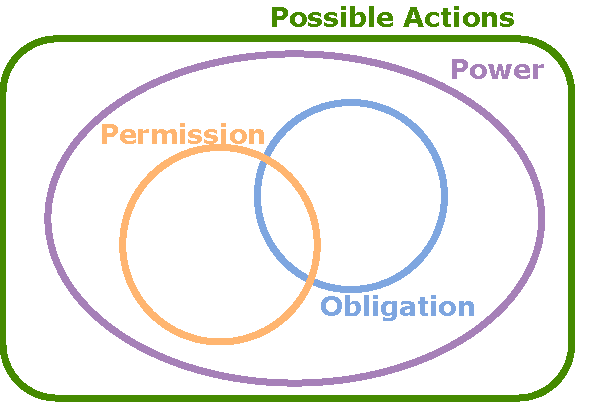
\includegraphics[width=0.6\textwidth]{05_iigo/images/SOMAS_per_obl.pdf}
\caption{Relationship between \emph{power}, \emph{permission} and \emph{obligation}.}
\label{fig:per_obl_sets}
\end{figure} 


For example, the Judge has the \emph{power} to carry out investigations at an IIGO session. There are no rules specifying which specific islands the Judge should investigate. Therefore, the Judge has the \emph{permission} to investigate any `alive' islands during a session. However, the Judge is \emph{obliged} to make at least some number of investigations each turn.



\section{Executive Branch}
\label{sec:executive}
The executive branch is responsible for \textbf{carrying out the law}.
\begin{itemize}
       
    \item The President has the \emph{power} to: 
    \begin{itemize}
        
        \item Select a rule for voting $R^{*}$ to be passed to the Speaker.
        \begin{rule_IIGO}
            The President has the \emph{obligation} to \emph{select} a rule $R^{*}$ if the \emph{rule proposal list} has at least one proposed rule in it.
        \end{rule_IIGO}
        \begin{rule_IIGO}
            The President has the \emph{permission} to \emph{select} a rule $R^{*}$ if and only if $R^{*} \in S$, where $S$ is the \emph{rule proposal list}.
        \end{rule_IIGO}
        
        \item Decide the amount of individual \emph{taxation} (i.e. a specific \emph{minimum} amount of contribution to the common pool for each island) for the current turn.
        
        \begin{itemize}
            \item The President is given the self-reported resource amounts held by each island to assist in this decision.
            %\item Suggested Rule: For any island that has chosen to not report it's resources, the President has the \emph{obligation} to set them an individual tax amount T.
        \end{itemize}
        
        \item Decide the allocation of resources distributed from the common pool to the islands (i.e. a specific \emph{maximum} amount an island is permitted to take from the common pool).
        
        \begin{itemize}
            \item The President is given the \emph{allocation requests} made by each island.
            %\item \emph{}{Suggested Rule:} The President has an obligation to prioritise islands in critical condition.
        \end{itemize}
    \end{itemize}
\end{itemize}



\section{Legislative Branch}
\label{sec:legislative}
The legislative branch is responsible for \textbf{making the law}.
\begin{itemize}

    \item The Speaker has the \emph{power} to:
    \begin{itemize}
        
        \item Call a vote $V$ for a rule $R$.
        \begin{rule_IIGO}
            The Speaker has the \emph{obligation} to \emph{call} a vote $V$ if and only if the President has \emph{selected} a rule $R$ to be voted on.
        \end {rule_IIGO}
        \begin{rule_IIGO}
            The Speaker has the \emph{permission} to \emph{call} a vote $V$ for a rule $R$ if and only if the rule $R = R^{*}$, where $R^{*}$ is the rule \emph{selected} by the President.
        \end {rule_IIGO}
            
        \item Choose which islands are participating in the vote $V$.
       % \footnote{This is our sequential implementation alternative for the power to close the ballot box.}.
        \begin{rule_IIGO}
            The Speaker has the \emph{obligation} to ask for a vote from all alive islands.
        \end {rule_IIGO}
            
        \item Declare the result $C$ of a vote $V$. 
        \begin{rule_IIGO}
            The Speaker has the \emph{obligation} to \emph{declare the result} $C$ for a vote $V$ if and only if the vote V has been \emph{called}.
        \end {rule_IIGO}
        \begin{rule_IIGO}
            The Speaker has the \emph{permission} to \emph{declare the result} $C$ for a vote $V$ if $C = C^{*}$, where $C^{*}$ is the result produced by \emph{calling} the vote $V$.
        \end {rule_IIGO}
        \begin{itemize}
            \item This step is what enables a rule to be \emph{active}.
        \end{itemize}
    \end{itemize}
\end{itemize}




\section{Judicial Branch}
\label{sec:judicial}

The judicial branch is responsible for \textbf{evaluating the law}.
\begin{itemize}
    \item The Judge has the \emph{power} to:
    \begin{itemize}
        \item Perform a number of \emph{inspections}\footnote{An \emph{inspection} \textbf{costs} an expense of resources (See Definition~\ref{def:invst} for more detail).} $I$ and produce a compliance outcome $\mathbb{O}^{*}$\footnote{Note that the compliance outcome $\mathbb{O}^{*}$ considered is a boolean.}.
        %(true: the island has been compliant with the rules in play, false: the island has not been compliant with the rules in play)
        %\begin{itemize}
           % \item For example, to check if the event outcome is \emph{concurrent}\footnote{Again, what is defined as "concurrent"? A clear definition is needed.} with the rules.
        %\end{itemize}
        \begin{rule_IIGO}
            The Judge has the \emph{obligation} to make at least $N$ investigations at each turn.
        \end{rule_IIGO}
        \item Declare the outcome $\mathbb{O}$ of an inspection $I$ to all islands\footnote{This act of broadcasting is especially important for islands to form an opinion about the sanctioned islands accordingly.}.
        \begin{rule_IIGO}
            The Judge has the \emph{obligation} to declare the outcome $\mathbb{O}$ of an inspection $I$ if and only if the inspection $I$ has been performed.
        \end{rule_IIGO}
        \begin{rule_IIGO}
            The Judge has the \emph{permission} to declare the outcome $\mathbb{O}$ of an inspection $I$ if $\mathbb{O} = \mathbb{O}^{*}$, where $\mathbb{O}^{*}$ is the outcome of the inspection $I$.
        \end{rule_IIGO}
        %\item Initiate the removal of the \texttt{President}.
        %\begin{itemize}
            %\item A good Judge would be especially vigilant during \emph{power transfer} regarding the \emph{President} position (see Section~\ref{leg_const} for more detail).
        %\end{itemize}
        \item Invoke economic \textbf{sanctions} (see Section~\ref{sec:sanctions} for more detail).
        \begin{rule_IIGO}
            The Judge has the \emph{obligation} to invoke a sanction $S$ for an island $X$ if and only if an investigation $I$ has an outcome $\mathbb{O}^{*}$ indicating non-compliance, and $I$ is an investigation of an action taken by island $X$.
        \end{rule_IIGO}
        \item Invoke even more severe sanctions in the case of further disobedience to previous sanction(s).
        \begin{rule_IIGO}
            The Judge has the \emph{permission} to invoke a severer sanction $S'$ for an island $X$ if the island $X$ has not fulfilled the requirements of the previous sanction $S$.
        \end{rule_IIGO}
        \item Pardon the islands which are currently sanctioned.
        \begin{rule_IIGO}
            The Judge has the \emph{permission} to revoke any sanction $S$ of an island $X$ at a specific turn.
        \end{rule_IIGO}
    \end{itemize}
\end{itemize}
%(e.g. a new rule that falls under a "sanction" category \hl{[I'm not sure about this being a `new rule` [Ezgi]]}

\subsection{Sanctions}
\label{sec:sanctions}
All sanctions are of economic nature which include:
        \begin{itemize}
            %\item Revoking an island's access to the common pool.
            \item Enforcing an island to contribute a specific amount of resources to the common pool.
            \begin{itemize}
                \item This does not mean that the Judge has the \emph{power} to take resources from an island in order to put them to the common pool -- the island itself is expected to carry out this implication imposed by the sanction itself, otherwise further punishment can be induced by the Judge.
                \item Similarly, \emph{opinion formulation} will follow accordingly whether the island(s) is/are following the implications imposed by the sanction(s).
            \end{itemize}
        
    \end{itemize}
    Sanctions are the associated penalty that comes with an island breaking a specific rule. The Judge is in full control of the penalties associated with breaking any rules. Once the Judge has specified the score of the penalty associated with each time an island breaks a rule, the cumulative penalties accumulated by the island are then used to determine which \textbf{sanction tier} that each island falls into. The score threshold to determine the boundaries of the sanction tiers are set by the Judge. At each turn of the game, each island is told whether they are being sanctioned, and if so, which \textbf{sanction tier} that they are currently in. The \textbf{sanction tiers} of the non-compliant islands are also broadcasted to the other islands in the archipelago. To summarise, the sanctioning process follows these steps:
    
    
    
    %Sanctions are based on an island breaking a rule. Each rule must therefore have an associated penalty. By default, we set these penalties such that they add $1$ to the total sanction score for each island. However, we allow the judge to override this scoring, the judge is able to set their own scores for any particular rule as they desire. This custom scoring is then used when an island breaks a particular rule. By looking at events that occurred in the last turn, and using the customised scoring we provide the holder of the judge role with full control of the penalties for breaking any rules.
    
    





%we then use the cumulative penalties accumulated by each island to determine which Sanction Tier they fall into. The score threshold's required to fall into these sanction tiers is set by the judge and is checked for monotonicity. Each island is told whether they are being sanctioned, and is so what tier they are in. We also tell other islands about which sanction tiers other islands have fallen into. 

    \begin{enumerate}
        \item The Judge has the \emph{power} to set custom penalties associated with breaking any rules.
        \item The Judge is given a list of all events that occurred in the previous turn.
        \item The Judge has the \emph{power} to check whether any, or all of these previous events, involve the islands in the archipelago breaking any rules.
        \item Each of the transgressions is scored using the Judge's custom penalties if the Judge has set them. Otherwise, a score of $1$ is given each time a rule is broken.
        \item The Judge has the \emph{power} to revise the sanction thresholds.
        \item Using the latest sanction thresholds available, each island is assigned to a sanction tier based on the sanction score that it has received.
        \item These sanction tiers are broadcasted to all of the islands in the archipelago.
        \item The Judge then uses sanctions rules in place to calculate the specific amount of resources that each non-compliant island has in order to determine how much it should contribute to the common pool, based on the sanction tier that it is in.
    \end{enumerate}



\section{Constitutional Rights and Obligations in the Archipelago}
\label{sec:const_rights_obl_archi}
Each island has the \emph{power} to:
\begin{itemize}
\item make an \emph{allocation request} (see Definition~\ref{def:alloc_req}) to the President for a specific amount to be allocated to them.
\item report the number of resources it is in possession of to the President.
\begin{rule_IIGO}
    Each island has the \emph{obligation} to report the number of resources it is in possession of to the President.
\end{rule_IIGO}
\begin{rule_IIGO}
    Each island has the \emph{permission} to report the number of resources $R'$ if and only if $R' = R$, where R is the number of resources the island is in possession of.
\end{rule_IIGO}
\item take resources from the common pool.


\begin{rule_IIGO}
    Each island has the \emph{permission} to take at maximum $N$ resources, where $N$ is the specific allocation made by the President to that island\footnote{If no such allocation is made, the island is \emph{permitted} to take any amount of resources.}.
\end{rule_IIGO}
\item contribute resources to the common pool.
\begin{rule_IIGO}
    Each island has the \emph{obligation} to contribute to the common pool an amount greater or equal to that of the individual tax set by the President.
\end{rule_IIGO}
                %The President is in
                %(unless there is a rule in place that dictates how Speaker is to allocate resources).
\item add a rule to the \emph{rule proposal list} (see Definition~\ref{def:rule_prop_list}) at the start of each turn.
        %\begin{itemize}
            %\item The game specification includes how many rules an island can propose each turn.
        %\end{itemize}
        %\item vote  for rules in the Legislative Branch and vote for their favourite islands in elections
\item participate in the legislative branch of the government by casting ballots in votes called by the Speaker
\item vote for an island to be elected for a specific role (e.g. the President, Judge, Speaker) during the elections\footnote{This will be assumed to be true \underline{unless stated otherwise}. %Note that \textbf{diplomatic sanctions} can disable this power of a specific island (see Section~\ref{jud_const}).}.
        }.
\end{itemize}
\section{Accountability Cycle}
\label{sec:accountability}


To ensure that the government avoids corruption and abuse of power, each branch is accountable to another. The President is accountable to the Speaker, the Speaker is accountable to the Judge, and the Judge is accountable to the President (see Figure~ \ref{fig:cycles_in_IIGO}). This accountability cycle is enacted through \emph{monitoring} actions\footnote{Note that the terms \textbf{monitoring} and \textbf{investigation} have similar but quite different meanings in the IIGO context.}. 

The powers related to the accountability cycle and transfer-of-power for each role can be summarized as the following: 
\begin{itemize}
    \item The Speaker has the \emph{power} to: 
    \begin{itemize}
        \item monitor the President.
        \item announce the result of this monitoring.
        \item initiate the transfer-of-power for the Judge.
    \end{itemize}
    \item The President has the \emph{power} to: 
    \begin{itemize}
        \item monitor the Judge.
        \item announce the result of this monitoring.
        \item initiate the transfer-of-power for the Speaker.
    \end{itemize}
    \item The Judge has the \emph{power} to: 
    \begin{itemize}
        \item  monitor the Speaker.
        \item announce the result of this monitoring.
        \item initiate the transfer-of-power for the President.
    \end{itemize}
\end{itemize}

%Unlike investigations performed by the Judge, who performs investigations on island actions in the following turn, each role is given the opportunity to check up on the actions of the role it is responsible for immediately after they have been performed. In this sense, the President can monitor (includes investigative-monitoring) the powers (calling a vote and announcing the result) acted on by the Speaker immediately after the Speaker's announcement (or lack there of). The government officials hold a lot of power so this is to ensure that any wrong-doing is determined as quickly as possible. For this project we are only pursuing one degree of monitoring, that is, the powers relating to the accountability cycle will not be monitored themselves. We assume that agents will act in the interest of themselves and keeping all the islands alive is beneficial to everyone. Hence, while the agents might be inclined to break rules in order to benefit themselves, anyone else breaking the rules is seen as undesirable under the assumption that the system in place is there to benefit all. 


Through the proposed accountability cycle, each role is given the opportunity to check up on the actions of the role it is accountable for immediately after they have been performed. It is clear that the IIGO roles (i.e. the President, Speaker and Judge) hold a considerable amount of \emph{power} in their hands. The accountability cycle is designed to address the possible abuses of this power. With monitoring, any wrong-doing in the IGO is determined as quickly as possible and the role in question can be replaced. 

Within the scope of the coursework, we decided to pursue only \emph{one degree of monitoring}, meaning that the powers relating to the accountability cycle will not be monitored themselves. We assume that agents will act in the interest of all the islands in the archipelago. Hence, while the agents might be inclined to break the rules to benefit in some form, it is assumed that the others will negatively see any non-compliant islands based on the assumption that the proposed IIGO system is in place to maintain the welfare of all the islands.

Let role $X$ be accountable to the role $Y$, which is accountable to the role $Z$. Then:
\begin{rule_IIGO}
$Y$ has the \emph{obligation} to declare the outcome of the monitoring result $M$ associated with the action $A$ undertaken by $X$ if and only if $Y$ has monitored the action $A$ performed by $X$. 
\end{rule_IIGO}
\begin{rule_IIGO}
$Y$ has the \emph{permission} to declare the monitoring result $M$ associated with the action $A$ undertaken by $X$ if and only if $M = M^{*}$, where $M^{*}$ is the outcome of \emph{monitoring} action $A$ performed by $X$\footnote{These constitutional rules should be available to the agents to check their decision against. However, due to having only one degree of accountability cycle in place, these rules are not enforced through any sanctions (i.e. breaking these rules has no consequences as they only deem to be an \emph{agreement} among the roles).}.
\end{rule_IIGO}


\begin{figure}[!htb]
\centering
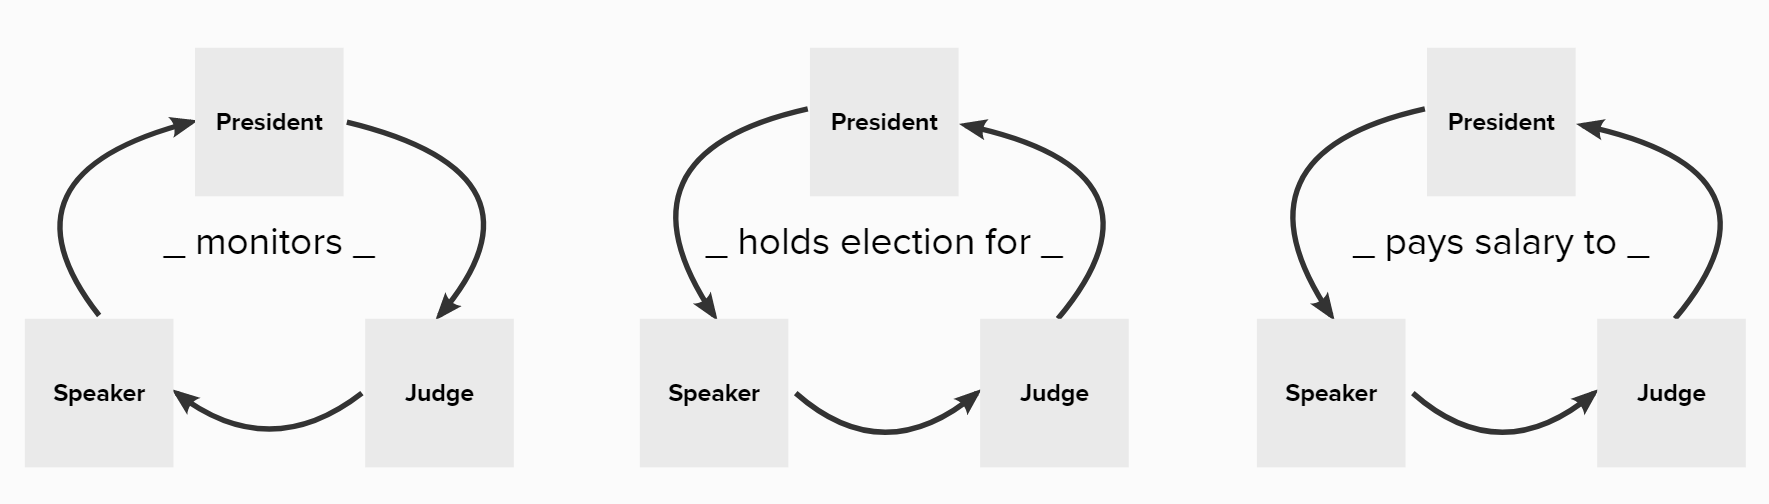
\includegraphics[scale=0.33]{05_iigo/images/role cycles.png}
\caption{Accountability cycle (left), the transfer-of-power cycle (middle) and salary cycle (right).}
\label{fig:cycles_in_IIGO}
\end{figure}


\subsection{Transfer-of-power}
\label{subsec:transfer-of-power}
\begin{enumerate}
    \item The Speaker conducts a vote for the election of the new Judge.
    \item The Judge conducts a vote for the election of the new President.
    \item The President conducts a vote for the election of the new Speaker.
\end{enumerate}
Refer to the Figure~ \ref{fig:cycles_in_IIGO} for further clarification about the transfer-of-power cycle.

\begin{rule_IIGO}
   The role $X$ has the \emph{obligation} to conduct a vote for the election of $Y$ at the end of the term (see Definition~\ref{def:term}) if and only if the role $X$ is accountable to the role $Y$. 
\end{rule_IIGO}.

\section{Budget and Salary}
\subsection{Budget}
%Actions associated with the IIGO have an associated cost that is defined as a configuration parameter. The institutional-power-enabled actions of  identified to require a "computational" component are:

Institutional-enabled-power actions in the IIGO have an associated cost with them. Some examples for such actions include:


%that is defined as a configuration parameter. The institutional-power-enabled actions of  identified to require a "computational" component are:


%We have defined the resource to be an endogenous one, hence any computation surrounding the distribution of the resource must use up some of that resource. 
\begin{itemize}
\item Calling any vote and computing the winner.
\item Declaring (e.g. \textit{announcing} the result of a vote).
\item Setting the amount of \emph{taxation} for each island.
\item Deciding the allocation distribution for each island.
\item Inspecting an island's action history.
\item Monitoring a role.
\end{itemize}

Since IIGO has been designed to act in the common good, IIGO-related costs will be directly withdrawn from the common pool. Since the common pool is considered a communal property of the archipelago, there are rules in place to limit how much each role is allowed to spend in order to perform its own institutional-power-enabled actions. This is the reason why defining the \emph{budget} and keeping it separate for each of the three IIGO roles.


As a role performs institutional-enabled-power actions, the corresponding cost associated with this action is subtracted from the role's budget. A budget of zero means that the role does not have the \emph{power} to perform any of its institutional-power-enabled actions. The removal of the budget rule from the rules in play means the role is allowed to perform as many such actions as it prefers to (as long as those actions are not governed by other rules). 



%As a role performs an endogenous-cost action, the corresponding cost associated with this action is subtracted from the role's budget. Thus, if as a result of an endogenous-cost action a role will be left with negative budget, it will have gone over the budget limit and will have broken the budget rule. A budget of zero means that the role is not allowed to perform any of its institutional-power-enabled actions associated an endogenous-cost. The removal of the budget rule from the rules in play means the role is allowed to perform as many such actions as it pleases (as long as those actions are not governed by other rules). 

The budget rule is also persistent across turns. This means that, assuming nothing else affects the budget, if a role has $100$ resources in its budget at each turn and spends only $10$ resources, this means that this very same role has $90$ resources in its budget at the next turn. On the other hand, islands can choose to increase the budget periodically every turn. This is governed by another budget extension rule.




%one turn and it spends 10, it has 90 resources in it's budget the next turn. 

Finally, it must be noted that the budget is inherently linked with the fact that whether obligations of a specific role can be undergone.
For example, during \emph{monitoring}, it should not be seen as a rule violation if a role has not acted on an obligation if it would go over the budget as a result. 

%This can also be seen as an added clause "... and the action is only permitted if they have the budget" to most rules which govern actions with an endogenous-cost.
%\begin{rule_IIGO}
    %The budget is increased by an amount $N$ every turn.
%\end{rule_IIGO}

%This rule means that, assuming nothing else affects the budget, if a budget is set to increase by 10 resources every turn and the budget is a 100 resources in turn one, the budget is 110 resources in turn 2. Setting this rule to 0 is equal to removing this rule and it means that the budget is never increased. 


\subsection{Salary}
\label{subsec:salary}
A salary is paid to each role in power as an incentive to act in a publicly approved way. %Hence, each role has the \emph{power} to pay a salary to another role following the salary cycle in Figure~\ref{fig:cycles_in_IIGO}.
\begin{rule_IIGO} \label{rule:salary}
   %Each role has the \emph{obligation} to pay the salary of amount $S$ to another if and only if the amount paid $S'$ is equal to $S$.
   Each role has the \emph{obligation} to pay the salary of amount $S$ to one another following the salary cycle in Figure~\ref{fig:cycles_in_IIGO}.
\end{rule_IIGO}

In Rule~\ref{rule:salary}, setting $S=0$ (through changing the active rules in place) means that roles do not have the permission to pay any salary. Removing the Rule~\ref{rule:salary} means that the roles may freely choose the amount $S$ for the salary payments.

\section{IIGO Session order}

\begin{enumerate}
    \item The Judge has the \emph{power} to check the history of actions to confirm whether the previously punished island(s) has/have obeyed the previous round's sanctions, meaning whether they contributed to the common pool accordingly in case of economic sanctions.
    %\begin{itemize}
      %  \item \emph{Suggested Rule:} In case of disobeying sanctions, the Judge is \emph{obliged} and \emph{permitted} to increase the severity of sanctions with respect to specific islands.
   % \end{itemize}
    \item The Judge has the \emph{power} to carry out \emph{inspections} on the history of actions of any island $X$ to check whether:
        \begin{enumerate}
        \item the reported resources of $X$ in the previous round match the real value of resources $X$ had in its private pool for the previous turn.
        \item the island $X$ has retrieved the right amount of the resources from the common pool, based on the \emph{allocation request} evaluated by the previous President.
            \begin{itemize}
            \item An example: In the previous round, the President has decided that the island $X$ can take $Y$ amount of resources from the common pool. If the Judge finds out that the island $X$ has taken an amount of $Y'$ such that $Y' > Y$, the Judge has the \emph{power} to invoke sanctions on the island $X$.
            
            %the Judge is \emph{obliged} and \emph{permitted} to sanction island $X$.
            \end{itemize}
        \end{enumerate}
    \item The Judge has the \emph{power} to invoke sanctions based on the outcome of the inspections.
    \item The President has the \emph{power} to decide to carry out a \emph{monitoring} on:
        \begin{enumerate}
        \item the sanctions imposed by the Judge.
        \end{enumerate}
    \item The islands may report the resources in their private pools to the President.
    \item The President has the \emph{power} to let each island know about the amount of \emph{taxation} they have to pay.
    \item The island has the \emph{power} to make an \emph{allocation request} to the President.
    \item The President has the \emph{power} decide on an allocation of resources and let each island know about the amount of resource allocation they are permitted to take from the common pool.
    \item The island has the \emph{power} to pick and to propose a rule to be voted on to the President.
    \item The President has the \emph{power} to choose a rule to be voted on from the received rule proposals.
    \item The Speaker has the \emph{power} to decide to carry out a \emph{monitoring} on: 
        \begin{enumerate}
        \item the resource allocation decided by the President.
        \item the rule proposed by the President.
        \end{enumerate}
    \item The Speaker has the \emph{power} to call a vote.
        \begin{enumerate}
        \item The islands vote in support of, or against, the rule (aye or nay) anonymously.
        \end{enumerate}
    \item The Speaker has the \emph{power} to announce a result of a vote to the islands and carries out the law change, if required (e.g. deleting/rejecting a rule if there is a majority nay vote).
    \item The Judge has the \emph{power} to decide to carry out \emph{monitoring} on:
        \begin{enumerate}
        \item the vote called by the Speaker.
        \item the Speaker announcing the result.
    \end{enumerate}
    \item The roles pay salary for one another following the accountability cycle in Figure~ \ref{fig:cycles_in_IIGO}.

\end{enumerate}



\section{Future Work}

\begin{itemize}
    \item \textbf{Diplomatic sanctions}: Although having the potential of being a good alternative for severer sanctions discussed in  Section~\ref{sec:sanctions}, diplomatic sanctions are \emph{not} implemented within the scope of the coursework. \\
    Suggested diplomatic sanctions include:
        \begin{itemize}
            \item Revoking an island's eligibility to vote and to be elected for a position.
            \item Revoking an island's eligibility to propose a rule/motion.
        \end{itemize}
    \item \textbf{Immutable rules}: Within the scope of the coursework, a subset of rules could have been categorised as immutable. This means that to change such immutable rules, the islands first need to vote to change their status to be \emph{mutable}, and consequently, hold another vote to change these mutable rules.
    %\item \textbf{Adding rules to the proposal list: } 
\end{itemize}

    \chapter{Inter-Island Governmental Organisation (IIGO)}


The role of IIGO is to maintain, update, and revise the rules concerning provision to managing the long-term collective risk dilemma (ltCRD). 

\begin{itemize}
    \item There will be 3 distinct branches in the IIGO: the \textbf{legislative branch}, \textbf{executive branch} and \textbf{judicial branch}\footnote{This is, as no surprise, inspired by the separation of powers in Western democracies.}.
    \item Each role is put in power according to the  transfer-of-power rules (see Section~\ref{subsec:transfer-of-power} for more detail).
    \item The head of the legislative branch is the Speaker, the head of the executive branch is the President, and the head of judicial branch is the Judge.
    \begin{itemize}
        \item  The Speaker, President and Judge are selected, through a democratic election, from the islands in the archipelago\footnote{This naming is inspired by the roles in the US Government.}.
        \item The resources gathered by the archipelago are endogenous, hence acting on the institutional powers granted to the Speaker, President or Judge costs resources. 
        \item For their duty, the President, the Speaker and the Judge receive a salary for each of their turns in office (see Section~\ref{subsec:salary} for more detail).
        \item The limit of the powers of the President, Speaker and Judge are defined in this chapter (e.g. the Speaker can only call one vote per turn).
 
    \end{itemize}
\end{itemize}

\subsection{IIGO Specific Definitions}
\begin{definition} \label{def:ballot}
    A \textbf{ballot} is related to each island's \textbf{power} to support or disagree with the rule specified in the vote called by the President and to vote in favour or against an island for a specific role (i.e. the President, Speaker, Judge) at each round of the game.
\end{definition}


%\begin{definition} \label{def:vote}
    %A \textbf{vote} is related to a role's (i.e. the President, Speaker, Judge) \textbf{power} to call a vote for a specific rule or an election.
%\end{definition}


\begin{definition} \label{def:tax}
    The \textbf{taxation} is related to the President's \textbf{power} to request a specific \underline{\textbf{minimum}} amount of contribution from each island to the common pool at each round of the game. 
\end{definition}

\begin{definition} \label{def:alloc_req}
    An \textbf{allocation request} is related to each island's \textbf{power} to request a specific amount of resource allocation from the President at each round of the game.
\end{definition}


\begin{definition} \label{def:rule_prop_list}
A \textbf{rule proposal list} is related to each island's \textbf{power} to propose a specific rule to be passed to the President at each round of the game.
\end{definition}

\begin{definition} \label{def:invst}
    An \textbf{investigation} is related to the Judge's \textbf{power} to acquire information to make a decision, followed by a calculation of the expected results and checking whether some specific rules have been obeyed, exclusively for the actions carried out by the \textbf{islands}. 
\end{definition}


An example of an \emph{investigation}: The President has permitted the island $X$ to take the amount of $Y$ resources from the common pool. Upon \emph{investigation} carried out by the Judge, it is revealed that the amount of resources taken out from the common pool by the island $X$ is, in fact, $Y'$ such that $Y' \neq Y$.


\begin{definition}
\textbf{Monitoring} is a government official's \textbf{power} to perform event recognition and to check whether some specific rules have been obeyed.
\end{definition}

An example of \emph{monitoring}: The Speaker has performed only the following action: \emph{counted the votes and calculated the result} for a rule. Upon \emph{monitoring} carried out by the President, it is noticed that the Speaker has not made any \emph{announcement}. Hence, the Speaker has not followed their obligation to \emph{announce} the result of any vote held.

See Section~\ref{sec:accountability} for more information about which roles can monitor which ones.


\begin{definition}
\textbf{Investigative-monitoring} is a government official's \textbf{power} to acquire the information used in acting on a governmental power followed by calculation of the expected results and checking whether some specific rules have been obeyed, exclusively for the actions carried out by a government official they are responsible for.
\end{definition}

An example of \emph{investigative-monitoring}: The Speaker has performed the following actions: \emph{counted the votes and calculated the result $R$} for a vote $V$ and \emph{announced} the result $R'$ for the vote $V$. Upon \emph{investigative-monitoring} carried out by the President, it is noticed that $R' \neq R$. Hence, the Speaker has modified the announced result.


\begin{definition}
The \textbf{sanction} is related to the Judge's \emph{power} to punish non-compliant islands when their disobedience is confirmed through investigations at a specific turn.
\end{definition}


\begin{definition}
The (judicial) \textbf{pardon} is related to the Judge's \emph{power} to forgive a non-compliant island at a specific turn.
\end{definition}

\begin{definition}
The \textbf{budget} is the maximum amount of resources a role is permitted to spend from the common pool as it performs its own institutional-power-enabled actions at a specific turn.
\end{definition}


\begin{definition}
The \textbf{salary} is the amount of resources a role is to be given from the common pool as a reward for performing its institutional-power-enabled actions at a specific turn.
\end{definition}

\begin{definition} \label{def:term}
A \textbf{term} is the number of turns an island is \emph{permitted} to hold a role, and after which the responsible role (indicated in the transfer-of-power cycle in Figure~\ref{fig:cycles_in_IIGO}) is \emph{obliged} to initiate transfer-of-power.
\end{definition}

\subsection{\emph{Power}, \emph{Permission} and \emph{Obligation} Distinction}
In the rest of the specifications, we will be specifically using the following three terms to define the actions and responsibilities carried out by the Speaker, President, Judge (see Figure~ \ref{fig:per_obl_sets}):
\begin{itemize}
    \item Power
    \item Permission
    \item Obligation
\end{itemize}



\begin{figure}[H] 
\centering
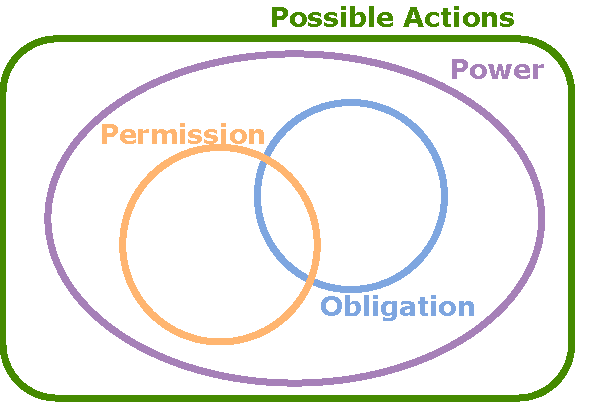
\includegraphics[width=0.6\textwidth]{05_iigo/images/SOMAS_per_obl.pdf}
\caption{Relationship between \emph{power}, \emph{permission} and \emph{obligation}.}
\label{fig:per_obl_sets}
\end{figure} 


For example, the Judge has the \emph{power} to carry out investigations at an IIGO session. There are no rules specifying which specific islands the Judge should investigate. Therefore, the Judge has the \emph{permission} to investigate any `alive' islands during a session. However, the Judge is \emph{obliged} to make at least some number of investigations each turn.



\section{Executive Branch}
\label{sec:executive}
The executive branch is responsible for \textbf{carrying out the law}.
\begin{itemize}
       
    \item The President has the \emph{power} to: 
    \begin{itemize}
        
        \item Select a rule for voting $R^{*}$ to be passed to the Speaker.
        \begin{rule_IIGO}
            The President has the \emph{obligation} to \emph{select} a rule $R^{*}$ if the \emph{rule proposal list} has at least one proposed rule in it.
        \end{rule_IIGO}
        \begin{rule_IIGO}
            The President has the \emph{permission} to \emph{select} a rule $R^{*}$ if and only if $R^{*} \in S$, where $S$ is the \emph{rule proposal list}.
        \end{rule_IIGO}
        
        \item Decide the amount of individual \emph{taxation} (i.e. a specific \emph{minimum} amount of contribution to the common pool for each island) for the current turn.
        
        \begin{itemize}
            \item The President is given the self-reported resource amounts held by each island to assist in this decision.
            %\item Suggested Rule: For any island that has chosen to not report it's resources, the President has the \emph{obligation} to set them an individual tax amount T.
        \end{itemize}
        
        \item Decide the allocation of resources distributed from the common pool to the islands (i.e. a specific \emph{maximum} amount an island is permitted to take from the common pool).
        
        \begin{itemize}
            \item The President is given the \emph{allocation requests} made by each island.
            %\item \emph{}{Suggested Rule:} The President has an obligation to prioritise islands in critical condition.
        \end{itemize}
    \end{itemize}
\end{itemize}



\section{Legislative Branch}
\label{sec:legislative}
The legislative branch is responsible for \textbf{making the law}.
\begin{itemize}

    \item The Speaker has the \emph{power} to:
    \begin{itemize}
        
        \item Call a vote $V$ for a rule $R$.
        \begin{rule_IIGO}
            The Speaker has the \emph{obligation} to \emph{call} a vote $V$ if and only if the President has \emph{selected} a rule $R$ to be voted on.
        \end {rule_IIGO}
        \begin{rule_IIGO}
            The Speaker has the \emph{permission} to \emph{call} a vote $V$ for a rule $R$ if and only if the rule $R = R^{*}$, where $R^{*}$ is the rule \emph{selected} by the President.
        \end {rule_IIGO}
            
        \item Choose which islands are participating in the vote $V$.
       % \footnote{This is our sequential implementation alternative for the power to close the ballot box.}.
        \begin{rule_IIGO}
            The Speaker has the \emph{obligation} to ask for a vote from all alive islands.
        \end {rule_IIGO}
            
        \item Declare the result $C$ of a vote $V$. 
        \begin{rule_IIGO}
            The Speaker has the \emph{obligation} to \emph{declare the result} $C$ for a vote $V$ if and only if the vote V has been \emph{called}.
        \end {rule_IIGO}
        \begin{rule_IIGO}
            The Speaker has the \emph{permission} to \emph{declare the result} $C$ for a vote $V$ if $C = C^{*}$, where $C^{*}$ is the result produced by \emph{calling} the vote $V$.
        \end {rule_IIGO}
        \begin{itemize}
            \item This step is what enables a rule to be \emph{active}.
        \end{itemize}
    \end{itemize}
\end{itemize}




\section{Judicial Branch}
\label{sec:judicial}

The judicial branch is responsible for \textbf{evaluating the law}.
\begin{itemize}
    \item The Judge has the \emph{power} to:
    \begin{itemize}
        \item Perform a number of \emph{inspections}\footnote{An \emph{inspection} \textbf{costs} an expense of resources (See Definition~\ref{def:invst} for more detail).} $I$ and produce a compliance outcome $\mathbb{O}^{*}$\footnote{Note that the compliance outcome $\mathbb{O}^{*}$ considered is a boolean.}.
        %(true: the island has been compliant with the rules in play, false: the island has not been compliant with the rules in play)
        %\begin{itemize}
           % \item For example, to check if the event outcome is \emph{concurrent}\footnote{Again, what is defined as "concurrent"? A clear definition is needed.} with the rules.
        %\end{itemize}
        \begin{rule_IIGO}
            The Judge has the \emph{obligation} to make at least $N$ investigations at each turn.
        \end{rule_IIGO}
        \item Declare the outcome $\mathbb{O}$ of an inspection $I$ to all islands\footnote{This act of broadcasting is especially important for islands to form an opinion about the sanctioned islands accordingly.}.
        \begin{rule_IIGO}
            The Judge has the \emph{obligation} to declare the outcome $\mathbb{O}$ of an inspection $I$ if and only if the inspection $I$ has been performed.
        \end{rule_IIGO}
        \begin{rule_IIGO}
            The Judge has the \emph{permission} to declare the outcome $\mathbb{O}$ of an inspection $I$ if $\mathbb{O} = \mathbb{O}^{*}$, where $\mathbb{O}^{*}$ is the outcome of the inspection $I$.
        \end{rule_IIGO}
        %\item Initiate the removal of the \texttt{President}.
        %\begin{itemize}
            %\item A good Judge would be especially vigilant during \emph{power transfer} regarding the \emph{President} position (see Section~\ref{leg_const} for more detail).
        %\end{itemize}
        \item Invoke economic \textbf{sanctions} (see Section~\ref{sec:sanctions} for more detail).
        \begin{rule_IIGO}
            The Judge has the \emph{obligation} to invoke a sanction $S$ for an island $X$ if and only if an investigation $I$ has an outcome $\mathbb{O}^{*}$ indicating non-compliance, and $I$ is an investigation of an action taken by island $X$.
        \end{rule_IIGO}
        \item Invoke even more severe sanctions in the case of further disobedience to previous sanction(s).
        \begin{rule_IIGO}
            The Judge has the \emph{permission} to invoke a severer sanction $S'$ for an island $X$ if the island $X$ has not fulfilled the requirements of the previous sanction $S$.
        \end{rule_IIGO}
        \item Pardon the islands which are currently sanctioned.
        \begin{rule_IIGO}
            The Judge has the \emph{permission} to revoke any sanction $S$ of an island $X$ at a specific turn.
        \end{rule_IIGO}
    \end{itemize}
\end{itemize}
%(e.g. a new rule that falls under a "sanction" category \hl{[I'm not sure about this being a `new rule` [Ezgi]]}

\subsection{Sanctions}
\label{sec:sanctions}
All sanctions are of economic nature which include:
        \begin{itemize}
            %\item Revoking an island's access to the common pool.
            \item Enforcing an island to contribute a specific amount of resources to the common pool.
            \begin{itemize}
                \item This does not mean that the Judge has the \emph{power} to take resources from an island in order to put them to the common pool -- the island itself is expected to carry out this implication imposed by the sanction itself, otherwise further punishment can be induced by the Judge.
                \item Similarly, \emph{opinion formulation} will follow accordingly whether the island(s) is/are following the implications imposed by the sanction(s).
            \end{itemize}
        
    \end{itemize}
    Sanctions are the associated penalty that comes with an island breaking a specific rule. The Judge is in full control of the penalties associated with breaking any rules. Once the Judge has specified the score of the penalty associated with each time an island breaks a rule, the cumulative penalties accumulated by the island are then used to determine which \textbf{sanction tier} that each island falls into. The score threshold to determine the boundaries of the sanction tiers are set by the Judge. At each turn of the game, each island is told whether they are being sanctioned, and if so, which \textbf{sanction tier} that they are currently in. The \textbf{sanction tiers} of the non-compliant islands are also broadcasted to the other islands in the archipelago. To summarise, the sanctioning process follows these steps:
    
    
    
    %Sanctions are based on an island breaking a rule. Each rule must therefore have an associated penalty. By default, we set these penalties such that they add $1$ to the total sanction score for each island. However, we allow the judge to override this scoring, the judge is able to set their own scores for any particular rule as they desire. This custom scoring is then used when an island breaks a particular rule. By looking at events that occurred in the last turn, and using the customised scoring we provide the holder of the judge role with full control of the penalties for breaking any rules.
    
    





%we then use the cumulative penalties accumulated by each island to determine which Sanction Tier they fall into. The score threshold's required to fall into these sanction tiers is set by the judge and is checked for monotonicity. Each island is told whether they are being sanctioned, and is so what tier they are in. We also tell other islands about which sanction tiers other islands have fallen into. 

    \begin{enumerate}
        \item The Judge has the \emph{power} to set custom penalties associated with breaking any rules.
        \item The Judge is given a list of all events that occurred in the previous turn.
        \item The Judge has the \emph{power} to check whether any, or all of these previous events, involve the islands in the archipelago breaking any rules.
        \item Each of the transgressions is scored using the Judge's custom penalties if the Judge has set them. Otherwise, a score of $1$ is given each time a rule is broken.
        \item The Judge has the \emph{power} to revise the sanction thresholds.
        \item Using the latest sanction thresholds available, each island is assigned to a sanction tier based on the sanction score that it has received.
        \item These sanction tiers are broadcasted to all of the islands in the archipelago.
        \item The Judge then uses sanctions rules in place to calculate the specific amount of resources that each non-compliant island has in order to determine how much it should contribute to the common pool, based on the sanction tier that it is in.
    \end{enumerate}



\section{Constitutional Rights and Obligations in the Archipelago}
\label{sec:const_rights_obl_archi}
Each island has the \emph{power} to:
\begin{itemize}
\item make an \emph{allocation request} (see Definition~\ref{def:alloc_req}) to the President for a specific amount to be allocated to them.
\item report the number of resources it is in possession of to the President.
\begin{rule_IIGO}
    Each island has the \emph{obligation} to report the number of resources it is in possession of to the President.
\end{rule_IIGO}
\begin{rule_IIGO}
    Each island has the \emph{permission} to report the number of resources $R'$ if and only if $R' = R$, where R is the number of resources the island is in possession of.
\end{rule_IIGO}
\item take resources from the common pool.


\begin{rule_IIGO}
    Each island has the \emph{permission} to take at maximum $N$ resources, where $N$ is the specific allocation made by the President to that island\footnote{If no such allocation is made, the island is \emph{permitted} to take any amount of resources.}.
\end{rule_IIGO}
\item contribute resources to the common pool.
\begin{rule_IIGO}
    Each island has the \emph{obligation} to contribute to the common pool an amount greater or equal to that of the individual tax set by the President.
\end{rule_IIGO}
                %The President is in
                %(unless there is a rule in place that dictates how Speaker is to allocate resources).
\item add a rule to the \emph{rule proposal list} (see Definition~\ref{def:rule_prop_list}) at the start of each turn.
        %\begin{itemize}
            %\item The game specification includes how many rules an island can propose each turn.
        %\end{itemize}
        %\item vote  for rules in the Legislative Branch and vote for their favourite islands in elections
\item participate in the legislative branch of the government by casting ballots in votes called by the Speaker
\item vote for an island to be elected for a specific role (e.g. the President, Judge, Speaker) during the elections\footnote{This will be assumed to be true \underline{unless stated otherwise}. %Note that \textbf{diplomatic sanctions} can disable this power of a specific island (see Section~\ref{jud_const}).}.
        }.
\end{itemize}
\section{Accountability Cycle}
\label{sec:accountability}


To ensure that the government avoids corruption and abuse of power, each branch is accountable to another. The President is accountable to the Speaker, the Speaker is accountable to the Judge, and the Judge is accountable to the President (see Figure~ \ref{fig:cycles_in_IIGO}). This accountability cycle is enacted through \emph{monitoring} actions\footnote{Note that the terms \textbf{monitoring} and \textbf{investigation} have similar but quite different meanings in the IIGO context.}. 

The powers related to the accountability cycle and transfer-of-power for each role can be summarized as the following: 
\begin{itemize}
    \item The Speaker has the \emph{power} to: 
    \begin{itemize}
        \item monitor the President.
        \item announce the result of this monitoring.
        \item initiate the transfer-of-power for the Judge.
    \end{itemize}
    \item The President has the \emph{power} to: 
    \begin{itemize}
        \item monitor the Judge.
        \item announce the result of this monitoring.
        \item initiate the transfer-of-power for the Speaker.
    \end{itemize}
    \item The Judge has the \emph{power} to: 
    \begin{itemize}
        \item  monitor the Speaker.
        \item announce the result of this monitoring.
        \item initiate the transfer-of-power for the President.
    \end{itemize}
\end{itemize}

%Unlike investigations performed by the Judge, who performs investigations on island actions in the following turn, each role is given the opportunity to check up on the actions of the role it is responsible for immediately after they have been performed. In this sense, the President can monitor (includes investigative-monitoring) the powers (calling a vote and announcing the result) acted on by the Speaker immediately after the Speaker's announcement (or lack there of). The government officials hold a lot of power so this is to ensure that any wrong-doing is determined as quickly as possible. For this project we are only pursuing one degree of monitoring, that is, the powers relating to the accountability cycle will not be monitored themselves. We assume that agents will act in the interest of themselves and keeping all the islands alive is beneficial to everyone. Hence, while the agents might be inclined to break rules in order to benefit themselves, anyone else breaking the rules is seen as undesirable under the assumption that the system in place is there to benefit all. 


Through the proposed accountability cycle, each role is given the opportunity to check up on the actions of the role it is accountable for immediately after they have been performed. It is clear that the IIGO roles (i.e. the President, Speaker and Judge) hold a considerable amount of \emph{power} in their hands. The accountability cycle is designed to address the possible abuses of this power. With monitoring, any wrong-doing in the IGO is determined as quickly as possible and the role in question can be replaced. 

Within the scope of the coursework, we decided to pursue only \emph{one degree of monitoring}, meaning that the powers relating to the accountability cycle will not be monitored themselves. We assume that agents will act in the interest of all the islands in the archipelago. Hence, while the agents might be inclined to break the rules to benefit in some form, it is assumed that the others will negatively see any non-compliant islands based on the assumption that the proposed IIGO system is in place to maintain the welfare of all the islands.

Let role $X$ be accountable to the role $Y$, which is accountable to the role $Z$. Then:
\begin{rule_IIGO}
$Y$ has the \emph{obligation} to declare the outcome of the monitoring result $M$ associated with the action $A$ undertaken by $X$ if and only if $Y$ has monitored the action $A$ performed by $X$. 
\end{rule_IIGO}
\begin{rule_IIGO}
$Y$ has the \emph{permission} to declare the monitoring result $M$ associated with the action $A$ undertaken by $X$ if and only if $M = M^{*}$, where $M^{*}$ is the outcome of \emph{monitoring} action $A$ performed by $X$\footnote{These constitutional rules should be available to the agents to check their decision against. However, due to having only one degree of accountability cycle in place, these rules are not enforced through any sanctions (i.e. breaking these rules has no consequences as they only deem to be an \emph{agreement} among the roles).}.
\end{rule_IIGO}


\begin{figure}[!htb]
\centering
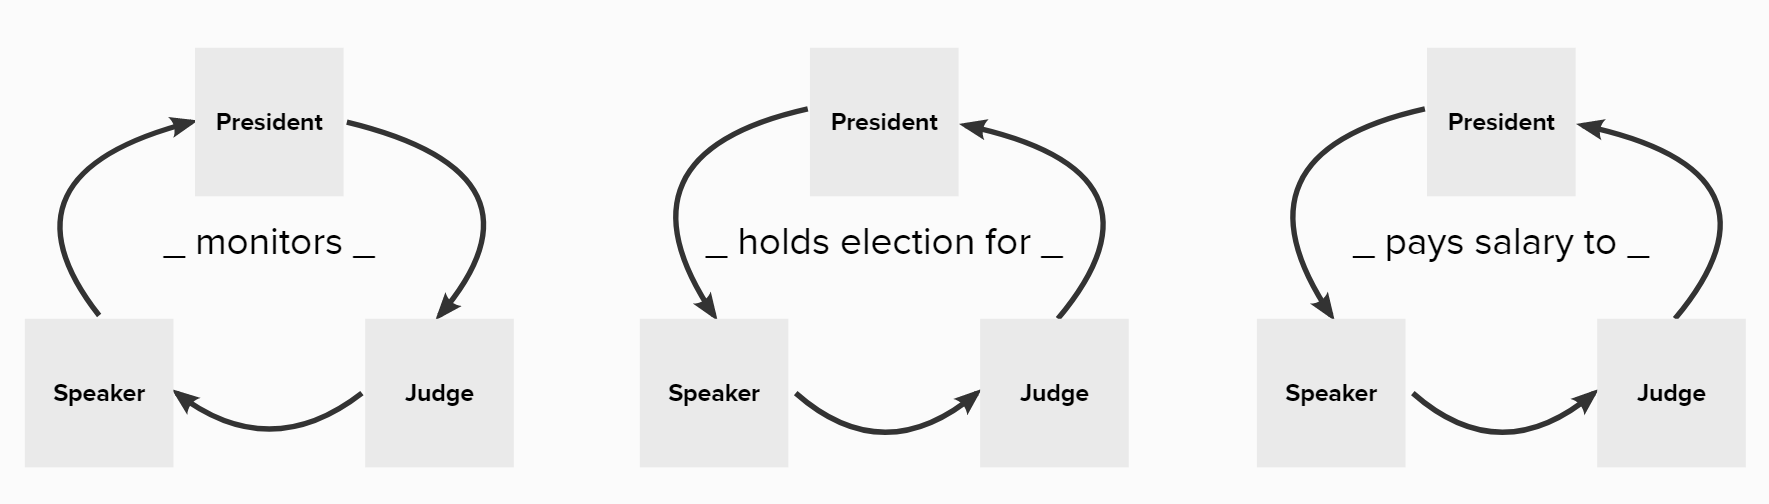
\includegraphics[scale=0.33]{05_iigo/images/role cycles.png}
\caption{Accountability cycle (left), the transfer-of-power cycle (middle) and salary cycle (right).}
\label{fig:cycles_in_IIGO}
\end{figure}


\subsection{Transfer-of-power}
\label{subsec:transfer-of-power}
\begin{enumerate}
    \item The Speaker conducts a vote for the election of the new Judge.
    \item The Judge conducts a vote for the election of the new President.
    \item The President conducts a vote for the election of the new Speaker.
\end{enumerate}
Refer to the Figure~ \ref{fig:cycles_in_IIGO} for further clarification about the transfer-of-power cycle.

\begin{rule_IIGO}
   The role $X$ has the \emph{obligation} to conduct a vote for the election of $Y$ at the end of the term (see Definition~\ref{def:term}) if and only if the role $X$ is accountable to the role $Y$. 
\end{rule_IIGO}.

\section{Budget and Salary}
\subsection{Budget}
%Actions associated with the IIGO have an associated cost that is defined as a configuration parameter. The institutional-power-enabled actions of  identified to require a "computational" component are:

Institutional-enabled-power actions in the IIGO have an associated cost with them. Some examples for such actions include:


%that is defined as a configuration parameter. The institutional-power-enabled actions of  identified to require a "computational" component are:


%We have defined the resource to be an endogenous one, hence any computation surrounding the distribution of the resource must use up some of that resource. 
\begin{itemize}
\item Calling any vote and computing the winner.
\item Declaring (e.g. \textit{announcing} the result of a vote).
\item Setting the amount of \emph{taxation} for each island.
\item Deciding the allocation distribution for each island.
\item Inspecting an island's action history.
\item Monitoring a role.
\end{itemize}

Since IIGO has been designed to act in the common good, IIGO-related costs will be directly withdrawn from the common pool. Since the common pool is considered a communal property of the archipelago, there are rules in place to limit how much each role is allowed to spend in order to perform its own institutional-power-enabled actions. This is the reason why defining the \emph{budget} and keeping it separate for each of the three IIGO roles.


As a role performs institutional-enabled-power actions, the corresponding cost associated with this action is subtracted from the role's budget. A budget of zero means that the role does not have the \emph{power} to perform any of its institutional-power-enabled actions. The removal of the budget rule from the rules in play means the role is allowed to perform as many such actions as it prefers to (as long as those actions are not governed by other rules). 



%As a role performs an endogenous-cost action, the corresponding cost associated with this action is subtracted from the role's budget. Thus, if as a result of an endogenous-cost action a role will be left with negative budget, it will have gone over the budget limit and will have broken the budget rule. A budget of zero means that the role is not allowed to perform any of its institutional-power-enabled actions associated an endogenous-cost. The removal of the budget rule from the rules in play means the role is allowed to perform as many such actions as it pleases (as long as those actions are not governed by other rules). 

The budget rule is also persistent across turns. This means that, assuming nothing else affects the budget, if a role has $100$ resources in its budget at each turn and spends only $10$ resources, this means that this very same role has $90$ resources in its budget at the next turn. On the other hand, islands can choose to increase the budget periodically every turn. This is governed by another budget extension rule.




%one turn and it spends 10, it has 90 resources in it's budget the next turn. 

Finally, it must be noted that the budget is inherently linked with the fact that whether obligations of a specific role can be undergone.
For example, during \emph{monitoring}, it should not be seen as a rule violation if a role has not acted on an obligation if it would go over the budget as a result. 

%This can also be seen as an added clause "... and the action is only permitted if they have the budget" to most rules which govern actions with an endogenous-cost.
%\begin{rule_IIGO}
    %The budget is increased by an amount $N$ every turn.
%\end{rule_IIGO}

%This rule means that, assuming nothing else affects the budget, if a budget is set to increase by 10 resources every turn and the budget is a 100 resources in turn one, the budget is 110 resources in turn 2. Setting this rule to 0 is equal to removing this rule and it means that the budget is never increased. 


\subsection{Salary}
\label{subsec:salary}
A salary is paid to each role in power as an incentive to act in a publicly approved way. %Hence, each role has the \emph{power} to pay a salary to another role following the salary cycle in Figure~\ref{fig:cycles_in_IIGO}.
\begin{rule_IIGO} \label{rule:salary}
   %Each role has the \emph{obligation} to pay the salary of amount $S$ to another if and only if the amount paid $S'$ is equal to $S$.
   Each role has the \emph{obligation} to pay the salary of amount $S$ to one another following the salary cycle in Figure~\ref{fig:cycles_in_IIGO}.
\end{rule_IIGO}

In Rule~\ref{rule:salary}, setting $S=0$ (through changing the active rules in place) means that roles do not have the permission to pay any salary. Removing the Rule~\ref{rule:salary} means that the roles may freely choose the amount $S$ for the salary payments.

\section{IIGO Session order}

\begin{enumerate}
    \item The Judge has the \emph{power} to check the history of actions to confirm whether the previously punished island(s) has/have obeyed the previous round's sanctions, meaning whether they contributed to the common pool accordingly in case of economic sanctions.
    %\begin{itemize}
      %  \item \emph{Suggested Rule:} In case of disobeying sanctions, the Judge is \emph{obliged} and \emph{permitted} to increase the severity of sanctions with respect to specific islands.
   % \end{itemize}
    \item The Judge has the \emph{power} to carry out \emph{inspections} on the history of actions of any island $X$ to check whether:
        \begin{enumerate}
        \item the reported resources of $X$ in the previous round match the real value of resources $X$ had in its private pool for the previous turn.
        \item the island $X$ has retrieved the right amount of the resources from the common pool, based on the \emph{allocation request} evaluated by the previous President.
            \begin{itemize}
            \item An example: In the previous round, the President has decided that the island $X$ can take $Y$ amount of resources from the common pool. If the Judge finds out that the island $X$ has taken an amount of $Y'$ such that $Y' > Y$, the Judge has the \emph{power} to invoke sanctions on the island $X$.
            
            %the Judge is \emph{obliged} and \emph{permitted} to sanction island $X$.
            \end{itemize}
        \end{enumerate}
    \item The Judge has the \emph{power} to invoke sanctions based on the outcome of the inspections.
    \item The President has the \emph{power} to decide to carry out a \emph{monitoring} on:
        \begin{enumerate}
        \item the sanctions imposed by the Judge.
        \end{enumerate}
    \item The islands may report the resources in their private pools to the President.
    \item The President has the \emph{power} to let each island know about the amount of \emph{taxation} they have to pay.
    \item The island has the \emph{power} to make an \emph{allocation request} to the President.
    \item The President has the \emph{power} decide on an allocation of resources and let each island know about the amount of resource allocation they are permitted to take from the common pool.
    \item The island has the \emph{power} to pick and to propose a rule to be voted on to the President.
    \item The President has the \emph{power} to choose a rule to be voted on from the received rule proposals.
    \item The Speaker has the \emph{power} to decide to carry out a \emph{monitoring} on: 
        \begin{enumerate}
        \item the resource allocation decided by the President.
        \item the rule proposed by the President.
        \end{enumerate}
    \item The Speaker has the \emph{power} to call a vote.
        \begin{enumerate}
        \item The islands vote in support of, or against, the rule (aye or nay) anonymously.
        \end{enumerate}
    \item The Speaker has the \emph{power} to announce a result of a vote to the islands and carries out the law change, if required (e.g. deleting/rejecting a rule if there is a majority nay vote).
    \item The Judge has the \emph{power} to decide to carry out \emph{monitoring} on:
        \begin{enumerate}
        \item the vote called by the Speaker.
        \item the Speaker announcing the result.
    \end{enumerate}
    \item The roles pay salary for one another following the accountability cycle in Figure~ \ref{fig:cycles_in_IIGO}.

\end{enumerate}



\section{Future Work}

\begin{itemize}
    \item \textbf{Diplomatic sanctions}: Although having the potential of being a good alternative for severer sanctions discussed in  Section~\ref{sec:sanctions}, diplomatic sanctions are \emph{not} implemented within the scope of the coursework. \\
    Suggested diplomatic sanctions include:
        \begin{itemize}
            \item Revoking an island's eligibility to vote and to be elected for a position.
            \item Revoking an island's eligibility to propose a rule/motion.
        \end{itemize}
    \item \textbf{Immutable rules}: Within the scope of the coursework, a subset of rules could have been categorised as immutable. This means that to change such immutable rules, the islands first need to vote to change their status to be \emph{mutable}, and consequently, hold another vote to change these mutable rules.
    %\item \textbf{Adding rules to the proposal list: } 
\end{itemize}

    \chapter{Inter-Island Governmental Organisation (IIGO)}


The role of IIGO is to maintain, update, and revise the rules concerning provision to managing the long-term collective risk dilemma (ltCRD). 

\begin{itemize}
    \item There will be 3 distinct branches in the IIGO: the \textbf{legislative branch}, \textbf{executive branch} and \textbf{judicial branch}\footnote{This is, as no surprise, inspired by the separation of powers in Western democracies.}.
    \item Each role is put in power according to the  transfer-of-power rules (see Section~\ref{subsec:transfer-of-power} for more detail).
    \item The head of the legislative branch is the Speaker, the head of the executive branch is the President, and the head of judicial branch is the Judge.
    \begin{itemize}
        \item  The Speaker, President and Judge are selected, through a democratic election, from the islands in the archipelago\footnote{This naming is inspired by the roles in the US Government.}.
        \item The resources gathered by the archipelago are endogenous, hence acting on the institutional powers granted to the Speaker, President or Judge costs resources. 
        \item For their duty, the President, the Speaker and the Judge receive a salary for each of their turns in office (see Section~\ref{subsec:salary} for more detail).
        \item The limit of the powers of the President, Speaker and Judge are defined in this chapter (e.g. the Speaker can only call one vote per turn).
 
    \end{itemize}
\end{itemize}

\subsection{IIGO Specific Definitions}
\begin{definition} \label{def:ballot}
    A \textbf{ballot} is related to each island's \textbf{power} to support or disagree with the rule specified in the vote called by the President and to vote in favour or against an island for a specific role (i.e. the President, Speaker, Judge) at each round of the game.
\end{definition}


%\begin{definition} \label{def:vote}
    %A \textbf{vote} is related to a role's (i.e. the President, Speaker, Judge) \textbf{power} to call a vote for a specific rule or an election.
%\end{definition}


\begin{definition} \label{def:tax}
    The \textbf{taxation} is related to the President's \textbf{power} to request a specific \underline{\textbf{minimum}} amount of contribution from each island to the common pool at each round of the game. 
\end{definition}

\begin{definition} \label{def:alloc_req}
    An \textbf{allocation request} is related to each island's \textbf{power} to request a specific amount of resource allocation from the President at each round of the game.
\end{definition}


\begin{definition} \label{def:rule_prop_list}
A \textbf{rule proposal list} is related to each island's \textbf{power} to propose a specific rule to be passed to the President at each round of the game.
\end{definition}

\begin{definition} \label{def:invst}
    An \textbf{investigation} is related to the Judge's \textbf{power} to acquire information to make a decision, followed by a calculation of the expected results and checking whether some specific rules have been obeyed, exclusively for the actions carried out by the \textbf{islands}. 
\end{definition}


An example of an \emph{investigation}: The President has permitted the island $X$ to take the amount of $Y$ resources from the common pool. Upon \emph{investigation} carried out by the Judge, it is revealed that the amount of resources taken out from the common pool by the island $X$ is, in fact, $Y'$ such that $Y' \neq Y$.


\begin{definition}
\textbf{Monitoring} is a government official's \textbf{power} to perform event recognition and to check whether some specific rules have been obeyed.
\end{definition}

An example of \emph{monitoring}: The Speaker has performed only the following action: \emph{counted the votes and calculated the result} for a rule. Upon \emph{monitoring} carried out by the President, it is noticed that the Speaker has not made any \emph{announcement}. Hence, the Speaker has not followed their obligation to \emph{announce} the result of any vote held.

See Section~\ref{sec:accountability} for more information about which roles can monitor which ones.


\begin{definition}
\textbf{Investigative-monitoring} is a government official's \textbf{power} to acquire the information used in acting on a governmental power followed by calculation of the expected results and checking whether some specific rules have been obeyed, exclusively for the actions carried out by a government official they are responsible for.
\end{definition}

An example of \emph{investigative-monitoring}: The Speaker has performed the following actions: \emph{counted the votes and calculated the result $R$} for a vote $V$ and \emph{announced} the result $R'$ for the vote $V$. Upon \emph{investigative-monitoring} carried out by the President, it is noticed that $R' \neq R$. Hence, the Speaker has modified the announced result.


\begin{definition}
The \textbf{sanction} is related to the Judge's \emph{power} to punish non-compliant islands when their disobedience is confirmed through investigations at a specific turn.
\end{definition}


\begin{definition}
The (judicial) \textbf{pardon} is related to the Judge's \emph{power} to forgive a non-compliant island at a specific turn.
\end{definition}

\begin{definition}
The \textbf{budget} is the maximum amount of resources a role is permitted to spend from the common pool as it performs its own institutional-power-enabled actions at a specific turn.
\end{definition}


\begin{definition}
The \textbf{salary} is the amount of resources a role is to be given from the common pool as a reward for performing its institutional-power-enabled actions at a specific turn.
\end{definition}

\begin{definition} \label{def:term}
A \textbf{term} is the number of turns an island is \emph{permitted} to hold a role, and after which the responsible role (indicated in the transfer-of-power cycle in Figure~\ref{fig:cycles_in_IIGO}) is \emph{obliged} to initiate transfer-of-power.
\end{definition}

\subsection{\emph{Power}, \emph{Permission} and \emph{Obligation} Distinction}
In the rest of the specifications, we will be specifically using the following three terms to define the actions and responsibilities carried out by the Speaker, President, Judge (see Figure~ \ref{fig:per_obl_sets}):
\begin{itemize}
    \item Power
    \item Permission
    \item Obligation
\end{itemize}



\begin{figure}[H] 
\centering
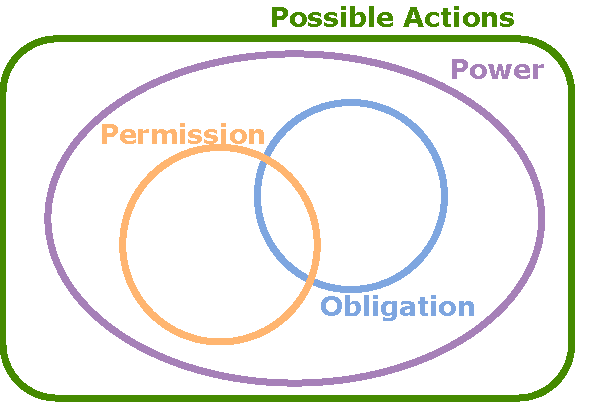
\includegraphics[width=0.6\textwidth]{05_iigo/images/SOMAS_per_obl.pdf}
\caption{Relationship between \emph{power}, \emph{permission} and \emph{obligation}.}
\label{fig:per_obl_sets}
\end{figure} 


For example, the Judge has the \emph{power} to carry out investigations at an IIGO session. There are no rules specifying which specific islands the Judge should investigate. Therefore, the Judge has the \emph{permission} to investigate any `alive' islands during a session. However, the Judge is \emph{obliged} to make at least some number of investigations each turn.



\section{Executive Branch}
\label{sec:executive}
The executive branch is responsible for \textbf{carrying out the law}.
\begin{itemize}
       
    \item The President has the \emph{power} to: 
    \begin{itemize}
        
        \item Select a rule for voting $R^{*}$ to be passed to the Speaker.
        \begin{rule_IIGO}
            The President has the \emph{obligation} to \emph{select} a rule $R^{*}$ if the \emph{rule proposal list} has at least one proposed rule in it.
        \end{rule_IIGO}
        \begin{rule_IIGO}
            The President has the \emph{permission} to \emph{select} a rule $R^{*}$ if and only if $R^{*} \in S$, where $S$ is the \emph{rule proposal list}.
        \end{rule_IIGO}
        
        \item Decide the amount of individual \emph{taxation} (i.e. a specific \emph{minimum} amount of contribution to the common pool for each island) for the current turn.
        
        \begin{itemize}
            \item The President is given the self-reported resource amounts held by each island to assist in this decision.
            %\item Suggested Rule: For any island that has chosen to not report it's resources, the President has the \emph{obligation} to set them an individual tax amount T.
        \end{itemize}
        
        \item Decide the allocation of resources distributed from the common pool to the islands (i.e. a specific \emph{maximum} amount an island is permitted to take from the common pool).
        
        \begin{itemize}
            \item The President is given the \emph{allocation requests} made by each island.
            %\item \emph{}{Suggested Rule:} The President has an obligation to prioritise islands in critical condition.
        \end{itemize}
    \end{itemize}
\end{itemize}



\section{Legislative Branch}
\label{sec:legislative}
The legislative branch is responsible for \textbf{making the law}.
\begin{itemize}

    \item The Speaker has the \emph{power} to:
    \begin{itemize}
        
        \item Call a vote $V$ for a rule $R$.
        \begin{rule_IIGO}
            The Speaker has the \emph{obligation} to \emph{call} a vote $V$ if and only if the President has \emph{selected} a rule $R$ to be voted on.
        \end {rule_IIGO}
        \begin{rule_IIGO}
            The Speaker has the \emph{permission} to \emph{call} a vote $V$ for a rule $R$ if and only if the rule $R = R^{*}$, where $R^{*}$ is the rule \emph{selected} by the President.
        \end {rule_IIGO}
            
        \item Choose which islands are participating in the vote $V$.
       % \footnote{This is our sequential implementation alternative for the power to close the ballot box.}.
        \begin{rule_IIGO}
            The Speaker has the \emph{obligation} to ask for a vote from all alive islands.
        \end {rule_IIGO}
            
        \item Declare the result $C$ of a vote $V$. 
        \begin{rule_IIGO}
            The Speaker has the \emph{obligation} to \emph{declare the result} $C$ for a vote $V$ if and only if the vote V has been \emph{called}.
        \end {rule_IIGO}
        \begin{rule_IIGO}
            The Speaker has the \emph{permission} to \emph{declare the result} $C$ for a vote $V$ if $C = C^{*}$, where $C^{*}$ is the result produced by \emph{calling} the vote $V$.
        \end {rule_IIGO}
        \begin{itemize}
            \item This step is what enables a rule to be \emph{active}.
        \end{itemize}
    \end{itemize}
\end{itemize}




\section{Judicial Branch}
\label{sec:judicial}

The judicial branch is responsible for \textbf{evaluating the law}.
\begin{itemize}
    \item The Judge has the \emph{power} to:
    \begin{itemize}
        \item Perform a number of \emph{inspections}\footnote{An \emph{inspection} \textbf{costs} an expense of resources (See Definition~\ref{def:invst} for more detail).} $I$ and produce a compliance outcome $\mathbb{O}^{*}$\footnote{Note that the compliance outcome $\mathbb{O}^{*}$ considered is a boolean.}.
        %(true: the island has been compliant with the rules in play, false: the island has not been compliant with the rules in play)
        %\begin{itemize}
           % \item For example, to check if the event outcome is \emph{concurrent}\footnote{Again, what is defined as "concurrent"? A clear definition is needed.} with the rules.
        %\end{itemize}
        \begin{rule_IIGO}
            The Judge has the \emph{obligation} to make at least $N$ investigations at each turn.
        \end{rule_IIGO}
        \item Declare the outcome $\mathbb{O}$ of an inspection $I$ to all islands\footnote{This act of broadcasting is especially important for islands to form an opinion about the sanctioned islands accordingly.}.
        \begin{rule_IIGO}
            The Judge has the \emph{obligation} to declare the outcome $\mathbb{O}$ of an inspection $I$ if and only if the inspection $I$ has been performed.
        \end{rule_IIGO}
        \begin{rule_IIGO}
            The Judge has the \emph{permission} to declare the outcome $\mathbb{O}$ of an inspection $I$ if $\mathbb{O} = \mathbb{O}^{*}$, where $\mathbb{O}^{*}$ is the outcome of the inspection $I$.
        \end{rule_IIGO}
        %\item Initiate the removal of the \texttt{President}.
        %\begin{itemize}
            %\item A good Judge would be especially vigilant during \emph{power transfer} regarding the \emph{President} position (see Section~\ref{leg_const} for more detail).
        %\end{itemize}
        \item Invoke economic \textbf{sanctions} (see Section~\ref{sec:sanctions} for more detail).
        \begin{rule_IIGO}
            The Judge has the \emph{obligation} to invoke a sanction $S$ for an island $X$ if and only if an investigation $I$ has an outcome $\mathbb{O}^{*}$ indicating non-compliance, and $I$ is an investigation of an action taken by island $X$.
        \end{rule_IIGO}
        \item Invoke even more severe sanctions in the case of further disobedience to previous sanction(s).
        \begin{rule_IIGO}
            The Judge has the \emph{permission} to invoke a severer sanction $S'$ for an island $X$ if the island $X$ has not fulfilled the requirements of the previous sanction $S$.
        \end{rule_IIGO}
        \item Pardon the islands which are currently sanctioned.
        \begin{rule_IIGO}
            The Judge has the \emph{permission} to revoke any sanction $S$ of an island $X$ at a specific turn.
        \end{rule_IIGO}
    \end{itemize}
\end{itemize}
%(e.g. a new rule that falls under a "sanction" category \hl{[I'm not sure about this being a `new rule` [Ezgi]]}

\subsection{Sanctions}
\label{sec:sanctions}
All sanctions are of economic nature which include:
        \begin{itemize}
            %\item Revoking an island's access to the common pool.
            \item Enforcing an island to contribute a specific amount of resources to the common pool.
            \begin{itemize}
                \item This does not mean that the Judge has the \emph{power} to take resources from an island in order to put them to the common pool -- the island itself is expected to carry out this implication imposed by the sanction itself, otherwise further punishment can be induced by the Judge.
                \item Similarly, \emph{opinion formulation} will follow accordingly whether the island(s) is/are following the implications imposed by the sanction(s).
            \end{itemize}
        
    \end{itemize}
    Sanctions are the associated penalty that comes with an island breaking a specific rule. The Judge is in full control of the penalties associated with breaking any rules. Once the Judge has specified the score of the penalty associated with each time an island breaks a rule, the cumulative penalties accumulated by the island are then used to determine which \textbf{sanction tier} that each island falls into. The score threshold to determine the boundaries of the sanction tiers are set by the Judge. At each turn of the game, each island is told whether they are being sanctioned, and if so, which \textbf{sanction tier} that they are currently in. The \textbf{sanction tiers} of the non-compliant islands are also broadcasted to the other islands in the archipelago. To summarise, the sanctioning process follows these steps:
    
    
    
    %Sanctions are based on an island breaking a rule. Each rule must therefore have an associated penalty. By default, we set these penalties such that they add $1$ to the total sanction score for each island. However, we allow the judge to override this scoring, the judge is able to set their own scores for any particular rule as they desire. This custom scoring is then used when an island breaks a particular rule. By looking at events that occurred in the last turn, and using the customised scoring we provide the holder of the judge role with full control of the penalties for breaking any rules.
    
    





%we then use the cumulative penalties accumulated by each island to determine which Sanction Tier they fall into. The score threshold's required to fall into these sanction tiers is set by the judge and is checked for monotonicity. Each island is told whether they are being sanctioned, and is so what tier they are in. We also tell other islands about which sanction tiers other islands have fallen into. 

    \begin{enumerate}
        \item The Judge has the \emph{power} to set custom penalties associated with breaking any rules.
        \item The Judge is given a list of all events that occurred in the previous turn.
        \item The Judge has the \emph{power} to check whether any, or all of these previous events, involve the islands in the archipelago breaking any rules.
        \item Each of the transgressions is scored using the Judge's custom penalties if the Judge has set them. Otherwise, a score of $1$ is given each time a rule is broken.
        \item The Judge has the \emph{power} to revise the sanction thresholds.
        \item Using the latest sanction thresholds available, each island is assigned to a sanction tier based on the sanction score that it has received.
        \item These sanction tiers are broadcasted to all of the islands in the archipelago.
        \item The Judge then uses sanctions rules in place to calculate the specific amount of resources that each non-compliant island has in order to determine how much it should contribute to the common pool, based on the sanction tier that it is in.
    \end{enumerate}



\section{Constitutional Rights and Obligations in the Archipelago}
\label{sec:const_rights_obl_archi}
Each island has the \emph{power} to:
\begin{itemize}
\item make an \emph{allocation request} (see Definition~\ref{def:alloc_req}) to the President for a specific amount to be allocated to them.
\item report the number of resources it is in possession of to the President.
\begin{rule_IIGO}
    Each island has the \emph{obligation} to report the number of resources it is in possession of to the President.
\end{rule_IIGO}
\begin{rule_IIGO}
    Each island has the \emph{permission} to report the number of resources $R'$ if and only if $R' = R$, where R is the number of resources the island is in possession of.
\end{rule_IIGO}
\item take resources from the common pool.


\begin{rule_IIGO}
    Each island has the \emph{permission} to take at maximum $N$ resources, where $N$ is the specific allocation made by the President to that island\footnote{If no such allocation is made, the island is \emph{permitted} to take any amount of resources.}.
\end{rule_IIGO}
\item contribute resources to the common pool.
\begin{rule_IIGO}
    Each island has the \emph{obligation} to contribute to the common pool an amount greater or equal to that of the individual tax set by the President.
\end{rule_IIGO}
                %The President is in
                %(unless there is a rule in place that dictates how Speaker is to allocate resources).
\item add a rule to the \emph{rule proposal list} (see Definition~\ref{def:rule_prop_list}) at the start of each turn.
        %\begin{itemize}
            %\item The game specification includes how many rules an island can propose each turn.
        %\end{itemize}
        %\item vote  for rules in the Legislative Branch and vote for their favourite islands in elections
\item participate in the legislative branch of the government by casting ballots in votes called by the Speaker
\item vote for an island to be elected for a specific role (e.g. the President, Judge, Speaker) during the elections\footnote{This will be assumed to be true \underline{unless stated otherwise}. %Note that \textbf{diplomatic sanctions} can disable this power of a specific island (see Section~\ref{jud_const}).}.
        }.
\end{itemize}
\section{Accountability Cycle}
\label{sec:accountability}


To ensure that the government avoids corruption and abuse of power, each branch is accountable to another. The President is accountable to the Speaker, the Speaker is accountable to the Judge, and the Judge is accountable to the President (see Figure~ \ref{fig:cycles_in_IIGO}). This accountability cycle is enacted through \emph{monitoring} actions\footnote{Note that the terms \textbf{monitoring} and \textbf{investigation} have similar but quite different meanings in the IIGO context.}. 

The powers related to the accountability cycle and transfer-of-power for each role can be summarized as the following: 
\begin{itemize}
    \item The Speaker has the \emph{power} to: 
    \begin{itemize}
        \item monitor the President.
        \item announce the result of this monitoring.
        \item initiate the transfer-of-power for the Judge.
    \end{itemize}
    \item The President has the \emph{power} to: 
    \begin{itemize}
        \item monitor the Judge.
        \item announce the result of this monitoring.
        \item initiate the transfer-of-power for the Speaker.
    \end{itemize}
    \item The Judge has the \emph{power} to: 
    \begin{itemize}
        \item  monitor the Speaker.
        \item announce the result of this monitoring.
        \item initiate the transfer-of-power for the President.
    \end{itemize}
\end{itemize}

%Unlike investigations performed by the Judge, who performs investigations on island actions in the following turn, each role is given the opportunity to check up on the actions of the role it is responsible for immediately after they have been performed. In this sense, the President can monitor (includes investigative-monitoring) the powers (calling a vote and announcing the result) acted on by the Speaker immediately after the Speaker's announcement (or lack there of). The government officials hold a lot of power so this is to ensure that any wrong-doing is determined as quickly as possible. For this project we are only pursuing one degree of monitoring, that is, the powers relating to the accountability cycle will not be monitored themselves. We assume that agents will act in the interest of themselves and keeping all the islands alive is beneficial to everyone. Hence, while the agents might be inclined to break rules in order to benefit themselves, anyone else breaking the rules is seen as undesirable under the assumption that the system in place is there to benefit all. 


Through the proposed accountability cycle, each role is given the opportunity to check up on the actions of the role it is accountable for immediately after they have been performed. It is clear that the IIGO roles (i.e. the President, Speaker and Judge) hold a considerable amount of \emph{power} in their hands. The accountability cycle is designed to address the possible abuses of this power. With monitoring, any wrong-doing in the IGO is determined as quickly as possible and the role in question can be replaced. 

Within the scope of the coursework, we decided to pursue only \emph{one degree of monitoring}, meaning that the powers relating to the accountability cycle will not be monitored themselves. We assume that agents will act in the interest of all the islands in the archipelago. Hence, while the agents might be inclined to break the rules to benefit in some form, it is assumed that the others will negatively see any non-compliant islands based on the assumption that the proposed IIGO system is in place to maintain the welfare of all the islands.

Let role $X$ be accountable to the role $Y$, which is accountable to the role $Z$. Then:
\begin{rule_IIGO}
$Y$ has the \emph{obligation} to declare the outcome of the monitoring result $M$ associated with the action $A$ undertaken by $X$ if and only if $Y$ has monitored the action $A$ performed by $X$. 
\end{rule_IIGO}
\begin{rule_IIGO}
$Y$ has the \emph{permission} to declare the monitoring result $M$ associated with the action $A$ undertaken by $X$ if and only if $M = M^{*}$, where $M^{*}$ is the outcome of \emph{monitoring} action $A$ performed by $X$\footnote{These constitutional rules should be available to the agents to check their decision against. However, due to having only one degree of accountability cycle in place, these rules are not enforced through any sanctions (i.e. breaking these rules has no consequences as they only deem to be an \emph{agreement} among the roles).}.
\end{rule_IIGO}


\begin{figure}[!htb]
\centering
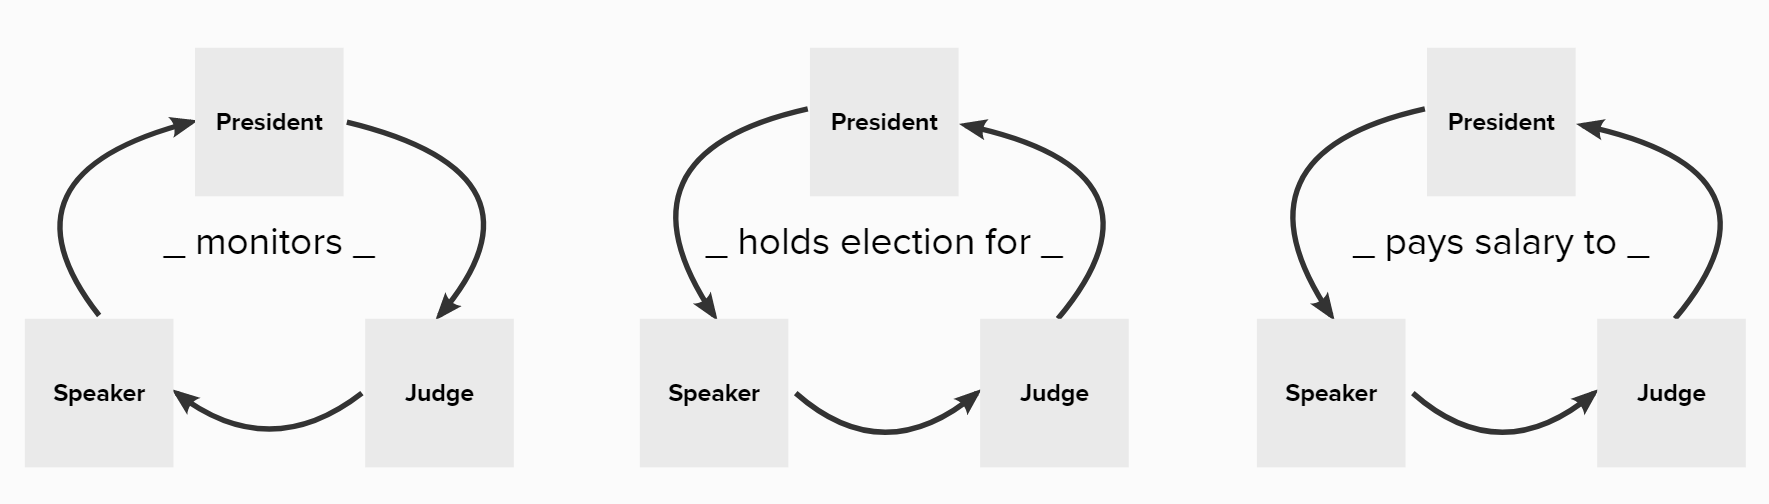
\includegraphics[scale=0.33]{05_iigo/images/role cycles.png}
\caption{Accountability cycle (left), the transfer-of-power cycle (middle) and salary cycle (right).}
\label{fig:cycles_in_IIGO}
\end{figure}


\subsection{Transfer-of-power}
\label{subsec:transfer-of-power}
\begin{enumerate}
    \item The Speaker conducts a vote for the election of the new Judge.
    \item The Judge conducts a vote for the election of the new President.
    \item The President conducts a vote for the election of the new Speaker.
\end{enumerate}
Refer to the Figure~ \ref{fig:cycles_in_IIGO} for further clarification about the transfer-of-power cycle.

\begin{rule_IIGO}
   The role $X$ has the \emph{obligation} to conduct a vote for the election of $Y$ at the end of the term (see Definition~\ref{def:term}) if and only if the role $X$ is accountable to the role $Y$. 
\end{rule_IIGO}.

\section{Budget and Salary}
\subsection{Budget}
%Actions associated with the IIGO have an associated cost that is defined as a configuration parameter. The institutional-power-enabled actions of  identified to require a "computational" component are:

Institutional-enabled-power actions in the IIGO have an associated cost with them. Some examples for such actions include:


%that is defined as a configuration parameter. The institutional-power-enabled actions of  identified to require a "computational" component are:


%We have defined the resource to be an endogenous one, hence any computation surrounding the distribution of the resource must use up some of that resource. 
\begin{itemize}
\item Calling any vote and computing the winner.
\item Declaring (e.g. \textit{announcing} the result of a vote).
\item Setting the amount of \emph{taxation} for each island.
\item Deciding the allocation distribution for each island.
\item Inspecting an island's action history.
\item Monitoring a role.
\end{itemize}

Since IIGO has been designed to act in the common good, IIGO-related costs will be directly withdrawn from the common pool. Since the common pool is considered a communal property of the archipelago, there are rules in place to limit how much each role is allowed to spend in order to perform its own institutional-power-enabled actions. This is the reason why defining the \emph{budget} and keeping it separate for each of the three IIGO roles.


As a role performs institutional-enabled-power actions, the corresponding cost associated with this action is subtracted from the role's budget. A budget of zero means that the role does not have the \emph{power} to perform any of its institutional-power-enabled actions. The removal of the budget rule from the rules in play means the role is allowed to perform as many such actions as it prefers to (as long as those actions are not governed by other rules). 



%As a role performs an endogenous-cost action, the corresponding cost associated with this action is subtracted from the role's budget. Thus, if as a result of an endogenous-cost action a role will be left with negative budget, it will have gone over the budget limit and will have broken the budget rule. A budget of zero means that the role is not allowed to perform any of its institutional-power-enabled actions associated an endogenous-cost. The removal of the budget rule from the rules in play means the role is allowed to perform as many such actions as it pleases (as long as those actions are not governed by other rules). 

The budget rule is also persistent across turns. This means that, assuming nothing else affects the budget, if a role has $100$ resources in its budget at each turn and spends only $10$ resources, this means that this very same role has $90$ resources in its budget at the next turn. On the other hand, islands can choose to increase the budget periodically every turn. This is governed by another budget extension rule.




%one turn and it spends 10, it has 90 resources in it's budget the next turn. 

Finally, it must be noted that the budget is inherently linked with the fact that whether obligations of a specific role can be undergone.
For example, during \emph{monitoring}, it should not be seen as a rule violation if a role has not acted on an obligation if it would go over the budget as a result. 

%This can also be seen as an added clause "... and the action is only permitted if they have the budget" to most rules which govern actions with an endogenous-cost.
%\begin{rule_IIGO}
    %The budget is increased by an amount $N$ every turn.
%\end{rule_IIGO}

%This rule means that, assuming nothing else affects the budget, if a budget is set to increase by 10 resources every turn and the budget is a 100 resources in turn one, the budget is 110 resources in turn 2. Setting this rule to 0 is equal to removing this rule and it means that the budget is never increased. 


\subsection{Salary}
\label{subsec:salary}
A salary is paid to each role in power as an incentive to act in a publicly approved way. %Hence, each role has the \emph{power} to pay a salary to another role following the salary cycle in Figure~\ref{fig:cycles_in_IIGO}.
\begin{rule_IIGO} \label{rule:salary}
   %Each role has the \emph{obligation} to pay the salary of amount $S$ to another if and only if the amount paid $S'$ is equal to $S$.
   Each role has the \emph{obligation} to pay the salary of amount $S$ to one another following the salary cycle in Figure~\ref{fig:cycles_in_IIGO}.
\end{rule_IIGO}

In Rule~\ref{rule:salary}, setting $S=0$ (through changing the active rules in place) means that roles do not have the permission to pay any salary. Removing the Rule~\ref{rule:salary} means that the roles may freely choose the amount $S$ for the salary payments.

\section{IIGO Session order}

\begin{enumerate}
    \item The Judge has the \emph{power} to check the history of actions to confirm whether the previously punished island(s) has/have obeyed the previous round's sanctions, meaning whether they contributed to the common pool accordingly in case of economic sanctions.
    %\begin{itemize}
      %  \item \emph{Suggested Rule:} In case of disobeying sanctions, the Judge is \emph{obliged} and \emph{permitted} to increase the severity of sanctions with respect to specific islands.
   % \end{itemize}
    \item The Judge has the \emph{power} to carry out \emph{inspections} on the history of actions of any island $X$ to check whether:
        \begin{enumerate}
        \item the reported resources of $X$ in the previous round match the real value of resources $X$ had in its private pool for the previous turn.
        \item the island $X$ has retrieved the right amount of the resources from the common pool, based on the \emph{allocation request} evaluated by the previous President.
            \begin{itemize}
            \item An example: In the previous round, the President has decided that the island $X$ can take $Y$ amount of resources from the common pool. If the Judge finds out that the island $X$ has taken an amount of $Y'$ such that $Y' > Y$, the Judge has the \emph{power} to invoke sanctions on the island $X$.
            
            %the Judge is \emph{obliged} and \emph{permitted} to sanction island $X$.
            \end{itemize}
        \end{enumerate}
    \item The Judge has the \emph{power} to invoke sanctions based on the outcome of the inspections.
    \item The President has the \emph{power} to decide to carry out a \emph{monitoring} on:
        \begin{enumerate}
        \item the sanctions imposed by the Judge.
        \end{enumerate}
    \item The islands may report the resources in their private pools to the President.
    \item The President has the \emph{power} to let each island know about the amount of \emph{taxation} they have to pay.
    \item The island has the \emph{power} to make an \emph{allocation request} to the President.
    \item The President has the \emph{power} decide on an allocation of resources and let each island know about the amount of resource allocation they are permitted to take from the common pool.
    \item The island has the \emph{power} to pick and to propose a rule to be voted on to the President.
    \item The President has the \emph{power} to choose a rule to be voted on from the received rule proposals.
    \item The Speaker has the \emph{power} to decide to carry out a \emph{monitoring} on: 
        \begin{enumerate}
        \item the resource allocation decided by the President.
        \item the rule proposed by the President.
        \end{enumerate}
    \item The Speaker has the \emph{power} to call a vote.
        \begin{enumerate}
        \item The islands vote in support of, or against, the rule (aye or nay) anonymously.
        \end{enumerate}
    \item The Speaker has the \emph{power} to announce a result of a vote to the islands and carries out the law change, if required (e.g. deleting/rejecting a rule if there is a majority nay vote).
    \item The Judge has the \emph{power} to decide to carry out \emph{monitoring} on:
        \begin{enumerate}
        \item the vote called by the Speaker.
        \item the Speaker announcing the result.
    \end{enumerate}
    \item The roles pay salary for one another following the accountability cycle in Figure~ \ref{fig:cycles_in_IIGO}.

\end{enumerate}



\section{Future Work}

\begin{itemize}
    \item \textbf{Diplomatic sanctions}: Although having the potential of being a good alternative for severer sanctions discussed in  Section~\ref{sec:sanctions}, diplomatic sanctions are \emph{not} implemented within the scope of the coursework. \\
    Suggested diplomatic sanctions include:
        \begin{itemize}
            \item Revoking an island's eligibility to vote and to be elected for a position.
            \item Revoking an island's eligibility to propose a rule/motion.
        \end{itemize}
    \item \textbf{Immutable rules}: Within the scope of the coursework, a subset of rules could have been categorised as immutable. This means that to change such immutable rules, the islands first need to vote to change their status to be \emph{mutable}, and consequently, hold another vote to change these mutable rules.
    %\item \textbf{Adding rules to the proposal list: } 
\end{itemize}

    \chapter{Game Design}

\section{Implementation}
\label{sec:GD:implementation}

Implementation design was important as the majority of the class were involved in writing simulation code. As such, dedicated \emph{infrastructure} engineers from each team were elected to form an infrastructure team responsible for building the central part of the game, otherwise known as the \emph{server}. Each team's infrastructure engineer was tasked to own the implementation of a slice of the server.

One such sub-team was the \textbf{core} infrastructure team, responsible for building the core parts of the game server. Inputs were taken from the entire class to choose the best implementation strategies and design--a solid and simple core foundation was paramount to allow clean continuous integration of code and ideas from all contributors. The subsections below detail implementation specifics of the game's simulation.

\subsection{Architecture}
\label{sec:GD:implementation:arch}

The structure of the game was closely modelled after a \emph{client-server} model\footnote{\url{https://en.wikipedia.org/wiki/Client-server_model}}, but note ``closely''--whilst the nomenclature was taken directly from the aforementioned model, there are some differences. \emph{Server} and \emph{client} in this context bear the following definitions:

\begin{definition} \label{def:server}
    The \textbf{server} is the central game runner, responsible for initiating game events (such as a disaster or the start of a turn). Certain events require the actions of agents, in which the server will invoke a function on the agents to receive a response. Further, the server acts as a source-of-truth for the game's state.
\end{definition}


\begin{definition} \label{def:client}
    Each \textbf{client} is implemented by an agent. The client provides an interface of functions in which the server can invoke. Moreover, clients may also invoke certain functions from the server's interface to read specific game information.
\end{definition}

The major difference of this architecture to a traditional client-server model is that, in the former, the stateful central server drives the other clients (by triggering events and eliciting responses), as opposed to clients sending stateless requests to a server to receive a response in the latter. Furthermore, whilst the client and server have been separated architecturally, the entire system still operates as a single process.

\subsection{Technology Stack}
\label{sec:GD:implementation:techstack}

Agreeing on a technology stack proved to be challenging--the class had varying levels of programming expertise. Whilst Prolog\footnote{\url{https://en.wikipedia.org/wiki/Prolog}} and Qu-Prolog\footnote{\url{https://staff.itee.uq.edu.au/pjr/HomePages/QuPrologHome.html}} (an extension to the former) were used to cover topics in the lectures, the class did not favour them over more well-known and established imperative programming languages. Hence, time was dedicated to formulate a consensus to decide on the technology stack, with primary focus given on the choice of implementation language. Firstly, high priority requirements were defined for the stack:

\begin{itemize}
    \item Easy to learn
    \item Easy to setup
    \item Cross-platform
    \item Easily maintainable
    \item Friendly features
\end{itemize}

Minimum Working Examples (MWEs) comprising a single server and two clients were created in different stacks, which served as starting points for discussion among members of the class. The MWEs implemented are as follows.

\begin{enumerate}
    \item \textbf{Multi-language}\footnote{\url{https://github.com/SOMAS2020/somas-demo}}.
          A multi-language (C++ server with a Python and a C++ client) MWE was first set up. It was first thought that allowing agent teams to choose the programming language they were most familiar with would speed up development. However, despite this stack's benefits, it could not be easily made cross-platform. Each agent's code would need to be run in a separate process, and Inter-Process Communication (IPC) would be required to pass messages. IPC is quite low-level and varies vastly among different systems. Further, protocols for the IPC would also need to be set up to pass the correct message, and having no strong typing as in a strongly-typed language (or session-typed\footnote{\url{https://arxiv.org/abs/1906.03836}}) approach would make it difficult to maintain and develop.

    \item \textbf{Python}\footnote{\url{https://github.com/SOMAS2020/somas-demo-py}}.
          Python\footnote{\url{https://www.python.org/}} is widely used by the scientific community in recent years with the growing ubiquity of scientific computation packages available for it. As such, Python was a strong contender as most of the class already know Python from past projects. However, Python's weak typing meant it scored low on the ``easily maintainable'' part--the server and client interfaces would benefit a lot from strong typing. While add-on static typing tools such as \texttt{mypy}\footnote{\url{https://mypy.readthedocs.io/}} could be employed (it is also used in the MWE), it would still not be as powerful as built-in strong typing as in languages such as C\# and Go.

    \item \textbf{C\#}\footnote{\url{https://github.com/SOMAS2020/somas-demo-cs}}.
          C\#\footnote{\url{https://docs.microsoft.com/en-us/dotnet/csharp/}} is the flagship language of the .NET ecosystem. C\# shares a large part of its design to the more popular C++. C\# is strongly-typed, and promotes use of clean Object-Oriented Programming (OOP). Many of the features from C/C++ that can be \emph{dangerous} are not present or hidden, making it more beginner friendly. A drawback is that some experience with C-family languages is required to pick up C\# quickly.

    \item \textbf{Go}\footnote{\url{https://github.com/SOMAS2020/somas-demo-go}}.
          While most of the class was not familiar with Go\footnote{\url{https://golang.org/}}, its simple language syntax and highly-featured toolchain make it very easy to learn. The modern Go toolchain makes it extremely simple for programs to work cross-platform. While Go's omission of OOP and generics might be seen as a disadvantage, it makes it an easy language to learn, and prevents pitfalls commonly caused by such ``features''. Go, like C\#, is strongly typed. Moreover, Golang's great support for WebAssembly\footnote{\url{https://webassembly.org/}} would prove useful for visualisations, further detailed in~\ref{sec:GD:implementation:visualisations}. Another nice feature is that concurrency can be easily implemented in Go, which meant that agent actions could be run concurrently to speed up simulations.
\end{enumerate}

After discussion, scores (out of 10) were given for each stack. Table~\ref{table:techstackscores} shows these scores. The multi-language and Python approaches were removed from consideration--the former due to its low total score and the latter because of its low maintainability. The decision between C\# and Go was harder, and ultimately resulted in a \emph{simple majority} vote by the class. 37 people voted in total, with 25 in favour of Go. Hence, Go was finally chosen.

\begin{table}[h]
    \centering
    \caption{Scores given for each stack based on requirements}
    \label{table:techstackscores}
    \begin{tabular}{|c|c|c|c|c|c|c|}
        \hline
        Stack                     &
        \makecell{Easy              \\ to \\ learn}              &
        \makecell{Easy              \\ to \\ setup}              &
        \makecell{Cross-platform} &
        \makecell{Easily            \\ maintainable}             &
        \makecell{Friendly          \\ features}                 &
        \makecell{Final             \\ score \\ (out of 50)}
        \\
        \hline
        Multi-language            &
        6                         &
        2                         &
        0                         &
        2                         &
        10                        &
        20
        \\
        \hline
        Python                    &
        8                         &
        6                         &
        8                         &
        3                         &
        8                         &
        34
        \\
        \hline
        C\#                       &
        6                         &
        5                         &
        8                         &
        9                         &
        8                         &
        37
        \\
        \hline
        Go                        &
        8                         &
        8                         &
        10                        &
        8                         &
        6                         &
        40
        \\
        \hline
    \end{tabular}
\end{table}


\subsection{Visualisations}
\label{sec:GD:implementation:visualisations}

\subsubsection{Toolchain}
A benefit from the choice of the Go technology stack was that it supports compiling source code into WebAssembly out of the box. WebAssembly can be run efficiently in most modern browsers, which meant that in-browser simulations can be run and then visualised on a website.

The website (\url{https://somas2020.github.io/SOMAS2020/}) features... % TODO:- Vis team: yp717 et al.

\subsection{Engineering Practices}
\label{sec:GD:implementation:practices}

Developing and maintaining a codebase with contributions from around 40 developers was projected to be non-trivial. Therefore, good software engineering practices and rules were employed to be upheld by all contributors to make the process smoother and--where possible--automated.

\subsubsection{Code testing}

While Go is strongly typed and would mean that most errors can be detected at compile-time (or even at time of coding with its performant language server), having unit and integration tests greatly improved the maintainability and ease of development of the project--these issues were particularly important as this was a large-scale group software engineering project--developers stepping on each other's toes is a common occurrence in non-tested group project code. Henceforth, tests were required for non-trivial server-side code.

\subsection{Peer Review}

Peer review was also setup via GitHub pull requests--each change required the approval of another member in the infrastructure team. This practice not only promoted consistent code design and implementation, it minimised mistakes and ensured that the code implementation meets design and implementation requirements set forth. Further, as there was variation in programming skill among code contributors, knowledge sharing was facilitated by code reviews. This was also a critical opportunity for engineers to learn more about the other code being contributed to the project.

\subsection{Continuous Integration}
\label{sec:GD:implementation:practices:CI}

Via GitHub Actions\footnote{https://github.com/features/actions}, continuous integration was set up. Each Pull Request (PR) was set up to trigger automated runs of written tests and a full simulation in addition to static code analysers such as linters. These checks must all pass for the PR to be merged into the main branch. Automated testing and code analysis saved time and facilitates regression testing, as all tests--existing and new--were run for each change. Running a full simulation also served as a good stress-test for the system to make sure that it does not crash on a similar full simulation. Further, automated tests were run on a reference system (Ubuntu 20.04 with Go 1.15.5 and Node 14), helping to prevent system-specific quirks or bugs from polluting the codebase.

\subsection{Continuous Development}

On receiving PR approval, passing automated tests and finally merging into the main codebase, the visualisation website is automatically rebuilt with the latest changes. This saved time as manual builds were not required. The builds were produced on a reference system (identical to that mentioned in~\ref{sec:GD:implementation:practices}), ensuring consistent builds free from system-specific quirks. Further, automated builds meant that the website always runs on the latest codebase.

    \chapter{Environment}
\section{Foraging}
\subsection{Foraging Background}

Foraging is a base requirement that is needed as it is a method of obtaining more resources from the starting amount.Foraging is based on the concept of inputting resources to get a return.\\

\subsubsection{Underlying concept}
The goal of foraging in this “game” is to introduce a certain dilemma to the agents to further understand the behaviours of multiple (6) intelligent agents working together to reach a goal with different personal goals. By having 2 methods of foraging it introduces the concept of decision making between the islands allowing for strategic interactions to maximise personal benefits whilst still reaching the overarching goal of survival.\\  

The inspiration for our concept of foraging comes from the stag hunt game furthermore it introduces elements from it. Specifically it brings in the concept of \textbf{no dominant strategy} and how \textbf{ one agents choice can impact other agents.}\\

The concept of stag hunt is that each player selects a method of hunting and if they differ then the social welfare (total payoff) is significantly less than if they both go stag hunting. The selection of stag means the agent is going for higher \textbf{payoff}whilst the selection of hare indicates that the agent is going for \textbf{risk aversion} as both agents are required to stag hunt to get any personal welfare. \\

\subsubsection{Modifications to the original concepts} 
A few changes have to be made to make this dilemma viable for our multi-agent system, in addition to adding realism. 

\begin{enumerate}
    \item Changed the dependency to be based on the input resources rather than the number of islands participating. This added a more realistic element to the dilemma as in reality a hunt’s return would be based on the amount of resources (people, food, water and materials) entered rather than the number of islands participating.
    \item Instead of a specified return we have a probabilistic return which adds a randomness element to the game to prevent pattern recognition. These probabilities can be tied to the population, disasters, forecasting and number of animals hunted.  
\end{enumerate}

\newpage
\subsection{Functions within Foraging}
\subsubsection{Inputs, outputs and Parameters}

This is an element implemented in the code base. It determines the method of foraging, which is either deer hunting being payoff focused or fishing being risk aversion.\\


\subsubsection{Primary Code Function}

\begin{table}[h]
\begin{center}
\begin{tabular}{|p{1.5in}|p{1.5in}|p{1.5in}|} \hline
\textbf{Functions} & \textbf{Inputs} & \textbf{Outputs} \\ \hline
\texttt{TotalInput} & -Island Number\newline -Foraging amount & -Total foraging amount \\ \hline
\texttt{deerUtilityTier} & -Total foraging amount\newline -Maximum deer per hunt\newline -Decay value & -Tier (according to input resources) \\ \hline
\texttt{deerReturn} & -Bernoulli's probability\newline -Exponential decay & -Weight of the deer (0 if deer was not caught) \\ \hline
\texttt{Hunt} & -Tier\newline -Weight of deer & -Utility (cumulative sum of the weight of the deers) \\ \hline
\end{tabular}
\caption{\label{tab:table-name}Foraging Deer Hunt Method's main functions}
\end{center}
\end{table}

\subsubsection{Tier System}

The deer hunting and fishing is divided into tiers (the number of fish that can be caught in a given day) which depends on the total input resources. Where the “zero” tier represents the cost of getting to the hunting location.\\ 

Beyond the zero tier we have the cost of catching another deer/fish, which decreases as it is easier to catch the second animal than the first since we have already arrived at the hunting location. It should be noted there is a limit to how many animals we can catch in a given day.\\

The focus of fishing is to avoid risk at the expense of payoff. Thus all the tier requirements are lower than the deers however the return is also lower, in addition to this the “zero” tier has been removed. Thus, if only 1 island goes fishing they are still expected to have a low return as long as they have enough resources to catch the first fish. \\

The focus of deer hunting is higher payoffs therefore it has better returns but all of its tier thresholds are significantly higher and it also has a “zero” tier. Therefore it is possible for a single island to go deer hunting without enough resources to reach the hunting location leading to no return.

\begin{equation}
Increments\ of\ catching\ n\ deer's=
\left( \begin{array}{ll@{}}
n=0 -> \Delta^0 = 1 \\
n=1 -> \Delta^1 = 0.8^1 \\
n=2 -> \Delta^2 = 0.8^2 = 0.64 \\
n=2 -> \Delta^3 = 0.8^3 = 0.512 \\
n=4 -> \Delta^4 = 0.8^4 = 0.4096\\
\end{array} \right) 
\end{equation}

\begin{equation}
Cumulative\ deer \ cost \sum_{n=0}^{n} \Delta^{n} = \Delta^{0} + \Delta^{1} + \Delta^{2} + \Delta^{3} + \Delta^{4} + ....
\end{equation}

\begin{equation}
Cumulative\ fishing\ cost \ = \ \sum_{n=1}^{n} \Delta^{n} = \Delta^{1} + \Delta^{2} + \Delta^{3} + \Delta^{4} + \Delta^{5} + ....
\end{equation}

Equations that show the formulation of the decay function for tier system.\\

The tier system is shown above, where n stands for the tiers, with decay costs ($\Delta$) of 0.8 for both the deer hunt and fishing. Fishing cost starts at n=1 due to the reduced cost.\\

\begin{figure}[!htb]
    \centering
    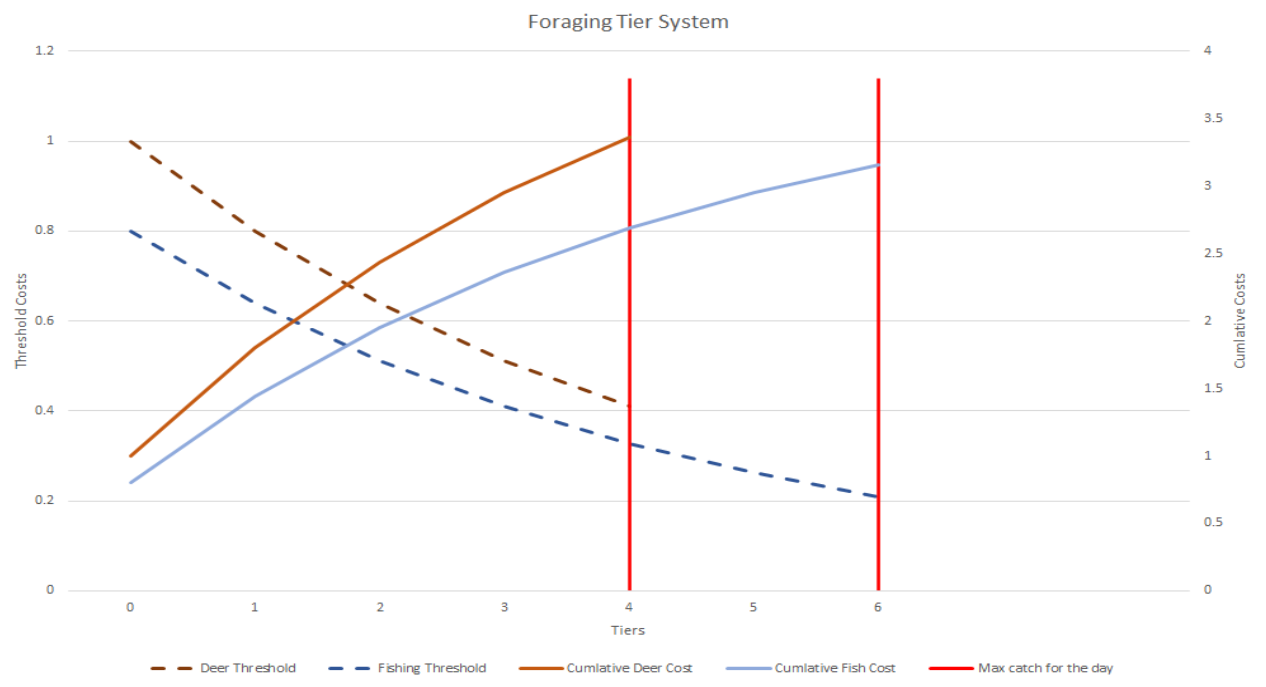
\includegraphics[width=0.9\textwidth]{04_environment/Images/Foraging Tier System.PNG}
    \caption{Foraging Tier System}
    \label{Images:Foraging Tier System}
\end{figure}

As the tiers increase the cost per animal decreases but the total cost increases up to a daily catch limit. Thus if teams collaborate, they could invest less as individuals to get a good return through deer hunting, however if they invest too much then they will over spend as they reach the daily max catch. Thus it would be beneficial for some teams to go fishing which has a higher maximum catch per day but comes with lower returns (thus there is a need for some self sacrifice to be done to reach maximum welfare). \\ 

Fishing has similar functions with the key difference being the Tiers start at 1 and Normal distribution. \\

\newpage
\subsection{Examples Distributions}
\subsubsection{Example of the distribution for foraging return (Deer hunting - payoff dominant)}

\begin{figure}[!htb]
    \centering
    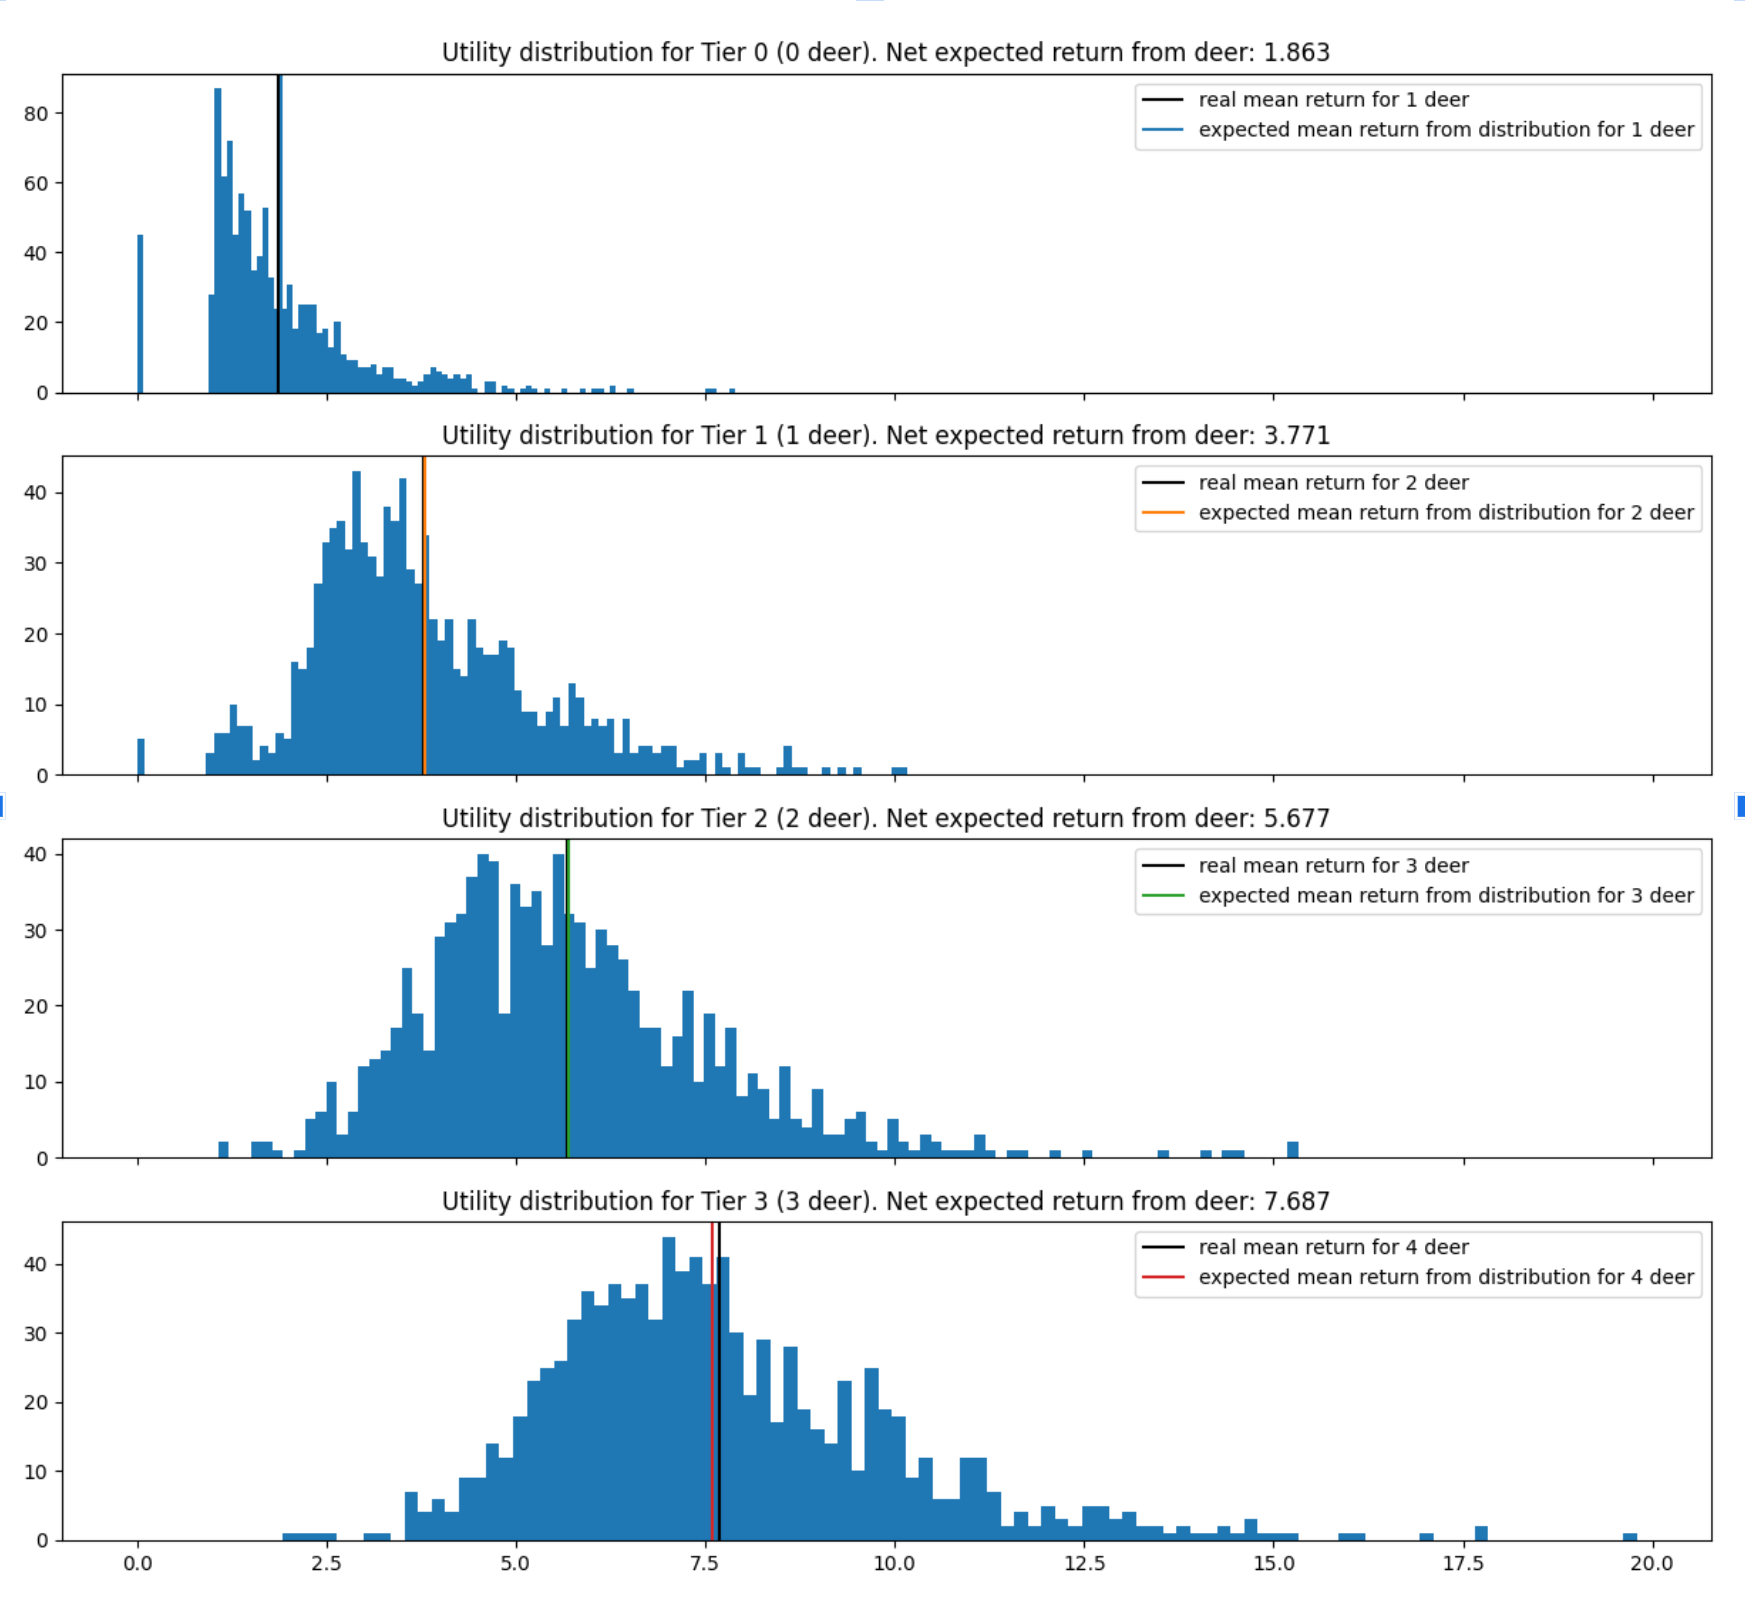
\includegraphics[width=1\textwidth]{04_environment/Images/Distribution of Foraging returns Deer Hunting.PNG}
    \caption{Deer hunting payoff dominant Distribution for foraging return}
    \label{Images:Distribution of Foraging returns Deer Hunting}
\end{figure}

To increase the risk we have used a Bernoulli Random Variable (D) that makes it possible for the hunt to not return any resources. Whilst the Exponential Decay (W) is to disincentive too much resources being placed in hunting and hoping for a high return. However this all comes with the benefit of significantly higher (2x) returns than fishing.\\ 

The above graph represents the return utility which represents the return multiplier of the foraging. The average \textbf{expected mean} return across 1000 iterations is shown by the colourful lines which is close to the \textbd{real mean}.\\

\newpage
\subsubsection{Fish hunting - risk aversion}

Fishing is similar to Deer hunting, except that it uses only a Normal Distribution (F), which focuses on avoiding risk by being very predictable and safe. The Figure below illustrates the return utility function of fishing.\\

\begin{figure}[!htb]
    \centering
    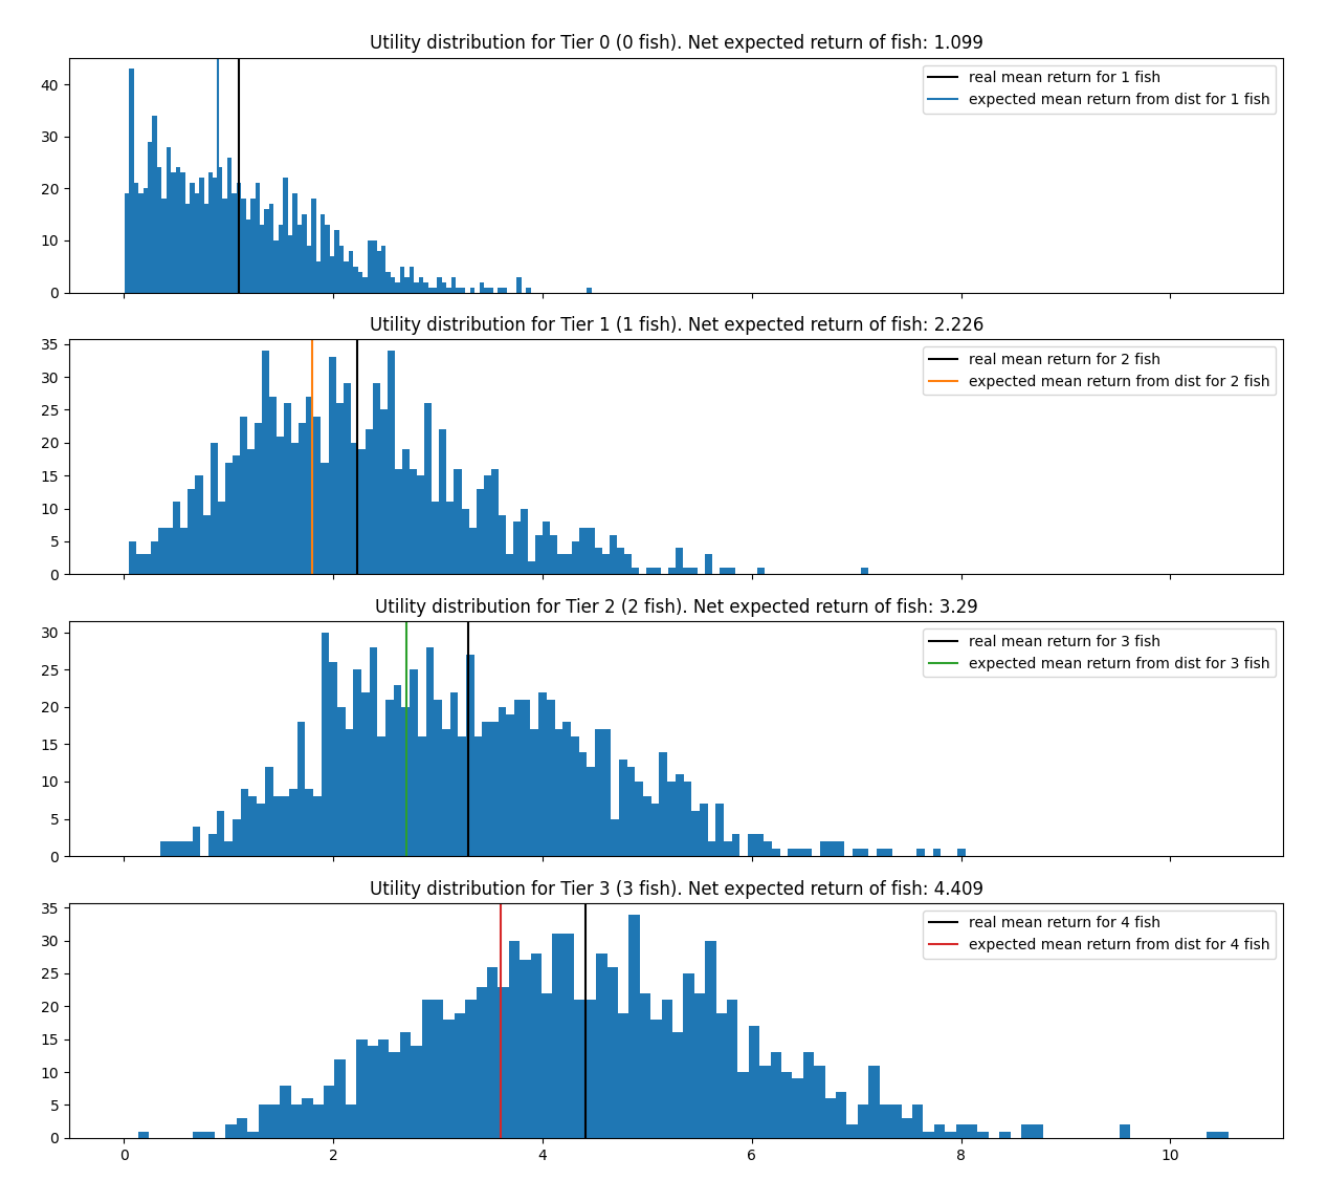
\includegraphics[width=1\textwidth]{04_environment/Images/Distribution of Foraging returns Fishing.PNG}
    \caption{Fishing Risk aversion Distribution for foraging return}
    \label{Images:Distribution of Foraging returns Fishing}
\end{figure}

As seen in the graphs the return for the deer is almost double that of the fish return whilst the fish return is much easier to obtain due to the lower cost of catching fish. \\

\newpage
\subsection{Solution Concepts}
\subsubsection{Dominant Strategy}

In our implementation there is no dominant strategy as picking deer hunt when other players switch to fishing could lead to significantly worse returns due to insufficient resources. Whilst picking fish hunt when enough resources are invested in deer hunting will net you a worse return than if you went deer hunting.\\

\subsubsection{Nash Equilibrium}

In the regular stag hunt game there are 2 pure Nash equilibria, where both players go for either payoff or risk aversion. In our implementation there are multiple Nash Equilibria; these would be the points where the islands cannot benefit themselves by moving to deers hunting to generate more return. As there is a limit to how many deers that can be hunted thus by moving to deer hunting they are getting a worse return than if they just stayed at fishing. Whilst the islands at the deer hunt are already making a greater return and have no reason to switch to fishing.\\ 

\subsubsection{Pareto Optimal Strategy}

At some point all players will be in a position where changing foraging methods will not yield any better income for themselves and in fact also hinder others. This is due to the max daily deer hunt limit which will create a maxim return on the deer hunt. Therefore there will be points where the islands will change as the amount of resources being entered into both methods of foraging is the most efficient, this being where deer returns are maximised. There may also be a point where the user can benefit by switching away from deer hunting, however this will cause the other islands in the deer hunt to have a worse pay off due to a possible drop in tier resulting in worse returns.\\

\begin{figure}[!htb]
    \centering
    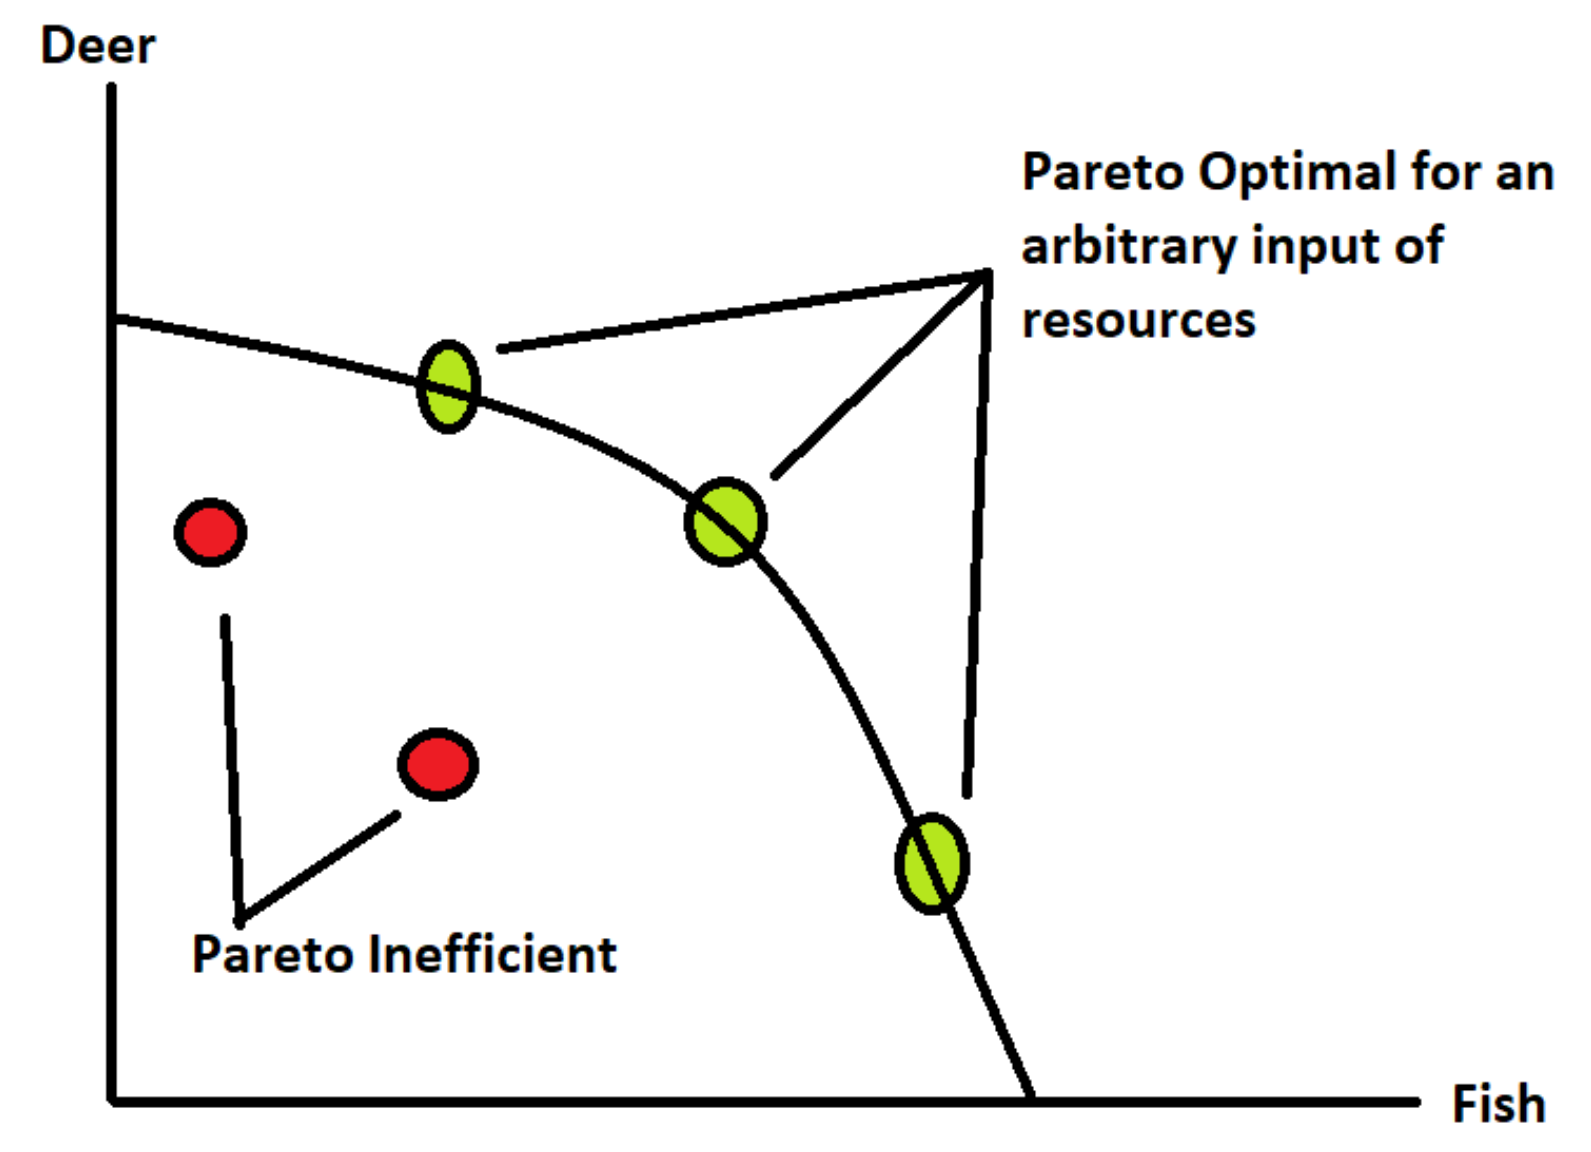
\includegraphics[width=0.7\textwidth]{04_environment/Images/Pareto Optimal Strategy.PNG}
    \caption{Pareto Optimal Strategy}
    \label{Images:Pareto Optimal Strategy}
\end{figure}

\subsubsection{Social Welfare Maximisation}

It is possible for these islands to find the social welfare maximum in this foraging function with enough time. The islands could identify the exact amount of resources needed, for both fishing and deer hunting, to achieve the best return according to the maximum number of animals. Thus by cooperating who goes where and spends how much they are able to maximize their returns without spending more resources than necessary.\\

\subsection{Extended Work}

For the future implementations, our additions focus on further exploring the dynamics of our agents and allowing for a more complex decision-making interaction between clients and the environment. Some of these design ideas were later implemented in self-organising multi-agent system and others are expressed for the sake of completeness and future work recommendations.\\

Some changes have been made to make foraging more volatile and unpredictable. These will add to the complexity of the system, allowing the teams to further evaluate the clients’ performance on observing and using learned knowledge to take action.\\

\subsubsection{Incorporated Changes: Population density}

Introducing a model that controls the population density of deer allows us to increase the complexity of the foraging function. In short, the deer hunting capacity decreases with decreasing population and increases with an increasing population. This will then influence the maximum deer per hunt parameter(n), which in turn results in a more complex return calculation function (\texttt{\textbf{DtotalReturn}}), which would make it harder for agents to figure out forage tier boundaries to optimise their strategies.\\

The population change can be dynamic depending on various environmental factors, fetched from the rest of the system. For example, a Disaster could supposedly cause the population density of deer to halve, making it harder to forage and therefore, causing lower returns. For future implementations, the team uses a single species population model and more specifically logistic modelling for the deer and fish population. The model can be described in the equation below.\\

\begin{equation}
\frac{\mathrm{d} P}{\mathrm{~d} t}=k(N-P)
\end{equation}

\begin{itemize}
        \item “P” is the total Population \item “N” is the maximum deer/fish population (“carrying capacity” formally)
        \item “k” is the growth coefficient
        \item “t” is time
    \end{itemize}

In our implementation \textbf{“k”} and \textbf{“N”} are constants but it would be interesting to see what would happen if we were to increase the growth coefficient, causing a population growth and observing the islands’ dynamics. Will they keep on “investing” higher resources each turn, taking advantage of the deer/fish abundance, or will they stick to their original, safe and static strategy?\\

Below, we can see a simulation of the implemented logistic model, with a growth coefficient of 0.2 and \textbf{“N”} of 8. It can be seen that overtime there is an unpredictable pattern to population changes, which would be interesting to see affecting the tier system and in extend, the deer/fish foraging strategies of the agents.\\

\begin{figure}[!htb]
    \centering
    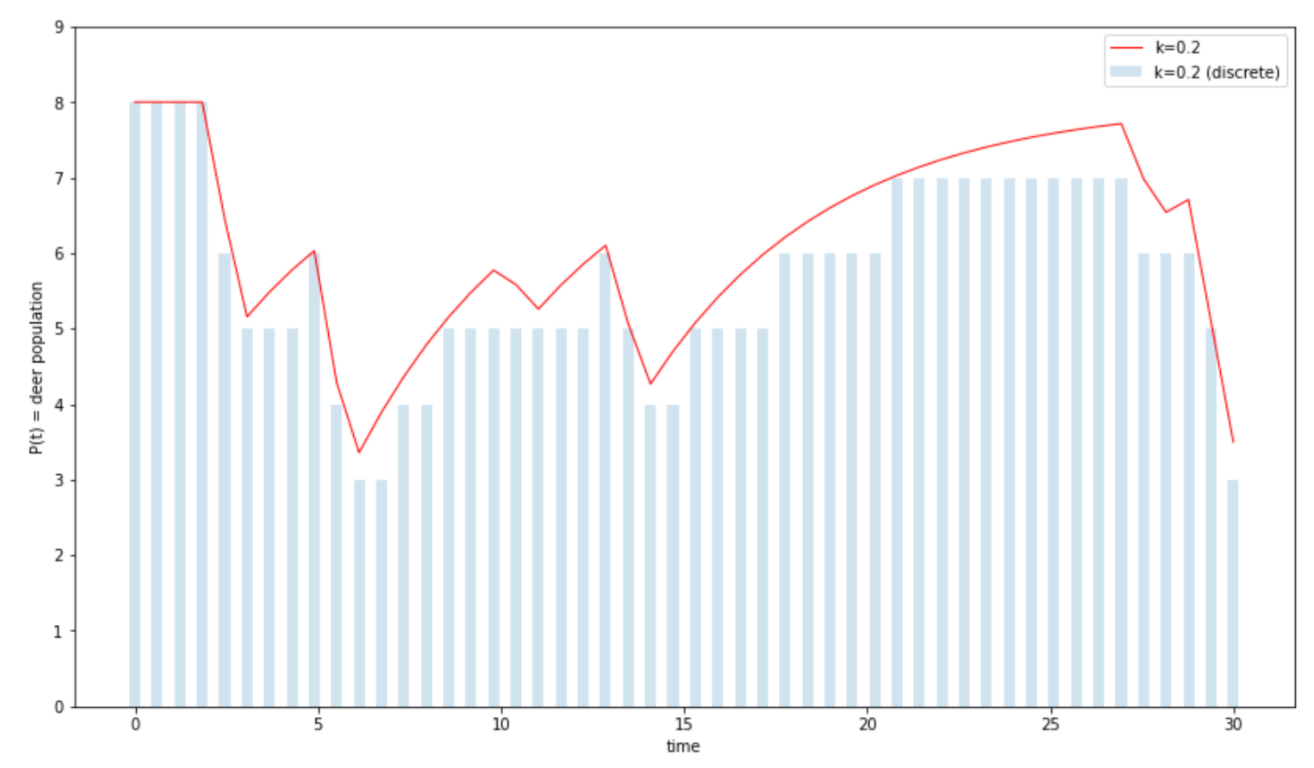
\includegraphics[width=1\textwidth]{04_environment/Images/Deer population over time.PNG}
    \caption{Deer population over time (turns) under Logistic modelling with a growth coefficient of 0.2.}
    \label{Images:Deer population over time}
\end{figure}

Modelling the population (or linking it to other environmental elements) allows us to make sure that the system’s dynamics are varying, making it harder for islands to settle onto a single foraging method because it always results in better returns. Pareto optimality is therefore harder to achieve and thus maximising social welfare is trickier, requiring agents to make more informed decisions, recognizing possible patterns. Of course, that would be an easier task for the islands, if they had knowledge on what is affecting the population (i.e. disasters), whereas a logistic model function might be more abstract in the eyes of our agents, requiring more processing. \\

\subsubsection{ Incorporated Changes: Method of resource allocation}

Lastly, in future implementations, a parameter can be set that allows either an equal split of returns after foraging no matter the input, or a proportional split that is dependent on the amount of resources inputted by each island. Both of these implementations work in accordance to the previous specification. Such change will allow us to observe the concept of free-riding further, looking at how greedy islands behave in the case of uniform resource returns. Will the islands seek to minimise inputs and benefit from the more generous islands, even at the cost of being allocated a lower tier? Will they input just enough to maximise the tier they are foraging in? Or, will they observe other island’s previous contributions and make a decision based on that? These are some of the questions we can later explore using this future change. \\

\subsection{Future Work Concepts}

For the Future implementations, our additions focus on further exploring the dynamics of our agents and allowing for a more complex decision-making interaction between clients and the environment. Some of these design ideas were later implemented in self-organising multi-agent system and others are expressed for the sake of completeness and future work recommendations.\\

Some changes have been made to make foraging more volatile and unpredictable. These will add to the complexity of the system, allowing the teams to further evaluate the clients’ performance on observing and using learned knowledge to take action.

\subsubsection{Incorporated Changes: Population density}

Introducing a model that controls the population density of deer allows us to increase the complexity of the foraging function. In short, the deer hunting capacity decreases with decreasing population and increases with an increasing population. This will then influence the maximum deer per hunt parameter(n), which in turn results in a more complex return calculation function (\texttt{\textbf{DtotalReturn}}), which would make it harder for agents to figure out forage tier boundaries to optimise their strategies.\\

The population change can be dynamic depending on various environmental factors, fetched from the rest of the system. For example, a Disaster could supposedly cause the population density of deer to halve, making it harder to forage and therefore, causing lower returns. For future implementations, the team uses a single species population model and more specifically logistic modelling for the deer and fish population. The model can be described in the equation below.\\

\begin{equation}
\frac{\mathrm{d} P}{\mathrm{~d} t}=k(N-P)
\end{equation}

\begin{itemize}
        \item “P” is the total Population \item “N” is the maximum deer/fish population (“carrying capacity” formally)
        \item “k” is the growth coefficient
        \item “t” is time
    \end{itemize}

In our implementation \textbf{“k”} and \textbf{“N”} are constants but it would be interesting to see what would happen if we were to increase the growth coefficient, causing a population growth and observing the islands’ dynamics. Will they keep on “investing” higher resources each turn, taking advantage of the deer/fish abundance, or will they stick to their original, safe and static strategy?\\

Below, we can see a simulation of the implemented logistic model, with a growth coefficient of 0.2 and \textbf{“N”} of 8. It can be seen that overtime there is an unpredictable pattern to population changes, which would be interesting to see affecting the tier system and in extend, the deer/fish foraging strategies of the agents.\\

\begin{figure}[!htb]
    \centering
    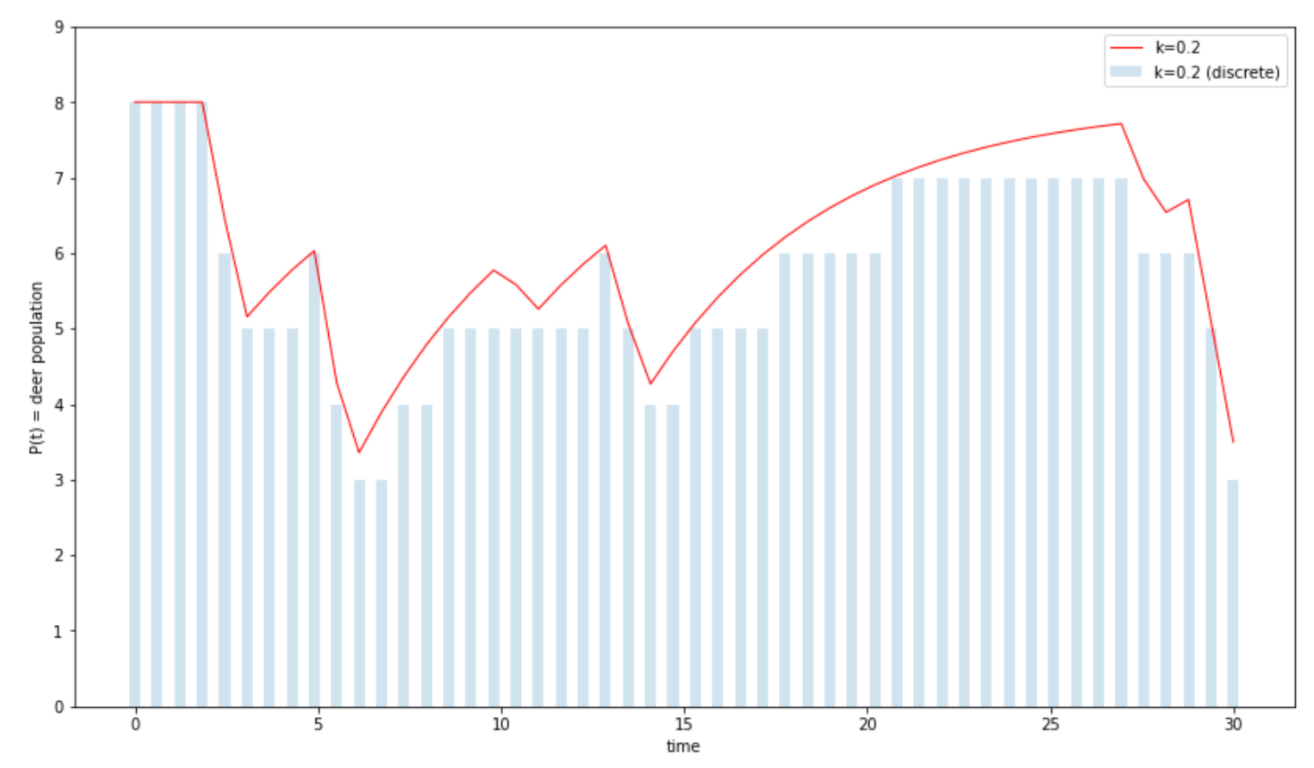
\includegraphics[width=0.8\textwidth]{04_environment/Images/Deer population over time.PNG}
    \caption{Deer population over time (turns) under Logistic modelling with a growth coefficient of 0.2.}
    \label{Images:Deer population over time}
\end{figure}

Modelling the population (or linking it to other environmental elements) allows us to make sure that the system’s dynamics are varying, making it harder for islands to settle onto a single foraging method because it always results in better returns. Pareto optimality is therefore harder to achieve and thus maximising social welfare is trickier, requiring agents to make more informed decisions, recognizing possible patterns. Of course, that would be an easier task for the islands, if they had knowledge on what is affecting the population (i.e. disasters), whereas a logistic model function might be more abstract in the eyes of our agents, requiring more processing. \\

\subsubsection{ Incorporated Changes: Method of resource allocation}

Lastly, in future implementations, a parameter can be set that allows either an equal split of returns after foraging no matter the input, or a proportional split that is dependent on the amount of resources inputted by each island. Both of these implementations work in accordance to the previous specification. Such change will allow us to observe the concept of free-riding further, looking at how greedy islands behave in the case of uniform resource returns. Will the islands seek to minimise inputs and benefit from the more generous islands, even at the cost of being allocated a lower tier? Will they input just enough to maximise the tier they are foraging in? Or, will they observe other island’s previous contributions and make a decision based on that? These are some of the questions we can later explore using this future change. \\

Further work could be done to make sure that there is enough complexity to explore the dynamics of our agents. Due to the project’s time constraints, some interesting ideas were not implemented but were thoroughly examined during the design process.\\

An important add-on to our previous implementation could be the enforcement of laws by the IIGO for the number of islands that can go foraging. That would introduce the need of internal client relationships, adding another level of decision-making complexity to the agents. The specific alteration could result in some interesting findings. For example, there could be an auction scenario where islands would bid with their input resources, where only the highest bidders would be able to forage, as limited by the IIGO. Therefore, Islands with the lowest resources would be out-bidded, possibly causing a long-term resource depletion that would need to be mitigated by the more resourceful islands later in the game. It would be interesting to see how such change would affect the free-rider problem and how islands would adjust their strategies to out-bid other islands.\\

Another change that could be made, is to let islands choose who they can forage with. That could be in the form of direct messaging or voting. Essentially, our speculation is that agents would avoid the free-riding problem in both cases by enabling agents to make collective decisions based on communicated resource contributions. That’s because free-riders would be out-voted or not invited for foraging. That, in combination with the aforementioned tier system, would possibly result in all the islands contributing as much as possible to the input foraging “pool”.  However, it would be interesting to see if islands can then reach Pareto optimality, where every single agent gets the best possible return for their input.\\

In addition to the above suggestions, area limited foraging where agents would only be allowed to forage with only one neighbouring island using a ranking algorithm. This could also be enforced and implemented in a future iteration. Moreover, this particular scenario could be extended by programming prey densities to be geofocused, where prey populations could vary between regions on the “map”. Islands would then need to make a strategic plan on how their ranking of neighbouring islands would change in accordance to their returns and returns broadcasted from other island pairs.\\

Finally, more foraging options could be added in future implementations. For example, a third foraging technique, call it whale it hunting, could be created. That would have an even higher return than the deer hunting, deeming it an appealing forage method. The barriers of entry could be similar to that of the deer hunting method in this scenario but at the same time, there would be a more spaced out/expensive tier system. This combination would potentially incentivise cooperation between islands, if their strategy was to maximise returns. Also, as we have introduced more foraging methods, it could be the case that we hard-fix the type of return for each method and observe how agents decide to behave. For example, we could have the deer and fish hunting methods result in returns proportional to inputs, whereas the whale hunting method would result in an equal split of returns between all participating islands. Would this mean that islands choose a fairer division of returns and not go on whale foraging at all? Or Would they be intrigued by the higher costs and choose whale hunting over the other foraging methods? In the latter question agents would need to take in mind that an island may be entering an insignificant amount reaping however, a large reward. It is therefore up to the islands to decide if the higher payoff is worth the risk of other islands free-riding.\\

All of the aforementioned behaviours are of course influenced by island tactics and therefore, an island programmed to be greedy will not cease to be greedy no matter how the surrounding islands’ behaviours change, unless the greedy island can adapt. Therefore, conclusions drawn on specific foraging methods, and how agents react with them, need to take this into account.\\

\section{Disaster}
\subsection{Disaster Background}

A game has been designed, where agents are at risk, they will be directly confronting a risk/a disaster once every round. This subset of the game creates a dilemma, where each island (agent) has to survive. They will have the opportunity to work together by investing collectively to the common pool, the disaster will be mitigated if the islands invest enough resources to reach a desired threshold. Otherwise, the islands would face negative impact, which would diminish their available resources. It is worth mentioning that the disaster will first extract resources from the common pool, and then if not enough resources have been invested, resources will be depleted from each island proportionally to their island’s damage.\\

Furthermore, the disaster has been designed to comprise of an epicentre (eye of the storm), which is limited within the archipelago bounds, it is represented using Cartesian coordinates (EpiX, EpiY). Therefore, all islands or a subset of islands may be affected due to their proximity to the disaster epicentre. The island’s proximity to the disaster epicentre is directly proportional to the island’s damage. In other words, the island's available resources will be diminished based on the disaster magnitude and its location with respect to each island’s fixed location.\\

The following example can briefly explain the dilemma:\\

The closest an island from the eye of the storm, the larger the severity on that island. Therefore, the more resources are depleted. Let’s say that the disaster epicentre hits around island 1 as shown in Figure below. and that the desired common pool threshold has not been met. Island 1 would be experiencing severe damages , and island 2 and 6 some damages and the other islands low to no damage. Therefore, Island 1,2 and 6 have the risk of not surviving if they are lacking resources, whereas island 3, 4, and 5 would not be affected as much by the disaster.

\begin{figure}[!htb]
    \centering
    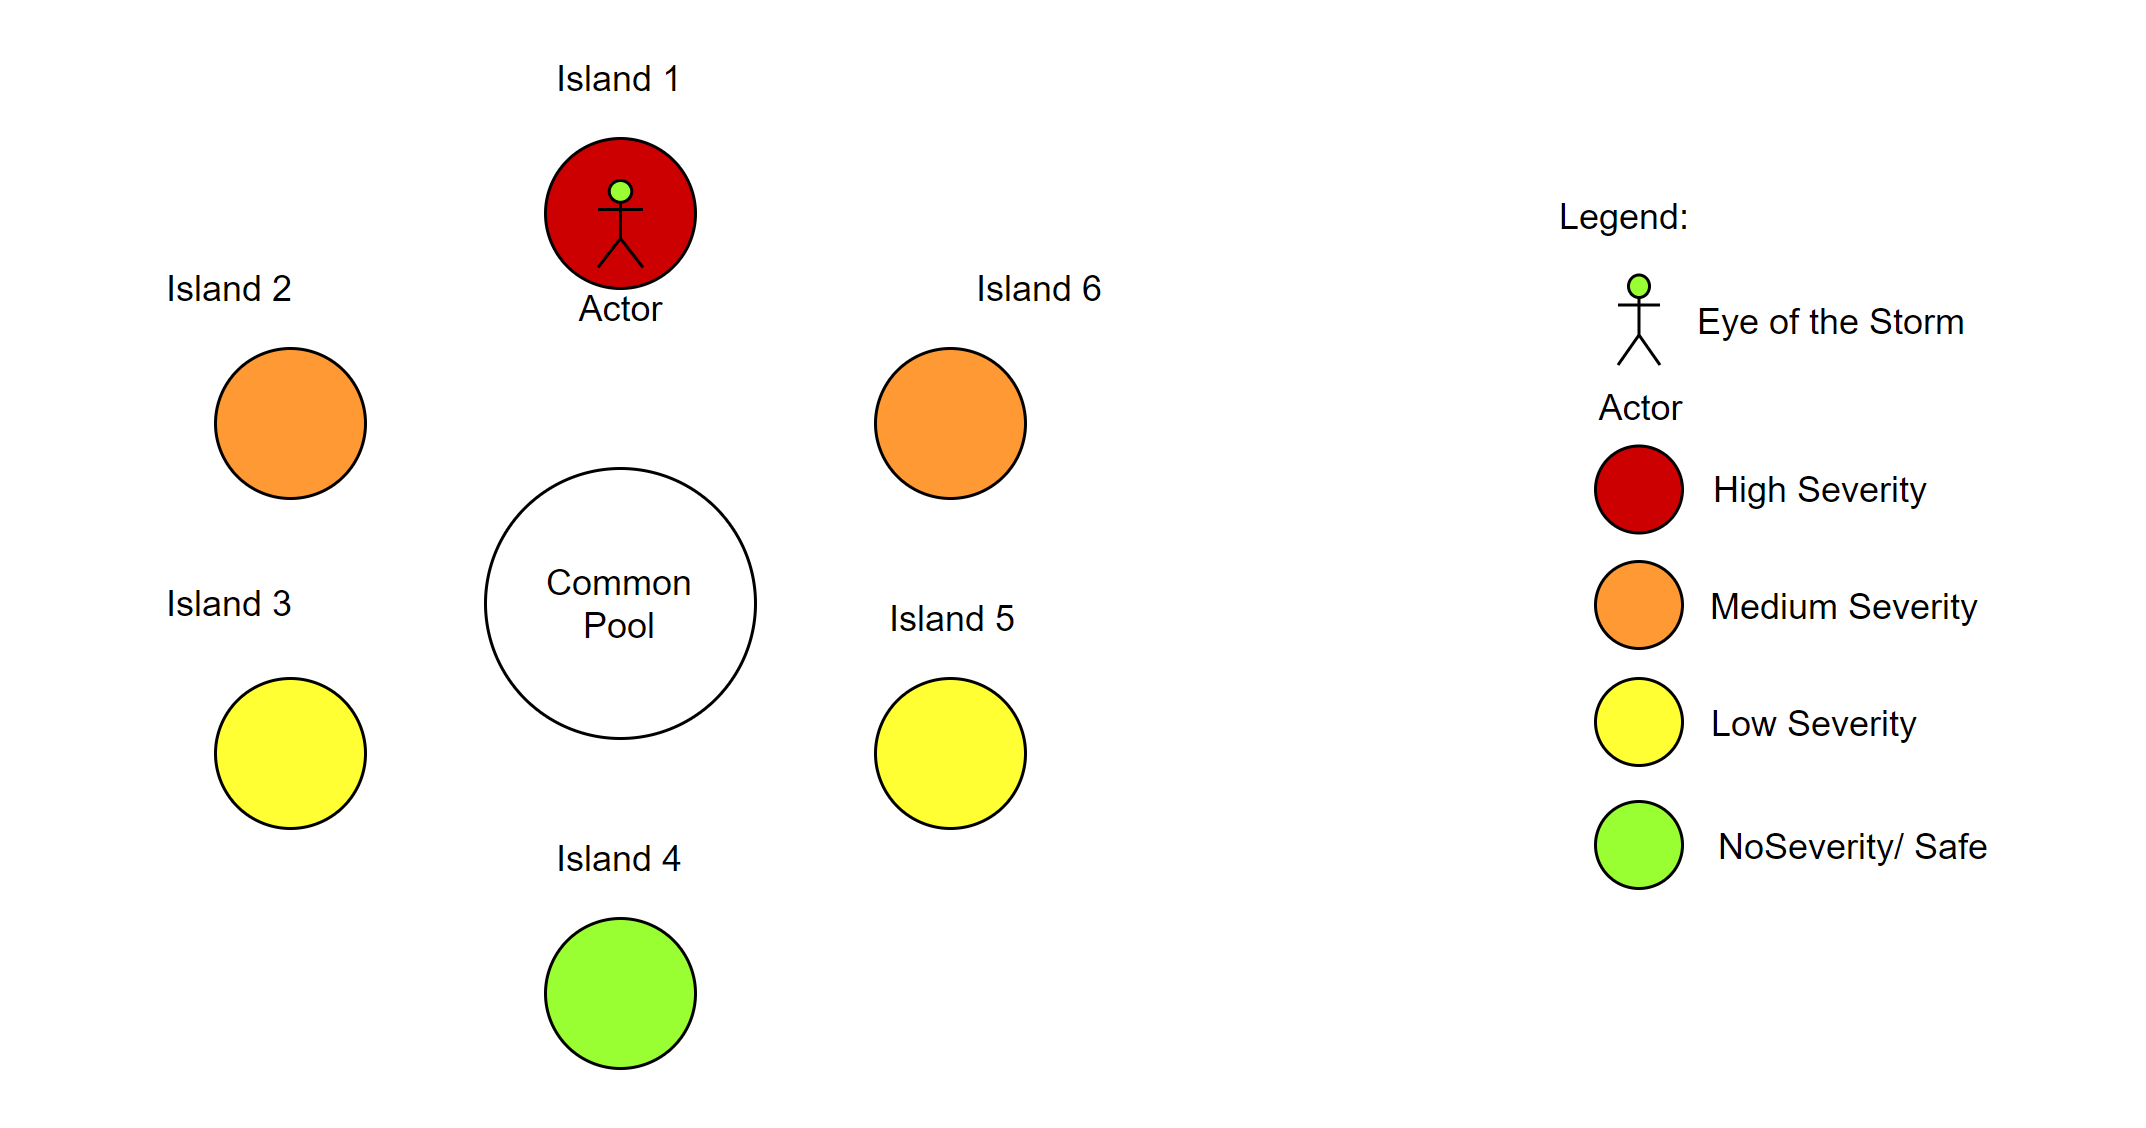
\includegraphics[width=1\textwidth]{04_environment/Images/Disaster eye of the storm severity.PNG}
    \caption{Disaster Epicenter effects}
    \label{Images:Disaster eye of the storm severity}
\end{figure}

\newpage
\subsection{Functions within the Disaster}
It is worth mentioning that the island's geography in infrastructure is the combination of the island number and the island’s fixed location in the archipelago.\\

\begin{table}[h]
\begin{center}
\begin{tabular}{|p{1.1in}|p{1.1in}|p{1.1in}|p{1.1in}|} \hline
\textbf{Functions} & \textbf{Description} & \textbf{Inputs} & \textbf{Outputs} \\ \hline
\textit{Bernouilli Distribution \texttt{(pdfGlobal)}} & Whether a disaster is going to occur & -The probability of a disaster occurring,\newline -The Global probability variable & Determines the likelihood of a disaster occurring \\ \hline
\texttt{PdfMag} & Exponential distribution & -The spatial PDF & Determine the disaster magnitude \\ \hline
\texttt{Epix,EpiY} & Spatial probability distribution function & -The spatial PDF\newline -Disaster Magnitude & Determines the location of the disaster epicentre \\ \hline
\texttt{DisasterEffect} & Island's Proximity distance to the eye of the storm & -Island geography\newline -Eye of the storm location & Determine the islands damage \\ \hline
\end{tabular}
\caption{\label{tab:table-name}Disaster's main functions}
\end{center}
\end{table}

The disaster has been computed as part of the infrastructure: Each island has a fixed position, characterised using Cartesian coordinates. They are located in the archipelago which captures the collection of island geographies including the bounding regions of the entire archipelago.\\

Furthermore, to determine when a disaster is going to occur, we have used the Bernoulli random variable (probability of a disaster occurring is low).\\

The Spatial probability distribution function "Spatial PDF" is uniform and it controls the distribution works of XY grid of the location of the disaster. The magnitude is then exponentially distributed (it exponentially more likely to have a smaller magnitude as we want large disasters to be more rare, occur less frequently). In addition, we have created a magnitude variable "Lambda" which can vary the slope of the exponential function (create a harsher environment when increasing the "lambda variable" by creating larger disasters and vice versa). In addition, the eye of the storm (disaster epicentre) is limited within the bounds of the environment (The environment bounds are fixed, they are specified by the users).\\

\begin{figure}[!htb]
    \centering
    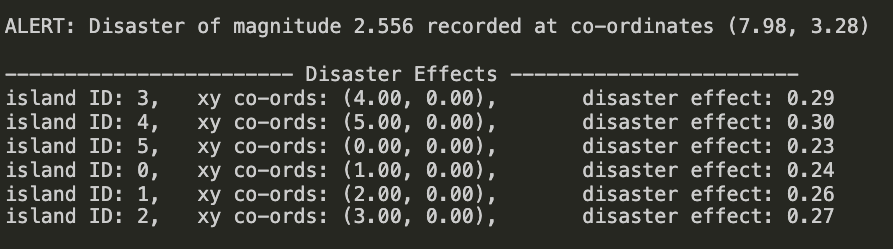
\includegraphics[width=1\textwidth]{04_environment/Images/Disaster output infrastructure.png}
    \caption{Infrastructure Disaster outcome}
    \label{Images:Disaster output infrastructure}
\end{figure}

The image above illustrates the output of the disaster, it first shows the magnitude of the disaster and the precise location of the eye of the storm, it indicates as well the fixed location of each island as well as the proportional effect of each island. For example, Island 2 with a fixed location of (5,0) has the largest disaster effect, which means it is the closest to the eye of the storm.\\

\subsection{Future works Concepts}

The disaster is a random function, meaning that it is possible to predict it with the current game.\\

There are multiple future works ideas that would be developed in the design aspect such as; a deterministic disaster which would be  designed as a straight line that accumulates during the days, once the threshold has been met then the disaster would occur. Another deterministic disaster idea would be to link the disaster’s magnitude to time. Thus, agents will have to learn from past disaster occurrences, creating a memory. Agents will start learning from past disasters and will be able to forecast the next one. Therefore, the agents will be able to forecast that if a disaster did not surface for a long period of time, then the magnitude of the next disaster will be much larger than the previous one.\\

Another Idea is that agents can invest into forecasting. Therefore, agents will have access to a history of past disasters, which would be utilised by the agents to learn and gain knowledge in order to predict the upcoming disaster. The larger the amount of resources invested; the agents will have access to a larger history of previous disasters. Therefore, agents will acquire knowledge, when investing resources.\\

\section{Common Pool}
\subsection{Common Pool Background}

We are designing a game where 6-islands (agents) are having access to a common-pool resource. In micro-level, each island intends to maximise its utility while in macro-level, all the islands want to maintain sustainability and be protected by the upcoming disaster. The above description specifies a collective action problem where n-agents (6 in our case) are seeking access to a common pool resource that is sufficient to satisfy some agents but not to satisfy all of them.\\

We have implemented a Linear Public Goods (LPG) Game where all the agents individually own some resources and try to maintain and increase them, by foraging, but also contribute a part of them to the common pool. This common pool is used for the payment of expenses of the institutional roles and for the protection towards the disaster.\\

In more detail, the common pool is represented by a structure with following characteristics:

\begin{itemize}
    \item Common Pool Threshold
    \item Amount of Resources 
\end{itemize}

According to the specifications of an LPG Game, the agents should be able to perform the following actions:  

\begin{itemize}
    \item Request Resource from the Common Pool 
    \item Contribute Resource to the Common Pool 
\end{itemize}

And the Common Pool is responsible for two more actions: 

\begin{itemize}
    \item Mitigate Disaster
    \item Deplete islands after a disaster
\end{itemize}

\newpage
\subsection{functions within the Common pool}

For each of these action a relevant function has been implemented as follows:\\

\begin{table}[h]
\begin{center}
\begin{tabular}
{|p{1.1in}|p{1.1in}|p{1.1in}|p{1.1in}|} \hline
\textbf{Name} & \textbf{Description} & \textbf{Input} & \textbf{Outcome} \\ \hline
\texttt{islandDistribute} & Distribute Resources from Common Pool to Island upon Request & -Requested Amount of Resources\newline -Island Name & Resources subtracted from CP and added to island \\ \hline
\texttt{islandContribute} & Contribute Resources from Island to Common Pool & -Donated Amount of Resources\newline -Island Name & Resources subtracted from Island and added to CP \\ \hline
\texttt{DisasterMitigate} & Mitigate the Disaster with the Amount of Resources in the Common Pool & - Effect of Disaster to each island\newline - Proportional effect of Disaster to each island (magnitude of disaster divided by the distance of the island from epicenter) & Resources in CP were exploited for the mitigation of the disaster and remaining effect has to be mitigated by each island \\ \hline
\texttt{islandDeplete} & Deplete Islands after the disaster (with the amount of disaster that couldn't be mitigated by CP) & -Remaining effect for each Island\newline -List of Islands & The remaining proportional effect of the disaster to each island is causing the depletion of resources \\ \hline
\end{tabular}
\caption{\label{tab:table-name}Common Pool's main functions}
\end{center}
\end{table}

The common pool has been computed as part of the infrastructure: with a threshold that is the amount of resources to hopefully help to completely mitigate the disaster. If the threshold is met, the damage from the disaster on the common pool and islands will be half the actual amount. This incentivises islands to contribute to the common pool and reflect the reality that, if there is enough preparation for the disaster, the damage will be much less compared to no preparation. Furthermore, it is worth mentioning that the threshold is a fixed value.\\

Another important input to the implementation is the magnitude of the disaster’s damage to each island. As shown in Figure 1.9 , the disaster’s magnitude is 3.458. However, the disaster’s effect on individual islands do not add up to 3.458 because the storm’s epicenter is further away from the islands. This aspect creates a more realistic scenario to the game. From the islands’ individual damage, proportional effects are calculated to determine which island has been hit harder out of the 6 islands. The summation of these proportional effects is equal to 100\%, which is the total effective damage. \\

If the common pool has enough resources to fully mitigate the disaster, the process is very easy. However, in the unfortunate events, the common pool resources will be used to mitigate each island's damage according to their proportional effect i.e., if an island is hit harder, it will receive more help from the common pool. This is also visualized in Figure 1.9, as island 4 withstands most damage from the storm, the common pool gave island 4 most help with 252.47 resources (“common pool mitigated” column). The updated damage value shows the leftover damage of the disaster that the common pool was not able to mitigate. These leftover damage will be used to further deplete the island's private pool of resources. If there are enough resources in the common pool totally mitigate the disaster then the update damage values will be 0.\\

\begin{figure}[!htb]
    \centering
    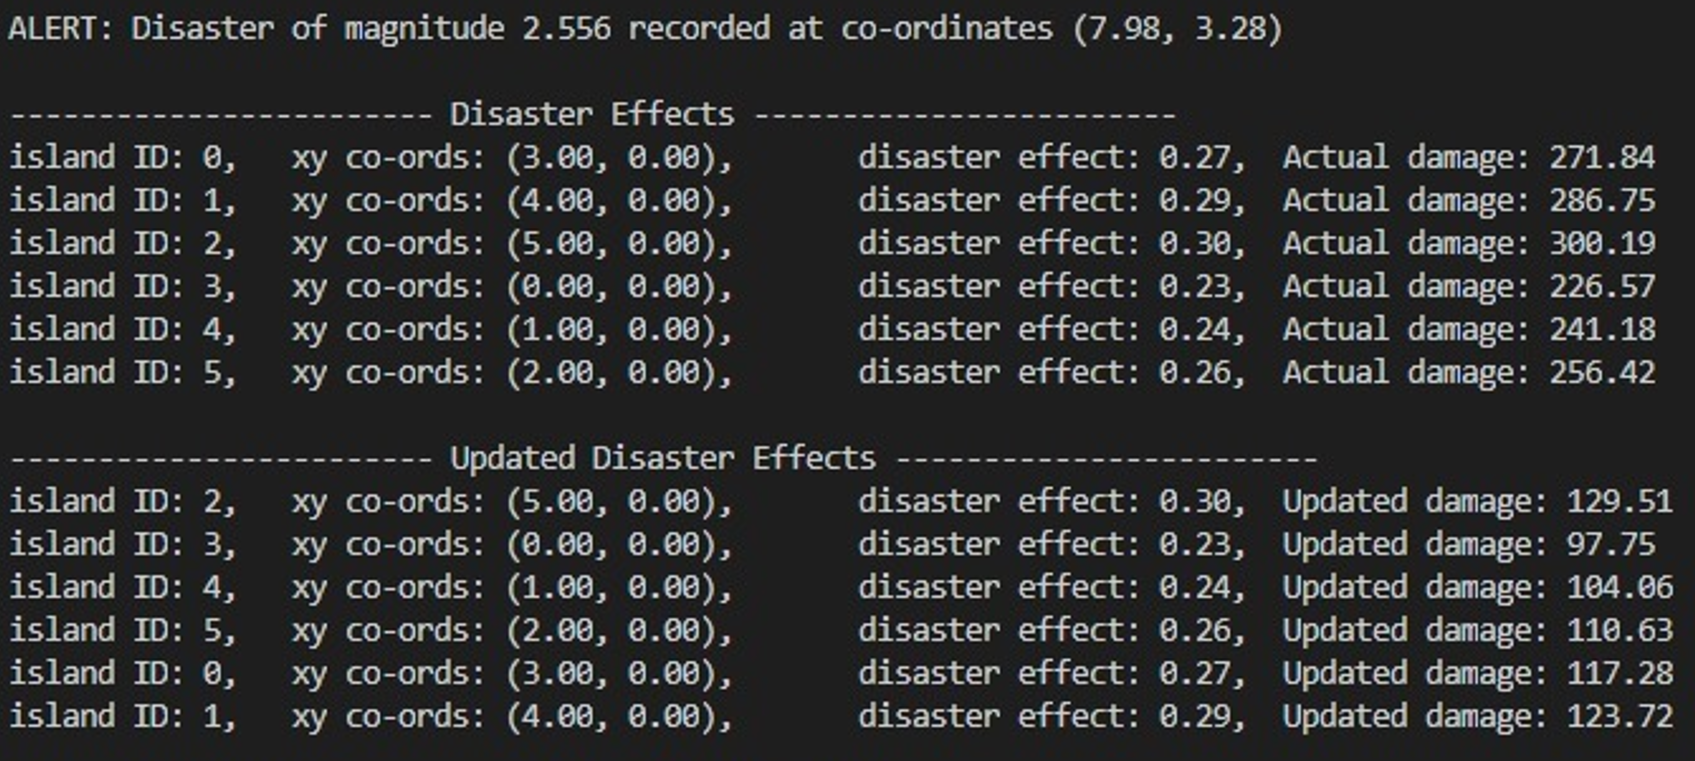
\includegraphics[width=1\textwidth]{04_environment/Images/Common Pool infrastructure outcome.PNG}
    \caption{Demonstration of how common pool works in software}
    \label{Images:Common Pool infrastructure outcome}
\end{figure}

The common pool threshold is a fixed value and known to islands. later, the functionality of making the Threshold unknown to the islands would be added. \\

The common pool resources will be given to each island based on the severity of the damages.\\

If the amount of resources in the common pool exceeds the total effect of disaster, then the leftover amount of resources in the common pool will be used for the next round.\\

Since the goal of each island is to maximise its utility, the following dilemma shows up: islands can free ride by not contributing to the common pool and yet receiving the benefits after a disaster or if they are aware that they would not be depleted by the disaster - since they are far away from the eye of the storm - they might also not contribute to the common pool and thus the rest of the islands would be severely destroyed. \\

The following example can briefly explain this dilemma:\\

If the epicentre of disaster is known to the islands and happens to coincide with the location of Island 1, then Island 4 might not contribute at all to the CP since it will not be affected by the disaster. Moreover, Islands 3 and 5 that will not be severely hit might contribute a small amount to the CP or even zero amount (free riding case). Since the rest of the islands might contribute to the CP, then Islands 3 and 5 will be profited by the contribution of others.\\

We wanted to highlight the importance of prevention and incentivise islands to contribute to the Common Pool, thus if the amount of resources in the common pool exceeds the threshold when the disaster happens, then the “power” of disaster towards the islands and common pool will be decreased. It makes sense in real life, as more preparation will result in less damage. The actual damage of disaster is decreased by half, but this can vary later.\\

\subsection{Example distribution}
This can be described by the examples in table X, which shows 4 possible scenario:\\ 

\begin{itemize}
    \item Contribution to common pool does not meet threshold and common pool cannot fully mitigate disaster’s damage
    \item Contribution to common pool does not meet threshold but common pool can fully mitigate disaster’s damage
    \item Contribution to common pool meets threshold but common pool cannot fully mitigate disaster’s damage
    \item Contribution to common pool meets threshold and common pool can fully mitigate disaster’s damage
\end{itemize}

\begin{table}[h]
\begin{center} 
\begin{tabular}{|p{0.9in}|p{0.9in}|p{0.9in}|p{0.9in}|p{0.9in}|} \hline
& \textbf{Scenario 1} & \textbf{Scenario 2} & \textbf{Scenario 3} & \textbf{Scenario 4} \\ \hline
\textbf{Disaster total damage} & 1000 & 200 & 1200 & 1200 \\ \hline
\textbf{CP's threshold} & 500 & 500 & 500 & 500 \\ \hline
\textbf{CP's current value} & 300 & 300 & 500 & 700 \\ \hline
\textbf{CP's multiplier} & 1 & 1 & 0.5 & 0.5 \\ \hline
\textbf{Mitigated damage} & 300 & 200 & 500 & 1200 \\ \hline
\textbf{Remaining damage} & 700 & 0 & 100 & 0 \\ \hline
\textbf{CP's remaining value} & 0 & 100 & 0 & 100 \\ \hline
\end{tabular}
\caption{\label{tab:table-name}Demonstration of how common works in different scenarios}
\end{center} 
\end{table}

In scenario 1, the disaster total damage is high, however there is no preparation from the islands through contribution to the common pool. As a result, the common pool could not mitigate all of the damage and 70\% of the damage will be directly on the islands\\

In scenario 2, even though there is no preparation, the common pool is still able to mitigate all of the damage thanks to the low damage of disaster. The leftover resource in the common pool will stay there.\\

In scenario 3, the disaster damage is high. Fortunately, the islands have prepared themselves moderately through contribution to the common pool. Thus, the islands only have to take very little leftover damage.\\

In scenario 4, the disaster damage is high and the islands have prepared themselves very well. As a result, the damage is fully mitigated by the common pool and there is still leftover resource in the pool. 


\subsection{Future Works Concepts}
To observe behaviors of agents in different settings, the future works of the common pool will be centered around varying the values of different parameters such as threshold and threshold multiplier. The forecasting function of the disaster part can be used as a tool to variate the common pool’s threshold and multiplier accordingly. In events that damage could be high, the preparation should be done more carefully, thus the common pool’s threshold can be raised to let islands know about potential damage from disaster. The same thing can be done for threshold multiplier, where the multiplier will be greater for bigger disaster. Since threshold and multiplier both encourage the preparation for disaster, one of them can be fixed at certain seasons to observe different behavior of agents when it comes to varying different parameters. 

    \chapter{Inter-Island Governmental Organisation (IIGO)}


The role of IIGO is to maintain, update, and revise the rules concerning provision to managing the long-term collective risk dilemma (ltCRD). 

\begin{itemize}
    \item There will be 3 distinct branches in the IIGO: the \textbf{legislative branch}, \textbf{executive branch} and \textbf{judicial branch}\footnote{This is, as no surprise, inspired by the separation of powers in Western democracies.}.
    \item Each role is put in power according to the  transfer-of-power rules (see Section~\ref{subsec:transfer-of-power} for more detail).
    \item The head of the legislative branch is the Speaker, the head of the executive branch is the President, and the head of judicial branch is the Judge.
    \begin{itemize}
        \item  The Speaker, President and Judge are selected, through a democratic election, from the islands in the archipelago\footnote{This naming is inspired by the roles in the US Government.}.
        \item The resources gathered by the archipelago are endogenous, hence acting on the institutional powers granted to the Speaker, President or Judge costs resources. 
        \item For their duty, the President, the Speaker and the Judge receive a salary for each of their turns in office (see Section~\ref{subsec:salary} for more detail).
        \item The limit of the powers of the President, Speaker and Judge are defined in this chapter (e.g. the Speaker can only call one vote per turn).
 
    \end{itemize}
\end{itemize}

\subsection{IIGO Specific Definitions}
\begin{definition} \label{def:ballot}
    A \textbf{ballot} is related to each island's \textbf{power} to support or disagree with the rule specified in the vote called by the President and to vote in favour or against an island for a specific role (i.e. the President, Speaker, Judge) at each round of the game.
\end{definition}


%\begin{definition} \label{def:vote}
    %A \textbf{vote} is related to a role's (i.e. the President, Speaker, Judge) \textbf{power} to call a vote for a specific rule or an election.
%\end{definition}


\begin{definition} \label{def:tax}
    The \textbf{taxation} is related to the President's \textbf{power} to request a specific \underline{\textbf{minimum}} amount of contribution from each island to the common pool at each round of the game. 
\end{definition}

\begin{definition} \label{def:alloc_req}
    An \textbf{allocation request} is related to each island's \textbf{power} to request a specific amount of resource allocation from the President at each round of the game.
\end{definition}


\begin{definition} \label{def:rule_prop_list}
A \textbf{rule proposal list} is related to each island's \textbf{power} to propose a specific rule to be passed to the President at each round of the game.
\end{definition}

\begin{definition} \label{def:invst}
    An \textbf{investigation} is related to the Judge's \textbf{power} to acquire information to make a decision, followed by a calculation of the expected results and checking whether some specific rules have been obeyed, exclusively for the actions carried out by the \textbf{islands}. 
\end{definition}


An example of an \emph{investigation}: The President has permitted the island $X$ to take the amount of $Y$ resources from the common pool. Upon \emph{investigation} carried out by the Judge, it is revealed that the amount of resources taken out from the common pool by the island $X$ is, in fact, $Y'$ such that $Y' \neq Y$.


\begin{definition}
\textbf{Monitoring} is a government official's \textbf{power} to perform event recognition and to check whether some specific rules have been obeyed.
\end{definition}

An example of \emph{monitoring}: The Speaker has performed only the following action: \emph{counted the votes and calculated the result} for a rule. Upon \emph{monitoring} carried out by the President, it is noticed that the Speaker has not made any \emph{announcement}. Hence, the Speaker has not followed their obligation to \emph{announce} the result of any vote held.

See Section~\ref{sec:accountability} for more information about which roles can monitor which ones.


\begin{definition}
\textbf{Investigative-monitoring} is a government official's \textbf{power} to acquire the information used in acting on a governmental power followed by calculation of the expected results and checking whether some specific rules have been obeyed, exclusively for the actions carried out by a government official they are responsible for.
\end{definition}

An example of \emph{investigative-monitoring}: The Speaker has performed the following actions: \emph{counted the votes and calculated the result $R$} for a vote $V$ and \emph{announced} the result $R'$ for the vote $V$. Upon \emph{investigative-monitoring} carried out by the President, it is noticed that $R' \neq R$. Hence, the Speaker has modified the announced result.


\begin{definition}
The \textbf{sanction} is related to the Judge's \emph{power} to punish non-compliant islands when their disobedience is confirmed through investigations at a specific turn.
\end{definition}


\begin{definition}
The (judicial) \textbf{pardon} is related to the Judge's \emph{power} to forgive a non-compliant island at a specific turn.
\end{definition}

\begin{definition}
The \textbf{budget} is the maximum amount of resources a role is permitted to spend from the common pool as it performs its own institutional-power-enabled actions at a specific turn.
\end{definition}


\begin{definition}
The \textbf{salary} is the amount of resources a role is to be given from the common pool as a reward for performing its institutional-power-enabled actions at a specific turn.
\end{definition}

\begin{definition} \label{def:term}
A \textbf{term} is the number of turns an island is \emph{permitted} to hold a role, and after which the responsible role (indicated in the transfer-of-power cycle in Figure~\ref{fig:cycles_in_IIGO}) is \emph{obliged} to initiate transfer-of-power.
\end{definition}

\subsection{\emph{Power}, \emph{Permission} and \emph{Obligation} Distinction}
In the rest of the specifications, we will be specifically using the following three terms to define the actions and responsibilities carried out by the Speaker, President, Judge (see Figure~ \ref{fig:per_obl_sets}):
\begin{itemize}
    \item Power
    \item Permission
    \item Obligation
\end{itemize}



\begin{figure}[H] 
\centering
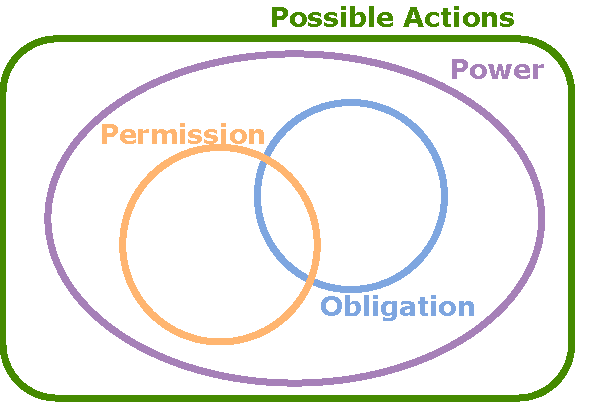
\includegraphics[width=0.6\textwidth]{05_iigo/images/SOMAS_per_obl.pdf}
\caption{Relationship between \emph{power}, \emph{permission} and \emph{obligation}.}
\label{fig:per_obl_sets}
\end{figure} 


For example, the Judge has the \emph{power} to carry out investigations at an IIGO session. There are no rules specifying which specific islands the Judge should investigate. Therefore, the Judge has the \emph{permission} to investigate any `alive' islands during a session. However, the Judge is \emph{obliged} to make at least some number of investigations each turn.



\section{Executive Branch}
\label{sec:executive}
The executive branch is responsible for \textbf{carrying out the law}.
\begin{itemize}
       
    \item The President has the \emph{power} to: 
    \begin{itemize}
        
        \item Select a rule for voting $R^{*}$ to be passed to the Speaker.
        \begin{rule_IIGO}
            The President has the \emph{obligation} to \emph{select} a rule $R^{*}$ if the \emph{rule proposal list} has at least one proposed rule in it.
        \end{rule_IIGO}
        \begin{rule_IIGO}
            The President has the \emph{permission} to \emph{select} a rule $R^{*}$ if and only if $R^{*} \in S$, where $S$ is the \emph{rule proposal list}.
        \end{rule_IIGO}
        
        \item Decide the amount of individual \emph{taxation} (i.e. a specific \emph{minimum} amount of contribution to the common pool for each island) for the current turn.
        
        \begin{itemize}
            \item The President is given the self-reported resource amounts held by each island to assist in this decision.
            %\item Suggested Rule: For any island that has chosen to not report it's resources, the President has the \emph{obligation} to set them an individual tax amount T.
        \end{itemize}
        
        \item Decide the allocation of resources distributed from the common pool to the islands (i.e. a specific \emph{maximum} amount an island is permitted to take from the common pool).
        
        \begin{itemize}
            \item The President is given the \emph{allocation requests} made by each island.
            %\item \emph{}{Suggested Rule:} The President has an obligation to prioritise islands in critical condition.
        \end{itemize}
    \end{itemize}
\end{itemize}



\section{Legislative Branch}
\label{sec:legislative}
The legislative branch is responsible for \textbf{making the law}.
\begin{itemize}

    \item The Speaker has the \emph{power} to:
    \begin{itemize}
        
        \item Call a vote $V$ for a rule $R$.
        \begin{rule_IIGO}
            The Speaker has the \emph{obligation} to \emph{call} a vote $V$ if and only if the President has \emph{selected} a rule $R$ to be voted on.
        \end {rule_IIGO}
        \begin{rule_IIGO}
            The Speaker has the \emph{permission} to \emph{call} a vote $V$ for a rule $R$ if and only if the rule $R = R^{*}$, where $R^{*}$ is the rule \emph{selected} by the President.
        \end {rule_IIGO}
            
        \item Choose which islands are participating in the vote $V$.
       % \footnote{This is our sequential implementation alternative for the power to close the ballot box.}.
        \begin{rule_IIGO}
            The Speaker has the \emph{obligation} to ask for a vote from all alive islands.
        \end {rule_IIGO}
            
        \item Declare the result $C$ of a vote $V$. 
        \begin{rule_IIGO}
            The Speaker has the \emph{obligation} to \emph{declare the result} $C$ for a vote $V$ if and only if the vote V has been \emph{called}.
        \end {rule_IIGO}
        \begin{rule_IIGO}
            The Speaker has the \emph{permission} to \emph{declare the result} $C$ for a vote $V$ if $C = C^{*}$, where $C^{*}$ is the result produced by \emph{calling} the vote $V$.
        \end {rule_IIGO}
        \begin{itemize}
            \item This step is what enables a rule to be \emph{active}.
        \end{itemize}
    \end{itemize}
\end{itemize}




\section{Judicial Branch}
\label{sec:judicial}

The judicial branch is responsible for \textbf{evaluating the law}.
\begin{itemize}
    \item The Judge has the \emph{power} to:
    \begin{itemize}
        \item Perform a number of \emph{inspections}\footnote{An \emph{inspection} \textbf{costs} an expense of resources (See Definition~\ref{def:invst} for more detail).} $I$ and produce a compliance outcome $\mathbb{O}^{*}$\footnote{Note that the compliance outcome $\mathbb{O}^{*}$ considered is a boolean.}.
        %(true: the island has been compliant with the rules in play, false: the island has not been compliant with the rules in play)
        %\begin{itemize}
           % \item For example, to check if the event outcome is \emph{concurrent}\footnote{Again, what is defined as "concurrent"? A clear definition is needed.} with the rules.
        %\end{itemize}
        \begin{rule_IIGO}
            The Judge has the \emph{obligation} to make at least $N$ investigations at each turn.
        \end{rule_IIGO}
        \item Declare the outcome $\mathbb{O}$ of an inspection $I$ to all islands\footnote{This act of broadcasting is especially important for islands to form an opinion about the sanctioned islands accordingly.}.
        \begin{rule_IIGO}
            The Judge has the \emph{obligation} to declare the outcome $\mathbb{O}$ of an inspection $I$ if and only if the inspection $I$ has been performed.
        \end{rule_IIGO}
        \begin{rule_IIGO}
            The Judge has the \emph{permission} to declare the outcome $\mathbb{O}$ of an inspection $I$ if $\mathbb{O} = \mathbb{O}^{*}$, where $\mathbb{O}^{*}$ is the outcome of the inspection $I$.
        \end{rule_IIGO}
        %\item Initiate the removal of the \texttt{President}.
        %\begin{itemize}
            %\item A good Judge would be especially vigilant during \emph{power transfer} regarding the \emph{President} position (see Section~\ref{leg_const} for more detail).
        %\end{itemize}
        \item Invoke economic \textbf{sanctions} (see Section~\ref{sec:sanctions} for more detail).
        \begin{rule_IIGO}
            The Judge has the \emph{obligation} to invoke a sanction $S$ for an island $X$ if and only if an investigation $I$ has an outcome $\mathbb{O}^{*}$ indicating non-compliance, and $I$ is an investigation of an action taken by island $X$.
        \end{rule_IIGO}
        \item Invoke even more severe sanctions in the case of further disobedience to previous sanction(s).
        \begin{rule_IIGO}
            The Judge has the \emph{permission} to invoke a severer sanction $S'$ for an island $X$ if the island $X$ has not fulfilled the requirements of the previous sanction $S$.
        \end{rule_IIGO}
        \item Pardon the islands which are currently sanctioned.
        \begin{rule_IIGO}
            The Judge has the \emph{permission} to revoke any sanction $S$ of an island $X$ at a specific turn.
        \end{rule_IIGO}
    \end{itemize}
\end{itemize}
%(e.g. a new rule that falls under a "sanction" category \hl{[I'm not sure about this being a `new rule` [Ezgi]]}

\subsection{Sanctions}
\label{sec:sanctions}
All sanctions are of economic nature which include:
        \begin{itemize}
            %\item Revoking an island's access to the common pool.
            \item Enforcing an island to contribute a specific amount of resources to the common pool.
            \begin{itemize}
                \item This does not mean that the Judge has the \emph{power} to take resources from an island in order to put them to the common pool -- the island itself is expected to carry out this implication imposed by the sanction itself, otherwise further punishment can be induced by the Judge.
                \item Similarly, \emph{opinion formulation} will follow accordingly whether the island(s) is/are following the implications imposed by the sanction(s).
            \end{itemize}
        
    \end{itemize}
    Sanctions are the associated penalty that comes with an island breaking a specific rule. The Judge is in full control of the penalties associated with breaking any rules. Once the Judge has specified the score of the penalty associated with each time an island breaks a rule, the cumulative penalties accumulated by the island are then used to determine which \textbf{sanction tier} that each island falls into. The score threshold to determine the boundaries of the sanction tiers are set by the Judge. At each turn of the game, each island is told whether they are being sanctioned, and if so, which \textbf{sanction tier} that they are currently in. The \textbf{sanction tiers} of the non-compliant islands are also broadcasted to the other islands in the archipelago. To summarise, the sanctioning process follows these steps:
    
    
    
    %Sanctions are based on an island breaking a rule. Each rule must therefore have an associated penalty. By default, we set these penalties such that they add $1$ to the total sanction score for each island. However, we allow the judge to override this scoring, the judge is able to set their own scores for any particular rule as they desire. This custom scoring is then used when an island breaks a particular rule. By looking at events that occurred in the last turn, and using the customised scoring we provide the holder of the judge role with full control of the penalties for breaking any rules.
    
    





%we then use the cumulative penalties accumulated by each island to determine which Sanction Tier they fall into. The score threshold's required to fall into these sanction tiers is set by the judge and is checked for monotonicity. Each island is told whether they are being sanctioned, and is so what tier they are in. We also tell other islands about which sanction tiers other islands have fallen into. 

    \begin{enumerate}
        \item The Judge has the \emph{power} to set custom penalties associated with breaking any rules.
        \item The Judge is given a list of all events that occurred in the previous turn.
        \item The Judge has the \emph{power} to check whether any, or all of these previous events, involve the islands in the archipelago breaking any rules.
        \item Each of the transgressions is scored using the Judge's custom penalties if the Judge has set them. Otherwise, a score of $1$ is given each time a rule is broken.
        \item The Judge has the \emph{power} to revise the sanction thresholds.
        \item Using the latest sanction thresholds available, each island is assigned to a sanction tier based on the sanction score that it has received.
        \item These sanction tiers are broadcasted to all of the islands in the archipelago.
        \item The Judge then uses sanctions rules in place to calculate the specific amount of resources that each non-compliant island has in order to determine how much it should contribute to the common pool, based on the sanction tier that it is in.
    \end{enumerate}



\section{Constitutional Rights and Obligations in the Archipelago}
\label{sec:const_rights_obl_archi}
Each island has the \emph{power} to:
\begin{itemize}
\item make an \emph{allocation request} (see Definition~\ref{def:alloc_req}) to the President for a specific amount to be allocated to them.
\item report the number of resources it is in possession of to the President.
\begin{rule_IIGO}
    Each island has the \emph{obligation} to report the number of resources it is in possession of to the President.
\end{rule_IIGO}
\begin{rule_IIGO}
    Each island has the \emph{permission} to report the number of resources $R'$ if and only if $R' = R$, where R is the number of resources the island is in possession of.
\end{rule_IIGO}
\item take resources from the common pool.


\begin{rule_IIGO}
    Each island has the \emph{permission} to take at maximum $N$ resources, where $N$ is the specific allocation made by the President to that island\footnote{If no such allocation is made, the island is \emph{permitted} to take any amount of resources.}.
\end{rule_IIGO}
\item contribute resources to the common pool.
\begin{rule_IIGO}
    Each island has the \emph{obligation} to contribute to the common pool an amount greater or equal to that of the individual tax set by the President.
\end{rule_IIGO}
                %The President is in
                %(unless there is a rule in place that dictates how Speaker is to allocate resources).
\item add a rule to the \emph{rule proposal list} (see Definition~\ref{def:rule_prop_list}) at the start of each turn.
        %\begin{itemize}
            %\item The game specification includes how many rules an island can propose each turn.
        %\end{itemize}
        %\item vote  for rules in the Legislative Branch and vote for their favourite islands in elections
\item participate in the legislative branch of the government by casting ballots in votes called by the Speaker
\item vote for an island to be elected for a specific role (e.g. the President, Judge, Speaker) during the elections\footnote{This will be assumed to be true \underline{unless stated otherwise}. %Note that \textbf{diplomatic sanctions} can disable this power of a specific island (see Section~\ref{jud_const}).}.
        }.
\end{itemize}
\section{Accountability Cycle}
\label{sec:accountability}


To ensure that the government avoids corruption and abuse of power, each branch is accountable to another. The President is accountable to the Speaker, the Speaker is accountable to the Judge, and the Judge is accountable to the President (see Figure~ \ref{fig:cycles_in_IIGO}). This accountability cycle is enacted through \emph{monitoring} actions\footnote{Note that the terms \textbf{monitoring} and \textbf{investigation} have similar but quite different meanings in the IIGO context.}. 

The powers related to the accountability cycle and transfer-of-power for each role can be summarized as the following: 
\begin{itemize}
    \item The Speaker has the \emph{power} to: 
    \begin{itemize}
        \item monitor the President.
        \item announce the result of this monitoring.
        \item initiate the transfer-of-power for the Judge.
    \end{itemize}
    \item The President has the \emph{power} to: 
    \begin{itemize}
        \item monitor the Judge.
        \item announce the result of this monitoring.
        \item initiate the transfer-of-power for the Speaker.
    \end{itemize}
    \item The Judge has the \emph{power} to: 
    \begin{itemize}
        \item  monitor the Speaker.
        \item announce the result of this monitoring.
        \item initiate the transfer-of-power for the President.
    \end{itemize}
\end{itemize}

%Unlike investigations performed by the Judge, who performs investigations on island actions in the following turn, each role is given the opportunity to check up on the actions of the role it is responsible for immediately after they have been performed. In this sense, the President can monitor (includes investigative-monitoring) the powers (calling a vote and announcing the result) acted on by the Speaker immediately after the Speaker's announcement (or lack there of). The government officials hold a lot of power so this is to ensure that any wrong-doing is determined as quickly as possible. For this project we are only pursuing one degree of monitoring, that is, the powers relating to the accountability cycle will not be monitored themselves. We assume that agents will act in the interest of themselves and keeping all the islands alive is beneficial to everyone. Hence, while the agents might be inclined to break rules in order to benefit themselves, anyone else breaking the rules is seen as undesirable under the assumption that the system in place is there to benefit all. 


Through the proposed accountability cycle, each role is given the opportunity to check up on the actions of the role it is accountable for immediately after they have been performed. It is clear that the IIGO roles (i.e. the President, Speaker and Judge) hold a considerable amount of \emph{power} in their hands. The accountability cycle is designed to address the possible abuses of this power. With monitoring, any wrong-doing in the IGO is determined as quickly as possible and the role in question can be replaced. 

Within the scope of the coursework, we decided to pursue only \emph{one degree of monitoring}, meaning that the powers relating to the accountability cycle will not be monitored themselves. We assume that agents will act in the interest of all the islands in the archipelago. Hence, while the agents might be inclined to break the rules to benefit in some form, it is assumed that the others will negatively see any non-compliant islands based on the assumption that the proposed IIGO system is in place to maintain the welfare of all the islands.

Let role $X$ be accountable to the role $Y$, which is accountable to the role $Z$. Then:
\begin{rule_IIGO}
$Y$ has the \emph{obligation} to declare the outcome of the monitoring result $M$ associated with the action $A$ undertaken by $X$ if and only if $Y$ has monitored the action $A$ performed by $X$. 
\end{rule_IIGO}
\begin{rule_IIGO}
$Y$ has the \emph{permission} to declare the monitoring result $M$ associated with the action $A$ undertaken by $X$ if and only if $M = M^{*}$, where $M^{*}$ is the outcome of \emph{monitoring} action $A$ performed by $X$\footnote{These constitutional rules should be available to the agents to check their decision against. However, due to having only one degree of accountability cycle in place, these rules are not enforced through any sanctions (i.e. breaking these rules has no consequences as they only deem to be an \emph{agreement} among the roles).}.
\end{rule_IIGO}


\begin{figure}[!htb]
\centering
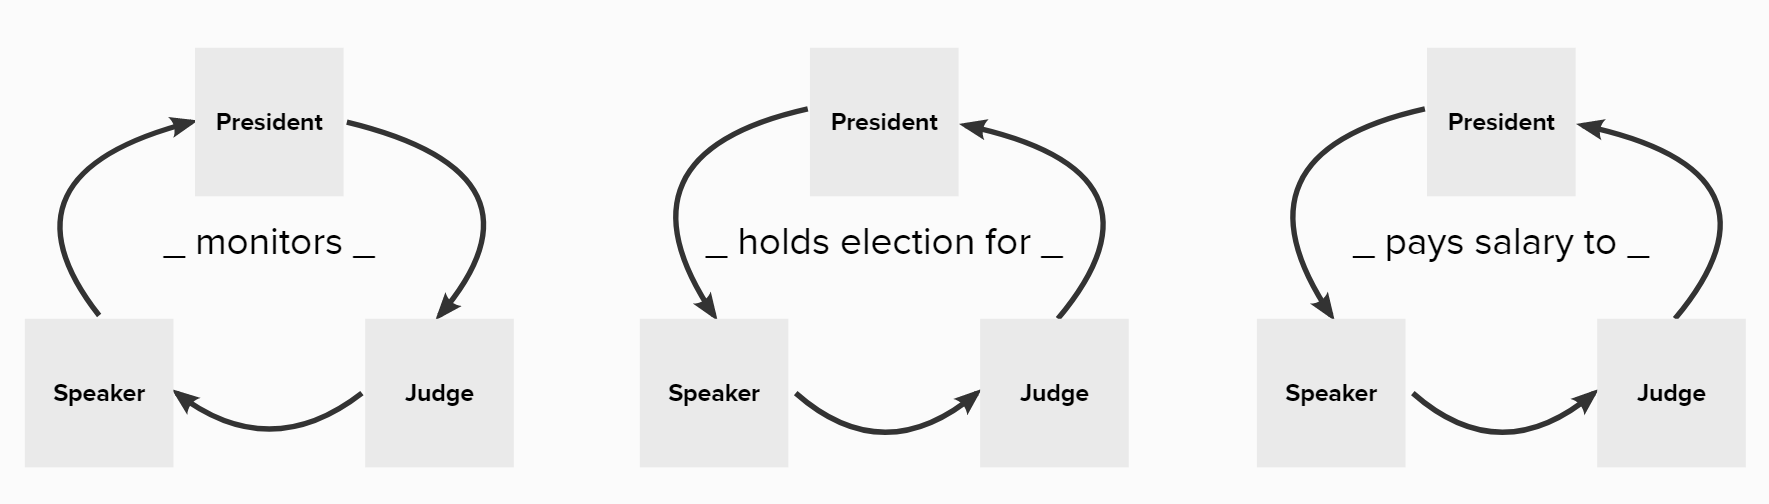
\includegraphics[scale=0.33]{05_iigo/images/role cycles.png}
\caption{Accountability cycle (left), the transfer-of-power cycle (middle) and salary cycle (right).}
\label{fig:cycles_in_IIGO}
\end{figure}


\subsection{Transfer-of-power}
\label{subsec:transfer-of-power}
\begin{enumerate}
    \item The Speaker conducts a vote for the election of the new Judge.
    \item The Judge conducts a vote for the election of the new President.
    \item The President conducts a vote for the election of the new Speaker.
\end{enumerate}
Refer to the Figure~ \ref{fig:cycles_in_IIGO} for further clarification about the transfer-of-power cycle.

\begin{rule_IIGO}
   The role $X$ has the \emph{obligation} to conduct a vote for the election of $Y$ at the end of the term (see Definition~\ref{def:term}) if and only if the role $X$ is accountable to the role $Y$. 
\end{rule_IIGO}.

\section{Budget and Salary}
\subsection{Budget}
%Actions associated with the IIGO have an associated cost that is defined as a configuration parameter. The institutional-power-enabled actions of  identified to require a "computational" component are:

Institutional-enabled-power actions in the IIGO have an associated cost with them. Some examples for such actions include:


%that is defined as a configuration parameter. The institutional-power-enabled actions of  identified to require a "computational" component are:


%We have defined the resource to be an endogenous one, hence any computation surrounding the distribution of the resource must use up some of that resource. 
\begin{itemize}
\item Calling any vote and computing the winner.
\item Declaring (e.g. \textit{announcing} the result of a vote).
\item Setting the amount of \emph{taxation} for each island.
\item Deciding the allocation distribution for each island.
\item Inspecting an island's action history.
\item Monitoring a role.
\end{itemize}

Since IIGO has been designed to act in the common good, IIGO-related costs will be directly withdrawn from the common pool. Since the common pool is considered a communal property of the archipelago, there are rules in place to limit how much each role is allowed to spend in order to perform its own institutional-power-enabled actions. This is the reason why defining the \emph{budget} and keeping it separate for each of the three IIGO roles.


As a role performs institutional-enabled-power actions, the corresponding cost associated with this action is subtracted from the role's budget. A budget of zero means that the role does not have the \emph{power} to perform any of its institutional-power-enabled actions. The removal of the budget rule from the rules in play means the role is allowed to perform as many such actions as it prefers to (as long as those actions are not governed by other rules). 



%As a role performs an endogenous-cost action, the corresponding cost associated with this action is subtracted from the role's budget. Thus, if as a result of an endogenous-cost action a role will be left with negative budget, it will have gone over the budget limit and will have broken the budget rule. A budget of zero means that the role is not allowed to perform any of its institutional-power-enabled actions associated an endogenous-cost. The removal of the budget rule from the rules in play means the role is allowed to perform as many such actions as it pleases (as long as those actions are not governed by other rules). 

The budget rule is also persistent across turns. This means that, assuming nothing else affects the budget, if a role has $100$ resources in its budget at each turn and spends only $10$ resources, this means that this very same role has $90$ resources in its budget at the next turn. On the other hand, islands can choose to increase the budget periodically every turn. This is governed by another budget extension rule.




%one turn and it spends 10, it has 90 resources in it's budget the next turn. 

Finally, it must be noted that the budget is inherently linked with the fact that whether obligations of a specific role can be undergone.
For example, during \emph{monitoring}, it should not be seen as a rule violation if a role has not acted on an obligation if it would go over the budget as a result. 

%This can also be seen as an added clause "... and the action is only permitted if they have the budget" to most rules which govern actions with an endogenous-cost.
%\begin{rule_IIGO}
    %The budget is increased by an amount $N$ every turn.
%\end{rule_IIGO}

%This rule means that, assuming nothing else affects the budget, if a budget is set to increase by 10 resources every turn and the budget is a 100 resources in turn one, the budget is 110 resources in turn 2. Setting this rule to 0 is equal to removing this rule and it means that the budget is never increased. 


\subsection{Salary}
\label{subsec:salary}
A salary is paid to each role in power as an incentive to act in a publicly approved way. %Hence, each role has the \emph{power} to pay a salary to another role following the salary cycle in Figure~\ref{fig:cycles_in_IIGO}.
\begin{rule_IIGO} \label{rule:salary}
   %Each role has the \emph{obligation} to pay the salary of amount $S$ to another if and only if the amount paid $S'$ is equal to $S$.
   Each role has the \emph{obligation} to pay the salary of amount $S$ to one another following the salary cycle in Figure~\ref{fig:cycles_in_IIGO}.
\end{rule_IIGO}

In Rule~\ref{rule:salary}, setting $S=0$ (through changing the active rules in place) means that roles do not have the permission to pay any salary. Removing the Rule~\ref{rule:salary} means that the roles may freely choose the amount $S$ for the salary payments.

\section{IIGO Session order}

\begin{enumerate}
    \item The Judge has the \emph{power} to check the history of actions to confirm whether the previously punished island(s) has/have obeyed the previous round's sanctions, meaning whether they contributed to the common pool accordingly in case of economic sanctions.
    %\begin{itemize}
      %  \item \emph{Suggested Rule:} In case of disobeying sanctions, the Judge is \emph{obliged} and \emph{permitted} to increase the severity of sanctions with respect to specific islands.
   % \end{itemize}
    \item The Judge has the \emph{power} to carry out \emph{inspections} on the history of actions of any island $X$ to check whether:
        \begin{enumerate}
        \item the reported resources of $X$ in the previous round match the real value of resources $X$ had in its private pool for the previous turn.
        \item the island $X$ has retrieved the right amount of the resources from the common pool, based on the \emph{allocation request} evaluated by the previous President.
            \begin{itemize}
            \item An example: In the previous round, the President has decided that the island $X$ can take $Y$ amount of resources from the common pool. If the Judge finds out that the island $X$ has taken an amount of $Y'$ such that $Y' > Y$, the Judge has the \emph{power} to invoke sanctions on the island $X$.
            
            %the Judge is \emph{obliged} and \emph{permitted} to sanction island $X$.
            \end{itemize}
        \end{enumerate}
    \item The Judge has the \emph{power} to invoke sanctions based on the outcome of the inspections.
    \item The President has the \emph{power} to decide to carry out a \emph{monitoring} on:
        \begin{enumerate}
        \item the sanctions imposed by the Judge.
        \end{enumerate}
    \item The islands may report the resources in their private pools to the President.
    \item The President has the \emph{power} to let each island know about the amount of \emph{taxation} they have to pay.
    \item The island has the \emph{power} to make an \emph{allocation request} to the President.
    \item The President has the \emph{power} decide on an allocation of resources and let each island know about the amount of resource allocation they are permitted to take from the common pool.
    \item The island has the \emph{power} to pick and to propose a rule to be voted on to the President.
    \item The President has the \emph{power} to choose a rule to be voted on from the received rule proposals.
    \item The Speaker has the \emph{power} to decide to carry out a \emph{monitoring} on: 
        \begin{enumerate}
        \item the resource allocation decided by the President.
        \item the rule proposed by the President.
        \end{enumerate}
    \item The Speaker has the \emph{power} to call a vote.
        \begin{enumerate}
        \item The islands vote in support of, or against, the rule (aye or nay) anonymously.
        \end{enumerate}
    \item The Speaker has the \emph{power} to announce a result of a vote to the islands and carries out the law change, if required (e.g. deleting/rejecting a rule if there is a majority nay vote).
    \item The Judge has the \emph{power} to decide to carry out \emph{monitoring} on:
        \begin{enumerate}
        \item the vote called by the Speaker.
        \item the Speaker announcing the result.
    \end{enumerate}
    \item The roles pay salary for one another following the accountability cycle in Figure~ \ref{fig:cycles_in_IIGO}.

\end{enumerate}



\section{Future Work}

\begin{itemize}
    \item \textbf{Diplomatic sanctions}: Although having the potential of being a good alternative for severer sanctions discussed in  Section~\ref{sec:sanctions}, diplomatic sanctions are \emph{not} implemented within the scope of the coursework. \\
    Suggested diplomatic sanctions include:
        \begin{itemize}
            \item Revoking an island's eligibility to vote and to be elected for a position.
            \item Revoking an island's eligibility to propose a rule/motion.
        \end{itemize}
    \item \textbf{Immutable rules}: Within the scope of the coursework, a subset of rules could have been categorised as immutable. This means that to change such immutable rules, the islands first need to vote to change their status to be \emph{mutable}, and consequently, hold another vote to change these mutable rules.
    %\item \textbf{Adding rules to the proposal list: } 
\end{itemize}

    \chapter{Inter-Island Trade Organisation (IITO)}

\section{Design}
\label{sec:IITO:Design}

The role of IITO is to facilitate inter-island communication and to enable the acts of giving and receiving gifts. In a more complete and realistic multi-agent simulation, unrestricted communication between the islands could have been considered, where islands could communicate with one another in an unconstrained manner. However, such a communication style would also assume the fact that the islands are rather complex agents which are able to undertake considerably sophisticated actions. Therefore, for the coursework, specific forms of communication were chosen to sensibly restrict the island complexity while still allowing for interesting interactions between the islands to take place.

\subsection{Inter-Island Communication}  
\label{subsec:IITO:inter_island_communication}

Islands which can communicate separately from the main governing body level of interactions (i.e. IIGO) makes more complex island behaviour possible. With the implemented systems, islands can:

\begin{itemize}
    \item Form a group with other islands for collective foraging.
    \item Decide where their foraging group will forage.
    \item Inform other islands of the amount they intend to to donate to the common pool.
    \item Share voting history with other islands.
    \item Share tax amount history with other islands.
    \item Inform other islands of the amount of resources they currently have in their private pool.
\end{itemize}

\textbf{Team Foraging}: Allows islands to decide between each other whether they will forage together and where they will forage. In this way, islands can cooperate with the others that they trust while avoiding other islands that they deem to have misbehaved or broken rules in the past. If islands suspect that some specific islands have deliberately freeloaded in the previous forages, they may also want to avoid foraging with such islands that have contributed less than what they were supposed to.

\textbf{Common Pool Donations}: Allows islands to broadcast how much they plan to donate to the common pool and let them declare to the other islands if they plan to donate more than the specified tax amount put forward by the President as a form of virtue signalling. This may help an island redeem itself if it had previously lost trust. Note that an island can lie about the amount it will donate to the common pool if it is trying to maliciously gain favour.

\textbf{Voting History}: Islands can request voting history from other islands or provide their own one unprompted. This interaction enables islands to verify whether the Speaker has been honest when counting the votes for a previously held election. Note that the islands can lie in the voting history that they provide, meaning that the islands may want to only take heed of information from those islands that they already trust.

\textbf{Tax History}: Similarly to providing and requesting voting history, islands can request taxation history (i.e. how much the islands were told to contribute in the form of tax by the President) from other islands. Note that an island may choose not to provide this tax history or it can be dishonest about it. If the islands report the true level of taxation, this interaction allows islands to form an opinion about whether the President has decided on a fair\footnote{Note that this fairness metric will be unique to each island, meaning that it is subjective.} amount of taxation.

\textbf{Current Resources}: Islands are also able to share the value of the resources that they currently have in their private pool. This information may guide islands when making decisions regarding gifts (Section~\ref{subsec:IITO:gifting}). For example, if an island requests a gift because they are low on resources, the island receiving the request may want to ask how many resources the requesting island has. This can also give an island an indication of the overall level of richness in the archipelago. Similarly to sharing the intended common pool donations along with voting and tax history, the islands can decide not to report or lie about their current amount of resources.

\subsection{Gifting}  
\label{subsec:IITO:gifting}  

If an island is struggling and requires some additional amount of resources to survive, it may ask the President for an allocation from the common pool but the President may reject this request. The struggling island would still be able to take resources from the common pool if rejected, but law-abiding islands would probably want to avoid such disobedience. To allow islands to still request an additional amount of resources from the other islands, the \textbf{gifting} action is an option. Islands may accept the gift requests if they wish to improve their standing with the requesting islands. They can also accept the gift requests of those whose survival is deemed to be essential for the future of the archipelago. When requesting, giving or receiving a gift, the island can specify a reason for this action, which gives islands more information about the gifting transaction. For example, a requesting island may want to specify that they will move to a critical state in the next round if they do not receive the gift, or an offering island may want to specify that the gift is meant as a reward for successful disaster forecasting.

Islands are also able to offer gifts without a request being made, meaning they can reach out to other islands if they want to boost their popularity.

\section{Implementation}
\label{sec:IITO:Implementation}

\subsection{Server Client Infrastructure}
\label{subsec:IITO:server_client_infrastructure}  

During a turn, once IITO has started, a series of sessions are run, and the conclusion of all these sessions indicates that the IITO is also complete. In the current implementation, these sessions include gift giving and common pool donations, and they all follow the same client-server interaction format\footnote{Server and Client are defined in Definition~\ref{def:server} and Definition~\ref{def:client} respectively}. The server acts an intermediary for all client to client communication, and prompts clients to make decisions or formulate messages during the session. At each stage in a session the server compiles a list of messages from the clients, following that sessions' protocols, and then uses that list as input for the next stage. While a bit abstract this is better explained through an example.

\subsection{Gifting Session}
\label{subsec:IITO:gifting_session} 

There are four phases to the gifting sessions: Gift requests, gift offers, gift responses and updating gift history. Each part is further explained below and Figure~\ref{fig:IITO:gifting_session_diagram} shows the interactions a single client will have with the server over the session.
\begin{itemize}
    \item \textbf{Gift Requests}: This part collects the gift requests of all clients. These requests include an amount the client wants and who they wish to request from.
    \item \textbf{Gift Offers}: Here we give the clients any requests that are directed to them and then collects the gift offers from each client. These offers include an amount the client wished to gift and to whom the gift is being offered.
    \item \textbf{Gift Responses}: Here we provide the client with all the offers directed towards them and prompts them to respond to each of these offers. These responses contain the amount the client wishes to accept and a reason for their decision.
    \item \textbf{Updating Gift History}: In this stage client's are told of the outcome of any offers they gave out. A client is told whether or not an offer has been accepted, the reason for the rejection or acceptance and also the amount the receiver wishes take. For example Team 1 may offer $100$ resources to Team 2, but Team 2 may only want take $50$. The implemented system allows for such behaviour.
\end{itemize}

\begin{figure}[!htb]
    \centering
    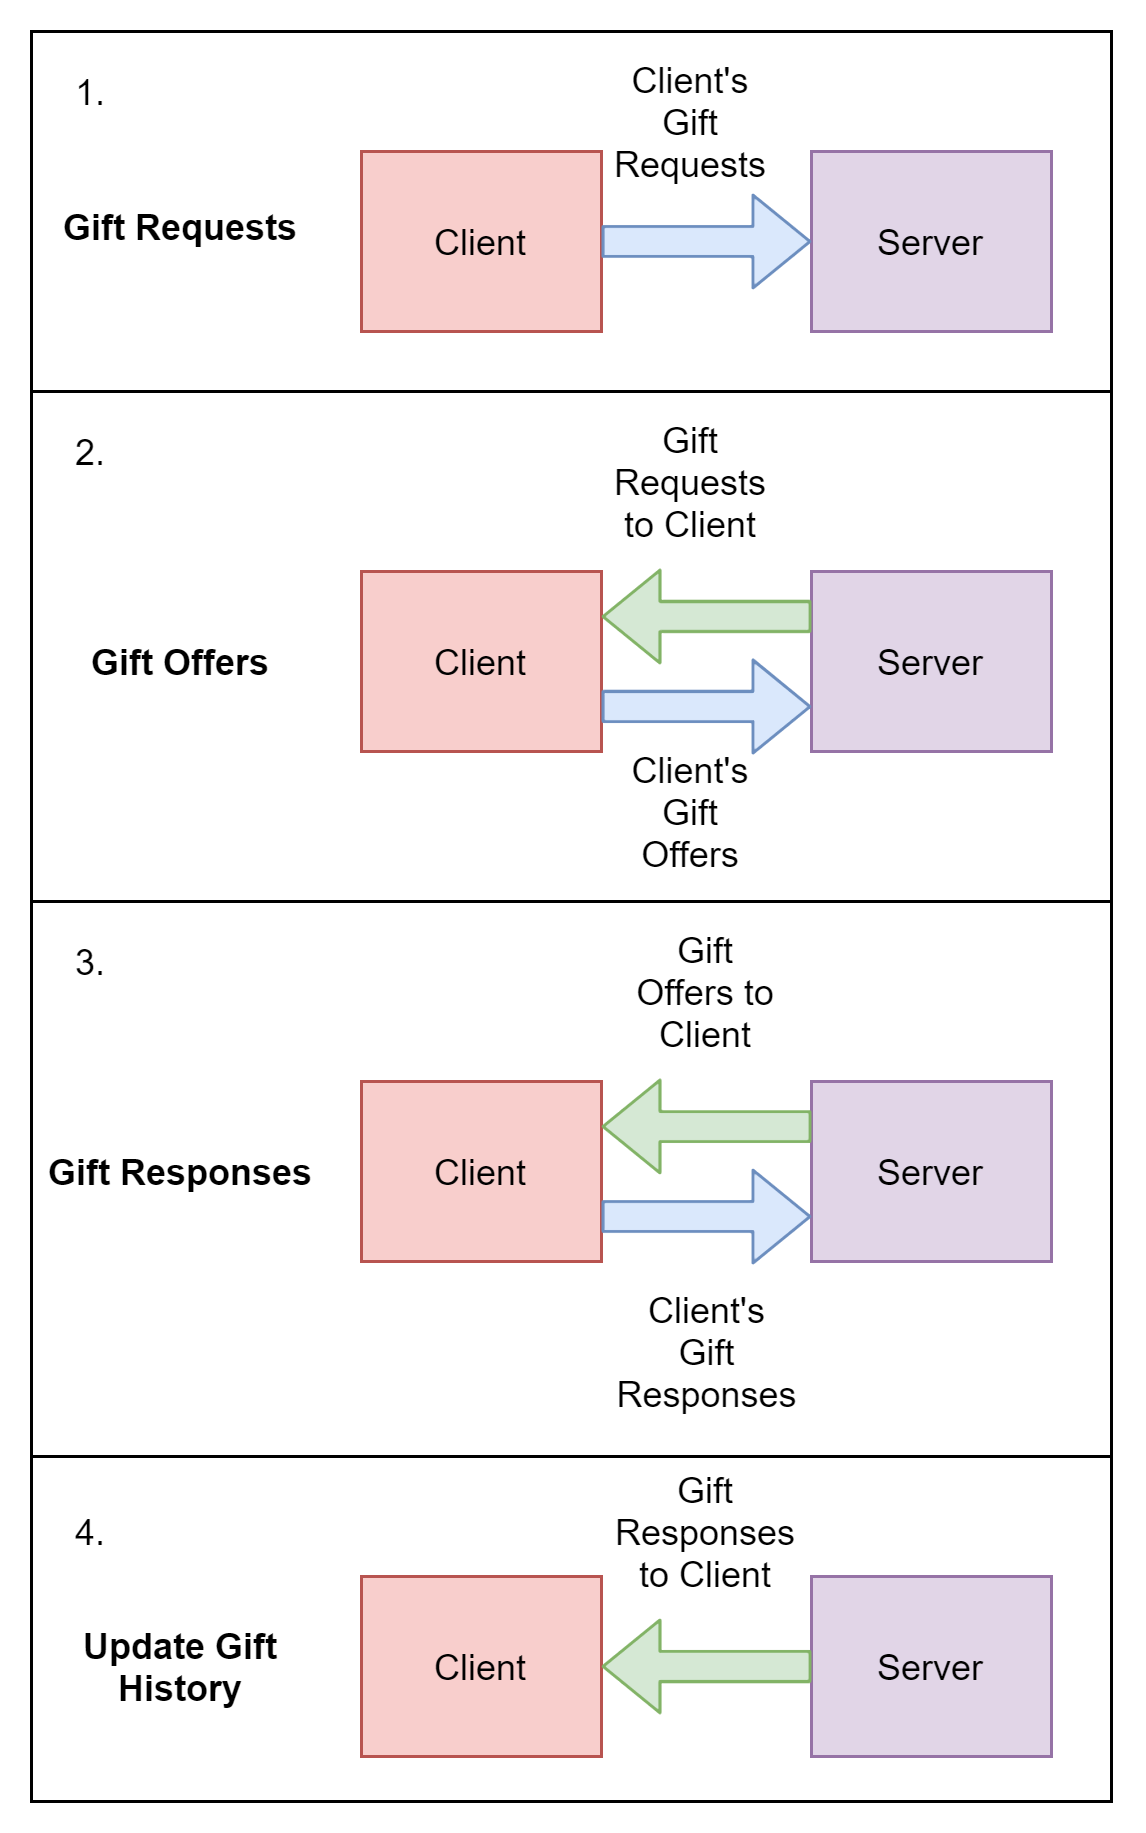
\includegraphics[width=0.6\textwidth]{06_iito/images/gifting_diagram.png}
    \caption{Overview of client-server interactions in gifting session.}
    \label{fig:IITO:gifting_session_diagram}
\end{figure}


    \chapter{Inter-Island Governmental Organisation (IIGO)}


The role of IIGO is to maintain, update, and revise the rules concerning provision to managing the long-term collective risk dilemma (ltCRD). 

\begin{itemize}
    \item There will be 3 distinct branches in the IIGO: the \textbf{legislative branch}, \textbf{executive branch} and \textbf{judicial branch}\footnote{This is, as no surprise, inspired by the separation of powers in Western democracies.}.
    \item Each role is put in power according to the  transfer-of-power rules (see Section~\ref{subsec:transfer-of-power} for more detail).
    \item The head of the legislative branch is the Speaker, the head of the executive branch is the President, and the head of judicial branch is the Judge.
    \begin{itemize}
        \item  The Speaker, President and Judge are selected, through a democratic election, from the islands in the archipelago\footnote{This naming is inspired by the roles in the US Government.}.
        \item The resources gathered by the archipelago are endogenous, hence acting on the institutional powers granted to the Speaker, President or Judge costs resources. 
        \item For their duty, the President, the Speaker and the Judge receive a salary for each of their turns in office (see Section~\ref{subsec:salary} for more detail).
        \item The limit of the powers of the President, Speaker and Judge are defined in this chapter (e.g. the Speaker can only call one vote per turn).
 
    \end{itemize}
\end{itemize}

\subsection{IIGO Specific Definitions}
\begin{definition} \label{def:ballot}
    A \textbf{ballot} is related to each island's \textbf{power} to support or disagree with the rule specified in the vote called by the President and to vote in favour or against an island for a specific role (i.e. the President, Speaker, Judge) at each round of the game.
\end{definition}


%\begin{definition} \label{def:vote}
    %A \textbf{vote} is related to a role's (i.e. the President, Speaker, Judge) \textbf{power} to call a vote for a specific rule or an election.
%\end{definition}


\begin{definition} \label{def:tax}
    The \textbf{taxation} is related to the President's \textbf{power} to request a specific \underline{\textbf{minimum}} amount of contribution from each island to the common pool at each round of the game. 
\end{definition}

\begin{definition} \label{def:alloc_req}
    An \textbf{allocation request} is related to each island's \textbf{power} to request a specific amount of resource allocation from the President at each round of the game.
\end{definition}


\begin{definition} \label{def:rule_prop_list}
A \textbf{rule proposal list} is related to each island's \textbf{power} to propose a specific rule to be passed to the President at each round of the game.
\end{definition}

\begin{definition} \label{def:invst}
    An \textbf{investigation} is related to the Judge's \textbf{power} to acquire information to make a decision, followed by a calculation of the expected results and checking whether some specific rules have been obeyed, exclusively for the actions carried out by the \textbf{islands}. 
\end{definition}


An example of an \emph{investigation}: The President has permitted the island $X$ to take the amount of $Y$ resources from the common pool. Upon \emph{investigation} carried out by the Judge, it is revealed that the amount of resources taken out from the common pool by the island $X$ is, in fact, $Y'$ such that $Y' \neq Y$.


\begin{definition}
\textbf{Monitoring} is a government official's \textbf{power} to perform event recognition and to check whether some specific rules have been obeyed.
\end{definition}

An example of \emph{monitoring}: The Speaker has performed only the following action: \emph{counted the votes and calculated the result} for a rule. Upon \emph{monitoring} carried out by the President, it is noticed that the Speaker has not made any \emph{announcement}. Hence, the Speaker has not followed their obligation to \emph{announce} the result of any vote held.

See Section~\ref{sec:accountability} for more information about which roles can monitor which ones.


\begin{definition}
\textbf{Investigative-monitoring} is a government official's \textbf{power} to acquire the information used in acting on a governmental power followed by calculation of the expected results and checking whether some specific rules have been obeyed, exclusively for the actions carried out by a government official they are responsible for.
\end{definition}

An example of \emph{investigative-monitoring}: The Speaker has performed the following actions: \emph{counted the votes and calculated the result $R$} for a vote $V$ and \emph{announced} the result $R'$ for the vote $V$. Upon \emph{investigative-monitoring} carried out by the President, it is noticed that $R' \neq R$. Hence, the Speaker has modified the announced result.


\begin{definition}
The \textbf{sanction} is related to the Judge's \emph{power} to punish non-compliant islands when their disobedience is confirmed through investigations at a specific turn.
\end{definition}


\begin{definition}
The (judicial) \textbf{pardon} is related to the Judge's \emph{power} to forgive a non-compliant island at a specific turn.
\end{definition}

\begin{definition}
The \textbf{budget} is the maximum amount of resources a role is permitted to spend from the common pool as it performs its own institutional-power-enabled actions at a specific turn.
\end{definition}


\begin{definition}
The \textbf{salary} is the amount of resources a role is to be given from the common pool as a reward for performing its institutional-power-enabled actions at a specific turn.
\end{definition}

\begin{definition} \label{def:term}
A \textbf{term} is the number of turns an island is \emph{permitted} to hold a role, and after which the responsible role (indicated in the transfer-of-power cycle in Figure~\ref{fig:cycles_in_IIGO}) is \emph{obliged} to initiate transfer-of-power.
\end{definition}

\subsection{\emph{Power}, \emph{Permission} and \emph{Obligation} Distinction}
In the rest of the specifications, we will be specifically using the following three terms to define the actions and responsibilities carried out by the Speaker, President, Judge (see Figure~ \ref{fig:per_obl_sets}):
\begin{itemize}
    \item Power
    \item Permission
    \item Obligation
\end{itemize}



\begin{figure}[H] 
\centering
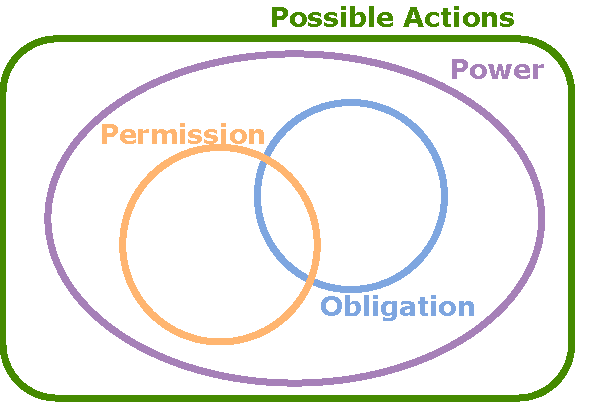
\includegraphics[width=0.6\textwidth]{05_iigo/images/SOMAS_per_obl.pdf}
\caption{Relationship between \emph{power}, \emph{permission} and \emph{obligation}.}
\label{fig:per_obl_sets}
\end{figure} 


For example, the Judge has the \emph{power} to carry out investigations at an IIGO session. There are no rules specifying which specific islands the Judge should investigate. Therefore, the Judge has the \emph{permission} to investigate any `alive' islands during a session. However, the Judge is \emph{obliged} to make at least some number of investigations each turn.



\section{Executive Branch}
\label{sec:executive}
The executive branch is responsible for \textbf{carrying out the law}.
\begin{itemize}
       
    \item The President has the \emph{power} to: 
    \begin{itemize}
        
        \item Select a rule for voting $R^{*}$ to be passed to the Speaker.
        \begin{rule_IIGO}
            The President has the \emph{obligation} to \emph{select} a rule $R^{*}$ if the \emph{rule proposal list} has at least one proposed rule in it.
        \end{rule_IIGO}
        \begin{rule_IIGO}
            The President has the \emph{permission} to \emph{select} a rule $R^{*}$ if and only if $R^{*} \in S$, where $S$ is the \emph{rule proposal list}.
        \end{rule_IIGO}
        
        \item Decide the amount of individual \emph{taxation} (i.e. a specific \emph{minimum} amount of contribution to the common pool for each island) for the current turn.
        
        \begin{itemize}
            \item The President is given the self-reported resource amounts held by each island to assist in this decision.
            %\item Suggested Rule: For any island that has chosen to not report it's resources, the President has the \emph{obligation} to set them an individual tax amount T.
        \end{itemize}
        
        \item Decide the allocation of resources distributed from the common pool to the islands (i.e. a specific \emph{maximum} amount an island is permitted to take from the common pool).
        
        \begin{itemize}
            \item The President is given the \emph{allocation requests} made by each island.
            %\item \emph{}{Suggested Rule:} The President has an obligation to prioritise islands in critical condition.
        \end{itemize}
    \end{itemize}
\end{itemize}



\section{Legislative Branch}
\label{sec:legislative}
The legislative branch is responsible for \textbf{making the law}.
\begin{itemize}

    \item The Speaker has the \emph{power} to:
    \begin{itemize}
        
        \item Call a vote $V$ for a rule $R$.
        \begin{rule_IIGO}
            The Speaker has the \emph{obligation} to \emph{call} a vote $V$ if and only if the President has \emph{selected} a rule $R$ to be voted on.
        \end {rule_IIGO}
        \begin{rule_IIGO}
            The Speaker has the \emph{permission} to \emph{call} a vote $V$ for a rule $R$ if and only if the rule $R = R^{*}$, where $R^{*}$ is the rule \emph{selected} by the President.
        \end {rule_IIGO}
            
        \item Choose which islands are participating in the vote $V$.
       % \footnote{This is our sequential implementation alternative for the power to close the ballot box.}.
        \begin{rule_IIGO}
            The Speaker has the \emph{obligation} to ask for a vote from all alive islands.
        \end {rule_IIGO}
            
        \item Declare the result $C$ of a vote $V$. 
        \begin{rule_IIGO}
            The Speaker has the \emph{obligation} to \emph{declare the result} $C$ for a vote $V$ if and only if the vote V has been \emph{called}.
        \end {rule_IIGO}
        \begin{rule_IIGO}
            The Speaker has the \emph{permission} to \emph{declare the result} $C$ for a vote $V$ if $C = C^{*}$, where $C^{*}$ is the result produced by \emph{calling} the vote $V$.
        \end {rule_IIGO}
        \begin{itemize}
            \item This step is what enables a rule to be \emph{active}.
        \end{itemize}
    \end{itemize}
\end{itemize}




\section{Judicial Branch}
\label{sec:judicial}

The judicial branch is responsible for \textbf{evaluating the law}.
\begin{itemize}
    \item The Judge has the \emph{power} to:
    \begin{itemize}
        \item Perform a number of \emph{inspections}\footnote{An \emph{inspection} \textbf{costs} an expense of resources (See Definition~\ref{def:invst} for more detail).} $I$ and produce a compliance outcome $\mathbb{O}^{*}$\footnote{Note that the compliance outcome $\mathbb{O}^{*}$ considered is a boolean.}.
        %(true: the island has been compliant with the rules in play, false: the island has not been compliant with the rules in play)
        %\begin{itemize}
           % \item For example, to check if the event outcome is \emph{concurrent}\footnote{Again, what is defined as "concurrent"? A clear definition is needed.} with the rules.
        %\end{itemize}
        \begin{rule_IIGO}
            The Judge has the \emph{obligation} to make at least $N$ investigations at each turn.
        \end{rule_IIGO}
        \item Declare the outcome $\mathbb{O}$ of an inspection $I$ to all islands\footnote{This act of broadcasting is especially important for islands to form an opinion about the sanctioned islands accordingly.}.
        \begin{rule_IIGO}
            The Judge has the \emph{obligation} to declare the outcome $\mathbb{O}$ of an inspection $I$ if and only if the inspection $I$ has been performed.
        \end{rule_IIGO}
        \begin{rule_IIGO}
            The Judge has the \emph{permission} to declare the outcome $\mathbb{O}$ of an inspection $I$ if $\mathbb{O} = \mathbb{O}^{*}$, where $\mathbb{O}^{*}$ is the outcome of the inspection $I$.
        \end{rule_IIGO}
        %\item Initiate the removal of the \texttt{President}.
        %\begin{itemize}
            %\item A good Judge would be especially vigilant during \emph{power transfer} regarding the \emph{President} position (see Section~\ref{leg_const} for more detail).
        %\end{itemize}
        \item Invoke economic \textbf{sanctions} (see Section~\ref{sec:sanctions} for more detail).
        \begin{rule_IIGO}
            The Judge has the \emph{obligation} to invoke a sanction $S$ for an island $X$ if and only if an investigation $I$ has an outcome $\mathbb{O}^{*}$ indicating non-compliance, and $I$ is an investigation of an action taken by island $X$.
        \end{rule_IIGO}
        \item Invoke even more severe sanctions in the case of further disobedience to previous sanction(s).
        \begin{rule_IIGO}
            The Judge has the \emph{permission} to invoke a severer sanction $S'$ for an island $X$ if the island $X$ has not fulfilled the requirements of the previous sanction $S$.
        \end{rule_IIGO}
        \item Pardon the islands which are currently sanctioned.
        \begin{rule_IIGO}
            The Judge has the \emph{permission} to revoke any sanction $S$ of an island $X$ at a specific turn.
        \end{rule_IIGO}
    \end{itemize}
\end{itemize}
%(e.g. a new rule that falls under a "sanction" category \hl{[I'm not sure about this being a `new rule` [Ezgi]]}

\subsection{Sanctions}
\label{sec:sanctions}
All sanctions are of economic nature which include:
        \begin{itemize}
            %\item Revoking an island's access to the common pool.
            \item Enforcing an island to contribute a specific amount of resources to the common pool.
            \begin{itemize}
                \item This does not mean that the Judge has the \emph{power} to take resources from an island in order to put them to the common pool -- the island itself is expected to carry out this implication imposed by the sanction itself, otherwise further punishment can be induced by the Judge.
                \item Similarly, \emph{opinion formulation} will follow accordingly whether the island(s) is/are following the implications imposed by the sanction(s).
            \end{itemize}
        
    \end{itemize}
    Sanctions are the associated penalty that comes with an island breaking a specific rule. The Judge is in full control of the penalties associated with breaking any rules. Once the Judge has specified the score of the penalty associated with each time an island breaks a rule, the cumulative penalties accumulated by the island are then used to determine which \textbf{sanction tier} that each island falls into. The score threshold to determine the boundaries of the sanction tiers are set by the Judge. At each turn of the game, each island is told whether they are being sanctioned, and if so, which \textbf{sanction tier} that they are currently in. The \textbf{sanction tiers} of the non-compliant islands are also broadcasted to the other islands in the archipelago. To summarise, the sanctioning process follows these steps:
    
    
    
    %Sanctions are based on an island breaking a rule. Each rule must therefore have an associated penalty. By default, we set these penalties such that they add $1$ to the total sanction score for each island. However, we allow the judge to override this scoring, the judge is able to set their own scores for any particular rule as they desire. This custom scoring is then used when an island breaks a particular rule. By looking at events that occurred in the last turn, and using the customised scoring we provide the holder of the judge role with full control of the penalties for breaking any rules.
    
    





%we then use the cumulative penalties accumulated by each island to determine which Sanction Tier they fall into. The score threshold's required to fall into these sanction tiers is set by the judge and is checked for monotonicity. Each island is told whether they are being sanctioned, and is so what tier they are in. We also tell other islands about which sanction tiers other islands have fallen into. 

    \begin{enumerate}
        \item The Judge has the \emph{power} to set custom penalties associated with breaking any rules.
        \item The Judge is given a list of all events that occurred in the previous turn.
        \item The Judge has the \emph{power} to check whether any, or all of these previous events, involve the islands in the archipelago breaking any rules.
        \item Each of the transgressions is scored using the Judge's custom penalties if the Judge has set them. Otherwise, a score of $1$ is given each time a rule is broken.
        \item The Judge has the \emph{power} to revise the sanction thresholds.
        \item Using the latest sanction thresholds available, each island is assigned to a sanction tier based on the sanction score that it has received.
        \item These sanction tiers are broadcasted to all of the islands in the archipelago.
        \item The Judge then uses sanctions rules in place to calculate the specific amount of resources that each non-compliant island has in order to determine how much it should contribute to the common pool, based on the sanction tier that it is in.
    \end{enumerate}



\section{Constitutional Rights and Obligations in the Archipelago}
\label{sec:const_rights_obl_archi}
Each island has the \emph{power} to:
\begin{itemize}
\item make an \emph{allocation request} (see Definition~\ref{def:alloc_req}) to the President for a specific amount to be allocated to them.
\item report the number of resources it is in possession of to the President.
\begin{rule_IIGO}
    Each island has the \emph{obligation} to report the number of resources it is in possession of to the President.
\end{rule_IIGO}
\begin{rule_IIGO}
    Each island has the \emph{permission} to report the number of resources $R'$ if and only if $R' = R$, where R is the number of resources the island is in possession of.
\end{rule_IIGO}
\item take resources from the common pool.


\begin{rule_IIGO}
    Each island has the \emph{permission} to take at maximum $N$ resources, where $N$ is the specific allocation made by the President to that island\footnote{If no such allocation is made, the island is \emph{permitted} to take any amount of resources.}.
\end{rule_IIGO}
\item contribute resources to the common pool.
\begin{rule_IIGO}
    Each island has the \emph{obligation} to contribute to the common pool an amount greater or equal to that of the individual tax set by the President.
\end{rule_IIGO}
                %The President is in
                %(unless there is a rule in place that dictates how Speaker is to allocate resources).
\item add a rule to the \emph{rule proposal list} (see Definition~\ref{def:rule_prop_list}) at the start of each turn.
        %\begin{itemize}
            %\item The game specification includes how many rules an island can propose each turn.
        %\end{itemize}
        %\item vote  for rules in the Legislative Branch and vote for their favourite islands in elections
\item participate in the legislative branch of the government by casting ballots in votes called by the Speaker
\item vote for an island to be elected for a specific role (e.g. the President, Judge, Speaker) during the elections\footnote{This will be assumed to be true \underline{unless stated otherwise}. %Note that \textbf{diplomatic sanctions} can disable this power of a specific island (see Section~\ref{jud_const}).}.
        }.
\end{itemize}
\section{Accountability Cycle}
\label{sec:accountability}


To ensure that the government avoids corruption and abuse of power, each branch is accountable to another. The President is accountable to the Speaker, the Speaker is accountable to the Judge, and the Judge is accountable to the President (see Figure~ \ref{fig:cycles_in_IIGO}). This accountability cycle is enacted through \emph{monitoring} actions\footnote{Note that the terms \textbf{monitoring} and \textbf{investigation} have similar but quite different meanings in the IIGO context.}. 

The powers related to the accountability cycle and transfer-of-power for each role can be summarized as the following: 
\begin{itemize}
    \item The Speaker has the \emph{power} to: 
    \begin{itemize}
        \item monitor the President.
        \item announce the result of this monitoring.
        \item initiate the transfer-of-power for the Judge.
    \end{itemize}
    \item The President has the \emph{power} to: 
    \begin{itemize}
        \item monitor the Judge.
        \item announce the result of this monitoring.
        \item initiate the transfer-of-power for the Speaker.
    \end{itemize}
    \item The Judge has the \emph{power} to: 
    \begin{itemize}
        \item  monitor the Speaker.
        \item announce the result of this monitoring.
        \item initiate the transfer-of-power for the President.
    \end{itemize}
\end{itemize}

%Unlike investigations performed by the Judge, who performs investigations on island actions in the following turn, each role is given the opportunity to check up on the actions of the role it is responsible for immediately after they have been performed. In this sense, the President can monitor (includes investigative-monitoring) the powers (calling a vote and announcing the result) acted on by the Speaker immediately after the Speaker's announcement (or lack there of). The government officials hold a lot of power so this is to ensure that any wrong-doing is determined as quickly as possible. For this project we are only pursuing one degree of monitoring, that is, the powers relating to the accountability cycle will not be monitored themselves. We assume that agents will act in the interest of themselves and keeping all the islands alive is beneficial to everyone. Hence, while the agents might be inclined to break rules in order to benefit themselves, anyone else breaking the rules is seen as undesirable under the assumption that the system in place is there to benefit all. 


Through the proposed accountability cycle, each role is given the opportunity to check up on the actions of the role it is accountable for immediately after they have been performed. It is clear that the IIGO roles (i.e. the President, Speaker and Judge) hold a considerable amount of \emph{power} in their hands. The accountability cycle is designed to address the possible abuses of this power. With monitoring, any wrong-doing in the IGO is determined as quickly as possible and the role in question can be replaced. 

Within the scope of the coursework, we decided to pursue only \emph{one degree of monitoring}, meaning that the powers relating to the accountability cycle will not be monitored themselves. We assume that agents will act in the interest of all the islands in the archipelago. Hence, while the agents might be inclined to break the rules to benefit in some form, it is assumed that the others will negatively see any non-compliant islands based on the assumption that the proposed IIGO system is in place to maintain the welfare of all the islands.

Let role $X$ be accountable to the role $Y$, which is accountable to the role $Z$. Then:
\begin{rule_IIGO}
$Y$ has the \emph{obligation} to declare the outcome of the monitoring result $M$ associated with the action $A$ undertaken by $X$ if and only if $Y$ has monitored the action $A$ performed by $X$. 
\end{rule_IIGO}
\begin{rule_IIGO}
$Y$ has the \emph{permission} to declare the monitoring result $M$ associated with the action $A$ undertaken by $X$ if and only if $M = M^{*}$, where $M^{*}$ is the outcome of \emph{monitoring} action $A$ performed by $X$\footnote{These constitutional rules should be available to the agents to check their decision against. However, due to having only one degree of accountability cycle in place, these rules are not enforced through any sanctions (i.e. breaking these rules has no consequences as they only deem to be an \emph{agreement} among the roles).}.
\end{rule_IIGO}


\begin{figure}[!htb]
\centering
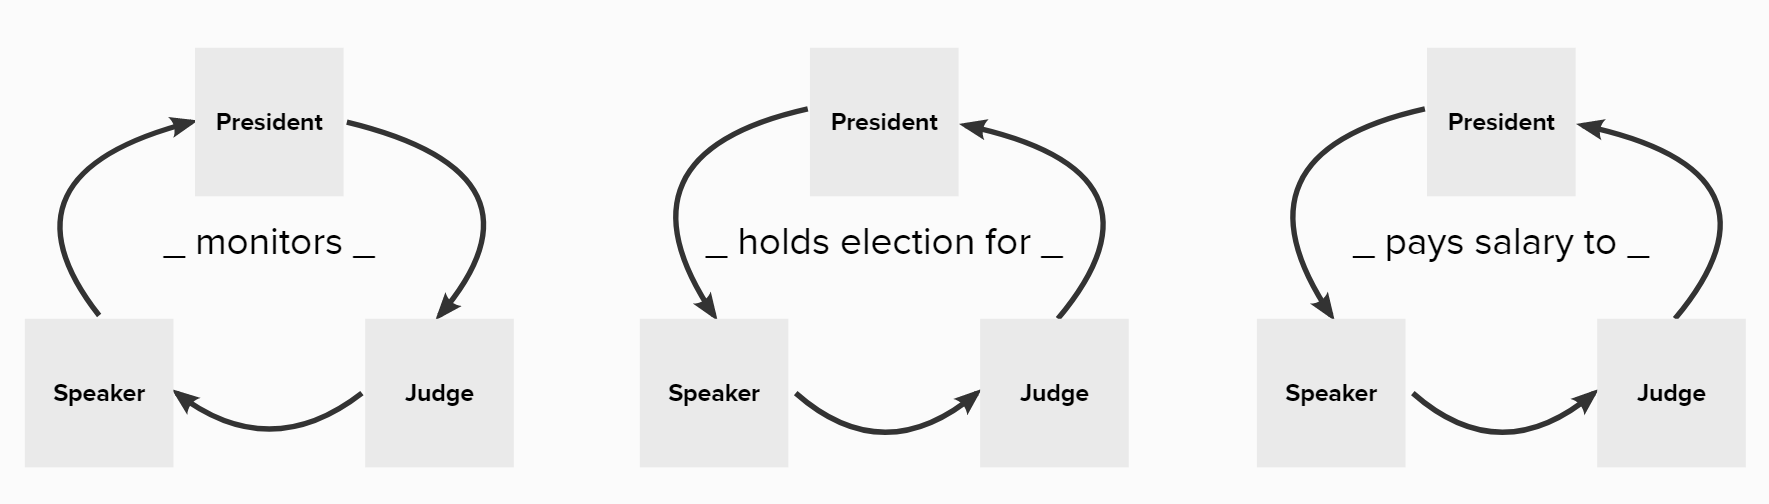
\includegraphics[scale=0.33]{05_iigo/images/role cycles.png}
\caption{Accountability cycle (left), the transfer-of-power cycle (middle) and salary cycle (right).}
\label{fig:cycles_in_IIGO}
\end{figure}


\subsection{Transfer-of-power}
\label{subsec:transfer-of-power}
\begin{enumerate}
    \item The Speaker conducts a vote for the election of the new Judge.
    \item The Judge conducts a vote for the election of the new President.
    \item The President conducts a vote for the election of the new Speaker.
\end{enumerate}
Refer to the Figure~ \ref{fig:cycles_in_IIGO} for further clarification about the transfer-of-power cycle.

\begin{rule_IIGO}
   The role $X$ has the \emph{obligation} to conduct a vote for the election of $Y$ at the end of the term (see Definition~\ref{def:term}) if and only if the role $X$ is accountable to the role $Y$. 
\end{rule_IIGO}.

\section{Budget and Salary}
\subsection{Budget}
%Actions associated with the IIGO have an associated cost that is defined as a configuration parameter. The institutional-power-enabled actions of  identified to require a "computational" component are:

Institutional-enabled-power actions in the IIGO have an associated cost with them. Some examples for such actions include:


%that is defined as a configuration parameter. The institutional-power-enabled actions of  identified to require a "computational" component are:


%We have defined the resource to be an endogenous one, hence any computation surrounding the distribution of the resource must use up some of that resource. 
\begin{itemize}
\item Calling any vote and computing the winner.
\item Declaring (e.g. \textit{announcing} the result of a vote).
\item Setting the amount of \emph{taxation} for each island.
\item Deciding the allocation distribution for each island.
\item Inspecting an island's action history.
\item Monitoring a role.
\end{itemize}

Since IIGO has been designed to act in the common good, IIGO-related costs will be directly withdrawn from the common pool. Since the common pool is considered a communal property of the archipelago, there are rules in place to limit how much each role is allowed to spend in order to perform its own institutional-power-enabled actions. This is the reason why defining the \emph{budget} and keeping it separate for each of the three IIGO roles.


As a role performs institutional-enabled-power actions, the corresponding cost associated with this action is subtracted from the role's budget. A budget of zero means that the role does not have the \emph{power} to perform any of its institutional-power-enabled actions. The removal of the budget rule from the rules in play means the role is allowed to perform as many such actions as it prefers to (as long as those actions are not governed by other rules). 



%As a role performs an endogenous-cost action, the corresponding cost associated with this action is subtracted from the role's budget. Thus, if as a result of an endogenous-cost action a role will be left with negative budget, it will have gone over the budget limit and will have broken the budget rule. A budget of zero means that the role is not allowed to perform any of its institutional-power-enabled actions associated an endogenous-cost. The removal of the budget rule from the rules in play means the role is allowed to perform as many such actions as it pleases (as long as those actions are not governed by other rules). 

The budget rule is also persistent across turns. This means that, assuming nothing else affects the budget, if a role has $100$ resources in its budget at each turn and spends only $10$ resources, this means that this very same role has $90$ resources in its budget at the next turn. On the other hand, islands can choose to increase the budget periodically every turn. This is governed by another budget extension rule.




%one turn and it spends 10, it has 90 resources in it's budget the next turn. 

Finally, it must be noted that the budget is inherently linked with the fact that whether obligations of a specific role can be undergone.
For example, during \emph{monitoring}, it should not be seen as a rule violation if a role has not acted on an obligation if it would go over the budget as a result. 

%This can also be seen as an added clause "... and the action is only permitted if they have the budget" to most rules which govern actions with an endogenous-cost.
%\begin{rule_IIGO}
    %The budget is increased by an amount $N$ every turn.
%\end{rule_IIGO}

%This rule means that, assuming nothing else affects the budget, if a budget is set to increase by 10 resources every turn and the budget is a 100 resources in turn one, the budget is 110 resources in turn 2. Setting this rule to 0 is equal to removing this rule and it means that the budget is never increased. 


\subsection{Salary}
\label{subsec:salary}
A salary is paid to each role in power as an incentive to act in a publicly approved way. %Hence, each role has the \emph{power} to pay a salary to another role following the salary cycle in Figure~\ref{fig:cycles_in_IIGO}.
\begin{rule_IIGO} \label{rule:salary}
   %Each role has the \emph{obligation} to pay the salary of amount $S$ to another if and only if the amount paid $S'$ is equal to $S$.
   Each role has the \emph{obligation} to pay the salary of amount $S$ to one another following the salary cycle in Figure~\ref{fig:cycles_in_IIGO}.
\end{rule_IIGO}

In Rule~\ref{rule:salary}, setting $S=0$ (through changing the active rules in place) means that roles do not have the permission to pay any salary. Removing the Rule~\ref{rule:salary} means that the roles may freely choose the amount $S$ for the salary payments.

\section{IIGO Session order}

\begin{enumerate}
    \item The Judge has the \emph{power} to check the history of actions to confirm whether the previously punished island(s) has/have obeyed the previous round's sanctions, meaning whether they contributed to the common pool accordingly in case of economic sanctions.
    %\begin{itemize}
      %  \item \emph{Suggested Rule:} In case of disobeying sanctions, the Judge is \emph{obliged} and \emph{permitted} to increase the severity of sanctions with respect to specific islands.
   % \end{itemize}
    \item The Judge has the \emph{power} to carry out \emph{inspections} on the history of actions of any island $X$ to check whether:
        \begin{enumerate}
        \item the reported resources of $X$ in the previous round match the real value of resources $X$ had in its private pool for the previous turn.
        \item the island $X$ has retrieved the right amount of the resources from the common pool, based on the \emph{allocation request} evaluated by the previous President.
            \begin{itemize}
            \item An example: In the previous round, the President has decided that the island $X$ can take $Y$ amount of resources from the common pool. If the Judge finds out that the island $X$ has taken an amount of $Y'$ such that $Y' > Y$, the Judge has the \emph{power} to invoke sanctions on the island $X$.
            
            %the Judge is \emph{obliged} and \emph{permitted} to sanction island $X$.
            \end{itemize}
        \end{enumerate}
    \item The Judge has the \emph{power} to invoke sanctions based on the outcome of the inspections.
    \item The President has the \emph{power} to decide to carry out a \emph{monitoring} on:
        \begin{enumerate}
        \item the sanctions imposed by the Judge.
        \end{enumerate}
    \item The islands may report the resources in their private pools to the President.
    \item The President has the \emph{power} to let each island know about the amount of \emph{taxation} they have to pay.
    \item The island has the \emph{power} to make an \emph{allocation request} to the President.
    \item The President has the \emph{power} decide on an allocation of resources and let each island know about the amount of resource allocation they are permitted to take from the common pool.
    \item The island has the \emph{power} to pick and to propose a rule to be voted on to the President.
    \item The President has the \emph{power} to choose a rule to be voted on from the received rule proposals.
    \item The Speaker has the \emph{power} to decide to carry out a \emph{monitoring} on: 
        \begin{enumerate}
        \item the resource allocation decided by the President.
        \item the rule proposed by the President.
        \end{enumerate}
    \item The Speaker has the \emph{power} to call a vote.
        \begin{enumerate}
        \item The islands vote in support of, or against, the rule (aye or nay) anonymously.
        \end{enumerate}
    \item The Speaker has the \emph{power} to announce a result of a vote to the islands and carries out the law change, if required (e.g. deleting/rejecting a rule if there is a majority nay vote).
    \item The Judge has the \emph{power} to decide to carry out \emph{monitoring} on:
        \begin{enumerate}
        \item the vote called by the Speaker.
        \item the Speaker announcing the result.
    \end{enumerate}
    \item The roles pay salary for one another following the accountability cycle in Figure~ \ref{fig:cycles_in_IIGO}.

\end{enumerate}



\section{Future Work}

\begin{itemize}
    \item \textbf{Diplomatic sanctions}: Although having the potential of being a good alternative for severer sanctions discussed in  Section~\ref{sec:sanctions}, diplomatic sanctions are \emph{not} implemented within the scope of the coursework. \\
    Suggested diplomatic sanctions include:
        \begin{itemize}
            \item Revoking an island's eligibility to vote and to be elected for a position.
            \item Revoking an island's eligibility to propose a rule/motion.
        \end{itemize}
    \item \textbf{Immutable rules}: Within the scope of the coursework, a subset of rules could have been categorised as immutable. This means that to change such immutable rules, the islands first need to vote to change their status to be \emph{mutable}, and consequently, hold another vote to change these mutable rules.
    %\item \textbf{Adding rules to the proposal list: } 
\end{itemize}

    \chapter{Voting}
\section{Voting Scenarios}
\label{sec:VotingScenarios}

Within the context of the coursework, robust voting systems were designed to determine the outcome of collective actions (e.g. elections for legislative, executive and judicial branches in IIGO).
When voting is called in the IIGO, the President, Speaker, Judge and the islands in the archipelago (i.e. the \emph{Voters}, assuming that no diplomatic sanction is in place) will be empowered to proceed with the following series of actions:
\begin{itemize}
    \item The President will be eligible to select a rule for the archipelago to vote for.
    \item The Speaker will be eligible to take charge of enabling the voting procedure by receiving, counting ballots and ultimately, declaring the winner.
    \item The islands in the archipelago (i.e. Voters) will be eligible to vote by submitting their ballots\footnote{This is based on the assumption that no diplomatic sanctions are in place for any islands.}.
\end{itemize}

In an IIGO session, the voting action is needed to decide the next President, Speaker, Judge and also to decide whether or not to adapt a new rule as well as to disable an active one.

\textbf{Elections of IIGO roles:} As per the IIGO specification, the elections of roles will be conducted according to the accountability cycle (see Section XX): The Judge can initiate the transfer-of-power for the Speaker; the President can initiate the transfer-of-power for the Judge; the Speaker can initiate the transfer-of-power for the President. To prevent multiple-role enactment of the same island, the island that has been selected for a role will be removed from the candidate list for other roles in the current turn\footnote{Note that this assumes that the following rule is in place: The President, Speaker and Judge are all different islands.}. Depending on the sequence of the elections called, the candidates for three roles will consist of maximally six, five, and four islands accordingly. The ballots from the Voters will be in the format of preference lists which rank all candidates in the desired order.

\textbf{Changes of rules:} The President has the power to select a rule from the \emph{rule proposal list} to be voted by the Voters. The Speaker will host the voting for this rule and will be responsible for counting the votes in order to declare the result. The votes from the Voters can only be of the following types: \textbf{Aye} (namely agree with the rule change), \textbf{Nay} (namely disagree with the rule change) or \textbf{Abstain}.


\section{Voting Methods}
\label{sec:VotingMethods}

\begin{table}[H]
\caption{Available voting methods for each voting scenario}\label{table:votingmethod}
\begin{center}
\begin{tabular}{ |p{3cm}||p{3cm}|p{3cm}|  }
 \hline
 Voting Methods   & Elections of Roles & Changes of Rules   \\
 \hline
 Plurality   &     & \checkmark     \\
 \hline
 Borda Count &  \checkmark   &      \\
 \hline
 Runoff      &  \checkmark    &        \\
 \hline
 Instant Runoff    & \checkmark  &     \\
 \hline
 Approval  &  \checkmark    &    \\
 
 \hline
\end{tabular}    
\end{center}
\end{table}

Table \ref{table:votingmethod} indicates the available voting method choices for each voting scenario considered in the coursework.

\textbf{Plurality} will select the relative majority choices as the collective decision. The Plurality voting method will be used to decide whether a change of rule goes into effect in an IIGO session. When the number of valid ballots (i.e. abstention excluded) is odd, the Plurality method can determine the winner without tied results. Otherwise, the solution to tied results is regimented with the assumption that the proposer of the voting in such events will vote for "agree". Thus, the proposal will be approved if the number of "agree" votes is more than the number of "disagree" votes. 

\textbf{Borda Count} method will allow Voters to rank their preference instead of choosing \emph{only} one option. The order of choices in the preference list determines the Borda points regarding each option. Adding such Borda points from all votes produces the Borda score for each candidate. Thus, the candidate with the highest Borda score will be the winner.

\textbf{Runoff} (also known as the two-round system) is a voting method that counts the ballots for two rounds. Voter islands will rank their preference of candidates and submit the preference lists as their ballots. In the first round, candidates with the top most and second most first-place votes are chosen among all candidates. If one of them obtains a majority, the Runoff method can conclude this candidate to be the winner. Otherwise, the second round will proceed where the ballots will be recounted by eliminating the candidates other than the top two choices. Subsequently, the candidate with the most votes between the top two candidates will be the winner.

\textbf{Instant Runoff} is a voting method used in elections for a single seat, that consist of more than two candidates.
Individual voters rank their preference of candidates. The candidate who gets the least number of first-place is eliminated, and this step is repeated until only one candidate remains.

\textbf{Approval} is a voting method for a single winner in which each voter selects a subset of candidates. Approval will be used for the elections of roles where each voter picks a group of candidates, and the most named or approved candidate wins.

In case of a \textbf{tied election}, three possible rules can eliminate one or more candidates who get the same number of votes:
\begin{itemize}
    \item The Condorcet method is one of the voting methods which selects the candidate that dominates other candidates in terms of majority relation which ranks the candidates according to one-to-one comparisons. In other words, the Condorcet winner is the candidate that wins a majority in every one-to-one comparison against other candidates. However, the Condorcet method is not guaranteed to work when preference lists form a cycle, which is known as the Condorcet paradox.
    \item Hare Rule can be used in a tiebreak where all candidates with the least first-place votes will be all eliminated.
    \item Coombs Rule can be used in place of Hare Rule if the iterative process of removing candidates with the least first-place votes is not preferred. Coombs Rule states that the candidate with the most last-place votes will be removed.
\end{itemize}

In this coursework, the pairwise Condorcet winner is chosen as a tiebreaker which states that a candidate who dominates the other candidate in terms of majority relation wins.

\section{Voting Protocol}
\label{sec:VotingProtocol}
The suggested voting protocol is adapted from an example of formal specification given in Robert's Rules of Order (RONR) that defines a series of sequential actions when a voting event happens.

This protocol is applicable to any voting method at a certain state of the game.

When a voting event happens, the sequence of actions of the voting protocol in this game is:
\begin{itemize}
    \item The President selects a rule from the rule proposal list to be voted on.
    \item The President notifies the Speaker to hold a voting event for the selected rule.
    \item The Speaker calls for a vote for the selected rule by opening ballots to all islands to cast their votes.
    \item The Speaker closes the ballots after receiving votes from all islands.
    \item The Speaker counts the votes by calling an applicable voting method function for winner selection to produce a result.
    \item The Speaker publicly declares the voting result whether the selected rule can be carried out or not.
\end{itemize}

Figure~\ref{fig:RONRVotingProtocol} shows the sequence of the voting protocol for changing and/or adapting a new rule.

\begin{figure}[!htb]
\begin{center}
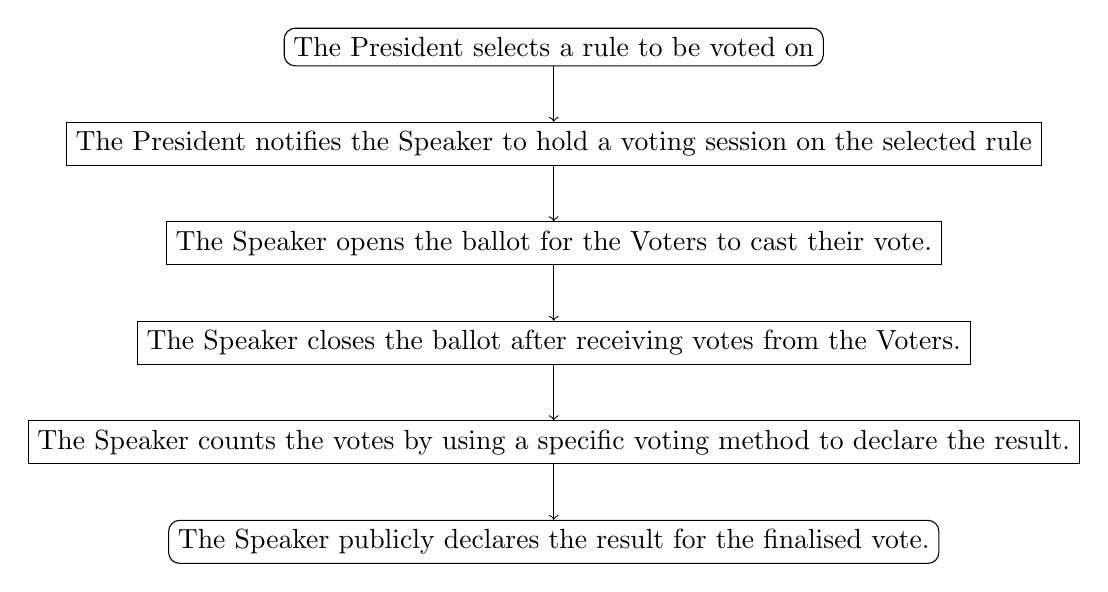
\begin{tikzpicture}[node distance=20pt]
\centering
\node[draw, rounded corners] (start)  {The President selects a rule to be voted on};
\node[draw, below=of start] (step 1)  {The President notifies the Speaker to hold a voting session on the selected rule};
\node[draw, below=of step 1] (step 2)  {The Speaker opens the ballot for the Voters to cast their vote.};
\node[draw, below=of step 2] (step 3)  {The Speaker closes the ballot after receiving votes from the Voters.};
\node[draw, below=of step 3] (step 4)  {The Speaker counts the votes by using a specific voting method to declare the result.};
\node[draw, below=of step 4, rounded corners] (end)   {The Speaker publicly declares the result for the finalised vote.};
 \draw[->] (start)  -- (step 1);
 \draw[->] (step 1) -- (step 2);
 \draw[->] (step 2) -- (step 3);
 \draw[->] (step 3) -- (step 4);
 \draw[->] (step 4) -- (end);
\end{tikzpicture}
\caption{Voting Protocol for Rules}
\label{fig:RONRVotingProtocol}
\end{center}
\end{figure}

For elections of roles, the sequence of actions of the voting protocol is mostly similar to the above explanation in principle, except for some parameters, such as the motion of the vote which is the role itself (President, or Speaker, or Judge), the facilitator of the election/vote event which depends on what role is being held for election (refer to Chapter 5 IIGO for more details on change of roles and power transfer), and the applicable voting method function to call for election that will produce the result, which is different from the voting method used for rules. Refer to Section~\ref{sec:VotingMethods} for more details on voting methods to be used for elections of roles.

At the start of the game, it is assumed that all 6 islands have the power to vote at any necessary voting scenario, and no diplomatic sanction is in place for any island. However, in the further turns of the game, some island(s) could lose their right to vote and/or not permitted to participate in a voting event due to the diplomatic sanction(s) in place. Refer to Chapter 5 IIGO for details on diplomatic sanction. In this case, the Speaker will open the ballots to the eligible islands only , i.e. those who are permitted to vote at a certain state of the game.

% Implmentaion section deleted

    \chapter{Team 1 Agent Design}

\section{Core Idea}
Team 1 agent was designed around the idea that the agent wants the whole archipelago to survive. However, the agent does have different configurations to allow for some malicious behaviour in order to facilitate some interesting agent interactions.

\section{Emotional state}

The agent's behaviour is affected by what we have termed her \emph{emotional state}. This is governed by the agent's current resources in relation to the living cost.

\begin{table} [htb]
    \centering
    \begin{tabular}{|l|l|}
        \hline
        \textbf{Emotional State} & \textbf{Condition} \\
        \hline
        Happy & Default state \\
        \hline
        Anxious & Current resources under 5 times the living costs \\
        \hline
        Desperate & Agent in critical state \\
        \hline
    \end{tabular}
\end{table}


\section{Opinions on Islands}
As information and resource sharing between islands is possible, it is possible and desirable for the agent to form an opinion of other islands. This be used to gauge the accuracy of information from other islands as well as, potentially, deny resource sharing to islands deemed ``selfish''.

Initially, opinion on all islands is neutral. Over time, through IITO and IIGO, opinions on islands will change. This will affect behaviour in IITO, as well as IIGO voting. Note that positive values correspond to positive opinions while negative values correspond to negative opinions.

\section{IITO Gifts}
When team 1 agent receives a request for gifts, the agent will decide how much to offer depending on the agent's current emotional state and the opinion of that island.

\begin{table} [htb]
    \centering
    \begin{tabular}{|c|p{0.5\textwidth}|}
        \hline
        \textbf{Emotional State} & \textbf{How is IITO handled?} \\
        \hline
        Happy & Agent will give away resources that satisfies the requested amount. Up to a percent of available resources. \\
        \hline
        Anxious & Agent will give away a ratio of the requested amount and its current resources. \\
        \hline
        Desperate & Agent will refuse any gift requests that it receives. \\
        \hline
    \end{tabular}
\end{table}

During IITO, the agent's opinion of other islands is affected. For every gift received, the agent's opinion of the gift-giver increases. However, the agent's opinion of an island can decrease if that island promised a gift and did not fulfil it.

Moreover, if the agent's opinion of an island is very high, the agent can decide to give gifts disregarding the agent's own anxiety. On the other hand, if an opinion of an island is very low, the agent can decide to refuse to send a gift even though the agent is happy.

For increase survivability, team 1 agent will accept any gift offers that it receives.

\subsection{Future Work}
Team 1 agent currently has a very straightforward IITO strategy. Possible alteration to this strategy could include:
\begin{itemize}
    \item Being less susceptible to bribery. The agent should stop increasing the opinion of an island after receiving $X$ amount of continuous gifts.
    \item Stop handing out gifts to islands that are not in critical state.
    \item Being proactive in bribery. The agent will give non-requested gifts to the current president in hopes that this will reduce tax and increase resource allocation from the common pool.
\end{itemize}

\section{IIFO Disaster Prediction}
Disasters can happen deterministically or stochastically (see Chapter~\ref{sec: Disaster} for more information). For an agent, it is important to predict when a disaster occurs so that as much disaster damage is mitigated using the common pool.

When the game starts, the disaster prediction made by the agent is random. This prediction always has a confidence value of $0$. As more disasters occur, a history of disasters is built up. Using this history, the mean disaster position ($x$, $y$), magnitude and period is calculated. A confidence value is calculated along with the mean disaster metrics and shared along with the prediction.

% Add a footnote on website?  https://www.mathsisfun.com/data/confidence-interval.html
The confidence value is calculated by finding the ratio between margin of error and the mean value. The smaller the margin of error, the more confident the agent is in her prediction. Therefore, a difference between the mean value and the margin of error must also be calculated. The confidence interval equation is used to calculate the margin of error:

\begin{equation}
    \label{eq: Team1MarginOfError}
    \textsc{Error} = Z \dfrac{s}{\sqrt{n}}
\end{equation}

where $s$, $n$ and $Z$ are the standard deviation, size of array and confidence interval respectively.

Using the difference between the mean value ($\bar{x}$) and the margin of error and taking the ratio of this result over the mean will provide the agent with the confidence value.
\begin{equation}
    \textsc{Confidence Value} = \frac{\bar{x} - \textsc{Error}}{\bar{x}}
\end{equation}.

The agent maintains a \textbf{trust score} for every island \emph{including itself}. This is based on the accuracy of islands' prediction of time left to the disaster.

Sharing and obtaining other disaster information to and from other islands respectively can increase the survivability of the archipelago. As more disaster predictions are shared, a network of trust between team 1 agent and other islands is built.

\subsection{Future Work}
While team 1 agent has a satisfactory disaster prediction algorithm, it does not make use of this prediction or predictions from other islands in any meaningful way. This is primarily due to disaster prediction being one of the last features to be implemented and not enough time being available to complete it.

Nevertheless, here are some possible uses for the disaster prediction system.

\begin{itemize}
  \item \textbf{Tax policy} --- As president, the agent could choose to increase or decrease taxation depending on (predicted) time left to disaster.
  \item \textbf{Voting} --- A trustworthy island could make for a better president, speaker or judge, as they would be able to act according to imminent disasters.
  \item \textbf{Common pool contribution} --- Based on predicted disaster location the agent may increase or decrease her common pool contribution. If a disaster is expected to affect the agent significantly then she could choose to mitigate resource loss by contributing a large amount to the common pool, as the alternative would be losing more resources.
\end{itemize}

Finally, prediction accuracy could be improved by using the prediction of the most trustworthy island, whether that is the agent herself or not, or averaging the predictions of the most trustworthy islands.

\section{IIGO: President}

Following the agent's core idea, as the president, the agent will try to enlarge the common pool as well as redistribute wealth among the islands, in an attempt to ensure the survival of as many islands as possible. This is achieved through an aggressive, tiered tax policy as well as denying common pool allocation requests to the wealthier islands.

This policy had to be verified as it could be vulnerable to ``free-rider'' islands, who could avoid paying tax and still reap the benefits of disaster protection from a large common pool and ``bailout'' allocations when they are low on resources.

As a test of this, a simulation was set up with a variable number of lawful and free-rider islands in order to measure the stability of this policy.

Three tax evading islands (half of the islands) was found to be the limit at which this policy would lead to collapse of the IIGO and the common pool. This was deemed an acceptable limit as at least half of the other agent teams would obey tax policy, at least most of the time or with a small amount of evasion. The resource graphs for the cases of two and three tax evading islands can be seen in \autoref{fig:team1:two_invaders} and \autoref{fig:team1:three_invaders}.

\begin{figure}[H]
\centering
\includegraphics[width=0.9\textwidth]{09_team1_agentdesign/images/two_invaders}
\caption{Resource graph. Islands 5 and 6 are evading tax.}
\label{fig:team1:two_invaders}
\end{figure}

\begin{figure}[H]
\centering
\includegraphics[width=0.9\textwidth]{09_team1_agentdesign/images/three_invaders}
\caption{Resource graph. Islands 4 to 6 are evading tax.}
\label{fig:team1:three_invaders}
\end{figure}

Note here that collapse of IIGO (as in \autoref{fig:team1:three_invaders}, with three tax evaders) does not automatically imply collapse of the archipelago; the islands appeared to survive (and, in fact, thrive) even after the collapse of IIGO.\@ It was taken as an assumption that this was only due to the uniformity of strategies, and in the ``real'' simulation, with heterogeneous agents, collapse of IIGO would lead to collapse of the archipelago.



\section{Foraging}
Multiple foraging strategies were developed, initially by intuition and later by attempting to address the shortcomings of previous attempts. They were developed in order and aptly named:
\begin{itemize}
    \item Return on Investment (ROI)
    \item Regression
    \item Flip Forage
\end{itemize}


\subsection{Return on Investment (ROI) Foraging}%
\label{sec:forage-roi}

This first algorithm is based on repeating successful foraging behaviours in the past, whether those be by the agent herself or another agent.

For the first few turns (the exact amount is configurable) the agent will forage randomly.

The agent maintains a history of foraging decisions and outcomes, including those received from IIFO.\@ When it comes time to forage, this history is sorted by ROI, i.e.\ the ratio of profit to contribution. Decisions that resulted in a loss, had profit smaller than the living cost, or had a larger contribution than a (configurable) percentage of available resources, are filtered out.

\subsection{Regression Foraging}%
\label{sec:forage-regression}

This strategy tries to predict the ideal foraging decision, even if that exact decision was not made in the past. This is done using regression, which is used to find the decision with the highest expected reward.

The \emph{regression} strategy forages randomly in the initial turns and history is kept as in \nameref{sec:forage-roi}. To make a foraging decision, the history is split by foraged resource (fish or deer), and quadratic regression is performed on contribution versus reward for both resources. From this, a quadratic equation is formed. If the quadratic equation found is negative then the optimal contribution can be found by differentiation. If it is positive then a (large) value is chosen as contribution, as a higher contribution should simply lead to a higher reward.

\subsection{Flip Foraging}

This strategy chooses the least foraged resource from the last turn, according to IIFO-reported data. Contributed amount is proportional to the chosen resource's total ROI from last turn. This choice was made under the assumption that ROI is an indicator of the resource's ``condition''. If a resource only gives moderate rewards (proportionally to input) it means that it is probably over-used currently and as such agents should allow it to recover, by scaling down their foraging attempts or by switching foraging types.

\subsection{Comparison}

To compare the three strategies, simulations were run with six agents, two using \emph{ROI foraging}, two using \emph{regression foraging}, and two using \emph{flip foraging}. IIGO and IITO were also disabled in order to isolate the efficacy of foraging methods from other parts of the game. The simulation was run five times and the results averaged over the 5 games as well as the two agents following the same strategy.

\begin{figure}[H] 
\centering
\includegraphics[width=0.6\textwidth]{09_team1_agentdesign/images/mean_survival_turns}
\caption{Mean survival turns for different strategies.}
\label{fig:team1:mean_survival}
\end{figure} 

\begin{figure}[H] 
\centering
\includegraphics[width=0.6\textwidth]{09_team1_agentdesign/images/total_efficiency}
\caption{Average foraging efficiency}
\label{fig:team1:average_efficiency}
\end{figure} 

It is clear from \autoref{fig:team1:mean_survival} that the \emph{flip} foraging strategy dominates the other two in terms of overall effectiveness. However, it is interesting to note that, according to \autoref{fig:team1:average_efficiency}, the \emph{ROI} foraging method is almost as efficient as \emph{flip}, which raises the question of what causes the difference in their success. This difference could be attributed to one core issue with the \emph{ROI strategy}: ignoring the absolute value of rewards. The agent will happily settle for a profit of $11$ resources, if that was obtained with a contribution of $0.1$ resources (a profit of $110000\%$) over a profit $50$ resources for a contribution of $25$ (a measly $100\%$). This means that in the long run living costs overwhelm the \emph{ROI} agent. The \emph{flip} agent does not take expected profit into account and as such is unaffected by this.

\emph{Regression} appears to occupy a medium between \emph{flip} and \emph{ROI}, however it is much less consistent, as evidenced by the error bars in \autoref{fig:team1:mean_survival}, with \emph{regression} surviving for under 10 turns in some runs.

%%% Local Variables:
%%% mode: latex
%%% TeX-master: "../main"
%%% End:

    \chapter{Inter-Island Governmental Organisation (IIGO)}


The role of IIGO is to maintain, update, and revise the rules concerning provision to managing the long-term collective risk dilemma (ltCRD). 

\begin{itemize}
    \item There will be 3 distinct branches in the IIGO: the \textbf{legislative branch}, \textbf{executive branch} and \textbf{judicial branch}\footnote{This is, as no surprise, inspired by the separation of powers in Western democracies.}.
    \item Each role is put in power according to the  transfer-of-power rules (see Section~\ref{subsec:transfer-of-power} for more detail).
    \item The head of the legislative branch is the Speaker, the head of the executive branch is the President, and the head of judicial branch is the Judge.
    \begin{itemize}
        \item  The Speaker, President and Judge are selected, through a democratic election, from the islands in the archipelago\footnote{This naming is inspired by the roles in the US Government.}.
        \item The resources gathered by the archipelago are endogenous, hence acting on the institutional powers granted to the Speaker, President or Judge costs resources. 
        \item For their duty, the President, the Speaker and the Judge receive a salary for each of their turns in office (see Section~\ref{subsec:salary} for more detail).
        \item The limit of the powers of the President, Speaker and Judge are defined in this chapter (e.g. the Speaker can only call one vote per turn).
 
    \end{itemize}
\end{itemize}

\subsection{IIGO Specific Definitions}
\begin{definition} \label{def:ballot}
    A \textbf{ballot} is related to each island's \textbf{power} to support or disagree with the rule specified in the vote called by the President and to vote in favour or against an island for a specific role (i.e. the President, Speaker, Judge) at each round of the game.
\end{definition}


%\begin{definition} \label{def:vote}
    %A \textbf{vote} is related to a role's (i.e. the President, Speaker, Judge) \textbf{power} to call a vote for a specific rule or an election.
%\end{definition}


\begin{definition} \label{def:tax}
    The \textbf{taxation} is related to the President's \textbf{power} to request a specific \underline{\textbf{minimum}} amount of contribution from each island to the common pool at each round of the game. 
\end{definition}

\begin{definition} \label{def:alloc_req}
    An \textbf{allocation request} is related to each island's \textbf{power} to request a specific amount of resource allocation from the President at each round of the game.
\end{definition}


\begin{definition} \label{def:rule_prop_list}
A \textbf{rule proposal list} is related to each island's \textbf{power} to propose a specific rule to be passed to the President at each round of the game.
\end{definition}

\begin{definition} \label{def:invst}
    An \textbf{investigation} is related to the Judge's \textbf{power} to acquire information to make a decision, followed by a calculation of the expected results and checking whether some specific rules have been obeyed, exclusively for the actions carried out by the \textbf{islands}. 
\end{definition}


An example of an \emph{investigation}: The President has permitted the island $X$ to take the amount of $Y$ resources from the common pool. Upon \emph{investigation} carried out by the Judge, it is revealed that the amount of resources taken out from the common pool by the island $X$ is, in fact, $Y'$ such that $Y' \neq Y$.


\begin{definition}
\textbf{Monitoring} is a government official's \textbf{power} to perform event recognition and to check whether some specific rules have been obeyed.
\end{definition}

An example of \emph{monitoring}: The Speaker has performed only the following action: \emph{counted the votes and calculated the result} for a rule. Upon \emph{monitoring} carried out by the President, it is noticed that the Speaker has not made any \emph{announcement}. Hence, the Speaker has not followed their obligation to \emph{announce} the result of any vote held.

See Section~\ref{sec:accountability} for more information about which roles can monitor which ones.


\begin{definition}
\textbf{Investigative-monitoring} is a government official's \textbf{power} to acquire the information used in acting on a governmental power followed by calculation of the expected results and checking whether some specific rules have been obeyed, exclusively for the actions carried out by a government official they are responsible for.
\end{definition}

An example of \emph{investigative-monitoring}: The Speaker has performed the following actions: \emph{counted the votes and calculated the result $R$} for a vote $V$ and \emph{announced} the result $R'$ for the vote $V$. Upon \emph{investigative-monitoring} carried out by the President, it is noticed that $R' \neq R$. Hence, the Speaker has modified the announced result.


\begin{definition}
The \textbf{sanction} is related to the Judge's \emph{power} to punish non-compliant islands when their disobedience is confirmed through investigations at a specific turn.
\end{definition}


\begin{definition}
The (judicial) \textbf{pardon} is related to the Judge's \emph{power} to forgive a non-compliant island at a specific turn.
\end{definition}

\begin{definition}
The \textbf{budget} is the maximum amount of resources a role is permitted to spend from the common pool as it performs its own institutional-power-enabled actions at a specific turn.
\end{definition}


\begin{definition}
The \textbf{salary} is the amount of resources a role is to be given from the common pool as a reward for performing its institutional-power-enabled actions at a specific turn.
\end{definition}

\begin{definition} \label{def:term}
A \textbf{term} is the number of turns an island is \emph{permitted} to hold a role, and after which the responsible role (indicated in the transfer-of-power cycle in Figure~\ref{fig:cycles_in_IIGO}) is \emph{obliged} to initiate transfer-of-power.
\end{definition}

\subsection{\emph{Power}, \emph{Permission} and \emph{Obligation} Distinction}
In the rest of the specifications, we will be specifically using the following three terms to define the actions and responsibilities carried out by the Speaker, President, Judge (see Figure~ \ref{fig:per_obl_sets}):
\begin{itemize}
    \item Power
    \item Permission
    \item Obligation
\end{itemize}



\begin{figure}[H] 
\centering
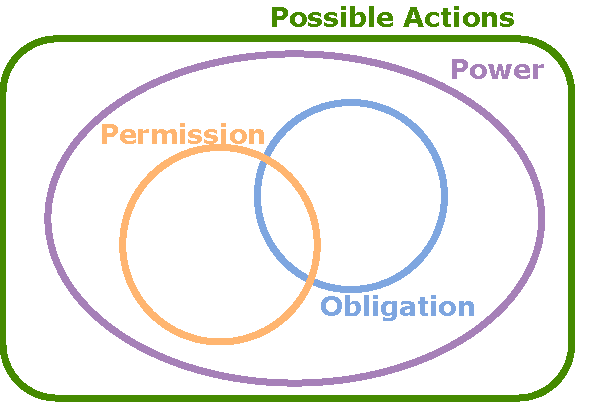
\includegraphics[width=0.6\textwidth]{05_iigo/images/SOMAS_per_obl.pdf}
\caption{Relationship between \emph{power}, \emph{permission} and \emph{obligation}.}
\label{fig:per_obl_sets}
\end{figure} 


For example, the Judge has the \emph{power} to carry out investigations at an IIGO session. There are no rules specifying which specific islands the Judge should investigate. Therefore, the Judge has the \emph{permission} to investigate any `alive' islands during a session. However, the Judge is \emph{obliged} to make at least some number of investigations each turn.



\section{Executive Branch}
\label{sec:executive}
The executive branch is responsible for \textbf{carrying out the law}.
\begin{itemize}
       
    \item The President has the \emph{power} to: 
    \begin{itemize}
        
        \item Select a rule for voting $R^{*}$ to be passed to the Speaker.
        \begin{rule_IIGO}
            The President has the \emph{obligation} to \emph{select} a rule $R^{*}$ if the \emph{rule proposal list} has at least one proposed rule in it.
        \end{rule_IIGO}
        \begin{rule_IIGO}
            The President has the \emph{permission} to \emph{select} a rule $R^{*}$ if and only if $R^{*} \in S$, where $S$ is the \emph{rule proposal list}.
        \end{rule_IIGO}
        
        \item Decide the amount of individual \emph{taxation} (i.e. a specific \emph{minimum} amount of contribution to the common pool for each island) for the current turn.
        
        \begin{itemize}
            \item The President is given the self-reported resource amounts held by each island to assist in this decision.
            %\item Suggested Rule: For any island that has chosen to not report it's resources, the President has the \emph{obligation} to set them an individual tax amount T.
        \end{itemize}
        
        \item Decide the allocation of resources distributed from the common pool to the islands (i.e. a specific \emph{maximum} amount an island is permitted to take from the common pool).
        
        \begin{itemize}
            \item The President is given the \emph{allocation requests} made by each island.
            %\item \emph{}{Suggested Rule:} The President has an obligation to prioritise islands in critical condition.
        \end{itemize}
    \end{itemize}
\end{itemize}



\section{Legislative Branch}
\label{sec:legislative}
The legislative branch is responsible for \textbf{making the law}.
\begin{itemize}

    \item The Speaker has the \emph{power} to:
    \begin{itemize}
        
        \item Call a vote $V$ for a rule $R$.
        \begin{rule_IIGO}
            The Speaker has the \emph{obligation} to \emph{call} a vote $V$ if and only if the President has \emph{selected} a rule $R$ to be voted on.
        \end {rule_IIGO}
        \begin{rule_IIGO}
            The Speaker has the \emph{permission} to \emph{call} a vote $V$ for a rule $R$ if and only if the rule $R = R^{*}$, where $R^{*}$ is the rule \emph{selected} by the President.
        \end {rule_IIGO}
            
        \item Choose which islands are participating in the vote $V$.
       % \footnote{This is our sequential implementation alternative for the power to close the ballot box.}.
        \begin{rule_IIGO}
            The Speaker has the \emph{obligation} to ask for a vote from all alive islands.
        \end {rule_IIGO}
            
        \item Declare the result $C$ of a vote $V$. 
        \begin{rule_IIGO}
            The Speaker has the \emph{obligation} to \emph{declare the result} $C$ for a vote $V$ if and only if the vote V has been \emph{called}.
        \end {rule_IIGO}
        \begin{rule_IIGO}
            The Speaker has the \emph{permission} to \emph{declare the result} $C$ for a vote $V$ if $C = C^{*}$, where $C^{*}$ is the result produced by \emph{calling} the vote $V$.
        \end {rule_IIGO}
        \begin{itemize}
            \item This step is what enables a rule to be \emph{active}.
        \end{itemize}
    \end{itemize}
\end{itemize}




\section{Judicial Branch}
\label{sec:judicial}

The judicial branch is responsible for \textbf{evaluating the law}.
\begin{itemize}
    \item The Judge has the \emph{power} to:
    \begin{itemize}
        \item Perform a number of \emph{inspections}\footnote{An \emph{inspection} \textbf{costs} an expense of resources (See Definition~\ref{def:invst} for more detail).} $I$ and produce a compliance outcome $\mathbb{O}^{*}$\footnote{Note that the compliance outcome $\mathbb{O}^{*}$ considered is a boolean.}.
        %(true: the island has been compliant with the rules in play, false: the island has not been compliant with the rules in play)
        %\begin{itemize}
           % \item For example, to check if the event outcome is \emph{concurrent}\footnote{Again, what is defined as "concurrent"? A clear definition is needed.} with the rules.
        %\end{itemize}
        \begin{rule_IIGO}
            The Judge has the \emph{obligation} to make at least $N$ investigations at each turn.
        \end{rule_IIGO}
        \item Declare the outcome $\mathbb{O}$ of an inspection $I$ to all islands\footnote{This act of broadcasting is especially important for islands to form an opinion about the sanctioned islands accordingly.}.
        \begin{rule_IIGO}
            The Judge has the \emph{obligation} to declare the outcome $\mathbb{O}$ of an inspection $I$ if and only if the inspection $I$ has been performed.
        \end{rule_IIGO}
        \begin{rule_IIGO}
            The Judge has the \emph{permission} to declare the outcome $\mathbb{O}$ of an inspection $I$ if $\mathbb{O} = \mathbb{O}^{*}$, where $\mathbb{O}^{*}$ is the outcome of the inspection $I$.
        \end{rule_IIGO}
        %\item Initiate the removal of the \texttt{President}.
        %\begin{itemize}
            %\item A good Judge would be especially vigilant during \emph{power transfer} regarding the \emph{President} position (see Section~\ref{leg_const} for more detail).
        %\end{itemize}
        \item Invoke economic \textbf{sanctions} (see Section~\ref{sec:sanctions} for more detail).
        \begin{rule_IIGO}
            The Judge has the \emph{obligation} to invoke a sanction $S$ for an island $X$ if and only if an investigation $I$ has an outcome $\mathbb{O}^{*}$ indicating non-compliance, and $I$ is an investigation of an action taken by island $X$.
        \end{rule_IIGO}
        \item Invoke even more severe sanctions in the case of further disobedience to previous sanction(s).
        \begin{rule_IIGO}
            The Judge has the \emph{permission} to invoke a severer sanction $S'$ for an island $X$ if the island $X$ has not fulfilled the requirements of the previous sanction $S$.
        \end{rule_IIGO}
        \item Pardon the islands which are currently sanctioned.
        \begin{rule_IIGO}
            The Judge has the \emph{permission} to revoke any sanction $S$ of an island $X$ at a specific turn.
        \end{rule_IIGO}
    \end{itemize}
\end{itemize}
%(e.g. a new rule that falls under a "sanction" category \hl{[I'm not sure about this being a `new rule` [Ezgi]]}

\subsection{Sanctions}
\label{sec:sanctions}
All sanctions are of economic nature which include:
        \begin{itemize}
            %\item Revoking an island's access to the common pool.
            \item Enforcing an island to contribute a specific amount of resources to the common pool.
            \begin{itemize}
                \item This does not mean that the Judge has the \emph{power} to take resources from an island in order to put them to the common pool -- the island itself is expected to carry out this implication imposed by the sanction itself, otherwise further punishment can be induced by the Judge.
                \item Similarly, \emph{opinion formulation} will follow accordingly whether the island(s) is/are following the implications imposed by the sanction(s).
            \end{itemize}
        
    \end{itemize}
    Sanctions are the associated penalty that comes with an island breaking a specific rule. The Judge is in full control of the penalties associated with breaking any rules. Once the Judge has specified the score of the penalty associated with each time an island breaks a rule, the cumulative penalties accumulated by the island are then used to determine which \textbf{sanction tier} that each island falls into. The score threshold to determine the boundaries of the sanction tiers are set by the Judge. At each turn of the game, each island is told whether they are being sanctioned, and if so, which \textbf{sanction tier} that they are currently in. The \textbf{sanction tiers} of the non-compliant islands are also broadcasted to the other islands in the archipelago. To summarise, the sanctioning process follows these steps:
    
    
    
    %Sanctions are based on an island breaking a rule. Each rule must therefore have an associated penalty. By default, we set these penalties such that they add $1$ to the total sanction score for each island. However, we allow the judge to override this scoring, the judge is able to set their own scores for any particular rule as they desire. This custom scoring is then used when an island breaks a particular rule. By looking at events that occurred in the last turn, and using the customised scoring we provide the holder of the judge role with full control of the penalties for breaking any rules.
    
    





%we then use the cumulative penalties accumulated by each island to determine which Sanction Tier they fall into. The score threshold's required to fall into these sanction tiers is set by the judge and is checked for monotonicity. Each island is told whether they are being sanctioned, and is so what tier they are in. We also tell other islands about which sanction tiers other islands have fallen into. 

    \begin{enumerate}
        \item The Judge has the \emph{power} to set custom penalties associated with breaking any rules.
        \item The Judge is given a list of all events that occurred in the previous turn.
        \item The Judge has the \emph{power} to check whether any, or all of these previous events, involve the islands in the archipelago breaking any rules.
        \item Each of the transgressions is scored using the Judge's custom penalties if the Judge has set them. Otherwise, a score of $1$ is given each time a rule is broken.
        \item The Judge has the \emph{power} to revise the sanction thresholds.
        \item Using the latest sanction thresholds available, each island is assigned to a sanction tier based on the sanction score that it has received.
        \item These sanction tiers are broadcasted to all of the islands in the archipelago.
        \item The Judge then uses sanctions rules in place to calculate the specific amount of resources that each non-compliant island has in order to determine how much it should contribute to the common pool, based on the sanction tier that it is in.
    \end{enumerate}



\section{Constitutional Rights and Obligations in the Archipelago}
\label{sec:const_rights_obl_archi}
Each island has the \emph{power} to:
\begin{itemize}
\item make an \emph{allocation request} (see Definition~\ref{def:alloc_req}) to the President for a specific amount to be allocated to them.
\item report the number of resources it is in possession of to the President.
\begin{rule_IIGO}
    Each island has the \emph{obligation} to report the number of resources it is in possession of to the President.
\end{rule_IIGO}
\begin{rule_IIGO}
    Each island has the \emph{permission} to report the number of resources $R'$ if and only if $R' = R$, where R is the number of resources the island is in possession of.
\end{rule_IIGO}
\item take resources from the common pool.


\begin{rule_IIGO}
    Each island has the \emph{permission} to take at maximum $N$ resources, where $N$ is the specific allocation made by the President to that island\footnote{If no such allocation is made, the island is \emph{permitted} to take any amount of resources.}.
\end{rule_IIGO}
\item contribute resources to the common pool.
\begin{rule_IIGO}
    Each island has the \emph{obligation} to contribute to the common pool an amount greater or equal to that of the individual tax set by the President.
\end{rule_IIGO}
                %The President is in
                %(unless there is a rule in place that dictates how Speaker is to allocate resources).
\item add a rule to the \emph{rule proposal list} (see Definition~\ref{def:rule_prop_list}) at the start of each turn.
        %\begin{itemize}
            %\item The game specification includes how many rules an island can propose each turn.
        %\end{itemize}
        %\item vote  for rules in the Legislative Branch and vote for their favourite islands in elections
\item participate in the legislative branch of the government by casting ballots in votes called by the Speaker
\item vote for an island to be elected for a specific role (e.g. the President, Judge, Speaker) during the elections\footnote{This will be assumed to be true \underline{unless stated otherwise}. %Note that \textbf{diplomatic sanctions} can disable this power of a specific island (see Section~\ref{jud_const}).}.
        }.
\end{itemize}
\section{Accountability Cycle}
\label{sec:accountability}


To ensure that the government avoids corruption and abuse of power, each branch is accountable to another. The President is accountable to the Speaker, the Speaker is accountable to the Judge, and the Judge is accountable to the President (see Figure~ \ref{fig:cycles_in_IIGO}). This accountability cycle is enacted through \emph{monitoring} actions\footnote{Note that the terms \textbf{monitoring} and \textbf{investigation} have similar but quite different meanings in the IIGO context.}. 

The powers related to the accountability cycle and transfer-of-power for each role can be summarized as the following: 
\begin{itemize}
    \item The Speaker has the \emph{power} to: 
    \begin{itemize}
        \item monitor the President.
        \item announce the result of this monitoring.
        \item initiate the transfer-of-power for the Judge.
    \end{itemize}
    \item The President has the \emph{power} to: 
    \begin{itemize}
        \item monitor the Judge.
        \item announce the result of this monitoring.
        \item initiate the transfer-of-power for the Speaker.
    \end{itemize}
    \item The Judge has the \emph{power} to: 
    \begin{itemize}
        \item  monitor the Speaker.
        \item announce the result of this monitoring.
        \item initiate the transfer-of-power for the President.
    \end{itemize}
\end{itemize}

%Unlike investigations performed by the Judge, who performs investigations on island actions in the following turn, each role is given the opportunity to check up on the actions of the role it is responsible for immediately after they have been performed. In this sense, the President can monitor (includes investigative-monitoring) the powers (calling a vote and announcing the result) acted on by the Speaker immediately after the Speaker's announcement (or lack there of). The government officials hold a lot of power so this is to ensure that any wrong-doing is determined as quickly as possible. For this project we are only pursuing one degree of monitoring, that is, the powers relating to the accountability cycle will not be monitored themselves. We assume that agents will act in the interest of themselves and keeping all the islands alive is beneficial to everyone. Hence, while the agents might be inclined to break rules in order to benefit themselves, anyone else breaking the rules is seen as undesirable under the assumption that the system in place is there to benefit all. 


Through the proposed accountability cycle, each role is given the opportunity to check up on the actions of the role it is accountable for immediately after they have been performed. It is clear that the IIGO roles (i.e. the President, Speaker and Judge) hold a considerable amount of \emph{power} in their hands. The accountability cycle is designed to address the possible abuses of this power. With monitoring, any wrong-doing in the IGO is determined as quickly as possible and the role in question can be replaced. 

Within the scope of the coursework, we decided to pursue only \emph{one degree of monitoring}, meaning that the powers relating to the accountability cycle will not be monitored themselves. We assume that agents will act in the interest of all the islands in the archipelago. Hence, while the agents might be inclined to break the rules to benefit in some form, it is assumed that the others will negatively see any non-compliant islands based on the assumption that the proposed IIGO system is in place to maintain the welfare of all the islands.

Let role $X$ be accountable to the role $Y$, which is accountable to the role $Z$. Then:
\begin{rule_IIGO}
$Y$ has the \emph{obligation} to declare the outcome of the monitoring result $M$ associated with the action $A$ undertaken by $X$ if and only if $Y$ has monitored the action $A$ performed by $X$. 
\end{rule_IIGO}
\begin{rule_IIGO}
$Y$ has the \emph{permission} to declare the monitoring result $M$ associated with the action $A$ undertaken by $X$ if and only if $M = M^{*}$, where $M^{*}$ is the outcome of \emph{monitoring} action $A$ performed by $X$\footnote{These constitutional rules should be available to the agents to check their decision against. However, due to having only one degree of accountability cycle in place, these rules are not enforced through any sanctions (i.e. breaking these rules has no consequences as they only deem to be an \emph{agreement} among the roles).}.
\end{rule_IIGO}


\begin{figure}[!htb]
\centering
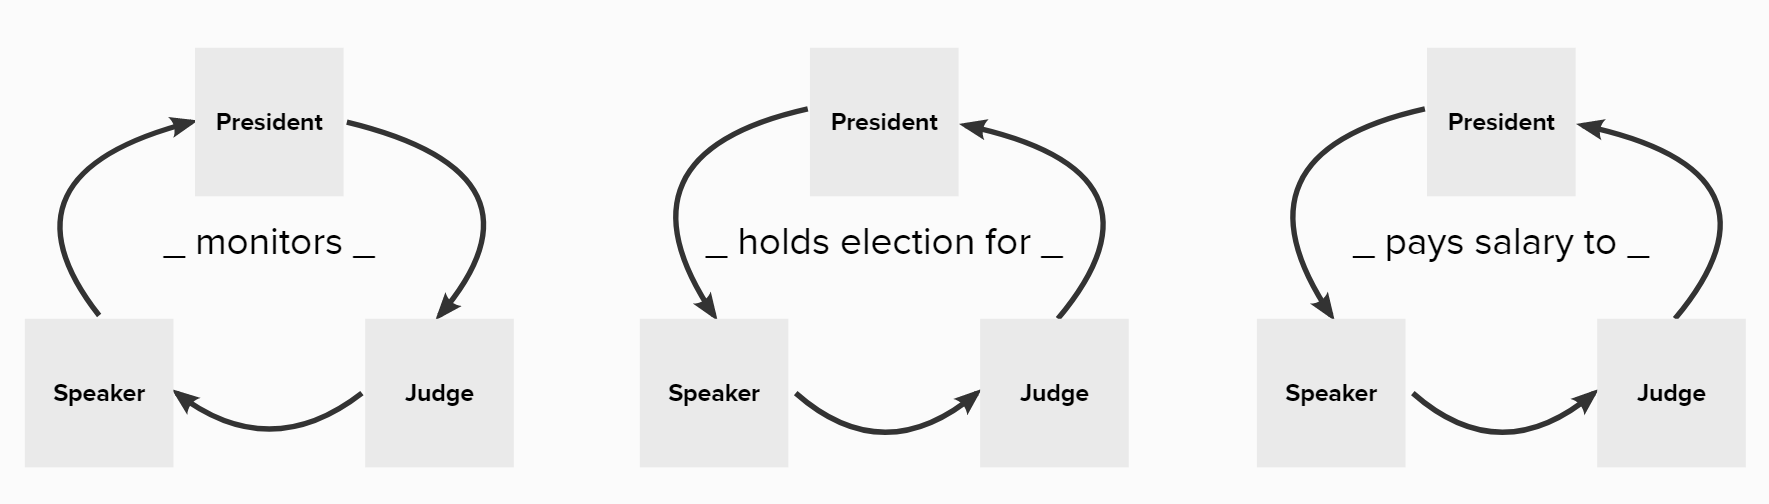
\includegraphics[scale=0.33]{05_iigo/images/role cycles.png}
\caption{Accountability cycle (left), the transfer-of-power cycle (middle) and salary cycle (right).}
\label{fig:cycles_in_IIGO}
\end{figure}


\subsection{Transfer-of-power}
\label{subsec:transfer-of-power}
\begin{enumerate}
    \item The Speaker conducts a vote for the election of the new Judge.
    \item The Judge conducts a vote for the election of the new President.
    \item The President conducts a vote for the election of the new Speaker.
\end{enumerate}
Refer to the Figure~ \ref{fig:cycles_in_IIGO} for further clarification about the transfer-of-power cycle.

\begin{rule_IIGO}
   The role $X$ has the \emph{obligation} to conduct a vote for the election of $Y$ at the end of the term (see Definition~\ref{def:term}) if and only if the role $X$ is accountable to the role $Y$. 
\end{rule_IIGO}.

\section{Budget and Salary}
\subsection{Budget}
%Actions associated with the IIGO have an associated cost that is defined as a configuration parameter. The institutional-power-enabled actions of  identified to require a "computational" component are:

Institutional-enabled-power actions in the IIGO have an associated cost with them. Some examples for such actions include:


%that is defined as a configuration parameter. The institutional-power-enabled actions of  identified to require a "computational" component are:


%We have defined the resource to be an endogenous one, hence any computation surrounding the distribution of the resource must use up some of that resource. 
\begin{itemize}
\item Calling any vote and computing the winner.
\item Declaring (e.g. \textit{announcing} the result of a vote).
\item Setting the amount of \emph{taxation} for each island.
\item Deciding the allocation distribution for each island.
\item Inspecting an island's action history.
\item Monitoring a role.
\end{itemize}

Since IIGO has been designed to act in the common good, IIGO-related costs will be directly withdrawn from the common pool. Since the common pool is considered a communal property of the archipelago, there are rules in place to limit how much each role is allowed to spend in order to perform its own institutional-power-enabled actions. This is the reason why defining the \emph{budget} and keeping it separate for each of the three IIGO roles.


As a role performs institutional-enabled-power actions, the corresponding cost associated with this action is subtracted from the role's budget. A budget of zero means that the role does not have the \emph{power} to perform any of its institutional-power-enabled actions. The removal of the budget rule from the rules in play means the role is allowed to perform as many such actions as it prefers to (as long as those actions are not governed by other rules). 



%As a role performs an endogenous-cost action, the corresponding cost associated with this action is subtracted from the role's budget. Thus, if as a result of an endogenous-cost action a role will be left with negative budget, it will have gone over the budget limit and will have broken the budget rule. A budget of zero means that the role is not allowed to perform any of its institutional-power-enabled actions associated an endogenous-cost. The removal of the budget rule from the rules in play means the role is allowed to perform as many such actions as it pleases (as long as those actions are not governed by other rules). 

The budget rule is also persistent across turns. This means that, assuming nothing else affects the budget, if a role has $100$ resources in its budget at each turn and spends only $10$ resources, this means that this very same role has $90$ resources in its budget at the next turn. On the other hand, islands can choose to increase the budget periodically every turn. This is governed by another budget extension rule.




%one turn and it spends 10, it has 90 resources in it's budget the next turn. 

Finally, it must be noted that the budget is inherently linked with the fact that whether obligations of a specific role can be undergone.
For example, during \emph{monitoring}, it should not be seen as a rule violation if a role has not acted on an obligation if it would go over the budget as a result. 

%This can also be seen as an added clause "... and the action is only permitted if they have the budget" to most rules which govern actions with an endogenous-cost.
%\begin{rule_IIGO}
    %The budget is increased by an amount $N$ every turn.
%\end{rule_IIGO}

%This rule means that, assuming nothing else affects the budget, if a budget is set to increase by 10 resources every turn and the budget is a 100 resources in turn one, the budget is 110 resources in turn 2. Setting this rule to 0 is equal to removing this rule and it means that the budget is never increased. 


\subsection{Salary}
\label{subsec:salary}
A salary is paid to each role in power as an incentive to act in a publicly approved way. %Hence, each role has the \emph{power} to pay a salary to another role following the salary cycle in Figure~\ref{fig:cycles_in_IIGO}.
\begin{rule_IIGO} \label{rule:salary}
   %Each role has the \emph{obligation} to pay the salary of amount $S$ to another if and only if the amount paid $S'$ is equal to $S$.
   Each role has the \emph{obligation} to pay the salary of amount $S$ to one another following the salary cycle in Figure~\ref{fig:cycles_in_IIGO}.
\end{rule_IIGO}

In Rule~\ref{rule:salary}, setting $S=0$ (through changing the active rules in place) means that roles do not have the permission to pay any salary. Removing the Rule~\ref{rule:salary} means that the roles may freely choose the amount $S$ for the salary payments.

\section{IIGO Session order}

\begin{enumerate}
    \item The Judge has the \emph{power} to check the history of actions to confirm whether the previously punished island(s) has/have obeyed the previous round's sanctions, meaning whether they contributed to the common pool accordingly in case of economic sanctions.
    %\begin{itemize}
      %  \item \emph{Suggested Rule:} In case of disobeying sanctions, the Judge is \emph{obliged} and \emph{permitted} to increase the severity of sanctions with respect to specific islands.
   % \end{itemize}
    \item The Judge has the \emph{power} to carry out \emph{inspections} on the history of actions of any island $X$ to check whether:
        \begin{enumerate}
        \item the reported resources of $X$ in the previous round match the real value of resources $X$ had in its private pool for the previous turn.
        \item the island $X$ has retrieved the right amount of the resources from the common pool, based on the \emph{allocation request} evaluated by the previous President.
            \begin{itemize}
            \item An example: In the previous round, the President has decided that the island $X$ can take $Y$ amount of resources from the common pool. If the Judge finds out that the island $X$ has taken an amount of $Y'$ such that $Y' > Y$, the Judge has the \emph{power} to invoke sanctions on the island $X$.
            
            %the Judge is \emph{obliged} and \emph{permitted} to sanction island $X$.
            \end{itemize}
        \end{enumerate}
    \item The Judge has the \emph{power} to invoke sanctions based on the outcome of the inspections.
    \item The President has the \emph{power} to decide to carry out a \emph{monitoring} on:
        \begin{enumerate}
        \item the sanctions imposed by the Judge.
        \end{enumerate}
    \item The islands may report the resources in their private pools to the President.
    \item The President has the \emph{power} to let each island know about the amount of \emph{taxation} they have to pay.
    \item The island has the \emph{power} to make an \emph{allocation request} to the President.
    \item The President has the \emph{power} decide on an allocation of resources and let each island know about the amount of resource allocation they are permitted to take from the common pool.
    \item The island has the \emph{power} to pick and to propose a rule to be voted on to the President.
    \item The President has the \emph{power} to choose a rule to be voted on from the received rule proposals.
    \item The Speaker has the \emph{power} to decide to carry out a \emph{monitoring} on: 
        \begin{enumerate}
        \item the resource allocation decided by the President.
        \item the rule proposed by the President.
        \end{enumerate}
    \item The Speaker has the \emph{power} to call a vote.
        \begin{enumerate}
        \item The islands vote in support of, or against, the rule (aye or nay) anonymously.
        \end{enumerate}
    \item The Speaker has the \emph{power} to announce a result of a vote to the islands and carries out the law change, if required (e.g. deleting/rejecting a rule if there is a majority nay vote).
    \item The Judge has the \emph{power} to decide to carry out \emph{monitoring} on:
        \begin{enumerate}
        \item the vote called by the Speaker.
        \item the Speaker announcing the result.
    \end{enumerate}
    \item The roles pay salary for one another following the accountability cycle in Figure~ \ref{fig:cycles_in_IIGO}.

\end{enumerate}



\section{Future Work}

\begin{itemize}
    \item \textbf{Diplomatic sanctions}: Although having the potential of being a good alternative for severer sanctions discussed in  Section~\ref{sec:sanctions}, diplomatic sanctions are \emph{not} implemented within the scope of the coursework. \\
    Suggested diplomatic sanctions include:
        \begin{itemize}
            \item Revoking an island's eligibility to vote and to be elected for a position.
            \item Revoking an island's eligibility to propose a rule/motion.
        \end{itemize}
    \item \textbf{Immutable rules}: Within the scope of the coursework, a subset of rules could have been categorised as immutable. This means that to change such immutable rules, the islands first need to vote to change their status to be \emph{mutable}, and consequently, hold another vote to change these mutable rules.
    %\item \textbf{Adding rules to the proposal list: } 
\end{itemize}

    \chapter{Inter-Island Governmental Organisation (IIGO)}


The role of IIGO is to maintain, update, and revise the rules concerning provision to managing the long-term collective risk dilemma (ltCRD). 

\begin{itemize}
    \item There will be 3 distinct branches in the IIGO: the \textbf{legislative branch}, \textbf{executive branch} and \textbf{judicial branch}\footnote{This is, as no surprise, inspired by the separation of powers in Western democracies.}.
    \item Each role is put in power according to the  transfer-of-power rules (see Section~\ref{subsec:transfer-of-power} for more detail).
    \item The head of the legislative branch is the Speaker, the head of the executive branch is the President, and the head of judicial branch is the Judge.
    \begin{itemize}
        \item  The Speaker, President and Judge are selected, through a democratic election, from the islands in the archipelago\footnote{This naming is inspired by the roles in the US Government.}.
        \item The resources gathered by the archipelago are endogenous, hence acting on the institutional powers granted to the Speaker, President or Judge costs resources. 
        \item For their duty, the President, the Speaker and the Judge receive a salary for each of their turns in office (see Section~\ref{subsec:salary} for more detail).
        \item The limit of the powers of the President, Speaker and Judge are defined in this chapter (e.g. the Speaker can only call one vote per turn).
 
    \end{itemize}
\end{itemize}

\subsection{IIGO Specific Definitions}
\begin{definition} \label{def:ballot}
    A \textbf{ballot} is related to each island's \textbf{power} to support or disagree with the rule specified in the vote called by the President and to vote in favour or against an island for a specific role (i.e. the President, Speaker, Judge) at each round of the game.
\end{definition}


%\begin{definition} \label{def:vote}
    %A \textbf{vote} is related to a role's (i.e. the President, Speaker, Judge) \textbf{power} to call a vote for a specific rule or an election.
%\end{definition}


\begin{definition} \label{def:tax}
    The \textbf{taxation} is related to the President's \textbf{power} to request a specific \underline{\textbf{minimum}} amount of contribution from each island to the common pool at each round of the game. 
\end{definition}

\begin{definition} \label{def:alloc_req}
    An \textbf{allocation request} is related to each island's \textbf{power} to request a specific amount of resource allocation from the President at each round of the game.
\end{definition}


\begin{definition} \label{def:rule_prop_list}
A \textbf{rule proposal list} is related to each island's \textbf{power} to propose a specific rule to be passed to the President at each round of the game.
\end{definition}

\begin{definition} \label{def:invst}
    An \textbf{investigation} is related to the Judge's \textbf{power} to acquire information to make a decision, followed by a calculation of the expected results and checking whether some specific rules have been obeyed, exclusively for the actions carried out by the \textbf{islands}. 
\end{definition}


An example of an \emph{investigation}: The President has permitted the island $X$ to take the amount of $Y$ resources from the common pool. Upon \emph{investigation} carried out by the Judge, it is revealed that the amount of resources taken out from the common pool by the island $X$ is, in fact, $Y'$ such that $Y' \neq Y$.


\begin{definition}
\textbf{Monitoring} is a government official's \textbf{power} to perform event recognition and to check whether some specific rules have been obeyed.
\end{definition}

An example of \emph{monitoring}: The Speaker has performed only the following action: \emph{counted the votes and calculated the result} for a rule. Upon \emph{monitoring} carried out by the President, it is noticed that the Speaker has not made any \emph{announcement}. Hence, the Speaker has not followed their obligation to \emph{announce} the result of any vote held.

See Section~\ref{sec:accountability} for more information about which roles can monitor which ones.


\begin{definition}
\textbf{Investigative-monitoring} is a government official's \textbf{power} to acquire the information used in acting on a governmental power followed by calculation of the expected results and checking whether some specific rules have been obeyed, exclusively for the actions carried out by a government official they are responsible for.
\end{definition}

An example of \emph{investigative-monitoring}: The Speaker has performed the following actions: \emph{counted the votes and calculated the result $R$} for a vote $V$ and \emph{announced} the result $R'$ for the vote $V$. Upon \emph{investigative-monitoring} carried out by the President, it is noticed that $R' \neq R$. Hence, the Speaker has modified the announced result.


\begin{definition}
The \textbf{sanction} is related to the Judge's \emph{power} to punish non-compliant islands when their disobedience is confirmed through investigations at a specific turn.
\end{definition}


\begin{definition}
The (judicial) \textbf{pardon} is related to the Judge's \emph{power} to forgive a non-compliant island at a specific turn.
\end{definition}

\begin{definition}
The \textbf{budget} is the maximum amount of resources a role is permitted to spend from the common pool as it performs its own institutional-power-enabled actions at a specific turn.
\end{definition}


\begin{definition}
The \textbf{salary} is the amount of resources a role is to be given from the common pool as a reward for performing its institutional-power-enabled actions at a specific turn.
\end{definition}

\begin{definition} \label{def:term}
A \textbf{term} is the number of turns an island is \emph{permitted} to hold a role, and after which the responsible role (indicated in the transfer-of-power cycle in Figure~\ref{fig:cycles_in_IIGO}) is \emph{obliged} to initiate transfer-of-power.
\end{definition}

\subsection{\emph{Power}, \emph{Permission} and \emph{Obligation} Distinction}
In the rest of the specifications, we will be specifically using the following three terms to define the actions and responsibilities carried out by the Speaker, President, Judge (see Figure~ \ref{fig:per_obl_sets}):
\begin{itemize}
    \item Power
    \item Permission
    \item Obligation
\end{itemize}



\begin{figure}[H] 
\centering
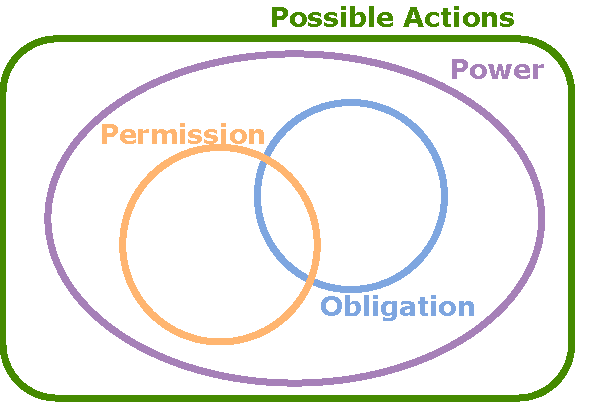
\includegraphics[width=0.6\textwidth]{05_iigo/images/SOMAS_per_obl.pdf}
\caption{Relationship between \emph{power}, \emph{permission} and \emph{obligation}.}
\label{fig:per_obl_sets}
\end{figure} 


For example, the Judge has the \emph{power} to carry out investigations at an IIGO session. There are no rules specifying which specific islands the Judge should investigate. Therefore, the Judge has the \emph{permission} to investigate any `alive' islands during a session. However, the Judge is \emph{obliged} to make at least some number of investigations each turn.



\section{Executive Branch}
\label{sec:executive}
The executive branch is responsible for \textbf{carrying out the law}.
\begin{itemize}
       
    \item The President has the \emph{power} to: 
    \begin{itemize}
        
        \item Select a rule for voting $R^{*}$ to be passed to the Speaker.
        \begin{rule_IIGO}
            The President has the \emph{obligation} to \emph{select} a rule $R^{*}$ if the \emph{rule proposal list} has at least one proposed rule in it.
        \end{rule_IIGO}
        \begin{rule_IIGO}
            The President has the \emph{permission} to \emph{select} a rule $R^{*}$ if and only if $R^{*} \in S$, where $S$ is the \emph{rule proposal list}.
        \end{rule_IIGO}
        
        \item Decide the amount of individual \emph{taxation} (i.e. a specific \emph{minimum} amount of contribution to the common pool for each island) for the current turn.
        
        \begin{itemize}
            \item The President is given the self-reported resource amounts held by each island to assist in this decision.
            %\item Suggested Rule: For any island that has chosen to not report it's resources, the President has the \emph{obligation} to set them an individual tax amount T.
        \end{itemize}
        
        \item Decide the allocation of resources distributed from the common pool to the islands (i.e. a specific \emph{maximum} amount an island is permitted to take from the common pool).
        
        \begin{itemize}
            \item The President is given the \emph{allocation requests} made by each island.
            %\item \emph{}{Suggested Rule:} The President has an obligation to prioritise islands in critical condition.
        \end{itemize}
    \end{itemize}
\end{itemize}



\section{Legislative Branch}
\label{sec:legislative}
The legislative branch is responsible for \textbf{making the law}.
\begin{itemize}

    \item The Speaker has the \emph{power} to:
    \begin{itemize}
        
        \item Call a vote $V$ for a rule $R$.
        \begin{rule_IIGO}
            The Speaker has the \emph{obligation} to \emph{call} a vote $V$ if and only if the President has \emph{selected} a rule $R$ to be voted on.
        \end {rule_IIGO}
        \begin{rule_IIGO}
            The Speaker has the \emph{permission} to \emph{call} a vote $V$ for a rule $R$ if and only if the rule $R = R^{*}$, where $R^{*}$ is the rule \emph{selected} by the President.
        \end {rule_IIGO}
            
        \item Choose which islands are participating in the vote $V$.
       % \footnote{This is our sequential implementation alternative for the power to close the ballot box.}.
        \begin{rule_IIGO}
            The Speaker has the \emph{obligation} to ask for a vote from all alive islands.
        \end {rule_IIGO}
            
        \item Declare the result $C$ of a vote $V$. 
        \begin{rule_IIGO}
            The Speaker has the \emph{obligation} to \emph{declare the result} $C$ for a vote $V$ if and only if the vote V has been \emph{called}.
        \end {rule_IIGO}
        \begin{rule_IIGO}
            The Speaker has the \emph{permission} to \emph{declare the result} $C$ for a vote $V$ if $C = C^{*}$, where $C^{*}$ is the result produced by \emph{calling} the vote $V$.
        \end {rule_IIGO}
        \begin{itemize}
            \item This step is what enables a rule to be \emph{active}.
        \end{itemize}
    \end{itemize}
\end{itemize}




\section{Judicial Branch}
\label{sec:judicial}

The judicial branch is responsible for \textbf{evaluating the law}.
\begin{itemize}
    \item The Judge has the \emph{power} to:
    \begin{itemize}
        \item Perform a number of \emph{inspections}\footnote{An \emph{inspection} \textbf{costs} an expense of resources (See Definition~\ref{def:invst} for more detail).} $I$ and produce a compliance outcome $\mathbb{O}^{*}$\footnote{Note that the compliance outcome $\mathbb{O}^{*}$ considered is a boolean.}.
        %(true: the island has been compliant with the rules in play, false: the island has not been compliant with the rules in play)
        %\begin{itemize}
           % \item For example, to check if the event outcome is \emph{concurrent}\footnote{Again, what is defined as "concurrent"? A clear definition is needed.} with the rules.
        %\end{itemize}
        \begin{rule_IIGO}
            The Judge has the \emph{obligation} to make at least $N$ investigations at each turn.
        \end{rule_IIGO}
        \item Declare the outcome $\mathbb{O}$ of an inspection $I$ to all islands\footnote{This act of broadcasting is especially important for islands to form an opinion about the sanctioned islands accordingly.}.
        \begin{rule_IIGO}
            The Judge has the \emph{obligation} to declare the outcome $\mathbb{O}$ of an inspection $I$ if and only if the inspection $I$ has been performed.
        \end{rule_IIGO}
        \begin{rule_IIGO}
            The Judge has the \emph{permission} to declare the outcome $\mathbb{O}$ of an inspection $I$ if $\mathbb{O} = \mathbb{O}^{*}$, where $\mathbb{O}^{*}$ is the outcome of the inspection $I$.
        \end{rule_IIGO}
        %\item Initiate the removal of the \texttt{President}.
        %\begin{itemize}
            %\item A good Judge would be especially vigilant during \emph{power transfer} regarding the \emph{President} position (see Section~\ref{leg_const} for more detail).
        %\end{itemize}
        \item Invoke economic \textbf{sanctions} (see Section~\ref{sec:sanctions} for more detail).
        \begin{rule_IIGO}
            The Judge has the \emph{obligation} to invoke a sanction $S$ for an island $X$ if and only if an investigation $I$ has an outcome $\mathbb{O}^{*}$ indicating non-compliance, and $I$ is an investigation of an action taken by island $X$.
        \end{rule_IIGO}
        \item Invoke even more severe sanctions in the case of further disobedience to previous sanction(s).
        \begin{rule_IIGO}
            The Judge has the \emph{permission} to invoke a severer sanction $S'$ for an island $X$ if the island $X$ has not fulfilled the requirements of the previous sanction $S$.
        \end{rule_IIGO}
        \item Pardon the islands which are currently sanctioned.
        \begin{rule_IIGO}
            The Judge has the \emph{permission} to revoke any sanction $S$ of an island $X$ at a specific turn.
        \end{rule_IIGO}
    \end{itemize}
\end{itemize}
%(e.g. a new rule that falls under a "sanction" category \hl{[I'm not sure about this being a `new rule` [Ezgi]]}

\subsection{Sanctions}
\label{sec:sanctions}
All sanctions are of economic nature which include:
        \begin{itemize}
            %\item Revoking an island's access to the common pool.
            \item Enforcing an island to contribute a specific amount of resources to the common pool.
            \begin{itemize}
                \item This does not mean that the Judge has the \emph{power} to take resources from an island in order to put them to the common pool -- the island itself is expected to carry out this implication imposed by the sanction itself, otherwise further punishment can be induced by the Judge.
                \item Similarly, \emph{opinion formulation} will follow accordingly whether the island(s) is/are following the implications imposed by the sanction(s).
            \end{itemize}
        
    \end{itemize}
    Sanctions are the associated penalty that comes with an island breaking a specific rule. The Judge is in full control of the penalties associated with breaking any rules. Once the Judge has specified the score of the penalty associated with each time an island breaks a rule, the cumulative penalties accumulated by the island are then used to determine which \textbf{sanction tier} that each island falls into. The score threshold to determine the boundaries of the sanction tiers are set by the Judge. At each turn of the game, each island is told whether they are being sanctioned, and if so, which \textbf{sanction tier} that they are currently in. The \textbf{sanction tiers} of the non-compliant islands are also broadcasted to the other islands in the archipelago. To summarise, the sanctioning process follows these steps:
    
    
    
    %Sanctions are based on an island breaking a rule. Each rule must therefore have an associated penalty. By default, we set these penalties such that they add $1$ to the total sanction score for each island. However, we allow the judge to override this scoring, the judge is able to set their own scores for any particular rule as they desire. This custom scoring is then used when an island breaks a particular rule. By looking at events that occurred in the last turn, and using the customised scoring we provide the holder of the judge role with full control of the penalties for breaking any rules.
    
    





%we then use the cumulative penalties accumulated by each island to determine which Sanction Tier they fall into. The score threshold's required to fall into these sanction tiers is set by the judge and is checked for monotonicity. Each island is told whether they are being sanctioned, and is so what tier they are in. We also tell other islands about which sanction tiers other islands have fallen into. 

    \begin{enumerate}
        \item The Judge has the \emph{power} to set custom penalties associated with breaking any rules.
        \item The Judge is given a list of all events that occurred in the previous turn.
        \item The Judge has the \emph{power} to check whether any, or all of these previous events, involve the islands in the archipelago breaking any rules.
        \item Each of the transgressions is scored using the Judge's custom penalties if the Judge has set them. Otherwise, a score of $1$ is given each time a rule is broken.
        \item The Judge has the \emph{power} to revise the sanction thresholds.
        \item Using the latest sanction thresholds available, each island is assigned to a sanction tier based on the sanction score that it has received.
        \item These sanction tiers are broadcasted to all of the islands in the archipelago.
        \item The Judge then uses sanctions rules in place to calculate the specific amount of resources that each non-compliant island has in order to determine how much it should contribute to the common pool, based on the sanction tier that it is in.
    \end{enumerate}



\section{Constitutional Rights and Obligations in the Archipelago}
\label{sec:const_rights_obl_archi}
Each island has the \emph{power} to:
\begin{itemize}
\item make an \emph{allocation request} (see Definition~\ref{def:alloc_req}) to the President for a specific amount to be allocated to them.
\item report the number of resources it is in possession of to the President.
\begin{rule_IIGO}
    Each island has the \emph{obligation} to report the number of resources it is in possession of to the President.
\end{rule_IIGO}
\begin{rule_IIGO}
    Each island has the \emph{permission} to report the number of resources $R'$ if and only if $R' = R$, where R is the number of resources the island is in possession of.
\end{rule_IIGO}
\item take resources from the common pool.


\begin{rule_IIGO}
    Each island has the \emph{permission} to take at maximum $N$ resources, where $N$ is the specific allocation made by the President to that island\footnote{If no such allocation is made, the island is \emph{permitted} to take any amount of resources.}.
\end{rule_IIGO}
\item contribute resources to the common pool.
\begin{rule_IIGO}
    Each island has the \emph{obligation} to contribute to the common pool an amount greater or equal to that of the individual tax set by the President.
\end{rule_IIGO}
                %The President is in
                %(unless there is a rule in place that dictates how Speaker is to allocate resources).
\item add a rule to the \emph{rule proposal list} (see Definition~\ref{def:rule_prop_list}) at the start of each turn.
        %\begin{itemize}
            %\item The game specification includes how many rules an island can propose each turn.
        %\end{itemize}
        %\item vote  for rules in the Legislative Branch and vote for their favourite islands in elections
\item participate in the legislative branch of the government by casting ballots in votes called by the Speaker
\item vote for an island to be elected for a specific role (e.g. the President, Judge, Speaker) during the elections\footnote{This will be assumed to be true \underline{unless stated otherwise}. %Note that \textbf{diplomatic sanctions} can disable this power of a specific island (see Section~\ref{jud_const}).}.
        }.
\end{itemize}
\section{Accountability Cycle}
\label{sec:accountability}


To ensure that the government avoids corruption and abuse of power, each branch is accountable to another. The President is accountable to the Speaker, the Speaker is accountable to the Judge, and the Judge is accountable to the President (see Figure~ \ref{fig:cycles_in_IIGO}). This accountability cycle is enacted through \emph{monitoring} actions\footnote{Note that the terms \textbf{monitoring} and \textbf{investigation} have similar but quite different meanings in the IIGO context.}. 

The powers related to the accountability cycle and transfer-of-power for each role can be summarized as the following: 
\begin{itemize}
    \item The Speaker has the \emph{power} to: 
    \begin{itemize}
        \item monitor the President.
        \item announce the result of this monitoring.
        \item initiate the transfer-of-power for the Judge.
    \end{itemize}
    \item The President has the \emph{power} to: 
    \begin{itemize}
        \item monitor the Judge.
        \item announce the result of this monitoring.
        \item initiate the transfer-of-power for the Speaker.
    \end{itemize}
    \item The Judge has the \emph{power} to: 
    \begin{itemize}
        \item  monitor the Speaker.
        \item announce the result of this monitoring.
        \item initiate the transfer-of-power for the President.
    \end{itemize}
\end{itemize}

%Unlike investigations performed by the Judge, who performs investigations on island actions in the following turn, each role is given the opportunity to check up on the actions of the role it is responsible for immediately after they have been performed. In this sense, the President can monitor (includes investigative-monitoring) the powers (calling a vote and announcing the result) acted on by the Speaker immediately after the Speaker's announcement (or lack there of). The government officials hold a lot of power so this is to ensure that any wrong-doing is determined as quickly as possible. For this project we are only pursuing one degree of monitoring, that is, the powers relating to the accountability cycle will not be monitored themselves. We assume that agents will act in the interest of themselves and keeping all the islands alive is beneficial to everyone. Hence, while the agents might be inclined to break rules in order to benefit themselves, anyone else breaking the rules is seen as undesirable under the assumption that the system in place is there to benefit all. 


Through the proposed accountability cycle, each role is given the opportunity to check up on the actions of the role it is accountable for immediately after they have been performed. It is clear that the IIGO roles (i.e. the President, Speaker and Judge) hold a considerable amount of \emph{power} in their hands. The accountability cycle is designed to address the possible abuses of this power. With monitoring, any wrong-doing in the IGO is determined as quickly as possible and the role in question can be replaced. 

Within the scope of the coursework, we decided to pursue only \emph{one degree of monitoring}, meaning that the powers relating to the accountability cycle will not be monitored themselves. We assume that agents will act in the interest of all the islands in the archipelago. Hence, while the agents might be inclined to break the rules to benefit in some form, it is assumed that the others will negatively see any non-compliant islands based on the assumption that the proposed IIGO system is in place to maintain the welfare of all the islands.

Let role $X$ be accountable to the role $Y$, which is accountable to the role $Z$. Then:
\begin{rule_IIGO}
$Y$ has the \emph{obligation} to declare the outcome of the monitoring result $M$ associated with the action $A$ undertaken by $X$ if and only if $Y$ has monitored the action $A$ performed by $X$. 
\end{rule_IIGO}
\begin{rule_IIGO}
$Y$ has the \emph{permission} to declare the monitoring result $M$ associated with the action $A$ undertaken by $X$ if and only if $M = M^{*}$, where $M^{*}$ is the outcome of \emph{monitoring} action $A$ performed by $X$\footnote{These constitutional rules should be available to the agents to check their decision against. However, due to having only one degree of accountability cycle in place, these rules are not enforced through any sanctions (i.e. breaking these rules has no consequences as they only deem to be an \emph{agreement} among the roles).}.
\end{rule_IIGO}


\begin{figure}[!htb]
\centering
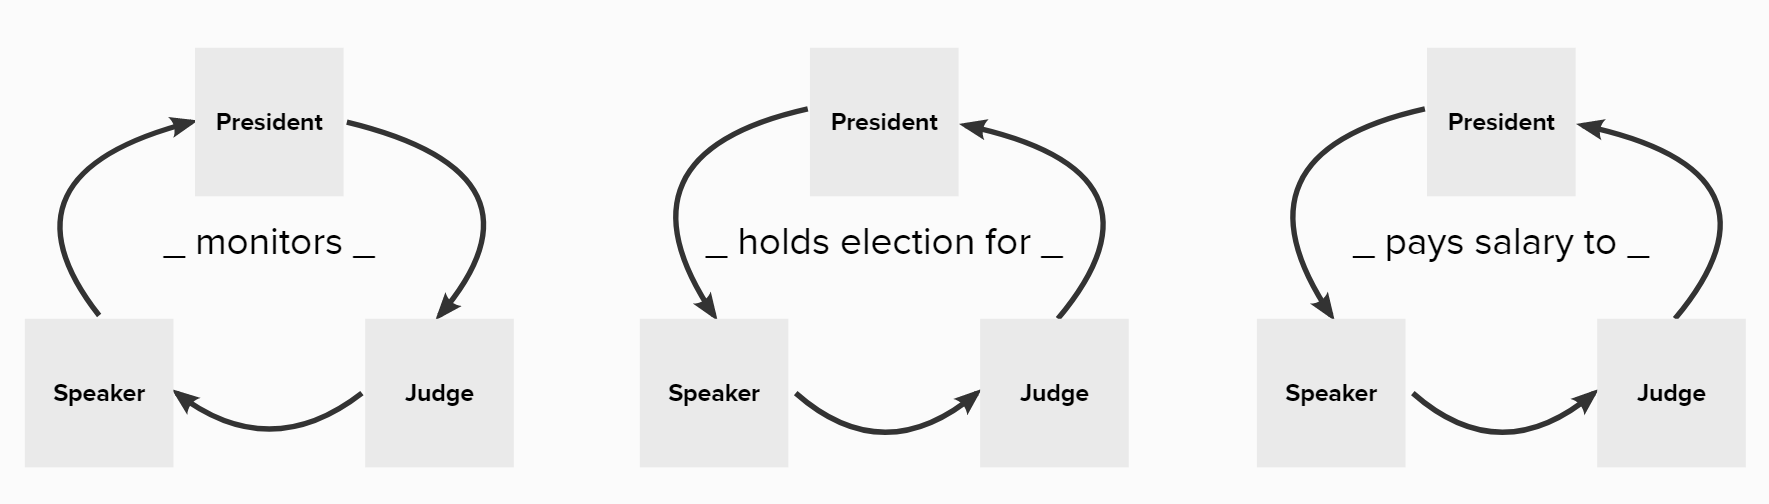
\includegraphics[scale=0.33]{05_iigo/images/role cycles.png}
\caption{Accountability cycle (left), the transfer-of-power cycle (middle) and salary cycle (right).}
\label{fig:cycles_in_IIGO}
\end{figure}


\subsection{Transfer-of-power}
\label{subsec:transfer-of-power}
\begin{enumerate}
    \item The Speaker conducts a vote for the election of the new Judge.
    \item The Judge conducts a vote for the election of the new President.
    \item The President conducts a vote for the election of the new Speaker.
\end{enumerate}
Refer to the Figure~ \ref{fig:cycles_in_IIGO} for further clarification about the transfer-of-power cycle.

\begin{rule_IIGO}
   The role $X$ has the \emph{obligation} to conduct a vote for the election of $Y$ at the end of the term (see Definition~\ref{def:term}) if and only if the role $X$ is accountable to the role $Y$. 
\end{rule_IIGO}.

\section{Budget and Salary}
\subsection{Budget}
%Actions associated with the IIGO have an associated cost that is defined as a configuration parameter. The institutional-power-enabled actions of  identified to require a "computational" component are:

Institutional-enabled-power actions in the IIGO have an associated cost with them. Some examples for such actions include:


%that is defined as a configuration parameter. The institutional-power-enabled actions of  identified to require a "computational" component are:


%We have defined the resource to be an endogenous one, hence any computation surrounding the distribution of the resource must use up some of that resource. 
\begin{itemize}
\item Calling any vote and computing the winner.
\item Declaring (e.g. \textit{announcing} the result of a vote).
\item Setting the amount of \emph{taxation} for each island.
\item Deciding the allocation distribution for each island.
\item Inspecting an island's action history.
\item Monitoring a role.
\end{itemize}

Since IIGO has been designed to act in the common good, IIGO-related costs will be directly withdrawn from the common pool. Since the common pool is considered a communal property of the archipelago, there are rules in place to limit how much each role is allowed to spend in order to perform its own institutional-power-enabled actions. This is the reason why defining the \emph{budget} and keeping it separate for each of the three IIGO roles.


As a role performs institutional-enabled-power actions, the corresponding cost associated with this action is subtracted from the role's budget. A budget of zero means that the role does not have the \emph{power} to perform any of its institutional-power-enabled actions. The removal of the budget rule from the rules in play means the role is allowed to perform as many such actions as it prefers to (as long as those actions are not governed by other rules). 



%As a role performs an endogenous-cost action, the corresponding cost associated with this action is subtracted from the role's budget. Thus, if as a result of an endogenous-cost action a role will be left with negative budget, it will have gone over the budget limit and will have broken the budget rule. A budget of zero means that the role is not allowed to perform any of its institutional-power-enabled actions associated an endogenous-cost. The removal of the budget rule from the rules in play means the role is allowed to perform as many such actions as it pleases (as long as those actions are not governed by other rules). 

The budget rule is also persistent across turns. This means that, assuming nothing else affects the budget, if a role has $100$ resources in its budget at each turn and spends only $10$ resources, this means that this very same role has $90$ resources in its budget at the next turn. On the other hand, islands can choose to increase the budget periodically every turn. This is governed by another budget extension rule.




%one turn and it spends 10, it has 90 resources in it's budget the next turn. 

Finally, it must be noted that the budget is inherently linked with the fact that whether obligations of a specific role can be undergone.
For example, during \emph{monitoring}, it should not be seen as a rule violation if a role has not acted on an obligation if it would go over the budget as a result. 

%This can also be seen as an added clause "... and the action is only permitted if they have the budget" to most rules which govern actions with an endogenous-cost.
%\begin{rule_IIGO}
    %The budget is increased by an amount $N$ every turn.
%\end{rule_IIGO}

%This rule means that, assuming nothing else affects the budget, if a budget is set to increase by 10 resources every turn and the budget is a 100 resources in turn one, the budget is 110 resources in turn 2. Setting this rule to 0 is equal to removing this rule and it means that the budget is never increased. 


\subsection{Salary}
\label{subsec:salary}
A salary is paid to each role in power as an incentive to act in a publicly approved way. %Hence, each role has the \emph{power} to pay a salary to another role following the salary cycle in Figure~\ref{fig:cycles_in_IIGO}.
\begin{rule_IIGO} \label{rule:salary}
   %Each role has the \emph{obligation} to pay the salary of amount $S$ to another if and only if the amount paid $S'$ is equal to $S$.
   Each role has the \emph{obligation} to pay the salary of amount $S$ to one another following the salary cycle in Figure~\ref{fig:cycles_in_IIGO}.
\end{rule_IIGO}

In Rule~\ref{rule:salary}, setting $S=0$ (through changing the active rules in place) means that roles do not have the permission to pay any salary. Removing the Rule~\ref{rule:salary} means that the roles may freely choose the amount $S$ for the salary payments.

\section{IIGO Session order}

\begin{enumerate}
    \item The Judge has the \emph{power} to check the history of actions to confirm whether the previously punished island(s) has/have obeyed the previous round's sanctions, meaning whether they contributed to the common pool accordingly in case of economic sanctions.
    %\begin{itemize}
      %  \item \emph{Suggested Rule:} In case of disobeying sanctions, the Judge is \emph{obliged} and \emph{permitted} to increase the severity of sanctions with respect to specific islands.
   % \end{itemize}
    \item The Judge has the \emph{power} to carry out \emph{inspections} on the history of actions of any island $X$ to check whether:
        \begin{enumerate}
        \item the reported resources of $X$ in the previous round match the real value of resources $X$ had in its private pool for the previous turn.
        \item the island $X$ has retrieved the right amount of the resources from the common pool, based on the \emph{allocation request} evaluated by the previous President.
            \begin{itemize}
            \item An example: In the previous round, the President has decided that the island $X$ can take $Y$ amount of resources from the common pool. If the Judge finds out that the island $X$ has taken an amount of $Y'$ such that $Y' > Y$, the Judge has the \emph{power} to invoke sanctions on the island $X$.
            
            %the Judge is \emph{obliged} and \emph{permitted} to sanction island $X$.
            \end{itemize}
        \end{enumerate}
    \item The Judge has the \emph{power} to invoke sanctions based on the outcome of the inspections.
    \item The President has the \emph{power} to decide to carry out a \emph{monitoring} on:
        \begin{enumerate}
        \item the sanctions imposed by the Judge.
        \end{enumerate}
    \item The islands may report the resources in their private pools to the President.
    \item The President has the \emph{power} to let each island know about the amount of \emph{taxation} they have to pay.
    \item The island has the \emph{power} to make an \emph{allocation request} to the President.
    \item The President has the \emph{power} decide on an allocation of resources and let each island know about the amount of resource allocation they are permitted to take from the common pool.
    \item The island has the \emph{power} to pick and to propose a rule to be voted on to the President.
    \item The President has the \emph{power} to choose a rule to be voted on from the received rule proposals.
    \item The Speaker has the \emph{power} to decide to carry out a \emph{monitoring} on: 
        \begin{enumerate}
        \item the resource allocation decided by the President.
        \item the rule proposed by the President.
        \end{enumerate}
    \item The Speaker has the \emph{power} to call a vote.
        \begin{enumerate}
        \item The islands vote in support of, or against, the rule (aye or nay) anonymously.
        \end{enumerate}
    \item The Speaker has the \emph{power} to announce a result of a vote to the islands and carries out the law change, if required (e.g. deleting/rejecting a rule if there is a majority nay vote).
    \item The Judge has the \emph{power} to decide to carry out \emph{monitoring} on:
        \begin{enumerate}
        \item the vote called by the Speaker.
        \item the Speaker announcing the result.
    \end{enumerate}
    \item The roles pay salary for one another following the accountability cycle in Figure~ \ref{fig:cycles_in_IIGO}.

\end{enumerate}



\section{Future Work}

\begin{itemize}
    \item \textbf{Diplomatic sanctions}: Although having the potential of being a good alternative for severer sanctions discussed in  Section~\ref{sec:sanctions}, diplomatic sanctions are \emph{not} implemented within the scope of the coursework. \\
    Suggested diplomatic sanctions include:
        \begin{itemize}
            \item Revoking an island's eligibility to vote and to be elected for a position.
            \item Revoking an island's eligibility to propose a rule/motion.
        \end{itemize}
    \item \textbf{Immutable rules}: Within the scope of the coursework, a subset of rules could have been categorised as immutable. This means that to change such immutable rules, the islands first need to vote to change their status to be \emph{mutable}, and consequently, hold another vote to change these mutable rules.
    %\item \textbf{Adding rules to the proposal list: } 
\end{itemize}

    \chapter{Inter-Island Governmental Organisation (IIGO)}


The role of IIGO is to maintain, update, and revise the rules concerning provision to managing the long-term collective risk dilemma (ltCRD). 

\begin{itemize}
    \item There will be 3 distinct branches in the IIGO: the \textbf{legislative branch}, \textbf{executive branch} and \textbf{judicial branch}\footnote{This is, as no surprise, inspired by the separation of powers in Western democracies.}.
    \item Each role is put in power according to the  transfer-of-power rules (see Section~\ref{subsec:transfer-of-power} for more detail).
    \item The head of the legislative branch is the Speaker, the head of the executive branch is the President, and the head of judicial branch is the Judge.
    \begin{itemize}
        \item  The Speaker, President and Judge are selected, through a democratic election, from the islands in the archipelago\footnote{This naming is inspired by the roles in the US Government.}.
        \item The resources gathered by the archipelago are endogenous, hence acting on the institutional powers granted to the Speaker, President or Judge costs resources. 
        \item For their duty, the President, the Speaker and the Judge receive a salary for each of their turns in office (see Section~\ref{subsec:salary} for more detail).
        \item The limit of the powers of the President, Speaker and Judge are defined in this chapter (e.g. the Speaker can only call one vote per turn).
 
    \end{itemize}
\end{itemize}

\subsection{IIGO Specific Definitions}
\begin{definition} \label{def:ballot}
    A \textbf{ballot} is related to each island's \textbf{power} to support or disagree with the rule specified in the vote called by the President and to vote in favour or against an island for a specific role (i.e. the President, Speaker, Judge) at each round of the game.
\end{definition}


%\begin{definition} \label{def:vote}
    %A \textbf{vote} is related to a role's (i.e. the President, Speaker, Judge) \textbf{power} to call a vote for a specific rule or an election.
%\end{definition}


\begin{definition} \label{def:tax}
    The \textbf{taxation} is related to the President's \textbf{power} to request a specific \underline{\textbf{minimum}} amount of contribution from each island to the common pool at each round of the game. 
\end{definition}

\begin{definition} \label{def:alloc_req}
    An \textbf{allocation request} is related to each island's \textbf{power} to request a specific amount of resource allocation from the President at each round of the game.
\end{definition}


\begin{definition} \label{def:rule_prop_list}
A \textbf{rule proposal list} is related to each island's \textbf{power} to propose a specific rule to be passed to the President at each round of the game.
\end{definition}

\begin{definition} \label{def:invst}
    An \textbf{investigation} is related to the Judge's \textbf{power} to acquire information to make a decision, followed by a calculation of the expected results and checking whether some specific rules have been obeyed, exclusively for the actions carried out by the \textbf{islands}. 
\end{definition}


An example of an \emph{investigation}: The President has permitted the island $X$ to take the amount of $Y$ resources from the common pool. Upon \emph{investigation} carried out by the Judge, it is revealed that the amount of resources taken out from the common pool by the island $X$ is, in fact, $Y'$ such that $Y' \neq Y$.


\begin{definition}
\textbf{Monitoring} is a government official's \textbf{power} to perform event recognition and to check whether some specific rules have been obeyed.
\end{definition}

An example of \emph{monitoring}: The Speaker has performed only the following action: \emph{counted the votes and calculated the result} for a rule. Upon \emph{monitoring} carried out by the President, it is noticed that the Speaker has not made any \emph{announcement}. Hence, the Speaker has not followed their obligation to \emph{announce} the result of any vote held.

See Section~\ref{sec:accountability} for more information about which roles can monitor which ones.


\begin{definition}
\textbf{Investigative-monitoring} is a government official's \textbf{power} to acquire the information used in acting on a governmental power followed by calculation of the expected results and checking whether some specific rules have been obeyed, exclusively for the actions carried out by a government official they are responsible for.
\end{definition}

An example of \emph{investigative-monitoring}: The Speaker has performed the following actions: \emph{counted the votes and calculated the result $R$} for a vote $V$ and \emph{announced} the result $R'$ for the vote $V$. Upon \emph{investigative-monitoring} carried out by the President, it is noticed that $R' \neq R$. Hence, the Speaker has modified the announced result.


\begin{definition}
The \textbf{sanction} is related to the Judge's \emph{power} to punish non-compliant islands when their disobedience is confirmed through investigations at a specific turn.
\end{definition}


\begin{definition}
The (judicial) \textbf{pardon} is related to the Judge's \emph{power} to forgive a non-compliant island at a specific turn.
\end{definition}

\begin{definition}
The \textbf{budget} is the maximum amount of resources a role is permitted to spend from the common pool as it performs its own institutional-power-enabled actions at a specific turn.
\end{definition}


\begin{definition}
The \textbf{salary} is the amount of resources a role is to be given from the common pool as a reward for performing its institutional-power-enabled actions at a specific turn.
\end{definition}

\begin{definition} \label{def:term}
A \textbf{term} is the number of turns an island is \emph{permitted} to hold a role, and after which the responsible role (indicated in the transfer-of-power cycle in Figure~\ref{fig:cycles_in_IIGO}) is \emph{obliged} to initiate transfer-of-power.
\end{definition}

\subsection{\emph{Power}, \emph{Permission} and \emph{Obligation} Distinction}
In the rest of the specifications, we will be specifically using the following three terms to define the actions and responsibilities carried out by the Speaker, President, Judge (see Figure~ \ref{fig:per_obl_sets}):
\begin{itemize}
    \item Power
    \item Permission
    \item Obligation
\end{itemize}



\begin{figure}[H] 
\centering
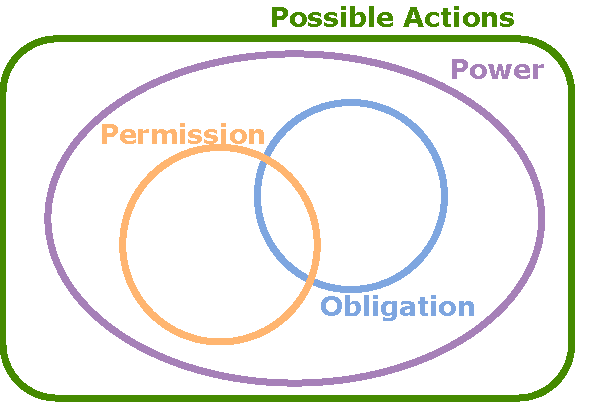
\includegraphics[width=0.6\textwidth]{05_iigo/images/SOMAS_per_obl.pdf}
\caption{Relationship between \emph{power}, \emph{permission} and \emph{obligation}.}
\label{fig:per_obl_sets}
\end{figure} 


For example, the Judge has the \emph{power} to carry out investigations at an IIGO session. There are no rules specifying which specific islands the Judge should investigate. Therefore, the Judge has the \emph{permission} to investigate any `alive' islands during a session. However, the Judge is \emph{obliged} to make at least some number of investigations each turn.



\section{Executive Branch}
\label{sec:executive}
The executive branch is responsible for \textbf{carrying out the law}.
\begin{itemize}
       
    \item The President has the \emph{power} to: 
    \begin{itemize}
        
        \item Select a rule for voting $R^{*}$ to be passed to the Speaker.
        \begin{rule_IIGO}
            The President has the \emph{obligation} to \emph{select} a rule $R^{*}$ if the \emph{rule proposal list} has at least one proposed rule in it.
        \end{rule_IIGO}
        \begin{rule_IIGO}
            The President has the \emph{permission} to \emph{select} a rule $R^{*}$ if and only if $R^{*} \in S$, where $S$ is the \emph{rule proposal list}.
        \end{rule_IIGO}
        
        \item Decide the amount of individual \emph{taxation} (i.e. a specific \emph{minimum} amount of contribution to the common pool for each island) for the current turn.
        
        \begin{itemize}
            \item The President is given the self-reported resource amounts held by each island to assist in this decision.
            %\item Suggested Rule: For any island that has chosen to not report it's resources, the President has the \emph{obligation} to set them an individual tax amount T.
        \end{itemize}
        
        \item Decide the allocation of resources distributed from the common pool to the islands (i.e. a specific \emph{maximum} amount an island is permitted to take from the common pool).
        
        \begin{itemize}
            \item The President is given the \emph{allocation requests} made by each island.
            %\item \emph{}{Suggested Rule:} The President has an obligation to prioritise islands in critical condition.
        \end{itemize}
    \end{itemize}
\end{itemize}



\section{Legislative Branch}
\label{sec:legislative}
The legislative branch is responsible for \textbf{making the law}.
\begin{itemize}

    \item The Speaker has the \emph{power} to:
    \begin{itemize}
        
        \item Call a vote $V$ for a rule $R$.
        \begin{rule_IIGO}
            The Speaker has the \emph{obligation} to \emph{call} a vote $V$ if and only if the President has \emph{selected} a rule $R$ to be voted on.
        \end {rule_IIGO}
        \begin{rule_IIGO}
            The Speaker has the \emph{permission} to \emph{call} a vote $V$ for a rule $R$ if and only if the rule $R = R^{*}$, where $R^{*}$ is the rule \emph{selected} by the President.
        \end {rule_IIGO}
            
        \item Choose which islands are participating in the vote $V$.
       % \footnote{This is our sequential implementation alternative for the power to close the ballot box.}.
        \begin{rule_IIGO}
            The Speaker has the \emph{obligation} to ask for a vote from all alive islands.
        \end {rule_IIGO}
            
        \item Declare the result $C$ of a vote $V$. 
        \begin{rule_IIGO}
            The Speaker has the \emph{obligation} to \emph{declare the result} $C$ for a vote $V$ if and only if the vote V has been \emph{called}.
        \end {rule_IIGO}
        \begin{rule_IIGO}
            The Speaker has the \emph{permission} to \emph{declare the result} $C$ for a vote $V$ if $C = C^{*}$, where $C^{*}$ is the result produced by \emph{calling} the vote $V$.
        \end {rule_IIGO}
        \begin{itemize}
            \item This step is what enables a rule to be \emph{active}.
        \end{itemize}
    \end{itemize}
\end{itemize}




\section{Judicial Branch}
\label{sec:judicial}

The judicial branch is responsible for \textbf{evaluating the law}.
\begin{itemize}
    \item The Judge has the \emph{power} to:
    \begin{itemize}
        \item Perform a number of \emph{inspections}\footnote{An \emph{inspection} \textbf{costs} an expense of resources (See Definition~\ref{def:invst} for more detail).} $I$ and produce a compliance outcome $\mathbb{O}^{*}$\footnote{Note that the compliance outcome $\mathbb{O}^{*}$ considered is a boolean.}.
        %(true: the island has been compliant with the rules in play, false: the island has not been compliant with the rules in play)
        %\begin{itemize}
           % \item For example, to check if the event outcome is \emph{concurrent}\footnote{Again, what is defined as "concurrent"? A clear definition is needed.} with the rules.
        %\end{itemize}
        \begin{rule_IIGO}
            The Judge has the \emph{obligation} to make at least $N$ investigations at each turn.
        \end{rule_IIGO}
        \item Declare the outcome $\mathbb{O}$ of an inspection $I$ to all islands\footnote{This act of broadcasting is especially important for islands to form an opinion about the sanctioned islands accordingly.}.
        \begin{rule_IIGO}
            The Judge has the \emph{obligation} to declare the outcome $\mathbb{O}$ of an inspection $I$ if and only if the inspection $I$ has been performed.
        \end{rule_IIGO}
        \begin{rule_IIGO}
            The Judge has the \emph{permission} to declare the outcome $\mathbb{O}$ of an inspection $I$ if $\mathbb{O} = \mathbb{O}^{*}$, where $\mathbb{O}^{*}$ is the outcome of the inspection $I$.
        \end{rule_IIGO}
        %\item Initiate the removal of the \texttt{President}.
        %\begin{itemize}
            %\item A good Judge would be especially vigilant during \emph{power transfer} regarding the \emph{President} position (see Section~\ref{leg_const} for more detail).
        %\end{itemize}
        \item Invoke economic \textbf{sanctions} (see Section~\ref{sec:sanctions} for more detail).
        \begin{rule_IIGO}
            The Judge has the \emph{obligation} to invoke a sanction $S$ for an island $X$ if and only if an investigation $I$ has an outcome $\mathbb{O}^{*}$ indicating non-compliance, and $I$ is an investigation of an action taken by island $X$.
        \end{rule_IIGO}
        \item Invoke even more severe sanctions in the case of further disobedience to previous sanction(s).
        \begin{rule_IIGO}
            The Judge has the \emph{permission} to invoke a severer sanction $S'$ for an island $X$ if the island $X$ has not fulfilled the requirements of the previous sanction $S$.
        \end{rule_IIGO}
        \item Pardon the islands which are currently sanctioned.
        \begin{rule_IIGO}
            The Judge has the \emph{permission} to revoke any sanction $S$ of an island $X$ at a specific turn.
        \end{rule_IIGO}
    \end{itemize}
\end{itemize}
%(e.g. a new rule that falls under a "sanction" category \hl{[I'm not sure about this being a `new rule` [Ezgi]]}

\subsection{Sanctions}
\label{sec:sanctions}
All sanctions are of economic nature which include:
        \begin{itemize}
            %\item Revoking an island's access to the common pool.
            \item Enforcing an island to contribute a specific amount of resources to the common pool.
            \begin{itemize}
                \item This does not mean that the Judge has the \emph{power} to take resources from an island in order to put them to the common pool -- the island itself is expected to carry out this implication imposed by the sanction itself, otherwise further punishment can be induced by the Judge.
                \item Similarly, \emph{opinion formulation} will follow accordingly whether the island(s) is/are following the implications imposed by the sanction(s).
            \end{itemize}
        
    \end{itemize}
    Sanctions are the associated penalty that comes with an island breaking a specific rule. The Judge is in full control of the penalties associated with breaking any rules. Once the Judge has specified the score of the penalty associated with each time an island breaks a rule, the cumulative penalties accumulated by the island are then used to determine which \textbf{sanction tier} that each island falls into. The score threshold to determine the boundaries of the sanction tiers are set by the Judge. At each turn of the game, each island is told whether they are being sanctioned, and if so, which \textbf{sanction tier} that they are currently in. The \textbf{sanction tiers} of the non-compliant islands are also broadcasted to the other islands in the archipelago. To summarise, the sanctioning process follows these steps:
    
    
    
    %Sanctions are based on an island breaking a rule. Each rule must therefore have an associated penalty. By default, we set these penalties such that they add $1$ to the total sanction score for each island. However, we allow the judge to override this scoring, the judge is able to set their own scores for any particular rule as they desire. This custom scoring is then used when an island breaks a particular rule. By looking at events that occurred in the last turn, and using the customised scoring we provide the holder of the judge role with full control of the penalties for breaking any rules.
    
    





%we then use the cumulative penalties accumulated by each island to determine which Sanction Tier they fall into. The score threshold's required to fall into these sanction tiers is set by the judge and is checked for monotonicity. Each island is told whether they are being sanctioned, and is so what tier they are in. We also tell other islands about which sanction tiers other islands have fallen into. 

    \begin{enumerate}
        \item The Judge has the \emph{power} to set custom penalties associated with breaking any rules.
        \item The Judge is given a list of all events that occurred in the previous turn.
        \item The Judge has the \emph{power} to check whether any, or all of these previous events, involve the islands in the archipelago breaking any rules.
        \item Each of the transgressions is scored using the Judge's custom penalties if the Judge has set them. Otherwise, a score of $1$ is given each time a rule is broken.
        \item The Judge has the \emph{power} to revise the sanction thresholds.
        \item Using the latest sanction thresholds available, each island is assigned to a sanction tier based on the sanction score that it has received.
        \item These sanction tiers are broadcasted to all of the islands in the archipelago.
        \item The Judge then uses sanctions rules in place to calculate the specific amount of resources that each non-compliant island has in order to determine how much it should contribute to the common pool, based on the sanction tier that it is in.
    \end{enumerate}



\section{Constitutional Rights and Obligations in the Archipelago}
\label{sec:const_rights_obl_archi}
Each island has the \emph{power} to:
\begin{itemize}
\item make an \emph{allocation request} (see Definition~\ref{def:alloc_req}) to the President for a specific amount to be allocated to them.
\item report the number of resources it is in possession of to the President.
\begin{rule_IIGO}
    Each island has the \emph{obligation} to report the number of resources it is in possession of to the President.
\end{rule_IIGO}
\begin{rule_IIGO}
    Each island has the \emph{permission} to report the number of resources $R'$ if and only if $R' = R$, where R is the number of resources the island is in possession of.
\end{rule_IIGO}
\item take resources from the common pool.


\begin{rule_IIGO}
    Each island has the \emph{permission} to take at maximum $N$ resources, where $N$ is the specific allocation made by the President to that island\footnote{If no such allocation is made, the island is \emph{permitted} to take any amount of resources.}.
\end{rule_IIGO}
\item contribute resources to the common pool.
\begin{rule_IIGO}
    Each island has the \emph{obligation} to contribute to the common pool an amount greater or equal to that of the individual tax set by the President.
\end{rule_IIGO}
                %The President is in
                %(unless there is a rule in place that dictates how Speaker is to allocate resources).
\item add a rule to the \emph{rule proposal list} (see Definition~\ref{def:rule_prop_list}) at the start of each turn.
        %\begin{itemize}
            %\item The game specification includes how many rules an island can propose each turn.
        %\end{itemize}
        %\item vote  for rules in the Legislative Branch and vote for their favourite islands in elections
\item participate in the legislative branch of the government by casting ballots in votes called by the Speaker
\item vote for an island to be elected for a specific role (e.g. the President, Judge, Speaker) during the elections\footnote{This will be assumed to be true \underline{unless stated otherwise}. %Note that \textbf{diplomatic sanctions} can disable this power of a specific island (see Section~\ref{jud_const}).}.
        }.
\end{itemize}
\section{Accountability Cycle}
\label{sec:accountability}


To ensure that the government avoids corruption and abuse of power, each branch is accountable to another. The President is accountable to the Speaker, the Speaker is accountable to the Judge, and the Judge is accountable to the President (see Figure~ \ref{fig:cycles_in_IIGO}). This accountability cycle is enacted through \emph{monitoring} actions\footnote{Note that the terms \textbf{monitoring} and \textbf{investigation} have similar but quite different meanings in the IIGO context.}. 

The powers related to the accountability cycle and transfer-of-power for each role can be summarized as the following: 
\begin{itemize}
    \item The Speaker has the \emph{power} to: 
    \begin{itemize}
        \item monitor the President.
        \item announce the result of this monitoring.
        \item initiate the transfer-of-power for the Judge.
    \end{itemize}
    \item The President has the \emph{power} to: 
    \begin{itemize}
        \item monitor the Judge.
        \item announce the result of this monitoring.
        \item initiate the transfer-of-power for the Speaker.
    \end{itemize}
    \item The Judge has the \emph{power} to: 
    \begin{itemize}
        \item  monitor the Speaker.
        \item announce the result of this monitoring.
        \item initiate the transfer-of-power for the President.
    \end{itemize}
\end{itemize}

%Unlike investigations performed by the Judge, who performs investigations on island actions in the following turn, each role is given the opportunity to check up on the actions of the role it is responsible for immediately after they have been performed. In this sense, the President can monitor (includes investigative-monitoring) the powers (calling a vote and announcing the result) acted on by the Speaker immediately after the Speaker's announcement (or lack there of). The government officials hold a lot of power so this is to ensure that any wrong-doing is determined as quickly as possible. For this project we are only pursuing one degree of monitoring, that is, the powers relating to the accountability cycle will not be monitored themselves. We assume that agents will act in the interest of themselves and keeping all the islands alive is beneficial to everyone. Hence, while the agents might be inclined to break rules in order to benefit themselves, anyone else breaking the rules is seen as undesirable under the assumption that the system in place is there to benefit all. 


Through the proposed accountability cycle, each role is given the opportunity to check up on the actions of the role it is accountable for immediately after they have been performed. It is clear that the IIGO roles (i.e. the President, Speaker and Judge) hold a considerable amount of \emph{power} in their hands. The accountability cycle is designed to address the possible abuses of this power. With monitoring, any wrong-doing in the IGO is determined as quickly as possible and the role in question can be replaced. 

Within the scope of the coursework, we decided to pursue only \emph{one degree of monitoring}, meaning that the powers relating to the accountability cycle will not be monitored themselves. We assume that agents will act in the interest of all the islands in the archipelago. Hence, while the agents might be inclined to break the rules to benefit in some form, it is assumed that the others will negatively see any non-compliant islands based on the assumption that the proposed IIGO system is in place to maintain the welfare of all the islands.

Let role $X$ be accountable to the role $Y$, which is accountable to the role $Z$. Then:
\begin{rule_IIGO}
$Y$ has the \emph{obligation} to declare the outcome of the monitoring result $M$ associated with the action $A$ undertaken by $X$ if and only if $Y$ has monitored the action $A$ performed by $X$. 
\end{rule_IIGO}
\begin{rule_IIGO}
$Y$ has the \emph{permission} to declare the monitoring result $M$ associated with the action $A$ undertaken by $X$ if and only if $M = M^{*}$, where $M^{*}$ is the outcome of \emph{monitoring} action $A$ performed by $X$\footnote{These constitutional rules should be available to the agents to check their decision against. However, due to having only one degree of accountability cycle in place, these rules are not enforced through any sanctions (i.e. breaking these rules has no consequences as they only deem to be an \emph{agreement} among the roles).}.
\end{rule_IIGO}


\begin{figure}[!htb]
\centering
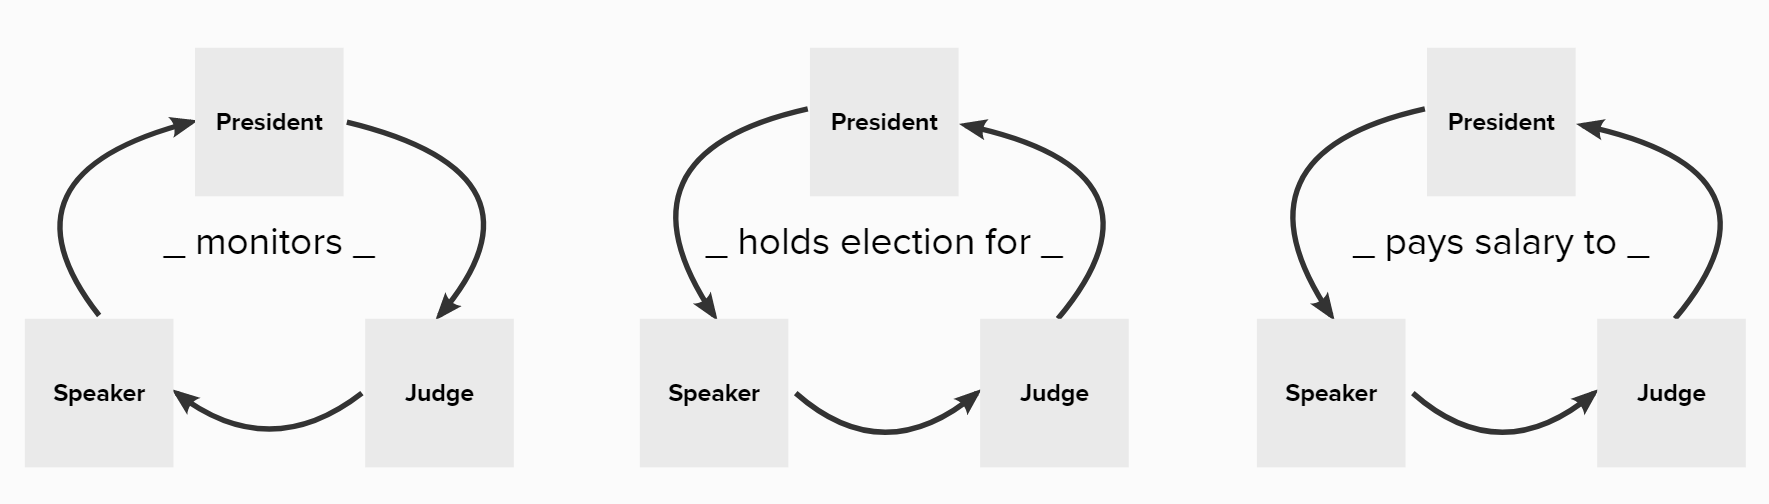
\includegraphics[scale=0.33]{05_iigo/images/role cycles.png}
\caption{Accountability cycle (left), the transfer-of-power cycle (middle) and salary cycle (right).}
\label{fig:cycles_in_IIGO}
\end{figure}


\subsection{Transfer-of-power}
\label{subsec:transfer-of-power}
\begin{enumerate}
    \item The Speaker conducts a vote for the election of the new Judge.
    \item The Judge conducts a vote for the election of the new President.
    \item The President conducts a vote for the election of the new Speaker.
\end{enumerate}
Refer to the Figure~ \ref{fig:cycles_in_IIGO} for further clarification about the transfer-of-power cycle.

\begin{rule_IIGO}
   The role $X$ has the \emph{obligation} to conduct a vote for the election of $Y$ at the end of the term (see Definition~\ref{def:term}) if and only if the role $X$ is accountable to the role $Y$. 
\end{rule_IIGO}.

\section{Budget and Salary}
\subsection{Budget}
%Actions associated with the IIGO have an associated cost that is defined as a configuration parameter. The institutional-power-enabled actions of  identified to require a "computational" component are:

Institutional-enabled-power actions in the IIGO have an associated cost with them. Some examples for such actions include:


%that is defined as a configuration parameter. The institutional-power-enabled actions of  identified to require a "computational" component are:


%We have defined the resource to be an endogenous one, hence any computation surrounding the distribution of the resource must use up some of that resource. 
\begin{itemize}
\item Calling any vote and computing the winner.
\item Declaring (e.g. \textit{announcing} the result of a vote).
\item Setting the amount of \emph{taxation} for each island.
\item Deciding the allocation distribution for each island.
\item Inspecting an island's action history.
\item Monitoring a role.
\end{itemize}

Since IIGO has been designed to act in the common good, IIGO-related costs will be directly withdrawn from the common pool. Since the common pool is considered a communal property of the archipelago, there are rules in place to limit how much each role is allowed to spend in order to perform its own institutional-power-enabled actions. This is the reason why defining the \emph{budget} and keeping it separate for each of the three IIGO roles.


As a role performs institutional-enabled-power actions, the corresponding cost associated with this action is subtracted from the role's budget. A budget of zero means that the role does not have the \emph{power} to perform any of its institutional-power-enabled actions. The removal of the budget rule from the rules in play means the role is allowed to perform as many such actions as it prefers to (as long as those actions are not governed by other rules). 



%As a role performs an endogenous-cost action, the corresponding cost associated with this action is subtracted from the role's budget. Thus, if as a result of an endogenous-cost action a role will be left with negative budget, it will have gone over the budget limit and will have broken the budget rule. A budget of zero means that the role is not allowed to perform any of its institutional-power-enabled actions associated an endogenous-cost. The removal of the budget rule from the rules in play means the role is allowed to perform as many such actions as it pleases (as long as those actions are not governed by other rules). 

The budget rule is also persistent across turns. This means that, assuming nothing else affects the budget, if a role has $100$ resources in its budget at each turn and spends only $10$ resources, this means that this very same role has $90$ resources in its budget at the next turn. On the other hand, islands can choose to increase the budget periodically every turn. This is governed by another budget extension rule.




%one turn and it spends 10, it has 90 resources in it's budget the next turn. 

Finally, it must be noted that the budget is inherently linked with the fact that whether obligations of a specific role can be undergone.
For example, during \emph{monitoring}, it should not be seen as a rule violation if a role has not acted on an obligation if it would go over the budget as a result. 

%This can also be seen as an added clause "... and the action is only permitted if they have the budget" to most rules which govern actions with an endogenous-cost.
%\begin{rule_IIGO}
    %The budget is increased by an amount $N$ every turn.
%\end{rule_IIGO}

%This rule means that, assuming nothing else affects the budget, if a budget is set to increase by 10 resources every turn and the budget is a 100 resources in turn one, the budget is 110 resources in turn 2. Setting this rule to 0 is equal to removing this rule and it means that the budget is never increased. 


\subsection{Salary}
\label{subsec:salary}
A salary is paid to each role in power as an incentive to act in a publicly approved way. %Hence, each role has the \emph{power} to pay a salary to another role following the salary cycle in Figure~\ref{fig:cycles_in_IIGO}.
\begin{rule_IIGO} \label{rule:salary}
   %Each role has the \emph{obligation} to pay the salary of amount $S$ to another if and only if the amount paid $S'$ is equal to $S$.
   Each role has the \emph{obligation} to pay the salary of amount $S$ to one another following the salary cycle in Figure~\ref{fig:cycles_in_IIGO}.
\end{rule_IIGO}

In Rule~\ref{rule:salary}, setting $S=0$ (through changing the active rules in place) means that roles do not have the permission to pay any salary. Removing the Rule~\ref{rule:salary} means that the roles may freely choose the amount $S$ for the salary payments.

\section{IIGO Session order}

\begin{enumerate}
    \item The Judge has the \emph{power} to check the history of actions to confirm whether the previously punished island(s) has/have obeyed the previous round's sanctions, meaning whether they contributed to the common pool accordingly in case of economic sanctions.
    %\begin{itemize}
      %  \item \emph{Suggested Rule:} In case of disobeying sanctions, the Judge is \emph{obliged} and \emph{permitted} to increase the severity of sanctions with respect to specific islands.
   % \end{itemize}
    \item The Judge has the \emph{power} to carry out \emph{inspections} on the history of actions of any island $X$ to check whether:
        \begin{enumerate}
        \item the reported resources of $X$ in the previous round match the real value of resources $X$ had in its private pool for the previous turn.
        \item the island $X$ has retrieved the right amount of the resources from the common pool, based on the \emph{allocation request} evaluated by the previous President.
            \begin{itemize}
            \item An example: In the previous round, the President has decided that the island $X$ can take $Y$ amount of resources from the common pool. If the Judge finds out that the island $X$ has taken an amount of $Y'$ such that $Y' > Y$, the Judge has the \emph{power} to invoke sanctions on the island $X$.
            
            %the Judge is \emph{obliged} and \emph{permitted} to sanction island $X$.
            \end{itemize}
        \end{enumerate}
    \item The Judge has the \emph{power} to invoke sanctions based on the outcome of the inspections.
    \item The President has the \emph{power} to decide to carry out a \emph{monitoring} on:
        \begin{enumerate}
        \item the sanctions imposed by the Judge.
        \end{enumerate}
    \item The islands may report the resources in their private pools to the President.
    \item The President has the \emph{power} to let each island know about the amount of \emph{taxation} they have to pay.
    \item The island has the \emph{power} to make an \emph{allocation request} to the President.
    \item The President has the \emph{power} decide on an allocation of resources and let each island know about the amount of resource allocation they are permitted to take from the common pool.
    \item The island has the \emph{power} to pick and to propose a rule to be voted on to the President.
    \item The President has the \emph{power} to choose a rule to be voted on from the received rule proposals.
    \item The Speaker has the \emph{power} to decide to carry out a \emph{monitoring} on: 
        \begin{enumerate}
        \item the resource allocation decided by the President.
        \item the rule proposed by the President.
        \end{enumerate}
    \item The Speaker has the \emph{power} to call a vote.
        \begin{enumerate}
        \item The islands vote in support of, or against, the rule (aye or nay) anonymously.
        \end{enumerate}
    \item The Speaker has the \emph{power} to announce a result of a vote to the islands and carries out the law change, if required (e.g. deleting/rejecting a rule if there is a majority nay vote).
    \item The Judge has the \emph{power} to decide to carry out \emph{monitoring} on:
        \begin{enumerate}
        \item the vote called by the Speaker.
        \item the Speaker announcing the result.
    \end{enumerate}
    \item The roles pay salary for one another following the accountability cycle in Figure~ \ref{fig:cycles_in_IIGO}.

\end{enumerate}



\section{Future Work}

\begin{itemize}
    \item \textbf{Diplomatic sanctions}: Although having the potential of being a good alternative for severer sanctions discussed in  Section~\ref{sec:sanctions}, diplomatic sanctions are \emph{not} implemented within the scope of the coursework. \\
    Suggested diplomatic sanctions include:
        \begin{itemize}
            \item Revoking an island's eligibility to vote and to be elected for a position.
            \item Revoking an island's eligibility to propose a rule/motion.
        \end{itemize}
    \item \textbf{Immutable rules}: Within the scope of the coursework, a subset of rules could have been categorised as immutable. This means that to change such immutable rules, the islands first need to vote to change their status to be \emph{mutable}, and consequently, hold another vote to change these mutable rules.
    %\item \textbf{Adding rules to the proposal list: } 
\end{itemize}

    \chapter{Inter-Island Governmental Organisation (IIGO)}


The role of IIGO is to maintain, update, and revise the rules concerning provision to managing the long-term collective risk dilemma (ltCRD). 

\begin{itemize}
    \item There will be 3 distinct branches in the IIGO: the \textbf{legislative branch}, \textbf{executive branch} and \textbf{judicial branch}\footnote{This is, as no surprise, inspired by the separation of powers in Western democracies.}.
    \item Each role is put in power according to the  transfer-of-power rules (see Section~\ref{subsec:transfer-of-power} for more detail).
    \item The head of the legislative branch is the Speaker, the head of the executive branch is the President, and the head of judicial branch is the Judge.
    \begin{itemize}
        \item  The Speaker, President and Judge are selected, through a democratic election, from the islands in the archipelago\footnote{This naming is inspired by the roles in the US Government.}.
        \item The resources gathered by the archipelago are endogenous, hence acting on the institutional powers granted to the Speaker, President or Judge costs resources. 
        \item For their duty, the President, the Speaker and the Judge receive a salary for each of their turns in office (see Section~\ref{subsec:salary} for more detail).
        \item The limit of the powers of the President, Speaker and Judge are defined in this chapter (e.g. the Speaker can only call one vote per turn).
 
    \end{itemize}
\end{itemize}

\subsection{IIGO Specific Definitions}
\begin{definition} \label{def:ballot}
    A \textbf{ballot} is related to each island's \textbf{power} to support or disagree with the rule specified in the vote called by the President and to vote in favour or against an island for a specific role (i.e. the President, Speaker, Judge) at each round of the game.
\end{definition}


%\begin{definition} \label{def:vote}
    %A \textbf{vote} is related to a role's (i.e. the President, Speaker, Judge) \textbf{power} to call a vote for a specific rule or an election.
%\end{definition}


\begin{definition} \label{def:tax}
    The \textbf{taxation} is related to the President's \textbf{power} to request a specific \underline{\textbf{minimum}} amount of contribution from each island to the common pool at each round of the game. 
\end{definition}

\begin{definition} \label{def:alloc_req}
    An \textbf{allocation request} is related to each island's \textbf{power} to request a specific amount of resource allocation from the President at each round of the game.
\end{definition}


\begin{definition} \label{def:rule_prop_list}
A \textbf{rule proposal list} is related to each island's \textbf{power} to propose a specific rule to be passed to the President at each round of the game.
\end{definition}

\begin{definition} \label{def:invst}
    An \textbf{investigation} is related to the Judge's \textbf{power} to acquire information to make a decision, followed by a calculation of the expected results and checking whether some specific rules have been obeyed, exclusively for the actions carried out by the \textbf{islands}. 
\end{definition}


An example of an \emph{investigation}: The President has permitted the island $X$ to take the amount of $Y$ resources from the common pool. Upon \emph{investigation} carried out by the Judge, it is revealed that the amount of resources taken out from the common pool by the island $X$ is, in fact, $Y'$ such that $Y' \neq Y$.


\begin{definition}
\textbf{Monitoring} is a government official's \textbf{power} to perform event recognition and to check whether some specific rules have been obeyed.
\end{definition}

An example of \emph{monitoring}: The Speaker has performed only the following action: \emph{counted the votes and calculated the result} for a rule. Upon \emph{monitoring} carried out by the President, it is noticed that the Speaker has not made any \emph{announcement}. Hence, the Speaker has not followed their obligation to \emph{announce} the result of any vote held.

See Section~\ref{sec:accountability} for more information about which roles can monitor which ones.


\begin{definition}
\textbf{Investigative-monitoring} is a government official's \textbf{power} to acquire the information used in acting on a governmental power followed by calculation of the expected results and checking whether some specific rules have been obeyed, exclusively for the actions carried out by a government official they are responsible for.
\end{definition}

An example of \emph{investigative-monitoring}: The Speaker has performed the following actions: \emph{counted the votes and calculated the result $R$} for a vote $V$ and \emph{announced} the result $R'$ for the vote $V$. Upon \emph{investigative-monitoring} carried out by the President, it is noticed that $R' \neq R$. Hence, the Speaker has modified the announced result.


\begin{definition}
The \textbf{sanction} is related to the Judge's \emph{power} to punish non-compliant islands when their disobedience is confirmed through investigations at a specific turn.
\end{definition}


\begin{definition}
The (judicial) \textbf{pardon} is related to the Judge's \emph{power} to forgive a non-compliant island at a specific turn.
\end{definition}

\begin{definition}
The \textbf{budget} is the maximum amount of resources a role is permitted to spend from the common pool as it performs its own institutional-power-enabled actions at a specific turn.
\end{definition}


\begin{definition}
The \textbf{salary} is the amount of resources a role is to be given from the common pool as a reward for performing its institutional-power-enabled actions at a specific turn.
\end{definition}

\begin{definition} \label{def:term}
A \textbf{term} is the number of turns an island is \emph{permitted} to hold a role, and after which the responsible role (indicated in the transfer-of-power cycle in Figure~\ref{fig:cycles_in_IIGO}) is \emph{obliged} to initiate transfer-of-power.
\end{definition}

\subsection{\emph{Power}, \emph{Permission} and \emph{Obligation} Distinction}
In the rest of the specifications, we will be specifically using the following three terms to define the actions and responsibilities carried out by the Speaker, President, Judge (see Figure~ \ref{fig:per_obl_sets}):
\begin{itemize}
    \item Power
    \item Permission
    \item Obligation
\end{itemize}



\begin{figure}[H] 
\centering
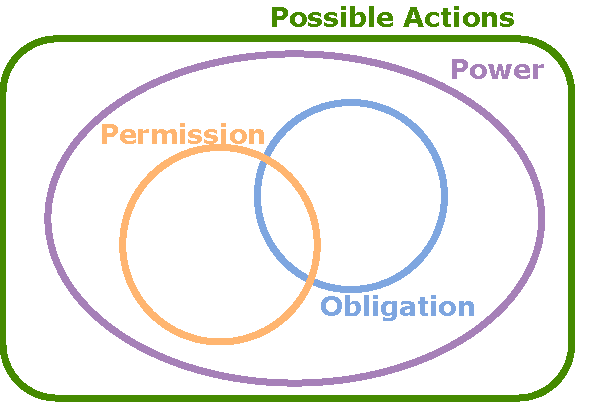
\includegraphics[width=0.6\textwidth]{05_iigo/images/SOMAS_per_obl.pdf}
\caption{Relationship between \emph{power}, \emph{permission} and \emph{obligation}.}
\label{fig:per_obl_sets}
\end{figure} 


For example, the Judge has the \emph{power} to carry out investigations at an IIGO session. There are no rules specifying which specific islands the Judge should investigate. Therefore, the Judge has the \emph{permission} to investigate any `alive' islands during a session. However, the Judge is \emph{obliged} to make at least some number of investigations each turn.



\section{Executive Branch}
\label{sec:executive}
The executive branch is responsible for \textbf{carrying out the law}.
\begin{itemize}
       
    \item The President has the \emph{power} to: 
    \begin{itemize}
        
        \item Select a rule for voting $R^{*}$ to be passed to the Speaker.
        \begin{rule_IIGO}
            The President has the \emph{obligation} to \emph{select} a rule $R^{*}$ if the \emph{rule proposal list} has at least one proposed rule in it.
        \end{rule_IIGO}
        \begin{rule_IIGO}
            The President has the \emph{permission} to \emph{select} a rule $R^{*}$ if and only if $R^{*} \in S$, where $S$ is the \emph{rule proposal list}.
        \end{rule_IIGO}
        
        \item Decide the amount of individual \emph{taxation} (i.e. a specific \emph{minimum} amount of contribution to the common pool for each island) for the current turn.
        
        \begin{itemize}
            \item The President is given the self-reported resource amounts held by each island to assist in this decision.
            %\item Suggested Rule: For any island that has chosen to not report it's resources, the President has the \emph{obligation} to set them an individual tax amount T.
        \end{itemize}
        
        \item Decide the allocation of resources distributed from the common pool to the islands (i.e. a specific \emph{maximum} amount an island is permitted to take from the common pool).
        
        \begin{itemize}
            \item The President is given the \emph{allocation requests} made by each island.
            %\item \emph{}{Suggested Rule:} The President has an obligation to prioritise islands in critical condition.
        \end{itemize}
    \end{itemize}
\end{itemize}



\section{Legislative Branch}
\label{sec:legislative}
The legislative branch is responsible for \textbf{making the law}.
\begin{itemize}

    \item The Speaker has the \emph{power} to:
    \begin{itemize}
        
        \item Call a vote $V$ for a rule $R$.
        \begin{rule_IIGO}
            The Speaker has the \emph{obligation} to \emph{call} a vote $V$ if and only if the President has \emph{selected} a rule $R$ to be voted on.
        \end {rule_IIGO}
        \begin{rule_IIGO}
            The Speaker has the \emph{permission} to \emph{call} a vote $V$ for a rule $R$ if and only if the rule $R = R^{*}$, where $R^{*}$ is the rule \emph{selected} by the President.
        \end {rule_IIGO}
            
        \item Choose which islands are participating in the vote $V$.
       % \footnote{This is our sequential implementation alternative for the power to close the ballot box.}.
        \begin{rule_IIGO}
            The Speaker has the \emph{obligation} to ask for a vote from all alive islands.
        \end {rule_IIGO}
            
        \item Declare the result $C$ of a vote $V$. 
        \begin{rule_IIGO}
            The Speaker has the \emph{obligation} to \emph{declare the result} $C$ for a vote $V$ if and only if the vote V has been \emph{called}.
        \end {rule_IIGO}
        \begin{rule_IIGO}
            The Speaker has the \emph{permission} to \emph{declare the result} $C$ for a vote $V$ if $C = C^{*}$, where $C^{*}$ is the result produced by \emph{calling} the vote $V$.
        \end {rule_IIGO}
        \begin{itemize}
            \item This step is what enables a rule to be \emph{active}.
        \end{itemize}
    \end{itemize}
\end{itemize}




\section{Judicial Branch}
\label{sec:judicial}

The judicial branch is responsible for \textbf{evaluating the law}.
\begin{itemize}
    \item The Judge has the \emph{power} to:
    \begin{itemize}
        \item Perform a number of \emph{inspections}\footnote{An \emph{inspection} \textbf{costs} an expense of resources (See Definition~\ref{def:invst} for more detail).} $I$ and produce a compliance outcome $\mathbb{O}^{*}$\footnote{Note that the compliance outcome $\mathbb{O}^{*}$ considered is a boolean.}.
        %(true: the island has been compliant with the rules in play, false: the island has not been compliant with the rules in play)
        %\begin{itemize}
           % \item For example, to check if the event outcome is \emph{concurrent}\footnote{Again, what is defined as "concurrent"? A clear definition is needed.} with the rules.
        %\end{itemize}
        \begin{rule_IIGO}
            The Judge has the \emph{obligation} to make at least $N$ investigations at each turn.
        \end{rule_IIGO}
        \item Declare the outcome $\mathbb{O}$ of an inspection $I$ to all islands\footnote{This act of broadcasting is especially important for islands to form an opinion about the sanctioned islands accordingly.}.
        \begin{rule_IIGO}
            The Judge has the \emph{obligation} to declare the outcome $\mathbb{O}$ of an inspection $I$ if and only if the inspection $I$ has been performed.
        \end{rule_IIGO}
        \begin{rule_IIGO}
            The Judge has the \emph{permission} to declare the outcome $\mathbb{O}$ of an inspection $I$ if $\mathbb{O} = \mathbb{O}^{*}$, where $\mathbb{O}^{*}$ is the outcome of the inspection $I$.
        \end{rule_IIGO}
        %\item Initiate the removal of the \texttt{President}.
        %\begin{itemize}
            %\item A good Judge would be especially vigilant during \emph{power transfer} regarding the \emph{President} position (see Section~\ref{leg_const} for more detail).
        %\end{itemize}
        \item Invoke economic \textbf{sanctions} (see Section~\ref{sec:sanctions} for more detail).
        \begin{rule_IIGO}
            The Judge has the \emph{obligation} to invoke a sanction $S$ for an island $X$ if and only if an investigation $I$ has an outcome $\mathbb{O}^{*}$ indicating non-compliance, and $I$ is an investigation of an action taken by island $X$.
        \end{rule_IIGO}
        \item Invoke even more severe sanctions in the case of further disobedience to previous sanction(s).
        \begin{rule_IIGO}
            The Judge has the \emph{permission} to invoke a severer sanction $S'$ for an island $X$ if the island $X$ has not fulfilled the requirements of the previous sanction $S$.
        \end{rule_IIGO}
        \item Pardon the islands which are currently sanctioned.
        \begin{rule_IIGO}
            The Judge has the \emph{permission} to revoke any sanction $S$ of an island $X$ at a specific turn.
        \end{rule_IIGO}
    \end{itemize}
\end{itemize}
%(e.g. a new rule that falls under a "sanction" category \hl{[I'm not sure about this being a `new rule` [Ezgi]]}

\subsection{Sanctions}
\label{sec:sanctions}
All sanctions are of economic nature which include:
        \begin{itemize}
            %\item Revoking an island's access to the common pool.
            \item Enforcing an island to contribute a specific amount of resources to the common pool.
            \begin{itemize}
                \item This does not mean that the Judge has the \emph{power} to take resources from an island in order to put them to the common pool -- the island itself is expected to carry out this implication imposed by the sanction itself, otherwise further punishment can be induced by the Judge.
                \item Similarly, \emph{opinion formulation} will follow accordingly whether the island(s) is/are following the implications imposed by the sanction(s).
            \end{itemize}
        
    \end{itemize}
    Sanctions are the associated penalty that comes with an island breaking a specific rule. The Judge is in full control of the penalties associated with breaking any rules. Once the Judge has specified the score of the penalty associated with each time an island breaks a rule, the cumulative penalties accumulated by the island are then used to determine which \textbf{sanction tier} that each island falls into. The score threshold to determine the boundaries of the sanction tiers are set by the Judge. At each turn of the game, each island is told whether they are being sanctioned, and if so, which \textbf{sanction tier} that they are currently in. The \textbf{sanction tiers} of the non-compliant islands are also broadcasted to the other islands in the archipelago. To summarise, the sanctioning process follows these steps:
    
    
    
    %Sanctions are based on an island breaking a rule. Each rule must therefore have an associated penalty. By default, we set these penalties such that they add $1$ to the total sanction score for each island. However, we allow the judge to override this scoring, the judge is able to set their own scores for any particular rule as they desire. This custom scoring is then used when an island breaks a particular rule. By looking at events that occurred in the last turn, and using the customised scoring we provide the holder of the judge role with full control of the penalties for breaking any rules.
    
    





%we then use the cumulative penalties accumulated by each island to determine which Sanction Tier they fall into. The score threshold's required to fall into these sanction tiers is set by the judge and is checked for monotonicity. Each island is told whether they are being sanctioned, and is so what tier they are in. We also tell other islands about which sanction tiers other islands have fallen into. 

    \begin{enumerate}
        \item The Judge has the \emph{power} to set custom penalties associated with breaking any rules.
        \item The Judge is given a list of all events that occurred in the previous turn.
        \item The Judge has the \emph{power} to check whether any, or all of these previous events, involve the islands in the archipelago breaking any rules.
        \item Each of the transgressions is scored using the Judge's custom penalties if the Judge has set them. Otherwise, a score of $1$ is given each time a rule is broken.
        \item The Judge has the \emph{power} to revise the sanction thresholds.
        \item Using the latest sanction thresholds available, each island is assigned to a sanction tier based on the sanction score that it has received.
        \item These sanction tiers are broadcasted to all of the islands in the archipelago.
        \item The Judge then uses sanctions rules in place to calculate the specific amount of resources that each non-compliant island has in order to determine how much it should contribute to the common pool, based on the sanction tier that it is in.
    \end{enumerate}



\section{Constitutional Rights and Obligations in the Archipelago}
\label{sec:const_rights_obl_archi}
Each island has the \emph{power} to:
\begin{itemize}
\item make an \emph{allocation request} (see Definition~\ref{def:alloc_req}) to the President for a specific amount to be allocated to them.
\item report the number of resources it is in possession of to the President.
\begin{rule_IIGO}
    Each island has the \emph{obligation} to report the number of resources it is in possession of to the President.
\end{rule_IIGO}
\begin{rule_IIGO}
    Each island has the \emph{permission} to report the number of resources $R'$ if and only if $R' = R$, where R is the number of resources the island is in possession of.
\end{rule_IIGO}
\item take resources from the common pool.


\begin{rule_IIGO}
    Each island has the \emph{permission} to take at maximum $N$ resources, where $N$ is the specific allocation made by the President to that island\footnote{If no such allocation is made, the island is \emph{permitted} to take any amount of resources.}.
\end{rule_IIGO}
\item contribute resources to the common pool.
\begin{rule_IIGO}
    Each island has the \emph{obligation} to contribute to the common pool an amount greater or equal to that of the individual tax set by the President.
\end{rule_IIGO}
                %The President is in
                %(unless there is a rule in place that dictates how Speaker is to allocate resources).
\item add a rule to the \emph{rule proposal list} (see Definition~\ref{def:rule_prop_list}) at the start of each turn.
        %\begin{itemize}
            %\item The game specification includes how many rules an island can propose each turn.
        %\end{itemize}
        %\item vote  for rules in the Legislative Branch and vote for their favourite islands in elections
\item participate in the legislative branch of the government by casting ballots in votes called by the Speaker
\item vote for an island to be elected for a specific role (e.g. the President, Judge, Speaker) during the elections\footnote{This will be assumed to be true \underline{unless stated otherwise}. %Note that \textbf{diplomatic sanctions} can disable this power of a specific island (see Section~\ref{jud_const}).}.
        }.
\end{itemize}
\section{Accountability Cycle}
\label{sec:accountability}


To ensure that the government avoids corruption and abuse of power, each branch is accountable to another. The President is accountable to the Speaker, the Speaker is accountable to the Judge, and the Judge is accountable to the President (see Figure~ \ref{fig:cycles_in_IIGO}). This accountability cycle is enacted through \emph{monitoring} actions\footnote{Note that the terms \textbf{monitoring} and \textbf{investigation} have similar but quite different meanings in the IIGO context.}. 

The powers related to the accountability cycle and transfer-of-power for each role can be summarized as the following: 
\begin{itemize}
    \item The Speaker has the \emph{power} to: 
    \begin{itemize}
        \item monitor the President.
        \item announce the result of this monitoring.
        \item initiate the transfer-of-power for the Judge.
    \end{itemize}
    \item The President has the \emph{power} to: 
    \begin{itemize}
        \item monitor the Judge.
        \item announce the result of this monitoring.
        \item initiate the transfer-of-power for the Speaker.
    \end{itemize}
    \item The Judge has the \emph{power} to: 
    \begin{itemize}
        \item  monitor the Speaker.
        \item announce the result of this monitoring.
        \item initiate the transfer-of-power for the President.
    \end{itemize}
\end{itemize}

%Unlike investigations performed by the Judge, who performs investigations on island actions in the following turn, each role is given the opportunity to check up on the actions of the role it is responsible for immediately after they have been performed. In this sense, the President can monitor (includes investigative-monitoring) the powers (calling a vote and announcing the result) acted on by the Speaker immediately after the Speaker's announcement (or lack there of). The government officials hold a lot of power so this is to ensure that any wrong-doing is determined as quickly as possible. For this project we are only pursuing one degree of monitoring, that is, the powers relating to the accountability cycle will not be monitored themselves. We assume that agents will act in the interest of themselves and keeping all the islands alive is beneficial to everyone. Hence, while the agents might be inclined to break rules in order to benefit themselves, anyone else breaking the rules is seen as undesirable under the assumption that the system in place is there to benefit all. 


Through the proposed accountability cycle, each role is given the opportunity to check up on the actions of the role it is accountable for immediately after they have been performed. It is clear that the IIGO roles (i.e. the President, Speaker and Judge) hold a considerable amount of \emph{power} in their hands. The accountability cycle is designed to address the possible abuses of this power. With monitoring, any wrong-doing in the IGO is determined as quickly as possible and the role in question can be replaced. 

Within the scope of the coursework, we decided to pursue only \emph{one degree of monitoring}, meaning that the powers relating to the accountability cycle will not be monitored themselves. We assume that agents will act in the interest of all the islands in the archipelago. Hence, while the agents might be inclined to break the rules to benefit in some form, it is assumed that the others will negatively see any non-compliant islands based on the assumption that the proposed IIGO system is in place to maintain the welfare of all the islands.

Let role $X$ be accountable to the role $Y$, which is accountable to the role $Z$. Then:
\begin{rule_IIGO}
$Y$ has the \emph{obligation} to declare the outcome of the monitoring result $M$ associated with the action $A$ undertaken by $X$ if and only if $Y$ has monitored the action $A$ performed by $X$. 
\end{rule_IIGO}
\begin{rule_IIGO}
$Y$ has the \emph{permission} to declare the monitoring result $M$ associated with the action $A$ undertaken by $X$ if and only if $M = M^{*}$, where $M^{*}$ is the outcome of \emph{monitoring} action $A$ performed by $X$\footnote{These constitutional rules should be available to the agents to check their decision against. However, due to having only one degree of accountability cycle in place, these rules are not enforced through any sanctions (i.e. breaking these rules has no consequences as they only deem to be an \emph{agreement} among the roles).}.
\end{rule_IIGO}


\begin{figure}[!htb]
\centering
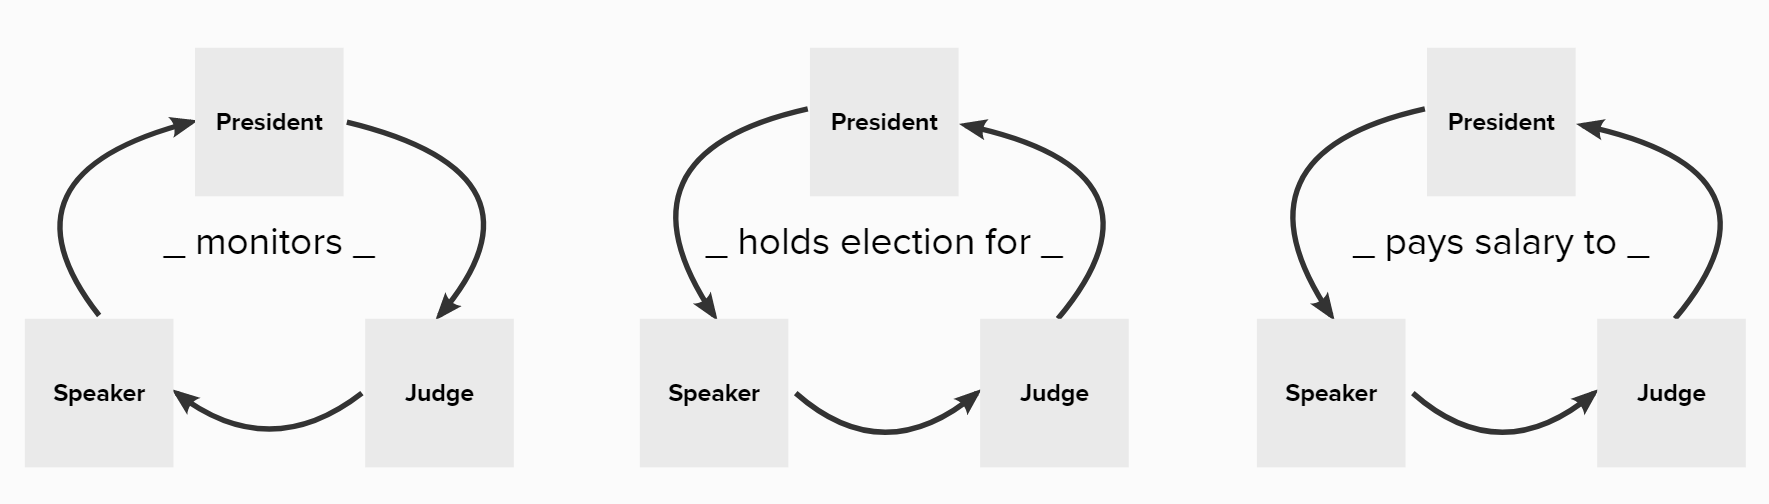
\includegraphics[scale=0.33]{05_iigo/images/role cycles.png}
\caption{Accountability cycle (left), the transfer-of-power cycle (middle) and salary cycle (right).}
\label{fig:cycles_in_IIGO}
\end{figure}


\subsection{Transfer-of-power}
\label{subsec:transfer-of-power}
\begin{enumerate}
    \item The Speaker conducts a vote for the election of the new Judge.
    \item The Judge conducts a vote for the election of the new President.
    \item The President conducts a vote for the election of the new Speaker.
\end{enumerate}
Refer to the Figure~ \ref{fig:cycles_in_IIGO} for further clarification about the transfer-of-power cycle.

\begin{rule_IIGO}
   The role $X$ has the \emph{obligation} to conduct a vote for the election of $Y$ at the end of the term (see Definition~\ref{def:term}) if and only if the role $X$ is accountable to the role $Y$. 
\end{rule_IIGO}.

\section{Budget and Salary}
\subsection{Budget}
%Actions associated with the IIGO have an associated cost that is defined as a configuration parameter. The institutional-power-enabled actions of  identified to require a "computational" component are:

Institutional-enabled-power actions in the IIGO have an associated cost with them. Some examples for such actions include:


%that is defined as a configuration parameter. The institutional-power-enabled actions of  identified to require a "computational" component are:


%We have defined the resource to be an endogenous one, hence any computation surrounding the distribution of the resource must use up some of that resource. 
\begin{itemize}
\item Calling any vote and computing the winner.
\item Declaring (e.g. \textit{announcing} the result of a vote).
\item Setting the amount of \emph{taxation} for each island.
\item Deciding the allocation distribution for each island.
\item Inspecting an island's action history.
\item Monitoring a role.
\end{itemize}

Since IIGO has been designed to act in the common good, IIGO-related costs will be directly withdrawn from the common pool. Since the common pool is considered a communal property of the archipelago, there are rules in place to limit how much each role is allowed to spend in order to perform its own institutional-power-enabled actions. This is the reason why defining the \emph{budget} and keeping it separate for each of the three IIGO roles.


As a role performs institutional-enabled-power actions, the corresponding cost associated with this action is subtracted from the role's budget. A budget of zero means that the role does not have the \emph{power} to perform any of its institutional-power-enabled actions. The removal of the budget rule from the rules in play means the role is allowed to perform as many such actions as it prefers to (as long as those actions are not governed by other rules). 



%As a role performs an endogenous-cost action, the corresponding cost associated with this action is subtracted from the role's budget. Thus, if as a result of an endogenous-cost action a role will be left with negative budget, it will have gone over the budget limit and will have broken the budget rule. A budget of zero means that the role is not allowed to perform any of its institutional-power-enabled actions associated an endogenous-cost. The removal of the budget rule from the rules in play means the role is allowed to perform as many such actions as it pleases (as long as those actions are not governed by other rules). 

The budget rule is also persistent across turns. This means that, assuming nothing else affects the budget, if a role has $100$ resources in its budget at each turn and spends only $10$ resources, this means that this very same role has $90$ resources in its budget at the next turn. On the other hand, islands can choose to increase the budget periodically every turn. This is governed by another budget extension rule.




%one turn and it spends 10, it has 90 resources in it's budget the next turn. 

Finally, it must be noted that the budget is inherently linked with the fact that whether obligations of a specific role can be undergone.
For example, during \emph{monitoring}, it should not be seen as a rule violation if a role has not acted on an obligation if it would go over the budget as a result. 

%This can also be seen as an added clause "... and the action is only permitted if they have the budget" to most rules which govern actions with an endogenous-cost.
%\begin{rule_IIGO}
    %The budget is increased by an amount $N$ every turn.
%\end{rule_IIGO}

%This rule means that, assuming nothing else affects the budget, if a budget is set to increase by 10 resources every turn and the budget is a 100 resources in turn one, the budget is 110 resources in turn 2. Setting this rule to 0 is equal to removing this rule and it means that the budget is never increased. 


\subsection{Salary}
\label{subsec:salary}
A salary is paid to each role in power as an incentive to act in a publicly approved way. %Hence, each role has the \emph{power} to pay a salary to another role following the salary cycle in Figure~\ref{fig:cycles_in_IIGO}.
\begin{rule_IIGO} \label{rule:salary}
   %Each role has the \emph{obligation} to pay the salary of amount $S$ to another if and only if the amount paid $S'$ is equal to $S$.
   Each role has the \emph{obligation} to pay the salary of amount $S$ to one another following the salary cycle in Figure~\ref{fig:cycles_in_IIGO}.
\end{rule_IIGO}

In Rule~\ref{rule:salary}, setting $S=0$ (through changing the active rules in place) means that roles do not have the permission to pay any salary. Removing the Rule~\ref{rule:salary} means that the roles may freely choose the amount $S$ for the salary payments.

\section{IIGO Session order}

\begin{enumerate}
    \item The Judge has the \emph{power} to check the history of actions to confirm whether the previously punished island(s) has/have obeyed the previous round's sanctions, meaning whether they contributed to the common pool accordingly in case of economic sanctions.
    %\begin{itemize}
      %  \item \emph{Suggested Rule:} In case of disobeying sanctions, the Judge is \emph{obliged} and \emph{permitted} to increase the severity of sanctions with respect to specific islands.
   % \end{itemize}
    \item The Judge has the \emph{power} to carry out \emph{inspections} on the history of actions of any island $X$ to check whether:
        \begin{enumerate}
        \item the reported resources of $X$ in the previous round match the real value of resources $X$ had in its private pool for the previous turn.
        \item the island $X$ has retrieved the right amount of the resources from the common pool, based on the \emph{allocation request} evaluated by the previous President.
            \begin{itemize}
            \item An example: In the previous round, the President has decided that the island $X$ can take $Y$ amount of resources from the common pool. If the Judge finds out that the island $X$ has taken an amount of $Y'$ such that $Y' > Y$, the Judge has the \emph{power} to invoke sanctions on the island $X$.
            
            %the Judge is \emph{obliged} and \emph{permitted} to sanction island $X$.
            \end{itemize}
        \end{enumerate}
    \item The Judge has the \emph{power} to invoke sanctions based on the outcome of the inspections.
    \item The President has the \emph{power} to decide to carry out a \emph{monitoring} on:
        \begin{enumerate}
        \item the sanctions imposed by the Judge.
        \end{enumerate}
    \item The islands may report the resources in their private pools to the President.
    \item The President has the \emph{power} to let each island know about the amount of \emph{taxation} they have to pay.
    \item The island has the \emph{power} to make an \emph{allocation request} to the President.
    \item The President has the \emph{power} decide on an allocation of resources and let each island know about the amount of resource allocation they are permitted to take from the common pool.
    \item The island has the \emph{power} to pick and to propose a rule to be voted on to the President.
    \item The President has the \emph{power} to choose a rule to be voted on from the received rule proposals.
    \item The Speaker has the \emph{power} to decide to carry out a \emph{monitoring} on: 
        \begin{enumerate}
        \item the resource allocation decided by the President.
        \item the rule proposed by the President.
        \end{enumerate}
    \item The Speaker has the \emph{power} to call a vote.
        \begin{enumerate}
        \item The islands vote in support of, or against, the rule (aye or nay) anonymously.
        \end{enumerate}
    \item The Speaker has the \emph{power} to announce a result of a vote to the islands and carries out the law change, if required (e.g. deleting/rejecting a rule if there is a majority nay vote).
    \item The Judge has the \emph{power} to decide to carry out \emph{monitoring} on:
        \begin{enumerate}
        \item the vote called by the Speaker.
        \item the Speaker announcing the result.
    \end{enumerate}
    \item The roles pay salary for one another following the accountability cycle in Figure~ \ref{fig:cycles_in_IIGO}.

\end{enumerate}



\section{Future Work}

\begin{itemize}
    \item \textbf{Diplomatic sanctions}: Although having the potential of being a good alternative for severer sanctions discussed in  Section~\ref{sec:sanctions}, diplomatic sanctions are \emph{not} implemented within the scope of the coursework. \\
    Suggested diplomatic sanctions include:
        \begin{itemize}
            \item Revoking an island's eligibility to vote and to be elected for a position.
            \item Revoking an island's eligibility to propose a rule/motion.
        \end{itemize}
    \item \textbf{Immutable rules}: Within the scope of the coursework, a subset of rules could have been categorised as immutable. This means that to change such immutable rules, the islands first need to vote to change their status to be \emph{mutable}, and consequently, hold another vote to change these mutable rules.
    %\item \textbf{Adding rules to the proposal list: } 
\end{itemize}

    \chapter{Inter-Island Governmental Organisation (IIGO)}


The role of IIGO is to maintain, update, and revise the rules concerning provision to managing the long-term collective risk dilemma (ltCRD). 

\begin{itemize}
    \item There will be 3 distinct branches in the IIGO: the \textbf{legislative branch}, \textbf{executive branch} and \textbf{judicial branch}\footnote{This is, as no surprise, inspired by the separation of powers in Western democracies.}.
    \item Each role is put in power according to the  transfer-of-power rules (see Section~\ref{subsec:transfer-of-power} for more detail).
    \item The head of the legislative branch is the Speaker, the head of the executive branch is the President, and the head of judicial branch is the Judge.
    \begin{itemize}
        \item  The Speaker, President and Judge are selected, through a democratic election, from the islands in the archipelago\footnote{This naming is inspired by the roles in the US Government.}.
        \item The resources gathered by the archipelago are endogenous, hence acting on the institutional powers granted to the Speaker, President or Judge costs resources. 
        \item For their duty, the President, the Speaker and the Judge receive a salary for each of their turns in office (see Section~\ref{subsec:salary} for more detail).
        \item The limit of the powers of the President, Speaker and Judge are defined in this chapter (e.g. the Speaker can only call one vote per turn).
 
    \end{itemize}
\end{itemize}

\subsection{IIGO Specific Definitions}
\begin{definition} \label{def:ballot}
    A \textbf{ballot} is related to each island's \textbf{power} to support or disagree with the rule specified in the vote called by the President and to vote in favour or against an island for a specific role (i.e. the President, Speaker, Judge) at each round of the game.
\end{definition}


%\begin{definition} \label{def:vote}
    %A \textbf{vote} is related to a role's (i.e. the President, Speaker, Judge) \textbf{power} to call a vote for a specific rule or an election.
%\end{definition}


\begin{definition} \label{def:tax}
    The \textbf{taxation} is related to the President's \textbf{power} to request a specific \underline{\textbf{minimum}} amount of contribution from each island to the common pool at each round of the game. 
\end{definition}

\begin{definition} \label{def:alloc_req}
    An \textbf{allocation request} is related to each island's \textbf{power} to request a specific amount of resource allocation from the President at each round of the game.
\end{definition}


\begin{definition} \label{def:rule_prop_list}
A \textbf{rule proposal list} is related to each island's \textbf{power} to propose a specific rule to be passed to the President at each round of the game.
\end{definition}

\begin{definition} \label{def:invst}
    An \textbf{investigation} is related to the Judge's \textbf{power} to acquire information to make a decision, followed by a calculation of the expected results and checking whether some specific rules have been obeyed, exclusively for the actions carried out by the \textbf{islands}. 
\end{definition}


An example of an \emph{investigation}: The President has permitted the island $X$ to take the amount of $Y$ resources from the common pool. Upon \emph{investigation} carried out by the Judge, it is revealed that the amount of resources taken out from the common pool by the island $X$ is, in fact, $Y'$ such that $Y' \neq Y$.


\begin{definition}
\textbf{Monitoring} is a government official's \textbf{power} to perform event recognition and to check whether some specific rules have been obeyed.
\end{definition}

An example of \emph{monitoring}: The Speaker has performed only the following action: \emph{counted the votes and calculated the result} for a rule. Upon \emph{monitoring} carried out by the President, it is noticed that the Speaker has not made any \emph{announcement}. Hence, the Speaker has not followed their obligation to \emph{announce} the result of any vote held.

See Section~\ref{sec:accountability} for more information about which roles can monitor which ones.


\begin{definition}
\textbf{Investigative-monitoring} is a government official's \textbf{power} to acquire the information used in acting on a governmental power followed by calculation of the expected results and checking whether some specific rules have been obeyed, exclusively for the actions carried out by a government official they are responsible for.
\end{definition}

An example of \emph{investigative-monitoring}: The Speaker has performed the following actions: \emph{counted the votes and calculated the result $R$} for a vote $V$ and \emph{announced} the result $R'$ for the vote $V$. Upon \emph{investigative-monitoring} carried out by the President, it is noticed that $R' \neq R$. Hence, the Speaker has modified the announced result.


\begin{definition}
The \textbf{sanction} is related to the Judge's \emph{power} to punish non-compliant islands when their disobedience is confirmed through investigations at a specific turn.
\end{definition}


\begin{definition}
The (judicial) \textbf{pardon} is related to the Judge's \emph{power} to forgive a non-compliant island at a specific turn.
\end{definition}

\begin{definition}
The \textbf{budget} is the maximum amount of resources a role is permitted to spend from the common pool as it performs its own institutional-power-enabled actions at a specific turn.
\end{definition}


\begin{definition}
The \textbf{salary} is the amount of resources a role is to be given from the common pool as a reward for performing its institutional-power-enabled actions at a specific turn.
\end{definition}

\begin{definition} \label{def:term}
A \textbf{term} is the number of turns an island is \emph{permitted} to hold a role, and after which the responsible role (indicated in the transfer-of-power cycle in Figure~\ref{fig:cycles_in_IIGO}) is \emph{obliged} to initiate transfer-of-power.
\end{definition}

\subsection{\emph{Power}, \emph{Permission} and \emph{Obligation} Distinction}
In the rest of the specifications, we will be specifically using the following three terms to define the actions and responsibilities carried out by the Speaker, President, Judge (see Figure~ \ref{fig:per_obl_sets}):
\begin{itemize}
    \item Power
    \item Permission
    \item Obligation
\end{itemize}



\begin{figure}[H] 
\centering
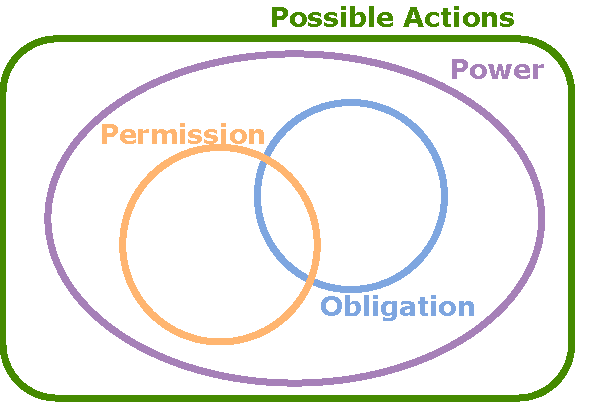
\includegraphics[width=0.6\textwidth]{05_iigo/images/SOMAS_per_obl.pdf}
\caption{Relationship between \emph{power}, \emph{permission} and \emph{obligation}.}
\label{fig:per_obl_sets}
\end{figure} 


For example, the Judge has the \emph{power} to carry out investigations at an IIGO session. There are no rules specifying which specific islands the Judge should investigate. Therefore, the Judge has the \emph{permission} to investigate any `alive' islands during a session. However, the Judge is \emph{obliged} to make at least some number of investigations each turn.



\section{Executive Branch}
\label{sec:executive}
The executive branch is responsible for \textbf{carrying out the law}.
\begin{itemize}
       
    \item The President has the \emph{power} to: 
    \begin{itemize}
        
        \item Select a rule for voting $R^{*}$ to be passed to the Speaker.
        \begin{rule_IIGO}
            The President has the \emph{obligation} to \emph{select} a rule $R^{*}$ if the \emph{rule proposal list} has at least one proposed rule in it.
        \end{rule_IIGO}
        \begin{rule_IIGO}
            The President has the \emph{permission} to \emph{select} a rule $R^{*}$ if and only if $R^{*} \in S$, where $S$ is the \emph{rule proposal list}.
        \end{rule_IIGO}
        
        \item Decide the amount of individual \emph{taxation} (i.e. a specific \emph{minimum} amount of contribution to the common pool for each island) for the current turn.
        
        \begin{itemize}
            \item The President is given the self-reported resource amounts held by each island to assist in this decision.
            %\item Suggested Rule: For any island that has chosen to not report it's resources, the President has the \emph{obligation} to set them an individual tax amount T.
        \end{itemize}
        
        \item Decide the allocation of resources distributed from the common pool to the islands (i.e. a specific \emph{maximum} amount an island is permitted to take from the common pool).
        
        \begin{itemize}
            \item The President is given the \emph{allocation requests} made by each island.
            %\item \emph{}{Suggested Rule:} The President has an obligation to prioritise islands in critical condition.
        \end{itemize}
    \end{itemize}
\end{itemize}



\section{Legislative Branch}
\label{sec:legislative}
The legislative branch is responsible for \textbf{making the law}.
\begin{itemize}

    \item The Speaker has the \emph{power} to:
    \begin{itemize}
        
        \item Call a vote $V$ for a rule $R$.
        \begin{rule_IIGO}
            The Speaker has the \emph{obligation} to \emph{call} a vote $V$ if and only if the President has \emph{selected} a rule $R$ to be voted on.
        \end {rule_IIGO}
        \begin{rule_IIGO}
            The Speaker has the \emph{permission} to \emph{call} a vote $V$ for a rule $R$ if and only if the rule $R = R^{*}$, where $R^{*}$ is the rule \emph{selected} by the President.
        \end {rule_IIGO}
            
        \item Choose which islands are participating in the vote $V$.
       % \footnote{This is our sequential implementation alternative for the power to close the ballot box.}.
        \begin{rule_IIGO}
            The Speaker has the \emph{obligation} to ask for a vote from all alive islands.
        \end {rule_IIGO}
            
        \item Declare the result $C$ of a vote $V$. 
        \begin{rule_IIGO}
            The Speaker has the \emph{obligation} to \emph{declare the result} $C$ for a vote $V$ if and only if the vote V has been \emph{called}.
        \end {rule_IIGO}
        \begin{rule_IIGO}
            The Speaker has the \emph{permission} to \emph{declare the result} $C$ for a vote $V$ if $C = C^{*}$, where $C^{*}$ is the result produced by \emph{calling} the vote $V$.
        \end {rule_IIGO}
        \begin{itemize}
            \item This step is what enables a rule to be \emph{active}.
        \end{itemize}
    \end{itemize}
\end{itemize}




\section{Judicial Branch}
\label{sec:judicial}

The judicial branch is responsible for \textbf{evaluating the law}.
\begin{itemize}
    \item The Judge has the \emph{power} to:
    \begin{itemize}
        \item Perform a number of \emph{inspections}\footnote{An \emph{inspection} \textbf{costs} an expense of resources (See Definition~\ref{def:invst} for more detail).} $I$ and produce a compliance outcome $\mathbb{O}^{*}$\footnote{Note that the compliance outcome $\mathbb{O}^{*}$ considered is a boolean.}.
        %(true: the island has been compliant with the rules in play, false: the island has not been compliant with the rules in play)
        %\begin{itemize}
           % \item For example, to check if the event outcome is \emph{concurrent}\footnote{Again, what is defined as "concurrent"? A clear definition is needed.} with the rules.
        %\end{itemize}
        \begin{rule_IIGO}
            The Judge has the \emph{obligation} to make at least $N$ investigations at each turn.
        \end{rule_IIGO}
        \item Declare the outcome $\mathbb{O}$ of an inspection $I$ to all islands\footnote{This act of broadcasting is especially important for islands to form an opinion about the sanctioned islands accordingly.}.
        \begin{rule_IIGO}
            The Judge has the \emph{obligation} to declare the outcome $\mathbb{O}$ of an inspection $I$ if and only if the inspection $I$ has been performed.
        \end{rule_IIGO}
        \begin{rule_IIGO}
            The Judge has the \emph{permission} to declare the outcome $\mathbb{O}$ of an inspection $I$ if $\mathbb{O} = \mathbb{O}^{*}$, where $\mathbb{O}^{*}$ is the outcome of the inspection $I$.
        \end{rule_IIGO}
        %\item Initiate the removal of the \texttt{President}.
        %\begin{itemize}
            %\item A good Judge would be especially vigilant during \emph{power transfer} regarding the \emph{President} position (see Section~\ref{leg_const} for more detail).
        %\end{itemize}
        \item Invoke economic \textbf{sanctions} (see Section~\ref{sec:sanctions} for more detail).
        \begin{rule_IIGO}
            The Judge has the \emph{obligation} to invoke a sanction $S$ for an island $X$ if and only if an investigation $I$ has an outcome $\mathbb{O}^{*}$ indicating non-compliance, and $I$ is an investigation of an action taken by island $X$.
        \end{rule_IIGO}
        \item Invoke even more severe sanctions in the case of further disobedience to previous sanction(s).
        \begin{rule_IIGO}
            The Judge has the \emph{permission} to invoke a severer sanction $S'$ for an island $X$ if the island $X$ has not fulfilled the requirements of the previous sanction $S$.
        \end{rule_IIGO}
        \item Pardon the islands which are currently sanctioned.
        \begin{rule_IIGO}
            The Judge has the \emph{permission} to revoke any sanction $S$ of an island $X$ at a specific turn.
        \end{rule_IIGO}
    \end{itemize}
\end{itemize}
%(e.g. a new rule that falls under a "sanction" category \hl{[I'm not sure about this being a `new rule` [Ezgi]]}

\subsection{Sanctions}
\label{sec:sanctions}
All sanctions are of economic nature which include:
        \begin{itemize}
            %\item Revoking an island's access to the common pool.
            \item Enforcing an island to contribute a specific amount of resources to the common pool.
            \begin{itemize}
                \item This does not mean that the Judge has the \emph{power} to take resources from an island in order to put them to the common pool -- the island itself is expected to carry out this implication imposed by the sanction itself, otherwise further punishment can be induced by the Judge.
                \item Similarly, \emph{opinion formulation} will follow accordingly whether the island(s) is/are following the implications imposed by the sanction(s).
            \end{itemize}
        
    \end{itemize}
    Sanctions are the associated penalty that comes with an island breaking a specific rule. The Judge is in full control of the penalties associated with breaking any rules. Once the Judge has specified the score of the penalty associated with each time an island breaks a rule, the cumulative penalties accumulated by the island are then used to determine which \textbf{sanction tier} that each island falls into. The score threshold to determine the boundaries of the sanction tiers are set by the Judge. At each turn of the game, each island is told whether they are being sanctioned, and if so, which \textbf{sanction tier} that they are currently in. The \textbf{sanction tiers} of the non-compliant islands are also broadcasted to the other islands in the archipelago. To summarise, the sanctioning process follows these steps:
    
    
    
    %Sanctions are based on an island breaking a rule. Each rule must therefore have an associated penalty. By default, we set these penalties such that they add $1$ to the total sanction score for each island. However, we allow the judge to override this scoring, the judge is able to set their own scores for any particular rule as they desire. This custom scoring is then used when an island breaks a particular rule. By looking at events that occurred in the last turn, and using the customised scoring we provide the holder of the judge role with full control of the penalties for breaking any rules.
    
    





%we then use the cumulative penalties accumulated by each island to determine which Sanction Tier they fall into. The score threshold's required to fall into these sanction tiers is set by the judge and is checked for monotonicity. Each island is told whether they are being sanctioned, and is so what tier they are in. We also tell other islands about which sanction tiers other islands have fallen into. 

    \begin{enumerate}
        \item The Judge has the \emph{power} to set custom penalties associated with breaking any rules.
        \item The Judge is given a list of all events that occurred in the previous turn.
        \item The Judge has the \emph{power} to check whether any, or all of these previous events, involve the islands in the archipelago breaking any rules.
        \item Each of the transgressions is scored using the Judge's custom penalties if the Judge has set them. Otherwise, a score of $1$ is given each time a rule is broken.
        \item The Judge has the \emph{power} to revise the sanction thresholds.
        \item Using the latest sanction thresholds available, each island is assigned to a sanction tier based on the sanction score that it has received.
        \item These sanction tiers are broadcasted to all of the islands in the archipelago.
        \item The Judge then uses sanctions rules in place to calculate the specific amount of resources that each non-compliant island has in order to determine how much it should contribute to the common pool, based on the sanction tier that it is in.
    \end{enumerate}



\section{Constitutional Rights and Obligations in the Archipelago}
\label{sec:const_rights_obl_archi}
Each island has the \emph{power} to:
\begin{itemize}
\item make an \emph{allocation request} (see Definition~\ref{def:alloc_req}) to the President for a specific amount to be allocated to them.
\item report the number of resources it is in possession of to the President.
\begin{rule_IIGO}
    Each island has the \emph{obligation} to report the number of resources it is in possession of to the President.
\end{rule_IIGO}
\begin{rule_IIGO}
    Each island has the \emph{permission} to report the number of resources $R'$ if and only if $R' = R$, where R is the number of resources the island is in possession of.
\end{rule_IIGO}
\item take resources from the common pool.


\begin{rule_IIGO}
    Each island has the \emph{permission} to take at maximum $N$ resources, where $N$ is the specific allocation made by the President to that island\footnote{If no such allocation is made, the island is \emph{permitted} to take any amount of resources.}.
\end{rule_IIGO}
\item contribute resources to the common pool.
\begin{rule_IIGO}
    Each island has the \emph{obligation} to contribute to the common pool an amount greater or equal to that of the individual tax set by the President.
\end{rule_IIGO}
                %The President is in
                %(unless there is a rule in place that dictates how Speaker is to allocate resources).
\item add a rule to the \emph{rule proposal list} (see Definition~\ref{def:rule_prop_list}) at the start of each turn.
        %\begin{itemize}
            %\item The game specification includes how many rules an island can propose each turn.
        %\end{itemize}
        %\item vote  for rules in the Legislative Branch and vote for their favourite islands in elections
\item participate in the legislative branch of the government by casting ballots in votes called by the Speaker
\item vote for an island to be elected for a specific role (e.g. the President, Judge, Speaker) during the elections\footnote{This will be assumed to be true \underline{unless stated otherwise}. %Note that \textbf{diplomatic sanctions} can disable this power of a specific island (see Section~\ref{jud_const}).}.
        }.
\end{itemize}
\section{Accountability Cycle}
\label{sec:accountability}


To ensure that the government avoids corruption and abuse of power, each branch is accountable to another. The President is accountable to the Speaker, the Speaker is accountable to the Judge, and the Judge is accountable to the President (see Figure~ \ref{fig:cycles_in_IIGO}). This accountability cycle is enacted through \emph{monitoring} actions\footnote{Note that the terms \textbf{monitoring} and \textbf{investigation} have similar but quite different meanings in the IIGO context.}. 

The powers related to the accountability cycle and transfer-of-power for each role can be summarized as the following: 
\begin{itemize}
    \item The Speaker has the \emph{power} to: 
    \begin{itemize}
        \item monitor the President.
        \item announce the result of this monitoring.
        \item initiate the transfer-of-power for the Judge.
    \end{itemize}
    \item The President has the \emph{power} to: 
    \begin{itemize}
        \item monitor the Judge.
        \item announce the result of this monitoring.
        \item initiate the transfer-of-power for the Speaker.
    \end{itemize}
    \item The Judge has the \emph{power} to: 
    \begin{itemize}
        \item  monitor the Speaker.
        \item announce the result of this monitoring.
        \item initiate the transfer-of-power for the President.
    \end{itemize}
\end{itemize}

%Unlike investigations performed by the Judge, who performs investigations on island actions in the following turn, each role is given the opportunity to check up on the actions of the role it is responsible for immediately after they have been performed. In this sense, the President can monitor (includes investigative-monitoring) the powers (calling a vote and announcing the result) acted on by the Speaker immediately after the Speaker's announcement (or lack there of). The government officials hold a lot of power so this is to ensure that any wrong-doing is determined as quickly as possible. For this project we are only pursuing one degree of monitoring, that is, the powers relating to the accountability cycle will not be monitored themselves. We assume that agents will act in the interest of themselves and keeping all the islands alive is beneficial to everyone. Hence, while the agents might be inclined to break rules in order to benefit themselves, anyone else breaking the rules is seen as undesirable under the assumption that the system in place is there to benefit all. 


Through the proposed accountability cycle, each role is given the opportunity to check up on the actions of the role it is accountable for immediately after they have been performed. It is clear that the IIGO roles (i.e. the President, Speaker and Judge) hold a considerable amount of \emph{power} in their hands. The accountability cycle is designed to address the possible abuses of this power. With monitoring, any wrong-doing in the IGO is determined as quickly as possible and the role in question can be replaced. 

Within the scope of the coursework, we decided to pursue only \emph{one degree of monitoring}, meaning that the powers relating to the accountability cycle will not be monitored themselves. We assume that agents will act in the interest of all the islands in the archipelago. Hence, while the agents might be inclined to break the rules to benefit in some form, it is assumed that the others will negatively see any non-compliant islands based on the assumption that the proposed IIGO system is in place to maintain the welfare of all the islands.

Let role $X$ be accountable to the role $Y$, which is accountable to the role $Z$. Then:
\begin{rule_IIGO}
$Y$ has the \emph{obligation} to declare the outcome of the monitoring result $M$ associated with the action $A$ undertaken by $X$ if and only if $Y$ has monitored the action $A$ performed by $X$. 
\end{rule_IIGO}
\begin{rule_IIGO}
$Y$ has the \emph{permission} to declare the monitoring result $M$ associated with the action $A$ undertaken by $X$ if and only if $M = M^{*}$, where $M^{*}$ is the outcome of \emph{monitoring} action $A$ performed by $X$\footnote{These constitutional rules should be available to the agents to check their decision against. However, due to having only one degree of accountability cycle in place, these rules are not enforced through any sanctions (i.e. breaking these rules has no consequences as they only deem to be an \emph{agreement} among the roles).}.
\end{rule_IIGO}


\begin{figure}[!htb]
\centering
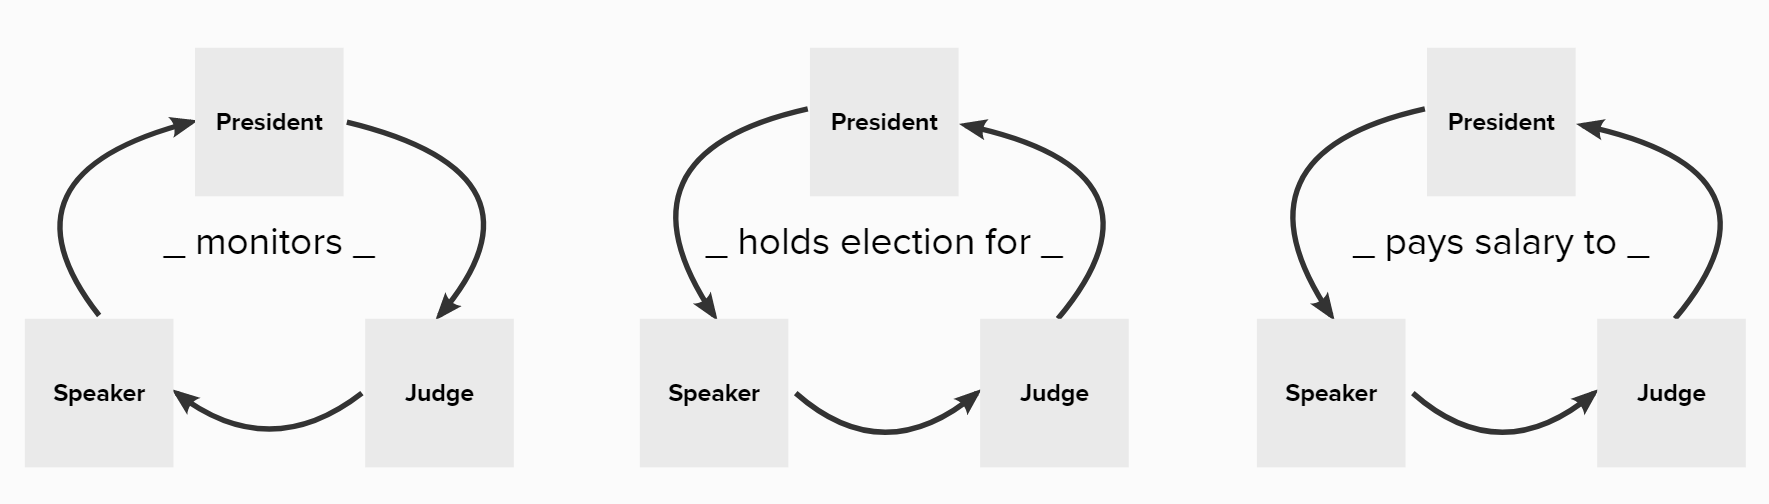
\includegraphics[scale=0.33]{05_iigo/images/role cycles.png}
\caption{Accountability cycle (left), the transfer-of-power cycle (middle) and salary cycle (right).}
\label{fig:cycles_in_IIGO}
\end{figure}


\subsection{Transfer-of-power}
\label{subsec:transfer-of-power}
\begin{enumerate}
    \item The Speaker conducts a vote for the election of the new Judge.
    \item The Judge conducts a vote for the election of the new President.
    \item The President conducts a vote for the election of the new Speaker.
\end{enumerate}
Refer to the Figure~ \ref{fig:cycles_in_IIGO} for further clarification about the transfer-of-power cycle.

\begin{rule_IIGO}
   The role $X$ has the \emph{obligation} to conduct a vote for the election of $Y$ at the end of the term (see Definition~\ref{def:term}) if and only if the role $X$ is accountable to the role $Y$. 
\end{rule_IIGO}.

\section{Budget and Salary}
\subsection{Budget}
%Actions associated with the IIGO have an associated cost that is defined as a configuration parameter. The institutional-power-enabled actions of  identified to require a "computational" component are:

Institutional-enabled-power actions in the IIGO have an associated cost with them. Some examples for such actions include:


%that is defined as a configuration parameter. The institutional-power-enabled actions of  identified to require a "computational" component are:


%We have defined the resource to be an endogenous one, hence any computation surrounding the distribution of the resource must use up some of that resource. 
\begin{itemize}
\item Calling any vote and computing the winner.
\item Declaring (e.g. \textit{announcing} the result of a vote).
\item Setting the amount of \emph{taxation} for each island.
\item Deciding the allocation distribution for each island.
\item Inspecting an island's action history.
\item Monitoring a role.
\end{itemize}

Since IIGO has been designed to act in the common good, IIGO-related costs will be directly withdrawn from the common pool. Since the common pool is considered a communal property of the archipelago, there are rules in place to limit how much each role is allowed to spend in order to perform its own institutional-power-enabled actions. This is the reason why defining the \emph{budget} and keeping it separate for each of the three IIGO roles.


As a role performs institutional-enabled-power actions, the corresponding cost associated with this action is subtracted from the role's budget. A budget of zero means that the role does not have the \emph{power} to perform any of its institutional-power-enabled actions. The removal of the budget rule from the rules in play means the role is allowed to perform as many such actions as it prefers to (as long as those actions are not governed by other rules). 



%As a role performs an endogenous-cost action, the corresponding cost associated with this action is subtracted from the role's budget. Thus, if as a result of an endogenous-cost action a role will be left with negative budget, it will have gone over the budget limit and will have broken the budget rule. A budget of zero means that the role is not allowed to perform any of its institutional-power-enabled actions associated an endogenous-cost. The removal of the budget rule from the rules in play means the role is allowed to perform as many such actions as it pleases (as long as those actions are not governed by other rules). 

The budget rule is also persistent across turns. This means that, assuming nothing else affects the budget, if a role has $100$ resources in its budget at each turn and spends only $10$ resources, this means that this very same role has $90$ resources in its budget at the next turn. On the other hand, islands can choose to increase the budget periodically every turn. This is governed by another budget extension rule.




%one turn and it spends 10, it has 90 resources in it's budget the next turn. 

Finally, it must be noted that the budget is inherently linked with the fact that whether obligations of a specific role can be undergone.
For example, during \emph{monitoring}, it should not be seen as a rule violation if a role has not acted on an obligation if it would go over the budget as a result. 

%This can also be seen as an added clause "... and the action is only permitted if they have the budget" to most rules which govern actions with an endogenous-cost.
%\begin{rule_IIGO}
    %The budget is increased by an amount $N$ every turn.
%\end{rule_IIGO}

%This rule means that, assuming nothing else affects the budget, if a budget is set to increase by 10 resources every turn and the budget is a 100 resources in turn one, the budget is 110 resources in turn 2. Setting this rule to 0 is equal to removing this rule and it means that the budget is never increased. 


\subsection{Salary}
\label{subsec:salary}
A salary is paid to each role in power as an incentive to act in a publicly approved way. %Hence, each role has the \emph{power} to pay a salary to another role following the salary cycle in Figure~\ref{fig:cycles_in_IIGO}.
\begin{rule_IIGO} \label{rule:salary}
   %Each role has the \emph{obligation} to pay the salary of amount $S$ to another if and only if the amount paid $S'$ is equal to $S$.
   Each role has the \emph{obligation} to pay the salary of amount $S$ to one another following the salary cycle in Figure~\ref{fig:cycles_in_IIGO}.
\end{rule_IIGO}

In Rule~\ref{rule:salary}, setting $S=0$ (through changing the active rules in place) means that roles do not have the permission to pay any salary. Removing the Rule~\ref{rule:salary} means that the roles may freely choose the amount $S$ for the salary payments.

\section{IIGO Session order}

\begin{enumerate}
    \item The Judge has the \emph{power} to check the history of actions to confirm whether the previously punished island(s) has/have obeyed the previous round's sanctions, meaning whether they contributed to the common pool accordingly in case of economic sanctions.
    %\begin{itemize}
      %  \item \emph{Suggested Rule:} In case of disobeying sanctions, the Judge is \emph{obliged} and \emph{permitted} to increase the severity of sanctions with respect to specific islands.
   % \end{itemize}
    \item The Judge has the \emph{power} to carry out \emph{inspections} on the history of actions of any island $X$ to check whether:
        \begin{enumerate}
        \item the reported resources of $X$ in the previous round match the real value of resources $X$ had in its private pool for the previous turn.
        \item the island $X$ has retrieved the right amount of the resources from the common pool, based on the \emph{allocation request} evaluated by the previous President.
            \begin{itemize}
            \item An example: In the previous round, the President has decided that the island $X$ can take $Y$ amount of resources from the common pool. If the Judge finds out that the island $X$ has taken an amount of $Y'$ such that $Y' > Y$, the Judge has the \emph{power} to invoke sanctions on the island $X$.
            
            %the Judge is \emph{obliged} and \emph{permitted} to sanction island $X$.
            \end{itemize}
        \end{enumerate}
    \item The Judge has the \emph{power} to invoke sanctions based on the outcome of the inspections.
    \item The President has the \emph{power} to decide to carry out a \emph{monitoring} on:
        \begin{enumerate}
        \item the sanctions imposed by the Judge.
        \end{enumerate}
    \item The islands may report the resources in their private pools to the President.
    \item The President has the \emph{power} to let each island know about the amount of \emph{taxation} they have to pay.
    \item The island has the \emph{power} to make an \emph{allocation request} to the President.
    \item The President has the \emph{power} decide on an allocation of resources and let each island know about the amount of resource allocation they are permitted to take from the common pool.
    \item The island has the \emph{power} to pick and to propose a rule to be voted on to the President.
    \item The President has the \emph{power} to choose a rule to be voted on from the received rule proposals.
    \item The Speaker has the \emph{power} to decide to carry out a \emph{monitoring} on: 
        \begin{enumerate}
        \item the resource allocation decided by the President.
        \item the rule proposed by the President.
        \end{enumerate}
    \item The Speaker has the \emph{power} to call a vote.
        \begin{enumerate}
        \item The islands vote in support of, or against, the rule (aye or nay) anonymously.
        \end{enumerate}
    \item The Speaker has the \emph{power} to announce a result of a vote to the islands and carries out the law change, if required (e.g. deleting/rejecting a rule if there is a majority nay vote).
    \item The Judge has the \emph{power} to decide to carry out \emph{monitoring} on:
        \begin{enumerate}
        \item the vote called by the Speaker.
        \item the Speaker announcing the result.
    \end{enumerate}
    \item The roles pay salary for one another following the accountability cycle in Figure~ \ref{fig:cycles_in_IIGO}.

\end{enumerate}



\section{Future Work}

\begin{itemize}
    \item \textbf{Diplomatic sanctions}: Although having the potential of being a good alternative for severer sanctions discussed in  Section~\ref{sec:sanctions}, diplomatic sanctions are \emph{not} implemented within the scope of the coursework. \\
    Suggested diplomatic sanctions include:
        \begin{itemize}
            \item Revoking an island's eligibility to vote and to be elected for a position.
            \item Revoking an island's eligibility to propose a rule/motion.
        \end{itemize}
    \item \textbf{Immutable rules}: Within the scope of the coursework, a subset of rules could have been categorised as immutable. This means that to change such immutable rules, the islands first need to vote to change their status to be \emph{mutable}, and consequently, hold another vote to change these mutable rules.
    %\item \textbf{Adding rules to the proposal list: } 
\end{itemize}

    \chapter{Inter-Island Governmental Organisation (IIGO)}


The role of IIGO is to maintain, update, and revise the rules concerning provision to managing the long-term collective risk dilemma (ltCRD). 

\begin{itemize}
    \item There will be 3 distinct branches in the IIGO: the \textbf{legislative branch}, \textbf{executive branch} and \textbf{judicial branch}\footnote{This is, as no surprise, inspired by the separation of powers in Western democracies.}.
    \item Each role is put in power according to the  transfer-of-power rules (see Section~\ref{subsec:transfer-of-power} for more detail).
    \item The head of the legislative branch is the Speaker, the head of the executive branch is the President, and the head of judicial branch is the Judge.
    \begin{itemize}
        \item  The Speaker, President and Judge are selected, through a democratic election, from the islands in the archipelago\footnote{This naming is inspired by the roles in the US Government.}.
        \item The resources gathered by the archipelago are endogenous, hence acting on the institutional powers granted to the Speaker, President or Judge costs resources. 
        \item For their duty, the President, the Speaker and the Judge receive a salary for each of their turns in office (see Section~\ref{subsec:salary} for more detail).
        \item The limit of the powers of the President, Speaker and Judge are defined in this chapter (e.g. the Speaker can only call one vote per turn).
 
    \end{itemize}
\end{itemize}

\subsection{IIGO Specific Definitions}
\begin{definition} \label{def:ballot}
    A \textbf{ballot} is related to each island's \textbf{power} to support or disagree with the rule specified in the vote called by the President and to vote in favour or against an island for a specific role (i.e. the President, Speaker, Judge) at each round of the game.
\end{definition}


%\begin{definition} \label{def:vote}
    %A \textbf{vote} is related to a role's (i.e. the President, Speaker, Judge) \textbf{power} to call a vote for a specific rule or an election.
%\end{definition}


\begin{definition} \label{def:tax}
    The \textbf{taxation} is related to the President's \textbf{power} to request a specific \underline{\textbf{minimum}} amount of contribution from each island to the common pool at each round of the game. 
\end{definition}

\begin{definition} \label{def:alloc_req}
    An \textbf{allocation request} is related to each island's \textbf{power} to request a specific amount of resource allocation from the President at each round of the game.
\end{definition}


\begin{definition} \label{def:rule_prop_list}
A \textbf{rule proposal list} is related to each island's \textbf{power} to propose a specific rule to be passed to the President at each round of the game.
\end{definition}

\begin{definition} \label{def:invst}
    An \textbf{investigation} is related to the Judge's \textbf{power} to acquire information to make a decision, followed by a calculation of the expected results and checking whether some specific rules have been obeyed, exclusively for the actions carried out by the \textbf{islands}. 
\end{definition}


An example of an \emph{investigation}: The President has permitted the island $X$ to take the amount of $Y$ resources from the common pool. Upon \emph{investigation} carried out by the Judge, it is revealed that the amount of resources taken out from the common pool by the island $X$ is, in fact, $Y'$ such that $Y' \neq Y$.


\begin{definition}
\textbf{Monitoring} is a government official's \textbf{power} to perform event recognition and to check whether some specific rules have been obeyed.
\end{definition}

An example of \emph{monitoring}: The Speaker has performed only the following action: \emph{counted the votes and calculated the result} for a rule. Upon \emph{monitoring} carried out by the President, it is noticed that the Speaker has not made any \emph{announcement}. Hence, the Speaker has not followed their obligation to \emph{announce} the result of any vote held.

See Section~\ref{sec:accountability} for more information about which roles can monitor which ones.


\begin{definition}
\textbf{Investigative-monitoring} is a government official's \textbf{power} to acquire the information used in acting on a governmental power followed by calculation of the expected results and checking whether some specific rules have been obeyed, exclusively for the actions carried out by a government official they are responsible for.
\end{definition}

An example of \emph{investigative-monitoring}: The Speaker has performed the following actions: \emph{counted the votes and calculated the result $R$} for a vote $V$ and \emph{announced} the result $R'$ for the vote $V$. Upon \emph{investigative-monitoring} carried out by the President, it is noticed that $R' \neq R$. Hence, the Speaker has modified the announced result.


\begin{definition}
The \textbf{sanction} is related to the Judge's \emph{power} to punish non-compliant islands when their disobedience is confirmed through investigations at a specific turn.
\end{definition}


\begin{definition}
The (judicial) \textbf{pardon} is related to the Judge's \emph{power} to forgive a non-compliant island at a specific turn.
\end{definition}

\begin{definition}
The \textbf{budget} is the maximum amount of resources a role is permitted to spend from the common pool as it performs its own institutional-power-enabled actions at a specific turn.
\end{definition}


\begin{definition}
The \textbf{salary} is the amount of resources a role is to be given from the common pool as a reward for performing its institutional-power-enabled actions at a specific turn.
\end{definition}

\begin{definition} \label{def:term}
A \textbf{term} is the number of turns an island is \emph{permitted} to hold a role, and after which the responsible role (indicated in the transfer-of-power cycle in Figure~\ref{fig:cycles_in_IIGO}) is \emph{obliged} to initiate transfer-of-power.
\end{definition}

\subsection{\emph{Power}, \emph{Permission} and \emph{Obligation} Distinction}
In the rest of the specifications, we will be specifically using the following three terms to define the actions and responsibilities carried out by the Speaker, President, Judge (see Figure~ \ref{fig:per_obl_sets}):
\begin{itemize}
    \item Power
    \item Permission
    \item Obligation
\end{itemize}



\begin{figure}[H] 
\centering
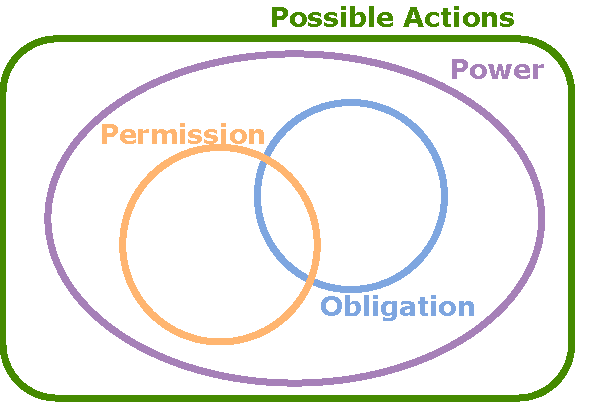
\includegraphics[width=0.6\textwidth]{05_iigo/images/SOMAS_per_obl.pdf}
\caption{Relationship between \emph{power}, \emph{permission} and \emph{obligation}.}
\label{fig:per_obl_sets}
\end{figure} 


For example, the Judge has the \emph{power} to carry out investigations at an IIGO session. There are no rules specifying which specific islands the Judge should investigate. Therefore, the Judge has the \emph{permission} to investigate any `alive' islands during a session. However, the Judge is \emph{obliged} to make at least some number of investigations each turn.



\section{Executive Branch}
\label{sec:executive}
The executive branch is responsible for \textbf{carrying out the law}.
\begin{itemize}
       
    \item The President has the \emph{power} to: 
    \begin{itemize}
        
        \item Select a rule for voting $R^{*}$ to be passed to the Speaker.
        \begin{rule_IIGO}
            The President has the \emph{obligation} to \emph{select} a rule $R^{*}$ if the \emph{rule proposal list} has at least one proposed rule in it.
        \end{rule_IIGO}
        \begin{rule_IIGO}
            The President has the \emph{permission} to \emph{select} a rule $R^{*}$ if and only if $R^{*} \in S$, where $S$ is the \emph{rule proposal list}.
        \end{rule_IIGO}
        
        \item Decide the amount of individual \emph{taxation} (i.e. a specific \emph{minimum} amount of contribution to the common pool for each island) for the current turn.
        
        \begin{itemize}
            \item The President is given the self-reported resource amounts held by each island to assist in this decision.
            %\item Suggested Rule: For any island that has chosen to not report it's resources, the President has the \emph{obligation} to set them an individual tax amount T.
        \end{itemize}
        
        \item Decide the allocation of resources distributed from the common pool to the islands (i.e. a specific \emph{maximum} amount an island is permitted to take from the common pool).
        
        \begin{itemize}
            \item The President is given the \emph{allocation requests} made by each island.
            %\item \emph{}{Suggested Rule:} The President has an obligation to prioritise islands in critical condition.
        \end{itemize}
    \end{itemize}
\end{itemize}



\section{Legislative Branch}
\label{sec:legislative}
The legislative branch is responsible for \textbf{making the law}.
\begin{itemize}

    \item The Speaker has the \emph{power} to:
    \begin{itemize}
        
        \item Call a vote $V$ for a rule $R$.
        \begin{rule_IIGO}
            The Speaker has the \emph{obligation} to \emph{call} a vote $V$ if and only if the President has \emph{selected} a rule $R$ to be voted on.
        \end {rule_IIGO}
        \begin{rule_IIGO}
            The Speaker has the \emph{permission} to \emph{call} a vote $V$ for a rule $R$ if and only if the rule $R = R^{*}$, where $R^{*}$ is the rule \emph{selected} by the President.
        \end {rule_IIGO}
            
        \item Choose which islands are participating in the vote $V$.
       % \footnote{This is our sequential implementation alternative for the power to close the ballot box.}.
        \begin{rule_IIGO}
            The Speaker has the \emph{obligation} to ask for a vote from all alive islands.
        \end {rule_IIGO}
            
        \item Declare the result $C$ of a vote $V$. 
        \begin{rule_IIGO}
            The Speaker has the \emph{obligation} to \emph{declare the result} $C$ for a vote $V$ if and only if the vote V has been \emph{called}.
        \end {rule_IIGO}
        \begin{rule_IIGO}
            The Speaker has the \emph{permission} to \emph{declare the result} $C$ for a vote $V$ if $C = C^{*}$, where $C^{*}$ is the result produced by \emph{calling} the vote $V$.
        \end {rule_IIGO}
        \begin{itemize}
            \item This step is what enables a rule to be \emph{active}.
        \end{itemize}
    \end{itemize}
\end{itemize}




\section{Judicial Branch}
\label{sec:judicial}

The judicial branch is responsible for \textbf{evaluating the law}.
\begin{itemize}
    \item The Judge has the \emph{power} to:
    \begin{itemize}
        \item Perform a number of \emph{inspections}\footnote{An \emph{inspection} \textbf{costs} an expense of resources (See Definition~\ref{def:invst} for more detail).} $I$ and produce a compliance outcome $\mathbb{O}^{*}$\footnote{Note that the compliance outcome $\mathbb{O}^{*}$ considered is a boolean.}.
        %(true: the island has been compliant with the rules in play, false: the island has not been compliant with the rules in play)
        %\begin{itemize}
           % \item For example, to check if the event outcome is \emph{concurrent}\footnote{Again, what is defined as "concurrent"? A clear definition is needed.} with the rules.
        %\end{itemize}
        \begin{rule_IIGO}
            The Judge has the \emph{obligation} to make at least $N$ investigations at each turn.
        \end{rule_IIGO}
        \item Declare the outcome $\mathbb{O}$ of an inspection $I$ to all islands\footnote{This act of broadcasting is especially important for islands to form an opinion about the sanctioned islands accordingly.}.
        \begin{rule_IIGO}
            The Judge has the \emph{obligation} to declare the outcome $\mathbb{O}$ of an inspection $I$ if and only if the inspection $I$ has been performed.
        \end{rule_IIGO}
        \begin{rule_IIGO}
            The Judge has the \emph{permission} to declare the outcome $\mathbb{O}$ of an inspection $I$ if $\mathbb{O} = \mathbb{O}^{*}$, where $\mathbb{O}^{*}$ is the outcome of the inspection $I$.
        \end{rule_IIGO}
        %\item Initiate the removal of the \texttt{President}.
        %\begin{itemize}
            %\item A good Judge would be especially vigilant during \emph{power transfer} regarding the \emph{President} position (see Section~\ref{leg_const} for more detail).
        %\end{itemize}
        \item Invoke economic \textbf{sanctions} (see Section~\ref{sec:sanctions} for more detail).
        \begin{rule_IIGO}
            The Judge has the \emph{obligation} to invoke a sanction $S$ for an island $X$ if and only if an investigation $I$ has an outcome $\mathbb{O}^{*}$ indicating non-compliance, and $I$ is an investigation of an action taken by island $X$.
        \end{rule_IIGO}
        \item Invoke even more severe sanctions in the case of further disobedience to previous sanction(s).
        \begin{rule_IIGO}
            The Judge has the \emph{permission} to invoke a severer sanction $S'$ for an island $X$ if the island $X$ has not fulfilled the requirements of the previous sanction $S$.
        \end{rule_IIGO}
        \item Pardon the islands which are currently sanctioned.
        \begin{rule_IIGO}
            The Judge has the \emph{permission} to revoke any sanction $S$ of an island $X$ at a specific turn.
        \end{rule_IIGO}
    \end{itemize}
\end{itemize}
%(e.g. a new rule that falls under a "sanction" category \hl{[I'm not sure about this being a `new rule` [Ezgi]]}

\subsection{Sanctions}
\label{sec:sanctions}
All sanctions are of economic nature which include:
        \begin{itemize}
            %\item Revoking an island's access to the common pool.
            \item Enforcing an island to contribute a specific amount of resources to the common pool.
            \begin{itemize}
                \item This does not mean that the Judge has the \emph{power} to take resources from an island in order to put them to the common pool -- the island itself is expected to carry out this implication imposed by the sanction itself, otherwise further punishment can be induced by the Judge.
                \item Similarly, \emph{opinion formulation} will follow accordingly whether the island(s) is/are following the implications imposed by the sanction(s).
            \end{itemize}
        
    \end{itemize}
    Sanctions are the associated penalty that comes with an island breaking a specific rule. The Judge is in full control of the penalties associated with breaking any rules. Once the Judge has specified the score of the penalty associated with each time an island breaks a rule, the cumulative penalties accumulated by the island are then used to determine which \textbf{sanction tier} that each island falls into. The score threshold to determine the boundaries of the sanction tiers are set by the Judge. At each turn of the game, each island is told whether they are being sanctioned, and if so, which \textbf{sanction tier} that they are currently in. The \textbf{sanction tiers} of the non-compliant islands are also broadcasted to the other islands in the archipelago. To summarise, the sanctioning process follows these steps:
    
    
    
    %Sanctions are based on an island breaking a rule. Each rule must therefore have an associated penalty. By default, we set these penalties such that they add $1$ to the total sanction score for each island. However, we allow the judge to override this scoring, the judge is able to set their own scores for any particular rule as they desire. This custom scoring is then used when an island breaks a particular rule. By looking at events that occurred in the last turn, and using the customised scoring we provide the holder of the judge role with full control of the penalties for breaking any rules.
    
    





%we then use the cumulative penalties accumulated by each island to determine which Sanction Tier they fall into. The score threshold's required to fall into these sanction tiers is set by the judge and is checked for monotonicity. Each island is told whether they are being sanctioned, and is so what tier they are in. We also tell other islands about which sanction tiers other islands have fallen into. 

    \begin{enumerate}
        \item The Judge has the \emph{power} to set custom penalties associated with breaking any rules.
        \item The Judge is given a list of all events that occurred in the previous turn.
        \item The Judge has the \emph{power} to check whether any, or all of these previous events, involve the islands in the archipelago breaking any rules.
        \item Each of the transgressions is scored using the Judge's custom penalties if the Judge has set them. Otherwise, a score of $1$ is given each time a rule is broken.
        \item The Judge has the \emph{power} to revise the sanction thresholds.
        \item Using the latest sanction thresholds available, each island is assigned to a sanction tier based on the sanction score that it has received.
        \item These sanction tiers are broadcasted to all of the islands in the archipelago.
        \item The Judge then uses sanctions rules in place to calculate the specific amount of resources that each non-compliant island has in order to determine how much it should contribute to the common pool, based on the sanction tier that it is in.
    \end{enumerate}



\section{Constitutional Rights and Obligations in the Archipelago}
\label{sec:const_rights_obl_archi}
Each island has the \emph{power} to:
\begin{itemize}
\item make an \emph{allocation request} (see Definition~\ref{def:alloc_req}) to the President for a specific amount to be allocated to them.
\item report the number of resources it is in possession of to the President.
\begin{rule_IIGO}
    Each island has the \emph{obligation} to report the number of resources it is in possession of to the President.
\end{rule_IIGO}
\begin{rule_IIGO}
    Each island has the \emph{permission} to report the number of resources $R'$ if and only if $R' = R$, where R is the number of resources the island is in possession of.
\end{rule_IIGO}
\item take resources from the common pool.


\begin{rule_IIGO}
    Each island has the \emph{permission} to take at maximum $N$ resources, where $N$ is the specific allocation made by the President to that island\footnote{If no such allocation is made, the island is \emph{permitted} to take any amount of resources.}.
\end{rule_IIGO}
\item contribute resources to the common pool.
\begin{rule_IIGO}
    Each island has the \emph{obligation} to contribute to the common pool an amount greater or equal to that of the individual tax set by the President.
\end{rule_IIGO}
                %The President is in
                %(unless there is a rule in place that dictates how Speaker is to allocate resources).
\item add a rule to the \emph{rule proposal list} (see Definition~\ref{def:rule_prop_list}) at the start of each turn.
        %\begin{itemize}
            %\item The game specification includes how many rules an island can propose each turn.
        %\end{itemize}
        %\item vote  for rules in the Legislative Branch and vote for their favourite islands in elections
\item participate in the legislative branch of the government by casting ballots in votes called by the Speaker
\item vote for an island to be elected for a specific role (e.g. the President, Judge, Speaker) during the elections\footnote{This will be assumed to be true \underline{unless stated otherwise}. %Note that \textbf{diplomatic sanctions} can disable this power of a specific island (see Section~\ref{jud_const}).}.
        }.
\end{itemize}
\section{Accountability Cycle}
\label{sec:accountability}


To ensure that the government avoids corruption and abuse of power, each branch is accountable to another. The President is accountable to the Speaker, the Speaker is accountable to the Judge, and the Judge is accountable to the President (see Figure~ \ref{fig:cycles_in_IIGO}). This accountability cycle is enacted through \emph{monitoring} actions\footnote{Note that the terms \textbf{monitoring} and \textbf{investigation} have similar but quite different meanings in the IIGO context.}. 

The powers related to the accountability cycle and transfer-of-power for each role can be summarized as the following: 
\begin{itemize}
    \item The Speaker has the \emph{power} to: 
    \begin{itemize}
        \item monitor the President.
        \item announce the result of this monitoring.
        \item initiate the transfer-of-power for the Judge.
    \end{itemize}
    \item The President has the \emph{power} to: 
    \begin{itemize}
        \item monitor the Judge.
        \item announce the result of this monitoring.
        \item initiate the transfer-of-power for the Speaker.
    \end{itemize}
    \item The Judge has the \emph{power} to: 
    \begin{itemize}
        \item  monitor the Speaker.
        \item announce the result of this monitoring.
        \item initiate the transfer-of-power for the President.
    \end{itemize}
\end{itemize}

%Unlike investigations performed by the Judge, who performs investigations on island actions in the following turn, each role is given the opportunity to check up on the actions of the role it is responsible for immediately after they have been performed. In this sense, the President can monitor (includes investigative-monitoring) the powers (calling a vote and announcing the result) acted on by the Speaker immediately after the Speaker's announcement (or lack there of). The government officials hold a lot of power so this is to ensure that any wrong-doing is determined as quickly as possible. For this project we are only pursuing one degree of monitoring, that is, the powers relating to the accountability cycle will not be monitored themselves. We assume that agents will act in the interest of themselves and keeping all the islands alive is beneficial to everyone. Hence, while the agents might be inclined to break rules in order to benefit themselves, anyone else breaking the rules is seen as undesirable under the assumption that the system in place is there to benefit all. 


Through the proposed accountability cycle, each role is given the opportunity to check up on the actions of the role it is accountable for immediately after they have been performed. It is clear that the IIGO roles (i.e. the President, Speaker and Judge) hold a considerable amount of \emph{power} in their hands. The accountability cycle is designed to address the possible abuses of this power. With monitoring, any wrong-doing in the IGO is determined as quickly as possible and the role in question can be replaced. 

Within the scope of the coursework, we decided to pursue only \emph{one degree of monitoring}, meaning that the powers relating to the accountability cycle will not be monitored themselves. We assume that agents will act in the interest of all the islands in the archipelago. Hence, while the agents might be inclined to break the rules to benefit in some form, it is assumed that the others will negatively see any non-compliant islands based on the assumption that the proposed IIGO system is in place to maintain the welfare of all the islands.

Let role $X$ be accountable to the role $Y$, which is accountable to the role $Z$. Then:
\begin{rule_IIGO}
$Y$ has the \emph{obligation} to declare the outcome of the monitoring result $M$ associated with the action $A$ undertaken by $X$ if and only if $Y$ has monitored the action $A$ performed by $X$. 
\end{rule_IIGO}
\begin{rule_IIGO}
$Y$ has the \emph{permission} to declare the monitoring result $M$ associated with the action $A$ undertaken by $X$ if and only if $M = M^{*}$, where $M^{*}$ is the outcome of \emph{monitoring} action $A$ performed by $X$\footnote{These constitutional rules should be available to the agents to check their decision against. However, due to having only one degree of accountability cycle in place, these rules are not enforced through any sanctions (i.e. breaking these rules has no consequences as they only deem to be an \emph{agreement} among the roles).}.
\end{rule_IIGO}


\begin{figure}[!htb]
\centering
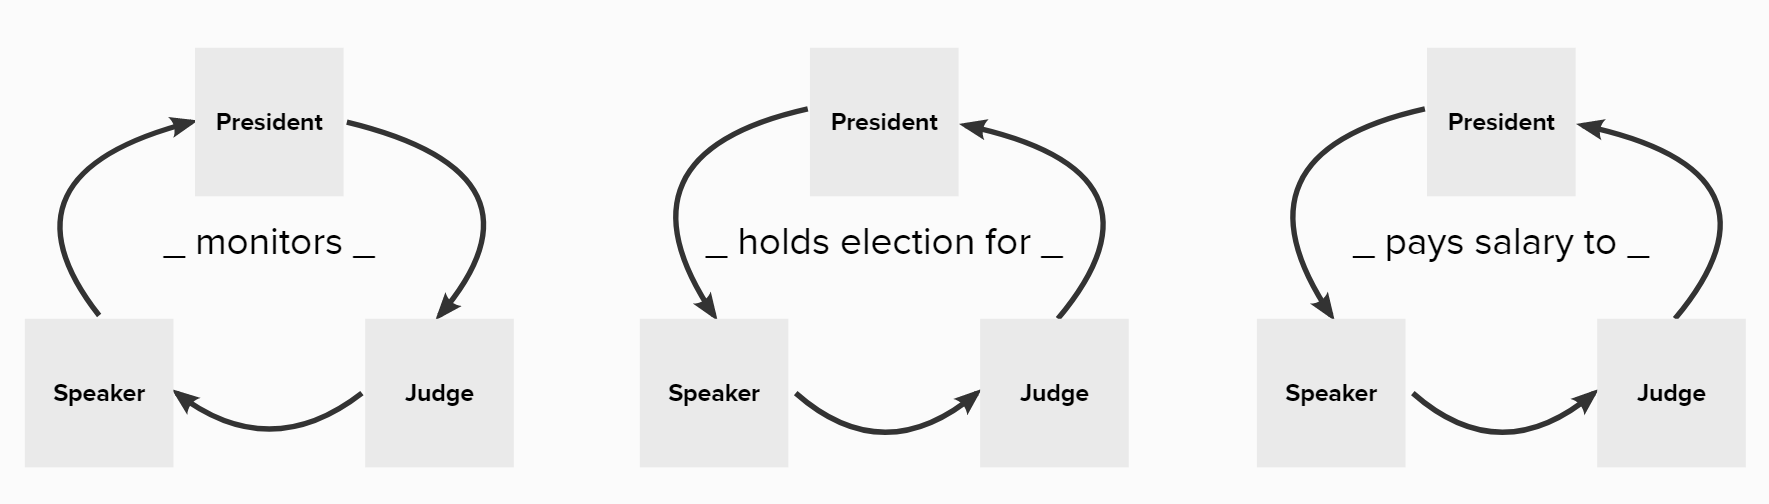
\includegraphics[scale=0.33]{05_iigo/images/role cycles.png}
\caption{Accountability cycle (left), the transfer-of-power cycle (middle) and salary cycle (right).}
\label{fig:cycles_in_IIGO}
\end{figure}


\subsection{Transfer-of-power}
\label{subsec:transfer-of-power}
\begin{enumerate}
    \item The Speaker conducts a vote for the election of the new Judge.
    \item The Judge conducts a vote for the election of the new President.
    \item The President conducts a vote for the election of the new Speaker.
\end{enumerate}
Refer to the Figure~ \ref{fig:cycles_in_IIGO} for further clarification about the transfer-of-power cycle.

\begin{rule_IIGO}
   The role $X$ has the \emph{obligation} to conduct a vote for the election of $Y$ at the end of the term (see Definition~\ref{def:term}) if and only if the role $X$ is accountable to the role $Y$. 
\end{rule_IIGO}.

\section{Budget and Salary}
\subsection{Budget}
%Actions associated with the IIGO have an associated cost that is defined as a configuration parameter. The institutional-power-enabled actions of  identified to require a "computational" component are:

Institutional-enabled-power actions in the IIGO have an associated cost with them. Some examples for such actions include:


%that is defined as a configuration parameter. The institutional-power-enabled actions of  identified to require a "computational" component are:


%We have defined the resource to be an endogenous one, hence any computation surrounding the distribution of the resource must use up some of that resource. 
\begin{itemize}
\item Calling any vote and computing the winner.
\item Declaring (e.g. \textit{announcing} the result of a vote).
\item Setting the amount of \emph{taxation} for each island.
\item Deciding the allocation distribution for each island.
\item Inspecting an island's action history.
\item Monitoring a role.
\end{itemize}

Since IIGO has been designed to act in the common good, IIGO-related costs will be directly withdrawn from the common pool. Since the common pool is considered a communal property of the archipelago, there are rules in place to limit how much each role is allowed to spend in order to perform its own institutional-power-enabled actions. This is the reason why defining the \emph{budget} and keeping it separate for each of the three IIGO roles.


As a role performs institutional-enabled-power actions, the corresponding cost associated with this action is subtracted from the role's budget. A budget of zero means that the role does not have the \emph{power} to perform any of its institutional-power-enabled actions. The removal of the budget rule from the rules in play means the role is allowed to perform as many such actions as it prefers to (as long as those actions are not governed by other rules). 



%As a role performs an endogenous-cost action, the corresponding cost associated with this action is subtracted from the role's budget. Thus, if as a result of an endogenous-cost action a role will be left with negative budget, it will have gone over the budget limit and will have broken the budget rule. A budget of zero means that the role is not allowed to perform any of its institutional-power-enabled actions associated an endogenous-cost. The removal of the budget rule from the rules in play means the role is allowed to perform as many such actions as it pleases (as long as those actions are not governed by other rules). 

The budget rule is also persistent across turns. This means that, assuming nothing else affects the budget, if a role has $100$ resources in its budget at each turn and spends only $10$ resources, this means that this very same role has $90$ resources in its budget at the next turn. On the other hand, islands can choose to increase the budget periodically every turn. This is governed by another budget extension rule.




%one turn and it spends 10, it has 90 resources in it's budget the next turn. 

Finally, it must be noted that the budget is inherently linked with the fact that whether obligations of a specific role can be undergone.
For example, during \emph{monitoring}, it should not be seen as a rule violation if a role has not acted on an obligation if it would go over the budget as a result. 

%This can also be seen as an added clause "... and the action is only permitted if they have the budget" to most rules which govern actions with an endogenous-cost.
%\begin{rule_IIGO}
    %The budget is increased by an amount $N$ every turn.
%\end{rule_IIGO}

%This rule means that, assuming nothing else affects the budget, if a budget is set to increase by 10 resources every turn and the budget is a 100 resources in turn one, the budget is 110 resources in turn 2. Setting this rule to 0 is equal to removing this rule and it means that the budget is never increased. 


\subsection{Salary}
\label{subsec:salary}
A salary is paid to each role in power as an incentive to act in a publicly approved way. %Hence, each role has the \emph{power} to pay a salary to another role following the salary cycle in Figure~\ref{fig:cycles_in_IIGO}.
\begin{rule_IIGO} \label{rule:salary}
   %Each role has the \emph{obligation} to pay the salary of amount $S$ to another if and only if the amount paid $S'$ is equal to $S$.
   Each role has the \emph{obligation} to pay the salary of amount $S$ to one another following the salary cycle in Figure~\ref{fig:cycles_in_IIGO}.
\end{rule_IIGO}

In Rule~\ref{rule:salary}, setting $S=0$ (through changing the active rules in place) means that roles do not have the permission to pay any salary. Removing the Rule~\ref{rule:salary} means that the roles may freely choose the amount $S$ for the salary payments.

\section{IIGO Session order}

\begin{enumerate}
    \item The Judge has the \emph{power} to check the history of actions to confirm whether the previously punished island(s) has/have obeyed the previous round's sanctions, meaning whether they contributed to the common pool accordingly in case of economic sanctions.
    %\begin{itemize}
      %  \item \emph{Suggested Rule:} In case of disobeying sanctions, the Judge is \emph{obliged} and \emph{permitted} to increase the severity of sanctions with respect to specific islands.
   % \end{itemize}
    \item The Judge has the \emph{power} to carry out \emph{inspections} on the history of actions of any island $X$ to check whether:
        \begin{enumerate}
        \item the reported resources of $X$ in the previous round match the real value of resources $X$ had in its private pool for the previous turn.
        \item the island $X$ has retrieved the right amount of the resources from the common pool, based on the \emph{allocation request} evaluated by the previous President.
            \begin{itemize}
            \item An example: In the previous round, the President has decided that the island $X$ can take $Y$ amount of resources from the common pool. If the Judge finds out that the island $X$ has taken an amount of $Y'$ such that $Y' > Y$, the Judge has the \emph{power} to invoke sanctions on the island $X$.
            
            %the Judge is \emph{obliged} and \emph{permitted} to sanction island $X$.
            \end{itemize}
        \end{enumerate}
    \item The Judge has the \emph{power} to invoke sanctions based on the outcome of the inspections.
    \item The President has the \emph{power} to decide to carry out a \emph{monitoring} on:
        \begin{enumerate}
        \item the sanctions imposed by the Judge.
        \end{enumerate}
    \item The islands may report the resources in their private pools to the President.
    \item The President has the \emph{power} to let each island know about the amount of \emph{taxation} they have to pay.
    \item The island has the \emph{power} to make an \emph{allocation request} to the President.
    \item The President has the \emph{power} decide on an allocation of resources and let each island know about the amount of resource allocation they are permitted to take from the common pool.
    \item The island has the \emph{power} to pick and to propose a rule to be voted on to the President.
    \item The President has the \emph{power} to choose a rule to be voted on from the received rule proposals.
    \item The Speaker has the \emph{power} to decide to carry out a \emph{monitoring} on: 
        \begin{enumerate}
        \item the resource allocation decided by the President.
        \item the rule proposed by the President.
        \end{enumerate}
    \item The Speaker has the \emph{power} to call a vote.
        \begin{enumerate}
        \item The islands vote in support of, or against, the rule (aye or nay) anonymously.
        \end{enumerate}
    \item The Speaker has the \emph{power} to announce a result of a vote to the islands and carries out the law change, if required (e.g. deleting/rejecting a rule if there is a majority nay vote).
    \item The Judge has the \emph{power} to decide to carry out \emph{monitoring} on:
        \begin{enumerate}
        \item the vote called by the Speaker.
        \item the Speaker announcing the result.
    \end{enumerate}
    \item The roles pay salary for one another following the accountability cycle in Figure~ \ref{fig:cycles_in_IIGO}.

\end{enumerate}



\section{Future Work}

\begin{itemize}
    \item \textbf{Diplomatic sanctions}: Although having the potential of being a good alternative for severer sanctions discussed in  Section~\ref{sec:sanctions}, diplomatic sanctions are \emph{not} implemented within the scope of the coursework. \\
    Suggested diplomatic sanctions include:
        \begin{itemize}
            \item Revoking an island's eligibility to vote and to be elected for a position.
            \item Revoking an island's eligibility to propose a rule/motion.
        \end{itemize}
    \item \textbf{Immutable rules}: Within the scope of the coursework, a subset of rules could have been categorised as immutable. This means that to change such immutable rules, the islands first need to vote to change their status to be \emph{mutable}, and consequently, hold another vote to change these mutable rules.
    %\item \textbf{Adding rules to the proposal list: } 
\end{itemize}

    \chapter{Inter-Island Governmental Organisation (IIGO)}


The role of IIGO is to maintain, update, and revise the rules concerning provision to managing the long-term collective risk dilemma (ltCRD). 

\begin{itemize}
    \item There will be 3 distinct branches in the IIGO: the \textbf{legislative branch}, \textbf{executive branch} and \textbf{judicial branch}\footnote{This is, as no surprise, inspired by the separation of powers in Western democracies.}.
    \item Each role is put in power according to the  transfer-of-power rules (see Section~\ref{subsec:transfer-of-power} for more detail).
    \item The head of the legislative branch is the Speaker, the head of the executive branch is the President, and the head of judicial branch is the Judge.
    \begin{itemize}
        \item  The Speaker, President and Judge are selected, through a democratic election, from the islands in the archipelago\footnote{This naming is inspired by the roles in the US Government.}.
        \item The resources gathered by the archipelago are endogenous, hence acting on the institutional powers granted to the Speaker, President or Judge costs resources. 
        \item For their duty, the President, the Speaker and the Judge receive a salary for each of their turns in office (see Section~\ref{subsec:salary} for more detail).
        \item The limit of the powers of the President, Speaker and Judge are defined in this chapter (e.g. the Speaker can only call one vote per turn).
 
    \end{itemize}
\end{itemize}

\subsection{IIGO Specific Definitions}
\begin{definition} \label{def:ballot}
    A \textbf{ballot} is related to each island's \textbf{power} to support or disagree with the rule specified in the vote called by the President and to vote in favour or against an island for a specific role (i.e. the President, Speaker, Judge) at each round of the game.
\end{definition}


%\begin{definition} \label{def:vote}
    %A \textbf{vote} is related to a role's (i.e. the President, Speaker, Judge) \textbf{power} to call a vote for a specific rule or an election.
%\end{definition}


\begin{definition} \label{def:tax}
    The \textbf{taxation} is related to the President's \textbf{power} to request a specific \underline{\textbf{minimum}} amount of contribution from each island to the common pool at each round of the game. 
\end{definition}

\begin{definition} \label{def:alloc_req}
    An \textbf{allocation request} is related to each island's \textbf{power} to request a specific amount of resource allocation from the President at each round of the game.
\end{definition}


\begin{definition} \label{def:rule_prop_list}
A \textbf{rule proposal list} is related to each island's \textbf{power} to propose a specific rule to be passed to the President at each round of the game.
\end{definition}

\begin{definition} \label{def:invst}
    An \textbf{investigation} is related to the Judge's \textbf{power} to acquire information to make a decision, followed by a calculation of the expected results and checking whether some specific rules have been obeyed, exclusively for the actions carried out by the \textbf{islands}. 
\end{definition}


An example of an \emph{investigation}: The President has permitted the island $X$ to take the amount of $Y$ resources from the common pool. Upon \emph{investigation} carried out by the Judge, it is revealed that the amount of resources taken out from the common pool by the island $X$ is, in fact, $Y'$ such that $Y' \neq Y$.


\begin{definition}
\textbf{Monitoring} is a government official's \textbf{power} to perform event recognition and to check whether some specific rules have been obeyed.
\end{definition}

An example of \emph{monitoring}: The Speaker has performed only the following action: \emph{counted the votes and calculated the result} for a rule. Upon \emph{monitoring} carried out by the President, it is noticed that the Speaker has not made any \emph{announcement}. Hence, the Speaker has not followed their obligation to \emph{announce} the result of any vote held.

See Section~\ref{sec:accountability} for more information about which roles can monitor which ones.


\begin{definition}
\textbf{Investigative-monitoring} is a government official's \textbf{power} to acquire the information used in acting on a governmental power followed by calculation of the expected results and checking whether some specific rules have been obeyed, exclusively for the actions carried out by a government official they are responsible for.
\end{definition}

An example of \emph{investigative-monitoring}: The Speaker has performed the following actions: \emph{counted the votes and calculated the result $R$} for a vote $V$ and \emph{announced} the result $R'$ for the vote $V$. Upon \emph{investigative-monitoring} carried out by the President, it is noticed that $R' \neq R$. Hence, the Speaker has modified the announced result.


\begin{definition}
The \textbf{sanction} is related to the Judge's \emph{power} to punish non-compliant islands when their disobedience is confirmed through investigations at a specific turn.
\end{definition}


\begin{definition}
The (judicial) \textbf{pardon} is related to the Judge's \emph{power} to forgive a non-compliant island at a specific turn.
\end{definition}

\begin{definition}
The \textbf{budget} is the maximum amount of resources a role is permitted to spend from the common pool as it performs its own institutional-power-enabled actions at a specific turn.
\end{definition}


\begin{definition}
The \textbf{salary} is the amount of resources a role is to be given from the common pool as a reward for performing its institutional-power-enabled actions at a specific turn.
\end{definition}

\begin{definition} \label{def:term}
A \textbf{term} is the number of turns an island is \emph{permitted} to hold a role, and after which the responsible role (indicated in the transfer-of-power cycle in Figure~\ref{fig:cycles_in_IIGO}) is \emph{obliged} to initiate transfer-of-power.
\end{definition}

\subsection{\emph{Power}, \emph{Permission} and \emph{Obligation} Distinction}
In the rest of the specifications, we will be specifically using the following three terms to define the actions and responsibilities carried out by the Speaker, President, Judge (see Figure~ \ref{fig:per_obl_sets}):
\begin{itemize}
    \item Power
    \item Permission
    \item Obligation
\end{itemize}



\begin{figure}[H] 
\centering
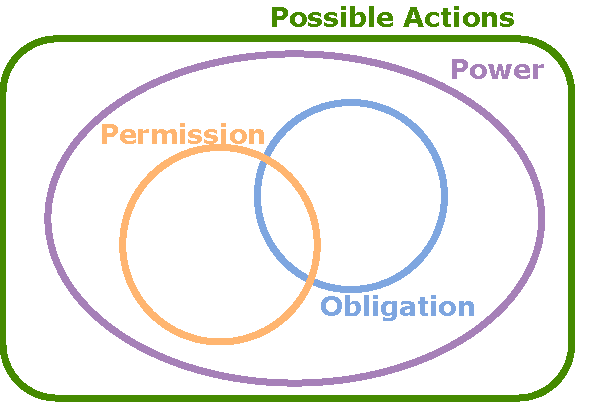
\includegraphics[width=0.6\textwidth]{05_iigo/images/SOMAS_per_obl.pdf}
\caption{Relationship between \emph{power}, \emph{permission} and \emph{obligation}.}
\label{fig:per_obl_sets}
\end{figure} 


For example, the Judge has the \emph{power} to carry out investigations at an IIGO session. There are no rules specifying which specific islands the Judge should investigate. Therefore, the Judge has the \emph{permission} to investigate any `alive' islands during a session. However, the Judge is \emph{obliged} to make at least some number of investigations each turn.



\section{Executive Branch}
\label{sec:executive}
The executive branch is responsible for \textbf{carrying out the law}.
\begin{itemize}
       
    \item The President has the \emph{power} to: 
    \begin{itemize}
        
        \item Select a rule for voting $R^{*}$ to be passed to the Speaker.
        \begin{rule_IIGO}
            The President has the \emph{obligation} to \emph{select} a rule $R^{*}$ if the \emph{rule proposal list} has at least one proposed rule in it.
        \end{rule_IIGO}
        \begin{rule_IIGO}
            The President has the \emph{permission} to \emph{select} a rule $R^{*}$ if and only if $R^{*} \in S$, where $S$ is the \emph{rule proposal list}.
        \end{rule_IIGO}
        
        \item Decide the amount of individual \emph{taxation} (i.e. a specific \emph{minimum} amount of contribution to the common pool for each island) for the current turn.
        
        \begin{itemize}
            \item The President is given the self-reported resource amounts held by each island to assist in this decision.
            %\item Suggested Rule: For any island that has chosen to not report it's resources, the President has the \emph{obligation} to set them an individual tax amount T.
        \end{itemize}
        
        \item Decide the allocation of resources distributed from the common pool to the islands (i.e. a specific \emph{maximum} amount an island is permitted to take from the common pool).
        
        \begin{itemize}
            \item The President is given the \emph{allocation requests} made by each island.
            %\item \emph{}{Suggested Rule:} The President has an obligation to prioritise islands in critical condition.
        \end{itemize}
    \end{itemize}
\end{itemize}



\section{Legislative Branch}
\label{sec:legislative}
The legislative branch is responsible for \textbf{making the law}.
\begin{itemize}

    \item The Speaker has the \emph{power} to:
    \begin{itemize}
        
        \item Call a vote $V$ for a rule $R$.
        \begin{rule_IIGO}
            The Speaker has the \emph{obligation} to \emph{call} a vote $V$ if and only if the President has \emph{selected} a rule $R$ to be voted on.
        \end {rule_IIGO}
        \begin{rule_IIGO}
            The Speaker has the \emph{permission} to \emph{call} a vote $V$ for a rule $R$ if and only if the rule $R = R^{*}$, where $R^{*}$ is the rule \emph{selected} by the President.
        \end {rule_IIGO}
            
        \item Choose which islands are participating in the vote $V$.
       % \footnote{This is our sequential implementation alternative for the power to close the ballot box.}.
        \begin{rule_IIGO}
            The Speaker has the \emph{obligation} to ask for a vote from all alive islands.
        \end {rule_IIGO}
            
        \item Declare the result $C$ of a vote $V$. 
        \begin{rule_IIGO}
            The Speaker has the \emph{obligation} to \emph{declare the result} $C$ for a vote $V$ if and only if the vote V has been \emph{called}.
        \end {rule_IIGO}
        \begin{rule_IIGO}
            The Speaker has the \emph{permission} to \emph{declare the result} $C$ for a vote $V$ if $C = C^{*}$, where $C^{*}$ is the result produced by \emph{calling} the vote $V$.
        \end {rule_IIGO}
        \begin{itemize}
            \item This step is what enables a rule to be \emph{active}.
        \end{itemize}
    \end{itemize}
\end{itemize}




\section{Judicial Branch}
\label{sec:judicial}

The judicial branch is responsible for \textbf{evaluating the law}.
\begin{itemize}
    \item The Judge has the \emph{power} to:
    \begin{itemize}
        \item Perform a number of \emph{inspections}\footnote{An \emph{inspection} \textbf{costs} an expense of resources (See Definition~\ref{def:invst} for more detail).} $I$ and produce a compliance outcome $\mathbb{O}^{*}$\footnote{Note that the compliance outcome $\mathbb{O}^{*}$ considered is a boolean.}.
        %(true: the island has been compliant with the rules in play, false: the island has not been compliant with the rules in play)
        %\begin{itemize}
           % \item For example, to check if the event outcome is \emph{concurrent}\footnote{Again, what is defined as "concurrent"? A clear definition is needed.} with the rules.
        %\end{itemize}
        \begin{rule_IIGO}
            The Judge has the \emph{obligation} to make at least $N$ investigations at each turn.
        \end{rule_IIGO}
        \item Declare the outcome $\mathbb{O}$ of an inspection $I$ to all islands\footnote{This act of broadcasting is especially important for islands to form an opinion about the sanctioned islands accordingly.}.
        \begin{rule_IIGO}
            The Judge has the \emph{obligation} to declare the outcome $\mathbb{O}$ of an inspection $I$ if and only if the inspection $I$ has been performed.
        \end{rule_IIGO}
        \begin{rule_IIGO}
            The Judge has the \emph{permission} to declare the outcome $\mathbb{O}$ of an inspection $I$ if $\mathbb{O} = \mathbb{O}^{*}$, where $\mathbb{O}^{*}$ is the outcome of the inspection $I$.
        \end{rule_IIGO}
        %\item Initiate the removal of the \texttt{President}.
        %\begin{itemize}
            %\item A good Judge would be especially vigilant during \emph{power transfer} regarding the \emph{President} position (see Section~\ref{leg_const} for more detail).
        %\end{itemize}
        \item Invoke economic \textbf{sanctions} (see Section~\ref{sec:sanctions} for more detail).
        \begin{rule_IIGO}
            The Judge has the \emph{obligation} to invoke a sanction $S$ for an island $X$ if and only if an investigation $I$ has an outcome $\mathbb{O}^{*}$ indicating non-compliance, and $I$ is an investigation of an action taken by island $X$.
        \end{rule_IIGO}
        \item Invoke even more severe sanctions in the case of further disobedience to previous sanction(s).
        \begin{rule_IIGO}
            The Judge has the \emph{permission} to invoke a severer sanction $S'$ for an island $X$ if the island $X$ has not fulfilled the requirements of the previous sanction $S$.
        \end{rule_IIGO}
        \item Pardon the islands which are currently sanctioned.
        \begin{rule_IIGO}
            The Judge has the \emph{permission} to revoke any sanction $S$ of an island $X$ at a specific turn.
        \end{rule_IIGO}
    \end{itemize}
\end{itemize}
%(e.g. a new rule that falls under a "sanction" category \hl{[I'm not sure about this being a `new rule` [Ezgi]]}

\subsection{Sanctions}
\label{sec:sanctions}
All sanctions are of economic nature which include:
        \begin{itemize}
            %\item Revoking an island's access to the common pool.
            \item Enforcing an island to contribute a specific amount of resources to the common pool.
            \begin{itemize}
                \item This does not mean that the Judge has the \emph{power} to take resources from an island in order to put them to the common pool -- the island itself is expected to carry out this implication imposed by the sanction itself, otherwise further punishment can be induced by the Judge.
                \item Similarly, \emph{opinion formulation} will follow accordingly whether the island(s) is/are following the implications imposed by the sanction(s).
            \end{itemize}
        
    \end{itemize}
    Sanctions are the associated penalty that comes with an island breaking a specific rule. The Judge is in full control of the penalties associated with breaking any rules. Once the Judge has specified the score of the penalty associated with each time an island breaks a rule, the cumulative penalties accumulated by the island are then used to determine which \textbf{sanction tier} that each island falls into. The score threshold to determine the boundaries of the sanction tiers are set by the Judge. At each turn of the game, each island is told whether they are being sanctioned, and if so, which \textbf{sanction tier} that they are currently in. The \textbf{sanction tiers} of the non-compliant islands are also broadcasted to the other islands in the archipelago. To summarise, the sanctioning process follows these steps:
    
    
    
    %Sanctions are based on an island breaking a rule. Each rule must therefore have an associated penalty. By default, we set these penalties such that they add $1$ to the total sanction score for each island. However, we allow the judge to override this scoring, the judge is able to set their own scores for any particular rule as they desire. This custom scoring is then used when an island breaks a particular rule. By looking at events that occurred in the last turn, and using the customised scoring we provide the holder of the judge role with full control of the penalties for breaking any rules.
    
    





%we then use the cumulative penalties accumulated by each island to determine which Sanction Tier they fall into. The score threshold's required to fall into these sanction tiers is set by the judge and is checked for monotonicity. Each island is told whether they are being sanctioned, and is so what tier they are in. We also tell other islands about which sanction tiers other islands have fallen into. 

    \begin{enumerate}
        \item The Judge has the \emph{power} to set custom penalties associated with breaking any rules.
        \item The Judge is given a list of all events that occurred in the previous turn.
        \item The Judge has the \emph{power} to check whether any, or all of these previous events, involve the islands in the archipelago breaking any rules.
        \item Each of the transgressions is scored using the Judge's custom penalties if the Judge has set them. Otherwise, a score of $1$ is given each time a rule is broken.
        \item The Judge has the \emph{power} to revise the sanction thresholds.
        \item Using the latest sanction thresholds available, each island is assigned to a sanction tier based on the sanction score that it has received.
        \item These sanction tiers are broadcasted to all of the islands in the archipelago.
        \item The Judge then uses sanctions rules in place to calculate the specific amount of resources that each non-compliant island has in order to determine how much it should contribute to the common pool, based on the sanction tier that it is in.
    \end{enumerate}



\section{Constitutional Rights and Obligations in the Archipelago}
\label{sec:const_rights_obl_archi}
Each island has the \emph{power} to:
\begin{itemize}
\item make an \emph{allocation request} (see Definition~\ref{def:alloc_req}) to the President for a specific amount to be allocated to them.
\item report the number of resources it is in possession of to the President.
\begin{rule_IIGO}
    Each island has the \emph{obligation} to report the number of resources it is in possession of to the President.
\end{rule_IIGO}
\begin{rule_IIGO}
    Each island has the \emph{permission} to report the number of resources $R'$ if and only if $R' = R$, where R is the number of resources the island is in possession of.
\end{rule_IIGO}
\item take resources from the common pool.


\begin{rule_IIGO}
    Each island has the \emph{permission} to take at maximum $N$ resources, where $N$ is the specific allocation made by the President to that island\footnote{If no such allocation is made, the island is \emph{permitted} to take any amount of resources.}.
\end{rule_IIGO}
\item contribute resources to the common pool.
\begin{rule_IIGO}
    Each island has the \emph{obligation} to contribute to the common pool an amount greater or equal to that of the individual tax set by the President.
\end{rule_IIGO}
                %The President is in
                %(unless there is a rule in place that dictates how Speaker is to allocate resources).
\item add a rule to the \emph{rule proposal list} (see Definition~\ref{def:rule_prop_list}) at the start of each turn.
        %\begin{itemize}
            %\item The game specification includes how many rules an island can propose each turn.
        %\end{itemize}
        %\item vote  for rules in the Legislative Branch and vote for their favourite islands in elections
\item participate in the legislative branch of the government by casting ballots in votes called by the Speaker
\item vote for an island to be elected for a specific role (e.g. the President, Judge, Speaker) during the elections\footnote{This will be assumed to be true \underline{unless stated otherwise}. %Note that \textbf{diplomatic sanctions} can disable this power of a specific island (see Section~\ref{jud_const}).}.
        }.
\end{itemize}
\section{Accountability Cycle}
\label{sec:accountability}


To ensure that the government avoids corruption and abuse of power, each branch is accountable to another. The President is accountable to the Speaker, the Speaker is accountable to the Judge, and the Judge is accountable to the President (see Figure~ \ref{fig:cycles_in_IIGO}). This accountability cycle is enacted through \emph{monitoring} actions\footnote{Note that the terms \textbf{monitoring} and \textbf{investigation} have similar but quite different meanings in the IIGO context.}. 

The powers related to the accountability cycle and transfer-of-power for each role can be summarized as the following: 
\begin{itemize}
    \item The Speaker has the \emph{power} to: 
    \begin{itemize}
        \item monitor the President.
        \item announce the result of this monitoring.
        \item initiate the transfer-of-power for the Judge.
    \end{itemize}
    \item The President has the \emph{power} to: 
    \begin{itemize}
        \item monitor the Judge.
        \item announce the result of this monitoring.
        \item initiate the transfer-of-power for the Speaker.
    \end{itemize}
    \item The Judge has the \emph{power} to: 
    \begin{itemize}
        \item  monitor the Speaker.
        \item announce the result of this monitoring.
        \item initiate the transfer-of-power for the President.
    \end{itemize}
\end{itemize}

%Unlike investigations performed by the Judge, who performs investigations on island actions in the following turn, each role is given the opportunity to check up on the actions of the role it is responsible for immediately after they have been performed. In this sense, the President can monitor (includes investigative-monitoring) the powers (calling a vote and announcing the result) acted on by the Speaker immediately after the Speaker's announcement (or lack there of). The government officials hold a lot of power so this is to ensure that any wrong-doing is determined as quickly as possible. For this project we are only pursuing one degree of monitoring, that is, the powers relating to the accountability cycle will not be monitored themselves. We assume that agents will act in the interest of themselves and keeping all the islands alive is beneficial to everyone. Hence, while the agents might be inclined to break rules in order to benefit themselves, anyone else breaking the rules is seen as undesirable under the assumption that the system in place is there to benefit all. 


Through the proposed accountability cycle, each role is given the opportunity to check up on the actions of the role it is accountable for immediately after they have been performed. It is clear that the IIGO roles (i.e. the President, Speaker and Judge) hold a considerable amount of \emph{power} in their hands. The accountability cycle is designed to address the possible abuses of this power. With monitoring, any wrong-doing in the IGO is determined as quickly as possible and the role in question can be replaced. 

Within the scope of the coursework, we decided to pursue only \emph{one degree of monitoring}, meaning that the powers relating to the accountability cycle will not be monitored themselves. We assume that agents will act in the interest of all the islands in the archipelago. Hence, while the agents might be inclined to break the rules to benefit in some form, it is assumed that the others will negatively see any non-compliant islands based on the assumption that the proposed IIGO system is in place to maintain the welfare of all the islands.

Let role $X$ be accountable to the role $Y$, which is accountable to the role $Z$. Then:
\begin{rule_IIGO}
$Y$ has the \emph{obligation} to declare the outcome of the monitoring result $M$ associated with the action $A$ undertaken by $X$ if and only if $Y$ has monitored the action $A$ performed by $X$. 
\end{rule_IIGO}
\begin{rule_IIGO}
$Y$ has the \emph{permission} to declare the monitoring result $M$ associated with the action $A$ undertaken by $X$ if and only if $M = M^{*}$, where $M^{*}$ is the outcome of \emph{monitoring} action $A$ performed by $X$\footnote{These constitutional rules should be available to the agents to check their decision against. However, due to having only one degree of accountability cycle in place, these rules are not enforced through any sanctions (i.e. breaking these rules has no consequences as they only deem to be an \emph{agreement} among the roles).}.
\end{rule_IIGO}


\begin{figure}[!htb]
\centering
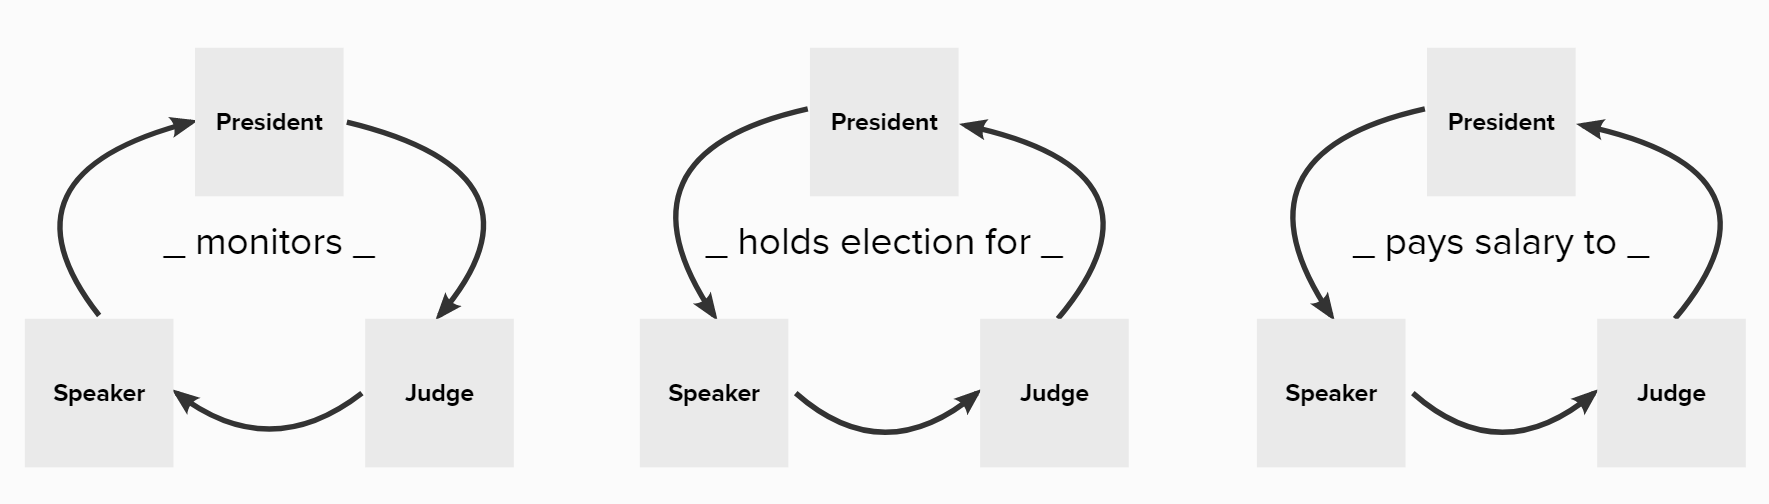
\includegraphics[scale=0.33]{05_iigo/images/role cycles.png}
\caption{Accountability cycle (left), the transfer-of-power cycle (middle) and salary cycle (right).}
\label{fig:cycles_in_IIGO}
\end{figure}


\subsection{Transfer-of-power}
\label{subsec:transfer-of-power}
\begin{enumerate}
    \item The Speaker conducts a vote for the election of the new Judge.
    \item The Judge conducts a vote for the election of the new President.
    \item The President conducts a vote for the election of the new Speaker.
\end{enumerate}
Refer to the Figure~ \ref{fig:cycles_in_IIGO} for further clarification about the transfer-of-power cycle.

\begin{rule_IIGO}
   The role $X$ has the \emph{obligation} to conduct a vote for the election of $Y$ at the end of the term (see Definition~\ref{def:term}) if and only if the role $X$ is accountable to the role $Y$. 
\end{rule_IIGO}.

\section{Budget and Salary}
\subsection{Budget}
%Actions associated with the IIGO have an associated cost that is defined as a configuration parameter. The institutional-power-enabled actions of  identified to require a "computational" component are:

Institutional-enabled-power actions in the IIGO have an associated cost with them. Some examples for such actions include:


%that is defined as a configuration parameter. The institutional-power-enabled actions of  identified to require a "computational" component are:


%We have defined the resource to be an endogenous one, hence any computation surrounding the distribution of the resource must use up some of that resource. 
\begin{itemize}
\item Calling any vote and computing the winner.
\item Declaring (e.g. \textit{announcing} the result of a vote).
\item Setting the amount of \emph{taxation} for each island.
\item Deciding the allocation distribution for each island.
\item Inspecting an island's action history.
\item Monitoring a role.
\end{itemize}

Since IIGO has been designed to act in the common good, IIGO-related costs will be directly withdrawn from the common pool. Since the common pool is considered a communal property of the archipelago, there are rules in place to limit how much each role is allowed to spend in order to perform its own institutional-power-enabled actions. This is the reason why defining the \emph{budget} and keeping it separate for each of the three IIGO roles.


As a role performs institutional-enabled-power actions, the corresponding cost associated with this action is subtracted from the role's budget. A budget of zero means that the role does not have the \emph{power} to perform any of its institutional-power-enabled actions. The removal of the budget rule from the rules in play means the role is allowed to perform as many such actions as it prefers to (as long as those actions are not governed by other rules). 



%As a role performs an endogenous-cost action, the corresponding cost associated with this action is subtracted from the role's budget. Thus, if as a result of an endogenous-cost action a role will be left with negative budget, it will have gone over the budget limit and will have broken the budget rule. A budget of zero means that the role is not allowed to perform any of its institutional-power-enabled actions associated an endogenous-cost. The removal of the budget rule from the rules in play means the role is allowed to perform as many such actions as it pleases (as long as those actions are not governed by other rules). 

The budget rule is also persistent across turns. This means that, assuming nothing else affects the budget, if a role has $100$ resources in its budget at each turn and spends only $10$ resources, this means that this very same role has $90$ resources in its budget at the next turn. On the other hand, islands can choose to increase the budget periodically every turn. This is governed by another budget extension rule.




%one turn and it spends 10, it has 90 resources in it's budget the next turn. 

Finally, it must be noted that the budget is inherently linked with the fact that whether obligations of a specific role can be undergone.
For example, during \emph{monitoring}, it should not be seen as a rule violation if a role has not acted on an obligation if it would go over the budget as a result. 

%This can also be seen as an added clause "... and the action is only permitted if they have the budget" to most rules which govern actions with an endogenous-cost.
%\begin{rule_IIGO}
    %The budget is increased by an amount $N$ every turn.
%\end{rule_IIGO}

%This rule means that, assuming nothing else affects the budget, if a budget is set to increase by 10 resources every turn and the budget is a 100 resources in turn one, the budget is 110 resources in turn 2. Setting this rule to 0 is equal to removing this rule and it means that the budget is never increased. 


\subsection{Salary}
\label{subsec:salary}
A salary is paid to each role in power as an incentive to act in a publicly approved way. %Hence, each role has the \emph{power} to pay a salary to another role following the salary cycle in Figure~\ref{fig:cycles_in_IIGO}.
\begin{rule_IIGO} \label{rule:salary}
   %Each role has the \emph{obligation} to pay the salary of amount $S$ to another if and only if the amount paid $S'$ is equal to $S$.
   Each role has the \emph{obligation} to pay the salary of amount $S$ to one another following the salary cycle in Figure~\ref{fig:cycles_in_IIGO}.
\end{rule_IIGO}

In Rule~\ref{rule:salary}, setting $S=0$ (through changing the active rules in place) means that roles do not have the permission to pay any salary. Removing the Rule~\ref{rule:salary} means that the roles may freely choose the amount $S$ for the salary payments.

\section{IIGO Session order}

\begin{enumerate}
    \item The Judge has the \emph{power} to check the history of actions to confirm whether the previously punished island(s) has/have obeyed the previous round's sanctions, meaning whether they contributed to the common pool accordingly in case of economic sanctions.
    %\begin{itemize}
      %  \item \emph{Suggested Rule:} In case of disobeying sanctions, the Judge is \emph{obliged} and \emph{permitted} to increase the severity of sanctions with respect to specific islands.
   % \end{itemize}
    \item The Judge has the \emph{power} to carry out \emph{inspections} on the history of actions of any island $X$ to check whether:
        \begin{enumerate}
        \item the reported resources of $X$ in the previous round match the real value of resources $X$ had in its private pool for the previous turn.
        \item the island $X$ has retrieved the right amount of the resources from the common pool, based on the \emph{allocation request} evaluated by the previous President.
            \begin{itemize}
            \item An example: In the previous round, the President has decided that the island $X$ can take $Y$ amount of resources from the common pool. If the Judge finds out that the island $X$ has taken an amount of $Y'$ such that $Y' > Y$, the Judge has the \emph{power} to invoke sanctions on the island $X$.
            
            %the Judge is \emph{obliged} and \emph{permitted} to sanction island $X$.
            \end{itemize}
        \end{enumerate}
    \item The Judge has the \emph{power} to invoke sanctions based on the outcome of the inspections.
    \item The President has the \emph{power} to decide to carry out a \emph{monitoring} on:
        \begin{enumerate}
        \item the sanctions imposed by the Judge.
        \end{enumerate}
    \item The islands may report the resources in their private pools to the President.
    \item The President has the \emph{power} to let each island know about the amount of \emph{taxation} they have to pay.
    \item The island has the \emph{power} to make an \emph{allocation request} to the President.
    \item The President has the \emph{power} decide on an allocation of resources and let each island know about the amount of resource allocation they are permitted to take from the common pool.
    \item The island has the \emph{power} to pick and to propose a rule to be voted on to the President.
    \item The President has the \emph{power} to choose a rule to be voted on from the received rule proposals.
    \item The Speaker has the \emph{power} to decide to carry out a \emph{monitoring} on: 
        \begin{enumerate}
        \item the resource allocation decided by the President.
        \item the rule proposed by the President.
        \end{enumerate}
    \item The Speaker has the \emph{power} to call a vote.
        \begin{enumerate}
        \item The islands vote in support of, or against, the rule (aye or nay) anonymously.
        \end{enumerate}
    \item The Speaker has the \emph{power} to announce a result of a vote to the islands and carries out the law change, if required (e.g. deleting/rejecting a rule if there is a majority nay vote).
    \item The Judge has the \emph{power} to decide to carry out \emph{monitoring} on:
        \begin{enumerate}
        \item the vote called by the Speaker.
        \item the Speaker announcing the result.
    \end{enumerate}
    \item The roles pay salary for one another following the accountability cycle in Figure~ \ref{fig:cycles_in_IIGO}.

\end{enumerate}



\section{Future Work}

\begin{itemize}
    \item \textbf{Diplomatic sanctions}: Although having the potential of being a good alternative for severer sanctions discussed in  Section~\ref{sec:sanctions}, diplomatic sanctions are \emph{not} implemented within the scope of the coursework. \\
    Suggested diplomatic sanctions include:
        \begin{itemize}
            \item Revoking an island's eligibility to vote and to be elected for a position.
            \item Revoking an island's eligibility to propose a rule/motion.
        \end{itemize}
    \item \textbf{Immutable rules}: Within the scope of the coursework, a subset of rules could have been categorised as immutable. This means that to change such immutable rules, the islands first need to vote to change their status to be \emph{mutable}, and consequently, hold another vote to change these mutable rules.
    %\item \textbf{Adding rules to the proposal list: } 
\end{itemize}

    \chapter{Inter-Island Governmental Organisation (IIGO)}


The role of IIGO is to maintain, update, and revise the rules concerning provision to managing the long-term collective risk dilemma (ltCRD). 

\begin{itemize}
    \item There will be 3 distinct branches in the IIGO: the \textbf{legislative branch}, \textbf{executive branch} and \textbf{judicial branch}\footnote{This is, as no surprise, inspired by the separation of powers in Western democracies.}.
    \item Each role is put in power according to the  transfer-of-power rules (see Section~\ref{subsec:transfer-of-power} for more detail).
    \item The head of the legislative branch is the Speaker, the head of the executive branch is the President, and the head of judicial branch is the Judge.
    \begin{itemize}
        \item  The Speaker, President and Judge are selected, through a democratic election, from the islands in the archipelago\footnote{This naming is inspired by the roles in the US Government.}.
        \item The resources gathered by the archipelago are endogenous, hence acting on the institutional powers granted to the Speaker, President or Judge costs resources. 
        \item For their duty, the President, the Speaker and the Judge receive a salary for each of their turns in office (see Section~\ref{subsec:salary} for more detail).
        \item The limit of the powers of the President, Speaker and Judge are defined in this chapter (e.g. the Speaker can only call one vote per turn).
 
    \end{itemize}
\end{itemize}

\subsection{IIGO Specific Definitions}
\begin{definition} \label{def:ballot}
    A \textbf{ballot} is related to each island's \textbf{power} to support or disagree with the rule specified in the vote called by the President and to vote in favour or against an island for a specific role (i.e. the President, Speaker, Judge) at each round of the game.
\end{definition}


%\begin{definition} \label{def:vote}
    %A \textbf{vote} is related to a role's (i.e. the President, Speaker, Judge) \textbf{power} to call a vote for a specific rule or an election.
%\end{definition}


\begin{definition} \label{def:tax}
    The \textbf{taxation} is related to the President's \textbf{power} to request a specific \underline{\textbf{minimum}} amount of contribution from each island to the common pool at each round of the game. 
\end{definition}

\begin{definition} \label{def:alloc_req}
    An \textbf{allocation request} is related to each island's \textbf{power} to request a specific amount of resource allocation from the President at each round of the game.
\end{definition}


\begin{definition} \label{def:rule_prop_list}
A \textbf{rule proposal list} is related to each island's \textbf{power} to propose a specific rule to be passed to the President at each round of the game.
\end{definition}

\begin{definition} \label{def:invst}
    An \textbf{investigation} is related to the Judge's \textbf{power} to acquire information to make a decision, followed by a calculation of the expected results and checking whether some specific rules have been obeyed, exclusively for the actions carried out by the \textbf{islands}. 
\end{definition}


An example of an \emph{investigation}: The President has permitted the island $X$ to take the amount of $Y$ resources from the common pool. Upon \emph{investigation} carried out by the Judge, it is revealed that the amount of resources taken out from the common pool by the island $X$ is, in fact, $Y'$ such that $Y' \neq Y$.


\begin{definition}
\textbf{Monitoring} is a government official's \textbf{power} to perform event recognition and to check whether some specific rules have been obeyed.
\end{definition}

An example of \emph{monitoring}: The Speaker has performed only the following action: \emph{counted the votes and calculated the result} for a rule. Upon \emph{monitoring} carried out by the President, it is noticed that the Speaker has not made any \emph{announcement}. Hence, the Speaker has not followed their obligation to \emph{announce} the result of any vote held.

See Section~\ref{sec:accountability} for more information about which roles can monitor which ones.


\begin{definition}
\textbf{Investigative-monitoring} is a government official's \textbf{power} to acquire the information used in acting on a governmental power followed by calculation of the expected results and checking whether some specific rules have been obeyed, exclusively for the actions carried out by a government official they are responsible for.
\end{definition}

An example of \emph{investigative-monitoring}: The Speaker has performed the following actions: \emph{counted the votes and calculated the result $R$} for a vote $V$ and \emph{announced} the result $R'$ for the vote $V$. Upon \emph{investigative-monitoring} carried out by the President, it is noticed that $R' \neq R$. Hence, the Speaker has modified the announced result.


\begin{definition}
The \textbf{sanction} is related to the Judge's \emph{power} to punish non-compliant islands when their disobedience is confirmed through investigations at a specific turn.
\end{definition}


\begin{definition}
The (judicial) \textbf{pardon} is related to the Judge's \emph{power} to forgive a non-compliant island at a specific turn.
\end{definition}

\begin{definition}
The \textbf{budget} is the maximum amount of resources a role is permitted to spend from the common pool as it performs its own institutional-power-enabled actions at a specific turn.
\end{definition}


\begin{definition}
The \textbf{salary} is the amount of resources a role is to be given from the common pool as a reward for performing its institutional-power-enabled actions at a specific turn.
\end{definition}

\begin{definition} \label{def:term}
A \textbf{term} is the number of turns an island is \emph{permitted} to hold a role, and after which the responsible role (indicated in the transfer-of-power cycle in Figure~\ref{fig:cycles_in_IIGO}) is \emph{obliged} to initiate transfer-of-power.
\end{definition}

\subsection{\emph{Power}, \emph{Permission} and \emph{Obligation} Distinction}
In the rest of the specifications, we will be specifically using the following three terms to define the actions and responsibilities carried out by the Speaker, President, Judge (see Figure~ \ref{fig:per_obl_sets}):
\begin{itemize}
    \item Power
    \item Permission
    \item Obligation
\end{itemize}



\begin{figure}[H] 
\centering
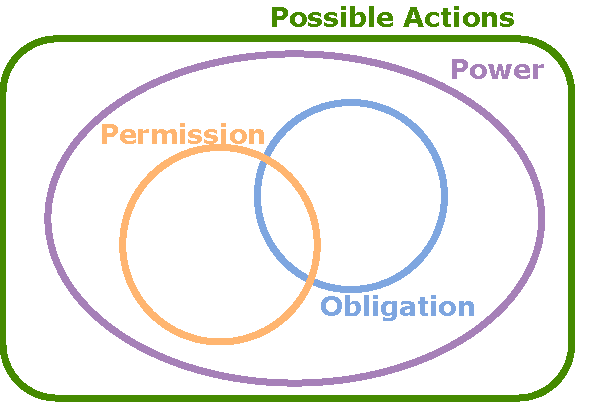
\includegraphics[width=0.6\textwidth]{05_iigo/images/SOMAS_per_obl.pdf}
\caption{Relationship between \emph{power}, \emph{permission} and \emph{obligation}.}
\label{fig:per_obl_sets}
\end{figure} 


For example, the Judge has the \emph{power} to carry out investigations at an IIGO session. There are no rules specifying which specific islands the Judge should investigate. Therefore, the Judge has the \emph{permission} to investigate any `alive' islands during a session. However, the Judge is \emph{obliged} to make at least some number of investigations each turn.



\section{Executive Branch}
\label{sec:executive}
The executive branch is responsible for \textbf{carrying out the law}.
\begin{itemize}
       
    \item The President has the \emph{power} to: 
    \begin{itemize}
        
        \item Select a rule for voting $R^{*}$ to be passed to the Speaker.
        \begin{rule_IIGO}
            The President has the \emph{obligation} to \emph{select} a rule $R^{*}$ if the \emph{rule proposal list} has at least one proposed rule in it.
        \end{rule_IIGO}
        \begin{rule_IIGO}
            The President has the \emph{permission} to \emph{select} a rule $R^{*}$ if and only if $R^{*} \in S$, where $S$ is the \emph{rule proposal list}.
        \end{rule_IIGO}
        
        \item Decide the amount of individual \emph{taxation} (i.e. a specific \emph{minimum} amount of contribution to the common pool for each island) for the current turn.
        
        \begin{itemize}
            \item The President is given the self-reported resource amounts held by each island to assist in this decision.
            %\item Suggested Rule: For any island that has chosen to not report it's resources, the President has the \emph{obligation} to set them an individual tax amount T.
        \end{itemize}
        
        \item Decide the allocation of resources distributed from the common pool to the islands (i.e. a specific \emph{maximum} amount an island is permitted to take from the common pool).
        
        \begin{itemize}
            \item The President is given the \emph{allocation requests} made by each island.
            %\item \emph{}{Suggested Rule:} The President has an obligation to prioritise islands in critical condition.
        \end{itemize}
    \end{itemize}
\end{itemize}



\section{Legislative Branch}
\label{sec:legislative}
The legislative branch is responsible for \textbf{making the law}.
\begin{itemize}

    \item The Speaker has the \emph{power} to:
    \begin{itemize}
        
        \item Call a vote $V$ for a rule $R$.
        \begin{rule_IIGO}
            The Speaker has the \emph{obligation} to \emph{call} a vote $V$ if and only if the President has \emph{selected} a rule $R$ to be voted on.
        \end {rule_IIGO}
        \begin{rule_IIGO}
            The Speaker has the \emph{permission} to \emph{call} a vote $V$ for a rule $R$ if and only if the rule $R = R^{*}$, where $R^{*}$ is the rule \emph{selected} by the President.
        \end {rule_IIGO}
            
        \item Choose which islands are participating in the vote $V$.
       % \footnote{This is our sequential implementation alternative for the power to close the ballot box.}.
        \begin{rule_IIGO}
            The Speaker has the \emph{obligation} to ask for a vote from all alive islands.
        \end {rule_IIGO}
            
        \item Declare the result $C$ of a vote $V$. 
        \begin{rule_IIGO}
            The Speaker has the \emph{obligation} to \emph{declare the result} $C$ for a vote $V$ if and only if the vote V has been \emph{called}.
        \end {rule_IIGO}
        \begin{rule_IIGO}
            The Speaker has the \emph{permission} to \emph{declare the result} $C$ for a vote $V$ if $C = C^{*}$, where $C^{*}$ is the result produced by \emph{calling} the vote $V$.
        \end {rule_IIGO}
        \begin{itemize}
            \item This step is what enables a rule to be \emph{active}.
        \end{itemize}
    \end{itemize}
\end{itemize}




\section{Judicial Branch}
\label{sec:judicial}

The judicial branch is responsible for \textbf{evaluating the law}.
\begin{itemize}
    \item The Judge has the \emph{power} to:
    \begin{itemize}
        \item Perform a number of \emph{inspections}\footnote{An \emph{inspection} \textbf{costs} an expense of resources (See Definition~\ref{def:invst} for more detail).} $I$ and produce a compliance outcome $\mathbb{O}^{*}$\footnote{Note that the compliance outcome $\mathbb{O}^{*}$ considered is a boolean.}.
        %(true: the island has been compliant with the rules in play, false: the island has not been compliant with the rules in play)
        %\begin{itemize}
           % \item For example, to check if the event outcome is \emph{concurrent}\footnote{Again, what is defined as "concurrent"? A clear definition is needed.} with the rules.
        %\end{itemize}
        \begin{rule_IIGO}
            The Judge has the \emph{obligation} to make at least $N$ investigations at each turn.
        \end{rule_IIGO}
        \item Declare the outcome $\mathbb{O}$ of an inspection $I$ to all islands\footnote{This act of broadcasting is especially important for islands to form an opinion about the sanctioned islands accordingly.}.
        \begin{rule_IIGO}
            The Judge has the \emph{obligation} to declare the outcome $\mathbb{O}$ of an inspection $I$ if and only if the inspection $I$ has been performed.
        \end{rule_IIGO}
        \begin{rule_IIGO}
            The Judge has the \emph{permission} to declare the outcome $\mathbb{O}$ of an inspection $I$ if $\mathbb{O} = \mathbb{O}^{*}$, where $\mathbb{O}^{*}$ is the outcome of the inspection $I$.
        \end{rule_IIGO}
        %\item Initiate the removal of the \texttt{President}.
        %\begin{itemize}
            %\item A good Judge would be especially vigilant during \emph{power transfer} regarding the \emph{President} position (see Section~\ref{leg_const} for more detail).
        %\end{itemize}
        \item Invoke economic \textbf{sanctions} (see Section~\ref{sec:sanctions} for more detail).
        \begin{rule_IIGO}
            The Judge has the \emph{obligation} to invoke a sanction $S$ for an island $X$ if and only if an investigation $I$ has an outcome $\mathbb{O}^{*}$ indicating non-compliance, and $I$ is an investigation of an action taken by island $X$.
        \end{rule_IIGO}
        \item Invoke even more severe sanctions in the case of further disobedience to previous sanction(s).
        \begin{rule_IIGO}
            The Judge has the \emph{permission} to invoke a severer sanction $S'$ for an island $X$ if the island $X$ has not fulfilled the requirements of the previous sanction $S$.
        \end{rule_IIGO}
        \item Pardon the islands which are currently sanctioned.
        \begin{rule_IIGO}
            The Judge has the \emph{permission} to revoke any sanction $S$ of an island $X$ at a specific turn.
        \end{rule_IIGO}
    \end{itemize}
\end{itemize}
%(e.g. a new rule that falls under a "sanction" category \hl{[I'm not sure about this being a `new rule` [Ezgi]]}

\subsection{Sanctions}
\label{sec:sanctions}
All sanctions are of economic nature which include:
        \begin{itemize}
            %\item Revoking an island's access to the common pool.
            \item Enforcing an island to contribute a specific amount of resources to the common pool.
            \begin{itemize}
                \item This does not mean that the Judge has the \emph{power} to take resources from an island in order to put them to the common pool -- the island itself is expected to carry out this implication imposed by the sanction itself, otherwise further punishment can be induced by the Judge.
                \item Similarly, \emph{opinion formulation} will follow accordingly whether the island(s) is/are following the implications imposed by the sanction(s).
            \end{itemize}
        
    \end{itemize}
    Sanctions are the associated penalty that comes with an island breaking a specific rule. The Judge is in full control of the penalties associated with breaking any rules. Once the Judge has specified the score of the penalty associated with each time an island breaks a rule, the cumulative penalties accumulated by the island are then used to determine which \textbf{sanction tier} that each island falls into. The score threshold to determine the boundaries of the sanction tiers are set by the Judge. At each turn of the game, each island is told whether they are being sanctioned, and if so, which \textbf{sanction tier} that they are currently in. The \textbf{sanction tiers} of the non-compliant islands are also broadcasted to the other islands in the archipelago. To summarise, the sanctioning process follows these steps:
    
    
    
    %Sanctions are based on an island breaking a rule. Each rule must therefore have an associated penalty. By default, we set these penalties such that they add $1$ to the total sanction score for each island. However, we allow the judge to override this scoring, the judge is able to set their own scores for any particular rule as they desire. This custom scoring is then used when an island breaks a particular rule. By looking at events that occurred in the last turn, and using the customised scoring we provide the holder of the judge role with full control of the penalties for breaking any rules.
    
    





%we then use the cumulative penalties accumulated by each island to determine which Sanction Tier they fall into. The score threshold's required to fall into these sanction tiers is set by the judge and is checked for monotonicity. Each island is told whether they are being sanctioned, and is so what tier they are in. We also tell other islands about which sanction tiers other islands have fallen into. 

    \begin{enumerate}
        \item The Judge has the \emph{power} to set custom penalties associated with breaking any rules.
        \item The Judge is given a list of all events that occurred in the previous turn.
        \item The Judge has the \emph{power} to check whether any, or all of these previous events, involve the islands in the archipelago breaking any rules.
        \item Each of the transgressions is scored using the Judge's custom penalties if the Judge has set them. Otherwise, a score of $1$ is given each time a rule is broken.
        \item The Judge has the \emph{power} to revise the sanction thresholds.
        \item Using the latest sanction thresholds available, each island is assigned to a sanction tier based on the sanction score that it has received.
        \item These sanction tiers are broadcasted to all of the islands in the archipelago.
        \item The Judge then uses sanctions rules in place to calculate the specific amount of resources that each non-compliant island has in order to determine how much it should contribute to the common pool, based on the sanction tier that it is in.
    \end{enumerate}



\section{Constitutional Rights and Obligations in the Archipelago}
\label{sec:const_rights_obl_archi}
Each island has the \emph{power} to:
\begin{itemize}
\item make an \emph{allocation request} (see Definition~\ref{def:alloc_req}) to the President for a specific amount to be allocated to them.
\item report the number of resources it is in possession of to the President.
\begin{rule_IIGO}
    Each island has the \emph{obligation} to report the number of resources it is in possession of to the President.
\end{rule_IIGO}
\begin{rule_IIGO}
    Each island has the \emph{permission} to report the number of resources $R'$ if and only if $R' = R$, where R is the number of resources the island is in possession of.
\end{rule_IIGO}
\item take resources from the common pool.


\begin{rule_IIGO}
    Each island has the \emph{permission} to take at maximum $N$ resources, where $N$ is the specific allocation made by the President to that island\footnote{If no such allocation is made, the island is \emph{permitted} to take any amount of resources.}.
\end{rule_IIGO}
\item contribute resources to the common pool.
\begin{rule_IIGO}
    Each island has the \emph{obligation} to contribute to the common pool an amount greater or equal to that of the individual tax set by the President.
\end{rule_IIGO}
                %The President is in
                %(unless there is a rule in place that dictates how Speaker is to allocate resources).
\item add a rule to the \emph{rule proposal list} (see Definition~\ref{def:rule_prop_list}) at the start of each turn.
        %\begin{itemize}
            %\item The game specification includes how many rules an island can propose each turn.
        %\end{itemize}
        %\item vote  for rules in the Legislative Branch and vote for their favourite islands in elections
\item participate in the legislative branch of the government by casting ballots in votes called by the Speaker
\item vote for an island to be elected for a specific role (e.g. the President, Judge, Speaker) during the elections\footnote{This will be assumed to be true \underline{unless stated otherwise}. %Note that \textbf{diplomatic sanctions} can disable this power of a specific island (see Section~\ref{jud_const}).}.
        }.
\end{itemize}
\section{Accountability Cycle}
\label{sec:accountability}


To ensure that the government avoids corruption and abuse of power, each branch is accountable to another. The President is accountable to the Speaker, the Speaker is accountable to the Judge, and the Judge is accountable to the President (see Figure~ \ref{fig:cycles_in_IIGO}). This accountability cycle is enacted through \emph{monitoring} actions\footnote{Note that the terms \textbf{monitoring} and \textbf{investigation} have similar but quite different meanings in the IIGO context.}. 

The powers related to the accountability cycle and transfer-of-power for each role can be summarized as the following: 
\begin{itemize}
    \item The Speaker has the \emph{power} to: 
    \begin{itemize}
        \item monitor the President.
        \item announce the result of this monitoring.
        \item initiate the transfer-of-power for the Judge.
    \end{itemize}
    \item The President has the \emph{power} to: 
    \begin{itemize}
        \item monitor the Judge.
        \item announce the result of this monitoring.
        \item initiate the transfer-of-power for the Speaker.
    \end{itemize}
    \item The Judge has the \emph{power} to: 
    \begin{itemize}
        \item  monitor the Speaker.
        \item announce the result of this monitoring.
        \item initiate the transfer-of-power for the President.
    \end{itemize}
\end{itemize}

%Unlike investigations performed by the Judge, who performs investigations on island actions in the following turn, each role is given the opportunity to check up on the actions of the role it is responsible for immediately after they have been performed. In this sense, the President can monitor (includes investigative-monitoring) the powers (calling a vote and announcing the result) acted on by the Speaker immediately after the Speaker's announcement (or lack there of). The government officials hold a lot of power so this is to ensure that any wrong-doing is determined as quickly as possible. For this project we are only pursuing one degree of monitoring, that is, the powers relating to the accountability cycle will not be monitored themselves. We assume that agents will act in the interest of themselves and keeping all the islands alive is beneficial to everyone. Hence, while the agents might be inclined to break rules in order to benefit themselves, anyone else breaking the rules is seen as undesirable under the assumption that the system in place is there to benefit all. 


Through the proposed accountability cycle, each role is given the opportunity to check up on the actions of the role it is accountable for immediately after they have been performed. It is clear that the IIGO roles (i.e. the President, Speaker and Judge) hold a considerable amount of \emph{power} in their hands. The accountability cycle is designed to address the possible abuses of this power. With monitoring, any wrong-doing in the IGO is determined as quickly as possible and the role in question can be replaced. 

Within the scope of the coursework, we decided to pursue only \emph{one degree of monitoring}, meaning that the powers relating to the accountability cycle will not be monitored themselves. We assume that agents will act in the interest of all the islands in the archipelago. Hence, while the agents might be inclined to break the rules to benefit in some form, it is assumed that the others will negatively see any non-compliant islands based on the assumption that the proposed IIGO system is in place to maintain the welfare of all the islands.

Let role $X$ be accountable to the role $Y$, which is accountable to the role $Z$. Then:
\begin{rule_IIGO}
$Y$ has the \emph{obligation} to declare the outcome of the monitoring result $M$ associated with the action $A$ undertaken by $X$ if and only if $Y$ has monitored the action $A$ performed by $X$. 
\end{rule_IIGO}
\begin{rule_IIGO}
$Y$ has the \emph{permission} to declare the monitoring result $M$ associated with the action $A$ undertaken by $X$ if and only if $M = M^{*}$, where $M^{*}$ is the outcome of \emph{monitoring} action $A$ performed by $X$\footnote{These constitutional rules should be available to the agents to check their decision against. However, due to having only one degree of accountability cycle in place, these rules are not enforced through any sanctions (i.e. breaking these rules has no consequences as they only deem to be an \emph{agreement} among the roles).}.
\end{rule_IIGO}


\begin{figure}[!htb]
\centering
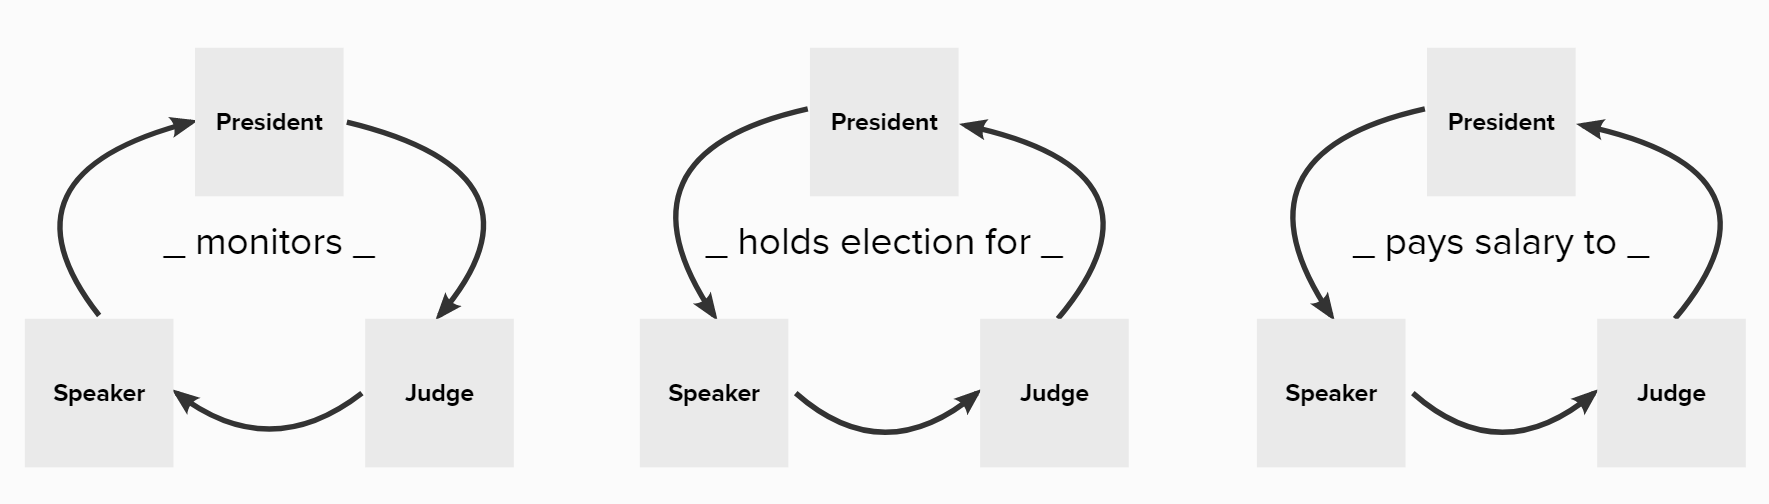
\includegraphics[scale=0.33]{05_iigo/images/role cycles.png}
\caption{Accountability cycle (left), the transfer-of-power cycle (middle) and salary cycle (right).}
\label{fig:cycles_in_IIGO}
\end{figure}


\subsection{Transfer-of-power}
\label{subsec:transfer-of-power}
\begin{enumerate}
    \item The Speaker conducts a vote for the election of the new Judge.
    \item The Judge conducts a vote for the election of the new President.
    \item The President conducts a vote for the election of the new Speaker.
\end{enumerate}
Refer to the Figure~ \ref{fig:cycles_in_IIGO} for further clarification about the transfer-of-power cycle.

\begin{rule_IIGO}
   The role $X$ has the \emph{obligation} to conduct a vote for the election of $Y$ at the end of the term (see Definition~\ref{def:term}) if and only if the role $X$ is accountable to the role $Y$. 
\end{rule_IIGO}.

\section{Budget and Salary}
\subsection{Budget}
%Actions associated with the IIGO have an associated cost that is defined as a configuration parameter. The institutional-power-enabled actions of  identified to require a "computational" component are:

Institutional-enabled-power actions in the IIGO have an associated cost with them. Some examples for such actions include:


%that is defined as a configuration parameter. The institutional-power-enabled actions of  identified to require a "computational" component are:


%We have defined the resource to be an endogenous one, hence any computation surrounding the distribution of the resource must use up some of that resource. 
\begin{itemize}
\item Calling any vote and computing the winner.
\item Declaring (e.g. \textit{announcing} the result of a vote).
\item Setting the amount of \emph{taxation} for each island.
\item Deciding the allocation distribution for each island.
\item Inspecting an island's action history.
\item Monitoring a role.
\end{itemize}

Since IIGO has been designed to act in the common good, IIGO-related costs will be directly withdrawn from the common pool. Since the common pool is considered a communal property of the archipelago, there are rules in place to limit how much each role is allowed to spend in order to perform its own institutional-power-enabled actions. This is the reason why defining the \emph{budget} and keeping it separate for each of the three IIGO roles.


As a role performs institutional-enabled-power actions, the corresponding cost associated with this action is subtracted from the role's budget. A budget of zero means that the role does not have the \emph{power} to perform any of its institutional-power-enabled actions. The removal of the budget rule from the rules in play means the role is allowed to perform as many such actions as it prefers to (as long as those actions are not governed by other rules). 



%As a role performs an endogenous-cost action, the corresponding cost associated with this action is subtracted from the role's budget. Thus, if as a result of an endogenous-cost action a role will be left with negative budget, it will have gone over the budget limit and will have broken the budget rule. A budget of zero means that the role is not allowed to perform any of its institutional-power-enabled actions associated an endogenous-cost. The removal of the budget rule from the rules in play means the role is allowed to perform as many such actions as it pleases (as long as those actions are not governed by other rules). 

The budget rule is also persistent across turns. This means that, assuming nothing else affects the budget, if a role has $100$ resources in its budget at each turn and spends only $10$ resources, this means that this very same role has $90$ resources in its budget at the next turn. On the other hand, islands can choose to increase the budget periodically every turn. This is governed by another budget extension rule.




%one turn and it spends 10, it has 90 resources in it's budget the next turn. 

Finally, it must be noted that the budget is inherently linked with the fact that whether obligations of a specific role can be undergone.
For example, during \emph{monitoring}, it should not be seen as a rule violation if a role has not acted on an obligation if it would go over the budget as a result. 

%This can also be seen as an added clause "... and the action is only permitted if they have the budget" to most rules which govern actions with an endogenous-cost.
%\begin{rule_IIGO}
    %The budget is increased by an amount $N$ every turn.
%\end{rule_IIGO}

%This rule means that, assuming nothing else affects the budget, if a budget is set to increase by 10 resources every turn and the budget is a 100 resources in turn one, the budget is 110 resources in turn 2. Setting this rule to 0 is equal to removing this rule and it means that the budget is never increased. 


\subsection{Salary}
\label{subsec:salary}
A salary is paid to each role in power as an incentive to act in a publicly approved way. %Hence, each role has the \emph{power} to pay a salary to another role following the salary cycle in Figure~\ref{fig:cycles_in_IIGO}.
\begin{rule_IIGO} \label{rule:salary}
   %Each role has the \emph{obligation} to pay the salary of amount $S$ to another if and only if the amount paid $S'$ is equal to $S$.
   Each role has the \emph{obligation} to pay the salary of amount $S$ to one another following the salary cycle in Figure~\ref{fig:cycles_in_IIGO}.
\end{rule_IIGO}

In Rule~\ref{rule:salary}, setting $S=0$ (through changing the active rules in place) means that roles do not have the permission to pay any salary. Removing the Rule~\ref{rule:salary} means that the roles may freely choose the amount $S$ for the salary payments.

\section{IIGO Session order}

\begin{enumerate}
    \item The Judge has the \emph{power} to check the history of actions to confirm whether the previously punished island(s) has/have obeyed the previous round's sanctions, meaning whether they contributed to the common pool accordingly in case of economic sanctions.
    %\begin{itemize}
      %  \item \emph{Suggested Rule:} In case of disobeying sanctions, the Judge is \emph{obliged} and \emph{permitted} to increase the severity of sanctions with respect to specific islands.
   % \end{itemize}
    \item The Judge has the \emph{power} to carry out \emph{inspections} on the history of actions of any island $X$ to check whether:
        \begin{enumerate}
        \item the reported resources of $X$ in the previous round match the real value of resources $X$ had in its private pool for the previous turn.
        \item the island $X$ has retrieved the right amount of the resources from the common pool, based on the \emph{allocation request} evaluated by the previous President.
            \begin{itemize}
            \item An example: In the previous round, the President has decided that the island $X$ can take $Y$ amount of resources from the common pool. If the Judge finds out that the island $X$ has taken an amount of $Y'$ such that $Y' > Y$, the Judge has the \emph{power} to invoke sanctions on the island $X$.
            
            %the Judge is \emph{obliged} and \emph{permitted} to sanction island $X$.
            \end{itemize}
        \end{enumerate}
    \item The Judge has the \emph{power} to invoke sanctions based on the outcome of the inspections.
    \item The President has the \emph{power} to decide to carry out a \emph{monitoring} on:
        \begin{enumerate}
        \item the sanctions imposed by the Judge.
        \end{enumerate}
    \item The islands may report the resources in their private pools to the President.
    \item The President has the \emph{power} to let each island know about the amount of \emph{taxation} they have to pay.
    \item The island has the \emph{power} to make an \emph{allocation request} to the President.
    \item The President has the \emph{power} decide on an allocation of resources and let each island know about the amount of resource allocation they are permitted to take from the common pool.
    \item The island has the \emph{power} to pick and to propose a rule to be voted on to the President.
    \item The President has the \emph{power} to choose a rule to be voted on from the received rule proposals.
    \item The Speaker has the \emph{power} to decide to carry out a \emph{monitoring} on: 
        \begin{enumerate}
        \item the resource allocation decided by the President.
        \item the rule proposed by the President.
        \end{enumerate}
    \item The Speaker has the \emph{power} to call a vote.
        \begin{enumerate}
        \item The islands vote in support of, or against, the rule (aye or nay) anonymously.
        \end{enumerate}
    \item The Speaker has the \emph{power} to announce a result of a vote to the islands and carries out the law change, if required (e.g. deleting/rejecting a rule if there is a majority nay vote).
    \item The Judge has the \emph{power} to decide to carry out \emph{monitoring} on:
        \begin{enumerate}
        \item the vote called by the Speaker.
        \item the Speaker announcing the result.
    \end{enumerate}
    \item The roles pay salary for one another following the accountability cycle in Figure~ \ref{fig:cycles_in_IIGO}.

\end{enumerate}



\section{Future Work}

\begin{itemize}
    \item \textbf{Diplomatic sanctions}: Although having the potential of being a good alternative for severer sanctions discussed in  Section~\ref{sec:sanctions}, diplomatic sanctions are \emph{not} implemented within the scope of the coursework. \\
    Suggested diplomatic sanctions include:
        \begin{itemize}
            \item Revoking an island's eligibility to vote and to be elected for a position.
            \item Revoking an island's eligibility to propose a rule/motion.
        \end{itemize}
    \item \textbf{Immutable rules}: Within the scope of the coursework, a subset of rules could have been categorised as immutable. This means that to change such immutable rules, the islands first need to vote to change their status to be \emph{mutable}, and consequently, hold another vote to change these mutable rules.
    %\item \textbf{Adding rules to the proposal list: } 
\end{itemize}

    \chapter{Inter-Island Governmental Organisation (IIGO)}


The role of IIGO is to maintain, update, and revise the rules concerning provision to managing the long-term collective risk dilemma (ltCRD). 

\begin{itemize}
    \item There will be 3 distinct branches in the IIGO: the \textbf{legislative branch}, \textbf{executive branch} and \textbf{judicial branch}\footnote{This is, as no surprise, inspired by the separation of powers in Western democracies.}.
    \item Each role is put in power according to the  transfer-of-power rules (see Section~\ref{subsec:transfer-of-power} for more detail).
    \item The head of the legislative branch is the Speaker, the head of the executive branch is the President, and the head of judicial branch is the Judge.
    \begin{itemize}
        \item  The Speaker, President and Judge are selected, through a democratic election, from the islands in the archipelago\footnote{This naming is inspired by the roles in the US Government.}.
        \item The resources gathered by the archipelago are endogenous, hence acting on the institutional powers granted to the Speaker, President or Judge costs resources. 
        \item For their duty, the President, the Speaker and the Judge receive a salary for each of their turns in office (see Section~\ref{subsec:salary} for more detail).
        \item The limit of the powers of the President, Speaker and Judge are defined in this chapter (e.g. the Speaker can only call one vote per turn).
 
    \end{itemize}
\end{itemize}

\subsection{IIGO Specific Definitions}
\begin{definition} \label{def:ballot}
    A \textbf{ballot} is related to each island's \textbf{power} to support or disagree with the rule specified in the vote called by the President and to vote in favour or against an island for a specific role (i.e. the President, Speaker, Judge) at each round of the game.
\end{definition}


%\begin{definition} \label{def:vote}
    %A \textbf{vote} is related to a role's (i.e. the President, Speaker, Judge) \textbf{power} to call a vote for a specific rule or an election.
%\end{definition}


\begin{definition} \label{def:tax}
    The \textbf{taxation} is related to the President's \textbf{power} to request a specific \underline{\textbf{minimum}} amount of contribution from each island to the common pool at each round of the game. 
\end{definition}

\begin{definition} \label{def:alloc_req}
    An \textbf{allocation request} is related to each island's \textbf{power} to request a specific amount of resource allocation from the President at each round of the game.
\end{definition}


\begin{definition} \label{def:rule_prop_list}
A \textbf{rule proposal list} is related to each island's \textbf{power} to propose a specific rule to be passed to the President at each round of the game.
\end{definition}

\begin{definition} \label{def:invst}
    An \textbf{investigation} is related to the Judge's \textbf{power} to acquire information to make a decision, followed by a calculation of the expected results and checking whether some specific rules have been obeyed, exclusively for the actions carried out by the \textbf{islands}. 
\end{definition}


An example of an \emph{investigation}: The President has permitted the island $X$ to take the amount of $Y$ resources from the common pool. Upon \emph{investigation} carried out by the Judge, it is revealed that the amount of resources taken out from the common pool by the island $X$ is, in fact, $Y'$ such that $Y' \neq Y$.


\begin{definition}
\textbf{Monitoring} is a government official's \textbf{power} to perform event recognition and to check whether some specific rules have been obeyed.
\end{definition}

An example of \emph{monitoring}: The Speaker has performed only the following action: \emph{counted the votes and calculated the result} for a rule. Upon \emph{monitoring} carried out by the President, it is noticed that the Speaker has not made any \emph{announcement}. Hence, the Speaker has not followed their obligation to \emph{announce} the result of any vote held.

See Section~\ref{sec:accountability} for more information about which roles can monitor which ones.


\begin{definition}
\textbf{Investigative-monitoring} is a government official's \textbf{power} to acquire the information used in acting on a governmental power followed by calculation of the expected results and checking whether some specific rules have been obeyed, exclusively for the actions carried out by a government official they are responsible for.
\end{definition}

An example of \emph{investigative-monitoring}: The Speaker has performed the following actions: \emph{counted the votes and calculated the result $R$} for a vote $V$ and \emph{announced} the result $R'$ for the vote $V$. Upon \emph{investigative-monitoring} carried out by the President, it is noticed that $R' \neq R$. Hence, the Speaker has modified the announced result.


\begin{definition}
The \textbf{sanction} is related to the Judge's \emph{power} to punish non-compliant islands when their disobedience is confirmed through investigations at a specific turn.
\end{definition}


\begin{definition}
The (judicial) \textbf{pardon} is related to the Judge's \emph{power} to forgive a non-compliant island at a specific turn.
\end{definition}

\begin{definition}
The \textbf{budget} is the maximum amount of resources a role is permitted to spend from the common pool as it performs its own institutional-power-enabled actions at a specific turn.
\end{definition}


\begin{definition}
The \textbf{salary} is the amount of resources a role is to be given from the common pool as a reward for performing its institutional-power-enabled actions at a specific turn.
\end{definition}

\begin{definition} \label{def:term}
A \textbf{term} is the number of turns an island is \emph{permitted} to hold a role, and after which the responsible role (indicated in the transfer-of-power cycle in Figure~\ref{fig:cycles_in_IIGO}) is \emph{obliged} to initiate transfer-of-power.
\end{definition}

\subsection{\emph{Power}, \emph{Permission} and \emph{Obligation} Distinction}
In the rest of the specifications, we will be specifically using the following three terms to define the actions and responsibilities carried out by the Speaker, President, Judge (see Figure~ \ref{fig:per_obl_sets}):
\begin{itemize}
    \item Power
    \item Permission
    \item Obligation
\end{itemize}



\begin{figure}[H] 
\centering
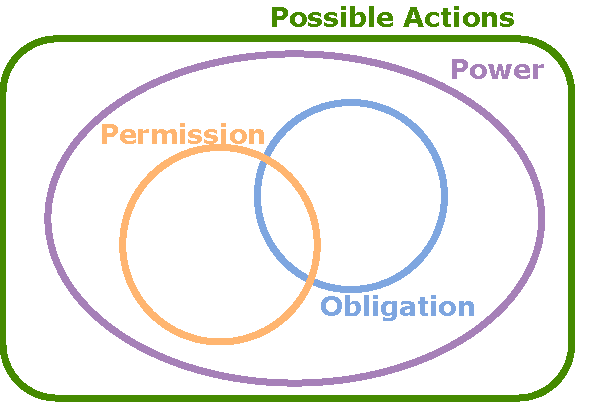
\includegraphics[width=0.6\textwidth]{05_iigo/images/SOMAS_per_obl.pdf}
\caption{Relationship between \emph{power}, \emph{permission} and \emph{obligation}.}
\label{fig:per_obl_sets}
\end{figure} 


For example, the Judge has the \emph{power} to carry out investigations at an IIGO session. There are no rules specifying which specific islands the Judge should investigate. Therefore, the Judge has the \emph{permission} to investigate any `alive' islands during a session. However, the Judge is \emph{obliged} to make at least some number of investigations each turn.



\section{Executive Branch}
\label{sec:executive}
The executive branch is responsible for \textbf{carrying out the law}.
\begin{itemize}
       
    \item The President has the \emph{power} to: 
    \begin{itemize}
        
        \item Select a rule for voting $R^{*}$ to be passed to the Speaker.
        \begin{rule_IIGO}
            The President has the \emph{obligation} to \emph{select} a rule $R^{*}$ if the \emph{rule proposal list} has at least one proposed rule in it.
        \end{rule_IIGO}
        \begin{rule_IIGO}
            The President has the \emph{permission} to \emph{select} a rule $R^{*}$ if and only if $R^{*} \in S$, where $S$ is the \emph{rule proposal list}.
        \end{rule_IIGO}
        
        \item Decide the amount of individual \emph{taxation} (i.e. a specific \emph{minimum} amount of contribution to the common pool for each island) for the current turn.
        
        \begin{itemize}
            \item The President is given the self-reported resource amounts held by each island to assist in this decision.
            %\item Suggested Rule: For any island that has chosen to not report it's resources, the President has the \emph{obligation} to set them an individual tax amount T.
        \end{itemize}
        
        \item Decide the allocation of resources distributed from the common pool to the islands (i.e. a specific \emph{maximum} amount an island is permitted to take from the common pool).
        
        \begin{itemize}
            \item The President is given the \emph{allocation requests} made by each island.
            %\item \emph{}{Suggested Rule:} The President has an obligation to prioritise islands in critical condition.
        \end{itemize}
    \end{itemize}
\end{itemize}



\section{Legislative Branch}
\label{sec:legislative}
The legislative branch is responsible for \textbf{making the law}.
\begin{itemize}

    \item The Speaker has the \emph{power} to:
    \begin{itemize}
        
        \item Call a vote $V$ for a rule $R$.
        \begin{rule_IIGO}
            The Speaker has the \emph{obligation} to \emph{call} a vote $V$ if and only if the President has \emph{selected} a rule $R$ to be voted on.
        \end {rule_IIGO}
        \begin{rule_IIGO}
            The Speaker has the \emph{permission} to \emph{call} a vote $V$ for a rule $R$ if and only if the rule $R = R^{*}$, where $R^{*}$ is the rule \emph{selected} by the President.
        \end {rule_IIGO}
            
        \item Choose which islands are participating in the vote $V$.
       % \footnote{This is our sequential implementation alternative for the power to close the ballot box.}.
        \begin{rule_IIGO}
            The Speaker has the \emph{obligation} to ask for a vote from all alive islands.
        \end {rule_IIGO}
            
        \item Declare the result $C$ of a vote $V$. 
        \begin{rule_IIGO}
            The Speaker has the \emph{obligation} to \emph{declare the result} $C$ for a vote $V$ if and only if the vote V has been \emph{called}.
        \end {rule_IIGO}
        \begin{rule_IIGO}
            The Speaker has the \emph{permission} to \emph{declare the result} $C$ for a vote $V$ if $C = C^{*}$, where $C^{*}$ is the result produced by \emph{calling} the vote $V$.
        \end {rule_IIGO}
        \begin{itemize}
            \item This step is what enables a rule to be \emph{active}.
        \end{itemize}
    \end{itemize}
\end{itemize}




\section{Judicial Branch}
\label{sec:judicial}

The judicial branch is responsible for \textbf{evaluating the law}.
\begin{itemize}
    \item The Judge has the \emph{power} to:
    \begin{itemize}
        \item Perform a number of \emph{inspections}\footnote{An \emph{inspection} \textbf{costs} an expense of resources (See Definition~\ref{def:invst} for more detail).} $I$ and produce a compliance outcome $\mathbb{O}^{*}$\footnote{Note that the compliance outcome $\mathbb{O}^{*}$ considered is a boolean.}.
        %(true: the island has been compliant with the rules in play, false: the island has not been compliant with the rules in play)
        %\begin{itemize}
           % \item For example, to check if the event outcome is \emph{concurrent}\footnote{Again, what is defined as "concurrent"? A clear definition is needed.} with the rules.
        %\end{itemize}
        \begin{rule_IIGO}
            The Judge has the \emph{obligation} to make at least $N$ investigations at each turn.
        \end{rule_IIGO}
        \item Declare the outcome $\mathbb{O}$ of an inspection $I$ to all islands\footnote{This act of broadcasting is especially important for islands to form an opinion about the sanctioned islands accordingly.}.
        \begin{rule_IIGO}
            The Judge has the \emph{obligation} to declare the outcome $\mathbb{O}$ of an inspection $I$ if and only if the inspection $I$ has been performed.
        \end{rule_IIGO}
        \begin{rule_IIGO}
            The Judge has the \emph{permission} to declare the outcome $\mathbb{O}$ of an inspection $I$ if $\mathbb{O} = \mathbb{O}^{*}$, where $\mathbb{O}^{*}$ is the outcome of the inspection $I$.
        \end{rule_IIGO}
        %\item Initiate the removal of the \texttt{President}.
        %\begin{itemize}
            %\item A good Judge would be especially vigilant during \emph{power transfer} regarding the \emph{President} position (see Section~\ref{leg_const} for more detail).
        %\end{itemize}
        \item Invoke economic \textbf{sanctions} (see Section~\ref{sec:sanctions} for more detail).
        \begin{rule_IIGO}
            The Judge has the \emph{obligation} to invoke a sanction $S$ for an island $X$ if and only if an investigation $I$ has an outcome $\mathbb{O}^{*}$ indicating non-compliance, and $I$ is an investigation of an action taken by island $X$.
        \end{rule_IIGO}
        \item Invoke even more severe sanctions in the case of further disobedience to previous sanction(s).
        \begin{rule_IIGO}
            The Judge has the \emph{permission} to invoke a severer sanction $S'$ for an island $X$ if the island $X$ has not fulfilled the requirements of the previous sanction $S$.
        \end{rule_IIGO}
        \item Pardon the islands which are currently sanctioned.
        \begin{rule_IIGO}
            The Judge has the \emph{permission} to revoke any sanction $S$ of an island $X$ at a specific turn.
        \end{rule_IIGO}
    \end{itemize}
\end{itemize}
%(e.g. a new rule that falls under a "sanction" category \hl{[I'm not sure about this being a `new rule` [Ezgi]]}

\subsection{Sanctions}
\label{sec:sanctions}
All sanctions are of economic nature which include:
        \begin{itemize}
            %\item Revoking an island's access to the common pool.
            \item Enforcing an island to contribute a specific amount of resources to the common pool.
            \begin{itemize}
                \item This does not mean that the Judge has the \emph{power} to take resources from an island in order to put them to the common pool -- the island itself is expected to carry out this implication imposed by the sanction itself, otherwise further punishment can be induced by the Judge.
                \item Similarly, \emph{opinion formulation} will follow accordingly whether the island(s) is/are following the implications imposed by the sanction(s).
            \end{itemize}
        
    \end{itemize}
    Sanctions are the associated penalty that comes with an island breaking a specific rule. The Judge is in full control of the penalties associated with breaking any rules. Once the Judge has specified the score of the penalty associated with each time an island breaks a rule, the cumulative penalties accumulated by the island are then used to determine which \textbf{sanction tier} that each island falls into. The score threshold to determine the boundaries of the sanction tiers are set by the Judge. At each turn of the game, each island is told whether they are being sanctioned, and if so, which \textbf{sanction tier} that they are currently in. The \textbf{sanction tiers} of the non-compliant islands are also broadcasted to the other islands in the archipelago. To summarise, the sanctioning process follows these steps:
    
    
    
    %Sanctions are based on an island breaking a rule. Each rule must therefore have an associated penalty. By default, we set these penalties such that they add $1$ to the total sanction score for each island. However, we allow the judge to override this scoring, the judge is able to set their own scores for any particular rule as they desire. This custom scoring is then used when an island breaks a particular rule. By looking at events that occurred in the last turn, and using the customised scoring we provide the holder of the judge role with full control of the penalties for breaking any rules.
    
    





%we then use the cumulative penalties accumulated by each island to determine which Sanction Tier they fall into. The score threshold's required to fall into these sanction tiers is set by the judge and is checked for monotonicity. Each island is told whether they are being sanctioned, and is so what tier they are in. We also tell other islands about which sanction tiers other islands have fallen into. 

    \begin{enumerate}
        \item The Judge has the \emph{power} to set custom penalties associated with breaking any rules.
        \item The Judge is given a list of all events that occurred in the previous turn.
        \item The Judge has the \emph{power} to check whether any, or all of these previous events, involve the islands in the archipelago breaking any rules.
        \item Each of the transgressions is scored using the Judge's custom penalties if the Judge has set them. Otherwise, a score of $1$ is given each time a rule is broken.
        \item The Judge has the \emph{power} to revise the sanction thresholds.
        \item Using the latest sanction thresholds available, each island is assigned to a sanction tier based on the sanction score that it has received.
        \item These sanction tiers are broadcasted to all of the islands in the archipelago.
        \item The Judge then uses sanctions rules in place to calculate the specific amount of resources that each non-compliant island has in order to determine how much it should contribute to the common pool, based on the sanction tier that it is in.
    \end{enumerate}



\section{Constitutional Rights and Obligations in the Archipelago}
\label{sec:const_rights_obl_archi}
Each island has the \emph{power} to:
\begin{itemize}
\item make an \emph{allocation request} (see Definition~\ref{def:alloc_req}) to the President for a specific amount to be allocated to them.
\item report the number of resources it is in possession of to the President.
\begin{rule_IIGO}
    Each island has the \emph{obligation} to report the number of resources it is in possession of to the President.
\end{rule_IIGO}
\begin{rule_IIGO}
    Each island has the \emph{permission} to report the number of resources $R'$ if and only if $R' = R$, where R is the number of resources the island is in possession of.
\end{rule_IIGO}
\item take resources from the common pool.


\begin{rule_IIGO}
    Each island has the \emph{permission} to take at maximum $N$ resources, where $N$ is the specific allocation made by the President to that island\footnote{If no such allocation is made, the island is \emph{permitted} to take any amount of resources.}.
\end{rule_IIGO}
\item contribute resources to the common pool.
\begin{rule_IIGO}
    Each island has the \emph{obligation} to contribute to the common pool an amount greater or equal to that of the individual tax set by the President.
\end{rule_IIGO}
                %The President is in
                %(unless there is a rule in place that dictates how Speaker is to allocate resources).
\item add a rule to the \emph{rule proposal list} (see Definition~\ref{def:rule_prop_list}) at the start of each turn.
        %\begin{itemize}
            %\item The game specification includes how many rules an island can propose each turn.
        %\end{itemize}
        %\item vote  for rules in the Legislative Branch and vote for their favourite islands in elections
\item participate in the legislative branch of the government by casting ballots in votes called by the Speaker
\item vote for an island to be elected for a specific role (e.g. the President, Judge, Speaker) during the elections\footnote{This will be assumed to be true \underline{unless stated otherwise}. %Note that \textbf{diplomatic sanctions} can disable this power of a specific island (see Section~\ref{jud_const}).}.
        }.
\end{itemize}
\section{Accountability Cycle}
\label{sec:accountability}


To ensure that the government avoids corruption and abuse of power, each branch is accountable to another. The President is accountable to the Speaker, the Speaker is accountable to the Judge, and the Judge is accountable to the President (see Figure~ \ref{fig:cycles_in_IIGO}). This accountability cycle is enacted through \emph{monitoring} actions\footnote{Note that the terms \textbf{monitoring} and \textbf{investigation} have similar but quite different meanings in the IIGO context.}. 

The powers related to the accountability cycle and transfer-of-power for each role can be summarized as the following: 
\begin{itemize}
    \item The Speaker has the \emph{power} to: 
    \begin{itemize}
        \item monitor the President.
        \item announce the result of this monitoring.
        \item initiate the transfer-of-power for the Judge.
    \end{itemize}
    \item The President has the \emph{power} to: 
    \begin{itemize}
        \item monitor the Judge.
        \item announce the result of this monitoring.
        \item initiate the transfer-of-power for the Speaker.
    \end{itemize}
    \item The Judge has the \emph{power} to: 
    \begin{itemize}
        \item  monitor the Speaker.
        \item announce the result of this monitoring.
        \item initiate the transfer-of-power for the President.
    \end{itemize}
\end{itemize}

%Unlike investigations performed by the Judge, who performs investigations on island actions in the following turn, each role is given the opportunity to check up on the actions of the role it is responsible for immediately after they have been performed. In this sense, the President can monitor (includes investigative-monitoring) the powers (calling a vote and announcing the result) acted on by the Speaker immediately after the Speaker's announcement (or lack there of). The government officials hold a lot of power so this is to ensure that any wrong-doing is determined as quickly as possible. For this project we are only pursuing one degree of monitoring, that is, the powers relating to the accountability cycle will not be monitored themselves. We assume that agents will act in the interest of themselves and keeping all the islands alive is beneficial to everyone. Hence, while the agents might be inclined to break rules in order to benefit themselves, anyone else breaking the rules is seen as undesirable under the assumption that the system in place is there to benefit all. 


Through the proposed accountability cycle, each role is given the opportunity to check up on the actions of the role it is accountable for immediately after they have been performed. It is clear that the IIGO roles (i.e. the President, Speaker and Judge) hold a considerable amount of \emph{power} in their hands. The accountability cycle is designed to address the possible abuses of this power. With monitoring, any wrong-doing in the IGO is determined as quickly as possible and the role in question can be replaced. 

Within the scope of the coursework, we decided to pursue only \emph{one degree of monitoring}, meaning that the powers relating to the accountability cycle will not be monitored themselves. We assume that agents will act in the interest of all the islands in the archipelago. Hence, while the agents might be inclined to break the rules to benefit in some form, it is assumed that the others will negatively see any non-compliant islands based on the assumption that the proposed IIGO system is in place to maintain the welfare of all the islands.

Let role $X$ be accountable to the role $Y$, which is accountable to the role $Z$. Then:
\begin{rule_IIGO}
$Y$ has the \emph{obligation} to declare the outcome of the monitoring result $M$ associated with the action $A$ undertaken by $X$ if and only if $Y$ has monitored the action $A$ performed by $X$. 
\end{rule_IIGO}
\begin{rule_IIGO}
$Y$ has the \emph{permission} to declare the monitoring result $M$ associated with the action $A$ undertaken by $X$ if and only if $M = M^{*}$, where $M^{*}$ is the outcome of \emph{monitoring} action $A$ performed by $X$\footnote{These constitutional rules should be available to the agents to check their decision against. However, due to having only one degree of accountability cycle in place, these rules are not enforced through any sanctions (i.e. breaking these rules has no consequences as they only deem to be an \emph{agreement} among the roles).}.
\end{rule_IIGO}


\begin{figure}[!htb]
\centering
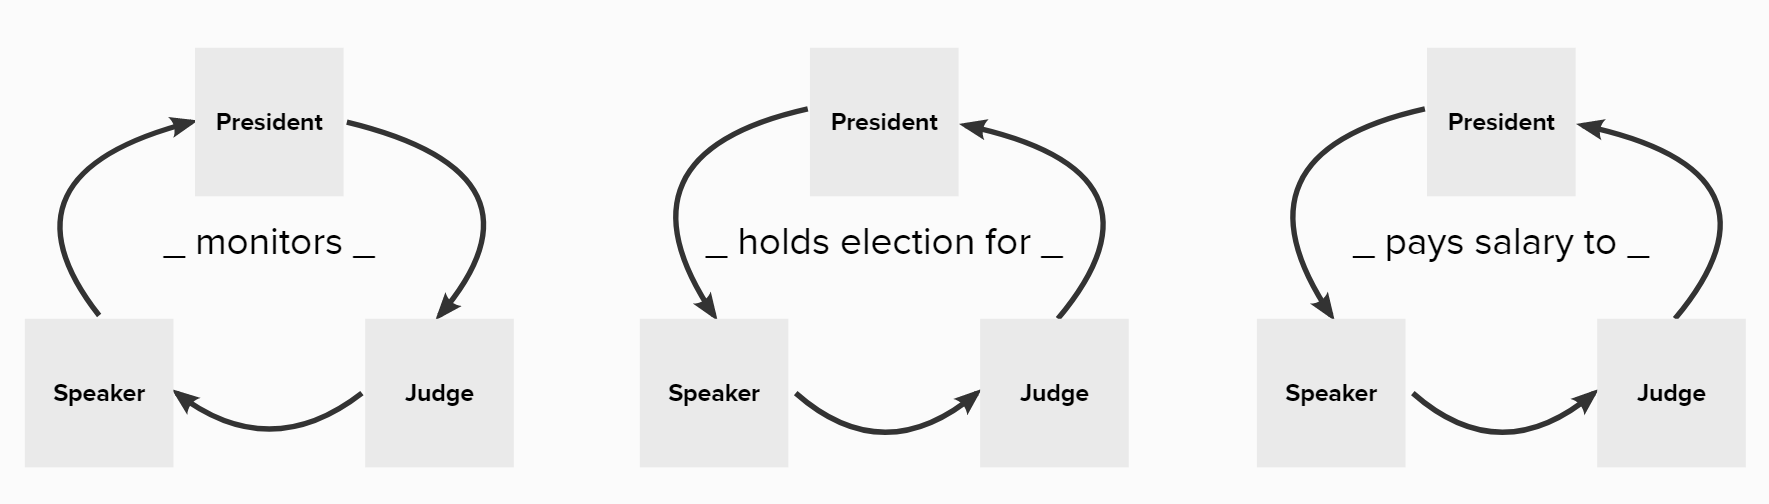
\includegraphics[scale=0.33]{05_iigo/images/role cycles.png}
\caption{Accountability cycle (left), the transfer-of-power cycle (middle) and salary cycle (right).}
\label{fig:cycles_in_IIGO}
\end{figure}


\subsection{Transfer-of-power}
\label{subsec:transfer-of-power}
\begin{enumerate}
    \item The Speaker conducts a vote for the election of the new Judge.
    \item The Judge conducts a vote for the election of the new President.
    \item The President conducts a vote for the election of the new Speaker.
\end{enumerate}
Refer to the Figure~ \ref{fig:cycles_in_IIGO} for further clarification about the transfer-of-power cycle.

\begin{rule_IIGO}
   The role $X$ has the \emph{obligation} to conduct a vote for the election of $Y$ at the end of the term (see Definition~\ref{def:term}) if and only if the role $X$ is accountable to the role $Y$. 
\end{rule_IIGO}.

\section{Budget and Salary}
\subsection{Budget}
%Actions associated with the IIGO have an associated cost that is defined as a configuration parameter. The institutional-power-enabled actions of  identified to require a "computational" component are:

Institutional-enabled-power actions in the IIGO have an associated cost with them. Some examples for such actions include:


%that is defined as a configuration parameter. The institutional-power-enabled actions of  identified to require a "computational" component are:


%We have defined the resource to be an endogenous one, hence any computation surrounding the distribution of the resource must use up some of that resource. 
\begin{itemize}
\item Calling any vote and computing the winner.
\item Declaring (e.g. \textit{announcing} the result of a vote).
\item Setting the amount of \emph{taxation} for each island.
\item Deciding the allocation distribution for each island.
\item Inspecting an island's action history.
\item Monitoring a role.
\end{itemize}

Since IIGO has been designed to act in the common good, IIGO-related costs will be directly withdrawn from the common pool. Since the common pool is considered a communal property of the archipelago, there are rules in place to limit how much each role is allowed to spend in order to perform its own institutional-power-enabled actions. This is the reason why defining the \emph{budget} and keeping it separate for each of the three IIGO roles.


As a role performs institutional-enabled-power actions, the corresponding cost associated with this action is subtracted from the role's budget. A budget of zero means that the role does not have the \emph{power} to perform any of its institutional-power-enabled actions. The removal of the budget rule from the rules in play means the role is allowed to perform as many such actions as it prefers to (as long as those actions are not governed by other rules). 



%As a role performs an endogenous-cost action, the corresponding cost associated with this action is subtracted from the role's budget. Thus, if as a result of an endogenous-cost action a role will be left with negative budget, it will have gone over the budget limit and will have broken the budget rule. A budget of zero means that the role is not allowed to perform any of its institutional-power-enabled actions associated an endogenous-cost. The removal of the budget rule from the rules in play means the role is allowed to perform as many such actions as it pleases (as long as those actions are not governed by other rules). 

The budget rule is also persistent across turns. This means that, assuming nothing else affects the budget, if a role has $100$ resources in its budget at each turn and spends only $10$ resources, this means that this very same role has $90$ resources in its budget at the next turn. On the other hand, islands can choose to increase the budget periodically every turn. This is governed by another budget extension rule.




%one turn and it spends 10, it has 90 resources in it's budget the next turn. 

Finally, it must be noted that the budget is inherently linked with the fact that whether obligations of a specific role can be undergone.
For example, during \emph{monitoring}, it should not be seen as a rule violation if a role has not acted on an obligation if it would go over the budget as a result. 

%This can also be seen as an added clause "... and the action is only permitted if they have the budget" to most rules which govern actions with an endogenous-cost.
%\begin{rule_IIGO}
    %The budget is increased by an amount $N$ every turn.
%\end{rule_IIGO}

%This rule means that, assuming nothing else affects the budget, if a budget is set to increase by 10 resources every turn and the budget is a 100 resources in turn one, the budget is 110 resources in turn 2. Setting this rule to 0 is equal to removing this rule and it means that the budget is never increased. 


\subsection{Salary}
\label{subsec:salary}
A salary is paid to each role in power as an incentive to act in a publicly approved way. %Hence, each role has the \emph{power} to pay a salary to another role following the salary cycle in Figure~\ref{fig:cycles_in_IIGO}.
\begin{rule_IIGO} \label{rule:salary}
   %Each role has the \emph{obligation} to pay the salary of amount $S$ to another if and only if the amount paid $S'$ is equal to $S$.
   Each role has the \emph{obligation} to pay the salary of amount $S$ to one another following the salary cycle in Figure~\ref{fig:cycles_in_IIGO}.
\end{rule_IIGO}

In Rule~\ref{rule:salary}, setting $S=0$ (through changing the active rules in place) means that roles do not have the permission to pay any salary. Removing the Rule~\ref{rule:salary} means that the roles may freely choose the amount $S$ for the salary payments.

\section{IIGO Session order}

\begin{enumerate}
    \item The Judge has the \emph{power} to check the history of actions to confirm whether the previously punished island(s) has/have obeyed the previous round's sanctions, meaning whether they contributed to the common pool accordingly in case of economic sanctions.
    %\begin{itemize}
      %  \item \emph{Suggested Rule:} In case of disobeying sanctions, the Judge is \emph{obliged} and \emph{permitted} to increase the severity of sanctions with respect to specific islands.
   % \end{itemize}
    \item The Judge has the \emph{power} to carry out \emph{inspections} on the history of actions of any island $X$ to check whether:
        \begin{enumerate}
        \item the reported resources of $X$ in the previous round match the real value of resources $X$ had in its private pool for the previous turn.
        \item the island $X$ has retrieved the right amount of the resources from the common pool, based on the \emph{allocation request} evaluated by the previous President.
            \begin{itemize}
            \item An example: In the previous round, the President has decided that the island $X$ can take $Y$ amount of resources from the common pool. If the Judge finds out that the island $X$ has taken an amount of $Y'$ such that $Y' > Y$, the Judge has the \emph{power} to invoke sanctions on the island $X$.
            
            %the Judge is \emph{obliged} and \emph{permitted} to sanction island $X$.
            \end{itemize}
        \end{enumerate}
    \item The Judge has the \emph{power} to invoke sanctions based on the outcome of the inspections.
    \item The President has the \emph{power} to decide to carry out a \emph{monitoring} on:
        \begin{enumerate}
        \item the sanctions imposed by the Judge.
        \end{enumerate}
    \item The islands may report the resources in their private pools to the President.
    \item The President has the \emph{power} to let each island know about the amount of \emph{taxation} they have to pay.
    \item The island has the \emph{power} to make an \emph{allocation request} to the President.
    \item The President has the \emph{power} decide on an allocation of resources and let each island know about the amount of resource allocation they are permitted to take from the common pool.
    \item The island has the \emph{power} to pick and to propose a rule to be voted on to the President.
    \item The President has the \emph{power} to choose a rule to be voted on from the received rule proposals.
    \item The Speaker has the \emph{power} to decide to carry out a \emph{monitoring} on: 
        \begin{enumerate}
        \item the resource allocation decided by the President.
        \item the rule proposed by the President.
        \end{enumerate}
    \item The Speaker has the \emph{power} to call a vote.
        \begin{enumerate}
        \item The islands vote in support of, or against, the rule (aye or nay) anonymously.
        \end{enumerate}
    \item The Speaker has the \emph{power} to announce a result of a vote to the islands and carries out the law change, if required (e.g. deleting/rejecting a rule if there is a majority nay vote).
    \item The Judge has the \emph{power} to decide to carry out \emph{monitoring} on:
        \begin{enumerate}
        \item the vote called by the Speaker.
        \item the Speaker announcing the result.
    \end{enumerate}
    \item The roles pay salary for one another following the accountability cycle in Figure~ \ref{fig:cycles_in_IIGO}.

\end{enumerate}



\section{Future Work}

\begin{itemize}
    \item \textbf{Diplomatic sanctions}: Although having the potential of being a good alternative for severer sanctions discussed in  Section~\ref{sec:sanctions}, diplomatic sanctions are \emph{not} implemented within the scope of the coursework. \\
    Suggested diplomatic sanctions include:
        \begin{itemize}
            \item Revoking an island's eligibility to vote and to be elected for a position.
            \item Revoking an island's eligibility to propose a rule/motion.
        \end{itemize}
    \item \textbf{Immutable rules}: Within the scope of the coursework, a subset of rules could have been categorised as immutable. This means that to change such immutable rules, the islands first need to vote to change their status to be \emph{mutable}, and consequently, hold another vote to change these mutable rules.
    %\item \textbf{Adding rules to the proposal list: } 
\end{itemize}

    
    % \input{00_example/example.tex}
    % \input{01_introduction/introduction.tex}
    % \documentclass[a4paper, twoside]{report}
% Template author: Y. Panagis

\usepackage[english]{babel}
\usepackage[utf8x]{inputenc}
\usepackage[T1]{fontenc}
\usepackage{listings}
\usepackage{hyperref}
\hypersetup{colorlinks=false}
\usepackage{lscape}
\usepackage{subfigure}
\usepackage{amsmath}
\usepackage{graphicx}
\usepackage[colorinlistoftodos]{todonotes}
\usepackage[ruled, vlined]{algorithm2e}
\usepackage{verbatim}
\usepackage{float}
\usepackage{tikz}
%\usepackage{algpseudocode}
\usepackage{tabularx}
%\usepackage{multirow}
\def\checkmark{\tikz\fill[scale=0.4](0,.35) -- (.25,0) -- (1,.7) -- (.25,.15) -- cycle;}

\newtheorem{definition}{Definition}

%% Sets page size and margins
\usepackage[a4paper,top=3cm,bottom=2cm,left=3cm,right=3cm,marginparwidth=2cm]{geometry}

\begin{document}
    % The Title, Author Name, Date, and abstract go here
    \title{Self-Organising Multi-Agent Systems: MVP Specifications}
    \author{SOMAS Class 2020-2021}
    \date{\today}
    \maketitle

    \tableofcontents    
    % if you are adding a new chapter, create a new folder in the root directory of the project
    % it should begin with a two digit number, followed by an underscore and the name of the section.
    % This keeps the order of the sections in the side view in keeping with the order of the document.
    
    \chapter{Inter-Island Governmental Organisation (IIGO)}


The role of IIGO is to maintain, update, and revise the rules concerning provision to managing the long-term collective risk dilemma (ltCRD). 

\begin{itemize}
    \item There will be 3 distinct branches in the IIGO: the \textbf{legislative branch}, \textbf{executive branch} and \textbf{judicial branch}\footnote{This is, as no surprise, inspired by the separation of powers in Western democracies.}.
    \item Each role is put in power according to the  transfer-of-power rules (see Section~\ref{subsec:transfer-of-power} for more detail).
    \item The head of the legislative branch is the Speaker, the head of the executive branch is the President, and the head of judicial branch is the Judge.
    \begin{itemize}
        \item  The Speaker, President and Judge are selected, through a democratic election, from the islands in the archipelago\footnote{This naming is inspired by the roles in the US Government.}.
        \item The resources gathered by the archipelago are endogenous, hence acting on the institutional powers granted to the Speaker, President or Judge costs resources. 
        \item For their duty, the President, the Speaker and the Judge receive a salary for each of their turns in office (see Section~\ref{subsec:salary} for more detail).
        \item The limit of the powers of the President, Speaker and Judge are defined in this chapter (e.g. the Speaker can only call one vote per turn).
 
    \end{itemize}
\end{itemize}

\subsection{IIGO Specific Definitions}
\begin{definition} \label{def:ballot}
    A \textbf{ballot} is related to each island's \textbf{power} to support or disagree with the rule specified in the vote called by the President and to vote in favour or against an island for a specific role (i.e. the President, Speaker, Judge) at each round of the game.
\end{definition}


%\begin{definition} \label{def:vote}
    %A \textbf{vote} is related to a role's (i.e. the President, Speaker, Judge) \textbf{power} to call a vote for a specific rule or an election.
%\end{definition}


\begin{definition} \label{def:tax}
    The \textbf{taxation} is related to the President's \textbf{power} to request a specific \underline{\textbf{minimum}} amount of contribution from each island to the common pool at each round of the game. 
\end{definition}

\begin{definition} \label{def:alloc_req}
    An \textbf{allocation request} is related to each island's \textbf{power} to request a specific amount of resource allocation from the President at each round of the game.
\end{definition}


\begin{definition} \label{def:rule_prop_list}
A \textbf{rule proposal list} is related to each island's \textbf{power} to propose a specific rule to be passed to the President at each round of the game.
\end{definition}

\begin{definition} \label{def:invst}
    An \textbf{investigation} is related to the Judge's \textbf{power} to acquire information to make a decision, followed by a calculation of the expected results and checking whether some specific rules have been obeyed, exclusively for the actions carried out by the \textbf{islands}. 
\end{definition}


An example of an \emph{investigation}: The President has permitted the island $X$ to take the amount of $Y$ resources from the common pool. Upon \emph{investigation} carried out by the Judge, it is revealed that the amount of resources taken out from the common pool by the island $X$ is, in fact, $Y'$ such that $Y' \neq Y$.


\begin{definition}
\textbf{Monitoring} is a government official's \textbf{power} to perform event recognition and to check whether some specific rules have been obeyed.
\end{definition}

An example of \emph{monitoring}: The Speaker has performed only the following action: \emph{counted the votes and calculated the result} for a rule. Upon \emph{monitoring} carried out by the President, it is noticed that the Speaker has not made any \emph{announcement}. Hence, the Speaker has not followed their obligation to \emph{announce} the result of any vote held.

See Section~\ref{sec:accountability} for more information about which roles can monitor which ones.


\begin{definition}
\textbf{Investigative-monitoring} is a government official's \textbf{power} to acquire the information used in acting on a governmental power followed by calculation of the expected results and checking whether some specific rules have been obeyed, exclusively for the actions carried out by a government official they are responsible for.
\end{definition}

An example of \emph{investigative-monitoring}: The Speaker has performed the following actions: \emph{counted the votes and calculated the result $R$} for a vote $V$ and \emph{announced} the result $R'$ for the vote $V$. Upon \emph{investigative-monitoring} carried out by the President, it is noticed that $R' \neq R$. Hence, the Speaker has modified the announced result.


\begin{definition}
The \textbf{sanction} is related to the Judge's \emph{power} to punish non-compliant islands when their disobedience is confirmed through investigations at a specific turn.
\end{definition}


\begin{definition}
The (judicial) \textbf{pardon} is related to the Judge's \emph{power} to forgive a non-compliant island at a specific turn.
\end{definition}

\begin{definition}
The \textbf{budget} is the maximum amount of resources a role is permitted to spend from the common pool as it performs its own institutional-power-enabled actions at a specific turn.
\end{definition}


\begin{definition}
The \textbf{salary} is the amount of resources a role is to be given from the common pool as a reward for performing its institutional-power-enabled actions at a specific turn.
\end{definition}

\begin{definition} \label{def:term}
A \textbf{term} is the number of turns an island is \emph{permitted} to hold a role, and after which the responsible role (indicated in the transfer-of-power cycle in Figure~\ref{fig:cycles_in_IIGO}) is \emph{obliged} to initiate transfer-of-power.
\end{definition}

\subsection{\emph{Power}, \emph{Permission} and \emph{Obligation} Distinction}
In the rest of the specifications, we will be specifically using the following three terms to define the actions and responsibilities carried out by the Speaker, President, Judge (see Figure~ \ref{fig:per_obl_sets}):
\begin{itemize}
    \item Power
    \item Permission
    \item Obligation
\end{itemize}



\begin{figure}[H] 
\centering
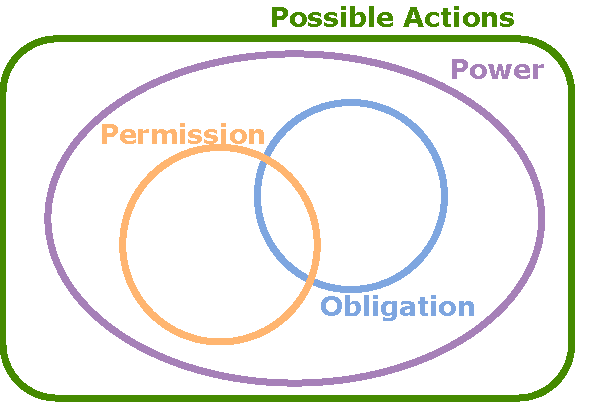
\includegraphics[width=0.6\textwidth]{05_iigo/images/SOMAS_per_obl.pdf}
\caption{Relationship between \emph{power}, \emph{permission} and \emph{obligation}.}
\label{fig:per_obl_sets}
\end{figure} 


For example, the Judge has the \emph{power} to carry out investigations at an IIGO session. There are no rules specifying which specific islands the Judge should investigate. Therefore, the Judge has the \emph{permission} to investigate any `alive' islands during a session. However, the Judge is \emph{obliged} to make at least some number of investigations each turn.



\section{Executive Branch}
\label{sec:executive}
The executive branch is responsible for \textbf{carrying out the law}.
\begin{itemize}
       
    \item The President has the \emph{power} to: 
    \begin{itemize}
        
        \item Select a rule for voting $R^{*}$ to be passed to the Speaker.
        \begin{rule_IIGO}
            The President has the \emph{obligation} to \emph{select} a rule $R^{*}$ if the \emph{rule proposal list} has at least one proposed rule in it.
        \end{rule_IIGO}
        \begin{rule_IIGO}
            The President has the \emph{permission} to \emph{select} a rule $R^{*}$ if and only if $R^{*} \in S$, where $S$ is the \emph{rule proposal list}.
        \end{rule_IIGO}
        
        \item Decide the amount of individual \emph{taxation} (i.e. a specific \emph{minimum} amount of contribution to the common pool for each island) for the current turn.
        
        \begin{itemize}
            \item The President is given the self-reported resource amounts held by each island to assist in this decision.
            %\item Suggested Rule: For any island that has chosen to not report it's resources, the President has the \emph{obligation} to set them an individual tax amount T.
        \end{itemize}
        
        \item Decide the allocation of resources distributed from the common pool to the islands (i.e. a specific \emph{maximum} amount an island is permitted to take from the common pool).
        
        \begin{itemize}
            \item The President is given the \emph{allocation requests} made by each island.
            %\item \emph{}{Suggested Rule:} The President has an obligation to prioritise islands in critical condition.
        \end{itemize}
    \end{itemize}
\end{itemize}



\section{Legislative Branch}
\label{sec:legislative}
The legislative branch is responsible for \textbf{making the law}.
\begin{itemize}

    \item The Speaker has the \emph{power} to:
    \begin{itemize}
        
        \item Call a vote $V$ for a rule $R$.
        \begin{rule_IIGO}
            The Speaker has the \emph{obligation} to \emph{call} a vote $V$ if and only if the President has \emph{selected} a rule $R$ to be voted on.
        \end {rule_IIGO}
        \begin{rule_IIGO}
            The Speaker has the \emph{permission} to \emph{call} a vote $V$ for a rule $R$ if and only if the rule $R = R^{*}$, where $R^{*}$ is the rule \emph{selected} by the President.
        \end {rule_IIGO}
            
        \item Choose which islands are participating in the vote $V$.
       % \footnote{This is our sequential implementation alternative for the power to close the ballot box.}.
        \begin{rule_IIGO}
            The Speaker has the \emph{obligation} to ask for a vote from all alive islands.
        \end {rule_IIGO}
            
        \item Declare the result $C$ of a vote $V$. 
        \begin{rule_IIGO}
            The Speaker has the \emph{obligation} to \emph{declare the result} $C$ for a vote $V$ if and only if the vote V has been \emph{called}.
        \end {rule_IIGO}
        \begin{rule_IIGO}
            The Speaker has the \emph{permission} to \emph{declare the result} $C$ for a vote $V$ if $C = C^{*}$, where $C^{*}$ is the result produced by \emph{calling} the vote $V$.
        \end {rule_IIGO}
        \begin{itemize}
            \item This step is what enables a rule to be \emph{active}.
        \end{itemize}
    \end{itemize}
\end{itemize}




\section{Judicial Branch}
\label{sec:judicial}

The judicial branch is responsible for \textbf{evaluating the law}.
\begin{itemize}
    \item The Judge has the \emph{power} to:
    \begin{itemize}
        \item Perform a number of \emph{inspections}\footnote{An \emph{inspection} \textbf{costs} an expense of resources (See Definition~\ref{def:invst} for more detail).} $I$ and produce a compliance outcome $\mathbb{O}^{*}$\footnote{Note that the compliance outcome $\mathbb{O}^{*}$ considered is a boolean.}.
        %(true: the island has been compliant with the rules in play, false: the island has not been compliant with the rules in play)
        %\begin{itemize}
           % \item For example, to check if the event outcome is \emph{concurrent}\footnote{Again, what is defined as "concurrent"? A clear definition is needed.} with the rules.
        %\end{itemize}
        \begin{rule_IIGO}
            The Judge has the \emph{obligation} to make at least $N$ investigations at each turn.
        \end{rule_IIGO}
        \item Declare the outcome $\mathbb{O}$ of an inspection $I$ to all islands\footnote{This act of broadcasting is especially important for islands to form an opinion about the sanctioned islands accordingly.}.
        \begin{rule_IIGO}
            The Judge has the \emph{obligation} to declare the outcome $\mathbb{O}$ of an inspection $I$ if and only if the inspection $I$ has been performed.
        \end{rule_IIGO}
        \begin{rule_IIGO}
            The Judge has the \emph{permission} to declare the outcome $\mathbb{O}$ of an inspection $I$ if $\mathbb{O} = \mathbb{O}^{*}$, where $\mathbb{O}^{*}$ is the outcome of the inspection $I$.
        \end{rule_IIGO}
        %\item Initiate the removal of the \texttt{President}.
        %\begin{itemize}
            %\item A good Judge would be especially vigilant during \emph{power transfer} regarding the \emph{President} position (see Section~\ref{leg_const} for more detail).
        %\end{itemize}
        \item Invoke economic \textbf{sanctions} (see Section~\ref{sec:sanctions} for more detail).
        \begin{rule_IIGO}
            The Judge has the \emph{obligation} to invoke a sanction $S$ for an island $X$ if and only if an investigation $I$ has an outcome $\mathbb{O}^{*}$ indicating non-compliance, and $I$ is an investigation of an action taken by island $X$.
        \end{rule_IIGO}
        \item Invoke even more severe sanctions in the case of further disobedience to previous sanction(s).
        \begin{rule_IIGO}
            The Judge has the \emph{permission} to invoke a severer sanction $S'$ for an island $X$ if the island $X$ has not fulfilled the requirements of the previous sanction $S$.
        \end{rule_IIGO}
        \item Pardon the islands which are currently sanctioned.
        \begin{rule_IIGO}
            The Judge has the \emph{permission} to revoke any sanction $S$ of an island $X$ at a specific turn.
        \end{rule_IIGO}
    \end{itemize}
\end{itemize}
%(e.g. a new rule that falls under a "sanction" category \hl{[I'm not sure about this being a `new rule` [Ezgi]]}

\subsection{Sanctions}
\label{sec:sanctions}
All sanctions are of economic nature which include:
        \begin{itemize}
            %\item Revoking an island's access to the common pool.
            \item Enforcing an island to contribute a specific amount of resources to the common pool.
            \begin{itemize}
                \item This does not mean that the Judge has the \emph{power} to take resources from an island in order to put them to the common pool -- the island itself is expected to carry out this implication imposed by the sanction itself, otherwise further punishment can be induced by the Judge.
                \item Similarly, \emph{opinion formulation} will follow accordingly whether the island(s) is/are following the implications imposed by the sanction(s).
            \end{itemize}
        
    \end{itemize}
    Sanctions are the associated penalty that comes with an island breaking a specific rule. The Judge is in full control of the penalties associated with breaking any rules. Once the Judge has specified the score of the penalty associated with each time an island breaks a rule, the cumulative penalties accumulated by the island are then used to determine which \textbf{sanction tier} that each island falls into. The score threshold to determine the boundaries of the sanction tiers are set by the Judge. At each turn of the game, each island is told whether they are being sanctioned, and if so, which \textbf{sanction tier} that they are currently in. The \textbf{sanction tiers} of the non-compliant islands are also broadcasted to the other islands in the archipelago. To summarise, the sanctioning process follows these steps:
    
    
    
    %Sanctions are based on an island breaking a rule. Each rule must therefore have an associated penalty. By default, we set these penalties such that they add $1$ to the total sanction score for each island. However, we allow the judge to override this scoring, the judge is able to set their own scores for any particular rule as they desire. This custom scoring is then used when an island breaks a particular rule. By looking at events that occurred in the last turn, and using the customised scoring we provide the holder of the judge role with full control of the penalties for breaking any rules.
    
    





%we then use the cumulative penalties accumulated by each island to determine which Sanction Tier they fall into. The score threshold's required to fall into these sanction tiers is set by the judge and is checked for monotonicity. Each island is told whether they are being sanctioned, and is so what tier they are in. We also tell other islands about which sanction tiers other islands have fallen into. 

    \begin{enumerate}
        \item The Judge has the \emph{power} to set custom penalties associated with breaking any rules.
        \item The Judge is given a list of all events that occurred in the previous turn.
        \item The Judge has the \emph{power} to check whether any, or all of these previous events, involve the islands in the archipelago breaking any rules.
        \item Each of the transgressions is scored using the Judge's custom penalties if the Judge has set them. Otherwise, a score of $1$ is given each time a rule is broken.
        \item The Judge has the \emph{power} to revise the sanction thresholds.
        \item Using the latest sanction thresholds available, each island is assigned to a sanction tier based on the sanction score that it has received.
        \item These sanction tiers are broadcasted to all of the islands in the archipelago.
        \item The Judge then uses sanctions rules in place to calculate the specific amount of resources that each non-compliant island has in order to determine how much it should contribute to the common pool, based on the sanction tier that it is in.
    \end{enumerate}



\section{Constitutional Rights and Obligations in the Archipelago}
\label{sec:const_rights_obl_archi}
Each island has the \emph{power} to:
\begin{itemize}
\item make an \emph{allocation request} (see Definition~\ref{def:alloc_req}) to the President for a specific amount to be allocated to them.
\item report the number of resources it is in possession of to the President.
\begin{rule_IIGO}
    Each island has the \emph{obligation} to report the number of resources it is in possession of to the President.
\end{rule_IIGO}
\begin{rule_IIGO}
    Each island has the \emph{permission} to report the number of resources $R'$ if and only if $R' = R$, where R is the number of resources the island is in possession of.
\end{rule_IIGO}
\item take resources from the common pool.


\begin{rule_IIGO}
    Each island has the \emph{permission} to take at maximum $N$ resources, where $N$ is the specific allocation made by the President to that island\footnote{If no such allocation is made, the island is \emph{permitted} to take any amount of resources.}.
\end{rule_IIGO}
\item contribute resources to the common pool.
\begin{rule_IIGO}
    Each island has the \emph{obligation} to contribute to the common pool an amount greater or equal to that of the individual tax set by the President.
\end{rule_IIGO}
                %The President is in
                %(unless there is a rule in place that dictates how Speaker is to allocate resources).
\item add a rule to the \emph{rule proposal list} (see Definition~\ref{def:rule_prop_list}) at the start of each turn.
        %\begin{itemize}
            %\item The game specification includes how many rules an island can propose each turn.
        %\end{itemize}
        %\item vote  for rules in the Legislative Branch and vote for their favourite islands in elections
\item participate in the legislative branch of the government by casting ballots in votes called by the Speaker
\item vote for an island to be elected for a specific role (e.g. the President, Judge, Speaker) during the elections\footnote{This will be assumed to be true \underline{unless stated otherwise}. %Note that \textbf{diplomatic sanctions} can disable this power of a specific island (see Section~\ref{jud_const}).}.
        }.
\end{itemize}
\section{Accountability Cycle}
\label{sec:accountability}


To ensure that the government avoids corruption and abuse of power, each branch is accountable to another. The President is accountable to the Speaker, the Speaker is accountable to the Judge, and the Judge is accountable to the President (see Figure~ \ref{fig:cycles_in_IIGO}). This accountability cycle is enacted through \emph{monitoring} actions\footnote{Note that the terms \textbf{monitoring} and \textbf{investigation} have similar but quite different meanings in the IIGO context.}. 

The powers related to the accountability cycle and transfer-of-power for each role can be summarized as the following: 
\begin{itemize}
    \item The Speaker has the \emph{power} to: 
    \begin{itemize}
        \item monitor the President.
        \item announce the result of this monitoring.
        \item initiate the transfer-of-power for the Judge.
    \end{itemize}
    \item The President has the \emph{power} to: 
    \begin{itemize}
        \item monitor the Judge.
        \item announce the result of this monitoring.
        \item initiate the transfer-of-power for the Speaker.
    \end{itemize}
    \item The Judge has the \emph{power} to: 
    \begin{itemize}
        \item  monitor the Speaker.
        \item announce the result of this monitoring.
        \item initiate the transfer-of-power for the President.
    \end{itemize}
\end{itemize}

%Unlike investigations performed by the Judge, who performs investigations on island actions in the following turn, each role is given the opportunity to check up on the actions of the role it is responsible for immediately after they have been performed. In this sense, the President can monitor (includes investigative-monitoring) the powers (calling a vote and announcing the result) acted on by the Speaker immediately after the Speaker's announcement (or lack there of). The government officials hold a lot of power so this is to ensure that any wrong-doing is determined as quickly as possible. For this project we are only pursuing one degree of monitoring, that is, the powers relating to the accountability cycle will not be monitored themselves. We assume that agents will act in the interest of themselves and keeping all the islands alive is beneficial to everyone. Hence, while the agents might be inclined to break rules in order to benefit themselves, anyone else breaking the rules is seen as undesirable under the assumption that the system in place is there to benefit all. 


Through the proposed accountability cycle, each role is given the opportunity to check up on the actions of the role it is accountable for immediately after they have been performed. It is clear that the IIGO roles (i.e. the President, Speaker and Judge) hold a considerable amount of \emph{power} in their hands. The accountability cycle is designed to address the possible abuses of this power. With monitoring, any wrong-doing in the IGO is determined as quickly as possible and the role in question can be replaced. 

Within the scope of the coursework, we decided to pursue only \emph{one degree of monitoring}, meaning that the powers relating to the accountability cycle will not be monitored themselves. We assume that agents will act in the interest of all the islands in the archipelago. Hence, while the agents might be inclined to break the rules to benefit in some form, it is assumed that the others will negatively see any non-compliant islands based on the assumption that the proposed IIGO system is in place to maintain the welfare of all the islands.

Let role $X$ be accountable to the role $Y$, which is accountable to the role $Z$. Then:
\begin{rule_IIGO}
$Y$ has the \emph{obligation} to declare the outcome of the monitoring result $M$ associated with the action $A$ undertaken by $X$ if and only if $Y$ has monitored the action $A$ performed by $X$. 
\end{rule_IIGO}
\begin{rule_IIGO}
$Y$ has the \emph{permission} to declare the monitoring result $M$ associated with the action $A$ undertaken by $X$ if and only if $M = M^{*}$, where $M^{*}$ is the outcome of \emph{monitoring} action $A$ performed by $X$\footnote{These constitutional rules should be available to the agents to check their decision against. However, due to having only one degree of accountability cycle in place, these rules are not enforced through any sanctions (i.e. breaking these rules has no consequences as they only deem to be an \emph{agreement} among the roles).}.
\end{rule_IIGO}


\begin{figure}[!htb]
\centering
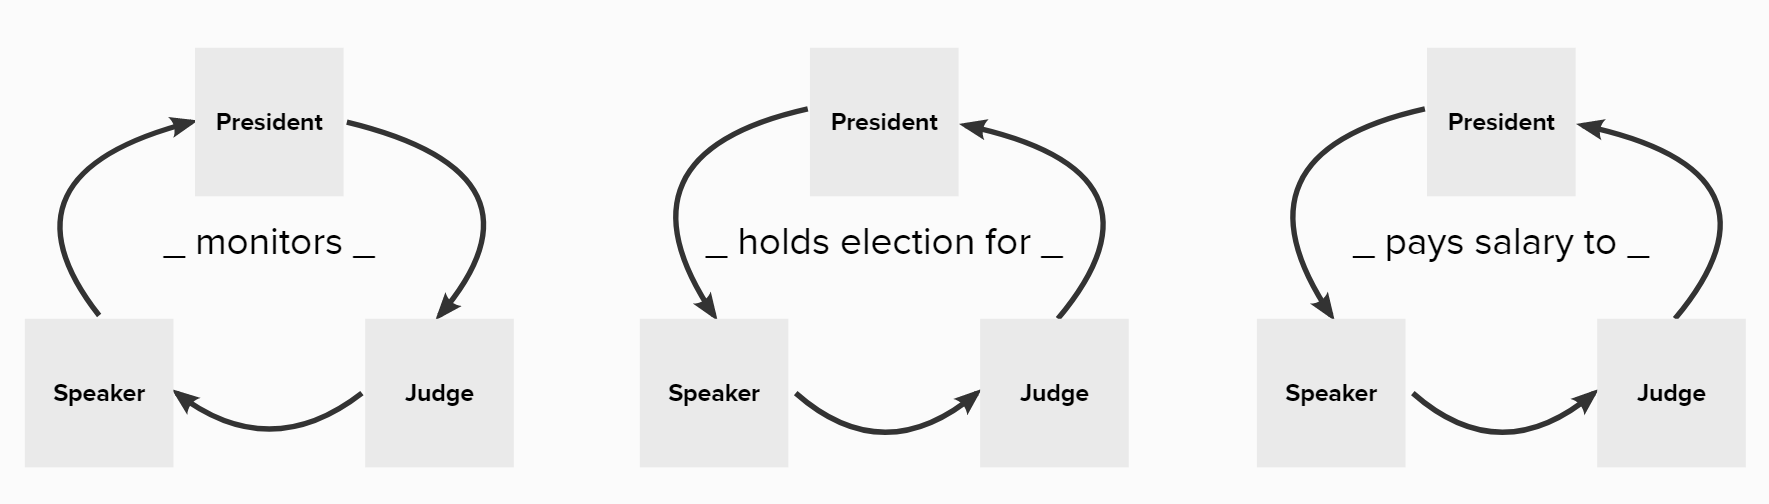
\includegraphics[scale=0.33]{05_iigo/images/role cycles.png}
\caption{Accountability cycle (left), the transfer-of-power cycle (middle) and salary cycle (right).}
\label{fig:cycles_in_IIGO}
\end{figure}


\subsection{Transfer-of-power}
\label{subsec:transfer-of-power}
\begin{enumerate}
    \item The Speaker conducts a vote for the election of the new Judge.
    \item The Judge conducts a vote for the election of the new President.
    \item The President conducts a vote for the election of the new Speaker.
\end{enumerate}
Refer to the Figure~ \ref{fig:cycles_in_IIGO} for further clarification about the transfer-of-power cycle.

\begin{rule_IIGO}
   The role $X$ has the \emph{obligation} to conduct a vote for the election of $Y$ at the end of the term (see Definition~\ref{def:term}) if and only if the role $X$ is accountable to the role $Y$. 
\end{rule_IIGO}.

\section{Budget and Salary}
\subsection{Budget}
%Actions associated with the IIGO have an associated cost that is defined as a configuration parameter. The institutional-power-enabled actions of  identified to require a "computational" component are:

Institutional-enabled-power actions in the IIGO have an associated cost with them. Some examples for such actions include:


%that is defined as a configuration parameter. The institutional-power-enabled actions of  identified to require a "computational" component are:


%We have defined the resource to be an endogenous one, hence any computation surrounding the distribution of the resource must use up some of that resource. 
\begin{itemize}
\item Calling any vote and computing the winner.
\item Declaring (e.g. \textit{announcing} the result of a vote).
\item Setting the amount of \emph{taxation} for each island.
\item Deciding the allocation distribution for each island.
\item Inspecting an island's action history.
\item Monitoring a role.
\end{itemize}

Since IIGO has been designed to act in the common good, IIGO-related costs will be directly withdrawn from the common pool. Since the common pool is considered a communal property of the archipelago, there are rules in place to limit how much each role is allowed to spend in order to perform its own institutional-power-enabled actions. This is the reason why defining the \emph{budget} and keeping it separate for each of the three IIGO roles.


As a role performs institutional-enabled-power actions, the corresponding cost associated with this action is subtracted from the role's budget. A budget of zero means that the role does not have the \emph{power} to perform any of its institutional-power-enabled actions. The removal of the budget rule from the rules in play means the role is allowed to perform as many such actions as it prefers to (as long as those actions are not governed by other rules). 



%As a role performs an endogenous-cost action, the corresponding cost associated with this action is subtracted from the role's budget. Thus, if as a result of an endogenous-cost action a role will be left with negative budget, it will have gone over the budget limit and will have broken the budget rule. A budget of zero means that the role is not allowed to perform any of its institutional-power-enabled actions associated an endogenous-cost. The removal of the budget rule from the rules in play means the role is allowed to perform as many such actions as it pleases (as long as those actions are not governed by other rules). 

The budget rule is also persistent across turns. This means that, assuming nothing else affects the budget, if a role has $100$ resources in its budget at each turn and spends only $10$ resources, this means that this very same role has $90$ resources in its budget at the next turn. On the other hand, islands can choose to increase the budget periodically every turn. This is governed by another budget extension rule.




%one turn and it spends 10, it has 90 resources in it's budget the next turn. 

Finally, it must be noted that the budget is inherently linked with the fact that whether obligations of a specific role can be undergone.
For example, during \emph{monitoring}, it should not be seen as a rule violation if a role has not acted on an obligation if it would go over the budget as a result. 

%This can also be seen as an added clause "... and the action is only permitted if they have the budget" to most rules which govern actions with an endogenous-cost.
%\begin{rule_IIGO}
    %The budget is increased by an amount $N$ every turn.
%\end{rule_IIGO}

%This rule means that, assuming nothing else affects the budget, if a budget is set to increase by 10 resources every turn and the budget is a 100 resources in turn one, the budget is 110 resources in turn 2. Setting this rule to 0 is equal to removing this rule and it means that the budget is never increased. 


\subsection{Salary}
\label{subsec:salary}
A salary is paid to each role in power as an incentive to act in a publicly approved way. %Hence, each role has the \emph{power} to pay a salary to another role following the salary cycle in Figure~\ref{fig:cycles_in_IIGO}.
\begin{rule_IIGO} \label{rule:salary}
   %Each role has the \emph{obligation} to pay the salary of amount $S$ to another if and only if the amount paid $S'$ is equal to $S$.
   Each role has the \emph{obligation} to pay the salary of amount $S$ to one another following the salary cycle in Figure~\ref{fig:cycles_in_IIGO}.
\end{rule_IIGO}

In Rule~\ref{rule:salary}, setting $S=0$ (through changing the active rules in place) means that roles do not have the permission to pay any salary. Removing the Rule~\ref{rule:salary} means that the roles may freely choose the amount $S$ for the salary payments.

\section{IIGO Session order}

\begin{enumerate}
    \item The Judge has the \emph{power} to check the history of actions to confirm whether the previously punished island(s) has/have obeyed the previous round's sanctions, meaning whether they contributed to the common pool accordingly in case of economic sanctions.
    %\begin{itemize}
      %  \item \emph{Suggested Rule:} In case of disobeying sanctions, the Judge is \emph{obliged} and \emph{permitted} to increase the severity of sanctions with respect to specific islands.
   % \end{itemize}
    \item The Judge has the \emph{power} to carry out \emph{inspections} on the history of actions of any island $X$ to check whether:
        \begin{enumerate}
        \item the reported resources of $X$ in the previous round match the real value of resources $X$ had in its private pool for the previous turn.
        \item the island $X$ has retrieved the right amount of the resources from the common pool, based on the \emph{allocation request} evaluated by the previous President.
            \begin{itemize}
            \item An example: In the previous round, the President has decided that the island $X$ can take $Y$ amount of resources from the common pool. If the Judge finds out that the island $X$ has taken an amount of $Y'$ such that $Y' > Y$, the Judge has the \emph{power} to invoke sanctions on the island $X$.
            
            %the Judge is \emph{obliged} and \emph{permitted} to sanction island $X$.
            \end{itemize}
        \end{enumerate}
    \item The Judge has the \emph{power} to invoke sanctions based on the outcome of the inspections.
    \item The President has the \emph{power} to decide to carry out a \emph{monitoring} on:
        \begin{enumerate}
        \item the sanctions imposed by the Judge.
        \end{enumerate}
    \item The islands may report the resources in their private pools to the President.
    \item The President has the \emph{power} to let each island know about the amount of \emph{taxation} they have to pay.
    \item The island has the \emph{power} to make an \emph{allocation request} to the President.
    \item The President has the \emph{power} decide on an allocation of resources and let each island know about the amount of resource allocation they are permitted to take from the common pool.
    \item The island has the \emph{power} to pick and to propose a rule to be voted on to the President.
    \item The President has the \emph{power} to choose a rule to be voted on from the received rule proposals.
    \item The Speaker has the \emph{power} to decide to carry out a \emph{monitoring} on: 
        \begin{enumerate}
        \item the resource allocation decided by the President.
        \item the rule proposed by the President.
        \end{enumerate}
    \item The Speaker has the \emph{power} to call a vote.
        \begin{enumerate}
        \item The islands vote in support of, or against, the rule (aye or nay) anonymously.
        \end{enumerate}
    \item The Speaker has the \emph{power} to announce a result of a vote to the islands and carries out the law change, if required (e.g. deleting/rejecting a rule if there is a majority nay vote).
    \item The Judge has the \emph{power} to decide to carry out \emph{monitoring} on:
        \begin{enumerate}
        \item the vote called by the Speaker.
        \item the Speaker announcing the result.
    \end{enumerate}
    \item The roles pay salary for one another following the accountability cycle in Figure~ \ref{fig:cycles_in_IIGO}.

\end{enumerate}



\section{Future Work}

\begin{itemize}
    \item \textbf{Diplomatic sanctions}: Although having the potential of being a good alternative for severer sanctions discussed in  Section~\ref{sec:sanctions}, diplomatic sanctions are \emph{not} implemented within the scope of the coursework. \\
    Suggested diplomatic sanctions include:
        \begin{itemize}
            \item Revoking an island's eligibility to vote and to be elected for a position.
            \item Revoking an island's eligibility to propose a rule/motion.
        \end{itemize}
    \item \textbf{Immutable rules}: Within the scope of the coursework, a subset of rules could have been categorised as immutable. This means that to change such immutable rules, the islands first need to vote to change their status to be \emph{mutable}, and consequently, hold another vote to change these mutable rules.
    %\item \textbf{Adding rules to the proposal list: } 
\end{itemize}

    \chapter{Inter-Island Governmental Organisation (IIGO)}


The role of IIGO is to maintain, update, and revise the rules concerning provision to managing the long-term collective risk dilemma (ltCRD). 

\begin{itemize}
    \item There will be 3 distinct branches in the IIGO: the \textbf{legislative branch}, \textbf{executive branch} and \textbf{judicial branch}\footnote{This is, as no surprise, inspired by the separation of powers in Western democracies.}.
    \item Each role is put in power according to the  transfer-of-power rules (see Section~\ref{subsec:transfer-of-power} for more detail).
    \item The head of the legislative branch is the Speaker, the head of the executive branch is the President, and the head of judicial branch is the Judge.
    \begin{itemize}
        \item  The Speaker, President and Judge are selected, through a democratic election, from the islands in the archipelago\footnote{This naming is inspired by the roles in the US Government.}.
        \item The resources gathered by the archipelago are endogenous, hence acting on the institutional powers granted to the Speaker, President or Judge costs resources. 
        \item For their duty, the President, the Speaker and the Judge receive a salary for each of their turns in office (see Section~\ref{subsec:salary} for more detail).
        \item The limit of the powers of the President, Speaker and Judge are defined in this chapter (e.g. the Speaker can only call one vote per turn).
 
    \end{itemize}
\end{itemize}

\subsection{IIGO Specific Definitions}
\begin{definition} \label{def:ballot}
    A \textbf{ballot} is related to each island's \textbf{power} to support or disagree with the rule specified in the vote called by the President and to vote in favour or against an island for a specific role (i.e. the President, Speaker, Judge) at each round of the game.
\end{definition}


%\begin{definition} \label{def:vote}
    %A \textbf{vote} is related to a role's (i.e. the President, Speaker, Judge) \textbf{power} to call a vote for a specific rule or an election.
%\end{definition}


\begin{definition} \label{def:tax}
    The \textbf{taxation} is related to the President's \textbf{power} to request a specific \underline{\textbf{minimum}} amount of contribution from each island to the common pool at each round of the game. 
\end{definition}

\begin{definition} \label{def:alloc_req}
    An \textbf{allocation request} is related to each island's \textbf{power} to request a specific amount of resource allocation from the President at each round of the game.
\end{definition}


\begin{definition} \label{def:rule_prop_list}
A \textbf{rule proposal list} is related to each island's \textbf{power} to propose a specific rule to be passed to the President at each round of the game.
\end{definition}

\begin{definition} \label{def:invst}
    An \textbf{investigation} is related to the Judge's \textbf{power} to acquire information to make a decision, followed by a calculation of the expected results and checking whether some specific rules have been obeyed, exclusively for the actions carried out by the \textbf{islands}. 
\end{definition}


An example of an \emph{investigation}: The President has permitted the island $X$ to take the amount of $Y$ resources from the common pool. Upon \emph{investigation} carried out by the Judge, it is revealed that the amount of resources taken out from the common pool by the island $X$ is, in fact, $Y'$ such that $Y' \neq Y$.


\begin{definition}
\textbf{Monitoring} is a government official's \textbf{power} to perform event recognition and to check whether some specific rules have been obeyed.
\end{definition}

An example of \emph{monitoring}: The Speaker has performed only the following action: \emph{counted the votes and calculated the result} for a rule. Upon \emph{monitoring} carried out by the President, it is noticed that the Speaker has not made any \emph{announcement}. Hence, the Speaker has not followed their obligation to \emph{announce} the result of any vote held.

See Section~\ref{sec:accountability} for more information about which roles can monitor which ones.


\begin{definition}
\textbf{Investigative-monitoring} is a government official's \textbf{power} to acquire the information used in acting on a governmental power followed by calculation of the expected results and checking whether some specific rules have been obeyed, exclusively for the actions carried out by a government official they are responsible for.
\end{definition}

An example of \emph{investigative-monitoring}: The Speaker has performed the following actions: \emph{counted the votes and calculated the result $R$} for a vote $V$ and \emph{announced} the result $R'$ for the vote $V$. Upon \emph{investigative-monitoring} carried out by the President, it is noticed that $R' \neq R$. Hence, the Speaker has modified the announced result.


\begin{definition}
The \textbf{sanction} is related to the Judge's \emph{power} to punish non-compliant islands when their disobedience is confirmed through investigations at a specific turn.
\end{definition}


\begin{definition}
The (judicial) \textbf{pardon} is related to the Judge's \emph{power} to forgive a non-compliant island at a specific turn.
\end{definition}

\begin{definition}
The \textbf{budget} is the maximum amount of resources a role is permitted to spend from the common pool as it performs its own institutional-power-enabled actions at a specific turn.
\end{definition}


\begin{definition}
The \textbf{salary} is the amount of resources a role is to be given from the common pool as a reward for performing its institutional-power-enabled actions at a specific turn.
\end{definition}

\begin{definition} \label{def:term}
A \textbf{term} is the number of turns an island is \emph{permitted} to hold a role, and after which the responsible role (indicated in the transfer-of-power cycle in Figure~\ref{fig:cycles_in_IIGO}) is \emph{obliged} to initiate transfer-of-power.
\end{definition}

\subsection{\emph{Power}, \emph{Permission} and \emph{Obligation} Distinction}
In the rest of the specifications, we will be specifically using the following three terms to define the actions and responsibilities carried out by the Speaker, President, Judge (see Figure~ \ref{fig:per_obl_sets}):
\begin{itemize}
    \item Power
    \item Permission
    \item Obligation
\end{itemize}



\begin{figure}[H] 
\centering
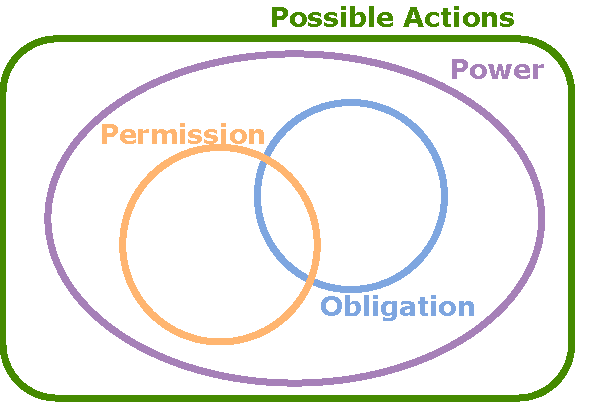
\includegraphics[width=0.6\textwidth]{05_iigo/images/SOMAS_per_obl.pdf}
\caption{Relationship between \emph{power}, \emph{permission} and \emph{obligation}.}
\label{fig:per_obl_sets}
\end{figure} 


For example, the Judge has the \emph{power} to carry out investigations at an IIGO session. There are no rules specifying which specific islands the Judge should investigate. Therefore, the Judge has the \emph{permission} to investigate any `alive' islands during a session. However, the Judge is \emph{obliged} to make at least some number of investigations each turn.



\section{Executive Branch}
\label{sec:executive}
The executive branch is responsible for \textbf{carrying out the law}.
\begin{itemize}
       
    \item The President has the \emph{power} to: 
    \begin{itemize}
        
        \item Select a rule for voting $R^{*}$ to be passed to the Speaker.
        \begin{rule_IIGO}
            The President has the \emph{obligation} to \emph{select} a rule $R^{*}$ if the \emph{rule proposal list} has at least one proposed rule in it.
        \end{rule_IIGO}
        \begin{rule_IIGO}
            The President has the \emph{permission} to \emph{select} a rule $R^{*}$ if and only if $R^{*} \in S$, where $S$ is the \emph{rule proposal list}.
        \end{rule_IIGO}
        
        \item Decide the amount of individual \emph{taxation} (i.e. a specific \emph{minimum} amount of contribution to the common pool for each island) for the current turn.
        
        \begin{itemize}
            \item The President is given the self-reported resource amounts held by each island to assist in this decision.
            %\item Suggested Rule: For any island that has chosen to not report it's resources, the President has the \emph{obligation} to set them an individual tax amount T.
        \end{itemize}
        
        \item Decide the allocation of resources distributed from the common pool to the islands (i.e. a specific \emph{maximum} amount an island is permitted to take from the common pool).
        
        \begin{itemize}
            \item The President is given the \emph{allocation requests} made by each island.
            %\item \emph{}{Suggested Rule:} The President has an obligation to prioritise islands in critical condition.
        \end{itemize}
    \end{itemize}
\end{itemize}



\section{Legislative Branch}
\label{sec:legislative}
The legislative branch is responsible for \textbf{making the law}.
\begin{itemize}

    \item The Speaker has the \emph{power} to:
    \begin{itemize}
        
        \item Call a vote $V$ for a rule $R$.
        \begin{rule_IIGO}
            The Speaker has the \emph{obligation} to \emph{call} a vote $V$ if and only if the President has \emph{selected} a rule $R$ to be voted on.
        \end {rule_IIGO}
        \begin{rule_IIGO}
            The Speaker has the \emph{permission} to \emph{call} a vote $V$ for a rule $R$ if and only if the rule $R = R^{*}$, where $R^{*}$ is the rule \emph{selected} by the President.
        \end {rule_IIGO}
            
        \item Choose which islands are participating in the vote $V$.
       % \footnote{This is our sequential implementation alternative for the power to close the ballot box.}.
        \begin{rule_IIGO}
            The Speaker has the \emph{obligation} to ask for a vote from all alive islands.
        \end {rule_IIGO}
            
        \item Declare the result $C$ of a vote $V$. 
        \begin{rule_IIGO}
            The Speaker has the \emph{obligation} to \emph{declare the result} $C$ for a vote $V$ if and only if the vote V has been \emph{called}.
        \end {rule_IIGO}
        \begin{rule_IIGO}
            The Speaker has the \emph{permission} to \emph{declare the result} $C$ for a vote $V$ if $C = C^{*}$, where $C^{*}$ is the result produced by \emph{calling} the vote $V$.
        \end {rule_IIGO}
        \begin{itemize}
            \item This step is what enables a rule to be \emph{active}.
        \end{itemize}
    \end{itemize}
\end{itemize}




\section{Judicial Branch}
\label{sec:judicial}

The judicial branch is responsible for \textbf{evaluating the law}.
\begin{itemize}
    \item The Judge has the \emph{power} to:
    \begin{itemize}
        \item Perform a number of \emph{inspections}\footnote{An \emph{inspection} \textbf{costs} an expense of resources (See Definition~\ref{def:invst} for more detail).} $I$ and produce a compliance outcome $\mathbb{O}^{*}$\footnote{Note that the compliance outcome $\mathbb{O}^{*}$ considered is a boolean.}.
        %(true: the island has been compliant with the rules in play, false: the island has not been compliant with the rules in play)
        %\begin{itemize}
           % \item For example, to check if the event outcome is \emph{concurrent}\footnote{Again, what is defined as "concurrent"? A clear definition is needed.} with the rules.
        %\end{itemize}
        \begin{rule_IIGO}
            The Judge has the \emph{obligation} to make at least $N$ investigations at each turn.
        \end{rule_IIGO}
        \item Declare the outcome $\mathbb{O}$ of an inspection $I$ to all islands\footnote{This act of broadcasting is especially important for islands to form an opinion about the sanctioned islands accordingly.}.
        \begin{rule_IIGO}
            The Judge has the \emph{obligation} to declare the outcome $\mathbb{O}$ of an inspection $I$ if and only if the inspection $I$ has been performed.
        \end{rule_IIGO}
        \begin{rule_IIGO}
            The Judge has the \emph{permission} to declare the outcome $\mathbb{O}$ of an inspection $I$ if $\mathbb{O} = \mathbb{O}^{*}$, where $\mathbb{O}^{*}$ is the outcome of the inspection $I$.
        \end{rule_IIGO}
        %\item Initiate the removal of the \texttt{President}.
        %\begin{itemize}
            %\item A good Judge would be especially vigilant during \emph{power transfer} regarding the \emph{President} position (see Section~\ref{leg_const} for more detail).
        %\end{itemize}
        \item Invoke economic \textbf{sanctions} (see Section~\ref{sec:sanctions} for more detail).
        \begin{rule_IIGO}
            The Judge has the \emph{obligation} to invoke a sanction $S$ for an island $X$ if and only if an investigation $I$ has an outcome $\mathbb{O}^{*}$ indicating non-compliance, and $I$ is an investigation of an action taken by island $X$.
        \end{rule_IIGO}
        \item Invoke even more severe sanctions in the case of further disobedience to previous sanction(s).
        \begin{rule_IIGO}
            The Judge has the \emph{permission} to invoke a severer sanction $S'$ for an island $X$ if the island $X$ has not fulfilled the requirements of the previous sanction $S$.
        \end{rule_IIGO}
        \item Pardon the islands which are currently sanctioned.
        \begin{rule_IIGO}
            The Judge has the \emph{permission} to revoke any sanction $S$ of an island $X$ at a specific turn.
        \end{rule_IIGO}
    \end{itemize}
\end{itemize}
%(e.g. a new rule that falls under a "sanction" category \hl{[I'm not sure about this being a `new rule` [Ezgi]]}

\subsection{Sanctions}
\label{sec:sanctions}
All sanctions are of economic nature which include:
        \begin{itemize}
            %\item Revoking an island's access to the common pool.
            \item Enforcing an island to contribute a specific amount of resources to the common pool.
            \begin{itemize}
                \item This does not mean that the Judge has the \emph{power} to take resources from an island in order to put them to the common pool -- the island itself is expected to carry out this implication imposed by the sanction itself, otherwise further punishment can be induced by the Judge.
                \item Similarly, \emph{opinion formulation} will follow accordingly whether the island(s) is/are following the implications imposed by the sanction(s).
            \end{itemize}
        
    \end{itemize}
    Sanctions are the associated penalty that comes with an island breaking a specific rule. The Judge is in full control of the penalties associated with breaking any rules. Once the Judge has specified the score of the penalty associated with each time an island breaks a rule, the cumulative penalties accumulated by the island are then used to determine which \textbf{sanction tier} that each island falls into. The score threshold to determine the boundaries of the sanction tiers are set by the Judge. At each turn of the game, each island is told whether they are being sanctioned, and if so, which \textbf{sanction tier} that they are currently in. The \textbf{sanction tiers} of the non-compliant islands are also broadcasted to the other islands in the archipelago. To summarise, the sanctioning process follows these steps:
    
    
    
    %Sanctions are based on an island breaking a rule. Each rule must therefore have an associated penalty. By default, we set these penalties such that they add $1$ to the total sanction score for each island. However, we allow the judge to override this scoring, the judge is able to set their own scores for any particular rule as they desire. This custom scoring is then used when an island breaks a particular rule. By looking at events that occurred in the last turn, and using the customised scoring we provide the holder of the judge role with full control of the penalties for breaking any rules.
    
    





%we then use the cumulative penalties accumulated by each island to determine which Sanction Tier they fall into. The score threshold's required to fall into these sanction tiers is set by the judge and is checked for monotonicity. Each island is told whether they are being sanctioned, and is so what tier they are in. We also tell other islands about which sanction tiers other islands have fallen into. 

    \begin{enumerate}
        \item The Judge has the \emph{power} to set custom penalties associated with breaking any rules.
        \item The Judge is given a list of all events that occurred in the previous turn.
        \item The Judge has the \emph{power} to check whether any, or all of these previous events, involve the islands in the archipelago breaking any rules.
        \item Each of the transgressions is scored using the Judge's custom penalties if the Judge has set them. Otherwise, a score of $1$ is given each time a rule is broken.
        \item The Judge has the \emph{power} to revise the sanction thresholds.
        \item Using the latest sanction thresholds available, each island is assigned to a sanction tier based on the sanction score that it has received.
        \item These sanction tiers are broadcasted to all of the islands in the archipelago.
        \item The Judge then uses sanctions rules in place to calculate the specific amount of resources that each non-compliant island has in order to determine how much it should contribute to the common pool, based on the sanction tier that it is in.
    \end{enumerate}



\section{Constitutional Rights and Obligations in the Archipelago}
\label{sec:const_rights_obl_archi}
Each island has the \emph{power} to:
\begin{itemize}
\item make an \emph{allocation request} (see Definition~\ref{def:alloc_req}) to the President for a specific amount to be allocated to them.
\item report the number of resources it is in possession of to the President.
\begin{rule_IIGO}
    Each island has the \emph{obligation} to report the number of resources it is in possession of to the President.
\end{rule_IIGO}
\begin{rule_IIGO}
    Each island has the \emph{permission} to report the number of resources $R'$ if and only if $R' = R$, where R is the number of resources the island is in possession of.
\end{rule_IIGO}
\item take resources from the common pool.


\begin{rule_IIGO}
    Each island has the \emph{permission} to take at maximum $N$ resources, where $N$ is the specific allocation made by the President to that island\footnote{If no such allocation is made, the island is \emph{permitted} to take any amount of resources.}.
\end{rule_IIGO}
\item contribute resources to the common pool.
\begin{rule_IIGO}
    Each island has the \emph{obligation} to contribute to the common pool an amount greater or equal to that of the individual tax set by the President.
\end{rule_IIGO}
                %The President is in
                %(unless there is a rule in place that dictates how Speaker is to allocate resources).
\item add a rule to the \emph{rule proposal list} (see Definition~\ref{def:rule_prop_list}) at the start of each turn.
        %\begin{itemize}
            %\item The game specification includes how many rules an island can propose each turn.
        %\end{itemize}
        %\item vote  for rules in the Legislative Branch and vote for their favourite islands in elections
\item participate in the legislative branch of the government by casting ballots in votes called by the Speaker
\item vote for an island to be elected for a specific role (e.g. the President, Judge, Speaker) during the elections\footnote{This will be assumed to be true \underline{unless stated otherwise}. %Note that \textbf{diplomatic sanctions} can disable this power of a specific island (see Section~\ref{jud_const}).}.
        }.
\end{itemize}
\section{Accountability Cycle}
\label{sec:accountability}


To ensure that the government avoids corruption and abuse of power, each branch is accountable to another. The President is accountable to the Speaker, the Speaker is accountable to the Judge, and the Judge is accountable to the President (see Figure~ \ref{fig:cycles_in_IIGO}). This accountability cycle is enacted through \emph{monitoring} actions\footnote{Note that the terms \textbf{monitoring} and \textbf{investigation} have similar but quite different meanings in the IIGO context.}. 

The powers related to the accountability cycle and transfer-of-power for each role can be summarized as the following: 
\begin{itemize}
    \item The Speaker has the \emph{power} to: 
    \begin{itemize}
        \item monitor the President.
        \item announce the result of this monitoring.
        \item initiate the transfer-of-power for the Judge.
    \end{itemize}
    \item The President has the \emph{power} to: 
    \begin{itemize}
        \item monitor the Judge.
        \item announce the result of this monitoring.
        \item initiate the transfer-of-power for the Speaker.
    \end{itemize}
    \item The Judge has the \emph{power} to: 
    \begin{itemize}
        \item  monitor the Speaker.
        \item announce the result of this monitoring.
        \item initiate the transfer-of-power for the President.
    \end{itemize}
\end{itemize}

%Unlike investigations performed by the Judge, who performs investigations on island actions in the following turn, each role is given the opportunity to check up on the actions of the role it is responsible for immediately after they have been performed. In this sense, the President can monitor (includes investigative-monitoring) the powers (calling a vote and announcing the result) acted on by the Speaker immediately after the Speaker's announcement (or lack there of). The government officials hold a lot of power so this is to ensure that any wrong-doing is determined as quickly as possible. For this project we are only pursuing one degree of monitoring, that is, the powers relating to the accountability cycle will not be monitored themselves. We assume that agents will act in the interest of themselves and keeping all the islands alive is beneficial to everyone. Hence, while the agents might be inclined to break rules in order to benefit themselves, anyone else breaking the rules is seen as undesirable under the assumption that the system in place is there to benefit all. 


Through the proposed accountability cycle, each role is given the opportunity to check up on the actions of the role it is accountable for immediately after they have been performed. It is clear that the IIGO roles (i.e. the President, Speaker and Judge) hold a considerable amount of \emph{power} in their hands. The accountability cycle is designed to address the possible abuses of this power. With monitoring, any wrong-doing in the IGO is determined as quickly as possible and the role in question can be replaced. 

Within the scope of the coursework, we decided to pursue only \emph{one degree of monitoring}, meaning that the powers relating to the accountability cycle will not be monitored themselves. We assume that agents will act in the interest of all the islands in the archipelago. Hence, while the agents might be inclined to break the rules to benefit in some form, it is assumed that the others will negatively see any non-compliant islands based on the assumption that the proposed IIGO system is in place to maintain the welfare of all the islands.

Let role $X$ be accountable to the role $Y$, which is accountable to the role $Z$. Then:
\begin{rule_IIGO}
$Y$ has the \emph{obligation} to declare the outcome of the monitoring result $M$ associated with the action $A$ undertaken by $X$ if and only if $Y$ has monitored the action $A$ performed by $X$. 
\end{rule_IIGO}
\begin{rule_IIGO}
$Y$ has the \emph{permission} to declare the monitoring result $M$ associated with the action $A$ undertaken by $X$ if and only if $M = M^{*}$, where $M^{*}$ is the outcome of \emph{monitoring} action $A$ performed by $X$\footnote{These constitutional rules should be available to the agents to check their decision against. However, due to having only one degree of accountability cycle in place, these rules are not enforced through any sanctions (i.e. breaking these rules has no consequences as they only deem to be an \emph{agreement} among the roles).}.
\end{rule_IIGO}


\begin{figure}[!htb]
\centering
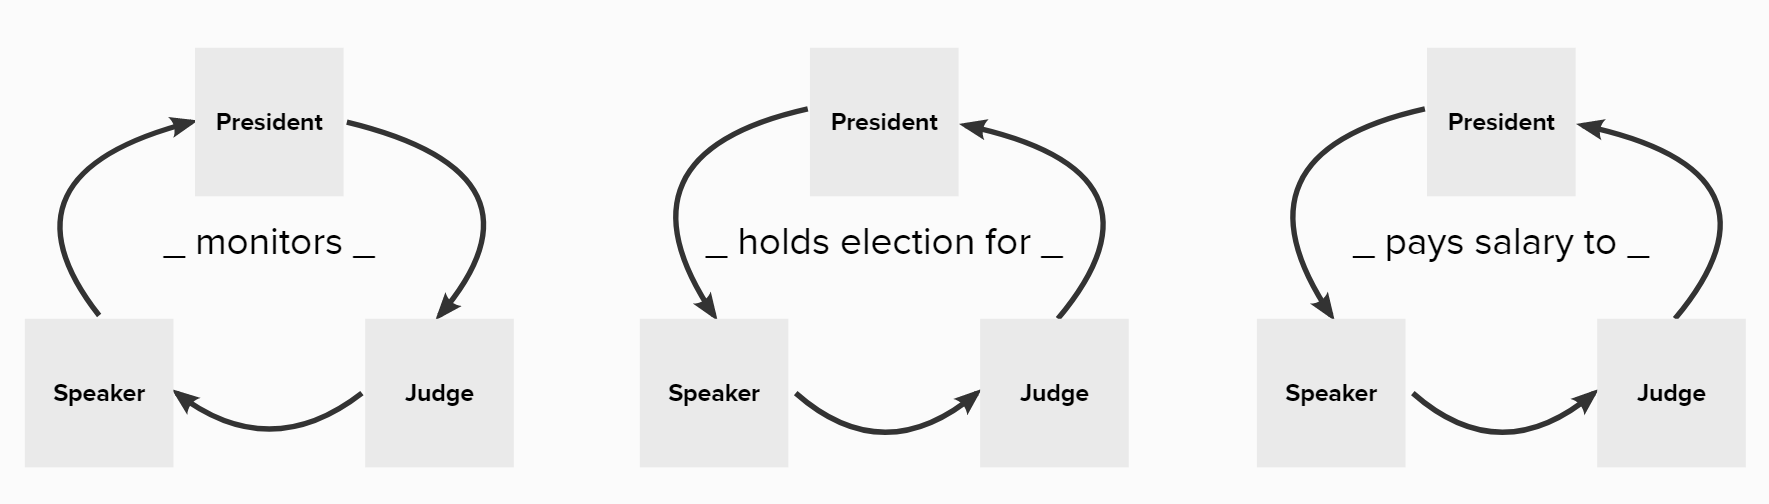
\includegraphics[scale=0.33]{05_iigo/images/role cycles.png}
\caption{Accountability cycle (left), the transfer-of-power cycle (middle) and salary cycle (right).}
\label{fig:cycles_in_IIGO}
\end{figure}


\subsection{Transfer-of-power}
\label{subsec:transfer-of-power}
\begin{enumerate}
    \item The Speaker conducts a vote for the election of the new Judge.
    \item The Judge conducts a vote for the election of the new President.
    \item The President conducts a vote for the election of the new Speaker.
\end{enumerate}
Refer to the Figure~ \ref{fig:cycles_in_IIGO} for further clarification about the transfer-of-power cycle.

\begin{rule_IIGO}
   The role $X$ has the \emph{obligation} to conduct a vote for the election of $Y$ at the end of the term (see Definition~\ref{def:term}) if and only if the role $X$ is accountable to the role $Y$. 
\end{rule_IIGO}.

\section{Budget and Salary}
\subsection{Budget}
%Actions associated with the IIGO have an associated cost that is defined as a configuration parameter. The institutional-power-enabled actions of  identified to require a "computational" component are:

Institutional-enabled-power actions in the IIGO have an associated cost with them. Some examples for such actions include:


%that is defined as a configuration parameter. The institutional-power-enabled actions of  identified to require a "computational" component are:


%We have defined the resource to be an endogenous one, hence any computation surrounding the distribution of the resource must use up some of that resource. 
\begin{itemize}
\item Calling any vote and computing the winner.
\item Declaring (e.g. \textit{announcing} the result of a vote).
\item Setting the amount of \emph{taxation} for each island.
\item Deciding the allocation distribution for each island.
\item Inspecting an island's action history.
\item Monitoring a role.
\end{itemize}

Since IIGO has been designed to act in the common good, IIGO-related costs will be directly withdrawn from the common pool. Since the common pool is considered a communal property of the archipelago, there are rules in place to limit how much each role is allowed to spend in order to perform its own institutional-power-enabled actions. This is the reason why defining the \emph{budget} and keeping it separate for each of the three IIGO roles.


As a role performs institutional-enabled-power actions, the corresponding cost associated with this action is subtracted from the role's budget. A budget of zero means that the role does not have the \emph{power} to perform any of its institutional-power-enabled actions. The removal of the budget rule from the rules in play means the role is allowed to perform as many such actions as it prefers to (as long as those actions are not governed by other rules). 



%As a role performs an endogenous-cost action, the corresponding cost associated with this action is subtracted from the role's budget. Thus, if as a result of an endogenous-cost action a role will be left with negative budget, it will have gone over the budget limit and will have broken the budget rule. A budget of zero means that the role is not allowed to perform any of its institutional-power-enabled actions associated an endogenous-cost. The removal of the budget rule from the rules in play means the role is allowed to perform as many such actions as it pleases (as long as those actions are not governed by other rules). 

The budget rule is also persistent across turns. This means that, assuming nothing else affects the budget, if a role has $100$ resources in its budget at each turn and spends only $10$ resources, this means that this very same role has $90$ resources in its budget at the next turn. On the other hand, islands can choose to increase the budget periodically every turn. This is governed by another budget extension rule.




%one turn and it spends 10, it has 90 resources in it's budget the next turn. 

Finally, it must be noted that the budget is inherently linked with the fact that whether obligations of a specific role can be undergone.
For example, during \emph{monitoring}, it should not be seen as a rule violation if a role has not acted on an obligation if it would go over the budget as a result. 

%This can also be seen as an added clause "... and the action is only permitted if they have the budget" to most rules which govern actions with an endogenous-cost.
%\begin{rule_IIGO}
    %The budget is increased by an amount $N$ every turn.
%\end{rule_IIGO}

%This rule means that, assuming nothing else affects the budget, if a budget is set to increase by 10 resources every turn and the budget is a 100 resources in turn one, the budget is 110 resources in turn 2. Setting this rule to 0 is equal to removing this rule and it means that the budget is never increased. 


\subsection{Salary}
\label{subsec:salary}
A salary is paid to each role in power as an incentive to act in a publicly approved way. %Hence, each role has the \emph{power} to pay a salary to another role following the salary cycle in Figure~\ref{fig:cycles_in_IIGO}.
\begin{rule_IIGO} \label{rule:salary}
   %Each role has the \emph{obligation} to pay the salary of amount $S$ to another if and only if the amount paid $S'$ is equal to $S$.
   Each role has the \emph{obligation} to pay the salary of amount $S$ to one another following the salary cycle in Figure~\ref{fig:cycles_in_IIGO}.
\end{rule_IIGO}

In Rule~\ref{rule:salary}, setting $S=0$ (through changing the active rules in place) means that roles do not have the permission to pay any salary. Removing the Rule~\ref{rule:salary} means that the roles may freely choose the amount $S$ for the salary payments.

\section{IIGO Session order}

\begin{enumerate}
    \item The Judge has the \emph{power} to check the history of actions to confirm whether the previously punished island(s) has/have obeyed the previous round's sanctions, meaning whether they contributed to the common pool accordingly in case of economic sanctions.
    %\begin{itemize}
      %  \item \emph{Suggested Rule:} In case of disobeying sanctions, the Judge is \emph{obliged} and \emph{permitted} to increase the severity of sanctions with respect to specific islands.
   % \end{itemize}
    \item The Judge has the \emph{power} to carry out \emph{inspections} on the history of actions of any island $X$ to check whether:
        \begin{enumerate}
        \item the reported resources of $X$ in the previous round match the real value of resources $X$ had in its private pool for the previous turn.
        \item the island $X$ has retrieved the right amount of the resources from the common pool, based on the \emph{allocation request} evaluated by the previous President.
            \begin{itemize}
            \item An example: In the previous round, the President has decided that the island $X$ can take $Y$ amount of resources from the common pool. If the Judge finds out that the island $X$ has taken an amount of $Y'$ such that $Y' > Y$, the Judge has the \emph{power} to invoke sanctions on the island $X$.
            
            %the Judge is \emph{obliged} and \emph{permitted} to sanction island $X$.
            \end{itemize}
        \end{enumerate}
    \item The Judge has the \emph{power} to invoke sanctions based on the outcome of the inspections.
    \item The President has the \emph{power} to decide to carry out a \emph{monitoring} on:
        \begin{enumerate}
        \item the sanctions imposed by the Judge.
        \end{enumerate}
    \item The islands may report the resources in their private pools to the President.
    \item The President has the \emph{power} to let each island know about the amount of \emph{taxation} they have to pay.
    \item The island has the \emph{power} to make an \emph{allocation request} to the President.
    \item The President has the \emph{power} decide on an allocation of resources and let each island know about the amount of resource allocation they are permitted to take from the common pool.
    \item The island has the \emph{power} to pick and to propose a rule to be voted on to the President.
    \item The President has the \emph{power} to choose a rule to be voted on from the received rule proposals.
    \item The Speaker has the \emph{power} to decide to carry out a \emph{monitoring} on: 
        \begin{enumerate}
        \item the resource allocation decided by the President.
        \item the rule proposed by the President.
        \end{enumerate}
    \item The Speaker has the \emph{power} to call a vote.
        \begin{enumerate}
        \item The islands vote in support of, or against, the rule (aye or nay) anonymously.
        \end{enumerate}
    \item The Speaker has the \emph{power} to announce a result of a vote to the islands and carries out the law change, if required (e.g. deleting/rejecting a rule if there is a majority nay vote).
    \item The Judge has the \emph{power} to decide to carry out \emph{monitoring} on:
        \begin{enumerate}
        \item the vote called by the Speaker.
        \item the Speaker announcing the result.
    \end{enumerate}
    \item The roles pay salary for one another following the accountability cycle in Figure~ \ref{fig:cycles_in_IIGO}.

\end{enumerate}



\section{Future Work}

\begin{itemize}
    \item \textbf{Diplomatic sanctions}: Although having the potential of being a good alternative for severer sanctions discussed in  Section~\ref{sec:sanctions}, diplomatic sanctions are \emph{not} implemented within the scope of the coursework. \\
    Suggested diplomatic sanctions include:
        \begin{itemize}
            \item Revoking an island's eligibility to vote and to be elected for a position.
            \item Revoking an island's eligibility to propose a rule/motion.
        \end{itemize}
    \item \textbf{Immutable rules}: Within the scope of the coursework, a subset of rules could have been categorised as immutable. This means that to change such immutable rules, the islands first need to vote to change their status to be \emph{mutable}, and consequently, hold another vote to change these mutable rules.
    %\item \textbf{Adding rules to the proposal list: } 
\end{itemize}

    \chapter{Inter-Island Governmental Organisation (IIGO)}


The role of IIGO is to maintain, update, and revise the rules concerning provision to managing the long-term collective risk dilemma (ltCRD). 

\begin{itemize}
    \item There will be 3 distinct branches in the IIGO: the \textbf{legislative branch}, \textbf{executive branch} and \textbf{judicial branch}\footnote{This is, as no surprise, inspired by the separation of powers in Western democracies.}.
    \item Each role is put in power according to the  transfer-of-power rules (see Section~\ref{subsec:transfer-of-power} for more detail).
    \item The head of the legislative branch is the Speaker, the head of the executive branch is the President, and the head of judicial branch is the Judge.
    \begin{itemize}
        \item  The Speaker, President and Judge are selected, through a democratic election, from the islands in the archipelago\footnote{This naming is inspired by the roles in the US Government.}.
        \item The resources gathered by the archipelago are endogenous, hence acting on the institutional powers granted to the Speaker, President or Judge costs resources. 
        \item For their duty, the President, the Speaker and the Judge receive a salary for each of their turns in office (see Section~\ref{subsec:salary} for more detail).
        \item The limit of the powers of the President, Speaker and Judge are defined in this chapter (e.g. the Speaker can only call one vote per turn).
 
    \end{itemize}
\end{itemize}

\subsection{IIGO Specific Definitions}
\begin{definition} \label{def:ballot}
    A \textbf{ballot} is related to each island's \textbf{power} to support or disagree with the rule specified in the vote called by the President and to vote in favour or against an island for a specific role (i.e. the President, Speaker, Judge) at each round of the game.
\end{definition}


%\begin{definition} \label{def:vote}
    %A \textbf{vote} is related to a role's (i.e. the President, Speaker, Judge) \textbf{power} to call a vote for a specific rule or an election.
%\end{definition}


\begin{definition} \label{def:tax}
    The \textbf{taxation} is related to the President's \textbf{power} to request a specific \underline{\textbf{minimum}} amount of contribution from each island to the common pool at each round of the game. 
\end{definition}

\begin{definition} \label{def:alloc_req}
    An \textbf{allocation request} is related to each island's \textbf{power} to request a specific amount of resource allocation from the President at each round of the game.
\end{definition}


\begin{definition} \label{def:rule_prop_list}
A \textbf{rule proposal list} is related to each island's \textbf{power} to propose a specific rule to be passed to the President at each round of the game.
\end{definition}

\begin{definition} \label{def:invst}
    An \textbf{investigation} is related to the Judge's \textbf{power} to acquire information to make a decision, followed by a calculation of the expected results and checking whether some specific rules have been obeyed, exclusively for the actions carried out by the \textbf{islands}. 
\end{definition}


An example of an \emph{investigation}: The President has permitted the island $X$ to take the amount of $Y$ resources from the common pool. Upon \emph{investigation} carried out by the Judge, it is revealed that the amount of resources taken out from the common pool by the island $X$ is, in fact, $Y'$ such that $Y' \neq Y$.


\begin{definition}
\textbf{Monitoring} is a government official's \textbf{power} to perform event recognition and to check whether some specific rules have been obeyed.
\end{definition}

An example of \emph{monitoring}: The Speaker has performed only the following action: \emph{counted the votes and calculated the result} for a rule. Upon \emph{monitoring} carried out by the President, it is noticed that the Speaker has not made any \emph{announcement}. Hence, the Speaker has not followed their obligation to \emph{announce} the result of any vote held.

See Section~\ref{sec:accountability} for more information about which roles can monitor which ones.


\begin{definition}
\textbf{Investigative-monitoring} is a government official's \textbf{power} to acquire the information used in acting on a governmental power followed by calculation of the expected results and checking whether some specific rules have been obeyed, exclusively for the actions carried out by a government official they are responsible for.
\end{definition}

An example of \emph{investigative-monitoring}: The Speaker has performed the following actions: \emph{counted the votes and calculated the result $R$} for a vote $V$ and \emph{announced} the result $R'$ for the vote $V$. Upon \emph{investigative-monitoring} carried out by the President, it is noticed that $R' \neq R$. Hence, the Speaker has modified the announced result.


\begin{definition}
The \textbf{sanction} is related to the Judge's \emph{power} to punish non-compliant islands when their disobedience is confirmed through investigations at a specific turn.
\end{definition}


\begin{definition}
The (judicial) \textbf{pardon} is related to the Judge's \emph{power} to forgive a non-compliant island at a specific turn.
\end{definition}

\begin{definition}
The \textbf{budget} is the maximum amount of resources a role is permitted to spend from the common pool as it performs its own institutional-power-enabled actions at a specific turn.
\end{definition}


\begin{definition}
The \textbf{salary} is the amount of resources a role is to be given from the common pool as a reward for performing its institutional-power-enabled actions at a specific turn.
\end{definition}

\begin{definition} \label{def:term}
A \textbf{term} is the number of turns an island is \emph{permitted} to hold a role, and after which the responsible role (indicated in the transfer-of-power cycle in Figure~\ref{fig:cycles_in_IIGO}) is \emph{obliged} to initiate transfer-of-power.
\end{definition}

\subsection{\emph{Power}, \emph{Permission} and \emph{Obligation} Distinction}
In the rest of the specifications, we will be specifically using the following three terms to define the actions and responsibilities carried out by the Speaker, President, Judge (see Figure~ \ref{fig:per_obl_sets}):
\begin{itemize}
    \item Power
    \item Permission
    \item Obligation
\end{itemize}



\begin{figure}[H] 
\centering
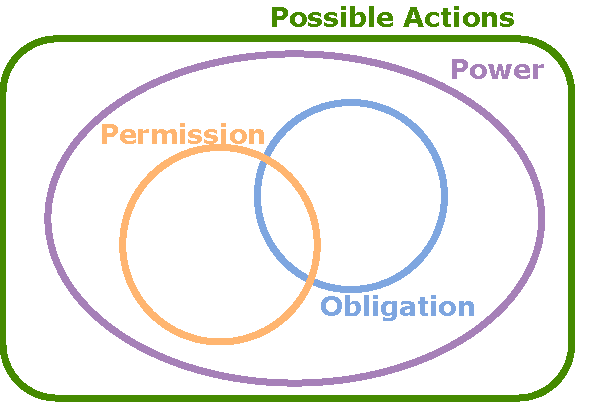
\includegraphics[width=0.6\textwidth]{05_iigo/images/SOMAS_per_obl.pdf}
\caption{Relationship between \emph{power}, \emph{permission} and \emph{obligation}.}
\label{fig:per_obl_sets}
\end{figure} 


For example, the Judge has the \emph{power} to carry out investigations at an IIGO session. There are no rules specifying which specific islands the Judge should investigate. Therefore, the Judge has the \emph{permission} to investigate any `alive' islands during a session. However, the Judge is \emph{obliged} to make at least some number of investigations each turn.



\section{Executive Branch}
\label{sec:executive}
The executive branch is responsible for \textbf{carrying out the law}.
\begin{itemize}
       
    \item The President has the \emph{power} to: 
    \begin{itemize}
        
        \item Select a rule for voting $R^{*}$ to be passed to the Speaker.
        \begin{rule_IIGO}
            The President has the \emph{obligation} to \emph{select} a rule $R^{*}$ if the \emph{rule proposal list} has at least one proposed rule in it.
        \end{rule_IIGO}
        \begin{rule_IIGO}
            The President has the \emph{permission} to \emph{select} a rule $R^{*}$ if and only if $R^{*} \in S$, where $S$ is the \emph{rule proposal list}.
        \end{rule_IIGO}
        
        \item Decide the amount of individual \emph{taxation} (i.e. a specific \emph{minimum} amount of contribution to the common pool for each island) for the current turn.
        
        \begin{itemize}
            \item The President is given the self-reported resource amounts held by each island to assist in this decision.
            %\item Suggested Rule: For any island that has chosen to not report it's resources, the President has the \emph{obligation} to set them an individual tax amount T.
        \end{itemize}
        
        \item Decide the allocation of resources distributed from the common pool to the islands (i.e. a specific \emph{maximum} amount an island is permitted to take from the common pool).
        
        \begin{itemize}
            \item The President is given the \emph{allocation requests} made by each island.
            %\item \emph{}{Suggested Rule:} The President has an obligation to prioritise islands in critical condition.
        \end{itemize}
    \end{itemize}
\end{itemize}



\section{Legislative Branch}
\label{sec:legislative}
The legislative branch is responsible for \textbf{making the law}.
\begin{itemize}

    \item The Speaker has the \emph{power} to:
    \begin{itemize}
        
        \item Call a vote $V$ for a rule $R$.
        \begin{rule_IIGO}
            The Speaker has the \emph{obligation} to \emph{call} a vote $V$ if and only if the President has \emph{selected} a rule $R$ to be voted on.
        \end {rule_IIGO}
        \begin{rule_IIGO}
            The Speaker has the \emph{permission} to \emph{call} a vote $V$ for a rule $R$ if and only if the rule $R = R^{*}$, where $R^{*}$ is the rule \emph{selected} by the President.
        \end {rule_IIGO}
            
        \item Choose which islands are participating in the vote $V$.
       % \footnote{This is our sequential implementation alternative for the power to close the ballot box.}.
        \begin{rule_IIGO}
            The Speaker has the \emph{obligation} to ask for a vote from all alive islands.
        \end {rule_IIGO}
            
        \item Declare the result $C$ of a vote $V$. 
        \begin{rule_IIGO}
            The Speaker has the \emph{obligation} to \emph{declare the result} $C$ for a vote $V$ if and only if the vote V has been \emph{called}.
        \end {rule_IIGO}
        \begin{rule_IIGO}
            The Speaker has the \emph{permission} to \emph{declare the result} $C$ for a vote $V$ if $C = C^{*}$, where $C^{*}$ is the result produced by \emph{calling} the vote $V$.
        \end {rule_IIGO}
        \begin{itemize}
            \item This step is what enables a rule to be \emph{active}.
        \end{itemize}
    \end{itemize}
\end{itemize}




\section{Judicial Branch}
\label{sec:judicial}

The judicial branch is responsible for \textbf{evaluating the law}.
\begin{itemize}
    \item The Judge has the \emph{power} to:
    \begin{itemize}
        \item Perform a number of \emph{inspections}\footnote{An \emph{inspection} \textbf{costs} an expense of resources (See Definition~\ref{def:invst} for more detail).} $I$ and produce a compliance outcome $\mathbb{O}^{*}$\footnote{Note that the compliance outcome $\mathbb{O}^{*}$ considered is a boolean.}.
        %(true: the island has been compliant with the rules in play, false: the island has not been compliant with the rules in play)
        %\begin{itemize}
           % \item For example, to check if the event outcome is \emph{concurrent}\footnote{Again, what is defined as "concurrent"? A clear definition is needed.} with the rules.
        %\end{itemize}
        \begin{rule_IIGO}
            The Judge has the \emph{obligation} to make at least $N$ investigations at each turn.
        \end{rule_IIGO}
        \item Declare the outcome $\mathbb{O}$ of an inspection $I$ to all islands\footnote{This act of broadcasting is especially important for islands to form an opinion about the sanctioned islands accordingly.}.
        \begin{rule_IIGO}
            The Judge has the \emph{obligation} to declare the outcome $\mathbb{O}$ of an inspection $I$ if and only if the inspection $I$ has been performed.
        \end{rule_IIGO}
        \begin{rule_IIGO}
            The Judge has the \emph{permission} to declare the outcome $\mathbb{O}$ of an inspection $I$ if $\mathbb{O} = \mathbb{O}^{*}$, where $\mathbb{O}^{*}$ is the outcome of the inspection $I$.
        \end{rule_IIGO}
        %\item Initiate the removal of the \texttt{President}.
        %\begin{itemize}
            %\item A good Judge would be especially vigilant during \emph{power transfer} regarding the \emph{President} position (see Section~\ref{leg_const} for more detail).
        %\end{itemize}
        \item Invoke economic \textbf{sanctions} (see Section~\ref{sec:sanctions} for more detail).
        \begin{rule_IIGO}
            The Judge has the \emph{obligation} to invoke a sanction $S$ for an island $X$ if and only if an investigation $I$ has an outcome $\mathbb{O}^{*}$ indicating non-compliance, and $I$ is an investigation of an action taken by island $X$.
        \end{rule_IIGO}
        \item Invoke even more severe sanctions in the case of further disobedience to previous sanction(s).
        \begin{rule_IIGO}
            The Judge has the \emph{permission} to invoke a severer sanction $S'$ for an island $X$ if the island $X$ has not fulfilled the requirements of the previous sanction $S$.
        \end{rule_IIGO}
        \item Pardon the islands which are currently sanctioned.
        \begin{rule_IIGO}
            The Judge has the \emph{permission} to revoke any sanction $S$ of an island $X$ at a specific turn.
        \end{rule_IIGO}
    \end{itemize}
\end{itemize}
%(e.g. a new rule that falls under a "sanction" category \hl{[I'm not sure about this being a `new rule` [Ezgi]]}

\subsection{Sanctions}
\label{sec:sanctions}
All sanctions are of economic nature which include:
        \begin{itemize}
            %\item Revoking an island's access to the common pool.
            \item Enforcing an island to contribute a specific amount of resources to the common pool.
            \begin{itemize}
                \item This does not mean that the Judge has the \emph{power} to take resources from an island in order to put them to the common pool -- the island itself is expected to carry out this implication imposed by the sanction itself, otherwise further punishment can be induced by the Judge.
                \item Similarly, \emph{opinion formulation} will follow accordingly whether the island(s) is/are following the implications imposed by the sanction(s).
            \end{itemize}
        
    \end{itemize}
    Sanctions are the associated penalty that comes with an island breaking a specific rule. The Judge is in full control of the penalties associated with breaking any rules. Once the Judge has specified the score of the penalty associated with each time an island breaks a rule, the cumulative penalties accumulated by the island are then used to determine which \textbf{sanction tier} that each island falls into. The score threshold to determine the boundaries of the sanction tiers are set by the Judge. At each turn of the game, each island is told whether they are being sanctioned, and if so, which \textbf{sanction tier} that they are currently in. The \textbf{sanction tiers} of the non-compliant islands are also broadcasted to the other islands in the archipelago. To summarise, the sanctioning process follows these steps:
    
    
    
    %Sanctions are based on an island breaking a rule. Each rule must therefore have an associated penalty. By default, we set these penalties such that they add $1$ to the total sanction score for each island. However, we allow the judge to override this scoring, the judge is able to set their own scores for any particular rule as they desire. This custom scoring is then used when an island breaks a particular rule. By looking at events that occurred in the last turn, and using the customised scoring we provide the holder of the judge role with full control of the penalties for breaking any rules.
    
    





%we then use the cumulative penalties accumulated by each island to determine which Sanction Tier they fall into. The score threshold's required to fall into these sanction tiers is set by the judge and is checked for monotonicity. Each island is told whether they are being sanctioned, and is so what tier they are in. We also tell other islands about which sanction tiers other islands have fallen into. 

    \begin{enumerate}
        \item The Judge has the \emph{power} to set custom penalties associated with breaking any rules.
        \item The Judge is given a list of all events that occurred in the previous turn.
        \item The Judge has the \emph{power} to check whether any, or all of these previous events, involve the islands in the archipelago breaking any rules.
        \item Each of the transgressions is scored using the Judge's custom penalties if the Judge has set them. Otherwise, a score of $1$ is given each time a rule is broken.
        \item The Judge has the \emph{power} to revise the sanction thresholds.
        \item Using the latest sanction thresholds available, each island is assigned to a sanction tier based on the sanction score that it has received.
        \item These sanction tiers are broadcasted to all of the islands in the archipelago.
        \item The Judge then uses sanctions rules in place to calculate the specific amount of resources that each non-compliant island has in order to determine how much it should contribute to the common pool, based on the sanction tier that it is in.
    \end{enumerate}



\section{Constitutional Rights and Obligations in the Archipelago}
\label{sec:const_rights_obl_archi}
Each island has the \emph{power} to:
\begin{itemize}
\item make an \emph{allocation request} (see Definition~\ref{def:alloc_req}) to the President for a specific amount to be allocated to them.
\item report the number of resources it is in possession of to the President.
\begin{rule_IIGO}
    Each island has the \emph{obligation} to report the number of resources it is in possession of to the President.
\end{rule_IIGO}
\begin{rule_IIGO}
    Each island has the \emph{permission} to report the number of resources $R'$ if and only if $R' = R$, where R is the number of resources the island is in possession of.
\end{rule_IIGO}
\item take resources from the common pool.


\begin{rule_IIGO}
    Each island has the \emph{permission} to take at maximum $N$ resources, where $N$ is the specific allocation made by the President to that island\footnote{If no such allocation is made, the island is \emph{permitted} to take any amount of resources.}.
\end{rule_IIGO}
\item contribute resources to the common pool.
\begin{rule_IIGO}
    Each island has the \emph{obligation} to contribute to the common pool an amount greater or equal to that of the individual tax set by the President.
\end{rule_IIGO}
                %The President is in
                %(unless there is a rule in place that dictates how Speaker is to allocate resources).
\item add a rule to the \emph{rule proposal list} (see Definition~\ref{def:rule_prop_list}) at the start of each turn.
        %\begin{itemize}
            %\item The game specification includes how many rules an island can propose each turn.
        %\end{itemize}
        %\item vote  for rules in the Legislative Branch and vote for their favourite islands in elections
\item participate in the legislative branch of the government by casting ballots in votes called by the Speaker
\item vote for an island to be elected for a specific role (e.g. the President, Judge, Speaker) during the elections\footnote{This will be assumed to be true \underline{unless stated otherwise}. %Note that \textbf{diplomatic sanctions} can disable this power of a specific island (see Section~\ref{jud_const}).}.
        }.
\end{itemize}
\section{Accountability Cycle}
\label{sec:accountability}


To ensure that the government avoids corruption and abuse of power, each branch is accountable to another. The President is accountable to the Speaker, the Speaker is accountable to the Judge, and the Judge is accountable to the President (see Figure~ \ref{fig:cycles_in_IIGO}). This accountability cycle is enacted through \emph{monitoring} actions\footnote{Note that the terms \textbf{monitoring} and \textbf{investigation} have similar but quite different meanings in the IIGO context.}. 

The powers related to the accountability cycle and transfer-of-power for each role can be summarized as the following: 
\begin{itemize}
    \item The Speaker has the \emph{power} to: 
    \begin{itemize}
        \item monitor the President.
        \item announce the result of this monitoring.
        \item initiate the transfer-of-power for the Judge.
    \end{itemize}
    \item The President has the \emph{power} to: 
    \begin{itemize}
        \item monitor the Judge.
        \item announce the result of this monitoring.
        \item initiate the transfer-of-power for the Speaker.
    \end{itemize}
    \item The Judge has the \emph{power} to: 
    \begin{itemize}
        \item  monitor the Speaker.
        \item announce the result of this monitoring.
        \item initiate the transfer-of-power for the President.
    \end{itemize}
\end{itemize}

%Unlike investigations performed by the Judge, who performs investigations on island actions in the following turn, each role is given the opportunity to check up on the actions of the role it is responsible for immediately after they have been performed. In this sense, the President can monitor (includes investigative-monitoring) the powers (calling a vote and announcing the result) acted on by the Speaker immediately after the Speaker's announcement (or lack there of). The government officials hold a lot of power so this is to ensure that any wrong-doing is determined as quickly as possible. For this project we are only pursuing one degree of monitoring, that is, the powers relating to the accountability cycle will not be monitored themselves. We assume that agents will act in the interest of themselves and keeping all the islands alive is beneficial to everyone. Hence, while the agents might be inclined to break rules in order to benefit themselves, anyone else breaking the rules is seen as undesirable under the assumption that the system in place is there to benefit all. 


Through the proposed accountability cycle, each role is given the opportunity to check up on the actions of the role it is accountable for immediately after they have been performed. It is clear that the IIGO roles (i.e. the President, Speaker and Judge) hold a considerable amount of \emph{power} in their hands. The accountability cycle is designed to address the possible abuses of this power. With monitoring, any wrong-doing in the IGO is determined as quickly as possible and the role in question can be replaced. 

Within the scope of the coursework, we decided to pursue only \emph{one degree of monitoring}, meaning that the powers relating to the accountability cycle will not be monitored themselves. We assume that agents will act in the interest of all the islands in the archipelago. Hence, while the agents might be inclined to break the rules to benefit in some form, it is assumed that the others will negatively see any non-compliant islands based on the assumption that the proposed IIGO system is in place to maintain the welfare of all the islands.

Let role $X$ be accountable to the role $Y$, which is accountable to the role $Z$. Then:
\begin{rule_IIGO}
$Y$ has the \emph{obligation} to declare the outcome of the monitoring result $M$ associated with the action $A$ undertaken by $X$ if and only if $Y$ has monitored the action $A$ performed by $X$. 
\end{rule_IIGO}
\begin{rule_IIGO}
$Y$ has the \emph{permission} to declare the monitoring result $M$ associated with the action $A$ undertaken by $X$ if and only if $M = M^{*}$, where $M^{*}$ is the outcome of \emph{monitoring} action $A$ performed by $X$\footnote{These constitutional rules should be available to the agents to check their decision against. However, due to having only one degree of accountability cycle in place, these rules are not enforced through any sanctions (i.e. breaking these rules has no consequences as they only deem to be an \emph{agreement} among the roles).}.
\end{rule_IIGO}


\begin{figure}[!htb]
\centering
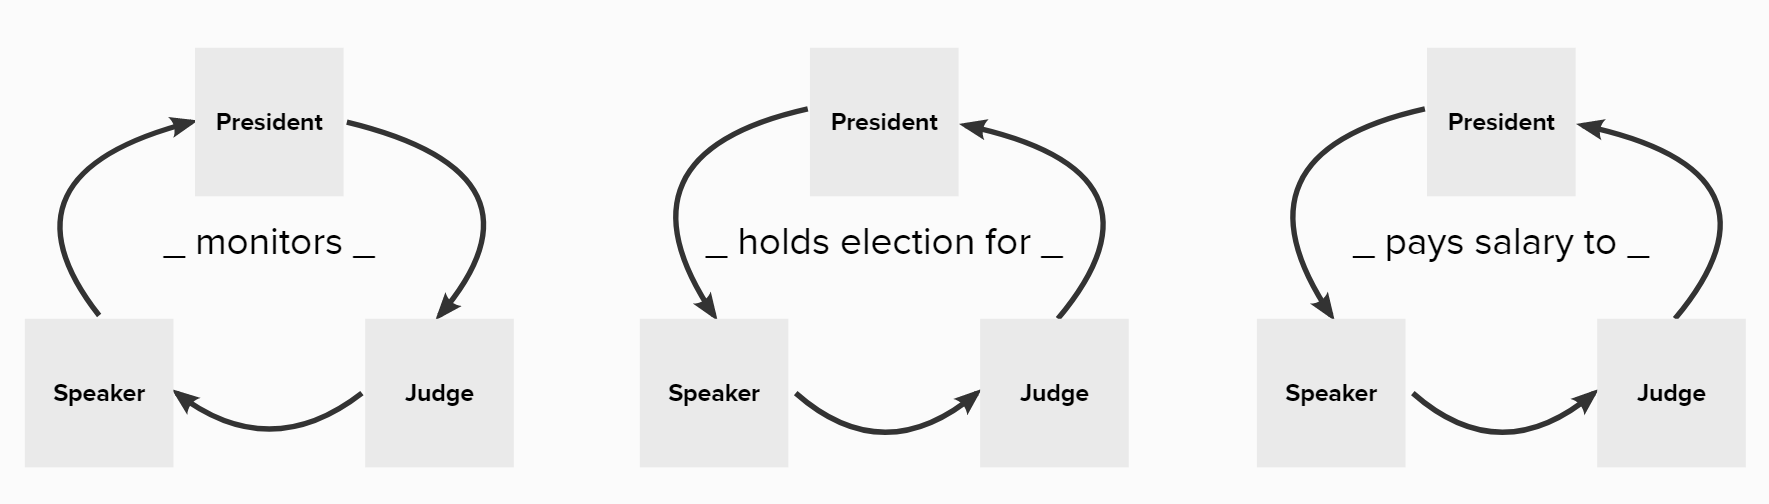
\includegraphics[scale=0.33]{05_iigo/images/role cycles.png}
\caption{Accountability cycle (left), the transfer-of-power cycle (middle) and salary cycle (right).}
\label{fig:cycles_in_IIGO}
\end{figure}


\subsection{Transfer-of-power}
\label{subsec:transfer-of-power}
\begin{enumerate}
    \item The Speaker conducts a vote for the election of the new Judge.
    \item The Judge conducts a vote for the election of the new President.
    \item The President conducts a vote for the election of the new Speaker.
\end{enumerate}
Refer to the Figure~ \ref{fig:cycles_in_IIGO} for further clarification about the transfer-of-power cycle.

\begin{rule_IIGO}
   The role $X$ has the \emph{obligation} to conduct a vote for the election of $Y$ at the end of the term (see Definition~\ref{def:term}) if and only if the role $X$ is accountable to the role $Y$. 
\end{rule_IIGO}.

\section{Budget and Salary}
\subsection{Budget}
%Actions associated with the IIGO have an associated cost that is defined as a configuration parameter. The institutional-power-enabled actions of  identified to require a "computational" component are:

Institutional-enabled-power actions in the IIGO have an associated cost with them. Some examples for such actions include:


%that is defined as a configuration parameter. The institutional-power-enabled actions of  identified to require a "computational" component are:


%We have defined the resource to be an endogenous one, hence any computation surrounding the distribution of the resource must use up some of that resource. 
\begin{itemize}
\item Calling any vote and computing the winner.
\item Declaring (e.g. \textit{announcing} the result of a vote).
\item Setting the amount of \emph{taxation} for each island.
\item Deciding the allocation distribution for each island.
\item Inspecting an island's action history.
\item Monitoring a role.
\end{itemize}

Since IIGO has been designed to act in the common good, IIGO-related costs will be directly withdrawn from the common pool. Since the common pool is considered a communal property of the archipelago, there are rules in place to limit how much each role is allowed to spend in order to perform its own institutional-power-enabled actions. This is the reason why defining the \emph{budget} and keeping it separate for each of the three IIGO roles.


As a role performs institutional-enabled-power actions, the corresponding cost associated with this action is subtracted from the role's budget. A budget of zero means that the role does not have the \emph{power} to perform any of its institutional-power-enabled actions. The removal of the budget rule from the rules in play means the role is allowed to perform as many such actions as it prefers to (as long as those actions are not governed by other rules). 



%As a role performs an endogenous-cost action, the corresponding cost associated with this action is subtracted from the role's budget. Thus, if as a result of an endogenous-cost action a role will be left with negative budget, it will have gone over the budget limit and will have broken the budget rule. A budget of zero means that the role is not allowed to perform any of its institutional-power-enabled actions associated an endogenous-cost. The removal of the budget rule from the rules in play means the role is allowed to perform as many such actions as it pleases (as long as those actions are not governed by other rules). 

The budget rule is also persistent across turns. This means that, assuming nothing else affects the budget, if a role has $100$ resources in its budget at each turn and spends only $10$ resources, this means that this very same role has $90$ resources in its budget at the next turn. On the other hand, islands can choose to increase the budget periodically every turn. This is governed by another budget extension rule.




%one turn and it spends 10, it has 90 resources in it's budget the next turn. 

Finally, it must be noted that the budget is inherently linked with the fact that whether obligations of a specific role can be undergone.
For example, during \emph{monitoring}, it should not be seen as a rule violation if a role has not acted on an obligation if it would go over the budget as a result. 

%This can also be seen as an added clause "... and the action is only permitted if they have the budget" to most rules which govern actions with an endogenous-cost.
%\begin{rule_IIGO}
    %The budget is increased by an amount $N$ every turn.
%\end{rule_IIGO}

%This rule means that, assuming nothing else affects the budget, if a budget is set to increase by 10 resources every turn and the budget is a 100 resources in turn one, the budget is 110 resources in turn 2. Setting this rule to 0 is equal to removing this rule and it means that the budget is never increased. 


\subsection{Salary}
\label{subsec:salary}
A salary is paid to each role in power as an incentive to act in a publicly approved way. %Hence, each role has the \emph{power} to pay a salary to another role following the salary cycle in Figure~\ref{fig:cycles_in_IIGO}.
\begin{rule_IIGO} \label{rule:salary}
   %Each role has the \emph{obligation} to pay the salary of amount $S$ to another if and only if the amount paid $S'$ is equal to $S$.
   Each role has the \emph{obligation} to pay the salary of amount $S$ to one another following the salary cycle in Figure~\ref{fig:cycles_in_IIGO}.
\end{rule_IIGO}

In Rule~\ref{rule:salary}, setting $S=0$ (through changing the active rules in place) means that roles do not have the permission to pay any salary. Removing the Rule~\ref{rule:salary} means that the roles may freely choose the amount $S$ for the salary payments.

\section{IIGO Session order}

\begin{enumerate}
    \item The Judge has the \emph{power} to check the history of actions to confirm whether the previously punished island(s) has/have obeyed the previous round's sanctions, meaning whether they contributed to the common pool accordingly in case of economic sanctions.
    %\begin{itemize}
      %  \item \emph{Suggested Rule:} In case of disobeying sanctions, the Judge is \emph{obliged} and \emph{permitted} to increase the severity of sanctions with respect to specific islands.
   % \end{itemize}
    \item The Judge has the \emph{power} to carry out \emph{inspections} on the history of actions of any island $X$ to check whether:
        \begin{enumerate}
        \item the reported resources of $X$ in the previous round match the real value of resources $X$ had in its private pool for the previous turn.
        \item the island $X$ has retrieved the right amount of the resources from the common pool, based on the \emph{allocation request} evaluated by the previous President.
            \begin{itemize}
            \item An example: In the previous round, the President has decided that the island $X$ can take $Y$ amount of resources from the common pool. If the Judge finds out that the island $X$ has taken an amount of $Y'$ such that $Y' > Y$, the Judge has the \emph{power} to invoke sanctions on the island $X$.
            
            %the Judge is \emph{obliged} and \emph{permitted} to sanction island $X$.
            \end{itemize}
        \end{enumerate}
    \item The Judge has the \emph{power} to invoke sanctions based on the outcome of the inspections.
    \item The President has the \emph{power} to decide to carry out a \emph{monitoring} on:
        \begin{enumerate}
        \item the sanctions imposed by the Judge.
        \end{enumerate}
    \item The islands may report the resources in their private pools to the President.
    \item The President has the \emph{power} to let each island know about the amount of \emph{taxation} they have to pay.
    \item The island has the \emph{power} to make an \emph{allocation request} to the President.
    \item The President has the \emph{power} decide on an allocation of resources and let each island know about the amount of resource allocation they are permitted to take from the common pool.
    \item The island has the \emph{power} to pick and to propose a rule to be voted on to the President.
    \item The President has the \emph{power} to choose a rule to be voted on from the received rule proposals.
    \item The Speaker has the \emph{power} to decide to carry out a \emph{monitoring} on: 
        \begin{enumerate}
        \item the resource allocation decided by the President.
        \item the rule proposed by the President.
        \end{enumerate}
    \item The Speaker has the \emph{power} to call a vote.
        \begin{enumerate}
        \item The islands vote in support of, or against, the rule (aye or nay) anonymously.
        \end{enumerate}
    \item The Speaker has the \emph{power} to announce a result of a vote to the islands and carries out the law change, if required (e.g. deleting/rejecting a rule if there is a majority nay vote).
    \item The Judge has the \emph{power} to decide to carry out \emph{monitoring} on:
        \begin{enumerate}
        \item the vote called by the Speaker.
        \item the Speaker announcing the result.
    \end{enumerate}
    \item The roles pay salary for one another following the accountability cycle in Figure~ \ref{fig:cycles_in_IIGO}.

\end{enumerate}



\section{Future Work}

\begin{itemize}
    \item \textbf{Diplomatic sanctions}: Although having the potential of being a good alternative for severer sanctions discussed in  Section~\ref{sec:sanctions}, diplomatic sanctions are \emph{not} implemented within the scope of the coursework. \\
    Suggested diplomatic sanctions include:
        \begin{itemize}
            \item Revoking an island's eligibility to vote and to be elected for a position.
            \item Revoking an island's eligibility to propose a rule/motion.
        \end{itemize}
    \item \textbf{Immutable rules}: Within the scope of the coursework, a subset of rules could have been categorised as immutable. This means that to change such immutable rules, the islands first need to vote to change their status to be \emph{mutable}, and consequently, hold another vote to change these mutable rules.
    %\item \textbf{Adding rules to the proposal list: } 
\end{itemize}

    \chapter{Game Design}

\section{Implementation}
\label{sec:GD:implementation}

Implementation design was important as the majority of the class were involved in writing simulation code. As such, dedicated \emph{infrastructure} engineers from each team were elected to form an infrastructure team responsible for building the central part of the game, otherwise known as the \emph{server}. Each team's infrastructure engineer was tasked to own the implementation of a slice of the server.

One such sub-team was the \textbf{core} infrastructure team, responsible for building the core parts of the game server. Inputs were taken from the entire class to choose the best implementation strategies and design--a solid and simple core foundation was paramount to allow clean continuous integration of code and ideas from all contributors. The subsections below detail implementation specifics of the game's simulation.

\subsection{Architecture}
\label{sec:GD:implementation:arch}

The structure of the game was closely modelled after a \emph{client-server} model\footnote{\url{https://en.wikipedia.org/wiki/Client-server_model}}, but note ``closely''--whilst the nomenclature was taken directly from the aforementioned model, there are some differences. \emph{Server} and \emph{client} in this context bear the following definitions:

\begin{definition} \label{def:server}
    The \textbf{server} is the central game runner, responsible for initiating game events (such as a disaster or the start of a turn). Certain events require the actions of agents, in which the server will invoke a function on the agents to receive a response. Further, the server acts as a source-of-truth for the game's state.
\end{definition}


\begin{definition} \label{def:client}
    Each \textbf{client} is implemented by an agent. The client provides an interface of functions in which the server can invoke. Moreover, clients may also invoke certain functions from the server's interface to read specific game information.
\end{definition}

The major difference of this architecture to a traditional client-server model is that, in the former, the stateful central server drives the other clients (by triggering events and eliciting responses), as opposed to clients sending stateless requests to a server to receive a response in the latter. Furthermore, whilst the client and server have been separated architecturally, the entire system still operates as a single process.

\subsection{Technology Stack}
\label{sec:GD:implementation:techstack}

Agreeing on a technology stack proved to be challenging--the class had varying levels of programming expertise. Whilst Prolog\footnote{\url{https://en.wikipedia.org/wiki/Prolog}} and Qu-Prolog\footnote{\url{https://staff.itee.uq.edu.au/pjr/HomePages/QuPrologHome.html}} (an extension to the former) were used to cover topics in the lectures, the class did not favour them over more well-known and established imperative programming languages. Hence, time was dedicated to formulate a consensus to decide on the technology stack, with primary focus given on the choice of implementation language. Firstly, high priority requirements were defined for the stack:

\begin{itemize}
    \item Easy to learn
    \item Easy to setup
    \item Cross-platform
    \item Easily maintainable
    \item Friendly features
\end{itemize}

Minimum Working Examples (MWEs) comprising a single server and two clients were created in different stacks, which served as starting points for discussion among members of the class. The MWEs implemented are as follows.

\begin{enumerate}
    \item \textbf{Multi-language}\footnote{\url{https://github.com/SOMAS2020/somas-demo}}.
          A multi-language (C++ server with a Python and a C++ client) MWE was first set up. It was first thought that allowing agent teams to choose the programming language they were most familiar with would speed up development. However, despite this stack's benefits, it could not be easily made cross-platform. Each agent's code would need to be run in a separate process, and Inter-Process Communication (IPC) would be required to pass messages. IPC is quite low-level and varies vastly among different systems. Further, protocols for the IPC would also need to be set up to pass the correct message, and having no strong typing as in a strongly-typed language (or session-typed\footnote{\url{https://arxiv.org/abs/1906.03836}}) approach would make it difficult to maintain and develop.

    \item \textbf{Python}\footnote{\url{https://github.com/SOMAS2020/somas-demo-py}}.
          Python\footnote{\url{https://www.python.org/}} is widely used by the scientific community in recent years with the growing ubiquity of scientific computation packages available for it. As such, Python was a strong contender as most of the class already know Python from past projects. However, Python's weak typing meant it scored low on the ``easily maintainable'' part--the server and client interfaces would benefit a lot from strong typing. While add-on static typing tools such as \texttt{mypy}\footnote{\url{https://mypy.readthedocs.io/}} could be employed (it is also used in the MWE), it would still not be as powerful as built-in strong typing as in languages such as C\# and Go.

    \item \textbf{C\#}\footnote{\url{https://github.com/SOMAS2020/somas-demo-cs}}.
          C\#\footnote{\url{https://docs.microsoft.com/en-us/dotnet/csharp/}} is the flagship language of the .NET ecosystem. C\# shares a large part of its design to the more popular C++. C\# is strongly-typed, and promotes use of clean Object-Oriented Programming (OOP). Many of the features from C/C++ that can be \emph{dangerous} are not present or hidden, making it more beginner friendly. A drawback is that some experience with C-family languages is required to pick up C\# quickly.

    \item \textbf{Go}\footnote{\url{https://github.com/SOMAS2020/somas-demo-go}}.
          While most of the class was not familiar with Go\footnote{\url{https://golang.org/}}, its simple language syntax and highly-featured toolchain make it very easy to learn. The modern Go toolchain makes it extremely simple for programs to work cross-platform. While Go's omission of OOP and generics might be seen as a disadvantage, it makes it an easy language to learn, and prevents pitfalls commonly caused by such ``features''. Go, like C\#, is strongly typed. Moreover, Golang's great support for WebAssembly\footnote{\url{https://webassembly.org/}} would prove useful for visualisations, further detailed in~\ref{sec:GD:implementation:visualisations}. Another nice feature is that concurrency can be easily implemented in Go, which meant that agent actions could be run concurrently to speed up simulations.
\end{enumerate}

After discussion, scores (out of 10) were given for each stack. Table~\ref{table:techstackscores} shows these scores. The multi-language and Python approaches were removed from consideration--the former due to its low total score and the latter because of its low maintainability. The decision between C\# and Go was harder, and ultimately resulted in a \emph{simple majority} vote by the class. 37 people voted in total, with 25 in favour of Go. Hence, Go was finally chosen.

\begin{table}[h]
    \centering
    \caption{Scores given for each stack based on requirements}
    \label{table:techstackscores}
    \begin{tabular}{|c|c|c|c|c|c|c|}
        \hline
        Stack                     &
        \makecell{Easy              \\ to \\ learn}              &
        \makecell{Easy              \\ to \\ setup}              &
        \makecell{Cross-platform} &
        \makecell{Easily            \\ maintainable}             &
        \makecell{Friendly          \\ features}                 &
        \makecell{Final             \\ score \\ (out of 50)}
        \\
        \hline
        Multi-language            &
        6                         &
        2                         &
        0                         &
        2                         &
        10                        &
        20
        \\
        \hline
        Python                    &
        8                         &
        6                         &
        8                         &
        3                         &
        8                         &
        34
        \\
        \hline
        C\#                       &
        6                         &
        5                         &
        8                         &
        9                         &
        8                         &
        37
        \\
        \hline
        Go                        &
        8                         &
        8                         &
        10                        &
        8                         &
        6                         &
        40
        \\
        \hline
    \end{tabular}
\end{table}


\subsection{Visualisations}
\label{sec:GD:implementation:visualisations}

\subsubsection{Toolchain}
A benefit from the choice of the Go technology stack was that it supports compiling source code into WebAssembly out of the box. WebAssembly can be run efficiently in most modern browsers, which meant that in-browser simulations can be run and then visualised on a website.

The website (\url{https://somas2020.github.io/SOMAS2020/}) features... % TODO:- Vis team: yp717 et al.

\subsection{Engineering Practices}
\label{sec:GD:implementation:practices}

Developing and maintaining a codebase with contributions from around 40 developers was projected to be non-trivial. Therefore, good software engineering practices and rules were employed to be upheld by all contributors to make the process smoother and--where possible--automated.

\subsubsection{Code testing}

While Go is strongly typed and would mean that most errors can be detected at compile-time (or even at time of coding with its performant language server), having unit and integration tests greatly improved the maintainability and ease of development of the project--these issues were particularly important as this was a large-scale group software engineering project--developers stepping on each other's toes is a common occurrence in non-tested group project code. Henceforth, tests were required for non-trivial server-side code.

\subsection{Peer Review}

Peer review was also setup via GitHub pull requests--each change required the approval of another member in the infrastructure team. This practice not only promoted consistent code design and implementation, it minimised mistakes and ensured that the code implementation meets design and implementation requirements set forth. Further, as there was variation in programming skill among code contributors, knowledge sharing was facilitated by code reviews. This was also a critical opportunity for engineers to learn more about the other code being contributed to the project.

\subsection{Continuous Integration}
\label{sec:GD:implementation:practices:CI}

Via GitHub Actions\footnote{https://github.com/features/actions}, continuous integration was set up. Each Pull Request (PR) was set up to trigger automated runs of written tests and a full simulation in addition to static code analysers such as linters. These checks must all pass for the PR to be merged into the main branch. Automated testing and code analysis saved time and facilitates regression testing, as all tests--existing and new--were run for each change. Running a full simulation also served as a good stress-test for the system to make sure that it does not crash on a similar full simulation. Further, automated tests were run on a reference system (Ubuntu 20.04 with Go 1.15.5 and Node 14), helping to prevent system-specific quirks or bugs from polluting the codebase.

\subsection{Continuous Development}

On receiving PR approval, passing automated tests and finally merging into the main codebase, the visualisation website is automatically rebuilt with the latest changes. This saved time as manual builds were not required. The builds were produced on a reference system (identical to that mentioned in~\ref{sec:GD:implementation:practices}), ensuring consistent builds free from system-specific quirks. Further, automated builds meant that the website always runs on the latest codebase.

    \chapter{Environment}
\section{Foraging}
\subsection{Foraging Background}

Foraging is a base requirement that is needed as it is a method of obtaining more resources from the starting amount.Foraging is based on the concept of inputting resources to get a return.\\

\subsubsection{Underlying concept}
The goal of foraging in this “game” is to introduce a certain dilemma to the agents to further understand the behaviours of multiple (6) intelligent agents working together to reach a goal with different personal goals. By having 2 methods of foraging it introduces the concept of decision making between the islands allowing for strategic interactions to maximise personal benefits whilst still reaching the overarching goal of survival.\\  

The inspiration for our concept of foraging comes from the stag hunt game furthermore it introduces elements from it. Specifically it brings in the concept of \textbf{no dominant strategy} and how \textbf{ one agents choice can impact other agents.}\\

The concept of stag hunt is that each player selects a method of hunting and if they differ then the social welfare (total payoff) is significantly less than if they both go stag hunting. The selection of stag means the agent is going for higher \textbf{payoff}whilst the selection of hare indicates that the agent is going for \textbf{risk aversion} as both agents are required to stag hunt to get any personal welfare. \\

\subsubsection{Modifications to the original concepts} 
A few changes have to be made to make this dilemma viable for our multi-agent system, in addition to adding realism. 

\begin{enumerate}
    \item Changed the dependency to be based on the input resources rather than the number of islands participating. This added a more realistic element to the dilemma as in reality a hunt’s return would be based on the amount of resources (people, food, water and materials) entered rather than the number of islands participating.
    \item Instead of a specified return we have a probabilistic return which adds a randomness element to the game to prevent pattern recognition. These probabilities can be tied to the population, disasters, forecasting and number of animals hunted.  
\end{enumerate}

\newpage
\subsection{Functions within Foraging}
\subsubsection{Inputs, outputs and Parameters}

This is an element implemented in the code base. It determines the method of foraging, which is either deer hunting being payoff focused or fishing being risk aversion.\\


\subsubsection{Primary Code Function}

\begin{table}[h]
\begin{center}
\begin{tabular}{|p{1.5in}|p{1.5in}|p{1.5in}|} \hline
\textbf{Functions} & \textbf{Inputs} & \textbf{Outputs} \\ \hline
\texttt{TotalInput} & -Island Number\newline -Foraging amount & -Total foraging amount \\ \hline
\texttt{deerUtilityTier} & -Total foraging amount\newline -Maximum deer per hunt\newline -Decay value & -Tier (according to input resources) \\ \hline
\texttt{deerReturn} & -Bernoulli's probability\newline -Exponential decay & -Weight of the deer (0 if deer was not caught) \\ \hline
\texttt{Hunt} & -Tier\newline -Weight of deer & -Utility (cumulative sum of the weight of the deers) \\ \hline
\end{tabular}
\caption{\label{tab:table-name}Foraging Deer Hunt Method's main functions}
\end{center}
\end{table}

\subsubsection{Tier System}

The deer hunting and fishing is divided into tiers (the number of fish that can be caught in a given day) which depends on the total input resources. Where the “zero” tier represents the cost of getting to the hunting location.\\ 

Beyond the zero tier we have the cost of catching another deer/fish, which decreases as it is easier to catch the second animal than the first since we have already arrived at the hunting location. It should be noted there is a limit to how many animals we can catch in a given day.\\

The focus of fishing is to avoid risk at the expense of payoff. Thus all the tier requirements are lower than the deers however the return is also lower, in addition to this the “zero” tier has been removed. Thus, if only 1 island goes fishing they are still expected to have a low return as long as they have enough resources to catch the first fish. \\

The focus of deer hunting is higher payoffs therefore it has better returns but all of its tier thresholds are significantly higher and it also has a “zero” tier. Therefore it is possible for a single island to go deer hunting without enough resources to reach the hunting location leading to no return.

\begin{equation}
Increments\ of\ catching\ n\ deer's=
\left( \begin{array}{ll@{}}
n=0 -> \Delta^0 = 1 \\
n=1 -> \Delta^1 = 0.8^1 \\
n=2 -> \Delta^2 = 0.8^2 = 0.64 \\
n=2 -> \Delta^3 = 0.8^3 = 0.512 \\
n=4 -> \Delta^4 = 0.8^4 = 0.4096\\
\end{array} \right) 
\end{equation}

\begin{equation}
Cumulative\ deer \ cost \sum_{n=0}^{n} \Delta^{n} = \Delta^{0} + \Delta^{1} + \Delta^{2} + \Delta^{3} + \Delta^{4} + ....
\end{equation}

\begin{equation}
Cumulative\ fishing\ cost \ = \ \sum_{n=1}^{n} \Delta^{n} = \Delta^{1} + \Delta^{2} + \Delta^{3} + \Delta^{4} + \Delta^{5} + ....
\end{equation}

Equations that show the formulation of the decay function for tier system.\\

The tier system is shown above, where n stands for the tiers, with decay costs ($\Delta$) of 0.8 for both the deer hunt and fishing. Fishing cost starts at n=1 due to the reduced cost.\\

\begin{figure}[!htb]
    \centering
    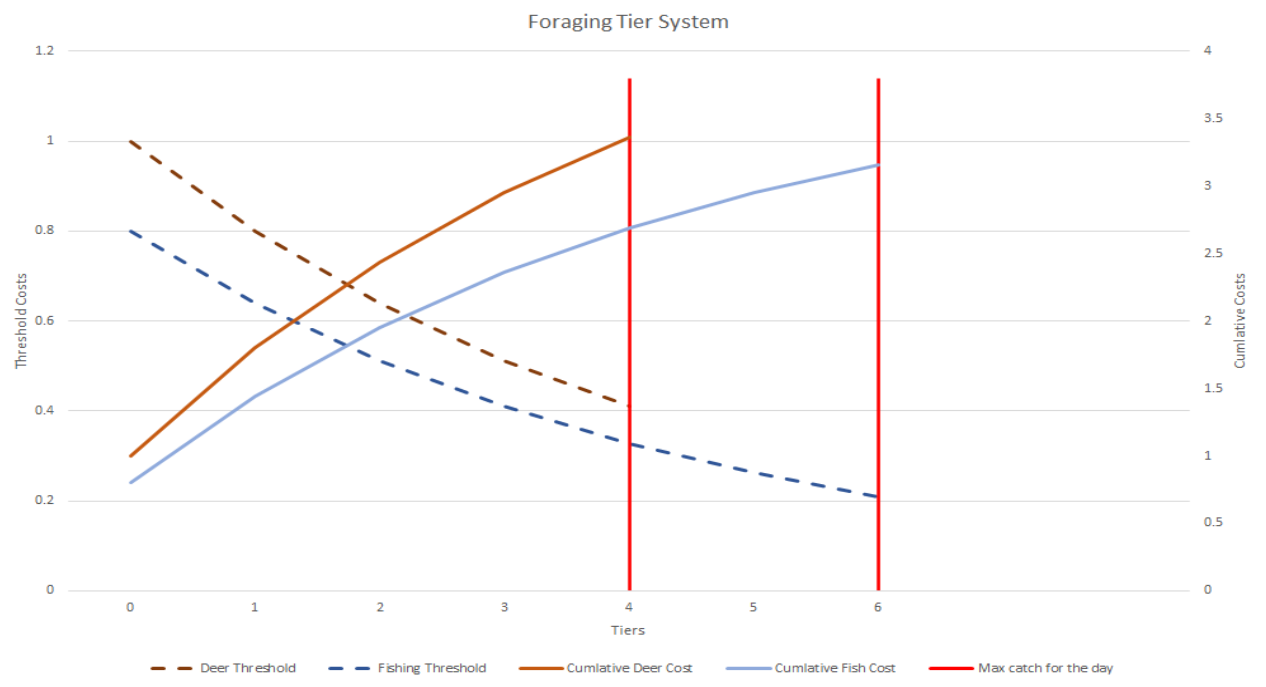
\includegraphics[width=0.9\textwidth]{04_environment/Images/Foraging Tier System.PNG}
    \caption{Foraging Tier System}
    \label{Images:Foraging Tier System}
\end{figure}

As the tiers increase the cost per animal decreases but the total cost increases up to a daily catch limit. Thus if teams collaborate, they could invest less as individuals to get a good return through deer hunting, however if they invest too much then they will over spend as they reach the daily max catch. Thus it would be beneficial for some teams to go fishing which has a higher maximum catch per day but comes with lower returns (thus there is a need for some self sacrifice to be done to reach maximum welfare). \\ 

Fishing has similar functions with the key difference being the Tiers start at 1 and Normal distribution. \\

\newpage
\subsection{Examples Distributions}
\subsubsection{Example of the distribution for foraging return (Deer hunting - payoff dominant)}

\begin{figure}[!htb]
    \centering
    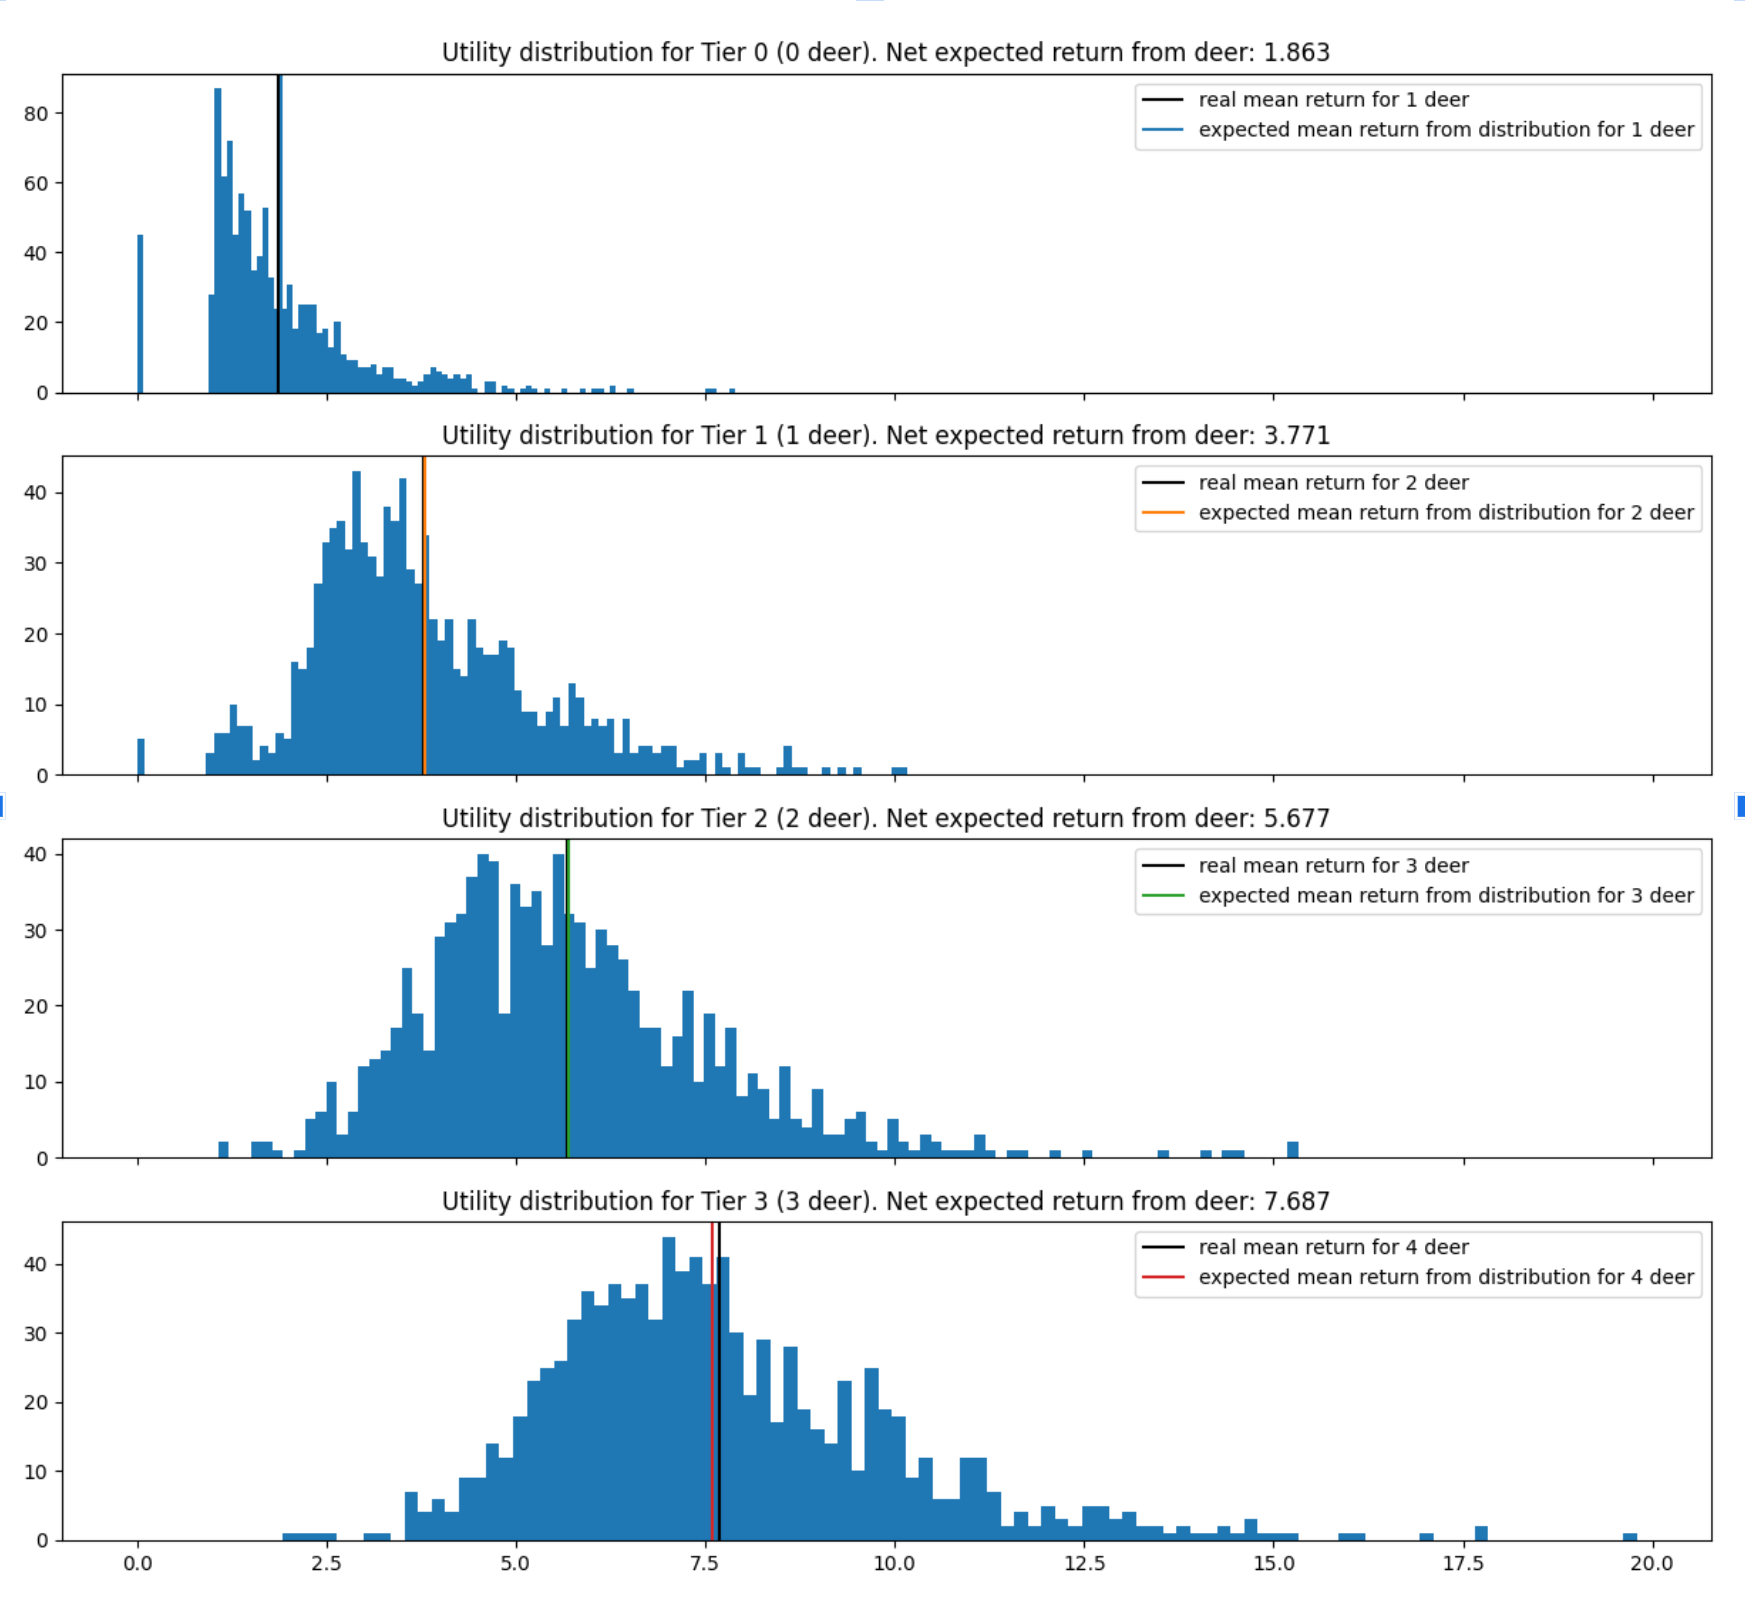
\includegraphics[width=1\textwidth]{04_environment/Images/Distribution of Foraging returns Deer Hunting.PNG}
    \caption{Deer hunting payoff dominant Distribution for foraging return}
    \label{Images:Distribution of Foraging returns Deer Hunting}
\end{figure}

To increase the risk we have used a Bernoulli Random Variable (D) that makes it possible for the hunt to not return any resources. Whilst the Exponential Decay (W) is to disincentive too much resources being placed in hunting and hoping for a high return. However this all comes with the benefit of significantly higher (2x) returns than fishing.\\ 

The above graph represents the return utility which represents the return multiplier of the foraging. The average \textbf{expected mean} return across 1000 iterations is shown by the colourful lines which is close to the \textbd{real mean}.\\

\newpage
\subsubsection{Fish hunting - risk aversion}

Fishing is similar to Deer hunting, except that it uses only a Normal Distribution (F), which focuses on avoiding risk by being very predictable and safe. The Figure below illustrates the return utility function of fishing.\\

\begin{figure}[!htb]
    \centering
    \includegraphics[width=1\textwidth]{04_environment/Images/Distribution of Foraging returns Fishing.PNG}
    \caption{Fishing Risk aversion Distribution for foraging return}
    \label{Images:Distribution of Foraging returns Fishing}
\end{figure}

As seen in the graphs the return for the deer is almost double that of the fish return whilst the fish return is much easier to obtain due to the lower cost of catching fish. \\

\newpage
\subsection{Solution Concepts}
\subsubsection{Dominant Strategy}

In our implementation there is no dominant strategy as picking deer hunt when other players switch to fishing could lead to significantly worse returns due to insufficient resources. Whilst picking fish hunt when enough resources are invested in deer hunting will net you a worse return than if you went deer hunting.\\

\subsubsection{Nash Equilibrium}

In the regular stag hunt game there are 2 pure Nash equilibria, where both players go for either payoff or risk aversion. In our implementation there are multiple Nash Equilibria; these would be the points where the islands cannot benefit themselves by moving to deers hunting to generate more return. As there is a limit to how many deers that can be hunted thus by moving to deer hunting they are getting a worse return than if they just stayed at fishing. Whilst the islands at the deer hunt are already making a greater return and have no reason to switch to fishing.\\ 

\subsubsection{Pareto Optimal Strategy}

At some point all players will be in a position where changing foraging methods will not yield any better income for themselves and in fact also hinder others. This is due to the max daily deer hunt limit which will create a maxim return on the deer hunt. Therefore there will be points where the islands will change as the amount of resources being entered into both methods of foraging is the most efficient, this being where deer returns are maximised. There may also be a point where the user can benefit by switching away from deer hunting, however this will cause the other islands in the deer hunt to have a worse pay off due to a possible drop in tier resulting in worse returns.\\

\begin{figure}[!htb]
    \centering
    \includegraphics[width=0.7\textwidth]{04_environment/Images/Pareto Optimal Strategy.PNG}
    \caption{Pareto Optimal Strategy}
    \label{Images:Pareto Optimal Strategy}
\end{figure}

\subsubsection{Social Welfare Maximisation}

It is possible for these islands to find the social welfare maximum in this foraging function with enough time. The islands could identify the exact amount of resources needed, for both fishing and deer hunting, to achieve the best return according to the maximum number of animals. Thus by cooperating who goes where and spends how much they are able to maximize their returns without spending more resources than necessary.\\

\subsection{Extended Work}

For the future implementations, our additions focus on further exploring the dynamics of our agents and allowing for a more complex decision-making interaction between clients and the environment. Some of these design ideas were later implemented in self-organising multi-agent system and others are expressed for the sake of completeness and future work recommendations.\\

Some changes have been made to make foraging more volatile and unpredictable. These will add to the complexity of the system, allowing the teams to further evaluate the clients’ performance on observing and using learned knowledge to take action.\\

\subsubsection{Incorporated Changes: Population density}

Introducing a model that controls the population density of deer allows us to increase the complexity of the foraging function. In short, the deer hunting capacity decreases with decreasing population and increases with an increasing population. This will then influence the maximum deer per hunt parameter(n), which in turn results in a more complex return calculation function (\texttt{\textbf{DtotalReturn}}), which would make it harder for agents to figure out forage tier boundaries to optimise their strategies.\\

The population change can be dynamic depending on various environmental factors, fetched from the rest of the system. For example, a Disaster could supposedly cause the population density of deer to halve, making it harder to forage and therefore, causing lower returns. For future implementations, the team uses a single species population model and more specifically logistic modelling for the deer and fish population. The model can be described in the equation below.\\

\begin{equation}
\frac{\mathrm{d} P}{\mathrm{~d} t}=k(N-P)
\end{equation}

\begin{itemize}
        \item “P” is the total Population \item “N” is the maximum deer/fish population (“carrying capacity” formally)
        \item “k” is the growth coefficient
        \item “t” is time
    \end{itemize}

In our implementation \textbf{“k”} and \textbf{“N”} are constants but it would be interesting to see what would happen if we were to increase the growth coefficient, causing a population growth and observing the islands’ dynamics. Will they keep on “investing” higher resources each turn, taking advantage of the deer/fish abundance, or will they stick to their original, safe and static strategy?\\

Below, we can see a simulation of the implemented logistic model, with a growth coefficient of 0.2 and \textbf{“N”} of 8. It can be seen that overtime there is an unpredictable pattern to population changes, which would be interesting to see affecting the tier system and in extend, the deer/fish foraging strategies of the agents.\\

\begin{figure}[!htb]
    \centering
    \includegraphics[width=1\textwidth]{04_environment/Images/Deer population over time.PNG}
    \caption{Deer population over time (turns) under Logistic modelling with a growth coefficient of 0.2.}
    \label{Images:Deer population over time}
\end{figure}

Modelling the population (or linking it to other environmental elements) allows us to make sure that the system’s dynamics are varying, making it harder for islands to settle onto a single foraging method because it always results in better returns. Pareto optimality is therefore harder to achieve and thus maximising social welfare is trickier, requiring agents to make more informed decisions, recognizing possible patterns. Of course, that would be an easier task for the islands, if they had knowledge on what is affecting the population (i.e. disasters), whereas a logistic model function might be more abstract in the eyes of our agents, requiring more processing. \\

\subsubsection{ Incorporated Changes: Method of resource allocation}

Lastly, in future implementations, a parameter can be set that allows either an equal split of returns after foraging no matter the input, or a proportional split that is dependent on the amount of resources inputted by each island. Both of these implementations work in accordance to the previous specification. Such change will allow us to observe the concept of free-riding further, looking at how greedy islands behave in the case of uniform resource returns. Will the islands seek to minimise inputs and benefit from the more generous islands, even at the cost of being allocated a lower tier? Will they input just enough to maximise the tier they are foraging in? Or, will they observe other island’s previous contributions and make a decision based on that? These are some of the questions we can later explore using this future change. \\

\subsection{Future Work Concepts}

For the Future implementations, our additions focus on further exploring the dynamics of our agents and allowing for a more complex decision-making interaction between clients and the environment. Some of these design ideas were later implemented in self-organising multi-agent system and others are expressed for the sake of completeness and future work recommendations.\\

Some changes have been made to make foraging more volatile and unpredictable. These will add to the complexity of the system, allowing the teams to further evaluate the clients’ performance on observing and using learned knowledge to take action.

\subsubsection{Incorporated Changes: Population density}

Introducing a model that controls the population density of deer allows us to increase the complexity of the foraging function. In short, the deer hunting capacity decreases with decreasing population and increases with an increasing population. This will then influence the maximum deer per hunt parameter(n), which in turn results in a more complex return calculation function (\texttt{\textbf{DtotalReturn}}), which would make it harder for agents to figure out forage tier boundaries to optimise their strategies.\\

The population change can be dynamic depending on various environmental factors, fetched from the rest of the system. For example, a Disaster could supposedly cause the population density of deer to halve, making it harder to forage and therefore, causing lower returns. For future implementations, the team uses a single species population model and more specifically logistic modelling for the deer and fish population. The model can be described in the equation below.\\

\begin{equation}
\frac{\mathrm{d} P}{\mathrm{~d} t}=k(N-P)
\end{equation}

\begin{itemize}
        \item “P” is the total Population \item “N” is the maximum deer/fish population (“carrying capacity” formally)
        \item “k” is the growth coefficient
        \item “t” is time
    \end{itemize}

In our implementation \textbf{“k”} and \textbf{“N”} are constants but it would be interesting to see what would happen if we were to increase the growth coefficient, causing a population growth and observing the islands’ dynamics. Will they keep on “investing” higher resources each turn, taking advantage of the deer/fish abundance, or will they stick to their original, safe and static strategy?\\

Below, we can see a simulation of the implemented logistic model, with a growth coefficient of 0.2 and \textbf{“N”} of 8. It can be seen that overtime there is an unpredictable pattern to population changes, which would be interesting to see affecting the tier system and in extend, the deer/fish foraging strategies of the agents.\\

\begin{figure}[!htb]
    \centering
    \includegraphics[width=0.8\textwidth]{04_environment/Images/Deer population over time.PNG}
    \caption{Deer population over time (turns) under Logistic modelling with a growth coefficient of 0.2.}
    \label{Images:Deer population over time}
\end{figure}

Modelling the population (or linking it to other environmental elements) allows us to make sure that the system’s dynamics are varying, making it harder for islands to settle onto a single foraging method because it always results in better returns. Pareto optimality is therefore harder to achieve and thus maximising social welfare is trickier, requiring agents to make more informed decisions, recognizing possible patterns. Of course, that would be an easier task for the islands, if they had knowledge on what is affecting the population (i.e. disasters), whereas a logistic model function might be more abstract in the eyes of our agents, requiring more processing. \\

\subsubsection{ Incorporated Changes: Method of resource allocation}

Lastly, in future implementations, a parameter can be set that allows either an equal split of returns after foraging no matter the input, or a proportional split that is dependent on the amount of resources inputted by each island. Both of these implementations work in accordance to the previous specification. Such change will allow us to observe the concept of free-riding further, looking at how greedy islands behave in the case of uniform resource returns. Will the islands seek to minimise inputs and benefit from the more generous islands, even at the cost of being allocated a lower tier? Will they input just enough to maximise the tier they are foraging in? Or, will they observe other island’s previous contributions and make a decision based on that? These are some of the questions we can later explore using this future change. \\

Further work could be done to make sure that there is enough complexity to explore the dynamics of our agents. Due to the project’s time constraints, some interesting ideas were not implemented but were thoroughly examined during the design process.\\

An important add-on to our previous implementation could be the enforcement of laws by the IIGO for the number of islands that can go foraging. That would introduce the need of internal client relationships, adding another level of decision-making complexity to the agents. The specific alteration could result in some interesting findings. For example, there could be an auction scenario where islands would bid with their input resources, where only the highest bidders would be able to forage, as limited by the IIGO. Therefore, Islands with the lowest resources would be out-bidded, possibly causing a long-term resource depletion that would need to be mitigated by the more resourceful islands later in the game. It would be interesting to see how such change would affect the free-rider problem and how islands would adjust their strategies to out-bid other islands.\\

Another change that could be made, is to let islands choose who they can forage with. That could be in the form of direct messaging or voting. Essentially, our speculation is that agents would avoid the free-riding problem in both cases by enabling agents to make collective decisions based on communicated resource contributions. That’s because free-riders would be out-voted or not invited for foraging. That, in combination with the aforementioned tier system, would possibly result in all the islands contributing as much as possible to the input foraging “pool”.  However, it would be interesting to see if islands can then reach Pareto optimality, where every single agent gets the best possible return for their input.\\

In addition to the above suggestions, area limited foraging where agents would only be allowed to forage with only one neighbouring island using a ranking algorithm. This could also be enforced and implemented in a future iteration. Moreover, this particular scenario could be extended by programming prey densities to be geofocused, where prey populations could vary between regions on the “map”. Islands would then need to make a strategic plan on how their ranking of neighbouring islands would change in accordance to their returns and returns broadcasted from other island pairs.\\

Finally, more foraging options could be added in future implementations. For example, a third foraging technique, call it whale it hunting, could be created. That would have an even higher return than the deer hunting, deeming it an appealing forage method. The barriers of entry could be similar to that of the deer hunting method in this scenario but at the same time, there would be a more spaced out/expensive tier system. This combination would potentially incentivise cooperation between islands, if their strategy was to maximise returns. Also, as we have introduced more foraging methods, it could be the case that we hard-fix the type of return for each method and observe how agents decide to behave. For example, we could have the deer and fish hunting methods result in returns proportional to inputs, whereas the whale hunting method would result in an equal split of returns between all participating islands. Would this mean that islands choose a fairer division of returns and not go on whale foraging at all? Or Would they be intrigued by the higher costs and choose whale hunting over the other foraging methods? In the latter question agents would need to take in mind that an island may be entering an insignificant amount reaping however, a large reward. It is therefore up to the islands to decide if the higher payoff is worth the risk of other islands free-riding.\\

All of the aforementioned behaviours are of course influenced by island tactics and therefore, an island programmed to be greedy will not cease to be greedy no matter how the surrounding islands’ behaviours change, unless the greedy island can adapt. Therefore, conclusions drawn on specific foraging methods, and how agents react with them, need to take this into account.\\

\section{Disaster}
\subsection{Disaster Background}

A game has been designed, where agents are at risk, they will be directly confronting a risk/a disaster once every round. This subset of the game creates a dilemma, where each island (agent) has to survive. They will have the opportunity to work together by investing collectively to the common pool, the disaster will be mitigated if the islands invest enough resources to reach a desired threshold. Otherwise, the islands would face negative impact, which would diminish their available resources. It is worth mentioning that the disaster will first extract resources from the common pool, and then if not enough resources have been invested, resources will be depleted from each island proportionally to their island’s damage.\\

Furthermore, the disaster has been designed to comprise of an epicentre (eye of the storm), which is limited within the archipelago bounds, it is represented using Cartesian coordinates (EpiX, EpiY). Therefore, all islands or a subset of islands may be affected due to their proximity to the disaster epicentre. The island’s proximity to the disaster epicentre is directly proportional to the island’s damage. In other words, the island's available resources will be diminished based on the disaster magnitude and its location with respect to each island’s fixed location.\\

The following example can briefly explain the dilemma:\\

The closest an island from the eye of the storm, the larger the severity on that island. Therefore, the more resources are depleted. Let’s say that the disaster epicentre hits around island 1 as shown in Figure below. and that the desired common pool threshold has not been met. Island 1 would be experiencing severe damages , and island 2 and 6 some damages and the other islands low to no damage. Therefore, Island 1,2 and 6 have the risk of not surviving if they are lacking resources, whereas island 3, 4, and 5 would not be affected as much by the disaster.

\begin{figure}[!htb]
    \centering
    \includegraphics[width=1\textwidth]{04_environment/Images/Disaster eye of the storm severity.PNG}
    \caption{Disaster Epicenter effects}
    \label{Images:Disaster eye of the storm severity}
\end{figure}

\newpage
\subsection{Functions within the Disaster}
It is worth mentioning that the island's geography in infrastructure is the combination of the island number and the island’s fixed location in the archipelago.\\

\begin{table}[h]
\begin{center}
\begin{tabular}{|p{1.1in}|p{1.1in}|p{1.1in}|p{1.1in}|} \hline
\textbf{Functions} & \textbf{Description} & \textbf{Inputs} & \textbf{Outputs} \\ \hline
\textit{Bernouilli Distribution \texttt{(pdfGlobal)}} & Whether a disaster is going to occur & -The probability of a disaster occurring,\newline -The Global probability variable & Determines the likelihood of a disaster occurring \\ \hline
\texttt{PdfMag} & Exponential distribution & -The spatial PDF & Determine the disaster magnitude \\ \hline
\texttt{Epix,EpiY} & Spatial probability distribution function & -The spatial PDF\newline -Disaster Magnitude & Determines the location of the disaster epicentre \\ \hline
\texttt{DisasterEffect} & Island's Proximity distance to the eye of the storm & -Island geography\newline -Eye of the storm location & Determine the islands damage \\ \hline
\end{tabular}
\caption{\label{tab:table-name}Disaster's main functions}
\end{center}
\end{table}

The disaster has been computed as part of the infrastructure: Each island has a fixed position, characterised using Cartesian coordinates. They are located in the archipelago which captures the collection of island geographies including the bounding regions of the entire archipelago.\\

Furthermore, to determine when a disaster is going to occur, we have used the Bernoulli random variable (probability of a disaster occurring is low).\\

The Spatial probability distribution function "Spatial PDF" is uniform and it controls the distribution works of XY grid of the location of the disaster. The magnitude is then exponentially distributed (it exponentially more likely to have a smaller magnitude as we want large disasters to be more rare, occur less frequently). In addition, we have created a magnitude variable "Lambda" which can vary the slope of the exponential function (create a harsher environment when increasing the "lambda variable" by creating larger disasters and vice versa). In addition, the eye of the storm (disaster epicentre) is limited within the bounds of the environment (The environment bounds are fixed, they are specified by the users).\\

\begin{figure}[!htb]
    \centering
    \includegraphics[width=1\textwidth]{04_environment/Images/Disaster output infrastructure.png}
    \caption{Infrastructure Disaster outcome}
    \label{Images:Disaster output infrastructure}
\end{figure}

The image above illustrates the output of the disaster, it first shows the magnitude of the disaster and the precise location of the eye of the storm, it indicates as well the fixed location of each island as well as the proportional effect of each island. For example, Island 2 with a fixed location of (5,0) has the largest disaster effect, which means it is the closest to the eye of the storm.\\

\subsection{Future works Concepts}

The disaster is a random function, meaning that it is possible to predict it with the current game.\\

There are multiple future works ideas that would be developed in the design aspect such as; a deterministic disaster which would be  designed as a straight line that accumulates during the days, once the threshold has been met then the disaster would occur. Another deterministic disaster idea would be to link the disaster’s magnitude to time. Thus, agents will have to learn from past disaster occurrences, creating a memory. Agents will start learning from past disasters and will be able to forecast the next one. Therefore, the agents will be able to forecast that if a disaster did not surface for a long period of time, then the magnitude of the next disaster will be much larger than the previous one.\\

Another Idea is that agents can invest into forecasting. Therefore, agents will have access to a history of past disasters, which would be utilised by the agents to learn and gain knowledge in order to predict the upcoming disaster. The larger the amount of resources invested; the agents will have access to a larger history of previous disasters. Therefore, agents will acquire knowledge, when investing resources.\\

\section{Common Pool}
\subsection{Common Pool Background}

We are designing a game where 6-islands (agents) are having access to a common-pool resource. In micro-level, each island intends to maximise its utility while in macro-level, all the islands want to maintain sustainability and be protected by the upcoming disaster. The above description specifies a collective action problem where n-agents (6 in our case) are seeking access to a common pool resource that is sufficient to satisfy some agents but not to satisfy all of them.\\

We have implemented a Linear Public Goods (LPG) Game where all the agents individually own some resources and try to maintain and increase them, by foraging, but also contribute a part of them to the common pool. This common pool is used for the payment of expenses of the institutional roles and for the protection towards the disaster.\\

In more detail, the common pool is represented by a structure with following characteristics:

\begin{itemize}
    \item Common Pool Threshold
    \item Amount of Resources 
\end{itemize}

According to the specifications of an LPG Game, the agents should be able to perform the following actions:  

\begin{itemize}
    \item Request Resource from the Common Pool 
    \item Contribute Resource to the Common Pool 
\end{itemize}

And the Common Pool is responsible for two more actions: 

\begin{itemize}
    \item Mitigate Disaster
    \item Deplete islands after a disaster
\end{itemize}

\newpage
\subsection{functions within the Common pool}

For each of these action a relevant function has been implemented as follows:\\

\begin{table}[h]
\begin{center}
\begin{tabular}
{|p{1.1in}|p{1.1in}|p{1.1in}|p{1.1in}|} \hline
\textbf{Name} & \textbf{Description} & \textbf{Input} & \textbf{Outcome} \\ \hline
\texttt{islandDistribute} & Distribute Resources from Common Pool to Island upon Request & -Requested Amount of Resources\newline -Island Name & Resources subtracted from CP and added to island \\ \hline
\texttt{islandContribute} & Contribute Resources from Island to Common Pool & -Donated Amount of Resources\newline -Island Name & Resources subtracted from Island and added to CP \\ \hline
\texttt{DisasterMitigate} & Mitigate the Disaster with the Amount of Resources in the Common Pool & - Effect of Disaster to each island\newline - Proportional effect of Disaster to each island (magnitude of disaster divided by the distance of the island from epicenter) & Resources in CP were exploited for the mitigation of the disaster and remaining effect has to be mitigated by each island \\ \hline
\texttt{islandDeplete} & Deplete Islands after the disaster (with the amount of disaster that couldn't be mitigated by CP) & -Remaining effect for each Island\newline -List of Islands & The remaining proportional effect of the disaster to each island is causing the depletion of resources \\ \hline
\end{tabular}
\caption{\label{tab:table-name}Common Pool's main functions}
\end{center}
\end{table}

The common pool has been computed as part of the infrastructure: with a threshold that is the amount of resources to hopefully help to completely mitigate the disaster. If the threshold is met, the damage from the disaster on the common pool and islands will be half the actual amount. This incentivises islands to contribute to the common pool and reflect the reality that, if there is enough preparation for the disaster, the damage will be much less compared to no preparation. Furthermore, it is worth mentioning that the threshold is a fixed value.\\

Another important input to the implementation is the magnitude of the disaster’s damage to each island. As shown in Figure 1.9 , the disaster’s magnitude is 3.458. However, the disaster’s effect on individual islands do not add up to 3.458 because the storm’s epicenter is further away from the islands. This aspect creates a more realistic scenario to the game. From the islands’ individual damage, proportional effects are calculated to determine which island has been hit harder out of the 6 islands. The summation of these proportional effects is equal to 100\%, which is the total effective damage. \\

If the common pool has enough resources to fully mitigate the disaster, the process is very easy. However, in the unfortunate events, the common pool resources will be used to mitigate each island's damage according to their proportional effect i.e., if an island is hit harder, it will receive more help from the common pool. This is also visualized in Figure 1.9, as island 4 withstands most damage from the storm, the common pool gave island 4 most help with 252.47 resources (“common pool mitigated” column). The updated damage value shows the leftover damage of the disaster that the common pool was not able to mitigate. These leftover damage will be used to further deplete the island's private pool of resources. If there are enough resources in the common pool totally mitigate the disaster then the update damage values will be 0.\\

\begin{figure}[!htb]
    \centering
    \includegraphics[width=1\textwidth]{04_environment/Images/Common Pool infrastructure outcome.PNG}
    \caption{Demonstration of how common pool works in software}
    \label{Images:Common Pool infrastructure outcome}
\end{figure}

The common pool threshold is a fixed value and known to islands. later, the functionality of making the Threshold unknown to the islands would be added. \\

The common pool resources will be given to each island based on the severity of the damages.\\

If the amount of resources in the common pool exceeds the total effect of disaster, then the leftover amount of resources in the common pool will be used for the next round.\\

Since the goal of each island is to maximise its utility, the following dilemma shows up: islands can free ride by not contributing to the common pool and yet receiving the benefits after a disaster or if they are aware that they would not be depleted by the disaster - since they are far away from the eye of the storm - they might also not contribute to the common pool and thus the rest of the islands would be severely destroyed. \\

The following example can briefly explain this dilemma:\\

If the epicentre of disaster is known to the islands and happens to coincide with the location of Island 1, then Island 4 might not contribute at all to the CP since it will not be affected by the disaster. Moreover, Islands 3 and 5 that will not be severely hit might contribute a small amount to the CP or even zero amount (free riding case). Since the rest of the islands might contribute to the CP, then Islands 3 and 5 will be profited by the contribution of others.\\

We wanted to highlight the importance of prevention and incentivise islands to contribute to the Common Pool, thus if the amount of resources in the common pool exceeds the threshold when the disaster happens, then the “power” of disaster towards the islands and common pool will be decreased. It makes sense in real life, as more preparation will result in less damage. The actual damage of disaster is decreased by half, but this can vary later.\\

\subsection{Example distribution}
This can be described by the examples in table X, which shows 4 possible scenario:\\ 

\begin{itemize}
    \item Contribution to common pool does not meet threshold and common pool cannot fully mitigate disaster’s damage
    \item Contribution to common pool does not meet threshold but common pool can fully mitigate disaster’s damage
    \item Contribution to common pool meets threshold but common pool cannot fully mitigate disaster’s damage
    \item Contribution to common pool meets threshold and common pool can fully mitigate disaster’s damage
\end{itemize}

\begin{table}[h]
\begin{center} 
\begin{tabular}{|p{0.9in}|p{0.9in}|p{0.9in}|p{0.9in}|p{0.9in}|} \hline
& \textbf{Scenario 1} & \textbf{Scenario 2} & \textbf{Scenario 3} & \textbf{Scenario 4} \\ \hline
\textbf{Disaster total damage} & 1000 & 200 & 1200 & 1200 \\ \hline
\textbf{CP's threshold} & 500 & 500 & 500 & 500 \\ \hline
\textbf{CP's current value} & 300 & 300 & 500 & 700 \\ \hline
\textbf{CP's multiplier} & 1 & 1 & 0.5 & 0.5 \\ \hline
\textbf{Mitigated damage} & 300 & 200 & 500 & 1200 \\ \hline
\textbf{Remaining damage} & 700 & 0 & 100 & 0 \\ \hline
\textbf{CP's remaining value} & 0 & 100 & 0 & 100 \\ \hline
\end{tabular}
\caption{\label{tab:table-name}Demonstration of how common works in different scenarios}
\end{center} 
\end{table}

In scenario 1, the disaster total damage is high, however there is no preparation from the islands through contribution to the common pool. As a result, the common pool could not mitigate all of the damage and 70\% of the damage will be directly on the islands\\

In scenario 2, even though there is no preparation, the common pool is still able to mitigate all of the damage thanks to the low damage of disaster. The leftover resource in the common pool will stay there.\\

In scenario 3, the disaster damage is high. Fortunately, the islands have prepared themselves moderately through contribution to the common pool. Thus, the islands only have to take very little leftover damage.\\

In scenario 4, the disaster damage is high and the islands have prepared themselves very well. As a result, the damage is fully mitigated by the common pool and there is still leftover resource in the pool. 


\subsection{Future Works Concepts}
To observe behaviors of agents in different settings, the future works of the common pool will be centered around varying the values of different parameters such as threshold and threshold multiplier. The forecasting function of the disaster part can be used as a tool to variate the common pool’s threshold and multiplier accordingly. In events that damage could be high, the preparation should be done more carefully, thus the common pool’s threshold can be raised to let islands know about potential damage from disaster. The same thing can be done for threshold multiplier, where the multiplier will be greater for bigger disaster. Since threshold and multiplier both encourage the preparation for disaster, one of them can be fixed at certain seasons to observe different behavior of agents when it comes to varying different parameters. 

    \chapter{Inter-Island Governmental Organisation (IIGO)}


The role of IIGO is to maintain, update, and revise the rules concerning provision to managing the long-term collective risk dilemma (ltCRD). 

\begin{itemize}
    \item There will be 3 distinct branches in the IIGO: the \textbf{legislative branch}, \textbf{executive branch} and \textbf{judicial branch}\footnote{This is, as no surprise, inspired by the separation of powers in Western democracies.}.
    \item Each role is put in power according to the  transfer-of-power rules (see Section~\ref{subsec:transfer-of-power} for more detail).
    \item The head of the legislative branch is the Speaker, the head of the executive branch is the President, and the head of judicial branch is the Judge.
    \begin{itemize}
        \item  The Speaker, President and Judge are selected, through a democratic election, from the islands in the archipelago\footnote{This naming is inspired by the roles in the US Government.}.
        \item The resources gathered by the archipelago are endogenous, hence acting on the institutional powers granted to the Speaker, President or Judge costs resources. 
        \item For their duty, the President, the Speaker and the Judge receive a salary for each of their turns in office (see Section~\ref{subsec:salary} for more detail).
        \item The limit of the powers of the President, Speaker and Judge are defined in this chapter (e.g. the Speaker can only call one vote per turn).
 
    \end{itemize}
\end{itemize}

\subsection{IIGO Specific Definitions}
\begin{definition} \label{def:ballot}
    A \textbf{ballot} is related to each island's \textbf{power} to support or disagree with the rule specified in the vote called by the President and to vote in favour or against an island for a specific role (i.e. the President, Speaker, Judge) at each round of the game.
\end{definition}


%\begin{definition} \label{def:vote}
    %A \textbf{vote} is related to a role's (i.e. the President, Speaker, Judge) \textbf{power} to call a vote for a specific rule or an election.
%\end{definition}


\begin{definition} \label{def:tax}
    The \textbf{taxation} is related to the President's \textbf{power} to request a specific \underline{\textbf{minimum}} amount of contribution from each island to the common pool at each round of the game. 
\end{definition}

\begin{definition} \label{def:alloc_req}
    An \textbf{allocation request} is related to each island's \textbf{power} to request a specific amount of resource allocation from the President at each round of the game.
\end{definition}


\begin{definition} \label{def:rule_prop_list}
A \textbf{rule proposal list} is related to each island's \textbf{power} to propose a specific rule to be passed to the President at each round of the game.
\end{definition}

\begin{definition} \label{def:invst}
    An \textbf{investigation} is related to the Judge's \textbf{power} to acquire information to make a decision, followed by a calculation of the expected results and checking whether some specific rules have been obeyed, exclusively for the actions carried out by the \textbf{islands}. 
\end{definition}


An example of an \emph{investigation}: The President has permitted the island $X$ to take the amount of $Y$ resources from the common pool. Upon \emph{investigation} carried out by the Judge, it is revealed that the amount of resources taken out from the common pool by the island $X$ is, in fact, $Y'$ such that $Y' \neq Y$.


\begin{definition}
\textbf{Monitoring} is a government official's \textbf{power} to perform event recognition and to check whether some specific rules have been obeyed.
\end{definition}

An example of \emph{monitoring}: The Speaker has performed only the following action: \emph{counted the votes and calculated the result} for a rule. Upon \emph{monitoring} carried out by the President, it is noticed that the Speaker has not made any \emph{announcement}. Hence, the Speaker has not followed their obligation to \emph{announce} the result of any vote held.

See Section~\ref{sec:accountability} for more information about which roles can monitor which ones.


\begin{definition}
\textbf{Investigative-monitoring} is a government official's \textbf{power} to acquire the information used in acting on a governmental power followed by calculation of the expected results and checking whether some specific rules have been obeyed, exclusively for the actions carried out by a government official they are responsible for.
\end{definition}

An example of \emph{investigative-monitoring}: The Speaker has performed the following actions: \emph{counted the votes and calculated the result $R$} for a vote $V$ and \emph{announced} the result $R'$ for the vote $V$. Upon \emph{investigative-monitoring} carried out by the President, it is noticed that $R' \neq R$. Hence, the Speaker has modified the announced result.


\begin{definition}
The \textbf{sanction} is related to the Judge's \emph{power} to punish non-compliant islands when their disobedience is confirmed through investigations at a specific turn.
\end{definition}


\begin{definition}
The (judicial) \textbf{pardon} is related to the Judge's \emph{power} to forgive a non-compliant island at a specific turn.
\end{definition}

\begin{definition}
The \textbf{budget} is the maximum amount of resources a role is permitted to spend from the common pool as it performs its own institutional-power-enabled actions at a specific turn.
\end{definition}


\begin{definition}
The \textbf{salary} is the amount of resources a role is to be given from the common pool as a reward for performing its institutional-power-enabled actions at a specific turn.
\end{definition}

\begin{definition} \label{def:term}
A \textbf{term} is the number of turns an island is \emph{permitted} to hold a role, and after which the responsible role (indicated in the transfer-of-power cycle in Figure~\ref{fig:cycles_in_IIGO}) is \emph{obliged} to initiate transfer-of-power.
\end{definition}

\subsection{\emph{Power}, \emph{Permission} and \emph{Obligation} Distinction}
In the rest of the specifications, we will be specifically using the following three terms to define the actions and responsibilities carried out by the Speaker, President, Judge (see Figure~ \ref{fig:per_obl_sets}):
\begin{itemize}
    \item Power
    \item Permission
    \item Obligation
\end{itemize}



\begin{figure}[H] 
\centering
\includegraphics[width=0.6\textwidth]{05_iigo/images/SOMAS_per_obl.pdf}
\caption{Relationship between \emph{power}, \emph{permission} and \emph{obligation}.}
\label{fig:per_obl_sets}
\end{figure} 


For example, the Judge has the \emph{power} to carry out investigations at an IIGO session. There are no rules specifying which specific islands the Judge should investigate. Therefore, the Judge has the \emph{permission} to investigate any `alive' islands during a session. However, the Judge is \emph{obliged} to make at least some number of investigations each turn.



\section{Executive Branch}
\label{sec:executive}
The executive branch is responsible for \textbf{carrying out the law}.
\begin{itemize}
       
    \item The President has the \emph{power} to: 
    \begin{itemize}
        
        \item Select a rule for voting $R^{*}$ to be passed to the Speaker.
        \begin{rule_IIGO}
            The President has the \emph{obligation} to \emph{select} a rule $R^{*}$ if the \emph{rule proposal list} has at least one proposed rule in it.
        \end{rule_IIGO}
        \begin{rule_IIGO}
            The President has the \emph{permission} to \emph{select} a rule $R^{*}$ if and only if $R^{*} \in S$, where $S$ is the \emph{rule proposal list}.
        \end{rule_IIGO}
        
        \item Decide the amount of individual \emph{taxation} (i.e. a specific \emph{minimum} amount of contribution to the common pool for each island) for the current turn.
        
        \begin{itemize}
            \item The President is given the self-reported resource amounts held by each island to assist in this decision.
            %\item Suggested Rule: For any island that has chosen to not report it's resources, the President has the \emph{obligation} to set them an individual tax amount T.
        \end{itemize}
        
        \item Decide the allocation of resources distributed from the common pool to the islands (i.e. a specific \emph{maximum} amount an island is permitted to take from the common pool).
        
        \begin{itemize}
            \item The President is given the \emph{allocation requests} made by each island.
            %\item \emph{}{Suggested Rule:} The President has an obligation to prioritise islands in critical condition.
        \end{itemize}
    \end{itemize}
\end{itemize}



\section{Legislative Branch}
\label{sec:legislative}
The legislative branch is responsible for \textbf{making the law}.
\begin{itemize}

    \item The Speaker has the \emph{power} to:
    \begin{itemize}
        
        \item Call a vote $V$ for a rule $R$.
        \begin{rule_IIGO}
            The Speaker has the \emph{obligation} to \emph{call} a vote $V$ if and only if the President has \emph{selected} a rule $R$ to be voted on.
        \end {rule_IIGO}
        \begin{rule_IIGO}
            The Speaker has the \emph{permission} to \emph{call} a vote $V$ for a rule $R$ if and only if the rule $R = R^{*}$, where $R^{*}$ is the rule \emph{selected} by the President.
        \end {rule_IIGO}
            
        \item Choose which islands are participating in the vote $V$.
       % \footnote{This is our sequential implementation alternative for the power to close the ballot box.}.
        \begin{rule_IIGO}
            The Speaker has the \emph{obligation} to ask for a vote from all alive islands.
        \end {rule_IIGO}
            
        \item Declare the result $C$ of a vote $V$. 
        \begin{rule_IIGO}
            The Speaker has the \emph{obligation} to \emph{declare the result} $C$ for a vote $V$ if and only if the vote V has been \emph{called}.
        \end {rule_IIGO}
        \begin{rule_IIGO}
            The Speaker has the \emph{permission} to \emph{declare the result} $C$ for a vote $V$ if $C = C^{*}$, where $C^{*}$ is the result produced by \emph{calling} the vote $V$.
        \end {rule_IIGO}
        \begin{itemize}
            \item This step is what enables a rule to be \emph{active}.
        \end{itemize}
    \end{itemize}
\end{itemize}




\section{Judicial Branch}
\label{sec:judicial}

The judicial branch is responsible for \textbf{evaluating the law}.
\begin{itemize}
    \item The Judge has the \emph{power} to:
    \begin{itemize}
        \item Perform a number of \emph{inspections}\footnote{An \emph{inspection} \textbf{costs} an expense of resources (See Definition~\ref{def:invst} for more detail).} $I$ and produce a compliance outcome $\mathbb{O}^{*}$\footnote{Note that the compliance outcome $\mathbb{O}^{*}$ considered is a boolean.}.
        %(true: the island has been compliant with the rules in play, false: the island has not been compliant with the rules in play)
        %\begin{itemize}
           % \item For example, to check if the event outcome is \emph{concurrent}\footnote{Again, what is defined as "concurrent"? A clear definition is needed.} with the rules.
        %\end{itemize}
        \begin{rule_IIGO}
            The Judge has the \emph{obligation} to make at least $N$ investigations at each turn.
        \end{rule_IIGO}
        \item Declare the outcome $\mathbb{O}$ of an inspection $I$ to all islands\footnote{This act of broadcasting is especially important for islands to form an opinion about the sanctioned islands accordingly.}.
        \begin{rule_IIGO}
            The Judge has the \emph{obligation} to declare the outcome $\mathbb{O}$ of an inspection $I$ if and only if the inspection $I$ has been performed.
        \end{rule_IIGO}
        \begin{rule_IIGO}
            The Judge has the \emph{permission} to declare the outcome $\mathbb{O}$ of an inspection $I$ if $\mathbb{O} = \mathbb{O}^{*}$, where $\mathbb{O}^{*}$ is the outcome of the inspection $I$.
        \end{rule_IIGO}
        %\item Initiate the removal of the \texttt{President}.
        %\begin{itemize}
            %\item A good Judge would be especially vigilant during \emph{power transfer} regarding the \emph{President} position (see Section~\ref{leg_const} for more detail).
        %\end{itemize}
        \item Invoke economic \textbf{sanctions} (see Section~\ref{sec:sanctions} for more detail).
        \begin{rule_IIGO}
            The Judge has the \emph{obligation} to invoke a sanction $S$ for an island $X$ if and only if an investigation $I$ has an outcome $\mathbb{O}^{*}$ indicating non-compliance, and $I$ is an investigation of an action taken by island $X$.
        \end{rule_IIGO}
        \item Invoke even more severe sanctions in the case of further disobedience to previous sanction(s).
        \begin{rule_IIGO}
            The Judge has the \emph{permission} to invoke a severer sanction $S'$ for an island $X$ if the island $X$ has not fulfilled the requirements of the previous sanction $S$.
        \end{rule_IIGO}
        \item Pardon the islands which are currently sanctioned.
        \begin{rule_IIGO}
            The Judge has the \emph{permission} to revoke any sanction $S$ of an island $X$ at a specific turn.
        \end{rule_IIGO}
    \end{itemize}
\end{itemize}
%(e.g. a new rule that falls under a "sanction" category \hl{[I'm not sure about this being a `new rule` [Ezgi]]}

\subsection{Sanctions}
\label{sec:sanctions}
All sanctions are of economic nature which include:
        \begin{itemize}
            %\item Revoking an island's access to the common pool.
            \item Enforcing an island to contribute a specific amount of resources to the common pool.
            \begin{itemize}
                \item This does not mean that the Judge has the \emph{power} to take resources from an island in order to put them to the common pool -- the island itself is expected to carry out this implication imposed by the sanction itself, otherwise further punishment can be induced by the Judge.
                \item Similarly, \emph{opinion formulation} will follow accordingly whether the island(s) is/are following the implications imposed by the sanction(s).
            \end{itemize}
        
    \end{itemize}
    Sanctions are the associated penalty that comes with an island breaking a specific rule. The Judge is in full control of the penalties associated with breaking any rules. Once the Judge has specified the score of the penalty associated with each time an island breaks a rule, the cumulative penalties accumulated by the island are then used to determine which \textbf{sanction tier} that each island falls into. The score threshold to determine the boundaries of the sanction tiers are set by the Judge. At each turn of the game, each island is told whether they are being sanctioned, and if so, which \textbf{sanction tier} that they are currently in. The \textbf{sanction tiers} of the non-compliant islands are also broadcasted to the other islands in the archipelago. To summarise, the sanctioning process follows these steps:
    
    
    
    %Sanctions are based on an island breaking a rule. Each rule must therefore have an associated penalty. By default, we set these penalties such that they add $1$ to the total sanction score for each island. However, we allow the judge to override this scoring, the judge is able to set their own scores for any particular rule as they desire. This custom scoring is then used when an island breaks a particular rule. By looking at events that occurred in the last turn, and using the customised scoring we provide the holder of the judge role with full control of the penalties for breaking any rules.
    
    





%we then use the cumulative penalties accumulated by each island to determine which Sanction Tier they fall into. The score threshold's required to fall into these sanction tiers is set by the judge and is checked for monotonicity. Each island is told whether they are being sanctioned, and is so what tier they are in. We also tell other islands about which sanction tiers other islands have fallen into. 

    \begin{enumerate}
        \item The Judge has the \emph{power} to set custom penalties associated with breaking any rules.
        \item The Judge is given a list of all events that occurred in the previous turn.
        \item The Judge has the \emph{power} to check whether any, or all of these previous events, involve the islands in the archipelago breaking any rules.
        \item Each of the transgressions is scored using the Judge's custom penalties if the Judge has set them. Otherwise, a score of $1$ is given each time a rule is broken.
        \item The Judge has the \emph{power} to revise the sanction thresholds.
        \item Using the latest sanction thresholds available, each island is assigned to a sanction tier based on the sanction score that it has received.
        \item These sanction tiers are broadcasted to all of the islands in the archipelago.
        \item The Judge then uses sanctions rules in place to calculate the specific amount of resources that each non-compliant island has in order to determine how much it should contribute to the common pool, based on the sanction tier that it is in.
    \end{enumerate}



\section{Constitutional Rights and Obligations in the Archipelago}
\label{sec:const_rights_obl_archi}
Each island has the \emph{power} to:
\begin{itemize}
\item make an \emph{allocation request} (see Definition~\ref{def:alloc_req}) to the President for a specific amount to be allocated to them.
\item report the number of resources it is in possession of to the President.
\begin{rule_IIGO}
    Each island has the \emph{obligation} to report the number of resources it is in possession of to the President.
\end{rule_IIGO}
\begin{rule_IIGO}
    Each island has the \emph{permission} to report the number of resources $R'$ if and only if $R' = R$, where R is the number of resources the island is in possession of.
\end{rule_IIGO}
\item take resources from the common pool.


\begin{rule_IIGO}
    Each island has the \emph{permission} to take at maximum $N$ resources, where $N$ is the specific allocation made by the President to that island\footnote{If no such allocation is made, the island is \emph{permitted} to take any amount of resources.}.
\end{rule_IIGO}
\item contribute resources to the common pool.
\begin{rule_IIGO}
    Each island has the \emph{obligation} to contribute to the common pool an amount greater or equal to that of the individual tax set by the President.
\end{rule_IIGO}
                %The President is in
                %(unless there is a rule in place that dictates how Speaker is to allocate resources).
\item add a rule to the \emph{rule proposal list} (see Definition~\ref{def:rule_prop_list}) at the start of each turn.
        %\begin{itemize}
            %\item The game specification includes how many rules an island can propose each turn.
        %\end{itemize}
        %\item vote  for rules in the Legislative Branch and vote for their favourite islands in elections
\item participate in the legislative branch of the government by casting ballots in votes called by the Speaker
\item vote for an island to be elected for a specific role (e.g. the President, Judge, Speaker) during the elections\footnote{This will be assumed to be true \underline{unless stated otherwise}. %Note that \textbf{diplomatic sanctions} can disable this power of a specific island (see Section~\ref{jud_const}).}.
        }.
\end{itemize}
\section{Accountability Cycle}
\label{sec:accountability}


To ensure that the government avoids corruption and abuse of power, each branch is accountable to another. The President is accountable to the Speaker, the Speaker is accountable to the Judge, and the Judge is accountable to the President (see Figure~ \ref{fig:cycles_in_IIGO}). This accountability cycle is enacted through \emph{monitoring} actions\footnote{Note that the terms \textbf{monitoring} and \textbf{investigation} have similar but quite different meanings in the IIGO context.}. 

The powers related to the accountability cycle and transfer-of-power for each role can be summarized as the following: 
\begin{itemize}
    \item The Speaker has the \emph{power} to: 
    \begin{itemize}
        \item monitor the President.
        \item announce the result of this monitoring.
        \item initiate the transfer-of-power for the Judge.
    \end{itemize}
    \item The President has the \emph{power} to: 
    \begin{itemize}
        \item monitor the Judge.
        \item announce the result of this monitoring.
        \item initiate the transfer-of-power for the Speaker.
    \end{itemize}
    \item The Judge has the \emph{power} to: 
    \begin{itemize}
        \item  monitor the Speaker.
        \item announce the result of this monitoring.
        \item initiate the transfer-of-power for the President.
    \end{itemize}
\end{itemize}

%Unlike investigations performed by the Judge, who performs investigations on island actions in the following turn, each role is given the opportunity to check up on the actions of the role it is responsible for immediately after they have been performed. In this sense, the President can monitor (includes investigative-monitoring) the powers (calling a vote and announcing the result) acted on by the Speaker immediately after the Speaker's announcement (or lack there of). The government officials hold a lot of power so this is to ensure that any wrong-doing is determined as quickly as possible. For this project we are only pursuing one degree of monitoring, that is, the powers relating to the accountability cycle will not be monitored themselves. We assume that agents will act in the interest of themselves and keeping all the islands alive is beneficial to everyone. Hence, while the agents might be inclined to break rules in order to benefit themselves, anyone else breaking the rules is seen as undesirable under the assumption that the system in place is there to benefit all. 


Through the proposed accountability cycle, each role is given the opportunity to check up on the actions of the role it is accountable for immediately after they have been performed. It is clear that the IIGO roles (i.e. the President, Speaker and Judge) hold a considerable amount of \emph{power} in their hands. The accountability cycle is designed to address the possible abuses of this power. With monitoring, any wrong-doing in the IGO is determined as quickly as possible and the role in question can be replaced. 

Within the scope of the coursework, we decided to pursue only \emph{one degree of monitoring}, meaning that the powers relating to the accountability cycle will not be monitored themselves. We assume that agents will act in the interest of all the islands in the archipelago. Hence, while the agents might be inclined to break the rules to benefit in some form, it is assumed that the others will negatively see any non-compliant islands based on the assumption that the proposed IIGO system is in place to maintain the welfare of all the islands.

Let role $X$ be accountable to the role $Y$, which is accountable to the role $Z$. Then:
\begin{rule_IIGO}
$Y$ has the \emph{obligation} to declare the outcome of the monitoring result $M$ associated with the action $A$ undertaken by $X$ if and only if $Y$ has monitored the action $A$ performed by $X$. 
\end{rule_IIGO}
\begin{rule_IIGO}
$Y$ has the \emph{permission} to declare the monitoring result $M$ associated with the action $A$ undertaken by $X$ if and only if $M = M^{*}$, where $M^{*}$ is the outcome of \emph{monitoring} action $A$ performed by $X$\footnote{These constitutional rules should be available to the agents to check their decision against. However, due to having only one degree of accountability cycle in place, these rules are not enforced through any sanctions (i.e. breaking these rules has no consequences as they only deem to be an \emph{agreement} among the roles).}.
\end{rule_IIGO}


\begin{figure}[!htb]
\centering
\includegraphics[scale=0.33]{05_iigo/images/role cycles.png}
\caption{Accountability cycle (left), the transfer-of-power cycle (middle) and salary cycle (right).}
\label{fig:cycles_in_IIGO}
\end{figure}


\subsection{Transfer-of-power}
\label{subsec:transfer-of-power}
\begin{enumerate}
    \item The Speaker conducts a vote for the election of the new Judge.
    \item The Judge conducts a vote for the election of the new President.
    \item The President conducts a vote for the election of the new Speaker.
\end{enumerate}
Refer to the Figure~ \ref{fig:cycles_in_IIGO} for further clarification about the transfer-of-power cycle.

\begin{rule_IIGO}
   The role $X$ has the \emph{obligation} to conduct a vote for the election of $Y$ at the end of the term (see Definition~\ref{def:term}) if and only if the role $X$ is accountable to the role $Y$. 
\end{rule_IIGO}.

\section{Budget and Salary}
\subsection{Budget}
%Actions associated with the IIGO have an associated cost that is defined as a configuration parameter. The institutional-power-enabled actions of  identified to require a "computational" component are:

Institutional-enabled-power actions in the IIGO have an associated cost with them. Some examples for such actions include:


%that is defined as a configuration parameter. The institutional-power-enabled actions of  identified to require a "computational" component are:


%We have defined the resource to be an endogenous one, hence any computation surrounding the distribution of the resource must use up some of that resource. 
\begin{itemize}
\item Calling any vote and computing the winner.
\item Declaring (e.g. \textit{announcing} the result of a vote).
\item Setting the amount of \emph{taxation} for each island.
\item Deciding the allocation distribution for each island.
\item Inspecting an island's action history.
\item Monitoring a role.
\end{itemize}

Since IIGO has been designed to act in the common good, IIGO-related costs will be directly withdrawn from the common pool. Since the common pool is considered a communal property of the archipelago, there are rules in place to limit how much each role is allowed to spend in order to perform its own institutional-power-enabled actions. This is the reason why defining the \emph{budget} and keeping it separate for each of the three IIGO roles.


As a role performs institutional-enabled-power actions, the corresponding cost associated with this action is subtracted from the role's budget. A budget of zero means that the role does not have the \emph{power} to perform any of its institutional-power-enabled actions. The removal of the budget rule from the rules in play means the role is allowed to perform as many such actions as it prefers to (as long as those actions are not governed by other rules). 



%As a role performs an endogenous-cost action, the corresponding cost associated with this action is subtracted from the role's budget. Thus, if as a result of an endogenous-cost action a role will be left with negative budget, it will have gone over the budget limit and will have broken the budget rule. A budget of zero means that the role is not allowed to perform any of its institutional-power-enabled actions associated an endogenous-cost. The removal of the budget rule from the rules in play means the role is allowed to perform as many such actions as it pleases (as long as those actions are not governed by other rules). 

The budget rule is also persistent across turns. This means that, assuming nothing else affects the budget, if a role has $100$ resources in its budget at each turn and spends only $10$ resources, this means that this very same role has $90$ resources in its budget at the next turn. On the other hand, islands can choose to increase the budget periodically every turn. This is governed by another budget extension rule.




%one turn and it spends 10, it has 90 resources in it's budget the next turn. 

Finally, it must be noted that the budget is inherently linked with the fact that whether obligations of a specific role can be undergone.
For example, during \emph{monitoring}, it should not be seen as a rule violation if a role has not acted on an obligation if it would go over the budget as a result. 

%This can also be seen as an added clause "... and the action is only permitted if they have the budget" to most rules which govern actions with an endogenous-cost.
%\begin{rule_IIGO}
    %The budget is increased by an amount $N$ every turn.
%\end{rule_IIGO}

%This rule means that, assuming nothing else affects the budget, if a budget is set to increase by 10 resources every turn and the budget is a 100 resources in turn one, the budget is 110 resources in turn 2. Setting this rule to 0 is equal to removing this rule and it means that the budget is never increased. 


\subsection{Salary}
\label{subsec:salary}
A salary is paid to each role in power as an incentive to act in a publicly approved way. %Hence, each role has the \emph{power} to pay a salary to another role following the salary cycle in Figure~\ref{fig:cycles_in_IIGO}.
\begin{rule_IIGO} \label{rule:salary}
   %Each role has the \emph{obligation} to pay the salary of amount $S$ to another if and only if the amount paid $S'$ is equal to $S$.
   Each role has the \emph{obligation} to pay the salary of amount $S$ to one another following the salary cycle in Figure~\ref{fig:cycles_in_IIGO}.
\end{rule_IIGO}

In Rule~\ref{rule:salary}, setting $S=0$ (through changing the active rules in place) means that roles do not have the permission to pay any salary. Removing the Rule~\ref{rule:salary} means that the roles may freely choose the amount $S$ for the salary payments.

\section{IIGO Session order}

\begin{enumerate}
    \item The Judge has the \emph{power} to check the history of actions to confirm whether the previously punished island(s) has/have obeyed the previous round's sanctions, meaning whether they contributed to the common pool accordingly in case of economic sanctions.
    %\begin{itemize}
      %  \item \emph{Suggested Rule:} In case of disobeying sanctions, the Judge is \emph{obliged} and \emph{permitted} to increase the severity of sanctions with respect to specific islands.
   % \end{itemize}
    \item The Judge has the \emph{power} to carry out \emph{inspections} on the history of actions of any island $X$ to check whether:
        \begin{enumerate}
        \item the reported resources of $X$ in the previous round match the real value of resources $X$ had in its private pool for the previous turn.
        \item the island $X$ has retrieved the right amount of the resources from the common pool, based on the \emph{allocation request} evaluated by the previous President.
            \begin{itemize}
            \item An example: In the previous round, the President has decided that the island $X$ can take $Y$ amount of resources from the common pool. If the Judge finds out that the island $X$ has taken an amount of $Y'$ such that $Y' > Y$, the Judge has the \emph{power} to invoke sanctions on the island $X$.
            
            %the Judge is \emph{obliged} and \emph{permitted} to sanction island $X$.
            \end{itemize}
        \end{enumerate}
    \item The Judge has the \emph{power} to invoke sanctions based on the outcome of the inspections.
    \item The President has the \emph{power} to decide to carry out a \emph{monitoring} on:
        \begin{enumerate}
        \item the sanctions imposed by the Judge.
        \end{enumerate}
    \item The islands may report the resources in their private pools to the President.
    \item The President has the \emph{power} to let each island know about the amount of \emph{taxation} they have to pay.
    \item The island has the \emph{power} to make an \emph{allocation request} to the President.
    \item The President has the \emph{power} decide on an allocation of resources and let each island know about the amount of resource allocation they are permitted to take from the common pool.
    \item The island has the \emph{power} to pick and to propose a rule to be voted on to the President.
    \item The President has the \emph{power} to choose a rule to be voted on from the received rule proposals.
    \item The Speaker has the \emph{power} to decide to carry out a \emph{monitoring} on: 
        \begin{enumerate}
        \item the resource allocation decided by the President.
        \item the rule proposed by the President.
        \end{enumerate}
    \item The Speaker has the \emph{power} to call a vote.
        \begin{enumerate}
        \item The islands vote in support of, or against, the rule (aye or nay) anonymously.
        \end{enumerate}
    \item The Speaker has the \emph{power} to announce a result of a vote to the islands and carries out the law change, if required (e.g. deleting/rejecting a rule if there is a majority nay vote).
    \item The Judge has the \emph{power} to decide to carry out \emph{monitoring} on:
        \begin{enumerate}
        \item the vote called by the Speaker.
        \item the Speaker announcing the result.
    \end{enumerate}
    \item The roles pay salary for one another following the accountability cycle in Figure~ \ref{fig:cycles_in_IIGO}.

\end{enumerate}



\section{Future Work}

\begin{itemize}
    \item \textbf{Diplomatic sanctions}: Although having the potential of being a good alternative for severer sanctions discussed in  Section~\ref{sec:sanctions}, diplomatic sanctions are \emph{not} implemented within the scope of the coursework. \\
    Suggested diplomatic sanctions include:
        \begin{itemize}
            \item Revoking an island's eligibility to vote and to be elected for a position.
            \item Revoking an island's eligibility to propose a rule/motion.
        \end{itemize}
    \item \textbf{Immutable rules}: Within the scope of the coursework, a subset of rules could have been categorised as immutable. This means that to change such immutable rules, the islands first need to vote to change their status to be \emph{mutable}, and consequently, hold another vote to change these mutable rules.
    %\item \textbf{Adding rules to the proposal list: } 
\end{itemize}

    \chapter{Inter-Island Trade Organisation (IITO)}

\section{Design}
\label{sec:IITO:Design}

The role of IITO is to facilitate inter-island communication and to enable the acts of giving and receiving gifts. In a more complete and realistic multi-agent simulation, unrestricted communication between the islands could have been considered, where islands could communicate with one another in an unconstrained manner. However, such a communication style would also assume the fact that the islands are rather complex agents which are able to undertake considerably sophisticated actions. Therefore, for the coursework, specific forms of communication were chosen to sensibly restrict the island complexity while still allowing for interesting interactions between the islands to take place.

\subsection{Inter-Island Communication}  
\label{subsec:IITO:inter_island_communication}

Islands which can communicate separately from the main governing body level of interactions (i.e. IIGO) makes more complex island behaviour possible. With the implemented systems, islands can:

\begin{itemize}
    \item Form a group with other islands for collective foraging.
    \item Decide where their foraging group will forage.
    \item Inform other islands of the amount they intend to to donate to the common pool.
    \item Share voting history with other islands.
    \item Share tax amount history with other islands.
    \item Inform other islands of the amount of resources they currently have in their private pool.
\end{itemize}

\textbf{Team Foraging}: Allows islands to decide between each other whether they will forage together and where they will forage. In this way, islands can cooperate with the others that they trust while avoiding other islands that they deem to have misbehaved or broken rules in the past. If islands suspect that some specific islands have deliberately freeloaded in the previous forages, they may also want to avoid foraging with such islands that have contributed less than what they were supposed to.

\textbf{Common Pool Donations}: Allows islands to broadcast how much they plan to donate to the common pool and let them declare to the other islands if they plan to donate more than the specified tax amount put forward by the President as a form of virtue signalling. This may help an island redeem itself if it had previously lost trust. Note that an island can lie about the amount it will donate to the common pool if it is trying to maliciously gain favour.

\textbf{Voting History}: Islands can request voting history from other islands or provide their own one unprompted. This interaction enables islands to verify whether the Speaker has been honest when counting the votes for a previously held election. Note that the islands can lie in the voting history that they provide, meaning that the islands may want to only take heed of information from those islands that they already trust.

\textbf{Tax History}: Similarly to providing and requesting voting history, islands can request taxation history (i.e. how much the islands were told to contribute in the form of tax by the President) from other islands. Note that an island may choose not to provide this tax history or it can be dishonest about it. If the islands report the true level of taxation, this interaction allows islands to form an opinion about whether the President has decided on a fair\footnote{Note that this fairness metric will be unique to each island, meaning that it is subjective.} amount of taxation.

\textbf{Current Resources}: Islands are also able to share the value of the resources that they currently have in their private pool. This information may guide islands when making decisions regarding gifts (Section~\ref{subsec:IITO:gifting}). For example, if an island requests a gift because they are low on resources, the island receiving the request may want to ask how many resources the requesting island has. This can also give an island an indication of the overall level of richness in the archipelago. Similarly to sharing the intended common pool donations along with voting and tax history, the islands can decide not to report or lie about their current amount of resources.

\subsection{Gifting}  
\label{subsec:IITO:gifting}  

If an island is struggling and requires some additional amount of resources to survive, it may ask the President for an allocation from the common pool but the President may reject this request. The struggling island would still be able to take resources from the common pool if rejected, but law-abiding islands would probably want to avoid such disobedience. To allow islands to still request an additional amount of resources from the other islands, the \textbf{gifting} action is an option. Islands may accept the gift requests if they wish to improve their standing with the requesting islands. They can also accept the gift requests of those whose survival is deemed to be essential for the future of the archipelago. When requesting, giving or receiving a gift, the island can specify a reason for this action, which gives islands more information about the gifting transaction. For example, a requesting island may want to specify that they will move to a critical state in the next round if they do not receive the gift, or an offering island may want to specify that the gift is meant as a reward for successful disaster forecasting.

Islands are also able to offer gifts without a request being made, meaning they can reach out to other islands if they want to boost their popularity.

\section{Implementation}
\label{sec:IITO:Implementation}

\subsection{Server Client Infrastructure}
\label{subsec:IITO:server_client_infrastructure}  

During a turn, once IITO has started, a series of sessions are run, and the conclusion of all these sessions indicates that the IITO is also complete. In the current implementation, these sessions include gift giving and common pool donations, and they all follow the same client-server interaction format\footnote{Server and Client are defined in Definition~\ref{def:server} and Definition~\ref{def:client} respectively}. The server acts an intermediary for all client to client communication, and prompts clients to make decisions or formulate messages during the session. At each stage in a session the server compiles a list of messages from the clients, following that sessions' protocols, and then uses that list as input for the next stage. While a bit abstract this is better explained through an example.

\subsection{Gifting Session}
\label{subsec:IITO:gifting_session} 

There are four phases to the gifting sessions: Gift requests, gift offers, gift responses and updating gift history. Each part is further explained below and Figure~\ref{fig:IITO:gifting_session_diagram} shows the interactions a single client will have with the server over the session.
\begin{itemize}
    \item \textbf{Gift Requests}: This part collects the gift requests of all clients. These requests include an amount the client wants and who they wish to request from.
    \item \textbf{Gift Offers}: Here we give the clients any requests that are directed to them and then collects the gift offers from each client. These offers include an amount the client wished to gift and to whom the gift is being offered.
    \item \textbf{Gift Responses}: Here we provide the client with all the offers directed towards them and prompts them to respond to each of these offers. These responses contain the amount the client wishes to accept and a reason for their decision.
    \item \textbf{Updating Gift History}: In this stage client's are told of the outcome of any offers they gave out. A client is told whether or not an offer has been accepted, the reason for the rejection or acceptance and also the amount the receiver wishes take. For example Team 1 may offer $100$ resources to Team 2, but Team 2 may only want take $50$. The implemented system allows for such behaviour.
\end{itemize}

\begin{figure}[!htb]
    \centering
    \includegraphics[width=0.6\textwidth]{06_iito/images/gifting_diagram.png}
    \caption{Overview of client-server interactions in gifting session.}
    \label{fig:IITO:gifting_session_diagram}
\end{figure}


    \chapter{Inter-Island Governmental Organisation (IIGO)}


The role of IIGO is to maintain, update, and revise the rules concerning provision to managing the long-term collective risk dilemma (ltCRD). 

\begin{itemize}
    \item There will be 3 distinct branches in the IIGO: the \textbf{legislative branch}, \textbf{executive branch} and \textbf{judicial branch}\footnote{This is, as no surprise, inspired by the separation of powers in Western democracies.}.
    \item Each role is put in power according to the  transfer-of-power rules (see Section~\ref{subsec:transfer-of-power} for more detail).
    \item The head of the legislative branch is the Speaker, the head of the executive branch is the President, and the head of judicial branch is the Judge.
    \begin{itemize}
        \item  The Speaker, President and Judge are selected, through a democratic election, from the islands in the archipelago\footnote{This naming is inspired by the roles in the US Government.}.
        \item The resources gathered by the archipelago are endogenous, hence acting on the institutional powers granted to the Speaker, President or Judge costs resources. 
        \item For their duty, the President, the Speaker and the Judge receive a salary for each of their turns in office (see Section~\ref{subsec:salary} for more detail).
        \item The limit of the powers of the President, Speaker and Judge are defined in this chapter (e.g. the Speaker can only call one vote per turn).
 
    \end{itemize}
\end{itemize}

\subsection{IIGO Specific Definitions}
\begin{definition} \label{def:ballot}
    A \textbf{ballot} is related to each island's \textbf{power} to support or disagree with the rule specified in the vote called by the President and to vote in favour or against an island for a specific role (i.e. the President, Speaker, Judge) at each round of the game.
\end{definition}


%\begin{definition} \label{def:vote}
    %A \textbf{vote} is related to a role's (i.e. the President, Speaker, Judge) \textbf{power} to call a vote for a specific rule or an election.
%\end{definition}


\begin{definition} \label{def:tax}
    The \textbf{taxation} is related to the President's \textbf{power} to request a specific \underline{\textbf{minimum}} amount of contribution from each island to the common pool at each round of the game. 
\end{definition}

\begin{definition} \label{def:alloc_req}
    An \textbf{allocation request} is related to each island's \textbf{power} to request a specific amount of resource allocation from the President at each round of the game.
\end{definition}


\begin{definition} \label{def:rule_prop_list}
A \textbf{rule proposal list} is related to each island's \textbf{power} to propose a specific rule to be passed to the President at each round of the game.
\end{definition}

\begin{definition} \label{def:invst}
    An \textbf{investigation} is related to the Judge's \textbf{power} to acquire information to make a decision, followed by a calculation of the expected results and checking whether some specific rules have been obeyed, exclusively for the actions carried out by the \textbf{islands}. 
\end{definition}


An example of an \emph{investigation}: The President has permitted the island $X$ to take the amount of $Y$ resources from the common pool. Upon \emph{investigation} carried out by the Judge, it is revealed that the amount of resources taken out from the common pool by the island $X$ is, in fact, $Y'$ such that $Y' \neq Y$.


\begin{definition}
\textbf{Monitoring} is a government official's \textbf{power} to perform event recognition and to check whether some specific rules have been obeyed.
\end{definition}

An example of \emph{monitoring}: The Speaker has performed only the following action: \emph{counted the votes and calculated the result} for a rule. Upon \emph{monitoring} carried out by the President, it is noticed that the Speaker has not made any \emph{announcement}. Hence, the Speaker has not followed their obligation to \emph{announce} the result of any vote held.

See Section~\ref{sec:accountability} for more information about which roles can monitor which ones.


\begin{definition}
\textbf{Investigative-monitoring} is a government official's \textbf{power} to acquire the information used in acting on a governmental power followed by calculation of the expected results and checking whether some specific rules have been obeyed, exclusively for the actions carried out by a government official they are responsible for.
\end{definition}

An example of \emph{investigative-monitoring}: The Speaker has performed the following actions: \emph{counted the votes and calculated the result $R$} for a vote $V$ and \emph{announced} the result $R'$ for the vote $V$. Upon \emph{investigative-monitoring} carried out by the President, it is noticed that $R' \neq R$. Hence, the Speaker has modified the announced result.


\begin{definition}
The \textbf{sanction} is related to the Judge's \emph{power} to punish non-compliant islands when their disobedience is confirmed through investigations at a specific turn.
\end{definition}


\begin{definition}
The (judicial) \textbf{pardon} is related to the Judge's \emph{power} to forgive a non-compliant island at a specific turn.
\end{definition}

\begin{definition}
The \textbf{budget} is the maximum amount of resources a role is permitted to spend from the common pool as it performs its own institutional-power-enabled actions at a specific turn.
\end{definition}


\begin{definition}
The \textbf{salary} is the amount of resources a role is to be given from the common pool as a reward for performing its institutional-power-enabled actions at a specific turn.
\end{definition}

\begin{definition} \label{def:term}
A \textbf{term} is the number of turns an island is \emph{permitted} to hold a role, and after which the responsible role (indicated in the transfer-of-power cycle in Figure~\ref{fig:cycles_in_IIGO}) is \emph{obliged} to initiate transfer-of-power.
\end{definition}

\subsection{\emph{Power}, \emph{Permission} and \emph{Obligation} Distinction}
In the rest of the specifications, we will be specifically using the following three terms to define the actions and responsibilities carried out by the Speaker, President, Judge (see Figure~ \ref{fig:per_obl_sets}):
\begin{itemize}
    \item Power
    \item Permission
    \item Obligation
\end{itemize}



\begin{figure}[H] 
\centering
\includegraphics[width=0.6\textwidth]{05_iigo/images/SOMAS_per_obl.pdf}
\caption{Relationship between \emph{power}, \emph{permission} and \emph{obligation}.}
\label{fig:per_obl_sets}
\end{figure} 


For example, the Judge has the \emph{power} to carry out investigations at an IIGO session. There are no rules specifying which specific islands the Judge should investigate. Therefore, the Judge has the \emph{permission} to investigate any `alive' islands during a session. However, the Judge is \emph{obliged} to make at least some number of investigations each turn.



\section{Executive Branch}
\label{sec:executive}
The executive branch is responsible for \textbf{carrying out the law}.
\begin{itemize}
       
    \item The President has the \emph{power} to: 
    \begin{itemize}
        
        \item Select a rule for voting $R^{*}$ to be passed to the Speaker.
        \begin{rule_IIGO}
            The President has the \emph{obligation} to \emph{select} a rule $R^{*}$ if the \emph{rule proposal list} has at least one proposed rule in it.
        \end{rule_IIGO}
        \begin{rule_IIGO}
            The President has the \emph{permission} to \emph{select} a rule $R^{*}$ if and only if $R^{*} \in S$, where $S$ is the \emph{rule proposal list}.
        \end{rule_IIGO}
        
        \item Decide the amount of individual \emph{taxation} (i.e. a specific \emph{minimum} amount of contribution to the common pool for each island) for the current turn.
        
        \begin{itemize}
            \item The President is given the self-reported resource amounts held by each island to assist in this decision.
            %\item Suggested Rule: For any island that has chosen to not report it's resources, the President has the \emph{obligation} to set them an individual tax amount T.
        \end{itemize}
        
        \item Decide the allocation of resources distributed from the common pool to the islands (i.e. a specific \emph{maximum} amount an island is permitted to take from the common pool).
        
        \begin{itemize}
            \item The President is given the \emph{allocation requests} made by each island.
            %\item \emph{}{Suggested Rule:} The President has an obligation to prioritise islands in critical condition.
        \end{itemize}
    \end{itemize}
\end{itemize}



\section{Legislative Branch}
\label{sec:legislative}
The legislative branch is responsible for \textbf{making the law}.
\begin{itemize}

    \item The Speaker has the \emph{power} to:
    \begin{itemize}
        
        \item Call a vote $V$ for a rule $R$.
        \begin{rule_IIGO}
            The Speaker has the \emph{obligation} to \emph{call} a vote $V$ if and only if the President has \emph{selected} a rule $R$ to be voted on.
        \end {rule_IIGO}
        \begin{rule_IIGO}
            The Speaker has the \emph{permission} to \emph{call} a vote $V$ for a rule $R$ if and only if the rule $R = R^{*}$, where $R^{*}$ is the rule \emph{selected} by the President.
        \end {rule_IIGO}
            
        \item Choose which islands are participating in the vote $V$.
       % \footnote{This is our sequential implementation alternative for the power to close the ballot box.}.
        \begin{rule_IIGO}
            The Speaker has the \emph{obligation} to ask for a vote from all alive islands.
        \end {rule_IIGO}
            
        \item Declare the result $C$ of a vote $V$. 
        \begin{rule_IIGO}
            The Speaker has the \emph{obligation} to \emph{declare the result} $C$ for a vote $V$ if and only if the vote V has been \emph{called}.
        \end {rule_IIGO}
        \begin{rule_IIGO}
            The Speaker has the \emph{permission} to \emph{declare the result} $C$ for a vote $V$ if $C = C^{*}$, where $C^{*}$ is the result produced by \emph{calling} the vote $V$.
        \end {rule_IIGO}
        \begin{itemize}
            \item This step is what enables a rule to be \emph{active}.
        \end{itemize}
    \end{itemize}
\end{itemize}




\section{Judicial Branch}
\label{sec:judicial}

The judicial branch is responsible for \textbf{evaluating the law}.
\begin{itemize}
    \item The Judge has the \emph{power} to:
    \begin{itemize}
        \item Perform a number of \emph{inspections}\footnote{An \emph{inspection} \textbf{costs} an expense of resources (See Definition~\ref{def:invst} for more detail).} $I$ and produce a compliance outcome $\mathbb{O}^{*}$\footnote{Note that the compliance outcome $\mathbb{O}^{*}$ considered is a boolean.}.
        %(true: the island has been compliant with the rules in play, false: the island has not been compliant with the rules in play)
        %\begin{itemize}
           % \item For example, to check if the event outcome is \emph{concurrent}\footnote{Again, what is defined as "concurrent"? A clear definition is needed.} with the rules.
        %\end{itemize}
        \begin{rule_IIGO}
            The Judge has the \emph{obligation} to make at least $N$ investigations at each turn.
        \end{rule_IIGO}
        \item Declare the outcome $\mathbb{O}$ of an inspection $I$ to all islands\footnote{This act of broadcasting is especially important for islands to form an opinion about the sanctioned islands accordingly.}.
        \begin{rule_IIGO}
            The Judge has the \emph{obligation} to declare the outcome $\mathbb{O}$ of an inspection $I$ if and only if the inspection $I$ has been performed.
        \end{rule_IIGO}
        \begin{rule_IIGO}
            The Judge has the \emph{permission} to declare the outcome $\mathbb{O}$ of an inspection $I$ if $\mathbb{O} = \mathbb{O}^{*}$, where $\mathbb{O}^{*}$ is the outcome of the inspection $I$.
        \end{rule_IIGO}
        %\item Initiate the removal of the \texttt{President}.
        %\begin{itemize}
            %\item A good Judge would be especially vigilant during \emph{power transfer} regarding the \emph{President} position (see Section~\ref{leg_const} for more detail).
        %\end{itemize}
        \item Invoke economic \textbf{sanctions} (see Section~\ref{sec:sanctions} for more detail).
        \begin{rule_IIGO}
            The Judge has the \emph{obligation} to invoke a sanction $S$ for an island $X$ if and only if an investigation $I$ has an outcome $\mathbb{O}^{*}$ indicating non-compliance, and $I$ is an investigation of an action taken by island $X$.
        \end{rule_IIGO}
        \item Invoke even more severe sanctions in the case of further disobedience to previous sanction(s).
        \begin{rule_IIGO}
            The Judge has the \emph{permission} to invoke a severer sanction $S'$ for an island $X$ if the island $X$ has not fulfilled the requirements of the previous sanction $S$.
        \end{rule_IIGO}
        \item Pardon the islands which are currently sanctioned.
        \begin{rule_IIGO}
            The Judge has the \emph{permission} to revoke any sanction $S$ of an island $X$ at a specific turn.
        \end{rule_IIGO}
    \end{itemize}
\end{itemize}
%(e.g. a new rule that falls under a "sanction" category \hl{[I'm not sure about this being a `new rule` [Ezgi]]}

\subsection{Sanctions}
\label{sec:sanctions}
All sanctions are of economic nature which include:
        \begin{itemize}
            %\item Revoking an island's access to the common pool.
            \item Enforcing an island to contribute a specific amount of resources to the common pool.
            \begin{itemize}
                \item This does not mean that the Judge has the \emph{power} to take resources from an island in order to put them to the common pool -- the island itself is expected to carry out this implication imposed by the sanction itself, otherwise further punishment can be induced by the Judge.
                \item Similarly, \emph{opinion formulation} will follow accordingly whether the island(s) is/are following the implications imposed by the sanction(s).
            \end{itemize}
        
    \end{itemize}
    Sanctions are the associated penalty that comes with an island breaking a specific rule. The Judge is in full control of the penalties associated with breaking any rules. Once the Judge has specified the score of the penalty associated with each time an island breaks a rule, the cumulative penalties accumulated by the island are then used to determine which \textbf{sanction tier} that each island falls into. The score threshold to determine the boundaries of the sanction tiers are set by the Judge. At each turn of the game, each island is told whether they are being sanctioned, and if so, which \textbf{sanction tier} that they are currently in. The \textbf{sanction tiers} of the non-compliant islands are also broadcasted to the other islands in the archipelago. To summarise, the sanctioning process follows these steps:
    
    
    
    %Sanctions are based on an island breaking a rule. Each rule must therefore have an associated penalty. By default, we set these penalties such that they add $1$ to the total sanction score for each island. However, we allow the judge to override this scoring, the judge is able to set their own scores for any particular rule as they desire. This custom scoring is then used when an island breaks a particular rule. By looking at events that occurred in the last turn, and using the customised scoring we provide the holder of the judge role with full control of the penalties for breaking any rules.
    
    





%we then use the cumulative penalties accumulated by each island to determine which Sanction Tier they fall into. The score threshold's required to fall into these sanction tiers is set by the judge and is checked for monotonicity. Each island is told whether they are being sanctioned, and is so what tier they are in. We also tell other islands about which sanction tiers other islands have fallen into. 

    \begin{enumerate}
        \item The Judge has the \emph{power} to set custom penalties associated with breaking any rules.
        \item The Judge is given a list of all events that occurred in the previous turn.
        \item The Judge has the \emph{power} to check whether any, or all of these previous events, involve the islands in the archipelago breaking any rules.
        \item Each of the transgressions is scored using the Judge's custom penalties if the Judge has set them. Otherwise, a score of $1$ is given each time a rule is broken.
        \item The Judge has the \emph{power} to revise the sanction thresholds.
        \item Using the latest sanction thresholds available, each island is assigned to a sanction tier based on the sanction score that it has received.
        \item These sanction tiers are broadcasted to all of the islands in the archipelago.
        \item The Judge then uses sanctions rules in place to calculate the specific amount of resources that each non-compliant island has in order to determine how much it should contribute to the common pool, based on the sanction tier that it is in.
    \end{enumerate}



\section{Constitutional Rights and Obligations in the Archipelago}
\label{sec:const_rights_obl_archi}
Each island has the \emph{power} to:
\begin{itemize}
\item make an \emph{allocation request} (see Definition~\ref{def:alloc_req}) to the President for a specific amount to be allocated to them.
\item report the number of resources it is in possession of to the President.
\begin{rule_IIGO}
    Each island has the \emph{obligation} to report the number of resources it is in possession of to the President.
\end{rule_IIGO}
\begin{rule_IIGO}
    Each island has the \emph{permission} to report the number of resources $R'$ if and only if $R' = R$, where R is the number of resources the island is in possession of.
\end{rule_IIGO}
\item take resources from the common pool.


\begin{rule_IIGO}
    Each island has the \emph{permission} to take at maximum $N$ resources, where $N$ is the specific allocation made by the President to that island\footnote{If no such allocation is made, the island is \emph{permitted} to take any amount of resources.}.
\end{rule_IIGO}
\item contribute resources to the common pool.
\begin{rule_IIGO}
    Each island has the \emph{obligation} to contribute to the common pool an amount greater or equal to that of the individual tax set by the President.
\end{rule_IIGO}
                %The President is in
                %(unless there is a rule in place that dictates how Speaker is to allocate resources).
\item add a rule to the \emph{rule proposal list} (see Definition~\ref{def:rule_prop_list}) at the start of each turn.
        %\begin{itemize}
            %\item The game specification includes how many rules an island can propose each turn.
        %\end{itemize}
        %\item vote  for rules in the Legislative Branch and vote for their favourite islands in elections
\item participate in the legislative branch of the government by casting ballots in votes called by the Speaker
\item vote for an island to be elected for a specific role (e.g. the President, Judge, Speaker) during the elections\footnote{This will be assumed to be true \underline{unless stated otherwise}. %Note that \textbf{diplomatic sanctions} can disable this power of a specific island (see Section~\ref{jud_const}).}.
        }.
\end{itemize}
\section{Accountability Cycle}
\label{sec:accountability}


To ensure that the government avoids corruption and abuse of power, each branch is accountable to another. The President is accountable to the Speaker, the Speaker is accountable to the Judge, and the Judge is accountable to the President (see Figure~ \ref{fig:cycles_in_IIGO}). This accountability cycle is enacted through \emph{monitoring} actions\footnote{Note that the terms \textbf{monitoring} and \textbf{investigation} have similar but quite different meanings in the IIGO context.}. 

The powers related to the accountability cycle and transfer-of-power for each role can be summarized as the following: 
\begin{itemize}
    \item The Speaker has the \emph{power} to: 
    \begin{itemize}
        \item monitor the President.
        \item announce the result of this monitoring.
        \item initiate the transfer-of-power for the Judge.
    \end{itemize}
    \item The President has the \emph{power} to: 
    \begin{itemize}
        \item monitor the Judge.
        \item announce the result of this monitoring.
        \item initiate the transfer-of-power for the Speaker.
    \end{itemize}
    \item The Judge has the \emph{power} to: 
    \begin{itemize}
        \item  monitor the Speaker.
        \item announce the result of this monitoring.
        \item initiate the transfer-of-power for the President.
    \end{itemize}
\end{itemize}

%Unlike investigations performed by the Judge, who performs investigations on island actions in the following turn, each role is given the opportunity to check up on the actions of the role it is responsible for immediately after they have been performed. In this sense, the President can monitor (includes investigative-monitoring) the powers (calling a vote and announcing the result) acted on by the Speaker immediately after the Speaker's announcement (or lack there of). The government officials hold a lot of power so this is to ensure that any wrong-doing is determined as quickly as possible. For this project we are only pursuing one degree of monitoring, that is, the powers relating to the accountability cycle will not be monitored themselves. We assume that agents will act in the interest of themselves and keeping all the islands alive is beneficial to everyone. Hence, while the agents might be inclined to break rules in order to benefit themselves, anyone else breaking the rules is seen as undesirable under the assumption that the system in place is there to benefit all. 


Through the proposed accountability cycle, each role is given the opportunity to check up on the actions of the role it is accountable for immediately after they have been performed. It is clear that the IIGO roles (i.e. the President, Speaker and Judge) hold a considerable amount of \emph{power} in their hands. The accountability cycle is designed to address the possible abuses of this power. With monitoring, any wrong-doing in the IGO is determined as quickly as possible and the role in question can be replaced. 

Within the scope of the coursework, we decided to pursue only \emph{one degree of monitoring}, meaning that the powers relating to the accountability cycle will not be monitored themselves. We assume that agents will act in the interest of all the islands in the archipelago. Hence, while the agents might be inclined to break the rules to benefit in some form, it is assumed that the others will negatively see any non-compliant islands based on the assumption that the proposed IIGO system is in place to maintain the welfare of all the islands.

Let role $X$ be accountable to the role $Y$, which is accountable to the role $Z$. Then:
\begin{rule_IIGO}
$Y$ has the \emph{obligation} to declare the outcome of the monitoring result $M$ associated with the action $A$ undertaken by $X$ if and only if $Y$ has monitored the action $A$ performed by $X$. 
\end{rule_IIGO}
\begin{rule_IIGO}
$Y$ has the \emph{permission} to declare the monitoring result $M$ associated with the action $A$ undertaken by $X$ if and only if $M = M^{*}$, where $M^{*}$ is the outcome of \emph{monitoring} action $A$ performed by $X$\footnote{These constitutional rules should be available to the agents to check their decision against. However, due to having only one degree of accountability cycle in place, these rules are not enforced through any sanctions (i.e. breaking these rules has no consequences as they only deem to be an \emph{agreement} among the roles).}.
\end{rule_IIGO}


\begin{figure}[!htb]
\centering
\includegraphics[scale=0.33]{05_iigo/images/role cycles.png}
\caption{Accountability cycle (left), the transfer-of-power cycle (middle) and salary cycle (right).}
\label{fig:cycles_in_IIGO}
\end{figure}


\subsection{Transfer-of-power}
\label{subsec:transfer-of-power}
\begin{enumerate}
    \item The Speaker conducts a vote for the election of the new Judge.
    \item The Judge conducts a vote for the election of the new President.
    \item The President conducts a vote for the election of the new Speaker.
\end{enumerate}
Refer to the Figure~ \ref{fig:cycles_in_IIGO} for further clarification about the transfer-of-power cycle.

\begin{rule_IIGO}
   The role $X$ has the \emph{obligation} to conduct a vote for the election of $Y$ at the end of the term (see Definition~\ref{def:term}) if and only if the role $X$ is accountable to the role $Y$. 
\end{rule_IIGO}.

\section{Budget and Salary}
\subsection{Budget}
%Actions associated with the IIGO have an associated cost that is defined as a configuration parameter. The institutional-power-enabled actions of  identified to require a "computational" component are:

Institutional-enabled-power actions in the IIGO have an associated cost with them. Some examples for such actions include:


%that is defined as a configuration parameter. The institutional-power-enabled actions of  identified to require a "computational" component are:


%We have defined the resource to be an endogenous one, hence any computation surrounding the distribution of the resource must use up some of that resource. 
\begin{itemize}
\item Calling any vote and computing the winner.
\item Declaring (e.g. \textit{announcing} the result of a vote).
\item Setting the amount of \emph{taxation} for each island.
\item Deciding the allocation distribution for each island.
\item Inspecting an island's action history.
\item Monitoring a role.
\end{itemize}

Since IIGO has been designed to act in the common good, IIGO-related costs will be directly withdrawn from the common pool. Since the common pool is considered a communal property of the archipelago, there are rules in place to limit how much each role is allowed to spend in order to perform its own institutional-power-enabled actions. This is the reason why defining the \emph{budget} and keeping it separate for each of the three IIGO roles.


As a role performs institutional-enabled-power actions, the corresponding cost associated with this action is subtracted from the role's budget. A budget of zero means that the role does not have the \emph{power} to perform any of its institutional-power-enabled actions. The removal of the budget rule from the rules in play means the role is allowed to perform as many such actions as it prefers to (as long as those actions are not governed by other rules). 



%As a role performs an endogenous-cost action, the corresponding cost associated with this action is subtracted from the role's budget. Thus, if as a result of an endogenous-cost action a role will be left with negative budget, it will have gone over the budget limit and will have broken the budget rule. A budget of zero means that the role is not allowed to perform any of its institutional-power-enabled actions associated an endogenous-cost. The removal of the budget rule from the rules in play means the role is allowed to perform as many such actions as it pleases (as long as those actions are not governed by other rules). 

The budget rule is also persistent across turns. This means that, assuming nothing else affects the budget, if a role has $100$ resources in its budget at each turn and spends only $10$ resources, this means that this very same role has $90$ resources in its budget at the next turn. On the other hand, islands can choose to increase the budget periodically every turn. This is governed by another budget extension rule.




%one turn and it spends 10, it has 90 resources in it's budget the next turn. 

Finally, it must be noted that the budget is inherently linked with the fact that whether obligations of a specific role can be undergone.
For example, during \emph{monitoring}, it should not be seen as a rule violation if a role has not acted on an obligation if it would go over the budget as a result. 

%This can also be seen as an added clause "... and the action is only permitted if they have the budget" to most rules which govern actions with an endogenous-cost.
%\begin{rule_IIGO}
    %The budget is increased by an amount $N$ every turn.
%\end{rule_IIGO}

%This rule means that, assuming nothing else affects the budget, if a budget is set to increase by 10 resources every turn and the budget is a 100 resources in turn one, the budget is 110 resources in turn 2. Setting this rule to 0 is equal to removing this rule and it means that the budget is never increased. 


\subsection{Salary}
\label{subsec:salary}
A salary is paid to each role in power as an incentive to act in a publicly approved way. %Hence, each role has the \emph{power} to pay a salary to another role following the salary cycle in Figure~\ref{fig:cycles_in_IIGO}.
\begin{rule_IIGO} \label{rule:salary}
   %Each role has the \emph{obligation} to pay the salary of amount $S$ to another if and only if the amount paid $S'$ is equal to $S$.
   Each role has the \emph{obligation} to pay the salary of amount $S$ to one another following the salary cycle in Figure~\ref{fig:cycles_in_IIGO}.
\end{rule_IIGO}

In Rule~\ref{rule:salary}, setting $S=0$ (through changing the active rules in place) means that roles do not have the permission to pay any salary. Removing the Rule~\ref{rule:salary} means that the roles may freely choose the amount $S$ for the salary payments.

\section{IIGO Session order}

\begin{enumerate}
    \item The Judge has the \emph{power} to check the history of actions to confirm whether the previously punished island(s) has/have obeyed the previous round's sanctions, meaning whether they contributed to the common pool accordingly in case of economic sanctions.
    %\begin{itemize}
      %  \item \emph{Suggested Rule:} In case of disobeying sanctions, the Judge is \emph{obliged} and \emph{permitted} to increase the severity of sanctions with respect to specific islands.
   % \end{itemize}
    \item The Judge has the \emph{power} to carry out \emph{inspections} on the history of actions of any island $X$ to check whether:
        \begin{enumerate}
        \item the reported resources of $X$ in the previous round match the real value of resources $X$ had in its private pool for the previous turn.
        \item the island $X$ has retrieved the right amount of the resources from the common pool, based on the \emph{allocation request} evaluated by the previous President.
            \begin{itemize}
            \item An example: In the previous round, the President has decided that the island $X$ can take $Y$ amount of resources from the common pool. If the Judge finds out that the island $X$ has taken an amount of $Y'$ such that $Y' > Y$, the Judge has the \emph{power} to invoke sanctions on the island $X$.
            
            %the Judge is \emph{obliged} and \emph{permitted} to sanction island $X$.
            \end{itemize}
        \end{enumerate}
    \item The Judge has the \emph{power} to invoke sanctions based on the outcome of the inspections.
    \item The President has the \emph{power} to decide to carry out a \emph{monitoring} on:
        \begin{enumerate}
        \item the sanctions imposed by the Judge.
        \end{enumerate}
    \item The islands may report the resources in their private pools to the President.
    \item The President has the \emph{power} to let each island know about the amount of \emph{taxation} they have to pay.
    \item The island has the \emph{power} to make an \emph{allocation request} to the President.
    \item The President has the \emph{power} decide on an allocation of resources and let each island know about the amount of resource allocation they are permitted to take from the common pool.
    \item The island has the \emph{power} to pick and to propose a rule to be voted on to the President.
    \item The President has the \emph{power} to choose a rule to be voted on from the received rule proposals.
    \item The Speaker has the \emph{power} to decide to carry out a \emph{monitoring} on: 
        \begin{enumerate}
        \item the resource allocation decided by the President.
        \item the rule proposed by the President.
        \end{enumerate}
    \item The Speaker has the \emph{power} to call a vote.
        \begin{enumerate}
        \item The islands vote in support of, or against, the rule (aye or nay) anonymously.
        \end{enumerate}
    \item The Speaker has the \emph{power} to announce a result of a vote to the islands and carries out the law change, if required (e.g. deleting/rejecting a rule if there is a majority nay vote).
    \item The Judge has the \emph{power} to decide to carry out \emph{monitoring} on:
        \begin{enumerate}
        \item the vote called by the Speaker.
        \item the Speaker announcing the result.
    \end{enumerate}
    \item The roles pay salary for one another following the accountability cycle in Figure~ \ref{fig:cycles_in_IIGO}.

\end{enumerate}



\section{Future Work}

\begin{itemize}
    \item \textbf{Diplomatic sanctions}: Although having the potential of being a good alternative for severer sanctions discussed in  Section~\ref{sec:sanctions}, diplomatic sanctions are \emph{not} implemented within the scope of the coursework. \\
    Suggested diplomatic sanctions include:
        \begin{itemize}
            \item Revoking an island's eligibility to vote and to be elected for a position.
            \item Revoking an island's eligibility to propose a rule/motion.
        \end{itemize}
    \item \textbf{Immutable rules}: Within the scope of the coursework, a subset of rules could have been categorised as immutable. This means that to change such immutable rules, the islands first need to vote to change their status to be \emph{mutable}, and consequently, hold another vote to change these mutable rules.
    %\item \textbf{Adding rules to the proposal list: } 
\end{itemize}

    \chapter{Voting}
\section{Voting Scenarios}
\label{sec:VotingScenarios}

Within the context of the coursework, robust voting systems were designed to determine the outcome of collective actions (e.g. elections for legislative, executive and judicial branches in IIGO).
When voting is called in the IIGO, the President, Speaker, Judge and the islands in the archipelago (i.e. the \emph{Voters}, assuming that no diplomatic sanction is in place) will be empowered to proceed with the following series of actions:
\begin{itemize}
    \item The President will be eligible to select a rule for the archipelago to vote for.
    \item The Speaker will be eligible to take charge of enabling the voting procedure by receiving, counting ballots and ultimately, declaring the winner.
    \item The islands in the archipelago (i.e. Voters) will be eligible to vote by submitting their ballots\footnote{This is based on the assumption that no diplomatic sanctions are in place for any islands.}.
\end{itemize}

In an IIGO session, the voting action is needed to decide the next President, Speaker, Judge and also to decide whether or not to adapt a new rule as well as to disable an active one.

\textbf{Elections of IIGO roles:} As per the IIGO specification, the elections of roles will be conducted according to the accountability cycle (see Section XX): The Judge can initiate the transfer-of-power for the Speaker; the President can initiate the transfer-of-power for the Judge; the Speaker can initiate the transfer-of-power for the President. To prevent multiple-role enactment of the same island, the island that has been selected for a role will be removed from the candidate list for other roles in the current turn\footnote{Note that this assumes that the following rule is in place: The President, Speaker and Judge are all different islands.}. Depending on the sequence of the elections called, the candidates for three roles will consist of maximally six, five, and four islands accordingly. The ballots from the Voters will be in the format of preference lists which rank all candidates in the desired order.

\textbf{Changes of rules:} The President has the power to select a rule from the \emph{rule proposal list} to be voted by the Voters. The Speaker will host the voting for this rule and will be responsible for counting the votes in order to declare the result. The votes from the Voters can only be of the following types: \textbf{Aye} (namely agree with the rule change), \textbf{Nay} (namely disagree with the rule change) or \textbf{Abstain}.


\section{Voting Methods}
\label{sec:VotingMethods}

\begin{table}[H]
\caption{Available voting methods for each voting scenario}\label{table:votingmethod}
\begin{center}
\begin{tabular}{ |p{3cm}||p{3cm}|p{3cm}|  }
 \hline
 Voting Methods   & Elections of Roles & Changes of Rules   \\
 \hline
 Plurality   &     & \checkmark     \\
 \hline
 Borda Count &  \checkmark   &      \\
 \hline
 Runoff      &  \checkmark    &        \\
 \hline
 Instant Runoff    & \checkmark  &     \\
 \hline
 Approval  &  \checkmark    &    \\
 
 \hline
\end{tabular}    
\end{center}
\end{table}

Table \ref{table:votingmethod} indicates the available voting method choices for each voting scenario considered in the coursework.

\textbf{Plurality} will select the relative majority choices as the collective decision. The Plurality voting method will be used to decide whether a change of rule goes into effect in an IIGO session. When the number of valid ballots (i.e. abstention excluded) is odd, the Plurality method can determine the winner without tied results. Otherwise, the solution to tied results is regimented with the assumption that the proposer of the voting in such events will vote for "agree". Thus, the proposal will be approved if the number of "agree" votes is more than the number of "disagree" votes. 

\textbf{Borda Count} method will allow Voters to rank their preference instead of choosing \emph{only} one option. The order of choices in the preference list determines the Borda points regarding each option. Adding such Borda points from all votes produces the Borda score for each candidate. Thus, the candidate with the highest Borda score will be the winner.

\textbf{Runoff} (also known as the two-round system) is a voting method that counts the ballots for two rounds. Voter islands will rank their preference of candidates and submit the preference lists as their ballots. In the first round, candidates with the top most and second most first-place votes are chosen among all candidates. If one of them obtains a majority, the Runoff method can conclude this candidate to be the winner. Otherwise, the second round will proceed where the ballots will be recounted by eliminating the candidates other than the top two choices. Subsequently, the candidate with the most votes between the top two candidates will be the winner.

\textbf{Instant Runoff} is a voting method used in elections for a single seat, that consist of more than two candidates.
Individual voters rank their preference of candidates. The candidate who gets the least number of first-place is eliminated, and this step is repeated until only one candidate remains.

\textbf{Approval} is a voting method for a single winner in which each voter selects a subset of candidates. Approval will be used for the elections of roles where each voter picks a group of candidates, and the most named or approved candidate wins.

In case of a \textbf{tied election}, three possible rules can eliminate one or more candidates who get the same number of votes:
\begin{itemize}
    \item The Condorcet method is one of the voting methods which selects the candidate that dominates other candidates in terms of majority relation which ranks the candidates according to one-to-one comparisons. In other words, the Condorcet winner is the candidate that wins a majority in every one-to-one comparison against other candidates. However, the Condorcet method is not guaranteed to work when preference lists form a cycle, which is known as the Condorcet paradox.
    \item Hare Rule can be used in a tiebreak where all candidates with the least first-place votes will be all eliminated.
    \item Coombs Rule can be used in place of Hare Rule if the iterative process of removing candidates with the least first-place votes is not preferred. Coombs Rule states that the candidate with the most last-place votes will be removed.
\end{itemize}

In this coursework, the pairwise Condorcet winner is chosen as a tiebreaker which states that a candidate who dominates the other candidate in terms of majority relation wins.

\section{Voting Protocol}
\label{sec:VotingProtocol}
The suggested voting protocol is adapted from an example of formal specification given in Robert's Rules of Order (RONR) that defines a series of sequential actions when a voting event happens.

This protocol is applicable to any voting method at a certain state of the game.

When a voting event happens, the sequence of actions of the voting protocol in this game is:
\begin{itemize}
    \item The President selects a rule from the rule proposal list to be voted on.
    \item The President notifies the Speaker to hold a voting event for the selected rule.
    \item The Speaker calls for a vote for the selected rule by opening ballots to all islands to cast their votes.
    \item The Speaker closes the ballots after receiving votes from all islands.
    \item The Speaker counts the votes by calling an applicable voting method function for winner selection to produce a result.
    \item The Speaker publicly declares the voting result whether the selected rule can be carried out or not.
\end{itemize}

Figure~\ref{fig:RONRVotingProtocol} shows the sequence of the voting protocol for changing and/or adapting a new rule.

\begin{figure}[!htb]
\begin{center}
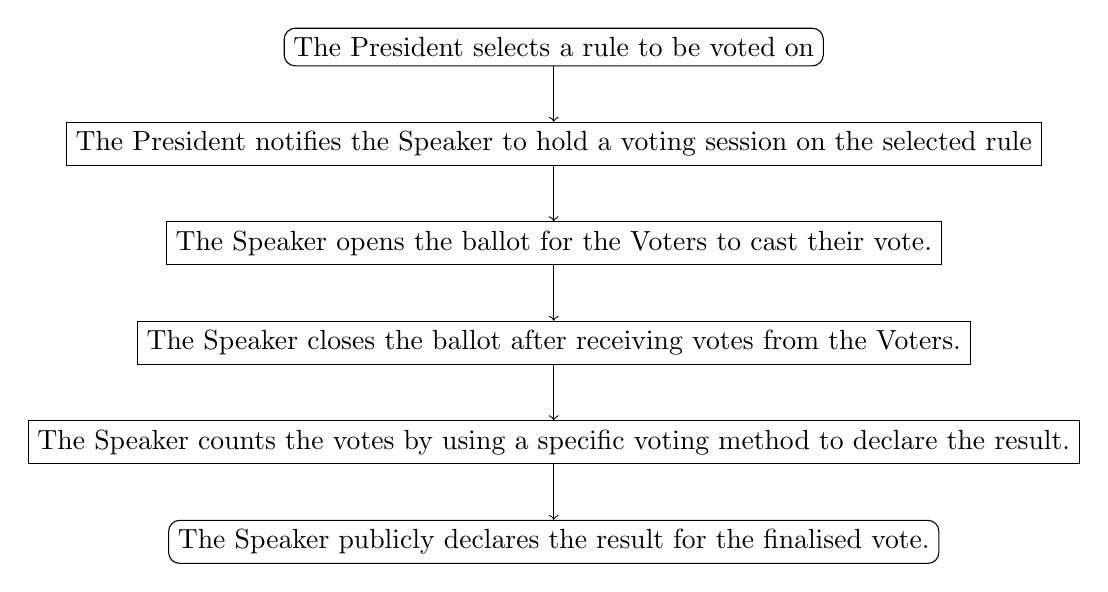
\begin{tikzpicture}[node distance=20pt]
\centering
\node[draw, rounded corners] (start)  {The President selects a rule to be voted on};
\node[draw, below=of start] (step 1)  {The President notifies the Speaker to hold a voting session on the selected rule};
\node[draw, below=of step 1] (step 2)  {The Speaker opens the ballot for the Voters to cast their vote.};
\node[draw, below=of step 2] (step 3)  {The Speaker closes the ballot after receiving votes from the Voters.};
\node[draw, below=of step 3] (step 4)  {The Speaker counts the votes by using a specific voting method to declare the result.};
\node[draw, below=of step 4, rounded corners] (end)   {The Speaker publicly declares the result for the finalised vote.};
 \draw[->] (start)  -- (step 1);
 \draw[->] (step 1) -- (step 2);
 \draw[->] (step 2) -- (step 3);
 \draw[->] (step 3) -- (step 4);
 \draw[->] (step 4) -- (end);
\end{tikzpicture}
\caption{Voting Protocol for Rules}
\label{fig:RONRVotingProtocol}
\end{center}
\end{figure}

For elections of roles, the sequence of actions of the voting protocol is mostly similar to the above explanation in principle, except for some parameters, such as the motion of the vote which is the role itself (President, or Speaker, or Judge), the facilitator of the election/vote event which depends on what role is being held for election (refer to Chapter 5 IIGO for more details on change of roles and power transfer), and the applicable voting method function to call for election that will produce the result, which is different from the voting method used for rules. Refer to Section~\ref{sec:VotingMethods} for more details on voting methods to be used for elections of roles.

At the start of the game, it is assumed that all 6 islands have the power to vote at any necessary voting scenario, and no diplomatic sanction is in place for any island. However, in the further turns of the game, some island(s) could lose their right to vote and/or not permitted to participate in a voting event due to the diplomatic sanction(s) in place. Refer to Chapter 5 IIGO for details on diplomatic sanction. In this case, the Speaker will open the ballots to the eligible islands only , i.e. those who are permitted to vote at a certain state of the game.

% Implmentaion section deleted

    \chapter{Team 1 Agent Design}

\section{Core Idea}
Team 1 agent was designed around the idea that the agent wants the whole archipelago to survive. However, the agent does have different configurations to allow for some malicious behaviour in order to facilitate some interesting agent interactions.

\section{Emotional state}

The agent's behaviour is affected by what we have termed her \emph{emotional state}. This is governed by the agent's current resources in relation to the living cost.

\begin{table} [htb]
    \centering
    \begin{tabular}{|l|l|}
        \hline
        \textbf{Emotional State} & \textbf{Condition} \\
        \hline
        Happy & Default state \\
        \hline
        Anxious & Current resources under 5 times the living costs \\
        \hline
        Desperate & Agent in critical state \\
        \hline
    \end{tabular}
\end{table}


\section{Opinions on Islands}
As information and resource sharing between islands is possible, it is possible and desirable for the agent to form an opinion of other islands. This be used to gauge the accuracy of information from other islands as well as, potentially, deny resource sharing to islands deemed ``selfish''.

Initially, opinion on all islands is neutral. Over time, through IITO and IIGO, opinions on islands will change. This will affect behaviour in IITO, as well as IIGO voting. Note that positive values correspond to positive opinions while negative values correspond to negative opinions.

\section{IITO Gifts}
When team 1 agent receives a request for gifts, the agent will decide how much to offer depending on the agent's current emotional state and the opinion of that island.

\begin{table} [htb]
    \centering
    \begin{tabular}{|c|p{0.5\textwidth}|}
        \hline
        \textbf{Emotional State} & \textbf{How is IITO handled?} \\
        \hline
        Happy & Agent will give away resources that satisfies the requested amount. Up to a percent of available resources. \\
        \hline
        Anxious & Agent will give away a ratio of the requested amount and its current resources. \\
        \hline
        Desperate & Agent will refuse any gift requests that it receives. \\
        \hline
    \end{tabular}
\end{table}

During IITO, the agent's opinion of other islands is affected. For every gift received, the agent's opinion of the gift-giver increases. However, the agent's opinion of an island can decrease if that island promised a gift and did not fulfil it.

Moreover, if the agent's opinion of an island is very high, the agent can decide to give gifts disregarding the agent's own anxiety. On the other hand, if an opinion of an island is very low, the agent can decide to refuse to send a gift even though the agent is happy.

For increase survivability, team 1 agent will accept any gift offers that it receives.

\subsection{Future Work}
Team 1 agent currently has a very straightforward IITO strategy. Possible alteration to this strategy could include:
\begin{itemize}
    \item Being less susceptible to bribery. The agent should stop increasing the opinion of an island after receiving $X$ amount of continuous gifts.
    \item Stop handing out gifts to islands that are not in critical state.
    \item Being proactive in bribery. The agent will give non-requested gifts to the current president in hopes that this will reduce tax and increase resource allocation from the common pool.
\end{itemize}

\section{IIFO Disaster Prediction}
Disasters can happen deterministically or stochastically (see Chapter~\ref{sec: Disaster} for more information). For an agent, it is important to predict when a disaster occurs so that as much disaster damage is mitigated using the common pool.

When the game starts, the disaster prediction made by the agent is random. This prediction always has a confidence value of $0$. As more disasters occur, a history of disasters is built up. Using this history, the mean disaster position ($x$, $y$), magnitude and period is calculated. A confidence value is calculated along with the mean disaster metrics and shared along with the prediction.

% Add a footnote on website?  https://www.mathsisfun.com/data/confidence-interval.html
The confidence value is calculated by finding the ratio between margin of error and the mean value. The smaller the margin of error, the more confident the agent is in her prediction. Therefore, a difference between the mean value and the margin of error must also be calculated. The confidence interval equation is used to calculate the margin of error:

\begin{equation}
    \label{eq: Team1MarginOfError}
    \textsc{Error} = Z \dfrac{s}{\sqrt{n}}
\end{equation}

where $s$, $n$ and $Z$ are the standard deviation, size of array and confidence interval respectively.

Using the difference between the mean value ($\bar{x}$) and the margin of error and taking the ratio of this result over the mean will provide the agent with the confidence value.
\begin{equation}
    \textsc{Confidence Value} = \frac{\bar{x} - \textsc{Error}}{\bar{x}}
\end{equation}.

The agent maintains a \textbf{trust score} for every island \emph{including itself}. This is based on the accuracy of islands' prediction of time left to the disaster.

Sharing and obtaining other disaster information to and from other islands respectively can increase the survivability of the archipelago. As more disaster predictions are shared, a network of trust between team 1 agent and other islands is built.

\subsection{Future Work}
While team 1 agent has a satisfactory disaster prediction algorithm, it does not make use of this prediction or predictions from other islands in any meaningful way. This is primarily due to disaster prediction being one of the last features to be implemented and not enough time being available to complete it.

Nevertheless, here are some possible uses for the disaster prediction system.

\begin{itemize}
  \item \textbf{Tax policy} --- As president, the agent could choose to increase or decrease taxation depending on (predicted) time left to disaster.
  \item \textbf{Voting} --- A trustworthy island could make for a better president, speaker or judge, as they would be able to act according to imminent disasters.
  \item \textbf{Common pool contribution} --- Based on predicted disaster location the agent may increase or decrease her common pool contribution. If a disaster is expected to affect the agent significantly then she could choose to mitigate resource loss by contributing a large amount to the common pool, as the alternative would be losing more resources.
\end{itemize}

Finally, prediction accuracy could be improved by using the prediction of the most trustworthy island, whether that is the agent herself or not, or averaging the predictions of the most trustworthy islands.

\section{IIGO: President}

Following the agent's core idea, as the president, the agent will try to enlarge the common pool as well as redistribute wealth among the islands, in an attempt to ensure the survival of as many islands as possible. This is achieved through an aggressive, tiered tax policy as well as denying common pool allocation requests to the wealthier islands.

This policy had to be verified as it could be vulnerable to ``free-rider'' islands, who could avoid paying tax and still reap the benefits of disaster protection from a large common pool and ``bailout'' allocations when they are low on resources.

As a test of this, a simulation was set up with a variable number of lawful and free-rider islands in order to measure the stability of this policy.

Three tax evading islands (half of the islands) was found to be the limit at which this policy would lead to collapse of the IIGO and the common pool. This was deemed an acceptable limit as at least half of the other agent teams would obey tax policy, at least most of the time or with a small amount of evasion. The resource graphs for the cases of two and three tax evading islands can be seen in \autoref{fig:team1:two_invaders} and \autoref{fig:team1:three_invaders}.

\begin{figure}[H]
\centering
\includegraphics[width=0.9\textwidth]{09_team1_agentdesign/images/two_invaders}
\caption{Resource graph. Islands 5 and 6 are evading tax.}
\label{fig:team1:two_invaders}
\end{figure}

\begin{figure}[H]
\centering
\includegraphics[width=0.9\textwidth]{09_team1_agentdesign/images/three_invaders}
\caption{Resource graph. Islands 4 to 6 are evading tax.}
\label{fig:team1:three_invaders}
\end{figure}

Note here that collapse of IIGO (as in \autoref{fig:team1:three_invaders}, with three tax evaders) does not automatically imply collapse of the archipelago; the islands appeared to survive (and, in fact, thrive) even after the collapse of IIGO.\@ It was taken as an assumption that this was only due to the uniformity of strategies, and in the ``real'' simulation, with heterogeneous agents, collapse of IIGO would lead to collapse of the archipelago.



\section{Foraging}
Multiple foraging strategies were developed, initially by intuition and later by attempting to address the shortcomings of previous attempts. They were developed in order and aptly named:
\begin{itemize}
    \item Return on Investment (ROI)
    \item Regression
    \item Flip Forage
\end{itemize}


\subsection{Return on Investment (ROI) Foraging}%
\label{sec:forage-roi}

This first algorithm is based on repeating successful foraging behaviours in the past, whether those be by the agent herself or another agent.

For the first few turns (the exact amount is configurable) the agent will forage randomly.

The agent maintains a history of foraging decisions and outcomes, including those received from IIFO.\@ When it comes time to forage, this history is sorted by ROI, i.e.\ the ratio of profit to contribution. Decisions that resulted in a loss, had profit smaller than the living cost, or had a larger contribution than a (configurable) percentage of available resources, are filtered out.

\subsection{Regression Foraging}%
\label{sec:forage-regression}

This strategy tries to predict the ideal foraging decision, even if that exact decision was not made in the past. This is done using regression, which is used to find the decision with the highest expected reward.

The \emph{regression} strategy forages randomly in the initial turns and history is kept as in \nameref{sec:forage-roi}. To make a foraging decision, the history is split by foraged resource (fish or deer), and quadratic regression is performed on contribution versus reward for both resources. From this, a quadratic equation is formed. If the quadratic equation found is negative then the optimal contribution can be found by differentiation. If it is positive then a (large) value is chosen as contribution, as a higher contribution should simply lead to a higher reward.

\subsection{Flip Foraging}

This strategy chooses the least foraged resource from the last turn, according to IIFO-reported data. Contributed amount is proportional to the chosen resource's total ROI from last turn. This choice was made under the assumption that ROI is an indicator of the resource's ``condition''. If a resource only gives moderate rewards (proportionally to input) it means that it is probably over-used currently and as such agents should allow it to recover, by scaling down their foraging attempts or by switching foraging types.

\subsection{Comparison}

To compare the three strategies, simulations were run with six agents, two using \emph{ROI foraging}, two using \emph{regression foraging}, and two using \emph{flip foraging}. IIGO and IITO were also disabled in order to isolate the efficacy of foraging methods from other parts of the game. The simulation was run five times and the results averaged over the 5 games as well as the two agents following the same strategy.

\begin{figure}[H] 
\centering
\includegraphics[width=0.6\textwidth]{09_team1_agentdesign/images/mean_survival_turns}
\caption{Mean survival turns for different strategies.}
\label{fig:team1:mean_survival}
\end{figure} 

\begin{figure}[H] 
\centering
\includegraphics[width=0.6\textwidth]{09_team1_agentdesign/images/total_efficiency}
\caption{Average foraging efficiency}
\label{fig:team1:average_efficiency}
\end{figure} 

It is clear from \autoref{fig:team1:mean_survival} that the \emph{flip} foraging strategy dominates the other two in terms of overall effectiveness. However, it is interesting to note that, according to \autoref{fig:team1:average_efficiency}, the \emph{ROI} foraging method is almost as efficient as \emph{flip}, which raises the question of what causes the difference in their success. This difference could be attributed to one core issue with the \emph{ROI strategy}: ignoring the absolute value of rewards. The agent will happily settle for a profit of $11$ resources, if that was obtained with a contribution of $0.1$ resources (a profit of $110000\%$) over a profit $50$ resources for a contribution of $25$ (a measly $100\%$). This means that in the long run living costs overwhelm the \emph{ROI} agent. The \emph{flip} agent does not take expected profit into account and as such is unaffected by this.

\emph{Regression} appears to occupy a medium between \emph{flip} and \emph{ROI}, however it is much less consistent, as evidenced by the error bars in \autoref{fig:team1:mean_survival}, with \emph{regression} surviving for under 10 turns in some runs.

%%% Local Variables:
%%% mode: latex
%%% TeX-master: "../main"
%%% End:

    \chapter{Inter-Island Governmental Organisation (IIGO)}


The role of IIGO is to maintain, update, and revise the rules concerning provision to managing the long-term collective risk dilemma (ltCRD). 

\begin{itemize}
    \item There will be 3 distinct branches in the IIGO: the \textbf{legislative branch}, \textbf{executive branch} and \textbf{judicial branch}\footnote{This is, as no surprise, inspired by the separation of powers in Western democracies.}.
    \item Each role is put in power according to the  transfer-of-power rules (see Section~\ref{subsec:transfer-of-power} for more detail).
    \item The head of the legislative branch is the Speaker, the head of the executive branch is the President, and the head of judicial branch is the Judge.
    \begin{itemize}
        \item  The Speaker, President and Judge are selected, through a democratic election, from the islands in the archipelago\footnote{This naming is inspired by the roles in the US Government.}.
        \item The resources gathered by the archipelago are endogenous, hence acting on the institutional powers granted to the Speaker, President or Judge costs resources. 
        \item For their duty, the President, the Speaker and the Judge receive a salary for each of their turns in office (see Section~\ref{subsec:salary} for more detail).
        \item The limit of the powers of the President, Speaker and Judge are defined in this chapter (e.g. the Speaker can only call one vote per turn).
 
    \end{itemize}
\end{itemize}

\subsection{IIGO Specific Definitions}
\begin{definition} \label{def:ballot}
    A \textbf{ballot} is related to each island's \textbf{power} to support or disagree with the rule specified in the vote called by the President and to vote in favour or against an island for a specific role (i.e. the President, Speaker, Judge) at each round of the game.
\end{definition}


%\begin{definition} \label{def:vote}
    %A \textbf{vote} is related to a role's (i.e. the President, Speaker, Judge) \textbf{power} to call a vote for a specific rule or an election.
%\end{definition}


\begin{definition} \label{def:tax}
    The \textbf{taxation} is related to the President's \textbf{power} to request a specific \underline{\textbf{minimum}} amount of contribution from each island to the common pool at each round of the game. 
\end{definition}

\begin{definition} \label{def:alloc_req}
    An \textbf{allocation request} is related to each island's \textbf{power} to request a specific amount of resource allocation from the President at each round of the game.
\end{definition}


\begin{definition} \label{def:rule_prop_list}
A \textbf{rule proposal list} is related to each island's \textbf{power} to propose a specific rule to be passed to the President at each round of the game.
\end{definition}

\begin{definition} \label{def:invst}
    An \textbf{investigation} is related to the Judge's \textbf{power} to acquire information to make a decision, followed by a calculation of the expected results and checking whether some specific rules have been obeyed, exclusively for the actions carried out by the \textbf{islands}. 
\end{definition}


An example of an \emph{investigation}: The President has permitted the island $X$ to take the amount of $Y$ resources from the common pool. Upon \emph{investigation} carried out by the Judge, it is revealed that the amount of resources taken out from the common pool by the island $X$ is, in fact, $Y'$ such that $Y' \neq Y$.


\begin{definition}
\textbf{Monitoring} is a government official's \textbf{power} to perform event recognition and to check whether some specific rules have been obeyed.
\end{definition}

An example of \emph{monitoring}: The Speaker has performed only the following action: \emph{counted the votes and calculated the result} for a rule. Upon \emph{monitoring} carried out by the President, it is noticed that the Speaker has not made any \emph{announcement}. Hence, the Speaker has not followed their obligation to \emph{announce} the result of any vote held.

See Section~\ref{sec:accountability} for more information about which roles can monitor which ones.


\begin{definition}
\textbf{Investigative-monitoring} is a government official's \textbf{power} to acquire the information used in acting on a governmental power followed by calculation of the expected results and checking whether some specific rules have been obeyed, exclusively for the actions carried out by a government official they are responsible for.
\end{definition}

An example of \emph{investigative-monitoring}: The Speaker has performed the following actions: \emph{counted the votes and calculated the result $R$} for a vote $V$ and \emph{announced} the result $R'$ for the vote $V$. Upon \emph{investigative-monitoring} carried out by the President, it is noticed that $R' \neq R$. Hence, the Speaker has modified the announced result.


\begin{definition}
The \textbf{sanction} is related to the Judge's \emph{power} to punish non-compliant islands when their disobedience is confirmed through investigations at a specific turn.
\end{definition}


\begin{definition}
The (judicial) \textbf{pardon} is related to the Judge's \emph{power} to forgive a non-compliant island at a specific turn.
\end{definition}

\begin{definition}
The \textbf{budget} is the maximum amount of resources a role is permitted to spend from the common pool as it performs its own institutional-power-enabled actions at a specific turn.
\end{definition}


\begin{definition}
The \textbf{salary} is the amount of resources a role is to be given from the common pool as a reward for performing its institutional-power-enabled actions at a specific turn.
\end{definition}

\begin{definition} \label{def:term}
A \textbf{term} is the number of turns an island is \emph{permitted} to hold a role, and after which the responsible role (indicated in the transfer-of-power cycle in Figure~\ref{fig:cycles_in_IIGO}) is \emph{obliged} to initiate transfer-of-power.
\end{definition}

\subsection{\emph{Power}, \emph{Permission} and \emph{Obligation} Distinction}
In the rest of the specifications, we will be specifically using the following three terms to define the actions and responsibilities carried out by the Speaker, President, Judge (see Figure~ \ref{fig:per_obl_sets}):
\begin{itemize}
    \item Power
    \item Permission
    \item Obligation
\end{itemize}



\begin{figure}[H] 
\centering
\includegraphics[width=0.6\textwidth]{05_iigo/images/SOMAS_per_obl.pdf}
\caption{Relationship between \emph{power}, \emph{permission} and \emph{obligation}.}
\label{fig:per_obl_sets}
\end{figure} 


For example, the Judge has the \emph{power} to carry out investigations at an IIGO session. There are no rules specifying which specific islands the Judge should investigate. Therefore, the Judge has the \emph{permission} to investigate any `alive' islands during a session. However, the Judge is \emph{obliged} to make at least some number of investigations each turn.



\section{Executive Branch}
\label{sec:executive}
The executive branch is responsible for \textbf{carrying out the law}.
\begin{itemize}
       
    \item The President has the \emph{power} to: 
    \begin{itemize}
        
        \item Select a rule for voting $R^{*}$ to be passed to the Speaker.
        \begin{rule_IIGO}
            The President has the \emph{obligation} to \emph{select} a rule $R^{*}$ if the \emph{rule proposal list} has at least one proposed rule in it.
        \end{rule_IIGO}
        \begin{rule_IIGO}
            The President has the \emph{permission} to \emph{select} a rule $R^{*}$ if and only if $R^{*} \in S$, where $S$ is the \emph{rule proposal list}.
        \end{rule_IIGO}
        
        \item Decide the amount of individual \emph{taxation} (i.e. a specific \emph{minimum} amount of contribution to the common pool for each island) for the current turn.
        
        \begin{itemize}
            \item The President is given the self-reported resource amounts held by each island to assist in this decision.
            %\item Suggested Rule: For any island that has chosen to not report it's resources, the President has the \emph{obligation} to set them an individual tax amount T.
        \end{itemize}
        
        \item Decide the allocation of resources distributed from the common pool to the islands (i.e. a specific \emph{maximum} amount an island is permitted to take from the common pool).
        
        \begin{itemize}
            \item The President is given the \emph{allocation requests} made by each island.
            %\item \emph{}{Suggested Rule:} The President has an obligation to prioritise islands in critical condition.
        \end{itemize}
    \end{itemize}
\end{itemize}



\section{Legislative Branch}
\label{sec:legislative}
The legislative branch is responsible for \textbf{making the law}.
\begin{itemize}

    \item The Speaker has the \emph{power} to:
    \begin{itemize}
        
        \item Call a vote $V$ for a rule $R$.
        \begin{rule_IIGO}
            The Speaker has the \emph{obligation} to \emph{call} a vote $V$ if and only if the President has \emph{selected} a rule $R$ to be voted on.
        \end {rule_IIGO}
        \begin{rule_IIGO}
            The Speaker has the \emph{permission} to \emph{call} a vote $V$ for a rule $R$ if and only if the rule $R = R^{*}$, where $R^{*}$ is the rule \emph{selected} by the President.
        \end {rule_IIGO}
            
        \item Choose which islands are participating in the vote $V$.
       % \footnote{This is our sequential implementation alternative for the power to close the ballot box.}.
        \begin{rule_IIGO}
            The Speaker has the \emph{obligation} to ask for a vote from all alive islands.
        \end {rule_IIGO}
            
        \item Declare the result $C$ of a vote $V$. 
        \begin{rule_IIGO}
            The Speaker has the \emph{obligation} to \emph{declare the result} $C$ for a vote $V$ if and only if the vote V has been \emph{called}.
        \end {rule_IIGO}
        \begin{rule_IIGO}
            The Speaker has the \emph{permission} to \emph{declare the result} $C$ for a vote $V$ if $C = C^{*}$, where $C^{*}$ is the result produced by \emph{calling} the vote $V$.
        \end {rule_IIGO}
        \begin{itemize}
            \item This step is what enables a rule to be \emph{active}.
        \end{itemize}
    \end{itemize}
\end{itemize}




\section{Judicial Branch}
\label{sec:judicial}

The judicial branch is responsible for \textbf{evaluating the law}.
\begin{itemize}
    \item The Judge has the \emph{power} to:
    \begin{itemize}
        \item Perform a number of \emph{inspections}\footnote{An \emph{inspection} \textbf{costs} an expense of resources (See Definition~\ref{def:invst} for more detail).} $I$ and produce a compliance outcome $\mathbb{O}^{*}$\footnote{Note that the compliance outcome $\mathbb{O}^{*}$ considered is a boolean.}.
        %(true: the island has been compliant with the rules in play, false: the island has not been compliant with the rules in play)
        %\begin{itemize}
           % \item For example, to check if the event outcome is \emph{concurrent}\footnote{Again, what is defined as "concurrent"? A clear definition is needed.} with the rules.
        %\end{itemize}
        \begin{rule_IIGO}
            The Judge has the \emph{obligation} to make at least $N$ investigations at each turn.
        \end{rule_IIGO}
        \item Declare the outcome $\mathbb{O}$ of an inspection $I$ to all islands\footnote{This act of broadcasting is especially important for islands to form an opinion about the sanctioned islands accordingly.}.
        \begin{rule_IIGO}
            The Judge has the \emph{obligation} to declare the outcome $\mathbb{O}$ of an inspection $I$ if and only if the inspection $I$ has been performed.
        \end{rule_IIGO}
        \begin{rule_IIGO}
            The Judge has the \emph{permission} to declare the outcome $\mathbb{O}$ of an inspection $I$ if $\mathbb{O} = \mathbb{O}^{*}$, where $\mathbb{O}^{*}$ is the outcome of the inspection $I$.
        \end{rule_IIGO}
        %\item Initiate the removal of the \texttt{President}.
        %\begin{itemize}
            %\item A good Judge would be especially vigilant during \emph{power transfer} regarding the \emph{President} position (see Section~\ref{leg_const} for more detail).
        %\end{itemize}
        \item Invoke economic \textbf{sanctions} (see Section~\ref{sec:sanctions} for more detail).
        \begin{rule_IIGO}
            The Judge has the \emph{obligation} to invoke a sanction $S$ for an island $X$ if and only if an investigation $I$ has an outcome $\mathbb{O}^{*}$ indicating non-compliance, and $I$ is an investigation of an action taken by island $X$.
        \end{rule_IIGO}
        \item Invoke even more severe sanctions in the case of further disobedience to previous sanction(s).
        \begin{rule_IIGO}
            The Judge has the \emph{permission} to invoke a severer sanction $S'$ for an island $X$ if the island $X$ has not fulfilled the requirements of the previous sanction $S$.
        \end{rule_IIGO}
        \item Pardon the islands which are currently sanctioned.
        \begin{rule_IIGO}
            The Judge has the \emph{permission} to revoke any sanction $S$ of an island $X$ at a specific turn.
        \end{rule_IIGO}
    \end{itemize}
\end{itemize}
%(e.g. a new rule that falls under a "sanction" category \hl{[I'm not sure about this being a `new rule` [Ezgi]]}

\subsection{Sanctions}
\label{sec:sanctions}
All sanctions are of economic nature which include:
        \begin{itemize}
            %\item Revoking an island's access to the common pool.
            \item Enforcing an island to contribute a specific amount of resources to the common pool.
            \begin{itemize}
                \item This does not mean that the Judge has the \emph{power} to take resources from an island in order to put them to the common pool -- the island itself is expected to carry out this implication imposed by the sanction itself, otherwise further punishment can be induced by the Judge.
                \item Similarly, \emph{opinion formulation} will follow accordingly whether the island(s) is/are following the implications imposed by the sanction(s).
            \end{itemize}
        
    \end{itemize}
    Sanctions are the associated penalty that comes with an island breaking a specific rule. The Judge is in full control of the penalties associated with breaking any rules. Once the Judge has specified the score of the penalty associated with each time an island breaks a rule, the cumulative penalties accumulated by the island are then used to determine which \textbf{sanction tier} that each island falls into. The score threshold to determine the boundaries of the sanction tiers are set by the Judge. At each turn of the game, each island is told whether they are being sanctioned, and if so, which \textbf{sanction tier} that they are currently in. The \textbf{sanction tiers} of the non-compliant islands are also broadcasted to the other islands in the archipelago. To summarise, the sanctioning process follows these steps:
    
    
    
    %Sanctions are based on an island breaking a rule. Each rule must therefore have an associated penalty. By default, we set these penalties such that they add $1$ to the total sanction score for each island. However, we allow the judge to override this scoring, the judge is able to set their own scores for any particular rule as they desire. This custom scoring is then used when an island breaks a particular rule. By looking at events that occurred in the last turn, and using the customised scoring we provide the holder of the judge role with full control of the penalties for breaking any rules.
    
    





%we then use the cumulative penalties accumulated by each island to determine which Sanction Tier they fall into. The score threshold's required to fall into these sanction tiers is set by the judge and is checked for monotonicity. Each island is told whether they are being sanctioned, and is so what tier they are in. We also tell other islands about which sanction tiers other islands have fallen into. 

    \begin{enumerate}
        \item The Judge has the \emph{power} to set custom penalties associated with breaking any rules.
        \item The Judge is given a list of all events that occurred in the previous turn.
        \item The Judge has the \emph{power} to check whether any, or all of these previous events, involve the islands in the archipelago breaking any rules.
        \item Each of the transgressions is scored using the Judge's custom penalties if the Judge has set them. Otherwise, a score of $1$ is given each time a rule is broken.
        \item The Judge has the \emph{power} to revise the sanction thresholds.
        \item Using the latest sanction thresholds available, each island is assigned to a sanction tier based on the sanction score that it has received.
        \item These sanction tiers are broadcasted to all of the islands in the archipelago.
        \item The Judge then uses sanctions rules in place to calculate the specific amount of resources that each non-compliant island has in order to determine how much it should contribute to the common pool, based on the sanction tier that it is in.
    \end{enumerate}



\section{Constitutional Rights and Obligations in the Archipelago}
\label{sec:const_rights_obl_archi}
Each island has the \emph{power} to:
\begin{itemize}
\item make an \emph{allocation request} (see Definition~\ref{def:alloc_req}) to the President for a specific amount to be allocated to them.
\item report the number of resources it is in possession of to the President.
\begin{rule_IIGO}
    Each island has the \emph{obligation} to report the number of resources it is in possession of to the President.
\end{rule_IIGO}
\begin{rule_IIGO}
    Each island has the \emph{permission} to report the number of resources $R'$ if and only if $R' = R$, where R is the number of resources the island is in possession of.
\end{rule_IIGO}
\item take resources from the common pool.


\begin{rule_IIGO}
    Each island has the \emph{permission} to take at maximum $N$ resources, where $N$ is the specific allocation made by the President to that island\footnote{If no such allocation is made, the island is \emph{permitted} to take any amount of resources.}.
\end{rule_IIGO}
\item contribute resources to the common pool.
\begin{rule_IIGO}
    Each island has the \emph{obligation} to contribute to the common pool an amount greater or equal to that of the individual tax set by the President.
\end{rule_IIGO}
                %The President is in
                %(unless there is a rule in place that dictates how Speaker is to allocate resources).
\item add a rule to the \emph{rule proposal list} (see Definition~\ref{def:rule_prop_list}) at the start of each turn.
        %\begin{itemize}
            %\item The game specification includes how many rules an island can propose each turn.
        %\end{itemize}
        %\item vote  for rules in the Legislative Branch and vote for their favourite islands in elections
\item participate in the legislative branch of the government by casting ballots in votes called by the Speaker
\item vote for an island to be elected for a specific role (e.g. the President, Judge, Speaker) during the elections\footnote{This will be assumed to be true \underline{unless stated otherwise}. %Note that \textbf{diplomatic sanctions} can disable this power of a specific island (see Section~\ref{jud_const}).}.
        }.
\end{itemize}
\section{Accountability Cycle}
\label{sec:accountability}


To ensure that the government avoids corruption and abuse of power, each branch is accountable to another. The President is accountable to the Speaker, the Speaker is accountable to the Judge, and the Judge is accountable to the President (see Figure~ \ref{fig:cycles_in_IIGO}). This accountability cycle is enacted through \emph{monitoring} actions\footnote{Note that the terms \textbf{monitoring} and \textbf{investigation} have similar but quite different meanings in the IIGO context.}. 

The powers related to the accountability cycle and transfer-of-power for each role can be summarized as the following: 
\begin{itemize}
    \item The Speaker has the \emph{power} to: 
    \begin{itemize}
        \item monitor the President.
        \item announce the result of this monitoring.
        \item initiate the transfer-of-power for the Judge.
    \end{itemize}
    \item The President has the \emph{power} to: 
    \begin{itemize}
        \item monitor the Judge.
        \item announce the result of this monitoring.
        \item initiate the transfer-of-power for the Speaker.
    \end{itemize}
    \item The Judge has the \emph{power} to: 
    \begin{itemize}
        \item  monitor the Speaker.
        \item announce the result of this monitoring.
        \item initiate the transfer-of-power for the President.
    \end{itemize}
\end{itemize}

%Unlike investigations performed by the Judge, who performs investigations on island actions in the following turn, each role is given the opportunity to check up on the actions of the role it is responsible for immediately after they have been performed. In this sense, the President can monitor (includes investigative-monitoring) the powers (calling a vote and announcing the result) acted on by the Speaker immediately after the Speaker's announcement (or lack there of). The government officials hold a lot of power so this is to ensure that any wrong-doing is determined as quickly as possible. For this project we are only pursuing one degree of monitoring, that is, the powers relating to the accountability cycle will not be monitored themselves. We assume that agents will act in the interest of themselves and keeping all the islands alive is beneficial to everyone. Hence, while the agents might be inclined to break rules in order to benefit themselves, anyone else breaking the rules is seen as undesirable under the assumption that the system in place is there to benefit all. 


Through the proposed accountability cycle, each role is given the opportunity to check up on the actions of the role it is accountable for immediately after they have been performed. It is clear that the IIGO roles (i.e. the President, Speaker and Judge) hold a considerable amount of \emph{power} in their hands. The accountability cycle is designed to address the possible abuses of this power. With monitoring, any wrong-doing in the IGO is determined as quickly as possible and the role in question can be replaced. 

Within the scope of the coursework, we decided to pursue only \emph{one degree of monitoring}, meaning that the powers relating to the accountability cycle will not be monitored themselves. We assume that agents will act in the interest of all the islands in the archipelago. Hence, while the agents might be inclined to break the rules to benefit in some form, it is assumed that the others will negatively see any non-compliant islands based on the assumption that the proposed IIGO system is in place to maintain the welfare of all the islands.

Let role $X$ be accountable to the role $Y$, which is accountable to the role $Z$. Then:
\begin{rule_IIGO}
$Y$ has the \emph{obligation} to declare the outcome of the monitoring result $M$ associated with the action $A$ undertaken by $X$ if and only if $Y$ has monitored the action $A$ performed by $X$. 
\end{rule_IIGO}
\begin{rule_IIGO}
$Y$ has the \emph{permission} to declare the monitoring result $M$ associated with the action $A$ undertaken by $X$ if and only if $M = M^{*}$, where $M^{*}$ is the outcome of \emph{monitoring} action $A$ performed by $X$\footnote{These constitutional rules should be available to the agents to check their decision against. However, due to having only one degree of accountability cycle in place, these rules are not enforced through any sanctions (i.e. breaking these rules has no consequences as they only deem to be an \emph{agreement} among the roles).}.
\end{rule_IIGO}


\begin{figure}[!htb]
\centering
\includegraphics[scale=0.33]{05_iigo/images/role cycles.png}
\caption{Accountability cycle (left), the transfer-of-power cycle (middle) and salary cycle (right).}
\label{fig:cycles_in_IIGO}
\end{figure}


\subsection{Transfer-of-power}
\label{subsec:transfer-of-power}
\begin{enumerate}
    \item The Speaker conducts a vote for the election of the new Judge.
    \item The Judge conducts a vote for the election of the new President.
    \item The President conducts a vote for the election of the new Speaker.
\end{enumerate}
Refer to the Figure~ \ref{fig:cycles_in_IIGO} for further clarification about the transfer-of-power cycle.

\begin{rule_IIGO}
   The role $X$ has the \emph{obligation} to conduct a vote for the election of $Y$ at the end of the term (see Definition~\ref{def:term}) if and only if the role $X$ is accountable to the role $Y$. 
\end{rule_IIGO}.

\section{Budget and Salary}
\subsection{Budget}
%Actions associated with the IIGO have an associated cost that is defined as a configuration parameter. The institutional-power-enabled actions of  identified to require a "computational" component are:

Institutional-enabled-power actions in the IIGO have an associated cost with them. Some examples for such actions include:


%that is defined as a configuration parameter. The institutional-power-enabled actions of  identified to require a "computational" component are:


%We have defined the resource to be an endogenous one, hence any computation surrounding the distribution of the resource must use up some of that resource. 
\begin{itemize}
\item Calling any vote and computing the winner.
\item Declaring (e.g. \textit{announcing} the result of a vote).
\item Setting the amount of \emph{taxation} for each island.
\item Deciding the allocation distribution for each island.
\item Inspecting an island's action history.
\item Monitoring a role.
\end{itemize}

Since IIGO has been designed to act in the common good, IIGO-related costs will be directly withdrawn from the common pool. Since the common pool is considered a communal property of the archipelago, there are rules in place to limit how much each role is allowed to spend in order to perform its own institutional-power-enabled actions. This is the reason why defining the \emph{budget} and keeping it separate for each of the three IIGO roles.


As a role performs institutional-enabled-power actions, the corresponding cost associated with this action is subtracted from the role's budget. A budget of zero means that the role does not have the \emph{power} to perform any of its institutional-power-enabled actions. The removal of the budget rule from the rules in play means the role is allowed to perform as many such actions as it prefers to (as long as those actions are not governed by other rules). 



%As a role performs an endogenous-cost action, the corresponding cost associated with this action is subtracted from the role's budget. Thus, if as a result of an endogenous-cost action a role will be left with negative budget, it will have gone over the budget limit and will have broken the budget rule. A budget of zero means that the role is not allowed to perform any of its institutional-power-enabled actions associated an endogenous-cost. The removal of the budget rule from the rules in play means the role is allowed to perform as many such actions as it pleases (as long as those actions are not governed by other rules). 

The budget rule is also persistent across turns. This means that, assuming nothing else affects the budget, if a role has $100$ resources in its budget at each turn and spends only $10$ resources, this means that this very same role has $90$ resources in its budget at the next turn. On the other hand, islands can choose to increase the budget periodically every turn. This is governed by another budget extension rule.




%one turn and it spends 10, it has 90 resources in it's budget the next turn. 

Finally, it must be noted that the budget is inherently linked with the fact that whether obligations of a specific role can be undergone.
For example, during \emph{monitoring}, it should not be seen as a rule violation if a role has not acted on an obligation if it would go over the budget as a result. 

%This can also be seen as an added clause "... and the action is only permitted if they have the budget" to most rules which govern actions with an endogenous-cost.
%\begin{rule_IIGO}
    %The budget is increased by an amount $N$ every turn.
%\end{rule_IIGO}

%This rule means that, assuming nothing else affects the budget, if a budget is set to increase by 10 resources every turn and the budget is a 100 resources in turn one, the budget is 110 resources in turn 2. Setting this rule to 0 is equal to removing this rule and it means that the budget is never increased. 


\subsection{Salary}
\label{subsec:salary}
A salary is paid to each role in power as an incentive to act in a publicly approved way. %Hence, each role has the \emph{power} to pay a salary to another role following the salary cycle in Figure~\ref{fig:cycles_in_IIGO}.
\begin{rule_IIGO} \label{rule:salary}
   %Each role has the \emph{obligation} to pay the salary of amount $S$ to another if and only if the amount paid $S'$ is equal to $S$.
   Each role has the \emph{obligation} to pay the salary of amount $S$ to one another following the salary cycle in Figure~\ref{fig:cycles_in_IIGO}.
\end{rule_IIGO}

In Rule~\ref{rule:salary}, setting $S=0$ (through changing the active rules in place) means that roles do not have the permission to pay any salary. Removing the Rule~\ref{rule:salary} means that the roles may freely choose the amount $S$ for the salary payments.

\section{IIGO Session order}

\begin{enumerate}
    \item The Judge has the \emph{power} to check the history of actions to confirm whether the previously punished island(s) has/have obeyed the previous round's sanctions, meaning whether they contributed to the common pool accordingly in case of economic sanctions.
    %\begin{itemize}
      %  \item \emph{Suggested Rule:} In case of disobeying sanctions, the Judge is \emph{obliged} and \emph{permitted} to increase the severity of sanctions with respect to specific islands.
   % \end{itemize}
    \item The Judge has the \emph{power} to carry out \emph{inspections} on the history of actions of any island $X$ to check whether:
        \begin{enumerate}
        \item the reported resources of $X$ in the previous round match the real value of resources $X$ had in its private pool for the previous turn.
        \item the island $X$ has retrieved the right amount of the resources from the common pool, based on the \emph{allocation request} evaluated by the previous President.
            \begin{itemize}
            \item An example: In the previous round, the President has decided that the island $X$ can take $Y$ amount of resources from the common pool. If the Judge finds out that the island $X$ has taken an amount of $Y'$ such that $Y' > Y$, the Judge has the \emph{power} to invoke sanctions on the island $X$.
            
            %the Judge is \emph{obliged} and \emph{permitted} to sanction island $X$.
            \end{itemize}
        \end{enumerate}
    \item The Judge has the \emph{power} to invoke sanctions based on the outcome of the inspections.
    \item The President has the \emph{power} to decide to carry out a \emph{monitoring} on:
        \begin{enumerate}
        \item the sanctions imposed by the Judge.
        \end{enumerate}
    \item The islands may report the resources in their private pools to the President.
    \item The President has the \emph{power} to let each island know about the amount of \emph{taxation} they have to pay.
    \item The island has the \emph{power} to make an \emph{allocation request} to the President.
    \item The President has the \emph{power} decide on an allocation of resources and let each island know about the amount of resource allocation they are permitted to take from the common pool.
    \item The island has the \emph{power} to pick and to propose a rule to be voted on to the President.
    \item The President has the \emph{power} to choose a rule to be voted on from the received rule proposals.
    \item The Speaker has the \emph{power} to decide to carry out a \emph{monitoring} on: 
        \begin{enumerate}
        \item the resource allocation decided by the President.
        \item the rule proposed by the President.
        \end{enumerate}
    \item The Speaker has the \emph{power} to call a vote.
        \begin{enumerate}
        \item The islands vote in support of, or against, the rule (aye or nay) anonymously.
        \end{enumerate}
    \item The Speaker has the \emph{power} to announce a result of a vote to the islands and carries out the law change, if required (e.g. deleting/rejecting a rule if there is a majority nay vote).
    \item The Judge has the \emph{power} to decide to carry out \emph{monitoring} on:
        \begin{enumerate}
        \item the vote called by the Speaker.
        \item the Speaker announcing the result.
    \end{enumerate}
    \item The roles pay salary for one another following the accountability cycle in Figure~ \ref{fig:cycles_in_IIGO}.

\end{enumerate}



\section{Future Work}

\begin{itemize}
    \item \textbf{Diplomatic sanctions}: Although having the potential of being a good alternative for severer sanctions discussed in  Section~\ref{sec:sanctions}, diplomatic sanctions are \emph{not} implemented within the scope of the coursework. \\
    Suggested diplomatic sanctions include:
        \begin{itemize}
            \item Revoking an island's eligibility to vote and to be elected for a position.
            \item Revoking an island's eligibility to propose a rule/motion.
        \end{itemize}
    \item \textbf{Immutable rules}: Within the scope of the coursework, a subset of rules could have been categorised as immutable. This means that to change such immutable rules, the islands first need to vote to change their status to be \emph{mutable}, and consequently, hold another vote to change these mutable rules.
    %\item \textbf{Adding rules to the proposal list: } 
\end{itemize}

    \chapter{Inter-Island Governmental Organisation (IIGO)}


The role of IIGO is to maintain, update, and revise the rules concerning provision to managing the long-term collective risk dilemma (ltCRD). 

\begin{itemize}
    \item There will be 3 distinct branches in the IIGO: the \textbf{legislative branch}, \textbf{executive branch} and \textbf{judicial branch}\footnote{This is, as no surprise, inspired by the separation of powers in Western democracies.}.
    \item Each role is put in power according to the  transfer-of-power rules (see Section~\ref{subsec:transfer-of-power} for more detail).
    \item The head of the legislative branch is the Speaker, the head of the executive branch is the President, and the head of judicial branch is the Judge.
    \begin{itemize}
        \item  The Speaker, President and Judge are selected, through a democratic election, from the islands in the archipelago\footnote{This naming is inspired by the roles in the US Government.}.
        \item The resources gathered by the archipelago are endogenous, hence acting on the institutional powers granted to the Speaker, President or Judge costs resources. 
        \item For their duty, the President, the Speaker and the Judge receive a salary for each of their turns in office (see Section~\ref{subsec:salary} for more detail).
        \item The limit of the powers of the President, Speaker and Judge are defined in this chapter (e.g. the Speaker can only call one vote per turn).
 
    \end{itemize}
\end{itemize}

\subsection{IIGO Specific Definitions}
\begin{definition} \label{def:ballot}
    A \textbf{ballot} is related to each island's \textbf{power} to support or disagree with the rule specified in the vote called by the President and to vote in favour or against an island for a specific role (i.e. the President, Speaker, Judge) at each round of the game.
\end{definition}


%\begin{definition} \label{def:vote}
    %A \textbf{vote} is related to a role's (i.e. the President, Speaker, Judge) \textbf{power} to call a vote for a specific rule or an election.
%\end{definition}


\begin{definition} \label{def:tax}
    The \textbf{taxation} is related to the President's \textbf{power} to request a specific \underline{\textbf{minimum}} amount of contribution from each island to the common pool at each round of the game. 
\end{definition}

\begin{definition} \label{def:alloc_req}
    An \textbf{allocation request} is related to each island's \textbf{power} to request a specific amount of resource allocation from the President at each round of the game.
\end{definition}


\begin{definition} \label{def:rule_prop_list}
A \textbf{rule proposal list} is related to each island's \textbf{power} to propose a specific rule to be passed to the President at each round of the game.
\end{definition}

\begin{definition} \label{def:invst}
    An \textbf{investigation} is related to the Judge's \textbf{power} to acquire information to make a decision, followed by a calculation of the expected results and checking whether some specific rules have been obeyed, exclusively for the actions carried out by the \textbf{islands}. 
\end{definition}


An example of an \emph{investigation}: The President has permitted the island $X$ to take the amount of $Y$ resources from the common pool. Upon \emph{investigation} carried out by the Judge, it is revealed that the amount of resources taken out from the common pool by the island $X$ is, in fact, $Y'$ such that $Y' \neq Y$.


\begin{definition}
\textbf{Monitoring} is a government official's \textbf{power} to perform event recognition and to check whether some specific rules have been obeyed.
\end{definition}

An example of \emph{monitoring}: The Speaker has performed only the following action: \emph{counted the votes and calculated the result} for a rule. Upon \emph{monitoring} carried out by the President, it is noticed that the Speaker has not made any \emph{announcement}. Hence, the Speaker has not followed their obligation to \emph{announce} the result of any vote held.

See Section~\ref{sec:accountability} for more information about which roles can monitor which ones.


\begin{definition}
\textbf{Investigative-monitoring} is a government official's \textbf{power} to acquire the information used in acting on a governmental power followed by calculation of the expected results and checking whether some specific rules have been obeyed, exclusively for the actions carried out by a government official they are responsible for.
\end{definition}

An example of \emph{investigative-monitoring}: The Speaker has performed the following actions: \emph{counted the votes and calculated the result $R$} for a vote $V$ and \emph{announced} the result $R'$ for the vote $V$. Upon \emph{investigative-monitoring} carried out by the President, it is noticed that $R' \neq R$. Hence, the Speaker has modified the announced result.


\begin{definition}
The \textbf{sanction} is related to the Judge's \emph{power} to punish non-compliant islands when their disobedience is confirmed through investigations at a specific turn.
\end{definition}


\begin{definition}
The (judicial) \textbf{pardon} is related to the Judge's \emph{power} to forgive a non-compliant island at a specific turn.
\end{definition}

\begin{definition}
The \textbf{budget} is the maximum amount of resources a role is permitted to spend from the common pool as it performs its own institutional-power-enabled actions at a specific turn.
\end{definition}


\begin{definition}
The \textbf{salary} is the amount of resources a role is to be given from the common pool as a reward for performing its institutional-power-enabled actions at a specific turn.
\end{definition}

\begin{definition} \label{def:term}
A \textbf{term} is the number of turns an island is \emph{permitted} to hold a role, and after which the responsible role (indicated in the transfer-of-power cycle in Figure~\ref{fig:cycles_in_IIGO}) is \emph{obliged} to initiate transfer-of-power.
\end{definition}

\subsection{\emph{Power}, \emph{Permission} and \emph{Obligation} Distinction}
In the rest of the specifications, we will be specifically using the following three terms to define the actions and responsibilities carried out by the Speaker, President, Judge (see Figure~ \ref{fig:per_obl_sets}):
\begin{itemize}
    \item Power
    \item Permission
    \item Obligation
\end{itemize}



\begin{figure}[H] 
\centering
\includegraphics[width=0.6\textwidth]{05_iigo/images/SOMAS_per_obl.pdf}
\caption{Relationship between \emph{power}, \emph{permission} and \emph{obligation}.}
\label{fig:per_obl_sets}
\end{figure} 


For example, the Judge has the \emph{power} to carry out investigations at an IIGO session. There are no rules specifying which specific islands the Judge should investigate. Therefore, the Judge has the \emph{permission} to investigate any `alive' islands during a session. However, the Judge is \emph{obliged} to make at least some number of investigations each turn.



\section{Executive Branch}
\label{sec:executive}
The executive branch is responsible for \textbf{carrying out the law}.
\begin{itemize}
       
    \item The President has the \emph{power} to: 
    \begin{itemize}
        
        \item Select a rule for voting $R^{*}$ to be passed to the Speaker.
        \begin{rule_IIGO}
            The President has the \emph{obligation} to \emph{select} a rule $R^{*}$ if the \emph{rule proposal list} has at least one proposed rule in it.
        \end{rule_IIGO}
        \begin{rule_IIGO}
            The President has the \emph{permission} to \emph{select} a rule $R^{*}$ if and only if $R^{*} \in S$, where $S$ is the \emph{rule proposal list}.
        \end{rule_IIGO}
        
        \item Decide the amount of individual \emph{taxation} (i.e. a specific \emph{minimum} amount of contribution to the common pool for each island) for the current turn.
        
        \begin{itemize}
            \item The President is given the self-reported resource amounts held by each island to assist in this decision.
            %\item Suggested Rule: For any island that has chosen to not report it's resources, the President has the \emph{obligation} to set them an individual tax amount T.
        \end{itemize}
        
        \item Decide the allocation of resources distributed from the common pool to the islands (i.e. a specific \emph{maximum} amount an island is permitted to take from the common pool).
        
        \begin{itemize}
            \item The President is given the \emph{allocation requests} made by each island.
            %\item \emph{}{Suggested Rule:} The President has an obligation to prioritise islands in critical condition.
        \end{itemize}
    \end{itemize}
\end{itemize}



\section{Legislative Branch}
\label{sec:legislative}
The legislative branch is responsible for \textbf{making the law}.
\begin{itemize}

    \item The Speaker has the \emph{power} to:
    \begin{itemize}
        
        \item Call a vote $V$ for a rule $R$.
        \begin{rule_IIGO}
            The Speaker has the \emph{obligation} to \emph{call} a vote $V$ if and only if the President has \emph{selected} a rule $R$ to be voted on.
        \end {rule_IIGO}
        \begin{rule_IIGO}
            The Speaker has the \emph{permission} to \emph{call} a vote $V$ for a rule $R$ if and only if the rule $R = R^{*}$, where $R^{*}$ is the rule \emph{selected} by the President.
        \end {rule_IIGO}
            
        \item Choose which islands are participating in the vote $V$.
       % \footnote{This is our sequential implementation alternative for the power to close the ballot box.}.
        \begin{rule_IIGO}
            The Speaker has the \emph{obligation} to ask for a vote from all alive islands.
        \end {rule_IIGO}
            
        \item Declare the result $C$ of a vote $V$. 
        \begin{rule_IIGO}
            The Speaker has the \emph{obligation} to \emph{declare the result} $C$ for a vote $V$ if and only if the vote V has been \emph{called}.
        \end {rule_IIGO}
        \begin{rule_IIGO}
            The Speaker has the \emph{permission} to \emph{declare the result} $C$ for a vote $V$ if $C = C^{*}$, where $C^{*}$ is the result produced by \emph{calling} the vote $V$.
        \end {rule_IIGO}
        \begin{itemize}
            \item This step is what enables a rule to be \emph{active}.
        \end{itemize}
    \end{itemize}
\end{itemize}




\section{Judicial Branch}
\label{sec:judicial}

The judicial branch is responsible for \textbf{evaluating the law}.
\begin{itemize}
    \item The Judge has the \emph{power} to:
    \begin{itemize}
        \item Perform a number of \emph{inspections}\footnote{An \emph{inspection} \textbf{costs} an expense of resources (See Definition~\ref{def:invst} for more detail).} $I$ and produce a compliance outcome $\mathbb{O}^{*}$\footnote{Note that the compliance outcome $\mathbb{O}^{*}$ considered is a boolean.}.
        %(true: the island has been compliant with the rules in play, false: the island has not been compliant with the rules in play)
        %\begin{itemize}
           % \item For example, to check if the event outcome is \emph{concurrent}\footnote{Again, what is defined as "concurrent"? A clear definition is needed.} with the rules.
        %\end{itemize}
        \begin{rule_IIGO}
            The Judge has the \emph{obligation} to make at least $N$ investigations at each turn.
        \end{rule_IIGO}
        \item Declare the outcome $\mathbb{O}$ of an inspection $I$ to all islands\footnote{This act of broadcasting is especially important for islands to form an opinion about the sanctioned islands accordingly.}.
        \begin{rule_IIGO}
            The Judge has the \emph{obligation} to declare the outcome $\mathbb{O}$ of an inspection $I$ if and only if the inspection $I$ has been performed.
        \end{rule_IIGO}
        \begin{rule_IIGO}
            The Judge has the \emph{permission} to declare the outcome $\mathbb{O}$ of an inspection $I$ if $\mathbb{O} = \mathbb{O}^{*}$, where $\mathbb{O}^{*}$ is the outcome of the inspection $I$.
        \end{rule_IIGO}
        %\item Initiate the removal of the \texttt{President}.
        %\begin{itemize}
            %\item A good Judge would be especially vigilant during \emph{power transfer} regarding the \emph{President} position (see Section~\ref{leg_const} for more detail).
        %\end{itemize}
        \item Invoke economic \textbf{sanctions} (see Section~\ref{sec:sanctions} for more detail).
        \begin{rule_IIGO}
            The Judge has the \emph{obligation} to invoke a sanction $S$ for an island $X$ if and only if an investigation $I$ has an outcome $\mathbb{O}^{*}$ indicating non-compliance, and $I$ is an investigation of an action taken by island $X$.
        \end{rule_IIGO}
        \item Invoke even more severe sanctions in the case of further disobedience to previous sanction(s).
        \begin{rule_IIGO}
            The Judge has the \emph{permission} to invoke a severer sanction $S'$ for an island $X$ if the island $X$ has not fulfilled the requirements of the previous sanction $S$.
        \end{rule_IIGO}
        \item Pardon the islands which are currently sanctioned.
        \begin{rule_IIGO}
            The Judge has the \emph{permission} to revoke any sanction $S$ of an island $X$ at a specific turn.
        \end{rule_IIGO}
    \end{itemize}
\end{itemize}
%(e.g. a new rule that falls under a "sanction" category \hl{[I'm not sure about this being a `new rule` [Ezgi]]}

\subsection{Sanctions}
\label{sec:sanctions}
All sanctions are of economic nature which include:
        \begin{itemize}
            %\item Revoking an island's access to the common pool.
            \item Enforcing an island to contribute a specific amount of resources to the common pool.
            \begin{itemize}
                \item This does not mean that the Judge has the \emph{power} to take resources from an island in order to put them to the common pool -- the island itself is expected to carry out this implication imposed by the sanction itself, otherwise further punishment can be induced by the Judge.
                \item Similarly, \emph{opinion formulation} will follow accordingly whether the island(s) is/are following the implications imposed by the sanction(s).
            \end{itemize}
        
    \end{itemize}
    Sanctions are the associated penalty that comes with an island breaking a specific rule. The Judge is in full control of the penalties associated with breaking any rules. Once the Judge has specified the score of the penalty associated with each time an island breaks a rule, the cumulative penalties accumulated by the island are then used to determine which \textbf{sanction tier} that each island falls into. The score threshold to determine the boundaries of the sanction tiers are set by the Judge. At each turn of the game, each island is told whether they are being sanctioned, and if so, which \textbf{sanction tier} that they are currently in. The \textbf{sanction tiers} of the non-compliant islands are also broadcasted to the other islands in the archipelago. To summarise, the sanctioning process follows these steps:
    
    
    
    %Sanctions are based on an island breaking a rule. Each rule must therefore have an associated penalty. By default, we set these penalties such that they add $1$ to the total sanction score for each island. However, we allow the judge to override this scoring, the judge is able to set their own scores for any particular rule as they desire. This custom scoring is then used when an island breaks a particular rule. By looking at events that occurred in the last turn, and using the customised scoring we provide the holder of the judge role with full control of the penalties for breaking any rules.
    
    





%we then use the cumulative penalties accumulated by each island to determine which Sanction Tier they fall into. The score threshold's required to fall into these sanction tiers is set by the judge and is checked for monotonicity. Each island is told whether they are being sanctioned, and is so what tier they are in. We also tell other islands about which sanction tiers other islands have fallen into. 

    \begin{enumerate}
        \item The Judge has the \emph{power} to set custom penalties associated with breaking any rules.
        \item The Judge is given a list of all events that occurred in the previous turn.
        \item The Judge has the \emph{power} to check whether any, or all of these previous events, involve the islands in the archipelago breaking any rules.
        \item Each of the transgressions is scored using the Judge's custom penalties if the Judge has set them. Otherwise, a score of $1$ is given each time a rule is broken.
        \item The Judge has the \emph{power} to revise the sanction thresholds.
        \item Using the latest sanction thresholds available, each island is assigned to a sanction tier based on the sanction score that it has received.
        \item These sanction tiers are broadcasted to all of the islands in the archipelago.
        \item The Judge then uses sanctions rules in place to calculate the specific amount of resources that each non-compliant island has in order to determine how much it should contribute to the common pool, based on the sanction tier that it is in.
    \end{enumerate}



\section{Constitutional Rights and Obligations in the Archipelago}
\label{sec:const_rights_obl_archi}
Each island has the \emph{power} to:
\begin{itemize}
\item make an \emph{allocation request} (see Definition~\ref{def:alloc_req}) to the President for a specific amount to be allocated to them.
\item report the number of resources it is in possession of to the President.
\begin{rule_IIGO}
    Each island has the \emph{obligation} to report the number of resources it is in possession of to the President.
\end{rule_IIGO}
\begin{rule_IIGO}
    Each island has the \emph{permission} to report the number of resources $R'$ if and only if $R' = R$, where R is the number of resources the island is in possession of.
\end{rule_IIGO}
\item take resources from the common pool.


\begin{rule_IIGO}
    Each island has the \emph{permission} to take at maximum $N$ resources, where $N$ is the specific allocation made by the President to that island\footnote{If no such allocation is made, the island is \emph{permitted} to take any amount of resources.}.
\end{rule_IIGO}
\item contribute resources to the common pool.
\begin{rule_IIGO}
    Each island has the \emph{obligation} to contribute to the common pool an amount greater or equal to that of the individual tax set by the President.
\end{rule_IIGO}
                %The President is in
                %(unless there is a rule in place that dictates how Speaker is to allocate resources).
\item add a rule to the \emph{rule proposal list} (see Definition~\ref{def:rule_prop_list}) at the start of each turn.
        %\begin{itemize}
            %\item The game specification includes how many rules an island can propose each turn.
        %\end{itemize}
        %\item vote  for rules in the Legislative Branch and vote for their favourite islands in elections
\item participate in the legislative branch of the government by casting ballots in votes called by the Speaker
\item vote for an island to be elected for a specific role (e.g. the President, Judge, Speaker) during the elections\footnote{This will be assumed to be true \underline{unless stated otherwise}. %Note that \textbf{diplomatic sanctions} can disable this power of a specific island (see Section~\ref{jud_const}).}.
        }.
\end{itemize}
\section{Accountability Cycle}
\label{sec:accountability}


To ensure that the government avoids corruption and abuse of power, each branch is accountable to another. The President is accountable to the Speaker, the Speaker is accountable to the Judge, and the Judge is accountable to the President (see Figure~ \ref{fig:cycles_in_IIGO}). This accountability cycle is enacted through \emph{monitoring} actions\footnote{Note that the terms \textbf{monitoring} and \textbf{investigation} have similar but quite different meanings in the IIGO context.}. 

The powers related to the accountability cycle and transfer-of-power for each role can be summarized as the following: 
\begin{itemize}
    \item The Speaker has the \emph{power} to: 
    \begin{itemize}
        \item monitor the President.
        \item announce the result of this monitoring.
        \item initiate the transfer-of-power for the Judge.
    \end{itemize}
    \item The President has the \emph{power} to: 
    \begin{itemize}
        \item monitor the Judge.
        \item announce the result of this monitoring.
        \item initiate the transfer-of-power for the Speaker.
    \end{itemize}
    \item The Judge has the \emph{power} to: 
    \begin{itemize}
        \item  monitor the Speaker.
        \item announce the result of this monitoring.
        \item initiate the transfer-of-power for the President.
    \end{itemize}
\end{itemize}

%Unlike investigations performed by the Judge, who performs investigations on island actions in the following turn, each role is given the opportunity to check up on the actions of the role it is responsible for immediately after they have been performed. In this sense, the President can monitor (includes investigative-monitoring) the powers (calling a vote and announcing the result) acted on by the Speaker immediately after the Speaker's announcement (or lack there of). The government officials hold a lot of power so this is to ensure that any wrong-doing is determined as quickly as possible. For this project we are only pursuing one degree of monitoring, that is, the powers relating to the accountability cycle will not be monitored themselves. We assume that agents will act in the interest of themselves and keeping all the islands alive is beneficial to everyone. Hence, while the agents might be inclined to break rules in order to benefit themselves, anyone else breaking the rules is seen as undesirable under the assumption that the system in place is there to benefit all. 


Through the proposed accountability cycle, each role is given the opportunity to check up on the actions of the role it is accountable for immediately after they have been performed. It is clear that the IIGO roles (i.e. the President, Speaker and Judge) hold a considerable amount of \emph{power} in their hands. The accountability cycle is designed to address the possible abuses of this power. With monitoring, any wrong-doing in the IGO is determined as quickly as possible and the role in question can be replaced. 

Within the scope of the coursework, we decided to pursue only \emph{one degree of monitoring}, meaning that the powers relating to the accountability cycle will not be monitored themselves. We assume that agents will act in the interest of all the islands in the archipelago. Hence, while the agents might be inclined to break the rules to benefit in some form, it is assumed that the others will negatively see any non-compliant islands based on the assumption that the proposed IIGO system is in place to maintain the welfare of all the islands.

Let role $X$ be accountable to the role $Y$, which is accountable to the role $Z$. Then:
\begin{rule_IIGO}
$Y$ has the \emph{obligation} to declare the outcome of the monitoring result $M$ associated with the action $A$ undertaken by $X$ if and only if $Y$ has monitored the action $A$ performed by $X$. 
\end{rule_IIGO}
\begin{rule_IIGO}
$Y$ has the \emph{permission} to declare the monitoring result $M$ associated with the action $A$ undertaken by $X$ if and only if $M = M^{*}$, where $M^{*}$ is the outcome of \emph{monitoring} action $A$ performed by $X$\footnote{These constitutional rules should be available to the agents to check their decision against. However, due to having only one degree of accountability cycle in place, these rules are not enforced through any sanctions (i.e. breaking these rules has no consequences as they only deem to be an \emph{agreement} among the roles).}.
\end{rule_IIGO}


\begin{figure}[!htb]
\centering
\includegraphics[scale=0.33]{05_iigo/images/role cycles.png}
\caption{Accountability cycle (left), the transfer-of-power cycle (middle) and salary cycle (right).}
\label{fig:cycles_in_IIGO}
\end{figure}


\subsection{Transfer-of-power}
\label{subsec:transfer-of-power}
\begin{enumerate}
    \item The Speaker conducts a vote for the election of the new Judge.
    \item The Judge conducts a vote for the election of the new President.
    \item The President conducts a vote for the election of the new Speaker.
\end{enumerate}
Refer to the Figure~ \ref{fig:cycles_in_IIGO} for further clarification about the transfer-of-power cycle.

\begin{rule_IIGO}
   The role $X$ has the \emph{obligation} to conduct a vote for the election of $Y$ at the end of the term (see Definition~\ref{def:term}) if and only if the role $X$ is accountable to the role $Y$. 
\end{rule_IIGO}.

\section{Budget and Salary}
\subsection{Budget}
%Actions associated with the IIGO have an associated cost that is defined as a configuration parameter. The institutional-power-enabled actions of  identified to require a "computational" component are:

Institutional-enabled-power actions in the IIGO have an associated cost with them. Some examples for such actions include:


%that is defined as a configuration parameter. The institutional-power-enabled actions of  identified to require a "computational" component are:


%We have defined the resource to be an endogenous one, hence any computation surrounding the distribution of the resource must use up some of that resource. 
\begin{itemize}
\item Calling any vote and computing the winner.
\item Declaring (e.g. \textit{announcing} the result of a vote).
\item Setting the amount of \emph{taxation} for each island.
\item Deciding the allocation distribution for each island.
\item Inspecting an island's action history.
\item Monitoring a role.
\end{itemize}

Since IIGO has been designed to act in the common good, IIGO-related costs will be directly withdrawn from the common pool. Since the common pool is considered a communal property of the archipelago, there are rules in place to limit how much each role is allowed to spend in order to perform its own institutional-power-enabled actions. This is the reason why defining the \emph{budget} and keeping it separate for each of the three IIGO roles.


As a role performs institutional-enabled-power actions, the corresponding cost associated with this action is subtracted from the role's budget. A budget of zero means that the role does not have the \emph{power} to perform any of its institutional-power-enabled actions. The removal of the budget rule from the rules in play means the role is allowed to perform as many such actions as it prefers to (as long as those actions are not governed by other rules). 



%As a role performs an endogenous-cost action, the corresponding cost associated with this action is subtracted from the role's budget. Thus, if as a result of an endogenous-cost action a role will be left with negative budget, it will have gone over the budget limit and will have broken the budget rule. A budget of zero means that the role is not allowed to perform any of its institutional-power-enabled actions associated an endogenous-cost. The removal of the budget rule from the rules in play means the role is allowed to perform as many such actions as it pleases (as long as those actions are not governed by other rules). 

The budget rule is also persistent across turns. This means that, assuming nothing else affects the budget, if a role has $100$ resources in its budget at each turn and spends only $10$ resources, this means that this very same role has $90$ resources in its budget at the next turn. On the other hand, islands can choose to increase the budget periodically every turn. This is governed by another budget extension rule.




%one turn and it spends 10, it has 90 resources in it's budget the next turn. 

Finally, it must be noted that the budget is inherently linked with the fact that whether obligations of a specific role can be undergone.
For example, during \emph{monitoring}, it should not be seen as a rule violation if a role has not acted on an obligation if it would go over the budget as a result. 

%This can also be seen as an added clause "... and the action is only permitted if they have the budget" to most rules which govern actions with an endogenous-cost.
%\begin{rule_IIGO}
    %The budget is increased by an amount $N$ every turn.
%\end{rule_IIGO}

%This rule means that, assuming nothing else affects the budget, if a budget is set to increase by 10 resources every turn and the budget is a 100 resources in turn one, the budget is 110 resources in turn 2. Setting this rule to 0 is equal to removing this rule and it means that the budget is never increased. 


\subsection{Salary}
\label{subsec:salary}
A salary is paid to each role in power as an incentive to act in a publicly approved way. %Hence, each role has the \emph{power} to pay a salary to another role following the salary cycle in Figure~\ref{fig:cycles_in_IIGO}.
\begin{rule_IIGO} \label{rule:salary}
   %Each role has the \emph{obligation} to pay the salary of amount $S$ to another if and only if the amount paid $S'$ is equal to $S$.
   Each role has the \emph{obligation} to pay the salary of amount $S$ to one another following the salary cycle in Figure~\ref{fig:cycles_in_IIGO}.
\end{rule_IIGO}

In Rule~\ref{rule:salary}, setting $S=0$ (through changing the active rules in place) means that roles do not have the permission to pay any salary. Removing the Rule~\ref{rule:salary} means that the roles may freely choose the amount $S$ for the salary payments.

\section{IIGO Session order}

\begin{enumerate}
    \item The Judge has the \emph{power} to check the history of actions to confirm whether the previously punished island(s) has/have obeyed the previous round's sanctions, meaning whether they contributed to the common pool accordingly in case of economic sanctions.
    %\begin{itemize}
      %  \item \emph{Suggested Rule:} In case of disobeying sanctions, the Judge is \emph{obliged} and \emph{permitted} to increase the severity of sanctions with respect to specific islands.
   % \end{itemize}
    \item The Judge has the \emph{power} to carry out \emph{inspections} on the history of actions of any island $X$ to check whether:
        \begin{enumerate}
        \item the reported resources of $X$ in the previous round match the real value of resources $X$ had in its private pool for the previous turn.
        \item the island $X$ has retrieved the right amount of the resources from the common pool, based on the \emph{allocation request} evaluated by the previous President.
            \begin{itemize}
            \item An example: In the previous round, the President has decided that the island $X$ can take $Y$ amount of resources from the common pool. If the Judge finds out that the island $X$ has taken an amount of $Y'$ such that $Y' > Y$, the Judge has the \emph{power} to invoke sanctions on the island $X$.
            
            %the Judge is \emph{obliged} and \emph{permitted} to sanction island $X$.
            \end{itemize}
        \end{enumerate}
    \item The Judge has the \emph{power} to invoke sanctions based on the outcome of the inspections.
    \item The President has the \emph{power} to decide to carry out a \emph{monitoring} on:
        \begin{enumerate}
        \item the sanctions imposed by the Judge.
        \end{enumerate}
    \item The islands may report the resources in their private pools to the President.
    \item The President has the \emph{power} to let each island know about the amount of \emph{taxation} they have to pay.
    \item The island has the \emph{power} to make an \emph{allocation request} to the President.
    \item The President has the \emph{power} decide on an allocation of resources and let each island know about the amount of resource allocation they are permitted to take from the common pool.
    \item The island has the \emph{power} to pick and to propose a rule to be voted on to the President.
    \item The President has the \emph{power} to choose a rule to be voted on from the received rule proposals.
    \item The Speaker has the \emph{power} to decide to carry out a \emph{monitoring} on: 
        \begin{enumerate}
        \item the resource allocation decided by the President.
        \item the rule proposed by the President.
        \end{enumerate}
    \item The Speaker has the \emph{power} to call a vote.
        \begin{enumerate}
        \item The islands vote in support of, or against, the rule (aye or nay) anonymously.
        \end{enumerate}
    \item The Speaker has the \emph{power} to announce a result of a vote to the islands and carries out the law change, if required (e.g. deleting/rejecting a rule if there is a majority nay vote).
    \item The Judge has the \emph{power} to decide to carry out \emph{monitoring} on:
        \begin{enumerate}
        \item the vote called by the Speaker.
        \item the Speaker announcing the result.
    \end{enumerate}
    \item The roles pay salary for one another following the accountability cycle in Figure~ \ref{fig:cycles_in_IIGO}.

\end{enumerate}



\section{Future Work}

\begin{itemize}
    \item \textbf{Diplomatic sanctions}: Although having the potential of being a good alternative for severer sanctions discussed in  Section~\ref{sec:sanctions}, diplomatic sanctions are \emph{not} implemented within the scope of the coursework. \\
    Suggested diplomatic sanctions include:
        \begin{itemize}
            \item Revoking an island's eligibility to vote and to be elected for a position.
            \item Revoking an island's eligibility to propose a rule/motion.
        \end{itemize}
    \item \textbf{Immutable rules}: Within the scope of the coursework, a subset of rules could have been categorised as immutable. This means that to change such immutable rules, the islands first need to vote to change their status to be \emph{mutable}, and consequently, hold another vote to change these mutable rules.
    %\item \textbf{Adding rules to the proposal list: } 
\end{itemize}

    \chapter{Inter-Island Governmental Organisation (IIGO)}


The role of IIGO is to maintain, update, and revise the rules concerning provision to managing the long-term collective risk dilemma (ltCRD). 

\begin{itemize}
    \item There will be 3 distinct branches in the IIGO: the \textbf{legislative branch}, \textbf{executive branch} and \textbf{judicial branch}\footnote{This is, as no surprise, inspired by the separation of powers in Western democracies.}.
    \item Each role is put in power according to the  transfer-of-power rules (see Section~\ref{subsec:transfer-of-power} for more detail).
    \item The head of the legislative branch is the Speaker, the head of the executive branch is the President, and the head of judicial branch is the Judge.
    \begin{itemize}
        \item  The Speaker, President and Judge are selected, through a democratic election, from the islands in the archipelago\footnote{This naming is inspired by the roles in the US Government.}.
        \item The resources gathered by the archipelago are endogenous, hence acting on the institutional powers granted to the Speaker, President or Judge costs resources. 
        \item For their duty, the President, the Speaker and the Judge receive a salary for each of their turns in office (see Section~\ref{subsec:salary} for more detail).
        \item The limit of the powers of the President, Speaker and Judge are defined in this chapter (e.g. the Speaker can only call one vote per turn).
 
    \end{itemize}
\end{itemize}

\subsection{IIGO Specific Definitions}
\begin{definition} \label{def:ballot}
    A \textbf{ballot} is related to each island's \textbf{power} to support or disagree with the rule specified in the vote called by the President and to vote in favour or against an island for a specific role (i.e. the President, Speaker, Judge) at each round of the game.
\end{definition}


%\begin{definition} \label{def:vote}
    %A \textbf{vote} is related to a role's (i.e. the President, Speaker, Judge) \textbf{power} to call a vote for a specific rule or an election.
%\end{definition}


\begin{definition} \label{def:tax}
    The \textbf{taxation} is related to the President's \textbf{power} to request a specific \underline{\textbf{minimum}} amount of contribution from each island to the common pool at each round of the game. 
\end{definition}

\begin{definition} \label{def:alloc_req}
    An \textbf{allocation request} is related to each island's \textbf{power} to request a specific amount of resource allocation from the President at each round of the game.
\end{definition}


\begin{definition} \label{def:rule_prop_list}
A \textbf{rule proposal list} is related to each island's \textbf{power} to propose a specific rule to be passed to the President at each round of the game.
\end{definition}

\begin{definition} \label{def:invst}
    An \textbf{investigation} is related to the Judge's \textbf{power} to acquire information to make a decision, followed by a calculation of the expected results and checking whether some specific rules have been obeyed, exclusively for the actions carried out by the \textbf{islands}. 
\end{definition}


An example of an \emph{investigation}: The President has permitted the island $X$ to take the amount of $Y$ resources from the common pool. Upon \emph{investigation} carried out by the Judge, it is revealed that the amount of resources taken out from the common pool by the island $X$ is, in fact, $Y'$ such that $Y' \neq Y$.


\begin{definition}
\textbf{Monitoring} is a government official's \textbf{power} to perform event recognition and to check whether some specific rules have been obeyed.
\end{definition}

An example of \emph{monitoring}: The Speaker has performed only the following action: \emph{counted the votes and calculated the result} for a rule. Upon \emph{monitoring} carried out by the President, it is noticed that the Speaker has not made any \emph{announcement}. Hence, the Speaker has not followed their obligation to \emph{announce} the result of any vote held.

See Section~\ref{sec:accountability} for more information about which roles can monitor which ones.


\begin{definition}
\textbf{Investigative-monitoring} is a government official's \textbf{power} to acquire the information used in acting on a governmental power followed by calculation of the expected results and checking whether some specific rules have been obeyed, exclusively for the actions carried out by a government official they are responsible for.
\end{definition}

An example of \emph{investigative-monitoring}: The Speaker has performed the following actions: \emph{counted the votes and calculated the result $R$} for a vote $V$ and \emph{announced} the result $R'$ for the vote $V$. Upon \emph{investigative-monitoring} carried out by the President, it is noticed that $R' \neq R$. Hence, the Speaker has modified the announced result.


\begin{definition}
The \textbf{sanction} is related to the Judge's \emph{power} to punish non-compliant islands when their disobedience is confirmed through investigations at a specific turn.
\end{definition}


\begin{definition}
The (judicial) \textbf{pardon} is related to the Judge's \emph{power} to forgive a non-compliant island at a specific turn.
\end{definition}

\begin{definition}
The \textbf{budget} is the maximum amount of resources a role is permitted to spend from the common pool as it performs its own institutional-power-enabled actions at a specific turn.
\end{definition}


\begin{definition}
The \textbf{salary} is the amount of resources a role is to be given from the common pool as a reward for performing its institutional-power-enabled actions at a specific turn.
\end{definition}

\begin{definition} \label{def:term}
A \textbf{term} is the number of turns an island is \emph{permitted} to hold a role, and after which the responsible role (indicated in the transfer-of-power cycle in Figure~\ref{fig:cycles_in_IIGO}) is \emph{obliged} to initiate transfer-of-power.
\end{definition}

\subsection{\emph{Power}, \emph{Permission} and \emph{Obligation} Distinction}
In the rest of the specifications, we will be specifically using the following three terms to define the actions and responsibilities carried out by the Speaker, President, Judge (see Figure~ \ref{fig:per_obl_sets}):
\begin{itemize}
    \item Power
    \item Permission
    \item Obligation
\end{itemize}



\begin{figure}[H] 
\centering
\includegraphics[width=0.6\textwidth]{05_iigo/images/SOMAS_per_obl.pdf}
\caption{Relationship between \emph{power}, \emph{permission} and \emph{obligation}.}
\label{fig:per_obl_sets}
\end{figure} 


For example, the Judge has the \emph{power} to carry out investigations at an IIGO session. There are no rules specifying which specific islands the Judge should investigate. Therefore, the Judge has the \emph{permission} to investigate any `alive' islands during a session. However, the Judge is \emph{obliged} to make at least some number of investigations each turn.



\section{Executive Branch}
\label{sec:executive}
The executive branch is responsible for \textbf{carrying out the law}.
\begin{itemize}
       
    \item The President has the \emph{power} to: 
    \begin{itemize}
        
        \item Select a rule for voting $R^{*}$ to be passed to the Speaker.
        \begin{rule_IIGO}
            The President has the \emph{obligation} to \emph{select} a rule $R^{*}$ if the \emph{rule proposal list} has at least one proposed rule in it.
        \end{rule_IIGO}
        \begin{rule_IIGO}
            The President has the \emph{permission} to \emph{select} a rule $R^{*}$ if and only if $R^{*} \in S$, where $S$ is the \emph{rule proposal list}.
        \end{rule_IIGO}
        
        \item Decide the amount of individual \emph{taxation} (i.e. a specific \emph{minimum} amount of contribution to the common pool for each island) for the current turn.
        
        \begin{itemize}
            \item The President is given the self-reported resource amounts held by each island to assist in this decision.
            %\item Suggested Rule: For any island that has chosen to not report it's resources, the President has the \emph{obligation} to set them an individual tax amount T.
        \end{itemize}
        
        \item Decide the allocation of resources distributed from the common pool to the islands (i.e. a specific \emph{maximum} amount an island is permitted to take from the common pool).
        
        \begin{itemize}
            \item The President is given the \emph{allocation requests} made by each island.
            %\item \emph{}{Suggested Rule:} The President has an obligation to prioritise islands in critical condition.
        \end{itemize}
    \end{itemize}
\end{itemize}



\section{Legislative Branch}
\label{sec:legislative}
The legislative branch is responsible for \textbf{making the law}.
\begin{itemize}

    \item The Speaker has the \emph{power} to:
    \begin{itemize}
        
        \item Call a vote $V$ for a rule $R$.
        \begin{rule_IIGO}
            The Speaker has the \emph{obligation} to \emph{call} a vote $V$ if and only if the President has \emph{selected} a rule $R$ to be voted on.
        \end {rule_IIGO}
        \begin{rule_IIGO}
            The Speaker has the \emph{permission} to \emph{call} a vote $V$ for a rule $R$ if and only if the rule $R = R^{*}$, where $R^{*}$ is the rule \emph{selected} by the President.
        \end {rule_IIGO}
            
        \item Choose which islands are participating in the vote $V$.
       % \footnote{This is our sequential implementation alternative for the power to close the ballot box.}.
        \begin{rule_IIGO}
            The Speaker has the \emph{obligation} to ask for a vote from all alive islands.
        \end {rule_IIGO}
            
        \item Declare the result $C$ of a vote $V$. 
        \begin{rule_IIGO}
            The Speaker has the \emph{obligation} to \emph{declare the result} $C$ for a vote $V$ if and only if the vote V has been \emph{called}.
        \end {rule_IIGO}
        \begin{rule_IIGO}
            The Speaker has the \emph{permission} to \emph{declare the result} $C$ for a vote $V$ if $C = C^{*}$, where $C^{*}$ is the result produced by \emph{calling} the vote $V$.
        \end {rule_IIGO}
        \begin{itemize}
            \item This step is what enables a rule to be \emph{active}.
        \end{itemize}
    \end{itemize}
\end{itemize}




\section{Judicial Branch}
\label{sec:judicial}

The judicial branch is responsible for \textbf{evaluating the law}.
\begin{itemize}
    \item The Judge has the \emph{power} to:
    \begin{itemize}
        \item Perform a number of \emph{inspections}\footnote{An \emph{inspection} \textbf{costs} an expense of resources (See Definition~\ref{def:invst} for more detail).} $I$ and produce a compliance outcome $\mathbb{O}^{*}$\footnote{Note that the compliance outcome $\mathbb{O}^{*}$ considered is a boolean.}.
        %(true: the island has been compliant with the rules in play, false: the island has not been compliant with the rules in play)
        %\begin{itemize}
           % \item For example, to check if the event outcome is \emph{concurrent}\footnote{Again, what is defined as "concurrent"? A clear definition is needed.} with the rules.
        %\end{itemize}
        \begin{rule_IIGO}
            The Judge has the \emph{obligation} to make at least $N$ investigations at each turn.
        \end{rule_IIGO}
        \item Declare the outcome $\mathbb{O}$ of an inspection $I$ to all islands\footnote{This act of broadcasting is especially important for islands to form an opinion about the sanctioned islands accordingly.}.
        \begin{rule_IIGO}
            The Judge has the \emph{obligation} to declare the outcome $\mathbb{O}$ of an inspection $I$ if and only if the inspection $I$ has been performed.
        \end{rule_IIGO}
        \begin{rule_IIGO}
            The Judge has the \emph{permission} to declare the outcome $\mathbb{O}$ of an inspection $I$ if $\mathbb{O} = \mathbb{O}^{*}$, where $\mathbb{O}^{*}$ is the outcome of the inspection $I$.
        \end{rule_IIGO}
        %\item Initiate the removal of the \texttt{President}.
        %\begin{itemize}
            %\item A good Judge would be especially vigilant during \emph{power transfer} regarding the \emph{President} position (see Section~\ref{leg_const} for more detail).
        %\end{itemize}
        \item Invoke economic \textbf{sanctions} (see Section~\ref{sec:sanctions} for more detail).
        \begin{rule_IIGO}
            The Judge has the \emph{obligation} to invoke a sanction $S$ for an island $X$ if and only if an investigation $I$ has an outcome $\mathbb{O}^{*}$ indicating non-compliance, and $I$ is an investigation of an action taken by island $X$.
        \end{rule_IIGO}
        \item Invoke even more severe sanctions in the case of further disobedience to previous sanction(s).
        \begin{rule_IIGO}
            The Judge has the \emph{permission} to invoke a severer sanction $S'$ for an island $X$ if the island $X$ has not fulfilled the requirements of the previous sanction $S$.
        \end{rule_IIGO}
        \item Pardon the islands which are currently sanctioned.
        \begin{rule_IIGO}
            The Judge has the \emph{permission} to revoke any sanction $S$ of an island $X$ at a specific turn.
        \end{rule_IIGO}
    \end{itemize}
\end{itemize}
%(e.g. a new rule that falls under a "sanction" category \hl{[I'm not sure about this being a `new rule` [Ezgi]]}

\subsection{Sanctions}
\label{sec:sanctions}
All sanctions are of economic nature which include:
        \begin{itemize}
            %\item Revoking an island's access to the common pool.
            \item Enforcing an island to contribute a specific amount of resources to the common pool.
            \begin{itemize}
                \item This does not mean that the Judge has the \emph{power} to take resources from an island in order to put them to the common pool -- the island itself is expected to carry out this implication imposed by the sanction itself, otherwise further punishment can be induced by the Judge.
                \item Similarly, \emph{opinion formulation} will follow accordingly whether the island(s) is/are following the implications imposed by the sanction(s).
            \end{itemize}
        
    \end{itemize}
    Sanctions are the associated penalty that comes with an island breaking a specific rule. The Judge is in full control of the penalties associated with breaking any rules. Once the Judge has specified the score of the penalty associated with each time an island breaks a rule, the cumulative penalties accumulated by the island are then used to determine which \textbf{sanction tier} that each island falls into. The score threshold to determine the boundaries of the sanction tiers are set by the Judge. At each turn of the game, each island is told whether they are being sanctioned, and if so, which \textbf{sanction tier} that they are currently in. The \textbf{sanction tiers} of the non-compliant islands are also broadcasted to the other islands in the archipelago. To summarise, the sanctioning process follows these steps:
    
    
    
    %Sanctions are based on an island breaking a rule. Each rule must therefore have an associated penalty. By default, we set these penalties such that they add $1$ to the total sanction score for each island. However, we allow the judge to override this scoring, the judge is able to set their own scores for any particular rule as they desire. This custom scoring is then used when an island breaks a particular rule. By looking at events that occurred in the last turn, and using the customised scoring we provide the holder of the judge role with full control of the penalties for breaking any rules.
    
    





%we then use the cumulative penalties accumulated by each island to determine which Sanction Tier they fall into. The score threshold's required to fall into these sanction tiers is set by the judge and is checked for monotonicity. Each island is told whether they are being sanctioned, and is so what tier they are in. We also tell other islands about which sanction tiers other islands have fallen into. 

    \begin{enumerate}
        \item The Judge has the \emph{power} to set custom penalties associated with breaking any rules.
        \item The Judge is given a list of all events that occurred in the previous turn.
        \item The Judge has the \emph{power} to check whether any, or all of these previous events, involve the islands in the archipelago breaking any rules.
        \item Each of the transgressions is scored using the Judge's custom penalties if the Judge has set them. Otherwise, a score of $1$ is given each time a rule is broken.
        \item The Judge has the \emph{power} to revise the sanction thresholds.
        \item Using the latest sanction thresholds available, each island is assigned to a sanction tier based on the sanction score that it has received.
        \item These sanction tiers are broadcasted to all of the islands in the archipelago.
        \item The Judge then uses sanctions rules in place to calculate the specific amount of resources that each non-compliant island has in order to determine how much it should contribute to the common pool, based on the sanction tier that it is in.
    \end{enumerate}



\section{Constitutional Rights and Obligations in the Archipelago}
\label{sec:const_rights_obl_archi}
Each island has the \emph{power} to:
\begin{itemize}
\item make an \emph{allocation request} (see Definition~\ref{def:alloc_req}) to the President for a specific amount to be allocated to them.
\item report the number of resources it is in possession of to the President.
\begin{rule_IIGO}
    Each island has the \emph{obligation} to report the number of resources it is in possession of to the President.
\end{rule_IIGO}
\begin{rule_IIGO}
    Each island has the \emph{permission} to report the number of resources $R'$ if and only if $R' = R$, where R is the number of resources the island is in possession of.
\end{rule_IIGO}
\item take resources from the common pool.


\begin{rule_IIGO}
    Each island has the \emph{permission} to take at maximum $N$ resources, where $N$ is the specific allocation made by the President to that island\footnote{If no such allocation is made, the island is \emph{permitted} to take any amount of resources.}.
\end{rule_IIGO}
\item contribute resources to the common pool.
\begin{rule_IIGO}
    Each island has the \emph{obligation} to contribute to the common pool an amount greater or equal to that of the individual tax set by the President.
\end{rule_IIGO}
                %The President is in
                %(unless there is a rule in place that dictates how Speaker is to allocate resources).
\item add a rule to the \emph{rule proposal list} (see Definition~\ref{def:rule_prop_list}) at the start of each turn.
        %\begin{itemize}
            %\item The game specification includes how many rules an island can propose each turn.
        %\end{itemize}
        %\item vote  for rules in the Legislative Branch and vote for their favourite islands in elections
\item participate in the legislative branch of the government by casting ballots in votes called by the Speaker
\item vote for an island to be elected for a specific role (e.g. the President, Judge, Speaker) during the elections\footnote{This will be assumed to be true \underline{unless stated otherwise}. %Note that \textbf{diplomatic sanctions} can disable this power of a specific island (see Section~\ref{jud_const}).}.
        }.
\end{itemize}
\section{Accountability Cycle}
\label{sec:accountability}


To ensure that the government avoids corruption and abuse of power, each branch is accountable to another. The President is accountable to the Speaker, the Speaker is accountable to the Judge, and the Judge is accountable to the President (see Figure~ \ref{fig:cycles_in_IIGO}). This accountability cycle is enacted through \emph{monitoring} actions\footnote{Note that the terms \textbf{monitoring} and \textbf{investigation} have similar but quite different meanings in the IIGO context.}. 

The powers related to the accountability cycle and transfer-of-power for each role can be summarized as the following: 
\begin{itemize}
    \item The Speaker has the \emph{power} to: 
    \begin{itemize}
        \item monitor the President.
        \item announce the result of this monitoring.
        \item initiate the transfer-of-power for the Judge.
    \end{itemize}
    \item The President has the \emph{power} to: 
    \begin{itemize}
        \item monitor the Judge.
        \item announce the result of this monitoring.
        \item initiate the transfer-of-power for the Speaker.
    \end{itemize}
    \item The Judge has the \emph{power} to: 
    \begin{itemize}
        \item  monitor the Speaker.
        \item announce the result of this monitoring.
        \item initiate the transfer-of-power for the President.
    \end{itemize}
\end{itemize}

%Unlike investigations performed by the Judge, who performs investigations on island actions in the following turn, each role is given the opportunity to check up on the actions of the role it is responsible for immediately after they have been performed. In this sense, the President can monitor (includes investigative-monitoring) the powers (calling a vote and announcing the result) acted on by the Speaker immediately after the Speaker's announcement (or lack there of). The government officials hold a lot of power so this is to ensure that any wrong-doing is determined as quickly as possible. For this project we are only pursuing one degree of monitoring, that is, the powers relating to the accountability cycle will not be monitored themselves. We assume that agents will act in the interest of themselves and keeping all the islands alive is beneficial to everyone. Hence, while the agents might be inclined to break rules in order to benefit themselves, anyone else breaking the rules is seen as undesirable under the assumption that the system in place is there to benefit all. 


Through the proposed accountability cycle, each role is given the opportunity to check up on the actions of the role it is accountable for immediately after they have been performed. It is clear that the IIGO roles (i.e. the President, Speaker and Judge) hold a considerable amount of \emph{power} in their hands. The accountability cycle is designed to address the possible abuses of this power. With monitoring, any wrong-doing in the IGO is determined as quickly as possible and the role in question can be replaced. 

Within the scope of the coursework, we decided to pursue only \emph{one degree of monitoring}, meaning that the powers relating to the accountability cycle will not be monitored themselves. We assume that agents will act in the interest of all the islands in the archipelago. Hence, while the agents might be inclined to break the rules to benefit in some form, it is assumed that the others will negatively see any non-compliant islands based on the assumption that the proposed IIGO system is in place to maintain the welfare of all the islands.

Let role $X$ be accountable to the role $Y$, which is accountable to the role $Z$. Then:
\begin{rule_IIGO}
$Y$ has the \emph{obligation} to declare the outcome of the monitoring result $M$ associated with the action $A$ undertaken by $X$ if and only if $Y$ has monitored the action $A$ performed by $X$. 
\end{rule_IIGO}
\begin{rule_IIGO}
$Y$ has the \emph{permission} to declare the monitoring result $M$ associated with the action $A$ undertaken by $X$ if and only if $M = M^{*}$, where $M^{*}$ is the outcome of \emph{monitoring} action $A$ performed by $X$\footnote{These constitutional rules should be available to the agents to check their decision against. However, due to having only one degree of accountability cycle in place, these rules are not enforced through any sanctions (i.e. breaking these rules has no consequences as they only deem to be an \emph{agreement} among the roles).}.
\end{rule_IIGO}


\begin{figure}[!htb]
\centering
\includegraphics[scale=0.33]{05_iigo/images/role cycles.png}
\caption{Accountability cycle (left), the transfer-of-power cycle (middle) and salary cycle (right).}
\label{fig:cycles_in_IIGO}
\end{figure}


\subsection{Transfer-of-power}
\label{subsec:transfer-of-power}
\begin{enumerate}
    \item The Speaker conducts a vote for the election of the new Judge.
    \item The Judge conducts a vote for the election of the new President.
    \item The President conducts a vote for the election of the new Speaker.
\end{enumerate}
Refer to the Figure~ \ref{fig:cycles_in_IIGO} for further clarification about the transfer-of-power cycle.

\begin{rule_IIGO}
   The role $X$ has the \emph{obligation} to conduct a vote for the election of $Y$ at the end of the term (see Definition~\ref{def:term}) if and only if the role $X$ is accountable to the role $Y$. 
\end{rule_IIGO}.

\section{Budget and Salary}
\subsection{Budget}
%Actions associated with the IIGO have an associated cost that is defined as a configuration parameter. The institutional-power-enabled actions of  identified to require a "computational" component are:

Institutional-enabled-power actions in the IIGO have an associated cost with them. Some examples for such actions include:


%that is defined as a configuration parameter. The institutional-power-enabled actions of  identified to require a "computational" component are:


%We have defined the resource to be an endogenous one, hence any computation surrounding the distribution of the resource must use up some of that resource. 
\begin{itemize}
\item Calling any vote and computing the winner.
\item Declaring (e.g. \textit{announcing} the result of a vote).
\item Setting the amount of \emph{taxation} for each island.
\item Deciding the allocation distribution for each island.
\item Inspecting an island's action history.
\item Monitoring a role.
\end{itemize}

Since IIGO has been designed to act in the common good, IIGO-related costs will be directly withdrawn from the common pool. Since the common pool is considered a communal property of the archipelago, there are rules in place to limit how much each role is allowed to spend in order to perform its own institutional-power-enabled actions. This is the reason why defining the \emph{budget} and keeping it separate for each of the three IIGO roles.


As a role performs institutional-enabled-power actions, the corresponding cost associated with this action is subtracted from the role's budget. A budget of zero means that the role does not have the \emph{power} to perform any of its institutional-power-enabled actions. The removal of the budget rule from the rules in play means the role is allowed to perform as many such actions as it prefers to (as long as those actions are not governed by other rules). 



%As a role performs an endogenous-cost action, the corresponding cost associated with this action is subtracted from the role's budget. Thus, if as a result of an endogenous-cost action a role will be left with negative budget, it will have gone over the budget limit and will have broken the budget rule. A budget of zero means that the role is not allowed to perform any of its institutional-power-enabled actions associated an endogenous-cost. The removal of the budget rule from the rules in play means the role is allowed to perform as many such actions as it pleases (as long as those actions are not governed by other rules). 

The budget rule is also persistent across turns. This means that, assuming nothing else affects the budget, if a role has $100$ resources in its budget at each turn and spends only $10$ resources, this means that this very same role has $90$ resources in its budget at the next turn. On the other hand, islands can choose to increase the budget periodically every turn. This is governed by another budget extension rule.




%one turn and it spends 10, it has 90 resources in it's budget the next turn. 

Finally, it must be noted that the budget is inherently linked with the fact that whether obligations of a specific role can be undergone.
For example, during \emph{monitoring}, it should not be seen as a rule violation if a role has not acted on an obligation if it would go over the budget as a result. 

%This can also be seen as an added clause "... and the action is only permitted if they have the budget" to most rules which govern actions with an endogenous-cost.
%\begin{rule_IIGO}
    %The budget is increased by an amount $N$ every turn.
%\end{rule_IIGO}

%This rule means that, assuming nothing else affects the budget, if a budget is set to increase by 10 resources every turn and the budget is a 100 resources in turn one, the budget is 110 resources in turn 2. Setting this rule to 0 is equal to removing this rule and it means that the budget is never increased. 


\subsection{Salary}
\label{subsec:salary}
A salary is paid to each role in power as an incentive to act in a publicly approved way. %Hence, each role has the \emph{power} to pay a salary to another role following the salary cycle in Figure~\ref{fig:cycles_in_IIGO}.
\begin{rule_IIGO} \label{rule:salary}
   %Each role has the \emph{obligation} to pay the salary of amount $S$ to another if and only if the amount paid $S'$ is equal to $S$.
   Each role has the \emph{obligation} to pay the salary of amount $S$ to one another following the salary cycle in Figure~\ref{fig:cycles_in_IIGO}.
\end{rule_IIGO}

In Rule~\ref{rule:salary}, setting $S=0$ (through changing the active rules in place) means that roles do not have the permission to pay any salary. Removing the Rule~\ref{rule:salary} means that the roles may freely choose the amount $S$ for the salary payments.

\section{IIGO Session order}

\begin{enumerate}
    \item The Judge has the \emph{power} to check the history of actions to confirm whether the previously punished island(s) has/have obeyed the previous round's sanctions, meaning whether they contributed to the common pool accordingly in case of economic sanctions.
    %\begin{itemize}
      %  \item \emph{Suggested Rule:} In case of disobeying sanctions, the Judge is \emph{obliged} and \emph{permitted} to increase the severity of sanctions with respect to specific islands.
   % \end{itemize}
    \item The Judge has the \emph{power} to carry out \emph{inspections} on the history of actions of any island $X$ to check whether:
        \begin{enumerate}
        \item the reported resources of $X$ in the previous round match the real value of resources $X$ had in its private pool for the previous turn.
        \item the island $X$ has retrieved the right amount of the resources from the common pool, based on the \emph{allocation request} evaluated by the previous President.
            \begin{itemize}
            \item An example: In the previous round, the President has decided that the island $X$ can take $Y$ amount of resources from the common pool. If the Judge finds out that the island $X$ has taken an amount of $Y'$ such that $Y' > Y$, the Judge has the \emph{power} to invoke sanctions on the island $X$.
            
            %the Judge is \emph{obliged} and \emph{permitted} to sanction island $X$.
            \end{itemize}
        \end{enumerate}
    \item The Judge has the \emph{power} to invoke sanctions based on the outcome of the inspections.
    \item The President has the \emph{power} to decide to carry out a \emph{monitoring} on:
        \begin{enumerate}
        \item the sanctions imposed by the Judge.
        \end{enumerate}
    \item The islands may report the resources in their private pools to the President.
    \item The President has the \emph{power} to let each island know about the amount of \emph{taxation} they have to pay.
    \item The island has the \emph{power} to make an \emph{allocation request} to the President.
    \item The President has the \emph{power} decide on an allocation of resources and let each island know about the amount of resource allocation they are permitted to take from the common pool.
    \item The island has the \emph{power} to pick and to propose a rule to be voted on to the President.
    \item The President has the \emph{power} to choose a rule to be voted on from the received rule proposals.
    \item The Speaker has the \emph{power} to decide to carry out a \emph{monitoring} on: 
        \begin{enumerate}
        \item the resource allocation decided by the President.
        \item the rule proposed by the President.
        \end{enumerate}
    \item The Speaker has the \emph{power} to call a vote.
        \begin{enumerate}
        \item The islands vote in support of, or against, the rule (aye or nay) anonymously.
        \end{enumerate}
    \item The Speaker has the \emph{power} to announce a result of a vote to the islands and carries out the law change, if required (e.g. deleting/rejecting a rule if there is a majority nay vote).
    \item The Judge has the \emph{power} to decide to carry out \emph{monitoring} on:
        \begin{enumerate}
        \item the vote called by the Speaker.
        \item the Speaker announcing the result.
    \end{enumerate}
    \item The roles pay salary for one another following the accountability cycle in Figure~ \ref{fig:cycles_in_IIGO}.

\end{enumerate}



\section{Future Work}

\begin{itemize}
    \item \textbf{Diplomatic sanctions}: Although having the potential of being a good alternative for severer sanctions discussed in  Section~\ref{sec:sanctions}, diplomatic sanctions are \emph{not} implemented within the scope of the coursework. \\
    Suggested diplomatic sanctions include:
        \begin{itemize}
            \item Revoking an island's eligibility to vote and to be elected for a position.
            \item Revoking an island's eligibility to propose a rule/motion.
        \end{itemize}
    \item \textbf{Immutable rules}: Within the scope of the coursework, a subset of rules could have been categorised as immutable. This means that to change such immutable rules, the islands first need to vote to change their status to be \emph{mutable}, and consequently, hold another vote to change these mutable rules.
    %\item \textbf{Adding rules to the proposal list: } 
\end{itemize}

    \chapter{Inter-Island Governmental Organisation (IIGO)}


The role of IIGO is to maintain, update, and revise the rules concerning provision to managing the long-term collective risk dilemma (ltCRD). 

\begin{itemize}
    \item There will be 3 distinct branches in the IIGO: the \textbf{legislative branch}, \textbf{executive branch} and \textbf{judicial branch}\footnote{This is, as no surprise, inspired by the separation of powers in Western democracies.}.
    \item Each role is put in power according to the  transfer-of-power rules (see Section~\ref{subsec:transfer-of-power} for more detail).
    \item The head of the legislative branch is the Speaker, the head of the executive branch is the President, and the head of judicial branch is the Judge.
    \begin{itemize}
        \item  The Speaker, President and Judge are selected, through a democratic election, from the islands in the archipelago\footnote{This naming is inspired by the roles in the US Government.}.
        \item The resources gathered by the archipelago are endogenous, hence acting on the institutional powers granted to the Speaker, President or Judge costs resources. 
        \item For their duty, the President, the Speaker and the Judge receive a salary for each of their turns in office (see Section~\ref{subsec:salary} for more detail).
        \item The limit of the powers of the President, Speaker and Judge are defined in this chapter (e.g. the Speaker can only call one vote per turn).
 
    \end{itemize}
\end{itemize}

\subsection{IIGO Specific Definitions}
\begin{definition} \label{def:ballot}
    A \textbf{ballot} is related to each island's \textbf{power} to support or disagree with the rule specified in the vote called by the President and to vote in favour or against an island for a specific role (i.e. the President, Speaker, Judge) at each round of the game.
\end{definition}


%\begin{definition} \label{def:vote}
    %A \textbf{vote} is related to a role's (i.e. the President, Speaker, Judge) \textbf{power} to call a vote for a specific rule or an election.
%\end{definition}


\begin{definition} \label{def:tax}
    The \textbf{taxation} is related to the President's \textbf{power} to request a specific \underline{\textbf{minimum}} amount of contribution from each island to the common pool at each round of the game. 
\end{definition}

\begin{definition} \label{def:alloc_req}
    An \textbf{allocation request} is related to each island's \textbf{power} to request a specific amount of resource allocation from the President at each round of the game.
\end{definition}


\begin{definition} \label{def:rule_prop_list}
A \textbf{rule proposal list} is related to each island's \textbf{power} to propose a specific rule to be passed to the President at each round of the game.
\end{definition}

\begin{definition} \label{def:invst}
    An \textbf{investigation} is related to the Judge's \textbf{power} to acquire information to make a decision, followed by a calculation of the expected results and checking whether some specific rules have been obeyed, exclusively for the actions carried out by the \textbf{islands}. 
\end{definition}


An example of an \emph{investigation}: The President has permitted the island $X$ to take the amount of $Y$ resources from the common pool. Upon \emph{investigation} carried out by the Judge, it is revealed that the amount of resources taken out from the common pool by the island $X$ is, in fact, $Y'$ such that $Y' \neq Y$.


\begin{definition}
\textbf{Monitoring} is a government official's \textbf{power} to perform event recognition and to check whether some specific rules have been obeyed.
\end{definition}

An example of \emph{monitoring}: The Speaker has performed only the following action: \emph{counted the votes and calculated the result} for a rule. Upon \emph{monitoring} carried out by the President, it is noticed that the Speaker has not made any \emph{announcement}. Hence, the Speaker has not followed their obligation to \emph{announce} the result of any vote held.

See Section~\ref{sec:accountability} for more information about which roles can monitor which ones.


\begin{definition}
\textbf{Investigative-monitoring} is a government official's \textbf{power} to acquire the information used in acting on a governmental power followed by calculation of the expected results and checking whether some specific rules have been obeyed, exclusively for the actions carried out by a government official they are responsible for.
\end{definition}

An example of \emph{investigative-monitoring}: The Speaker has performed the following actions: \emph{counted the votes and calculated the result $R$} for a vote $V$ and \emph{announced} the result $R'$ for the vote $V$. Upon \emph{investigative-monitoring} carried out by the President, it is noticed that $R' \neq R$. Hence, the Speaker has modified the announced result.


\begin{definition}
The \textbf{sanction} is related to the Judge's \emph{power} to punish non-compliant islands when their disobedience is confirmed through investigations at a specific turn.
\end{definition}


\begin{definition}
The (judicial) \textbf{pardon} is related to the Judge's \emph{power} to forgive a non-compliant island at a specific turn.
\end{definition}

\begin{definition}
The \textbf{budget} is the maximum amount of resources a role is permitted to spend from the common pool as it performs its own institutional-power-enabled actions at a specific turn.
\end{definition}


\begin{definition}
The \textbf{salary} is the amount of resources a role is to be given from the common pool as a reward for performing its institutional-power-enabled actions at a specific turn.
\end{definition}

\begin{definition} \label{def:term}
A \textbf{term} is the number of turns an island is \emph{permitted} to hold a role, and after which the responsible role (indicated in the transfer-of-power cycle in Figure~\ref{fig:cycles_in_IIGO}) is \emph{obliged} to initiate transfer-of-power.
\end{definition}

\subsection{\emph{Power}, \emph{Permission} and \emph{Obligation} Distinction}
In the rest of the specifications, we will be specifically using the following three terms to define the actions and responsibilities carried out by the Speaker, President, Judge (see Figure~ \ref{fig:per_obl_sets}):
\begin{itemize}
    \item Power
    \item Permission
    \item Obligation
\end{itemize}



\begin{figure}[H] 
\centering
\includegraphics[width=0.6\textwidth]{05_iigo/images/SOMAS_per_obl.pdf}
\caption{Relationship between \emph{power}, \emph{permission} and \emph{obligation}.}
\label{fig:per_obl_sets}
\end{figure} 


For example, the Judge has the \emph{power} to carry out investigations at an IIGO session. There are no rules specifying which specific islands the Judge should investigate. Therefore, the Judge has the \emph{permission} to investigate any `alive' islands during a session. However, the Judge is \emph{obliged} to make at least some number of investigations each turn.



\section{Executive Branch}
\label{sec:executive}
The executive branch is responsible for \textbf{carrying out the law}.
\begin{itemize}
       
    \item The President has the \emph{power} to: 
    \begin{itemize}
        
        \item Select a rule for voting $R^{*}$ to be passed to the Speaker.
        \begin{rule_IIGO}
            The President has the \emph{obligation} to \emph{select} a rule $R^{*}$ if the \emph{rule proposal list} has at least one proposed rule in it.
        \end{rule_IIGO}
        \begin{rule_IIGO}
            The President has the \emph{permission} to \emph{select} a rule $R^{*}$ if and only if $R^{*} \in S$, where $S$ is the \emph{rule proposal list}.
        \end{rule_IIGO}
        
        \item Decide the amount of individual \emph{taxation} (i.e. a specific \emph{minimum} amount of contribution to the common pool for each island) for the current turn.
        
        \begin{itemize}
            \item The President is given the self-reported resource amounts held by each island to assist in this decision.
            %\item Suggested Rule: For any island that has chosen to not report it's resources, the President has the \emph{obligation} to set them an individual tax amount T.
        \end{itemize}
        
        \item Decide the allocation of resources distributed from the common pool to the islands (i.e. a specific \emph{maximum} amount an island is permitted to take from the common pool).
        
        \begin{itemize}
            \item The President is given the \emph{allocation requests} made by each island.
            %\item \emph{}{Suggested Rule:} The President has an obligation to prioritise islands in critical condition.
        \end{itemize}
    \end{itemize}
\end{itemize}



\section{Legislative Branch}
\label{sec:legislative}
The legislative branch is responsible for \textbf{making the law}.
\begin{itemize}

    \item The Speaker has the \emph{power} to:
    \begin{itemize}
        
        \item Call a vote $V$ for a rule $R$.
        \begin{rule_IIGO}
            The Speaker has the \emph{obligation} to \emph{call} a vote $V$ if and only if the President has \emph{selected} a rule $R$ to be voted on.
        \end {rule_IIGO}
        \begin{rule_IIGO}
            The Speaker has the \emph{permission} to \emph{call} a vote $V$ for a rule $R$ if and only if the rule $R = R^{*}$, where $R^{*}$ is the rule \emph{selected} by the President.
        \end {rule_IIGO}
            
        \item Choose which islands are participating in the vote $V$.
       % \footnote{This is our sequential implementation alternative for the power to close the ballot box.}.
        \begin{rule_IIGO}
            The Speaker has the \emph{obligation} to ask for a vote from all alive islands.
        \end {rule_IIGO}
            
        \item Declare the result $C$ of a vote $V$. 
        \begin{rule_IIGO}
            The Speaker has the \emph{obligation} to \emph{declare the result} $C$ for a vote $V$ if and only if the vote V has been \emph{called}.
        \end {rule_IIGO}
        \begin{rule_IIGO}
            The Speaker has the \emph{permission} to \emph{declare the result} $C$ for a vote $V$ if $C = C^{*}$, where $C^{*}$ is the result produced by \emph{calling} the vote $V$.
        \end {rule_IIGO}
        \begin{itemize}
            \item This step is what enables a rule to be \emph{active}.
        \end{itemize}
    \end{itemize}
\end{itemize}




\section{Judicial Branch}
\label{sec:judicial}

The judicial branch is responsible for \textbf{evaluating the law}.
\begin{itemize}
    \item The Judge has the \emph{power} to:
    \begin{itemize}
        \item Perform a number of \emph{inspections}\footnote{An \emph{inspection} \textbf{costs} an expense of resources (See Definition~\ref{def:invst} for more detail).} $I$ and produce a compliance outcome $\mathbb{O}^{*}$\footnote{Note that the compliance outcome $\mathbb{O}^{*}$ considered is a boolean.}.
        %(true: the island has been compliant with the rules in play, false: the island has not been compliant with the rules in play)
        %\begin{itemize}
           % \item For example, to check if the event outcome is \emph{concurrent}\footnote{Again, what is defined as "concurrent"? A clear definition is needed.} with the rules.
        %\end{itemize}
        \begin{rule_IIGO}
            The Judge has the \emph{obligation} to make at least $N$ investigations at each turn.
        \end{rule_IIGO}
        \item Declare the outcome $\mathbb{O}$ of an inspection $I$ to all islands\footnote{This act of broadcasting is especially important for islands to form an opinion about the sanctioned islands accordingly.}.
        \begin{rule_IIGO}
            The Judge has the \emph{obligation} to declare the outcome $\mathbb{O}$ of an inspection $I$ if and only if the inspection $I$ has been performed.
        \end{rule_IIGO}
        \begin{rule_IIGO}
            The Judge has the \emph{permission} to declare the outcome $\mathbb{O}$ of an inspection $I$ if $\mathbb{O} = \mathbb{O}^{*}$, where $\mathbb{O}^{*}$ is the outcome of the inspection $I$.
        \end{rule_IIGO}
        %\item Initiate the removal of the \texttt{President}.
        %\begin{itemize}
            %\item A good Judge would be especially vigilant during \emph{power transfer} regarding the \emph{President} position (see Section~\ref{leg_const} for more detail).
        %\end{itemize}
        \item Invoke economic \textbf{sanctions} (see Section~\ref{sec:sanctions} for more detail).
        \begin{rule_IIGO}
            The Judge has the \emph{obligation} to invoke a sanction $S$ for an island $X$ if and only if an investigation $I$ has an outcome $\mathbb{O}^{*}$ indicating non-compliance, and $I$ is an investigation of an action taken by island $X$.
        \end{rule_IIGO}
        \item Invoke even more severe sanctions in the case of further disobedience to previous sanction(s).
        \begin{rule_IIGO}
            The Judge has the \emph{permission} to invoke a severer sanction $S'$ for an island $X$ if the island $X$ has not fulfilled the requirements of the previous sanction $S$.
        \end{rule_IIGO}
        \item Pardon the islands which are currently sanctioned.
        \begin{rule_IIGO}
            The Judge has the \emph{permission} to revoke any sanction $S$ of an island $X$ at a specific turn.
        \end{rule_IIGO}
    \end{itemize}
\end{itemize}
%(e.g. a new rule that falls under a "sanction" category \hl{[I'm not sure about this being a `new rule` [Ezgi]]}

\subsection{Sanctions}
\label{sec:sanctions}
All sanctions are of economic nature which include:
        \begin{itemize}
            %\item Revoking an island's access to the common pool.
            \item Enforcing an island to contribute a specific amount of resources to the common pool.
            \begin{itemize}
                \item This does not mean that the Judge has the \emph{power} to take resources from an island in order to put them to the common pool -- the island itself is expected to carry out this implication imposed by the sanction itself, otherwise further punishment can be induced by the Judge.
                \item Similarly, \emph{opinion formulation} will follow accordingly whether the island(s) is/are following the implications imposed by the sanction(s).
            \end{itemize}
        
    \end{itemize}
    Sanctions are the associated penalty that comes with an island breaking a specific rule. The Judge is in full control of the penalties associated with breaking any rules. Once the Judge has specified the score of the penalty associated with each time an island breaks a rule, the cumulative penalties accumulated by the island are then used to determine which \textbf{sanction tier} that each island falls into. The score threshold to determine the boundaries of the sanction tiers are set by the Judge. At each turn of the game, each island is told whether they are being sanctioned, and if so, which \textbf{sanction tier} that they are currently in. The \textbf{sanction tiers} of the non-compliant islands are also broadcasted to the other islands in the archipelago. To summarise, the sanctioning process follows these steps:
    
    
    
    %Sanctions are based on an island breaking a rule. Each rule must therefore have an associated penalty. By default, we set these penalties such that they add $1$ to the total sanction score for each island. However, we allow the judge to override this scoring, the judge is able to set their own scores for any particular rule as they desire. This custom scoring is then used when an island breaks a particular rule. By looking at events that occurred in the last turn, and using the customised scoring we provide the holder of the judge role with full control of the penalties for breaking any rules.
    
    





%we then use the cumulative penalties accumulated by each island to determine which Sanction Tier they fall into. The score threshold's required to fall into these sanction tiers is set by the judge and is checked for monotonicity. Each island is told whether they are being sanctioned, and is so what tier they are in. We also tell other islands about which sanction tiers other islands have fallen into. 

    \begin{enumerate}
        \item The Judge has the \emph{power} to set custom penalties associated with breaking any rules.
        \item The Judge is given a list of all events that occurred in the previous turn.
        \item The Judge has the \emph{power} to check whether any, or all of these previous events, involve the islands in the archipelago breaking any rules.
        \item Each of the transgressions is scored using the Judge's custom penalties if the Judge has set them. Otherwise, a score of $1$ is given each time a rule is broken.
        \item The Judge has the \emph{power} to revise the sanction thresholds.
        \item Using the latest sanction thresholds available, each island is assigned to a sanction tier based on the sanction score that it has received.
        \item These sanction tiers are broadcasted to all of the islands in the archipelago.
        \item The Judge then uses sanctions rules in place to calculate the specific amount of resources that each non-compliant island has in order to determine how much it should contribute to the common pool, based on the sanction tier that it is in.
    \end{enumerate}



\section{Constitutional Rights and Obligations in the Archipelago}
\label{sec:const_rights_obl_archi}
Each island has the \emph{power} to:
\begin{itemize}
\item make an \emph{allocation request} (see Definition~\ref{def:alloc_req}) to the President for a specific amount to be allocated to them.
\item report the number of resources it is in possession of to the President.
\begin{rule_IIGO}
    Each island has the \emph{obligation} to report the number of resources it is in possession of to the President.
\end{rule_IIGO}
\begin{rule_IIGO}
    Each island has the \emph{permission} to report the number of resources $R'$ if and only if $R' = R$, where R is the number of resources the island is in possession of.
\end{rule_IIGO}
\item take resources from the common pool.


\begin{rule_IIGO}
    Each island has the \emph{permission} to take at maximum $N$ resources, where $N$ is the specific allocation made by the President to that island\footnote{If no such allocation is made, the island is \emph{permitted} to take any amount of resources.}.
\end{rule_IIGO}
\item contribute resources to the common pool.
\begin{rule_IIGO}
    Each island has the \emph{obligation} to contribute to the common pool an amount greater or equal to that of the individual tax set by the President.
\end{rule_IIGO}
                %The President is in
                %(unless there is a rule in place that dictates how Speaker is to allocate resources).
\item add a rule to the \emph{rule proposal list} (see Definition~\ref{def:rule_prop_list}) at the start of each turn.
        %\begin{itemize}
            %\item The game specification includes how many rules an island can propose each turn.
        %\end{itemize}
        %\item vote  for rules in the Legislative Branch and vote for their favourite islands in elections
\item participate in the legislative branch of the government by casting ballots in votes called by the Speaker
\item vote for an island to be elected for a specific role (e.g. the President, Judge, Speaker) during the elections\footnote{This will be assumed to be true \underline{unless stated otherwise}. %Note that \textbf{diplomatic sanctions} can disable this power of a specific island (see Section~\ref{jud_const}).}.
        }.
\end{itemize}
\section{Accountability Cycle}
\label{sec:accountability}


To ensure that the government avoids corruption and abuse of power, each branch is accountable to another. The President is accountable to the Speaker, the Speaker is accountable to the Judge, and the Judge is accountable to the President (see Figure~ \ref{fig:cycles_in_IIGO}). This accountability cycle is enacted through \emph{monitoring} actions\footnote{Note that the terms \textbf{monitoring} and \textbf{investigation} have similar but quite different meanings in the IIGO context.}. 

The powers related to the accountability cycle and transfer-of-power for each role can be summarized as the following: 
\begin{itemize}
    \item The Speaker has the \emph{power} to: 
    \begin{itemize}
        \item monitor the President.
        \item announce the result of this monitoring.
        \item initiate the transfer-of-power for the Judge.
    \end{itemize}
    \item The President has the \emph{power} to: 
    \begin{itemize}
        \item monitor the Judge.
        \item announce the result of this monitoring.
        \item initiate the transfer-of-power for the Speaker.
    \end{itemize}
    \item The Judge has the \emph{power} to: 
    \begin{itemize}
        \item  monitor the Speaker.
        \item announce the result of this monitoring.
        \item initiate the transfer-of-power for the President.
    \end{itemize}
\end{itemize}

%Unlike investigations performed by the Judge, who performs investigations on island actions in the following turn, each role is given the opportunity to check up on the actions of the role it is responsible for immediately after they have been performed. In this sense, the President can monitor (includes investigative-monitoring) the powers (calling a vote and announcing the result) acted on by the Speaker immediately after the Speaker's announcement (or lack there of). The government officials hold a lot of power so this is to ensure that any wrong-doing is determined as quickly as possible. For this project we are only pursuing one degree of monitoring, that is, the powers relating to the accountability cycle will not be monitored themselves. We assume that agents will act in the interest of themselves and keeping all the islands alive is beneficial to everyone. Hence, while the agents might be inclined to break rules in order to benefit themselves, anyone else breaking the rules is seen as undesirable under the assumption that the system in place is there to benefit all. 


Through the proposed accountability cycle, each role is given the opportunity to check up on the actions of the role it is accountable for immediately after they have been performed. It is clear that the IIGO roles (i.e. the President, Speaker and Judge) hold a considerable amount of \emph{power} in their hands. The accountability cycle is designed to address the possible abuses of this power. With monitoring, any wrong-doing in the IGO is determined as quickly as possible and the role in question can be replaced. 

Within the scope of the coursework, we decided to pursue only \emph{one degree of monitoring}, meaning that the powers relating to the accountability cycle will not be monitored themselves. We assume that agents will act in the interest of all the islands in the archipelago. Hence, while the agents might be inclined to break the rules to benefit in some form, it is assumed that the others will negatively see any non-compliant islands based on the assumption that the proposed IIGO system is in place to maintain the welfare of all the islands.

Let role $X$ be accountable to the role $Y$, which is accountable to the role $Z$. Then:
\begin{rule_IIGO}
$Y$ has the \emph{obligation} to declare the outcome of the monitoring result $M$ associated with the action $A$ undertaken by $X$ if and only if $Y$ has monitored the action $A$ performed by $X$. 
\end{rule_IIGO}
\begin{rule_IIGO}
$Y$ has the \emph{permission} to declare the monitoring result $M$ associated with the action $A$ undertaken by $X$ if and only if $M = M^{*}$, where $M^{*}$ is the outcome of \emph{monitoring} action $A$ performed by $X$\footnote{These constitutional rules should be available to the agents to check their decision against. However, due to having only one degree of accountability cycle in place, these rules are not enforced through any sanctions (i.e. breaking these rules has no consequences as they only deem to be an \emph{agreement} among the roles).}.
\end{rule_IIGO}


\begin{figure}[!htb]
\centering
\includegraphics[scale=0.33]{05_iigo/images/role cycles.png}
\caption{Accountability cycle (left), the transfer-of-power cycle (middle) and salary cycle (right).}
\label{fig:cycles_in_IIGO}
\end{figure}


\subsection{Transfer-of-power}
\label{subsec:transfer-of-power}
\begin{enumerate}
    \item The Speaker conducts a vote for the election of the new Judge.
    \item The Judge conducts a vote for the election of the new President.
    \item The President conducts a vote for the election of the new Speaker.
\end{enumerate}
Refer to the Figure~ \ref{fig:cycles_in_IIGO} for further clarification about the transfer-of-power cycle.

\begin{rule_IIGO}
   The role $X$ has the \emph{obligation} to conduct a vote for the election of $Y$ at the end of the term (see Definition~\ref{def:term}) if and only if the role $X$ is accountable to the role $Y$. 
\end{rule_IIGO}.

\section{Budget and Salary}
\subsection{Budget}
%Actions associated with the IIGO have an associated cost that is defined as a configuration parameter. The institutional-power-enabled actions of  identified to require a "computational" component are:

Institutional-enabled-power actions in the IIGO have an associated cost with them. Some examples for such actions include:


%that is defined as a configuration parameter. The institutional-power-enabled actions of  identified to require a "computational" component are:


%We have defined the resource to be an endogenous one, hence any computation surrounding the distribution of the resource must use up some of that resource. 
\begin{itemize}
\item Calling any vote and computing the winner.
\item Declaring (e.g. \textit{announcing} the result of a vote).
\item Setting the amount of \emph{taxation} for each island.
\item Deciding the allocation distribution for each island.
\item Inspecting an island's action history.
\item Monitoring a role.
\end{itemize}

Since IIGO has been designed to act in the common good, IIGO-related costs will be directly withdrawn from the common pool. Since the common pool is considered a communal property of the archipelago, there are rules in place to limit how much each role is allowed to spend in order to perform its own institutional-power-enabled actions. This is the reason why defining the \emph{budget} and keeping it separate for each of the three IIGO roles.


As a role performs institutional-enabled-power actions, the corresponding cost associated with this action is subtracted from the role's budget. A budget of zero means that the role does not have the \emph{power} to perform any of its institutional-power-enabled actions. The removal of the budget rule from the rules in play means the role is allowed to perform as many such actions as it prefers to (as long as those actions are not governed by other rules). 



%As a role performs an endogenous-cost action, the corresponding cost associated with this action is subtracted from the role's budget. Thus, if as a result of an endogenous-cost action a role will be left with negative budget, it will have gone over the budget limit and will have broken the budget rule. A budget of zero means that the role is not allowed to perform any of its institutional-power-enabled actions associated an endogenous-cost. The removal of the budget rule from the rules in play means the role is allowed to perform as many such actions as it pleases (as long as those actions are not governed by other rules). 

The budget rule is also persistent across turns. This means that, assuming nothing else affects the budget, if a role has $100$ resources in its budget at each turn and spends only $10$ resources, this means that this very same role has $90$ resources in its budget at the next turn. On the other hand, islands can choose to increase the budget periodically every turn. This is governed by another budget extension rule.




%one turn and it spends 10, it has 90 resources in it's budget the next turn. 

Finally, it must be noted that the budget is inherently linked with the fact that whether obligations of a specific role can be undergone.
For example, during \emph{monitoring}, it should not be seen as a rule violation if a role has not acted on an obligation if it would go over the budget as a result. 

%This can also be seen as an added clause "... and the action is only permitted if they have the budget" to most rules which govern actions with an endogenous-cost.
%\begin{rule_IIGO}
    %The budget is increased by an amount $N$ every turn.
%\end{rule_IIGO}

%This rule means that, assuming nothing else affects the budget, if a budget is set to increase by 10 resources every turn and the budget is a 100 resources in turn one, the budget is 110 resources in turn 2. Setting this rule to 0 is equal to removing this rule and it means that the budget is never increased. 


\subsection{Salary}
\label{subsec:salary}
A salary is paid to each role in power as an incentive to act in a publicly approved way. %Hence, each role has the \emph{power} to pay a salary to another role following the salary cycle in Figure~\ref{fig:cycles_in_IIGO}.
\begin{rule_IIGO} \label{rule:salary}
   %Each role has the \emph{obligation} to pay the salary of amount $S$ to another if and only if the amount paid $S'$ is equal to $S$.
   Each role has the \emph{obligation} to pay the salary of amount $S$ to one another following the salary cycle in Figure~\ref{fig:cycles_in_IIGO}.
\end{rule_IIGO}

In Rule~\ref{rule:salary}, setting $S=0$ (through changing the active rules in place) means that roles do not have the permission to pay any salary. Removing the Rule~\ref{rule:salary} means that the roles may freely choose the amount $S$ for the salary payments.

\section{IIGO Session order}

\begin{enumerate}
    \item The Judge has the \emph{power} to check the history of actions to confirm whether the previously punished island(s) has/have obeyed the previous round's sanctions, meaning whether they contributed to the common pool accordingly in case of economic sanctions.
    %\begin{itemize}
      %  \item \emph{Suggested Rule:} In case of disobeying sanctions, the Judge is \emph{obliged} and \emph{permitted} to increase the severity of sanctions with respect to specific islands.
   % \end{itemize}
    \item The Judge has the \emph{power} to carry out \emph{inspections} on the history of actions of any island $X$ to check whether:
        \begin{enumerate}
        \item the reported resources of $X$ in the previous round match the real value of resources $X$ had in its private pool for the previous turn.
        \item the island $X$ has retrieved the right amount of the resources from the common pool, based on the \emph{allocation request} evaluated by the previous President.
            \begin{itemize}
            \item An example: In the previous round, the President has decided that the island $X$ can take $Y$ amount of resources from the common pool. If the Judge finds out that the island $X$ has taken an amount of $Y'$ such that $Y' > Y$, the Judge has the \emph{power} to invoke sanctions on the island $X$.
            
            %the Judge is \emph{obliged} and \emph{permitted} to sanction island $X$.
            \end{itemize}
        \end{enumerate}
    \item The Judge has the \emph{power} to invoke sanctions based on the outcome of the inspections.
    \item The President has the \emph{power} to decide to carry out a \emph{monitoring} on:
        \begin{enumerate}
        \item the sanctions imposed by the Judge.
        \end{enumerate}
    \item The islands may report the resources in their private pools to the President.
    \item The President has the \emph{power} to let each island know about the amount of \emph{taxation} they have to pay.
    \item The island has the \emph{power} to make an \emph{allocation request} to the President.
    \item The President has the \emph{power} decide on an allocation of resources and let each island know about the amount of resource allocation they are permitted to take from the common pool.
    \item The island has the \emph{power} to pick and to propose a rule to be voted on to the President.
    \item The President has the \emph{power} to choose a rule to be voted on from the received rule proposals.
    \item The Speaker has the \emph{power} to decide to carry out a \emph{monitoring} on: 
        \begin{enumerate}
        \item the resource allocation decided by the President.
        \item the rule proposed by the President.
        \end{enumerate}
    \item The Speaker has the \emph{power} to call a vote.
        \begin{enumerate}
        \item The islands vote in support of, or against, the rule (aye or nay) anonymously.
        \end{enumerate}
    \item The Speaker has the \emph{power} to announce a result of a vote to the islands and carries out the law change, if required (e.g. deleting/rejecting a rule if there is a majority nay vote).
    \item The Judge has the \emph{power} to decide to carry out \emph{monitoring} on:
        \begin{enumerate}
        \item the vote called by the Speaker.
        \item the Speaker announcing the result.
    \end{enumerate}
    \item The roles pay salary for one another following the accountability cycle in Figure~ \ref{fig:cycles_in_IIGO}.

\end{enumerate}



\section{Future Work}

\begin{itemize}
    \item \textbf{Diplomatic sanctions}: Although having the potential of being a good alternative for severer sanctions discussed in  Section~\ref{sec:sanctions}, diplomatic sanctions are \emph{not} implemented within the scope of the coursework. \\
    Suggested diplomatic sanctions include:
        \begin{itemize}
            \item Revoking an island's eligibility to vote and to be elected for a position.
            \item Revoking an island's eligibility to propose a rule/motion.
        \end{itemize}
    \item \textbf{Immutable rules}: Within the scope of the coursework, a subset of rules could have been categorised as immutable. This means that to change such immutable rules, the islands first need to vote to change their status to be \emph{mutable}, and consequently, hold another vote to change these mutable rules.
    %\item \textbf{Adding rules to the proposal list: } 
\end{itemize}

    \chapter{Inter-Island Governmental Organisation (IIGO)}


The role of IIGO is to maintain, update, and revise the rules concerning provision to managing the long-term collective risk dilemma (ltCRD). 

\begin{itemize}
    \item There will be 3 distinct branches in the IIGO: the \textbf{legislative branch}, \textbf{executive branch} and \textbf{judicial branch}\footnote{This is, as no surprise, inspired by the separation of powers in Western democracies.}.
    \item Each role is put in power according to the  transfer-of-power rules (see Section~\ref{subsec:transfer-of-power} for more detail).
    \item The head of the legislative branch is the Speaker, the head of the executive branch is the President, and the head of judicial branch is the Judge.
    \begin{itemize}
        \item  The Speaker, President and Judge are selected, through a democratic election, from the islands in the archipelago\footnote{This naming is inspired by the roles in the US Government.}.
        \item The resources gathered by the archipelago are endogenous, hence acting on the institutional powers granted to the Speaker, President or Judge costs resources. 
        \item For their duty, the President, the Speaker and the Judge receive a salary for each of their turns in office (see Section~\ref{subsec:salary} for more detail).
        \item The limit of the powers of the President, Speaker and Judge are defined in this chapter (e.g. the Speaker can only call one vote per turn).
 
    \end{itemize}
\end{itemize}

\subsection{IIGO Specific Definitions}
\begin{definition} \label{def:ballot}
    A \textbf{ballot} is related to each island's \textbf{power} to support or disagree with the rule specified in the vote called by the President and to vote in favour or against an island for a specific role (i.e. the President, Speaker, Judge) at each round of the game.
\end{definition}


%\begin{definition} \label{def:vote}
    %A \textbf{vote} is related to a role's (i.e. the President, Speaker, Judge) \textbf{power} to call a vote for a specific rule or an election.
%\end{definition}


\begin{definition} \label{def:tax}
    The \textbf{taxation} is related to the President's \textbf{power} to request a specific \underline{\textbf{minimum}} amount of contribution from each island to the common pool at each round of the game. 
\end{definition}

\begin{definition} \label{def:alloc_req}
    An \textbf{allocation request} is related to each island's \textbf{power} to request a specific amount of resource allocation from the President at each round of the game.
\end{definition}


\begin{definition} \label{def:rule_prop_list}
A \textbf{rule proposal list} is related to each island's \textbf{power} to propose a specific rule to be passed to the President at each round of the game.
\end{definition}

\begin{definition} \label{def:invst}
    An \textbf{investigation} is related to the Judge's \textbf{power} to acquire information to make a decision, followed by a calculation of the expected results and checking whether some specific rules have been obeyed, exclusively for the actions carried out by the \textbf{islands}. 
\end{definition}


An example of an \emph{investigation}: The President has permitted the island $X$ to take the amount of $Y$ resources from the common pool. Upon \emph{investigation} carried out by the Judge, it is revealed that the amount of resources taken out from the common pool by the island $X$ is, in fact, $Y'$ such that $Y' \neq Y$.


\begin{definition}
\textbf{Monitoring} is a government official's \textbf{power} to perform event recognition and to check whether some specific rules have been obeyed.
\end{definition}

An example of \emph{monitoring}: The Speaker has performed only the following action: \emph{counted the votes and calculated the result} for a rule. Upon \emph{monitoring} carried out by the President, it is noticed that the Speaker has not made any \emph{announcement}. Hence, the Speaker has not followed their obligation to \emph{announce} the result of any vote held.

See Section~\ref{sec:accountability} for more information about which roles can monitor which ones.


\begin{definition}
\textbf{Investigative-monitoring} is a government official's \textbf{power} to acquire the information used in acting on a governmental power followed by calculation of the expected results and checking whether some specific rules have been obeyed, exclusively for the actions carried out by a government official they are responsible for.
\end{definition}

An example of \emph{investigative-monitoring}: The Speaker has performed the following actions: \emph{counted the votes and calculated the result $R$} for a vote $V$ and \emph{announced} the result $R'$ for the vote $V$. Upon \emph{investigative-monitoring} carried out by the President, it is noticed that $R' \neq R$. Hence, the Speaker has modified the announced result.


\begin{definition}
The \textbf{sanction} is related to the Judge's \emph{power} to punish non-compliant islands when their disobedience is confirmed through investigations at a specific turn.
\end{definition}


\begin{definition}
The (judicial) \textbf{pardon} is related to the Judge's \emph{power} to forgive a non-compliant island at a specific turn.
\end{definition}

\begin{definition}
The \textbf{budget} is the maximum amount of resources a role is permitted to spend from the common pool as it performs its own institutional-power-enabled actions at a specific turn.
\end{definition}


\begin{definition}
The \textbf{salary} is the amount of resources a role is to be given from the common pool as a reward for performing its institutional-power-enabled actions at a specific turn.
\end{definition}

\begin{definition} \label{def:term}
A \textbf{term} is the number of turns an island is \emph{permitted} to hold a role, and after which the responsible role (indicated in the transfer-of-power cycle in Figure~\ref{fig:cycles_in_IIGO}) is \emph{obliged} to initiate transfer-of-power.
\end{definition}

\subsection{\emph{Power}, \emph{Permission} and \emph{Obligation} Distinction}
In the rest of the specifications, we will be specifically using the following three terms to define the actions and responsibilities carried out by the Speaker, President, Judge (see Figure~ \ref{fig:per_obl_sets}):
\begin{itemize}
    \item Power
    \item Permission
    \item Obligation
\end{itemize}



\begin{figure}[H] 
\centering
\includegraphics[width=0.6\textwidth]{05_iigo/images/SOMAS_per_obl.pdf}
\caption{Relationship between \emph{power}, \emph{permission} and \emph{obligation}.}
\label{fig:per_obl_sets}
\end{figure} 


For example, the Judge has the \emph{power} to carry out investigations at an IIGO session. There are no rules specifying which specific islands the Judge should investigate. Therefore, the Judge has the \emph{permission} to investigate any `alive' islands during a session. However, the Judge is \emph{obliged} to make at least some number of investigations each turn.



\section{Executive Branch}
\label{sec:executive}
The executive branch is responsible for \textbf{carrying out the law}.
\begin{itemize}
       
    \item The President has the \emph{power} to: 
    \begin{itemize}
        
        \item Select a rule for voting $R^{*}$ to be passed to the Speaker.
        \begin{rule_IIGO}
            The President has the \emph{obligation} to \emph{select} a rule $R^{*}$ if the \emph{rule proposal list} has at least one proposed rule in it.
        \end{rule_IIGO}
        \begin{rule_IIGO}
            The President has the \emph{permission} to \emph{select} a rule $R^{*}$ if and only if $R^{*} \in S$, where $S$ is the \emph{rule proposal list}.
        \end{rule_IIGO}
        
        \item Decide the amount of individual \emph{taxation} (i.e. a specific \emph{minimum} amount of contribution to the common pool for each island) for the current turn.
        
        \begin{itemize}
            \item The President is given the self-reported resource amounts held by each island to assist in this decision.
            %\item Suggested Rule: For any island that has chosen to not report it's resources, the President has the \emph{obligation} to set them an individual tax amount T.
        \end{itemize}
        
        \item Decide the allocation of resources distributed from the common pool to the islands (i.e. a specific \emph{maximum} amount an island is permitted to take from the common pool).
        
        \begin{itemize}
            \item The President is given the \emph{allocation requests} made by each island.
            %\item \emph{}{Suggested Rule:} The President has an obligation to prioritise islands in critical condition.
        \end{itemize}
    \end{itemize}
\end{itemize}



\section{Legislative Branch}
\label{sec:legislative}
The legislative branch is responsible for \textbf{making the law}.
\begin{itemize}

    \item The Speaker has the \emph{power} to:
    \begin{itemize}
        
        \item Call a vote $V$ for a rule $R$.
        \begin{rule_IIGO}
            The Speaker has the \emph{obligation} to \emph{call} a vote $V$ if and only if the President has \emph{selected} a rule $R$ to be voted on.
        \end {rule_IIGO}
        \begin{rule_IIGO}
            The Speaker has the \emph{permission} to \emph{call} a vote $V$ for a rule $R$ if and only if the rule $R = R^{*}$, where $R^{*}$ is the rule \emph{selected} by the President.
        \end {rule_IIGO}
            
        \item Choose which islands are participating in the vote $V$.
       % \footnote{This is our sequential implementation alternative for the power to close the ballot box.}.
        \begin{rule_IIGO}
            The Speaker has the \emph{obligation} to ask for a vote from all alive islands.
        \end {rule_IIGO}
            
        \item Declare the result $C$ of a vote $V$. 
        \begin{rule_IIGO}
            The Speaker has the \emph{obligation} to \emph{declare the result} $C$ for a vote $V$ if and only if the vote V has been \emph{called}.
        \end {rule_IIGO}
        \begin{rule_IIGO}
            The Speaker has the \emph{permission} to \emph{declare the result} $C$ for a vote $V$ if $C = C^{*}$, where $C^{*}$ is the result produced by \emph{calling} the vote $V$.
        \end {rule_IIGO}
        \begin{itemize}
            \item This step is what enables a rule to be \emph{active}.
        \end{itemize}
    \end{itemize}
\end{itemize}




\section{Judicial Branch}
\label{sec:judicial}

The judicial branch is responsible for \textbf{evaluating the law}.
\begin{itemize}
    \item The Judge has the \emph{power} to:
    \begin{itemize}
        \item Perform a number of \emph{inspections}\footnote{An \emph{inspection} \textbf{costs} an expense of resources (See Definition~\ref{def:invst} for more detail).} $I$ and produce a compliance outcome $\mathbb{O}^{*}$\footnote{Note that the compliance outcome $\mathbb{O}^{*}$ considered is a boolean.}.
        %(true: the island has been compliant with the rules in play, false: the island has not been compliant with the rules in play)
        %\begin{itemize}
           % \item For example, to check if the event outcome is \emph{concurrent}\footnote{Again, what is defined as "concurrent"? A clear definition is needed.} with the rules.
        %\end{itemize}
        \begin{rule_IIGO}
            The Judge has the \emph{obligation} to make at least $N$ investigations at each turn.
        \end{rule_IIGO}
        \item Declare the outcome $\mathbb{O}$ of an inspection $I$ to all islands\footnote{This act of broadcasting is especially important for islands to form an opinion about the sanctioned islands accordingly.}.
        \begin{rule_IIGO}
            The Judge has the \emph{obligation} to declare the outcome $\mathbb{O}$ of an inspection $I$ if and only if the inspection $I$ has been performed.
        \end{rule_IIGO}
        \begin{rule_IIGO}
            The Judge has the \emph{permission} to declare the outcome $\mathbb{O}$ of an inspection $I$ if $\mathbb{O} = \mathbb{O}^{*}$, where $\mathbb{O}^{*}$ is the outcome of the inspection $I$.
        \end{rule_IIGO}
        %\item Initiate the removal of the \texttt{President}.
        %\begin{itemize}
            %\item A good Judge would be especially vigilant during \emph{power transfer} regarding the \emph{President} position (see Section~\ref{leg_const} for more detail).
        %\end{itemize}
        \item Invoke economic \textbf{sanctions} (see Section~\ref{sec:sanctions} for more detail).
        \begin{rule_IIGO}
            The Judge has the \emph{obligation} to invoke a sanction $S$ for an island $X$ if and only if an investigation $I$ has an outcome $\mathbb{O}^{*}$ indicating non-compliance, and $I$ is an investigation of an action taken by island $X$.
        \end{rule_IIGO}
        \item Invoke even more severe sanctions in the case of further disobedience to previous sanction(s).
        \begin{rule_IIGO}
            The Judge has the \emph{permission} to invoke a severer sanction $S'$ for an island $X$ if the island $X$ has not fulfilled the requirements of the previous sanction $S$.
        \end{rule_IIGO}
        \item Pardon the islands which are currently sanctioned.
        \begin{rule_IIGO}
            The Judge has the \emph{permission} to revoke any sanction $S$ of an island $X$ at a specific turn.
        \end{rule_IIGO}
    \end{itemize}
\end{itemize}
%(e.g. a new rule that falls under a "sanction" category \hl{[I'm not sure about this being a `new rule` [Ezgi]]}

\subsection{Sanctions}
\label{sec:sanctions}
All sanctions are of economic nature which include:
        \begin{itemize}
            %\item Revoking an island's access to the common pool.
            \item Enforcing an island to contribute a specific amount of resources to the common pool.
            \begin{itemize}
                \item This does not mean that the Judge has the \emph{power} to take resources from an island in order to put them to the common pool -- the island itself is expected to carry out this implication imposed by the sanction itself, otherwise further punishment can be induced by the Judge.
                \item Similarly, \emph{opinion formulation} will follow accordingly whether the island(s) is/are following the implications imposed by the sanction(s).
            \end{itemize}
        
    \end{itemize}
    Sanctions are the associated penalty that comes with an island breaking a specific rule. The Judge is in full control of the penalties associated with breaking any rules. Once the Judge has specified the score of the penalty associated with each time an island breaks a rule, the cumulative penalties accumulated by the island are then used to determine which \textbf{sanction tier} that each island falls into. The score threshold to determine the boundaries of the sanction tiers are set by the Judge. At each turn of the game, each island is told whether they are being sanctioned, and if so, which \textbf{sanction tier} that they are currently in. The \textbf{sanction tiers} of the non-compliant islands are also broadcasted to the other islands in the archipelago. To summarise, the sanctioning process follows these steps:
    
    
    
    %Sanctions are based on an island breaking a rule. Each rule must therefore have an associated penalty. By default, we set these penalties such that they add $1$ to the total sanction score for each island. However, we allow the judge to override this scoring, the judge is able to set their own scores for any particular rule as they desire. This custom scoring is then used when an island breaks a particular rule. By looking at events that occurred in the last turn, and using the customised scoring we provide the holder of the judge role with full control of the penalties for breaking any rules.
    
    





%we then use the cumulative penalties accumulated by each island to determine which Sanction Tier they fall into. The score threshold's required to fall into these sanction tiers is set by the judge and is checked for monotonicity. Each island is told whether they are being sanctioned, and is so what tier they are in. We also tell other islands about which sanction tiers other islands have fallen into. 

    \begin{enumerate}
        \item The Judge has the \emph{power} to set custom penalties associated with breaking any rules.
        \item The Judge is given a list of all events that occurred in the previous turn.
        \item The Judge has the \emph{power} to check whether any, or all of these previous events, involve the islands in the archipelago breaking any rules.
        \item Each of the transgressions is scored using the Judge's custom penalties if the Judge has set them. Otherwise, a score of $1$ is given each time a rule is broken.
        \item The Judge has the \emph{power} to revise the sanction thresholds.
        \item Using the latest sanction thresholds available, each island is assigned to a sanction tier based on the sanction score that it has received.
        \item These sanction tiers are broadcasted to all of the islands in the archipelago.
        \item The Judge then uses sanctions rules in place to calculate the specific amount of resources that each non-compliant island has in order to determine how much it should contribute to the common pool, based on the sanction tier that it is in.
    \end{enumerate}



\section{Constitutional Rights and Obligations in the Archipelago}
\label{sec:const_rights_obl_archi}
Each island has the \emph{power} to:
\begin{itemize}
\item make an \emph{allocation request} (see Definition~\ref{def:alloc_req}) to the President for a specific amount to be allocated to them.
\item report the number of resources it is in possession of to the President.
\begin{rule_IIGO}
    Each island has the \emph{obligation} to report the number of resources it is in possession of to the President.
\end{rule_IIGO}
\begin{rule_IIGO}
    Each island has the \emph{permission} to report the number of resources $R'$ if and only if $R' = R$, where R is the number of resources the island is in possession of.
\end{rule_IIGO}
\item take resources from the common pool.


\begin{rule_IIGO}
    Each island has the \emph{permission} to take at maximum $N$ resources, where $N$ is the specific allocation made by the President to that island\footnote{If no such allocation is made, the island is \emph{permitted} to take any amount of resources.}.
\end{rule_IIGO}
\item contribute resources to the common pool.
\begin{rule_IIGO}
    Each island has the \emph{obligation} to contribute to the common pool an amount greater or equal to that of the individual tax set by the President.
\end{rule_IIGO}
                %The President is in
                %(unless there is a rule in place that dictates how Speaker is to allocate resources).
\item add a rule to the \emph{rule proposal list} (see Definition~\ref{def:rule_prop_list}) at the start of each turn.
        %\begin{itemize}
            %\item The game specification includes how many rules an island can propose each turn.
        %\end{itemize}
        %\item vote  for rules in the Legislative Branch and vote for their favourite islands in elections
\item participate in the legislative branch of the government by casting ballots in votes called by the Speaker
\item vote for an island to be elected for a specific role (e.g. the President, Judge, Speaker) during the elections\footnote{This will be assumed to be true \underline{unless stated otherwise}. %Note that \textbf{diplomatic sanctions} can disable this power of a specific island (see Section~\ref{jud_const}).}.
        }.
\end{itemize}
\section{Accountability Cycle}
\label{sec:accountability}


To ensure that the government avoids corruption and abuse of power, each branch is accountable to another. The President is accountable to the Speaker, the Speaker is accountable to the Judge, and the Judge is accountable to the President (see Figure~ \ref{fig:cycles_in_IIGO}). This accountability cycle is enacted through \emph{monitoring} actions\footnote{Note that the terms \textbf{monitoring} and \textbf{investigation} have similar but quite different meanings in the IIGO context.}. 

The powers related to the accountability cycle and transfer-of-power for each role can be summarized as the following: 
\begin{itemize}
    \item The Speaker has the \emph{power} to: 
    \begin{itemize}
        \item monitor the President.
        \item announce the result of this monitoring.
        \item initiate the transfer-of-power for the Judge.
    \end{itemize}
    \item The President has the \emph{power} to: 
    \begin{itemize}
        \item monitor the Judge.
        \item announce the result of this monitoring.
        \item initiate the transfer-of-power for the Speaker.
    \end{itemize}
    \item The Judge has the \emph{power} to: 
    \begin{itemize}
        \item  monitor the Speaker.
        \item announce the result of this monitoring.
        \item initiate the transfer-of-power for the President.
    \end{itemize}
\end{itemize}

%Unlike investigations performed by the Judge, who performs investigations on island actions in the following turn, each role is given the opportunity to check up on the actions of the role it is responsible for immediately after they have been performed. In this sense, the President can monitor (includes investigative-monitoring) the powers (calling a vote and announcing the result) acted on by the Speaker immediately after the Speaker's announcement (or lack there of). The government officials hold a lot of power so this is to ensure that any wrong-doing is determined as quickly as possible. For this project we are only pursuing one degree of monitoring, that is, the powers relating to the accountability cycle will not be monitored themselves. We assume that agents will act in the interest of themselves and keeping all the islands alive is beneficial to everyone. Hence, while the agents might be inclined to break rules in order to benefit themselves, anyone else breaking the rules is seen as undesirable under the assumption that the system in place is there to benefit all. 


Through the proposed accountability cycle, each role is given the opportunity to check up on the actions of the role it is accountable for immediately after they have been performed. It is clear that the IIGO roles (i.e. the President, Speaker and Judge) hold a considerable amount of \emph{power} in their hands. The accountability cycle is designed to address the possible abuses of this power. With monitoring, any wrong-doing in the IGO is determined as quickly as possible and the role in question can be replaced. 

Within the scope of the coursework, we decided to pursue only \emph{one degree of monitoring}, meaning that the powers relating to the accountability cycle will not be monitored themselves. We assume that agents will act in the interest of all the islands in the archipelago. Hence, while the agents might be inclined to break the rules to benefit in some form, it is assumed that the others will negatively see any non-compliant islands based on the assumption that the proposed IIGO system is in place to maintain the welfare of all the islands.

Let role $X$ be accountable to the role $Y$, which is accountable to the role $Z$. Then:
\begin{rule_IIGO}
$Y$ has the \emph{obligation} to declare the outcome of the monitoring result $M$ associated with the action $A$ undertaken by $X$ if and only if $Y$ has monitored the action $A$ performed by $X$. 
\end{rule_IIGO}
\begin{rule_IIGO}
$Y$ has the \emph{permission} to declare the monitoring result $M$ associated with the action $A$ undertaken by $X$ if and only if $M = M^{*}$, where $M^{*}$ is the outcome of \emph{monitoring} action $A$ performed by $X$\footnote{These constitutional rules should be available to the agents to check their decision against. However, due to having only one degree of accountability cycle in place, these rules are not enforced through any sanctions (i.e. breaking these rules has no consequences as they only deem to be an \emph{agreement} among the roles).}.
\end{rule_IIGO}


\begin{figure}[!htb]
\centering
\includegraphics[scale=0.33]{05_iigo/images/role cycles.png}
\caption{Accountability cycle (left), the transfer-of-power cycle (middle) and salary cycle (right).}
\label{fig:cycles_in_IIGO}
\end{figure}


\subsection{Transfer-of-power}
\label{subsec:transfer-of-power}
\begin{enumerate}
    \item The Speaker conducts a vote for the election of the new Judge.
    \item The Judge conducts a vote for the election of the new President.
    \item The President conducts a vote for the election of the new Speaker.
\end{enumerate}
Refer to the Figure~ \ref{fig:cycles_in_IIGO} for further clarification about the transfer-of-power cycle.

\begin{rule_IIGO}
   The role $X$ has the \emph{obligation} to conduct a vote for the election of $Y$ at the end of the term (see Definition~\ref{def:term}) if and only if the role $X$ is accountable to the role $Y$. 
\end{rule_IIGO}.

\section{Budget and Salary}
\subsection{Budget}
%Actions associated with the IIGO have an associated cost that is defined as a configuration parameter. The institutional-power-enabled actions of  identified to require a "computational" component are:

Institutional-enabled-power actions in the IIGO have an associated cost with them. Some examples for such actions include:


%that is defined as a configuration parameter. The institutional-power-enabled actions of  identified to require a "computational" component are:


%We have defined the resource to be an endogenous one, hence any computation surrounding the distribution of the resource must use up some of that resource. 
\begin{itemize}
\item Calling any vote and computing the winner.
\item Declaring (e.g. \textit{announcing} the result of a vote).
\item Setting the amount of \emph{taxation} for each island.
\item Deciding the allocation distribution for each island.
\item Inspecting an island's action history.
\item Monitoring a role.
\end{itemize}

Since IIGO has been designed to act in the common good, IIGO-related costs will be directly withdrawn from the common pool. Since the common pool is considered a communal property of the archipelago, there are rules in place to limit how much each role is allowed to spend in order to perform its own institutional-power-enabled actions. This is the reason why defining the \emph{budget} and keeping it separate for each of the three IIGO roles.


As a role performs institutional-enabled-power actions, the corresponding cost associated with this action is subtracted from the role's budget. A budget of zero means that the role does not have the \emph{power} to perform any of its institutional-power-enabled actions. The removal of the budget rule from the rules in play means the role is allowed to perform as many such actions as it prefers to (as long as those actions are not governed by other rules). 



%As a role performs an endogenous-cost action, the corresponding cost associated with this action is subtracted from the role's budget. Thus, if as a result of an endogenous-cost action a role will be left with negative budget, it will have gone over the budget limit and will have broken the budget rule. A budget of zero means that the role is not allowed to perform any of its institutional-power-enabled actions associated an endogenous-cost. The removal of the budget rule from the rules in play means the role is allowed to perform as many such actions as it pleases (as long as those actions are not governed by other rules). 

The budget rule is also persistent across turns. This means that, assuming nothing else affects the budget, if a role has $100$ resources in its budget at each turn and spends only $10$ resources, this means that this very same role has $90$ resources in its budget at the next turn. On the other hand, islands can choose to increase the budget periodically every turn. This is governed by another budget extension rule.




%one turn and it spends 10, it has 90 resources in it's budget the next turn. 

Finally, it must be noted that the budget is inherently linked with the fact that whether obligations of a specific role can be undergone.
For example, during \emph{monitoring}, it should not be seen as a rule violation if a role has not acted on an obligation if it would go over the budget as a result. 

%This can also be seen as an added clause "... and the action is only permitted if they have the budget" to most rules which govern actions with an endogenous-cost.
%\begin{rule_IIGO}
    %The budget is increased by an amount $N$ every turn.
%\end{rule_IIGO}

%This rule means that, assuming nothing else affects the budget, if a budget is set to increase by 10 resources every turn and the budget is a 100 resources in turn one, the budget is 110 resources in turn 2. Setting this rule to 0 is equal to removing this rule and it means that the budget is never increased. 


\subsection{Salary}
\label{subsec:salary}
A salary is paid to each role in power as an incentive to act in a publicly approved way. %Hence, each role has the \emph{power} to pay a salary to another role following the salary cycle in Figure~\ref{fig:cycles_in_IIGO}.
\begin{rule_IIGO} \label{rule:salary}
   %Each role has the \emph{obligation} to pay the salary of amount $S$ to another if and only if the amount paid $S'$ is equal to $S$.
   Each role has the \emph{obligation} to pay the salary of amount $S$ to one another following the salary cycle in Figure~\ref{fig:cycles_in_IIGO}.
\end{rule_IIGO}

In Rule~\ref{rule:salary}, setting $S=0$ (through changing the active rules in place) means that roles do not have the permission to pay any salary. Removing the Rule~\ref{rule:salary} means that the roles may freely choose the amount $S$ for the salary payments.

\section{IIGO Session order}

\begin{enumerate}
    \item The Judge has the \emph{power} to check the history of actions to confirm whether the previously punished island(s) has/have obeyed the previous round's sanctions, meaning whether they contributed to the common pool accordingly in case of economic sanctions.
    %\begin{itemize}
      %  \item \emph{Suggested Rule:} In case of disobeying sanctions, the Judge is \emph{obliged} and \emph{permitted} to increase the severity of sanctions with respect to specific islands.
   % \end{itemize}
    \item The Judge has the \emph{power} to carry out \emph{inspections} on the history of actions of any island $X$ to check whether:
        \begin{enumerate}
        \item the reported resources of $X$ in the previous round match the real value of resources $X$ had in its private pool for the previous turn.
        \item the island $X$ has retrieved the right amount of the resources from the common pool, based on the \emph{allocation request} evaluated by the previous President.
            \begin{itemize}
            \item An example: In the previous round, the President has decided that the island $X$ can take $Y$ amount of resources from the common pool. If the Judge finds out that the island $X$ has taken an amount of $Y'$ such that $Y' > Y$, the Judge has the \emph{power} to invoke sanctions on the island $X$.
            
            %the Judge is \emph{obliged} and \emph{permitted} to sanction island $X$.
            \end{itemize}
        \end{enumerate}
    \item The Judge has the \emph{power} to invoke sanctions based on the outcome of the inspections.
    \item The President has the \emph{power} to decide to carry out a \emph{monitoring} on:
        \begin{enumerate}
        \item the sanctions imposed by the Judge.
        \end{enumerate}
    \item The islands may report the resources in their private pools to the President.
    \item The President has the \emph{power} to let each island know about the amount of \emph{taxation} they have to pay.
    \item The island has the \emph{power} to make an \emph{allocation request} to the President.
    \item The President has the \emph{power} decide on an allocation of resources and let each island know about the amount of resource allocation they are permitted to take from the common pool.
    \item The island has the \emph{power} to pick and to propose a rule to be voted on to the President.
    \item The President has the \emph{power} to choose a rule to be voted on from the received rule proposals.
    \item The Speaker has the \emph{power} to decide to carry out a \emph{monitoring} on: 
        \begin{enumerate}
        \item the resource allocation decided by the President.
        \item the rule proposed by the President.
        \end{enumerate}
    \item The Speaker has the \emph{power} to call a vote.
        \begin{enumerate}
        \item The islands vote in support of, or against, the rule (aye or nay) anonymously.
        \end{enumerate}
    \item The Speaker has the \emph{power} to announce a result of a vote to the islands and carries out the law change, if required (e.g. deleting/rejecting a rule if there is a majority nay vote).
    \item The Judge has the \emph{power} to decide to carry out \emph{monitoring} on:
        \begin{enumerate}
        \item the vote called by the Speaker.
        \item the Speaker announcing the result.
    \end{enumerate}
    \item The roles pay salary for one another following the accountability cycle in Figure~ \ref{fig:cycles_in_IIGO}.

\end{enumerate}



\section{Future Work}

\begin{itemize}
    \item \textbf{Diplomatic sanctions}: Although having the potential of being a good alternative for severer sanctions discussed in  Section~\ref{sec:sanctions}, diplomatic sanctions are \emph{not} implemented within the scope of the coursework. \\
    Suggested diplomatic sanctions include:
        \begin{itemize}
            \item Revoking an island's eligibility to vote and to be elected for a position.
            \item Revoking an island's eligibility to propose a rule/motion.
        \end{itemize}
    \item \textbf{Immutable rules}: Within the scope of the coursework, a subset of rules could have been categorised as immutable. This means that to change such immutable rules, the islands first need to vote to change their status to be \emph{mutable}, and consequently, hold another vote to change these mutable rules.
    %\item \textbf{Adding rules to the proposal list: } 
\end{itemize}

    \chapter{Inter-Island Governmental Organisation (IIGO)}


The role of IIGO is to maintain, update, and revise the rules concerning provision to managing the long-term collective risk dilemma (ltCRD). 

\begin{itemize}
    \item There will be 3 distinct branches in the IIGO: the \textbf{legislative branch}, \textbf{executive branch} and \textbf{judicial branch}\footnote{This is, as no surprise, inspired by the separation of powers in Western democracies.}.
    \item Each role is put in power according to the  transfer-of-power rules (see Section~\ref{subsec:transfer-of-power} for more detail).
    \item The head of the legislative branch is the Speaker, the head of the executive branch is the President, and the head of judicial branch is the Judge.
    \begin{itemize}
        \item  The Speaker, President and Judge are selected, through a democratic election, from the islands in the archipelago\footnote{This naming is inspired by the roles in the US Government.}.
        \item The resources gathered by the archipelago are endogenous, hence acting on the institutional powers granted to the Speaker, President or Judge costs resources. 
        \item For their duty, the President, the Speaker and the Judge receive a salary for each of their turns in office (see Section~\ref{subsec:salary} for more detail).
        \item The limit of the powers of the President, Speaker and Judge are defined in this chapter (e.g. the Speaker can only call one vote per turn).
 
    \end{itemize}
\end{itemize}

\subsection{IIGO Specific Definitions}
\begin{definition} \label{def:ballot}
    A \textbf{ballot} is related to each island's \textbf{power} to support or disagree with the rule specified in the vote called by the President and to vote in favour or against an island for a specific role (i.e. the President, Speaker, Judge) at each round of the game.
\end{definition}


%\begin{definition} \label{def:vote}
    %A \textbf{vote} is related to a role's (i.e. the President, Speaker, Judge) \textbf{power} to call a vote for a specific rule or an election.
%\end{definition}


\begin{definition} \label{def:tax}
    The \textbf{taxation} is related to the President's \textbf{power} to request a specific \underline{\textbf{minimum}} amount of contribution from each island to the common pool at each round of the game. 
\end{definition}

\begin{definition} \label{def:alloc_req}
    An \textbf{allocation request} is related to each island's \textbf{power} to request a specific amount of resource allocation from the President at each round of the game.
\end{definition}


\begin{definition} \label{def:rule_prop_list}
A \textbf{rule proposal list} is related to each island's \textbf{power} to propose a specific rule to be passed to the President at each round of the game.
\end{definition}

\begin{definition} \label{def:invst}
    An \textbf{investigation} is related to the Judge's \textbf{power} to acquire information to make a decision, followed by a calculation of the expected results and checking whether some specific rules have been obeyed, exclusively for the actions carried out by the \textbf{islands}. 
\end{definition}


An example of an \emph{investigation}: The President has permitted the island $X$ to take the amount of $Y$ resources from the common pool. Upon \emph{investigation} carried out by the Judge, it is revealed that the amount of resources taken out from the common pool by the island $X$ is, in fact, $Y'$ such that $Y' \neq Y$.


\begin{definition}
\textbf{Monitoring} is a government official's \textbf{power} to perform event recognition and to check whether some specific rules have been obeyed.
\end{definition}

An example of \emph{monitoring}: The Speaker has performed only the following action: \emph{counted the votes and calculated the result} for a rule. Upon \emph{monitoring} carried out by the President, it is noticed that the Speaker has not made any \emph{announcement}. Hence, the Speaker has not followed their obligation to \emph{announce} the result of any vote held.

See Section~\ref{sec:accountability} for more information about which roles can monitor which ones.


\begin{definition}
\textbf{Investigative-monitoring} is a government official's \textbf{power} to acquire the information used in acting on a governmental power followed by calculation of the expected results and checking whether some specific rules have been obeyed, exclusively for the actions carried out by a government official they are responsible for.
\end{definition}

An example of \emph{investigative-monitoring}: The Speaker has performed the following actions: \emph{counted the votes and calculated the result $R$} for a vote $V$ and \emph{announced} the result $R'$ for the vote $V$. Upon \emph{investigative-monitoring} carried out by the President, it is noticed that $R' \neq R$. Hence, the Speaker has modified the announced result.


\begin{definition}
The \textbf{sanction} is related to the Judge's \emph{power} to punish non-compliant islands when their disobedience is confirmed through investigations at a specific turn.
\end{definition}


\begin{definition}
The (judicial) \textbf{pardon} is related to the Judge's \emph{power} to forgive a non-compliant island at a specific turn.
\end{definition}

\begin{definition}
The \textbf{budget} is the maximum amount of resources a role is permitted to spend from the common pool as it performs its own institutional-power-enabled actions at a specific turn.
\end{definition}


\begin{definition}
The \textbf{salary} is the amount of resources a role is to be given from the common pool as a reward for performing its institutional-power-enabled actions at a specific turn.
\end{definition}

\begin{definition} \label{def:term}
A \textbf{term} is the number of turns an island is \emph{permitted} to hold a role, and after which the responsible role (indicated in the transfer-of-power cycle in Figure~\ref{fig:cycles_in_IIGO}) is \emph{obliged} to initiate transfer-of-power.
\end{definition}

\subsection{\emph{Power}, \emph{Permission} and \emph{Obligation} Distinction}
In the rest of the specifications, we will be specifically using the following three terms to define the actions and responsibilities carried out by the Speaker, President, Judge (see Figure~ \ref{fig:per_obl_sets}):
\begin{itemize}
    \item Power
    \item Permission
    \item Obligation
\end{itemize}



\begin{figure}[H] 
\centering
\includegraphics[width=0.6\textwidth]{05_iigo/images/SOMAS_per_obl.pdf}
\caption{Relationship between \emph{power}, \emph{permission} and \emph{obligation}.}
\label{fig:per_obl_sets}
\end{figure} 


For example, the Judge has the \emph{power} to carry out investigations at an IIGO session. There are no rules specifying which specific islands the Judge should investigate. Therefore, the Judge has the \emph{permission} to investigate any `alive' islands during a session. However, the Judge is \emph{obliged} to make at least some number of investigations each turn.



\section{Executive Branch}
\label{sec:executive}
The executive branch is responsible for \textbf{carrying out the law}.
\begin{itemize}
       
    \item The President has the \emph{power} to: 
    \begin{itemize}
        
        \item Select a rule for voting $R^{*}$ to be passed to the Speaker.
        \begin{rule_IIGO}
            The President has the \emph{obligation} to \emph{select} a rule $R^{*}$ if the \emph{rule proposal list} has at least one proposed rule in it.
        \end{rule_IIGO}
        \begin{rule_IIGO}
            The President has the \emph{permission} to \emph{select} a rule $R^{*}$ if and only if $R^{*} \in S$, where $S$ is the \emph{rule proposal list}.
        \end{rule_IIGO}
        
        \item Decide the amount of individual \emph{taxation} (i.e. a specific \emph{minimum} amount of contribution to the common pool for each island) for the current turn.
        
        \begin{itemize}
            \item The President is given the self-reported resource amounts held by each island to assist in this decision.
            %\item Suggested Rule: For any island that has chosen to not report it's resources, the President has the \emph{obligation} to set them an individual tax amount T.
        \end{itemize}
        
        \item Decide the allocation of resources distributed from the common pool to the islands (i.e. a specific \emph{maximum} amount an island is permitted to take from the common pool).
        
        \begin{itemize}
            \item The President is given the \emph{allocation requests} made by each island.
            %\item \emph{}{Suggested Rule:} The President has an obligation to prioritise islands in critical condition.
        \end{itemize}
    \end{itemize}
\end{itemize}



\section{Legislative Branch}
\label{sec:legislative}
The legislative branch is responsible for \textbf{making the law}.
\begin{itemize}

    \item The Speaker has the \emph{power} to:
    \begin{itemize}
        
        \item Call a vote $V$ for a rule $R$.
        \begin{rule_IIGO}
            The Speaker has the \emph{obligation} to \emph{call} a vote $V$ if and only if the President has \emph{selected} a rule $R$ to be voted on.
        \end {rule_IIGO}
        \begin{rule_IIGO}
            The Speaker has the \emph{permission} to \emph{call} a vote $V$ for a rule $R$ if and only if the rule $R = R^{*}$, where $R^{*}$ is the rule \emph{selected} by the President.
        \end {rule_IIGO}
            
        \item Choose which islands are participating in the vote $V$.
       % \footnote{This is our sequential implementation alternative for the power to close the ballot box.}.
        \begin{rule_IIGO}
            The Speaker has the \emph{obligation} to ask for a vote from all alive islands.
        \end {rule_IIGO}
            
        \item Declare the result $C$ of a vote $V$. 
        \begin{rule_IIGO}
            The Speaker has the \emph{obligation} to \emph{declare the result} $C$ for a vote $V$ if and only if the vote V has been \emph{called}.
        \end {rule_IIGO}
        \begin{rule_IIGO}
            The Speaker has the \emph{permission} to \emph{declare the result} $C$ for a vote $V$ if $C = C^{*}$, where $C^{*}$ is the result produced by \emph{calling} the vote $V$.
        \end {rule_IIGO}
        \begin{itemize}
            \item This step is what enables a rule to be \emph{active}.
        \end{itemize}
    \end{itemize}
\end{itemize}




\section{Judicial Branch}
\label{sec:judicial}

The judicial branch is responsible for \textbf{evaluating the law}.
\begin{itemize}
    \item The Judge has the \emph{power} to:
    \begin{itemize}
        \item Perform a number of \emph{inspections}\footnote{An \emph{inspection} \textbf{costs} an expense of resources (See Definition~\ref{def:invst} for more detail).} $I$ and produce a compliance outcome $\mathbb{O}^{*}$\footnote{Note that the compliance outcome $\mathbb{O}^{*}$ considered is a boolean.}.
        %(true: the island has been compliant with the rules in play, false: the island has not been compliant with the rules in play)
        %\begin{itemize}
           % \item For example, to check if the event outcome is \emph{concurrent}\footnote{Again, what is defined as "concurrent"? A clear definition is needed.} with the rules.
        %\end{itemize}
        \begin{rule_IIGO}
            The Judge has the \emph{obligation} to make at least $N$ investigations at each turn.
        \end{rule_IIGO}
        \item Declare the outcome $\mathbb{O}$ of an inspection $I$ to all islands\footnote{This act of broadcasting is especially important for islands to form an opinion about the sanctioned islands accordingly.}.
        \begin{rule_IIGO}
            The Judge has the \emph{obligation} to declare the outcome $\mathbb{O}$ of an inspection $I$ if and only if the inspection $I$ has been performed.
        \end{rule_IIGO}
        \begin{rule_IIGO}
            The Judge has the \emph{permission} to declare the outcome $\mathbb{O}$ of an inspection $I$ if $\mathbb{O} = \mathbb{O}^{*}$, where $\mathbb{O}^{*}$ is the outcome of the inspection $I$.
        \end{rule_IIGO}
        %\item Initiate the removal of the \texttt{President}.
        %\begin{itemize}
            %\item A good Judge would be especially vigilant during \emph{power transfer} regarding the \emph{President} position (see Section~\ref{leg_const} for more detail).
        %\end{itemize}
        \item Invoke economic \textbf{sanctions} (see Section~\ref{sec:sanctions} for more detail).
        \begin{rule_IIGO}
            The Judge has the \emph{obligation} to invoke a sanction $S$ for an island $X$ if and only if an investigation $I$ has an outcome $\mathbb{O}^{*}$ indicating non-compliance, and $I$ is an investigation of an action taken by island $X$.
        \end{rule_IIGO}
        \item Invoke even more severe sanctions in the case of further disobedience to previous sanction(s).
        \begin{rule_IIGO}
            The Judge has the \emph{permission} to invoke a severer sanction $S'$ for an island $X$ if the island $X$ has not fulfilled the requirements of the previous sanction $S$.
        \end{rule_IIGO}
        \item Pardon the islands which are currently sanctioned.
        \begin{rule_IIGO}
            The Judge has the \emph{permission} to revoke any sanction $S$ of an island $X$ at a specific turn.
        \end{rule_IIGO}
    \end{itemize}
\end{itemize}
%(e.g. a new rule that falls under a "sanction" category \hl{[I'm not sure about this being a `new rule` [Ezgi]]}

\subsection{Sanctions}
\label{sec:sanctions}
All sanctions are of economic nature which include:
        \begin{itemize}
            %\item Revoking an island's access to the common pool.
            \item Enforcing an island to contribute a specific amount of resources to the common pool.
            \begin{itemize}
                \item This does not mean that the Judge has the \emph{power} to take resources from an island in order to put them to the common pool -- the island itself is expected to carry out this implication imposed by the sanction itself, otherwise further punishment can be induced by the Judge.
                \item Similarly, \emph{opinion formulation} will follow accordingly whether the island(s) is/are following the implications imposed by the sanction(s).
            \end{itemize}
        
    \end{itemize}
    Sanctions are the associated penalty that comes with an island breaking a specific rule. The Judge is in full control of the penalties associated with breaking any rules. Once the Judge has specified the score of the penalty associated with each time an island breaks a rule, the cumulative penalties accumulated by the island are then used to determine which \textbf{sanction tier} that each island falls into. The score threshold to determine the boundaries of the sanction tiers are set by the Judge. At each turn of the game, each island is told whether they are being sanctioned, and if so, which \textbf{sanction tier} that they are currently in. The \textbf{sanction tiers} of the non-compliant islands are also broadcasted to the other islands in the archipelago. To summarise, the sanctioning process follows these steps:
    
    
    
    %Sanctions are based on an island breaking a rule. Each rule must therefore have an associated penalty. By default, we set these penalties such that they add $1$ to the total sanction score for each island. However, we allow the judge to override this scoring, the judge is able to set their own scores for any particular rule as they desire. This custom scoring is then used when an island breaks a particular rule. By looking at events that occurred in the last turn, and using the customised scoring we provide the holder of the judge role with full control of the penalties for breaking any rules.
    
    





%we then use the cumulative penalties accumulated by each island to determine which Sanction Tier they fall into. The score threshold's required to fall into these sanction tiers is set by the judge and is checked for monotonicity. Each island is told whether they are being sanctioned, and is so what tier they are in. We also tell other islands about which sanction tiers other islands have fallen into. 

    \begin{enumerate}
        \item The Judge has the \emph{power} to set custom penalties associated with breaking any rules.
        \item The Judge is given a list of all events that occurred in the previous turn.
        \item The Judge has the \emph{power} to check whether any, or all of these previous events, involve the islands in the archipelago breaking any rules.
        \item Each of the transgressions is scored using the Judge's custom penalties if the Judge has set them. Otherwise, a score of $1$ is given each time a rule is broken.
        \item The Judge has the \emph{power} to revise the sanction thresholds.
        \item Using the latest sanction thresholds available, each island is assigned to a sanction tier based on the sanction score that it has received.
        \item These sanction tiers are broadcasted to all of the islands in the archipelago.
        \item The Judge then uses sanctions rules in place to calculate the specific amount of resources that each non-compliant island has in order to determine how much it should contribute to the common pool, based on the sanction tier that it is in.
    \end{enumerate}



\section{Constitutional Rights and Obligations in the Archipelago}
\label{sec:const_rights_obl_archi}
Each island has the \emph{power} to:
\begin{itemize}
\item make an \emph{allocation request} (see Definition~\ref{def:alloc_req}) to the President for a specific amount to be allocated to them.
\item report the number of resources it is in possession of to the President.
\begin{rule_IIGO}
    Each island has the \emph{obligation} to report the number of resources it is in possession of to the President.
\end{rule_IIGO}
\begin{rule_IIGO}
    Each island has the \emph{permission} to report the number of resources $R'$ if and only if $R' = R$, where R is the number of resources the island is in possession of.
\end{rule_IIGO}
\item take resources from the common pool.


\begin{rule_IIGO}
    Each island has the \emph{permission} to take at maximum $N$ resources, where $N$ is the specific allocation made by the President to that island\footnote{If no such allocation is made, the island is \emph{permitted} to take any amount of resources.}.
\end{rule_IIGO}
\item contribute resources to the common pool.
\begin{rule_IIGO}
    Each island has the \emph{obligation} to contribute to the common pool an amount greater or equal to that of the individual tax set by the President.
\end{rule_IIGO}
                %The President is in
                %(unless there is a rule in place that dictates how Speaker is to allocate resources).
\item add a rule to the \emph{rule proposal list} (see Definition~\ref{def:rule_prop_list}) at the start of each turn.
        %\begin{itemize}
            %\item The game specification includes how many rules an island can propose each turn.
        %\end{itemize}
        %\item vote  for rules in the Legislative Branch and vote for their favourite islands in elections
\item participate in the legislative branch of the government by casting ballots in votes called by the Speaker
\item vote for an island to be elected for a specific role (e.g. the President, Judge, Speaker) during the elections\footnote{This will be assumed to be true \underline{unless stated otherwise}. %Note that \textbf{diplomatic sanctions} can disable this power of a specific island (see Section~\ref{jud_const}).}.
        }.
\end{itemize}
\section{Accountability Cycle}
\label{sec:accountability}


To ensure that the government avoids corruption and abuse of power, each branch is accountable to another. The President is accountable to the Speaker, the Speaker is accountable to the Judge, and the Judge is accountable to the President (see Figure~ \ref{fig:cycles_in_IIGO}). This accountability cycle is enacted through \emph{monitoring} actions\footnote{Note that the terms \textbf{monitoring} and \textbf{investigation} have similar but quite different meanings in the IIGO context.}. 

The powers related to the accountability cycle and transfer-of-power for each role can be summarized as the following: 
\begin{itemize}
    \item The Speaker has the \emph{power} to: 
    \begin{itemize}
        \item monitor the President.
        \item announce the result of this monitoring.
        \item initiate the transfer-of-power for the Judge.
    \end{itemize}
    \item The President has the \emph{power} to: 
    \begin{itemize}
        \item monitor the Judge.
        \item announce the result of this monitoring.
        \item initiate the transfer-of-power for the Speaker.
    \end{itemize}
    \item The Judge has the \emph{power} to: 
    \begin{itemize}
        \item  monitor the Speaker.
        \item announce the result of this monitoring.
        \item initiate the transfer-of-power for the President.
    \end{itemize}
\end{itemize}

%Unlike investigations performed by the Judge, who performs investigations on island actions in the following turn, each role is given the opportunity to check up on the actions of the role it is responsible for immediately after they have been performed. In this sense, the President can monitor (includes investigative-monitoring) the powers (calling a vote and announcing the result) acted on by the Speaker immediately after the Speaker's announcement (or lack there of). The government officials hold a lot of power so this is to ensure that any wrong-doing is determined as quickly as possible. For this project we are only pursuing one degree of monitoring, that is, the powers relating to the accountability cycle will not be monitored themselves. We assume that agents will act in the interest of themselves and keeping all the islands alive is beneficial to everyone. Hence, while the agents might be inclined to break rules in order to benefit themselves, anyone else breaking the rules is seen as undesirable under the assumption that the system in place is there to benefit all. 


Through the proposed accountability cycle, each role is given the opportunity to check up on the actions of the role it is accountable for immediately after they have been performed. It is clear that the IIGO roles (i.e. the President, Speaker and Judge) hold a considerable amount of \emph{power} in their hands. The accountability cycle is designed to address the possible abuses of this power. With monitoring, any wrong-doing in the IGO is determined as quickly as possible and the role in question can be replaced. 

Within the scope of the coursework, we decided to pursue only \emph{one degree of monitoring}, meaning that the powers relating to the accountability cycle will not be monitored themselves. We assume that agents will act in the interest of all the islands in the archipelago. Hence, while the agents might be inclined to break the rules to benefit in some form, it is assumed that the others will negatively see any non-compliant islands based on the assumption that the proposed IIGO system is in place to maintain the welfare of all the islands.

Let role $X$ be accountable to the role $Y$, which is accountable to the role $Z$. Then:
\begin{rule_IIGO}
$Y$ has the \emph{obligation} to declare the outcome of the monitoring result $M$ associated with the action $A$ undertaken by $X$ if and only if $Y$ has monitored the action $A$ performed by $X$. 
\end{rule_IIGO}
\begin{rule_IIGO}
$Y$ has the \emph{permission} to declare the monitoring result $M$ associated with the action $A$ undertaken by $X$ if and only if $M = M^{*}$, where $M^{*}$ is the outcome of \emph{monitoring} action $A$ performed by $X$\footnote{These constitutional rules should be available to the agents to check their decision against. However, due to having only one degree of accountability cycle in place, these rules are not enforced through any sanctions (i.e. breaking these rules has no consequences as they only deem to be an \emph{agreement} among the roles).}.
\end{rule_IIGO}


\begin{figure}[!htb]
\centering
\includegraphics[scale=0.33]{05_iigo/images/role cycles.png}
\caption{Accountability cycle (left), the transfer-of-power cycle (middle) and salary cycle (right).}
\label{fig:cycles_in_IIGO}
\end{figure}


\subsection{Transfer-of-power}
\label{subsec:transfer-of-power}
\begin{enumerate}
    \item The Speaker conducts a vote for the election of the new Judge.
    \item The Judge conducts a vote for the election of the new President.
    \item The President conducts a vote for the election of the new Speaker.
\end{enumerate}
Refer to the Figure~ \ref{fig:cycles_in_IIGO} for further clarification about the transfer-of-power cycle.

\begin{rule_IIGO}
   The role $X$ has the \emph{obligation} to conduct a vote for the election of $Y$ at the end of the term (see Definition~\ref{def:term}) if and only if the role $X$ is accountable to the role $Y$. 
\end{rule_IIGO}.

\section{Budget and Salary}
\subsection{Budget}
%Actions associated with the IIGO have an associated cost that is defined as a configuration parameter. The institutional-power-enabled actions of  identified to require a "computational" component are:

Institutional-enabled-power actions in the IIGO have an associated cost with them. Some examples for such actions include:


%that is defined as a configuration parameter. The institutional-power-enabled actions of  identified to require a "computational" component are:


%We have defined the resource to be an endogenous one, hence any computation surrounding the distribution of the resource must use up some of that resource. 
\begin{itemize}
\item Calling any vote and computing the winner.
\item Declaring (e.g. \textit{announcing} the result of a vote).
\item Setting the amount of \emph{taxation} for each island.
\item Deciding the allocation distribution for each island.
\item Inspecting an island's action history.
\item Monitoring a role.
\end{itemize}

Since IIGO has been designed to act in the common good, IIGO-related costs will be directly withdrawn from the common pool. Since the common pool is considered a communal property of the archipelago, there are rules in place to limit how much each role is allowed to spend in order to perform its own institutional-power-enabled actions. This is the reason why defining the \emph{budget} and keeping it separate for each of the three IIGO roles.


As a role performs institutional-enabled-power actions, the corresponding cost associated with this action is subtracted from the role's budget. A budget of zero means that the role does not have the \emph{power} to perform any of its institutional-power-enabled actions. The removal of the budget rule from the rules in play means the role is allowed to perform as many such actions as it prefers to (as long as those actions are not governed by other rules). 



%As a role performs an endogenous-cost action, the corresponding cost associated with this action is subtracted from the role's budget. Thus, if as a result of an endogenous-cost action a role will be left with negative budget, it will have gone over the budget limit and will have broken the budget rule. A budget of zero means that the role is not allowed to perform any of its institutional-power-enabled actions associated an endogenous-cost. The removal of the budget rule from the rules in play means the role is allowed to perform as many such actions as it pleases (as long as those actions are not governed by other rules). 

The budget rule is also persistent across turns. This means that, assuming nothing else affects the budget, if a role has $100$ resources in its budget at each turn and spends only $10$ resources, this means that this very same role has $90$ resources in its budget at the next turn. On the other hand, islands can choose to increase the budget periodically every turn. This is governed by another budget extension rule.




%one turn and it spends 10, it has 90 resources in it's budget the next turn. 

Finally, it must be noted that the budget is inherently linked with the fact that whether obligations of a specific role can be undergone.
For example, during \emph{monitoring}, it should not be seen as a rule violation if a role has not acted on an obligation if it would go over the budget as a result. 

%This can also be seen as an added clause "... and the action is only permitted if they have the budget" to most rules which govern actions with an endogenous-cost.
%\begin{rule_IIGO}
    %The budget is increased by an amount $N$ every turn.
%\end{rule_IIGO}

%This rule means that, assuming nothing else affects the budget, if a budget is set to increase by 10 resources every turn and the budget is a 100 resources in turn one, the budget is 110 resources in turn 2. Setting this rule to 0 is equal to removing this rule and it means that the budget is never increased. 


\subsection{Salary}
\label{subsec:salary}
A salary is paid to each role in power as an incentive to act in a publicly approved way. %Hence, each role has the \emph{power} to pay a salary to another role following the salary cycle in Figure~\ref{fig:cycles_in_IIGO}.
\begin{rule_IIGO} \label{rule:salary}
   %Each role has the \emph{obligation} to pay the salary of amount $S$ to another if and only if the amount paid $S'$ is equal to $S$.
   Each role has the \emph{obligation} to pay the salary of amount $S$ to one another following the salary cycle in Figure~\ref{fig:cycles_in_IIGO}.
\end{rule_IIGO}

In Rule~\ref{rule:salary}, setting $S=0$ (through changing the active rules in place) means that roles do not have the permission to pay any salary. Removing the Rule~\ref{rule:salary} means that the roles may freely choose the amount $S$ for the salary payments.

\section{IIGO Session order}

\begin{enumerate}
    \item The Judge has the \emph{power} to check the history of actions to confirm whether the previously punished island(s) has/have obeyed the previous round's sanctions, meaning whether they contributed to the common pool accordingly in case of economic sanctions.
    %\begin{itemize}
      %  \item \emph{Suggested Rule:} In case of disobeying sanctions, the Judge is \emph{obliged} and \emph{permitted} to increase the severity of sanctions with respect to specific islands.
   % \end{itemize}
    \item The Judge has the \emph{power} to carry out \emph{inspections} on the history of actions of any island $X$ to check whether:
        \begin{enumerate}
        \item the reported resources of $X$ in the previous round match the real value of resources $X$ had in its private pool for the previous turn.
        \item the island $X$ has retrieved the right amount of the resources from the common pool, based on the \emph{allocation request} evaluated by the previous President.
            \begin{itemize}
            \item An example: In the previous round, the President has decided that the island $X$ can take $Y$ amount of resources from the common pool. If the Judge finds out that the island $X$ has taken an amount of $Y'$ such that $Y' > Y$, the Judge has the \emph{power} to invoke sanctions on the island $X$.
            
            %the Judge is \emph{obliged} and \emph{permitted} to sanction island $X$.
            \end{itemize}
        \end{enumerate}
    \item The Judge has the \emph{power} to invoke sanctions based on the outcome of the inspections.
    \item The President has the \emph{power} to decide to carry out a \emph{monitoring} on:
        \begin{enumerate}
        \item the sanctions imposed by the Judge.
        \end{enumerate}
    \item The islands may report the resources in their private pools to the President.
    \item The President has the \emph{power} to let each island know about the amount of \emph{taxation} they have to pay.
    \item The island has the \emph{power} to make an \emph{allocation request} to the President.
    \item The President has the \emph{power} decide on an allocation of resources and let each island know about the amount of resource allocation they are permitted to take from the common pool.
    \item The island has the \emph{power} to pick and to propose a rule to be voted on to the President.
    \item The President has the \emph{power} to choose a rule to be voted on from the received rule proposals.
    \item The Speaker has the \emph{power} to decide to carry out a \emph{monitoring} on: 
        \begin{enumerate}
        \item the resource allocation decided by the President.
        \item the rule proposed by the President.
        \end{enumerate}
    \item The Speaker has the \emph{power} to call a vote.
        \begin{enumerate}
        \item The islands vote in support of, or against, the rule (aye or nay) anonymously.
        \end{enumerate}
    \item The Speaker has the \emph{power} to announce a result of a vote to the islands and carries out the law change, if required (e.g. deleting/rejecting a rule if there is a majority nay vote).
    \item The Judge has the \emph{power} to decide to carry out \emph{monitoring} on:
        \begin{enumerate}
        \item the vote called by the Speaker.
        \item the Speaker announcing the result.
    \end{enumerate}
    \item The roles pay salary for one another following the accountability cycle in Figure~ \ref{fig:cycles_in_IIGO}.

\end{enumerate}



\section{Future Work}

\begin{itemize}
    \item \textbf{Diplomatic sanctions}: Although having the potential of being a good alternative for severer sanctions discussed in  Section~\ref{sec:sanctions}, diplomatic sanctions are \emph{not} implemented within the scope of the coursework. \\
    Suggested diplomatic sanctions include:
        \begin{itemize}
            \item Revoking an island's eligibility to vote and to be elected for a position.
            \item Revoking an island's eligibility to propose a rule/motion.
        \end{itemize}
    \item \textbf{Immutable rules}: Within the scope of the coursework, a subset of rules could have been categorised as immutable. This means that to change such immutable rules, the islands first need to vote to change their status to be \emph{mutable}, and consequently, hold another vote to change these mutable rules.
    %\item \textbf{Adding rules to the proposal list: } 
\end{itemize}

    \chapter{Inter-Island Governmental Organisation (IIGO)}


The role of IIGO is to maintain, update, and revise the rules concerning provision to managing the long-term collective risk dilemma (ltCRD). 

\begin{itemize}
    \item There will be 3 distinct branches in the IIGO: the \textbf{legislative branch}, \textbf{executive branch} and \textbf{judicial branch}\footnote{This is, as no surprise, inspired by the separation of powers in Western democracies.}.
    \item Each role is put in power according to the  transfer-of-power rules (see Section~\ref{subsec:transfer-of-power} for more detail).
    \item The head of the legislative branch is the Speaker, the head of the executive branch is the President, and the head of judicial branch is the Judge.
    \begin{itemize}
        \item  The Speaker, President and Judge are selected, through a democratic election, from the islands in the archipelago\footnote{This naming is inspired by the roles in the US Government.}.
        \item The resources gathered by the archipelago are endogenous, hence acting on the institutional powers granted to the Speaker, President or Judge costs resources. 
        \item For their duty, the President, the Speaker and the Judge receive a salary for each of their turns in office (see Section~\ref{subsec:salary} for more detail).
        \item The limit of the powers of the President, Speaker and Judge are defined in this chapter (e.g. the Speaker can only call one vote per turn).
 
    \end{itemize}
\end{itemize}

\subsection{IIGO Specific Definitions}
\begin{definition} \label{def:ballot}
    A \textbf{ballot} is related to each island's \textbf{power} to support or disagree with the rule specified in the vote called by the President and to vote in favour or against an island for a specific role (i.e. the President, Speaker, Judge) at each round of the game.
\end{definition}


%\begin{definition} \label{def:vote}
    %A \textbf{vote} is related to a role's (i.e. the President, Speaker, Judge) \textbf{power} to call a vote for a specific rule or an election.
%\end{definition}


\begin{definition} \label{def:tax}
    The \textbf{taxation} is related to the President's \textbf{power} to request a specific \underline{\textbf{minimum}} amount of contribution from each island to the common pool at each round of the game. 
\end{definition}

\begin{definition} \label{def:alloc_req}
    An \textbf{allocation request} is related to each island's \textbf{power} to request a specific amount of resource allocation from the President at each round of the game.
\end{definition}


\begin{definition} \label{def:rule_prop_list}
A \textbf{rule proposal list} is related to each island's \textbf{power} to propose a specific rule to be passed to the President at each round of the game.
\end{definition}

\begin{definition} \label{def:invst}
    An \textbf{investigation} is related to the Judge's \textbf{power} to acquire information to make a decision, followed by a calculation of the expected results and checking whether some specific rules have been obeyed, exclusively for the actions carried out by the \textbf{islands}. 
\end{definition}


An example of an \emph{investigation}: The President has permitted the island $X$ to take the amount of $Y$ resources from the common pool. Upon \emph{investigation} carried out by the Judge, it is revealed that the amount of resources taken out from the common pool by the island $X$ is, in fact, $Y'$ such that $Y' \neq Y$.


\begin{definition}
\textbf{Monitoring} is a government official's \textbf{power} to perform event recognition and to check whether some specific rules have been obeyed.
\end{definition}

An example of \emph{monitoring}: The Speaker has performed only the following action: \emph{counted the votes and calculated the result} for a rule. Upon \emph{monitoring} carried out by the President, it is noticed that the Speaker has not made any \emph{announcement}. Hence, the Speaker has not followed their obligation to \emph{announce} the result of any vote held.

See Section~\ref{sec:accountability} for more information about which roles can monitor which ones.


\begin{definition}
\textbf{Investigative-monitoring} is a government official's \textbf{power} to acquire the information used in acting on a governmental power followed by calculation of the expected results and checking whether some specific rules have been obeyed, exclusively for the actions carried out by a government official they are responsible for.
\end{definition}

An example of \emph{investigative-monitoring}: The Speaker has performed the following actions: \emph{counted the votes and calculated the result $R$} for a vote $V$ and \emph{announced} the result $R'$ for the vote $V$. Upon \emph{investigative-monitoring} carried out by the President, it is noticed that $R' \neq R$. Hence, the Speaker has modified the announced result.


\begin{definition}
The \textbf{sanction} is related to the Judge's \emph{power} to punish non-compliant islands when their disobedience is confirmed through investigations at a specific turn.
\end{definition}


\begin{definition}
The (judicial) \textbf{pardon} is related to the Judge's \emph{power} to forgive a non-compliant island at a specific turn.
\end{definition}

\begin{definition}
The \textbf{budget} is the maximum amount of resources a role is permitted to spend from the common pool as it performs its own institutional-power-enabled actions at a specific turn.
\end{definition}


\begin{definition}
The \textbf{salary} is the amount of resources a role is to be given from the common pool as a reward for performing its institutional-power-enabled actions at a specific turn.
\end{definition}

\begin{definition} \label{def:term}
A \textbf{term} is the number of turns an island is \emph{permitted} to hold a role, and after which the responsible role (indicated in the transfer-of-power cycle in Figure~\ref{fig:cycles_in_IIGO}) is \emph{obliged} to initiate transfer-of-power.
\end{definition}

\subsection{\emph{Power}, \emph{Permission} and \emph{Obligation} Distinction}
In the rest of the specifications, we will be specifically using the following three terms to define the actions and responsibilities carried out by the Speaker, President, Judge (see Figure~ \ref{fig:per_obl_sets}):
\begin{itemize}
    \item Power
    \item Permission
    \item Obligation
\end{itemize}



\begin{figure}[H] 
\centering
\includegraphics[width=0.6\textwidth]{05_iigo/images/SOMAS_per_obl.pdf}
\caption{Relationship between \emph{power}, \emph{permission} and \emph{obligation}.}
\label{fig:per_obl_sets}
\end{figure} 


For example, the Judge has the \emph{power} to carry out investigations at an IIGO session. There are no rules specifying which specific islands the Judge should investigate. Therefore, the Judge has the \emph{permission} to investigate any `alive' islands during a session. However, the Judge is \emph{obliged} to make at least some number of investigations each turn.



\section{Executive Branch}
\label{sec:executive}
The executive branch is responsible for \textbf{carrying out the law}.
\begin{itemize}
       
    \item The President has the \emph{power} to: 
    \begin{itemize}
        
        \item Select a rule for voting $R^{*}$ to be passed to the Speaker.
        \begin{rule_IIGO}
            The President has the \emph{obligation} to \emph{select} a rule $R^{*}$ if the \emph{rule proposal list} has at least one proposed rule in it.
        \end{rule_IIGO}
        \begin{rule_IIGO}
            The President has the \emph{permission} to \emph{select} a rule $R^{*}$ if and only if $R^{*} \in S$, where $S$ is the \emph{rule proposal list}.
        \end{rule_IIGO}
        
        \item Decide the amount of individual \emph{taxation} (i.e. a specific \emph{minimum} amount of contribution to the common pool for each island) for the current turn.
        
        \begin{itemize}
            \item The President is given the self-reported resource amounts held by each island to assist in this decision.
            %\item Suggested Rule: For any island that has chosen to not report it's resources, the President has the \emph{obligation} to set them an individual tax amount T.
        \end{itemize}
        
        \item Decide the allocation of resources distributed from the common pool to the islands (i.e. a specific \emph{maximum} amount an island is permitted to take from the common pool).
        
        \begin{itemize}
            \item The President is given the \emph{allocation requests} made by each island.
            %\item \emph{}{Suggested Rule:} The President has an obligation to prioritise islands in critical condition.
        \end{itemize}
    \end{itemize}
\end{itemize}



\section{Legislative Branch}
\label{sec:legislative}
The legislative branch is responsible for \textbf{making the law}.
\begin{itemize}

    \item The Speaker has the \emph{power} to:
    \begin{itemize}
        
        \item Call a vote $V$ for a rule $R$.
        \begin{rule_IIGO}
            The Speaker has the \emph{obligation} to \emph{call} a vote $V$ if and only if the President has \emph{selected} a rule $R$ to be voted on.
        \end {rule_IIGO}
        \begin{rule_IIGO}
            The Speaker has the \emph{permission} to \emph{call} a vote $V$ for a rule $R$ if and only if the rule $R = R^{*}$, where $R^{*}$ is the rule \emph{selected} by the President.
        \end {rule_IIGO}
            
        \item Choose which islands are participating in the vote $V$.
       % \footnote{This is our sequential implementation alternative for the power to close the ballot box.}.
        \begin{rule_IIGO}
            The Speaker has the \emph{obligation} to ask for a vote from all alive islands.
        \end {rule_IIGO}
            
        \item Declare the result $C$ of a vote $V$. 
        \begin{rule_IIGO}
            The Speaker has the \emph{obligation} to \emph{declare the result} $C$ for a vote $V$ if and only if the vote V has been \emph{called}.
        \end {rule_IIGO}
        \begin{rule_IIGO}
            The Speaker has the \emph{permission} to \emph{declare the result} $C$ for a vote $V$ if $C = C^{*}$, where $C^{*}$ is the result produced by \emph{calling} the vote $V$.
        \end {rule_IIGO}
        \begin{itemize}
            \item This step is what enables a rule to be \emph{active}.
        \end{itemize}
    \end{itemize}
\end{itemize}




\section{Judicial Branch}
\label{sec:judicial}

The judicial branch is responsible for \textbf{evaluating the law}.
\begin{itemize}
    \item The Judge has the \emph{power} to:
    \begin{itemize}
        \item Perform a number of \emph{inspections}\footnote{An \emph{inspection} \textbf{costs} an expense of resources (See Definition~\ref{def:invst} for more detail).} $I$ and produce a compliance outcome $\mathbb{O}^{*}$\footnote{Note that the compliance outcome $\mathbb{O}^{*}$ considered is a boolean.}.
        %(true: the island has been compliant with the rules in play, false: the island has not been compliant with the rules in play)
        %\begin{itemize}
           % \item For example, to check if the event outcome is \emph{concurrent}\footnote{Again, what is defined as "concurrent"? A clear definition is needed.} with the rules.
        %\end{itemize}
        \begin{rule_IIGO}
            The Judge has the \emph{obligation} to make at least $N$ investigations at each turn.
        \end{rule_IIGO}
        \item Declare the outcome $\mathbb{O}$ of an inspection $I$ to all islands\footnote{This act of broadcasting is especially important for islands to form an opinion about the sanctioned islands accordingly.}.
        \begin{rule_IIGO}
            The Judge has the \emph{obligation} to declare the outcome $\mathbb{O}$ of an inspection $I$ if and only if the inspection $I$ has been performed.
        \end{rule_IIGO}
        \begin{rule_IIGO}
            The Judge has the \emph{permission} to declare the outcome $\mathbb{O}$ of an inspection $I$ if $\mathbb{O} = \mathbb{O}^{*}$, where $\mathbb{O}^{*}$ is the outcome of the inspection $I$.
        \end{rule_IIGO}
        %\item Initiate the removal of the \texttt{President}.
        %\begin{itemize}
            %\item A good Judge would be especially vigilant during \emph{power transfer} regarding the \emph{President} position (see Section~\ref{leg_const} for more detail).
        %\end{itemize}
        \item Invoke economic \textbf{sanctions} (see Section~\ref{sec:sanctions} for more detail).
        \begin{rule_IIGO}
            The Judge has the \emph{obligation} to invoke a sanction $S$ for an island $X$ if and only if an investigation $I$ has an outcome $\mathbb{O}^{*}$ indicating non-compliance, and $I$ is an investigation of an action taken by island $X$.
        \end{rule_IIGO}
        \item Invoke even more severe sanctions in the case of further disobedience to previous sanction(s).
        \begin{rule_IIGO}
            The Judge has the \emph{permission} to invoke a severer sanction $S'$ for an island $X$ if the island $X$ has not fulfilled the requirements of the previous sanction $S$.
        \end{rule_IIGO}
        \item Pardon the islands which are currently sanctioned.
        \begin{rule_IIGO}
            The Judge has the \emph{permission} to revoke any sanction $S$ of an island $X$ at a specific turn.
        \end{rule_IIGO}
    \end{itemize}
\end{itemize}
%(e.g. a new rule that falls under a "sanction" category \hl{[I'm not sure about this being a `new rule` [Ezgi]]}

\subsection{Sanctions}
\label{sec:sanctions}
All sanctions are of economic nature which include:
        \begin{itemize}
            %\item Revoking an island's access to the common pool.
            \item Enforcing an island to contribute a specific amount of resources to the common pool.
            \begin{itemize}
                \item This does not mean that the Judge has the \emph{power} to take resources from an island in order to put them to the common pool -- the island itself is expected to carry out this implication imposed by the sanction itself, otherwise further punishment can be induced by the Judge.
                \item Similarly, \emph{opinion formulation} will follow accordingly whether the island(s) is/are following the implications imposed by the sanction(s).
            \end{itemize}
        
    \end{itemize}
    Sanctions are the associated penalty that comes with an island breaking a specific rule. The Judge is in full control of the penalties associated with breaking any rules. Once the Judge has specified the score of the penalty associated with each time an island breaks a rule, the cumulative penalties accumulated by the island are then used to determine which \textbf{sanction tier} that each island falls into. The score threshold to determine the boundaries of the sanction tiers are set by the Judge. At each turn of the game, each island is told whether they are being sanctioned, and if so, which \textbf{sanction tier} that they are currently in. The \textbf{sanction tiers} of the non-compliant islands are also broadcasted to the other islands in the archipelago. To summarise, the sanctioning process follows these steps:
    
    
    
    %Sanctions are based on an island breaking a rule. Each rule must therefore have an associated penalty. By default, we set these penalties such that they add $1$ to the total sanction score for each island. However, we allow the judge to override this scoring, the judge is able to set their own scores for any particular rule as they desire. This custom scoring is then used when an island breaks a particular rule. By looking at events that occurred in the last turn, and using the customised scoring we provide the holder of the judge role with full control of the penalties for breaking any rules.
    
    





%we then use the cumulative penalties accumulated by each island to determine which Sanction Tier they fall into. The score threshold's required to fall into these sanction tiers is set by the judge and is checked for monotonicity. Each island is told whether they are being sanctioned, and is so what tier they are in. We also tell other islands about which sanction tiers other islands have fallen into. 

    \begin{enumerate}
        \item The Judge has the \emph{power} to set custom penalties associated with breaking any rules.
        \item The Judge is given a list of all events that occurred in the previous turn.
        \item The Judge has the \emph{power} to check whether any, or all of these previous events, involve the islands in the archipelago breaking any rules.
        \item Each of the transgressions is scored using the Judge's custom penalties if the Judge has set them. Otherwise, a score of $1$ is given each time a rule is broken.
        \item The Judge has the \emph{power} to revise the sanction thresholds.
        \item Using the latest sanction thresholds available, each island is assigned to a sanction tier based on the sanction score that it has received.
        \item These sanction tiers are broadcasted to all of the islands in the archipelago.
        \item The Judge then uses sanctions rules in place to calculate the specific amount of resources that each non-compliant island has in order to determine how much it should contribute to the common pool, based on the sanction tier that it is in.
    \end{enumerate}



\section{Constitutional Rights and Obligations in the Archipelago}
\label{sec:const_rights_obl_archi}
Each island has the \emph{power} to:
\begin{itemize}
\item make an \emph{allocation request} (see Definition~\ref{def:alloc_req}) to the President for a specific amount to be allocated to them.
\item report the number of resources it is in possession of to the President.
\begin{rule_IIGO}
    Each island has the \emph{obligation} to report the number of resources it is in possession of to the President.
\end{rule_IIGO}
\begin{rule_IIGO}
    Each island has the \emph{permission} to report the number of resources $R'$ if and only if $R' = R$, where R is the number of resources the island is in possession of.
\end{rule_IIGO}
\item take resources from the common pool.


\begin{rule_IIGO}
    Each island has the \emph{permission} to take at maximum $N$ resources, where $N$ is the specific allocation made by the President to that island\footnote{If no such allocation is made, the island is \emph{permitted} to take any amount of resources.}.
\end{rule_IIGO}
\item contribute resources to the common pool.
\begin{rule_IIGO}
    Each island has the \emph{obligation} to contribute to the common pool an amount greater or equal to that of the individual tax set by the President.
\end{rule_IIGO}
                %The President is in
                %(unless there is a rule in place that dictates how Speaker is to allocate resources).
\item add a rule to the \emph{rule proposal list} (see Definition~\ref{def:rule_prop_list}) at the start of each turn.
        %\begin{itemize}
            %\item The game specification includes how many rules an island can propose each turn.
        %\end{itemize}
        %\item vote  for rules in the Legislative Branch and vote for their favourite islands in elections
\item participate in the legislative branch of the government by casting ballots in votes called by the Speaker
\item vote for an island to be elected for a specific role (e.g. the President, Judge, Speaker) during the elections\footnote{This will be assumed to be true \underline{unless stated otherwise}. %Note that \textbf{diplomatic sanctions} can disable this power of a specific island (see Section~\ref{jud_const}).}.
        }.
\end{itemize}
\section{Accountability Cycle}
\label{sec:accountability}


To ensure that the government avoids corruption and abuse of power, each branch is accountable to another. The President is accountable to the Speaker, the Speaker is accountable to the Judge, and the Judge is accountable to the President (see Figure~ \ref{fig:cycles_in_IIGO}). This accountability cycle is enacted through \emph{monitoring} actions\footnote{Note that the terms \textbf{monitoring} and \textbf{investigation} have similar but quite different meanings in the IIGO context.}. 

The powers related to the accountability cycle and transfer-of-power for each role can be summarized as the following: 
\begin{itemize}
    \item The Speaker has the \emph{power} to: 
    \begin{itemize}
        \item monitor the President.
        \item announce the result of this monitoring.
        \item initiate the transfer-of-power for the Judge.
    \end{itemize}
    \item The President has the \emph{power} to: 
    \begin{itemize}
        \item monitor the Judge.
        \item announce the result of this monitoring.
        \item initiate the transfer-of-power for the Speaker.
    \end{itemize}
    \item The Judge has the \emph{power} to: 
    \begin{itemize}
        \item  monitor the Speaker.
        \item announce the result of this monitoring.
        \item initiate the transfer-of-power for the President.
    \end{itemize}
\end{itemize}

%Unlike investigations performed by the Judge, who performs investigations on island actions in the following turn, each role is given the opportunity to check up on the actions of the role it is responsible for immediately after they have been performed. In this sense, the President can monitor (includes investigative-monitoring) the powers (calling a vote and announcing the result) acted on by the Speaker immediately after the Speaker's announcement (or lack there of). The government officials hold a lot of power so this is to ensure that any wrong-doing is determined as quickly as possible. For this project we are only pursuing one degree of monitoring, that is, the powers relating to the accountability cycle will not be monitored themselves. We assume that agents will act in the interest of themselves and keeping all the islands alive is beneficial to everyone. Hence, while the agents might be inclined to break rules in order to benefit themselves, anyone else breaking the rules is seen as undesirable under the assumption that the system in place is there to benefit all. 


Through the proposed accountability cycle, each role is given the opportunity to check up on the actions of the role it is accountable for immediately after they have been performed. It is clear that the IIGO roles (i.e. the President, Speaker and Judge) hold a considerable amount of \emph{power} in their hands. The accountability cycle is designed to address the possible abuses of this power. With monitoring, any wrong-doing in the IGO is determined as quickly as possible and the role in question can be replaced. 

Within the scope of the coursework, we decided to pursue only \emph{one degree of monitoring}, meaning that the powers relating to the accountability cycle will not be monitored themselves. We assume that agents will act in the interest of all the islands in the archipelago. Hence, while the agents might be inclined to break the rules to benefit in some form, it is assumed that the others will negatively see any non-compliant islands based on the assumption that the proposed IIGO system is in place to maintain the welfare of all the islands.

Let role $X$ be accountable to the role $Y$, which is accountable to the role $Z$. Then:
\begin{rule_IIGO}
$Y$ has the \emph{obligation} to declare the outcome of the monitoring result $M$ associated with the action $A$ undertaken by $X$ if and only if $Y$ has monitored the action $A$ performed by $X$. 
\end{rule_IIGO}
\begin{rule_IIGO}
$Y$ has the \emph{permission} to declare the monitoring result $M$ associated with the action $A$ undertaken by $X$ if and only if $M = M^{*}$, where $M^{*}$ is the outcome of \emph{monitoring} action $A$ performed by $X$\footnote{These constitutional rules should be available to the agents to check their decision against. However, due to having only one degree of accountability cycle in place, these rules are not enforced through any sanctions (i.e. breaking these rules has no consequences as they only deem to be an \emph{agreement} among the roles).}.
\end{rule_IIGO}


\begin{figure}[!htb]
\centering
\includegraphics[scale=0.33]{05_iigo/images/role cycles.png}
\caption{Accountability cycle (left), the transfer-of-power cycle (middle) and salary cycle (right).}
\label{fig:cycles_in_IIGO}
\end{figure}


\subsection{Transfer-of-power}
\label{subsec:transfer-of-power}
\begin{enumerate}
    \item The Speaker conducts a vote for the election of the new Judge.
    \item The Judge conducts a vote for the election of the new President.
    \item The President conducts a vote for the election of the new Speaker.
\end{enumerate}
Refer to the Figure~ \ref{fig:cycles_in_IIGO} for further clarification about the transfer-of-power cycle.

\begin{rule_IIGO}
   The role $X$ has the \emph{obligation} to conduct a vote for the election of $Y$ at the end of the term (see Definition~\ref{def:term}) if and only if the role $X$ is accountable to the role $Y$. 
\end{rule_IIGO}.

\section{Budget and Salary}
\subsection{Budget}
%Actions associated with the IIGO have an associated cost that is defined as a configuration parameter. The institutional-power-enabled actions of  identified to require a "computational" component are:

Institutional-enabled-power actions in the IIGO have an associated cost with them. Some examples for such actions include:


%that is defined as a configuration parameter. The institutional-power-enabled actions of  identified to require a "computational" component are:


%We have defined the resource to be an endogenous one, hence any computation surrounding the distribution of the resource must use up some of that resource. 
\begin{itemize}
\item Calling any vote and computing the winner.
\item Declaring (e.g. \textit{announcing} the result of a vote).
\item Setting the amount of \emph{taxation} for each island.
\item Deciding the allocation distribution for each island.
\item Inspecting an island's action history.
\item Monitoring a role.
\end{itemize}

Since IIGO has been designed to act in the common good, IIGO-related costs will be directly withdrawn from the common pool. Since the common pool is considered a communal property of the archipelago, there are rules in place to limit how much each role is allowed to spend in order to perform its own institutional-power-enabled actions. This is the reason why defining the \emph{budget} and keeping it separate for each of the three IIGO roles.


As a role performs institutional-enabled-power actions, the corresponding cost associated with this action is subtracted from the role's budget. A budget of zero means that the role does not have the \emph{power} to perform any of its institutional-power-enabled actions. The removal of the budget rule from the rules in play means the role is allowed to perform as many such actions as it prefers to (as long as those actions are not governed by other rules). 



%As a role performs an endogenous-cost action, the corresponding cost associated with this action is subtracted from the role's budget. Thus, if as a result of an endogenous-cost action a role will be left with negative budget, it will have gone over the budget limit and will have broken the budget rule. A budget of zero means that the role is not allowed to perform any of its institutional-power-enabled actions associated an endogenous-cost. The removal of the budget rule from the rules in play means the role is allowed to perform as many such actions as it pleases (as long as those actions are not governed by other rules). 

The budget rule is also persistent across turns. This means that, assuming nothing else affects the budget, if a role has $100$ resources in its budget at each turn and spends only $10$ resources, this means that this very same role has $90$ resources in its budget at the next turn. On the other hand, islands can choose to increase the budget periodically every turn. This is governed by another budget extension rule.




%one turn and it spends 10, it has 90 resources in it's budget the next turn. 

Finally, it must be noted that the budget is inherently linked with the fact that whether obligations of a specific role can be undergone.
For example, during \emph{monitoring}, it should not be seen as a rule violation if a role has not acted on an obligation if it would go over the budget as a result. 

%This can also be seen as an added clause "... and the action is only permitted if they have the budget" to most rules which govern actions with an endogenous-cost.
%\begin{rule_IIGO}
    %The budget is increased by an amount $N$ every turn.
%\end{rule_IIGO}

%This rule means that, assuming nothing else affects the budget, if a budget is set to increase by 10 resources every turn and the budget is a 100 resources in turn one, the budget is 110 resources in turn 2. Setting this rule to 0 is equal to removing this rule and it means that the budget is never increased. 


\subsection{Salary}
\label{subsec:salary}
A salary is paid to each role in power as an incentive to act in a publicly approved way. %Hence, each role has the \emph{power} to pay a salary to another role following the salary cycle in Figure~\ref{fig:cycles_in_IIGO}.
\begin{rule_IIGO} \label{rule:salary}
   %Each role has the \emph{obligation} to pay the salary of amount $S$ to another if and only if the amount paid $S'$ is equal to $S$.
   Each role has the \emph{obligation} to pay the salary of amount $S$ to one another following the salary cycle in Figure~\ref{fig:cycles_in_IIGO}.
\end{rule_IIGO}

In Rule~\ref{rule:salary}, setting $S=0$ (through changing the active rules in place) means that roles do not have the permission to pay any salary. Removing the Rule~\ref{rule:salary} means that the roles may freely choose the amount $S$ for the salary payments.

\section{IIGO Session order}

\begin{enumerate}
    \item The Judge has the \emph{power} to check the history of actions to confirm whether the previously punished island(s) has/have obeyed the previous round's sanctions, meaning whether they contributed to the common pool accordingly in case of economic sanctions.
    %\begin{itemize}
      %  \item \emph{Suggested Rule:} In case of disobeying sanctions, the Judge is \emph{obliged} and \emph{permitted} to increase the severity of sanctions with respect to specific islands.
   % \end{itemize}
    \item The Judge has the \emph{power} to carry out \emph{inspections} on the history of actions of any island $X$ to check whether:
        \begin{enumerate}
        \item the reported resources of $X$ in the previous round match the real value of resources $X$ had in its private pool for the previous turn.
        \item the island $X$ has retrieved the right amount of the resources from the common pool, based on the \emph{allocation request} evaluated by the previous President.
            \begin{itemize}
            \item An example: In the previous round, the President has decided that the island $X$ can take $Y$ amount of resources from the common pool. If the Judge finds out that the island $X$ has taken an amount of $Y'$ such that $Y' > Y$, the Judge has the \emph{power} to invoke sanctions on the island $X$.
            
            %the Judge is \emph{obliged} and \emph{permitted} to sanction island $X$.
            \end{itemize}
        \end{enumerate}
    \item The Judge has the \emph{power} to invoke sanctions based on the outcome of the inspections.
    \item The President has the \emph{power} to decide to carry out a \emph{monitoring} on:
        \begin{enumerate}
        \item the sanctions imposed by the Judge.
        \end{enumerate}
    \item The islands may report the resources in their private pools to the President.
    \item The President has the \emph{power} to let each island know about the amount of \emph{taxation} they have to pay.
    \item The island has the \emph{power} to make an \emph{allocation request} to the President.
    \item The President has the \emph{power} decide on an allocation of resources and let each island know about the amount of resource allocation they are permitted to take from the common pool.
    \item The island has the \emph{power} to pick and to propose a rule to be voted on to the President.
    \item The President has the \emph{power} to choose a rule to be voted on from the received rule proposals.
    \item The Speaker has the \emph{power} to decide to carry out a \emph{monitoring} on: 
        \begin{enumerate}
        \item the resource allocation decided by the President.
        \item the rule proposed by the President.
        \end{enumerate}
    \item The Speaker has the \emph{power} to call a vote.
        \begin{enumerate}
        \item The islands vote in support of, or against, the rule (aye or nay) anonymously.
        \end{enumerate}
    \item The Speaker has the \emph{power} to announce a result of a vote to the islands and carries out the law change, if required (e.g. deleting/rejecting a rule if there is a majority nay vote).
    \item The Judge has the \emph{power} to decide to carry out \emph{monitoring} on:
        \begin{enumerate}
        \item the vote called by the Speaker.
        \item the Speaker announcing the result.
    \end{enumerate}
    \item The roles pay salary for one another following the accountability cycle in Figure~ \ref{fig:cycles_in_IIGO}.

\end{enumerate}



\section{Future Work}

\begin{itemize}
    \item \textbf{Diplomatic sanctions}: Although having the potential of being a good alternative for severer sanctions discussed in  Section~\ref{sec:sanctions}, diplomatic sanctions are \emph{not} implemented within the scope of the coursework. \\
    Suggested diplomatic sanctions include:
        \begin{itemize}
            \item Revoking an island's eligibility to vote and to be elected for a position.
            \item Revoking an island's eligibility to propose a rule/motion.
        \end{itemize}
    \item \textbf{Immutable rules}: Within the scope of the coursework, a subset of rules could have been categorised as immutable. This means that to change such immutable rules, the islands first need to vote to change their status to be \emph{mutable}, and consequently, hold another vote to change these mutable rules.
    %\item \textbf{Adding rules to the proposal list: } 
\end{itemize}

    \chapter{Inter-Island Governmental Organisation (IIGO)}


The role of IIGO is to maintain, update, and revise the rules concerning provision to managing the long-term collective risk dilemma (ltCRD). 

\begin{itemize}
    \item There will be 3 distinct branches in the IIGO: the \textbf{legislative branch}, \textbf{executive branch} and \textbf{judicial branch}\footnote{This is, as no surprise, inspired by the separation of powers in Western democracies.}.
    \item Each role is put in power according to the  transfer-of-power rules (see Section~\ref{subsec:transfer-of-power} for more detail).
    \item The head of the legislative branch is the Speaker, the head of the executive branch is the President, and the head of judicial branch is the Judge.
    \begin{itemize}
        \item  The Speaker, President and Judge are selected, through a democratic election, from the islands in the archipelago\footnote{This naming is inspired by the roles in the US Government.}.
        \item The resources gathered by the archipelago are endogenous, hence acting on the institutional powers granted to the Speaker, President or Judge costs resources. 
        \item For their duty, the President, the Speaker and the Judge receive a salary for each of their turns in office (see Section~\ref{subsec:salary} for more detail).
        \item The limit of the powers of the President, Speaker and Judge are defined in this chapter (e.g. the Speaker can only call one vote per turn).
 
    \end{itemize}
\end{itemize}

\subsection{IIGO Specific Definitions}
\begin{definition} \label{def:ballot}
    A \textbf{ballot} is related to each island's \textbf{power} to support or disagree with the rule specified in the vote called by the President and to vote in favour or against an island for a specific role (i.e. the President, Speaker, Judge) at each round of the game.
\end{definition}


%\begin{definition} \label{def:vote}
    %A \textbf{vote} is related to a role's (i.e. the President, Speaker, Judge) \textbf{power} to call a vote for a specific rule or an election.
%\end{definition}


\begin{definition} \label{def:tax}
    The \textbf{taxation} is related to the President's \textbf{power} to request a specific \underline{\textbf{minimum}} amount of contribution from each island to the common pool at each round of the game. 
\end{definition}

\begin{definition} \label{def:alloc_req}
    An \textbf{allocation request} is related to each island's \textbf{power} to request a specific amount of resource allocation from the President at each round of the game.
\end{definition}


\begin{definition} \label{def:rule_prop_list}
A \textbf{rule proposal list} is related to each island's \textbf{power} to propose a specific rule to be passed to the President at each round of the game.
\end{definition}

\begin{definition} \label{def:invst}
    An \textbf{investigation} is related to the Judge's \textbf{power} to acquire information to make a decision, followed by a calculation of the expected results and checking whether some specific rules have been obeyed, exclusively for the actions carried out by the \textbf{islands}. 
\end{definition}


An example of an \emph{investigation}: The President has permitted the island $X$ to take the amount of $Y$ resources from the common pool. Upon \emph{investigation} carried out by the Judge, it is revealed that the amount of resources taken out from the common pool by the island $X$ is, in fact, $Y'$ such that $Y' \neq Y$.


\begin{definition}
\textbf{Monitoring} is a government official's \textbf{power} to perform event recognition and to check whether some specific rules have been obeyed.
\end{definition}

An example of \emph{monitoring}: The Speaker has performed only the following action: \emph{counted the votes and calculated the result} for a rule. Upon \emph{monitoring} carried out by the President, it is noticed that the Speaker has not made any \emph{announcement}. Hence, the Speaker has not followed their obligation to \emph{announce} the result of any vote held.

See Section~\ref{sec:accountability} for more information about which roles can monitor which ones.


\begin{definition}
\textbf{Investigative-monitoring} is a government official's \textbf{power} to acquire the information used in acting on a governmental power followed by calculation of the expected results and checking whether some specific rules have been obeyed, exclusively for the actions carried out by a government official they are responsible for.
\end{definition}

An example of \emph{investigative-monitoring}: The Speaker has performed the following actions: \emph{counted the votes and calculated the result $R$} for a vote $V$ and \emph{announced} the result $R'$ for the vote $V$. Upon \emph{investigative-monitoring} carried out by the President, it is noticed that $R' \neq R$. Hence, the Speaker has modified the announced result.


\begin{definition}
The \textbf{sanction} is related to the Judge's \emph{power} to punish non-compliant islands when their disobedience is confirmed through investigations at a specific turn.
\end{definition}


\begin{definition}
The (judicial) \textbf{pardon} is related to the Judge's \emph{power} to forgive a non-compliant island at a specific turn.
\end{definition}

\begin{definition}
The \textbf{budget} is the maximum amount of resources a role is permitted to spend from the common pool as it performs its own institutional-power-enabled actions at a specific turn.
\end{definition}


\begin{definition}
The \textbf{salary} is the amount of resources a role is to be given from the common pool as a reward for performing its institutional-power-enabled actions at a specific turn.
\end{definition}

\begin{definition} \label{def:term}
A \textbf{term} is the number of turns an island is \emph{permitted} to hold a role, and after which the responsible role (indicated in the transfer-of-power cycle in Figure~\ref{fig:cycles_in_IIGO}) is \emph{obliged} to initiate transfer-of-power.
\end{definition}

\subsection{\emph{Power}, \emph{Permission} and \emph{Obligation} Distinction}
In the rest of the specifications, we will be specifically using the following three terms to define the actions and responsibilities carried out by the Speaker, President, Judge (see Figure~ \ref{fig:per_obl_sets}):
\begin{itemize}
    \item Power
    \item Permission
    \item Obligation
\end{itemize}



\begin{figure}[H] 
\centering
\includegraphics[width=0.6\textwidth]{05_iigo/images/SOMAS_per_obl.pdf}
\caption{Relationship between \emph{power}, \emph{permission} and \emph{obligation}.}
\label{fig:per_obl_sets}
\end{figure} 


For example, the Judge has the \emph{power} to carry out investigations at an IIGO session. There are no rules specifying which specific islands the Judge should investigate. Therefore, the Judge has the \emph{permission} to investigate any `alive' islands during a session. However, the Judge is \emph{obliged} to make at least some number of investigations each turn.



\section{Executive Branch}
\label{sec:executive}
The executive branch is responsible for \textbf{carrying out the law}.
\begin{itemize}
       
    \item The President has the \emph{power} to: 
    \begin{itemize}
        
        \item Select a rule for voting $R^{*}$ to be passed to the Speaker.
        \begin{rule_IIGO}
            The President has the \emph{obligation} to \emph{select} a rule $R^{*}$ if the \emph{rule proposal list} has at least one proposed rule in it.
        \end{rule_IIGO}
        \begin{rule_IIGO}
            The President has the \emph{permission} to \emph{select} a rule $R^{*}$ if and only if $R^{*} \in S$, where $S$ is the \emph{rule proposal list}.
        \end{rule_IIGO}
        
        \item Decide the amount of individual \emph{taxation} (i.e. a specific \emph{minimum} amount of contribution to the common pool for each island) for the current turn.
        
        \begin{itemize}
            \item The President is given the self-reported resource amounts held by each island to assist in this decision.
            %\item Suggested Rule: For any island that has chosen to not report it's resources, the President has the \emph{obligation} to set them an individual tax amount T.
        \end{itemize}
        
        \item Decide the allocation of resources distributed from the common pool to the islands (i.e. a specific \emph{maximum} amount an island is permitted to take from the common pool).
        
        \begin{itemize}
            \item The President is given the \emph{allocation requests} made by each island.
            %\item \emph{}{Suggested Rule:} The President has an obligation to prioritise islands in critical condition.
        \end{itemize}
    \end{itemize}
\end{itemize}



\section{Legislative Branch}
\label{sec:legislative}
The legislative branch is responsible for \textbf{making the law}.
\begin{itemize}

    \item The Speaker has the \emph{power} to:
    \begin{itemize}
        
        \item Call a vote $V$ for a rule $R$.
        \begin{rule_IIGO}
            The Speaker has the \emph{obligation} to \emph{call} a vote $V$ if and only if the President has \emph{selected} a rule $R$ to be voted on.
        \end {rule_IIGO}
        \begin{rule_IIGO}
            The Speaker has the \emph{permission} to \emph{call} a vote $V$ for a rule $R$ if and only if the rule $R = R^{*}$, where $R^{*}$ is the rule \emph{selected} by the President.
        \end {rule_IIGO}
            
        \item Choose which islands are participating in the vote $V$.
       % \footnote{This is our sequential implementation alternative for the power to close the ballot box.}.
        \begin{rule_IIGO}
            The Speaker has the \emph{obligation} to ask for a vote from all alive islands.
        \end {rule_IIGO}
            
        \item Declare the result $C$ of a vote $V$. 
        \begin{rule_IIGO}
            The Speaker has the \emph{obligation} to \emph{declare the result} $C$ for a vote $V$ if and only if the vote V has been \emph{called}.
        \end {rule_IIGO}
        \begin{rule_IIGO}
            The Speaker has the \emph{permission} to \emph{declare the result} $C$ for a vote $V$ if $C = C^{*}$, where $C^{*}$ is the result produced by \emph{calling} the vote $V$.
        \end {rule_IIGO}
        \begin{itemize}
            \item This step is what enables a rule to be \emph{active}.
        \end{itemize}
    \end{itemize}
\end{itemize}




\section{Judicial Branch}
\label{sec:judicial}

The judicial branch is responsible for \textbf{evaluating the law}.
\begin{itemize}
    \item The Judge has the \emph{power} to:
    \begin{itemize}
        \item Perform a number of \emph{inspections}\footnote{An \emph{inspection} \textbf{costs} an expense of resources (See Definition~\ref{def:invst} for more detail).} $I$ and produce a compliance outcome $\mathbb{O}^{*}$\footnote{Note that the compliance outcome $\mathbb{O}^{*}$ considered is a boolean.}.
        %(true: the island has been compliant with the rules in play, false: the island has not been compliant with the rules in play)
        %\begin{itemize}
           % \item For example, to check if the event outcome is \emph{concurrent}\footnote{Again, what is defined as "concurrent"? A clear definition is needed.} with the rules.
        %\end{itemize}
        \begin{rule_IIGO}
            The Judge has the \emph{obligation} to make at least $N$ investigations at each turn.
        \end{rule_IIGO}
        \item Declare the outcome $\mathbb{O}$ of an inspection $I$ to all islands\footnote{This act of broadcasting is especially important for islands to form an opinion about the sanctioned islands accordingly.}.
        \begin{rule_IIGO}
            The Judge has the \emph{obligation} to declare the outcome $\mathbb{O}$ of an inspection $I$ if and only if the inspection $I$ has been performed.
        \end{rule_IIGO}
        \begin{rule_IIGO}
            The Judge has the \emph{permission} to declare the outcome $\mathbb{O}$ of an inspection $I$ if $\mathbb{O} = \mathbb{O}^{*}$, where $\mathbb{O}^{*}$ is the outcome of the inspection $I$.
        \end{rule_IIGO}
        %\item Initiate the removal of the \texttt{President}.
        %\begin{itemize}
            %\item A good Judge would be especially vigilant during \emph{power transfer} regarding the \emph{President} position (see Section~\ref{leg_const} for more detail).
        %\end{itemize}
        \item Invoke economic \textbf{sanctions} (see Section~\ref{sec:sanctions} for more detail).
        \begin{rule_IIGO}
            The Judge has the \emph{obligation} to invoke a sanction $S$ for an island $X$ if and only if an investigation $I$ has an outcome $\mathbb{O}^{*}$ indicating non-compliance, and $I$ is an investigation of an action taken by island $X$.
        \end{rule_IIGO}
        \item Invoke even more severe sanctions in the case of further disobedience to previous sanction(s).
        \begin{rule_IIGO}
            The Judge has the \emph{permission} to invoke a severer sanction $S'$ for an island $X$ if the island $X$ has not fulfilled the requirements of the previous sanction $S$.
        \end{rule_IIGO}
        \item Pardon the islands which are currently sanctioned.
        \begin{rule_IIGO}
            The Judge has the \emph{permission} to revoke any sanction $S$ of an island $X$ at a specific turn.
        \end{rule_IIGO}
    \end{itemize}
\end{itemize}
%(e.g. a new rule that falls under a "sanction" category \hl{[I'm not sure about this being a `new rule` [Ezgi]]}

\subsection{Sanctions}
\label{sec:sanctions}
All sanctions are of economic nature which include:
        \begin{itemize}
            %\item Revoking an island's access to the common pool.
            \item Enforcing an island to contribute a specific amount of resources to the common pool.
            \begin{itemize}
                \item This does not mean that the Judge has the \emph{power} to take resources from an island in order to put them to the common pool -- the island itself is expected to carry out this implication imposed by the sanction itself, otherwise further punishment can be induced by the Judge.
                \item Similarly, \emph{opinion formulation} will follow accordingly whether the island(s) is/are following the implications imposed by the sanction(s).
            \end{itemize}
        
    \end{itemize}
    Sanctions are the associated penalty that comes with an island breaking a specific rule. The Judge is in full control of the penalties associated with breaking any rules. Once the Judge has specified the score of the penalty associated with each time an island breaks a rule, the cumulative penalties accumulated by the island are then used to determine which \textbf{sanction tier} that each island falls into. The score threshold to determine the boundaries of the sanction tiers are set by the Judge. At each turn of the game, each island is told whether they are being sanctioned, and if so, which \textbf{sanction tier} that they are currently in. The \textbf{sanction tiers} of the non-compliant islands are also broadcasted to the other islands in the archipelago. To summarise, the sanctioning process follows these steps:
    
    
    
    %Sanctions are based on an island breaking a rule. Each rule must therefore have an associated penalty. By default, we set these penalties such that they add $1$ to the total sanction score for each island. However, we allow the judge to override this scoring, the judge is able to set their own scores for any particular rule as they desire. This custom scoring is then used when an island breaks a particular rule. By looking at events that occurred in the last turn, and using the customised scoring we provide the holder of the judge role with full control of the penalties for breaking any rules.
    
    





%we then use the cumulative penalties accumulated by each island to determine which Sanction Tier they fall into. The score threshold's required to fall into these sanction tiers is set by the judge and is checked for monotonicity. Each island is told whether they are being sanctioned, and is so what tier they are in. We also tell other islands about which sanction tiers other islands have fallen into. 

    \begin{enumerate}
        \item The Judge has the \emph{power} to set custom penalties associated with breaking any rules.
        \item The Judge is given a list of all events that occurred in the previous turn.
        \item The Judge has the \emph{power} to check whether any, or all of these previous events, involve the islands in the archipelago breaking any rules.
        \item Each of the transgressions is scored using the Judge's custom penalties if the Judge has set them. Otherwise, a score of $1$ is given each time a rule is broken.
        \item The Judge has the \emph{power} to revise the sanction thresholds.
        \item Using the latest sanction thresholds available, each island is assigned to a sanction tier based on the sanction score that it has received.
        \item These sanction tiers are broadcasted to all of the islands in the archipelago.
        \item The Judge then uses sanctions rules in place to calculate the specific amount of resources that each non-compliant island has in order to determine how much it should contribute to the common pool, based on the sanction tier that it is in.
    \end{enumerate}



\section{Constitutional Rights and Obligations in the Archipelago}
\label{sec:const_rights_obl_archi}
Each island has the \emph{power} to:
\begin{itemize}
\item make an \emph{allocation request} (see Definition~\ref{def:alloc_req}) to the President for a specific amount to be allocated to them.
\item report the number of resources it is in possession of to the President.
\begin{rule_IIGO}
    Each island has the \emph{obligation} to report the number of resources it is in possession of to the President.
\end{rule_IIGO}
\begin{rule_IIGO}
    Each island has the \emph{permission} to report the number of resources $R'$ if and only if $R' = R$, where R is the number of resources the island is in possession of.
\end{rule_IIGO}
\item take resources from the common pool.


\begin{rule_IIGO}
    Each island has the \emph{permission} to take at maximum $N$ resources, where $N$ is the specific allocation made by the President to that island\footnote{If no such allocation is made, the island is \emph{permitted} to take any amount of resources.}.
\end{rule_IIGO}
\item contribute resources to the common pool.
\begin{rule_IIGO}
    Each island has the \emph{obligation} to contribute to the common pool an amount greater or equal to that of the individual tax set by the President.
\end{rule_IIGO}
                %The President is in
                %(unless there is a rule in place that dictates how Speaker is to allocate resources).
\item add a rule to the \emph{rule proposal list} (see Definition~\ref{def:rule_prop_list}) at the start of each turn.
        %\begin{itemize}
            %\item The game specification includes how many rules an island can propose each turn.
        %\end{itemize}
        %\item vote  for rules in the Legislative Branch and vote for their favourite islands in elections
\item participate in the legislative branch of the government by casting ballots in votes called by the Speaker
\item vote for an island to be elected for a specific role (e.g. the President, Judge, Speaker) during the elections\footnote{This will be assumed to be true \underline{unless stated otherwise}. %Note that \textbf{diplomatic sanctions} can disable this power of a specific island (see Section~\ref{jud_const}).}.
        }.
\end{itemize}
\section{Accountability Cycle}
\label{sec:accountability}


To ensure that the government avoids corruption and abuse of power, each branch is accountable to another. The President is accountable to the Speaker, the Speaker is accountable to the Judge, and the Judge is accountable to the President (see Figure~ \ref{fig:cycles_in_IIGO}). This accountability cycle is enacted through \emph{monitoring} actions\footnote{Note that the terms \textbf{monitoring} and \textbf{investigation} have similar but quite different meanings in the IIGO context.}. 

The powers related to the accountability cycle and transfer-of-power for each role can be summarized as the following: 
\begin{itemize}
    \item The Speaker has the \emph{power} to: 
    \begin{itemize}
        \item monitor the President.
        \item announce the result of this monitoring.
        \item initiate the transfer-of-power for the Judge.
    \end{itemize}
    \item The President has the \emph{power} to: 
    \begin{itemize}
        \item monitor the Judge.
        \item announce the result of this monitoring.
        \item initiate the transfer-of-power for the Speaker.
    \end{itemize}
    \item The Judge has the \emph{power} to: 
    \begin{itemize}
        \item  monitor the Speaker.
        \item announce the result of this monitoring.
        \item initiate the transfer-of-power for the President.
    \end{itemize}
\end{itemize}

%Unlike investigations performed by the Judge, who performs investigations on island actions in the following turn, each role is given the opportunity to check up on the actions of the role it is responsible for immediately after they have been performed. In this sense, the President can monitor (includes investigative-monitoring) the powers (calling a vote and announcing the result) acted on by the Speaker immediately after the Speaker's announcement (or lack there of). The government officials hold a lot of power so this is to ensure that any wrong-doing is determined as quickly as possible. For this project we are only pursuing one degree of monitoring, that is, the powers relating to the accountability cycle will not be monitored themselves. We assume that agents will act in the interest of themselves and keeping all the islands alive is beneficial to everyone. Hence, while the agents might be inclined to break rules in order to benefit themselves, anyone else breaking the rules is seen as undesirable under the assumption that the system in place is there to benefit all. 


Through the proposed accountability cycle, each role is given the opportunity to check up on the actions of the role it is accountable for immediately after they have been performed. It is clear that the IIGO roles (i.e. the President, Speaker and Judge) hold a considerable amount of \emph{power} in their hands. The accountability cycle is designed to address the possible abuses of this power. With monitoring, any wrong-doing in the IGO is determined as quickly as possible and the role in question can be replaced. 

Within the scope of the coursework, we decided to pursue only \emph{one degree of monitoring}, meaning that the powers relating to the accountability cycle will not be monitored themselves. We assume that agents will act in the interest of all the islands in the archipelago. Hence, while the agents might be inclined to break the rules to benefit in some form, it is assumed that the others will negatively see any non-compliant islands based on the assumption that the proposed IIGO system is in place to maintain the welfare of all the islands.

Let role $X$ be accountable to the role $Y$, which is accountable to the role $Z$. Then:
\begin{rule_IIGO}
$Y$ has the \emph{obligation} to declare the outcome of the monitoring result $M$ associated with the action $A$ undertaken by $X$ if and only if $Y$ has monitored the action $A$ performed by $X$. 
\end{rule_IIGO}
\begin{rule_IIGO}
$Y$ has the \emph{permission} to declare the monitoring result $M$ associated with the action $A$ undertaken by $X$ if and only if $M = M^{*}$, where $M^{*}$ is the outcome of \emph{monitoring} action $A$ performed by $X$\footnote{These constitutional rules should be available to the agents to check their decision against. However, due to having only one degree of accountability cycle in place, these rules are not enforced through any sanctions (i.e. breaking these rules has no consequences as they only deem to be an \emph{agreement} among the roles).}.
\end{rule_IIGO}


\begin{figure}[!htb]
\centering
\includegraphics[scale=0.33]{05_iigo/images/role cycles.png}
\caption{Accountability cycle (left), the transfer-of-power cycle (middle) and salary cycle (right).}
\label{fig:cycles_in_IIGO}
\end{figure}


\subsection{Transfer-of-power}
\label{subsec:transfer-of-power}
\begin{enumerate}
    \item The Speaker conducts a vote for the election of the new Judge.
    \item The Judge conducts a vote for the election of the new President.
    \item The President conducts a vote for the election of the new Speaker.
\end{enumerate}
Refer to the Figure~ \ref{fig:cycles_in_IIGO} for further clarification about the transfer-of-power cycle.

\begin{rule_IIGO}
   The role $X$ has the \emph{obligation} to conduct a vote for the election of $Y$ at the end of the term (see Definition~\ref{def:term}) if and only if the role $X$ is accountable to the role $Y$. 
\end{rule_IIGO}.

\section{Budget and Salary}
\subsection{Budget}
%Actions associated with the IIGO have an associated cost that is defined as a configuration parameter. The institutional-power-enabled actions of  identified to require a "computational" component are:

Institutional-enabled-power actions in the IIGO have an associated cost with them. Some examples for such actions include:


%that is defined as a configuration parameter. The institutional-power-enabled actions of  identified to require a "computational" component are:


%We have defined the resource to be an endogenous one, hence any computation surrounding the distribution of the resource must use up some of that resource. 
\begin{itemize}
\item Calling any vote and computing the winner.
\item Declaring (e.g. \textit{announcing} the result of a vote).
\item Setting the amount of \emph{taxation} for each island.
\item Deciding the allocation distribution for each island.
\item Inspecting an island's action history.
\item Monitoring a role.
\end{itemize}

Since IIGO has been designed to act in the common good, IIGO-related costs will be directly withdrawn from the common pool. Since the common pool is considered a communal property of the archipelago, there are rules in place to limit how much each role is allowed to spend in order to perform its own institutional-power-enabled actions. This is the reason why defining the \emph{budget} and keeping it separate for each of the three IIGO roles.


As a role performs institutional-enabled-power actions, the corresponding cost associated with this action is subtracted from the role's budget. A budget of zero means that the role does not have the \emph{power} to perform any of its institutional-power-enabled actions. The removal of the budget rule from the rules in play means the role is allowed to perform as many such actions as it prefers to (as long as those actions are not governed by other rules). 



%As a role performs an endogenous-cost action, the corresponding cost associated with this action is subtracted from the role's budget. Thus, if as a result of an endogenous-cost action a role will be left with negative budget, it will have gone over the budget limit and will have broken the budget rule. A budget of zero means that the role is not allowed to perform any of its institutional-power-enabled actions associated an endogenous-cost. The removal of the budget rule from the rules in play means the role is allowed to perform as many such actions as it pleases (as long as those actions are not governed by other rules). 

The budget rule is also persistent across turns. This means that, assuming nothing else affects the budget, if a role has $100$ resources in its budget at each turn and spends only $10$ resources, this means that this very same role has $90$ resources in its budget at the next turn. On the other hand, islands can choose to increase the budget periodically every turn. This is governed by another budget extension rule.




%one turn and it spends 10, it has 90 resources in it's budget the next turn. 

Finally, it must be noted that the budget is inherently linked with the fact that whether obligations of a specific role can be undergone.
For example, during \emph{monitoring}, it should not be seen as a rule violation if a role has not acted on an obligation if it would go over the budget as a result. 

%This can also be seen as an added clause "... and the action is only permitted if they have the budget" to most rules which govern actions with an endogenous-cost.
%\begin{rule_IIGO}
    %The budget is increased by an amount $N$ every turn.
%\end{rule_IIGO}

%This rule means that, assuming nothing else affects the budget, if a budget is set to increase by 10 resources every turn and the budget is a 100 resources in turn one, the budget is 110 resources in turn 2. Setting this rule to 0 is equal to removing this rule and it means that the budget is never increased. 


\subsection{Salary}
\label{subsec:salary}
A salary is paid to each role in power as an incentive to act in a publicly approved way. %Hence, each role has the \emph{power} to pay a salary to another role following the salary cycle in Figure~\ref{fig:cycles_in_IIGO}.
\begin{rule_IIGO} \label{rule:salary}
   %Each role has the \emph{obligation} to pay the salary of amount $S$ to another if and only if the amount paid $S'$ is equal to $S$.
   Each role has the \emph{obligation} to pay the salary of amount $S$ to one another following the salary cycle in Figure~\ref{fig:cycles_in_IIGO}.
\end{rule_IIGO}

In Rule~\ref{rule:salary}, setting $S=0$ (through changing the active rules in place) means that roles do not have the permission to pay any salary. Removing the Rule~\ref{rule:salary} means that the roles may freely choose the amount $S$ for the salary payments.

\section{IIGO Session order}

\begin{enumerate}
    \item The Judge has the \emph{power} to check the history of actions to confirm whether the previously punished island(s) has/have obeyed the previous round's sanctions, meaning whether they contributed to the common pool accordingly in case of economic sanctions.
    %\begin{itemize}
      %  \item \emph{Suggested Rule:} In case of disobeying sanctions, the Judge is \emph{obliged} and \emph{permitted} to increase the severity of sanctions with respect to specific islands.
   % \end{itemize}
    \item The Judge has the \emph{power} to carry out \emph{inspections} on the history of actions of any island $X$ to check whether:
        \begin{enumerate}
        \item the reported resources of $X$ in the previous round match the real value of resources $X$ had in its private pool for the previous turn.
        \item the island $X$ has retrieved the right amount of the resources from the common pool, based on the \emph{allocation request} evaluated by the previous President.
            \begin{itemize}
            \item An example: In the previous round, the President has decided that the island $X$ can take $Y$ amount of resources from the common pool. If the Judge finds out that the island $X$ has taken an amount of $Y'$ such that $Y' > Y$, the Judge has the \emph{power} to invoke sanctions on the island $X$.
            
            %the Judge is \emph{obliged} and \emph{permitted} to sanction island $X$.
            \end{itemize}
        \end{enumerate}
    \item The Judge has the \emph{power} to invoke sanctions based on the outcome of the inspections.
    \item The President has the \emph{power} to decide to carry out a \emph{monitoring} on:
        \begin{enumerate}
        \item the sanctions imposed by the Judge.
        \end{enumerate}
    \item The islands may report the resources in their private pools to the President.
    \item The President has the \emph{power} to let each island know about the amount of \emph{taxation} they have to pay.
    \item The island has the \emph{power} to make an \emph{allocation request} to the President.
    \item The President has the \emph{power} decide on an allocation of resources and let each island know about the amount of resource allocation they are permitted to take from the common pool.
    \item The island has the \emph{power} to pick and to propose a rule to be voted on to the President.
    \item The President has the \emph{power} to choose a rule to be voted on from the received rule proposals.
    \item The Speaker has the \emph{power} to decide to carry out a \emph{monitoring} on: 
        \begin{enumerate}
        \item the resource allocation decided by the President.
        \item the rule proposed by the President.
        \end{enumerate}
    \item The Speaker has the \emph{power} to call a vote.
        \begin{enumerate}
        \item The islands vote in support of, or against, the rule (aye or nay) anonymously.
        \end{enumerate}
    \item The Speaker has the \emph{power} to announce a result of a vote to the islands and carries out the law change, if required (e.g. deleting/rejecting a rule if there is a majority nay vote).
    \item The Judge has the \emph{power} to decide to carry out \emph{monitoring} on:
        \begin{enumerate}
        \item the vote called by the Speaker.
        \item the Speaker announcing the result.
    \end{enumerate}
    \item The roles pay salary for one another following the accountability cycle in Figure~ \ref{fig:cycles_in_IIGO}.

\end{enumerate}



\section{Future Work}

\begin{itemize}
    \item \textbf{Diplomatic sanctions}: Although having the potential of being a good alternative for severer sanctions discussed in  Section~\ref{sec:sanctions}, diplomatic sanctions are \emph{not} implemented within the scope of the coursework. \\
    Suggested diplomatic sanctions include:
        \begin{itemize}
            \item Revoking an island's eligibility to vote and to be elected for a position.
            \item Revoking an island's eligibility to propose a rule/motion.
        \end{itemize}
    \item \textbf{Immutable rules}: Within the scope of the coursework, a subset of rules could have been categorised as immutable. This means that to change such immutable rules, the islands first need to vote to change their status to be \emph{mutable}, and consequently, hold another vote to change these mutable rules.
    %\item \textbf{Adding rules to the proposal list: } 
\end{itemize}

    \chapter{Inter-Island Governmental Organisation (IIGO)}


The role of IIGO is to maintain, update, and revise the rules concerning provision to managing the long-term collective risk dilemma (ltCRD). 

\begin{itemize}
    \item There will be 3 distinct branches in the IIGO: the \textbf{legislative branch}, \textbf{executive branch} and \textbf{judicial branch}\footnote{This is, as no surprise, inspired by the separation of powers in Western democracies.}.
    \item Each role is put in power according to the  transfer-of-power rules (see Section~\ref{subsec:transfer-of-power} for more detail).
    \item The head of the legislative branch is the Speaker, the head of the executive branch is the President, and the head of judicial branch is the Judge.
    \begin{itemize}
        \item  The Speaker, President and Judge are selected, through a democratic election, from the islands in the archipelago\footnote{This naming is inspired by the roles in the US Government.}.
        \item The resources gathered by the archipelago are endogenous, hence acting on the institutional powers granted to the Speaker, President or Judge costs resources. 
        \item For their duty, the President, the Speaker and the Judge receive a salary for each of their turns in office (see Section~\ref{subsec:salary} for more detail).
        \item The limit of the powers of the President, Speaker and Judge are defined in this chapter (e.g. the Speaker can only call one vote per turn).
 
    \end{itemize}
\end{itemize}

\subsection{IIGO Specific Definitions}
\begin{definition} \label{def:ballot}
    A \textbf{ballot} is related to each island's \textbf{power} to support or disagree with the rule specified in the vote called by the President and to vote in favour or against an island for a specific role (i.e. the President, Speaker, Judge) at each round of the game.
\end{definition}


%\begin{definition} \label{def:vote}
    %A \textbf{vote} is related to a role's (i.e. the President, Speaker, Judge) \textbf{power} to call a vote for a specific rule or an election.
%\end{definition}


\begin{definition} \label{def:tax}
    The \textbf{taxation} is related to the President's \textbf{power} to request a specific \underline{\textbf{minimum}} amount of contribution from each island to the common pool at each round of the game. 
\end{definition}

\begin{definition} \label{def:alloc_req}
    An \textbf{allocation request} is related to each island's \textbf{power} to request a specific amount of resource allocation from the President at each round of the game.
\end{definition}


\begin{definition} \label{def:rule_prop_list}
A \textbf{rule proposal list} is related to each island's \textbf{power} to propose a specific rule to be passed to the President at each round of the game.
\end{definition}

\begin{definition} \label{def:invst}
    An \textbf{investigation} is related to the Judge's \textbf{power} to acquire information to make a decision, followed by a calculation of the expected results and checking whether some specific rules have been obeyed, exclusively for the actions carried out by the \textbf{islands}. 
\end{definition}


An example of an \emph{investigation}: The President has permitted the island $X$ to take the amount of $Y$ resources from the common pool. Upon \emph{investigation} carried out by the Judge, it is revealed that the amount of resources taken out from the common pool by the island $X$ is, in fact, $Y'$ such that $Y' \neq Y$.


\begin{definition}
\textbf{Monitoring} is a government official's \textbf{power} to perform event recognition and to check whether some specific rules have been obeyed.
\end{definition}

An example of \emph{monitoring}: The Speaker has performed only the following action: \emph{counted the votes and calculated the result} for a rule. Upon \emph{monitoring} carried out by the President, it is noticed that the Speaker has not made any \emph{announcement}. Hence, the Speaker has not followed their obligation to \emph{announce} the result of any vote held.

See Section~\ref{sec:accountability} for more information about which roles can monitor which ones.


\begin{definition}
\textbf{Investigative-monitoring} is a government official's \textbf{power} to acquire the information used in acting on a governmental power followed by calculation of the expected results and checking whether some specific rules have been obeyed, exclusively for the actions carried out by a government official they are responsible for.
\end{definition}

An example of \emph{investigative-monitoring}: The Speaker has performed the following actions: \emph{counted the votes and calculated the result $R$} for a vote $V$ and \emph{announced} the result $R'$ for the vote $V$. Upon \emph{investigative-monitoring} carried out by the President, it is noticed that $R' \neq R$. Hence, the Speaker has modified the announced result.


\begin{definition}
The \textbf{sanction} is related to the Judge's \emph{power} to punish non-compliant islands when their disobedience is confirmed through investigations at a specific turn.
\end{definition}


\begin{definition}
The (judicial) \textbf{pardon} is related to the Judge's \emph{power} to forgive a non-compliant island at a specific turn.
\end{definition}

\begin{definition}
The \textbf{budget} is the maximum amount of resources a role is permitted to spend from the common pool as it performs its own institutional-power-enabled actions at a specific turn.
\end{definition}


\begin{definition}
The \textbf{salary} is the amount of resources a role is to be given from the common pool as a reward for performing its institutional-power-enabled actions at a specific turn.
\end{definition}

\begin{definition} \label{def:term}
A \textbf{term} is the number of turns an island is \emph{permitted} to hold a role, and after which the responsible role (indicated in the transfer-of-power cycle in Figure~\ref{fig:cycles_in_IIGO}) is \emph{obliged} to initiate transfer-of-power.
\end{definition}

\subsection{\emph{Power}, \emph{Permission} and \emph{Obligation} Distinction}
In the rest of the specifications, we will be specifically using the following three terms to define the actions and responsibilities carried out by the Speaker, President, Judge (see Figure~ \ref{fig:per_obl_sets}):
\begin{itemize}
    \item Power
    \item Permission
    \item Obligation
\end{itemize}



\begin{figure}[H] 
\centering
\includegraphics[width=0.6\textwidth]{05_iigo/images/SOMAS_per_obl.pdf}
\caption{Relationship between \emph{power}, \emph{permission} and \emph{obligation}.}
\label{fig:per_obl_sets}
\end{figure} 


For example, the Judge has the \emph{power} to carry out investigations at an IIGO session. There are no rules specifying which specific islands the Judge should investigate. Therefore, the Judge has the \emph{permission} to investigate any `alive' islands during a session. However, the Judge is \emph{obliged} to make at least some number of investigations each turn.



\section{Executive Branch}
\label{sec:executive}
The executive branch is responsible for \textbf{carrying out the law}.
\begin{itemize}
       
    \item The President has the \emph{power} to: 
    \begin{itemize}
        
        \item Select a rule for voting $R^{*}$ to be passed to the Speaker.
        \begin{rule_IIGO}
            The President has the \emph{obligation} to \emph{select} a rule $R^{*}$ if the \emph{rule proposal list} has at least one proposed rule in it.
        \end{rule_IIGO}
        \begin{rule_IIGO}
            The President has the \emph{permission} to \emph{select} a rule $R^{*}$ if and only if $R^{*} \in S$, where $S$ is the \emph{rule proposal list}.
        \end{rule_IIGO}
        
        \item Decide the amount of individual \emph{taxation} (i.e. a specific \emph{minimum} amount of contribution to the common pool for each island) for the current turn.
        
        \begin{itemize}
            \item The President is given the self-reported resource amounts held by each island to assist in this decision.
            %\item Suggested Rule: For any island that has chosen to not report it's resources, the President has the \emph{obligation} to set them an individual tax amount T.
        \end{itemize}
        
        \item Decide the allocation of resources distributed from the common pool to the islands (i.e. a specific \emph{maximum} amount an island is permitted to take from the common pool).
        
        \begin{itemize}
            \item The President is given the \emph{allocation requests} made by each island.
            %\item \emph{}{Suggested Rule:} The President has an obligation to prioritise islands in critical condition.
        \end{itemize}
    \end{itemize}
\end{itemize}



\section{Legislative Branch}
\label{sec:legislative}
The legislative branch is responsible for \textbf{making the law}.
\begin{itemize}

    \item The Speaker has the \emph{power} to:
    \begin{itemize}
        
        \item Call a vote $V$ for a rule $R$.
        \begin{rule_IIGO}
            The Speaker has the \emph{obligation} to \emph{call} a vote $V$ if and only if the President has \emph{selected} a rule $R$ to be voted on.
        \end {rule_IIGO}
        \begin{rule_IIGO}
            The Speaker has the \emph{permission} to \emph{call} a vote $V$ for a rule $R$ if and only if the rule $R = R^{*}$, where $R^{*}$ is the rule \emph{selected} by the President.
        \end {rule_IIGO}
            
        \item Choose which islands are participating in the vote $V$.
       % \footnote{This is our sequential implementation alternative for the power to close the ballot box.}.
        \begin{rule_IIGO}
            The Speaker has the \emph{obligation} to ask for a vote from all alive islands.
        \end {rule_IIGO}
            
        \item Declare the result $C$ of a vote $V$. 
        \begin{rule_IIGO}
            The Speaker has the \emph{obligation} to \emph{declare the result} $C$ for a vote $V$ if and only if the vote V has been \emph{called}.
        \end {rule_IIGO}
        \begin{rule_IIGO}
            The Speaker has the \emph{permission} to \emph{declare the result} $C$ for a vote $V$ if $C = C^{*}$, where $C^{*}$ is the result produced by \emph{calling} the vote $V$.
        \end {rule_IIGO}
        \begin{itemize}
            \item This step is what enables a rule to be \emph{active}.
        \end{itemize}
    \end{itemize}
\end{itemize}




\section{Judicial Branch}
\label{sec:judicial}

The judicial branch is responsible for \textbf{evaluating the law}.
\begin{itemize}
    \item The Judge has the \emph{power} to:
    \begin{itemize}
        \item Perform a number of \emph{inspections}\footnote{An \emph{inspection} \textbf{costs} an expense of resources (See Definition~\ref{def:invst} for more detail).} $I$ and produce a compliance outcome $\mathbb{O}^{*}$\footnote{Note that the compliance outcome $\mathbb{O}^{*}$ considered is a boolean.}.
        %(true: the island has been compliant with the rules in play, false: the island has not been compliant with the rules in play)
        %\begin{itemize}
           % \item For example, to check if the event outcome is \emph{concurrent}\footnote{Again, what is defined as "concurrent"? A clear definition is needed.} with the rules.
        %\end{itemize}
        \begin{rule_IIGO}
            The Judge has the \emph{obligation} to make at least $N$ investigations at each turn.
        \end{rule_IIGO}
        \item Declare the outcome $\mathbb{O}$ of an inspection $I$ to all islands\footnote{This act of broadcasting is especially important for islands to form an opinion about the sanctioned islands accordingly.}.
        \begin{rule_IIGO}
            The Judge has the \emph{obligation} to declare the outcome $\mathbb{O}$ of an inspection $I$ if and only if the inspection $I$ has been performed.
        \end{rule_IIGO}
        \begin{rule_IIGO}
            The Judge has the \emph{permission} to declare the outcome $\mathbb{O}$ of an inspection $I$ if $\mathbb{O} = \mathbb{O}^{*}$, where $\mathbb{O}^{*}$ is the outcome of the inspection $I$.
        \end{rule_IIGO}
        %\item Initiate the removal of the \texttt{President}.
        %\begin{itemize}
            %\item A good Judge would be especially vigilant during \emph{power transfer} regarding the \emph{President} position (see Section~\ref{leg_const} for more detail).
        %\end{itemize}
        \item Invoke economic \textbf{sanctions} (see Section~\ref{sec:sanctions} for more detail).
        \begin{rule_IIGO}
            The Judge has the \emph{obligation} to invoke a sanction $S$ for an island $X$ if and only if an investigation $I$ has an outcome $\mathbb{O}^{*}$ indicating non-compliance, and $I$ is an investigation of an action taken by island $X$.
        \end{rule_IIGO}
        \item Invoke even more severe sanctions in the case of further disobedience to previous sanction(s).
        \begin{rule_IIGO}
            The Judge has the \emph{permission} to invoke a severer sanction $S'$ for an island $X$ if the island $X$ has not fulfilled the requirements of the previous sanction $S$.
        \end{rule_IIGO}
        \item Pardon the islands which are currently sanctioned.
        \begin{rule_IIGO}
            The Judge has the \emph{permission} to revoke any sanction $S$ of an island $X$ at a specific turn.
        \end{rule_IIGO}
    \end{itemize}
\end{itemize}
%(e.g. a new rule that falls under a "sanction" category \hl{[I'm not sure about this being a `new rule` [Ezgi]]}

\subsection{Sanctions}
\label{sec:sanctions}
All sanctions are of economic nature which include:
        \begin{itemize}
            %\item Revoking an island's access to the common pool.
            \item Enforcing an island to contribute a specific amount of resources to the common pool.
            \begin{itemize}
                \item This does not mean that the Judge has the \emph{power} to take resources from an island in order to put them to the common pool -- the island itself is expected to carry out this implication imposed by the sanction itself, otherwise further punishment can be induced by the Judge.
                \item Similarly, \emph{opinion formulation} will follow accordingly whether the island(s) is/are following the implications imposed by the sanction(s).
            \end{itemize}
        
    \end{itemize}
    Sanctions are the associated penalty that comes with an island breaking a specific rule. The Judge is in full control of the penalties associated with breaking any rules. Once the Judge has specified the score of the penalty associated with each time an island breaks a rule, the cumulative penalties accumulated by the island are then used to determine which \textbf{sanction tier} that each island falls into. The score threshold to determine the boundaries of the sanction tiers are set by the Judge. At each turn of the game, each island is told whether they are being sanctioned, and if so, which \textbf{sanction tier} that they are currently in. The \textbf{sanction tiers} of the non-compliant islands are also broadcasted to the other islands in the archipelago. To summarise, the sanctioning process follows these steps:
    
    
    
    %Sanctions are based on an island breaking a rule. Each rule must therefore have an associated penalty. By default, we set these penalties such that they add $1$ to the total sanction score for each island. However, we allow the judge to override this scoring, the judge is able to set their own scores for any particular rule as they desire. This custom scoring is then used when an island breaks a particular rule. By looking at events that occurred in the last turn, and using the customised scoring we provide the holder of the judge role with full control of the penalties for breaking any rules.
    
    





%we then use the cumulative penalties accumulated by each island to determine which Sanction Tier they fall into. The score threshold's required to fall into these sanction tiers is set by the judge and is checked for monotonicity. Each island is told whether they are being sanctioned, and is so what tier they are in. We also tell other islands about which sanction tiers other islands have fallen into. 

    \begin{enumerate}
        \item The Judge has the \emph{power} to set custom penalties associated with breaking any rules.
        \item The Judge is given a list of all events that occurred in the previous turn.
        \item The Judge has the \emph{power} to check whether any, or all of these previous events, involve the islands in the archipelago breaking any rules.
        \item Each of the transgressions is scored using the Judge's custom penalties if the Judge has set them. Otherwise, a score of $1$ is given each time a rule is broken.
        \item The Judge has the \emph{power} to revise the sanction thresholds.
        \item Using the latest sanction thresholds available, each island is assigned to a sanction tier based on the sanction score that it has received.
        \item These sanction tiers are broadcasted to all of the islands in the archipelago.
        \item The Judge then uses sanctions rules in place to calculate the specific amount of resources that each non-compliant island has in order to determine how much it should contribute to the common pool, based on the sanction tier that it is in.
    \end{enumerate}



\section{Constitutional Rights and Obligations in the Archipelago}
\label{sec:const_rights_obl_archi}
Each island has the \emph{power} to:
\begin{itemize}
\item make an \emph{allocation request} (see Definition~\ref{def:alloc_req}) to the President for a specific amount to be allocated to them.
\item report the number of resources it is in possession of to the President.
\begin{rule_IIGO}
    Each island has the \emph{obligation} to report the number of resources it is in possession of to the President.
\end{rule_IIGO}
\begin{rule_IIGO}
    Each island has the \emph{permission} to report the number of resources $R'$ if and only if $R' = R$, where R is the number of resources the island is in possession of.
\end{rule_IIGO}
\item take resources from the common pool.


\begin{rule_IIGO}
    Each island has the \emph{permission} to take at maximum $N$ resources, where $N$ is the specific allocation made by the President to that island\footnote{If no such allocation is made, the island is \emph{permitted} to take any amount of resources.}.
\end{rule_IIGO}
\item contribute resources to the common pool.
\begin{rule_IIGO}
    Each island has the \emph{obligation} to contribute to the common pool an amount greater or equal to that of the individual tax set by the President.
\end{rule_IIGO}
                %The President is in
                %(unless there is a rule in place that dictates how Speaker is to allocate resources).
\item add a rule to the \emph{rule proposal list} (see Definition~\ref{def:rule_prop_list}) at the start of each turn.
        %\begin{itemize}
            %\item The game specification includes how many rules an island can propose each turn.
        %\end{itemize}
        %\item vote  for rules in the Legislative Branch and vote for their favourite islands in elections
\item participate in the legislative branch of the government by casting ballots in votes called by the Speaker
\item vote for an island to be elected for a specific role (e.g. the President, Judge, Speaker) during the elections\footnote{This will be assumed to be true \underline{unless stated otherwise}. %Note that \textbf{diplomatic sanctions} can disable this power of a specific island (see Section~\ref{jud_const}).}.
        }.
\end{itemize}
\section{Accountability Cycle}
\label{sec:accountability}


To ensure that the government avoids corruption and abuse of power, each branch is accountable to another. The President is accountable to the Speaker, the Speaker is accountable to the Judge, and the Judge is accountable to the President (see Figure~ \ref{fig:cycles_in_IIGO}). This accountability cycle is enacted through \emph{monitoring} actions\footnote{Note that the terms \textbf{monitoring} and \textbf{investigation} have similar but quite different meanings in the IIGO context.}. 

The powers related to the accountability cycle and transfer-of-power for each role can be summarized as the following: 
\begin{itemize}
    \item The Speaker has the \emph{power} to: 
    \begin{itemize}
        \item monitor the President.
        \item announce the result of this monitoring.
        \item initiate the transfer-of-power for the Judge.
    \end{itemize}
    \item The President has the \emph{power} to: 
    \begin{itemize}
        \item monitor the Judge.
        \item announce the result of this monitoring.
        \item initiate the transfer-of-power for the Speaker.
    \end{itemize}
    \item The Judge has the \emph{power} to: 
    \begin{itemize}
        \item  monitor the Speaker.
        \item announce the result of this monitoring.
        \item initiate the transfer-of-power for the President.
    \end{itemize}
\end{itemize}

%Unlike investigations performed by the Judge, who performs investigations on island actions in the following turn, each role is given the opportunity to check up on the actions of the role it is responsible for immediately after they have been performed. In this sense, the President can monitor (includes investigative-monitoring) the powers (calling a vote and announcing the result) acted on by the Speaker immediately after the Speaker's announcement (or lack there of). The government officials hold a lot of power so this is to ensure that any wrong-doing is determined as quickly as possible. For this project we are only pursuing one degree of monitoring, that is, the powers relating to the accountability cycle will not be monitored themselves. We assume that agents will act in the interest of themselves and keeping all the islands alive is beneficial to everyone. Hence, while the agents might be inclined to break rules in order to benefit themselves, anyone else breaking the rules is seen as undesirable under the assumption that the system in place is there to benefit all. 


Through the proposed accountability cycle, each role is given the opportunity to check up on the actions of the role it is accountable for immediately after they have been performed. It is clear that the IIGO roles (i.e. the President, Speaker and Judge) hold a considerable amount of \emph{power} in their hands. The accountability cycle is designed to address the possible abuses of this power. With monitoring, any wrong-doing in the IGO is determined as quickly as possible and the role in question can be replaced. 

Within the scope of the coursework, we decided to pursue only \emph{one degree of monitoring}, meaning that the powers relating to the accountability cycle will not be monitored themselves. We assume that agents will act in the interest of all the islands in the archipelago. Hence, while the agents might be inclined to break the rules to benefit in some form, it is assumed that the others will negatively see any non-compliant islands based on the assumption that the proposed IIGO system is in place to maintain the welfare of all the islands.

Let role $X$ be accountable to the role $Y$, which is accountable to the role $Z$. Then:
\begin{rule_IIGO}
$Y$ has the \emph{obligation} to declare the outcome of the monitoring result $M$ associated with the action $A$ undertaken by $X$ if and only if $Y$ has monitored the action $A$ performed by $X$. 
\end{rule_IIGO}
\begin{rule_IIGO}
$Y$ has the \emph{permission} to declare the monitoring result $M$ associated with the action $A$ undertaken by $X$ if and only if $M = M^{*}$, where $M^{*}$ is the outcome of \emph{monitoring} action $A$ performed by $X$\footnote{These constitutional rules should be available to the agents to check their decision against. However, due to having only one degree of accountability cycle in place, these rules are not enforced through any sanctions (i.e. breaking these rules has no consequences as they only deem to be an \emph{agreement} among the roles).}.
\end{rule_IIGO}


\begin{figure}[!htb]
\centering
\includegraphics[scale=0.33]{05_iigo/images/role cycles.png}
\caption{Accountability cycle (left), the transfer-of-power cycle (middle) and salary cycle (right).}
\label{fig:cycles_in_IIGO}
\end{figure}


\subsection{Transfer-of-power}
\label{subsec:transfer-of-power}
\begin{enumerate}
    \item The Speaker conducts a vote for the election of the new Judge.
    \item The Judge conducts a vote for the election of the new President.
    \item The President conducts a vote for the election of the new Speaker.
\end{enumerate}
Refer to the Figure~ \ref{fig:cycles_in_IIGO} for further clarification about the transfer-of-power cycle.

\begin{rule_IIGO}
   The role $X$ has the \emph{obligation} to conduct a vote for the election of $Y$ at the end of the term (see Definition~\ref{def:term}) if and only if the role $X$ is accountable to the role $Y$. 
\end{rule_IIGO}.

\section{Budget and Salary}
\subsection{Budget}
%Actions associated with the IIGO have an associated cost that is defined as a configuration parameter. The institutional-power-enabled actions of  identified to require a "computational" component are:

Institutional-enabled-power actions in the IIGO have an associated cost with them. Some examples for such actions include:


%that is defined as a configuration parameter. The institutional-power-enabled actions of  identified to require a "computational" component are:


%We have defined the resource to be an endogenous one, hence any computation surrounding the distribution of the resource must use up some of that resource. 
\begin{itemize}
\item Calling any vote and computing the winner.
\item Declaring (e.g. \textit{announcing} the result of a vote).
\item Setting the amount of \emph{taxation} for each island.
\item Deciding the allocation distribution for each island.
\item Inspecting an island's action history.
\item Monitoring a role.
\end{itemize}

Since IIGO has been designed to act in the common good, IIGO-related costs will be directly withdrawn from the common pool. Since the common pool is considered a communal property of the archipelago, there are rules in place to limit how much each role is allowed to spend in order to perform its own institutional-power-enabled actions. This is the reason why defining the \emph{budget} and keeping it separate for each of the three IIGO roles.


As a role performs institutional-enabled-power actions, the corresponding cost associated with this action is subtracted from the role's budget. A budget of zero means that the role does not have the \emph{power} to perform any of its institutional-power-enabled actions. The removal of the budget rule from the rules in play means the role is allowed to perform as many such actions as it prefers to (as long as those actions are not governed by other rules). 



%As a role performs an endogenous-cost action, the corresponding cost associated with this action is subtracted from the role's budget. Thus, if as a result of an endogenous-cost action a role will be left with negative budget, it will have gone over the budget limit and will have broken the budget rule. A budget of zero means that the role is not allowed to perform any of its institutional-power-enabled actions associated an endogenous-cost. The removal of the budget rule from the rules in play means the role is allowed to perform as many such actions as it pleases (as long as those actions are not governed by other rules). 

The budget rule is also persistent across turns. This means that, assuming nothing else affects the budget, if a role has $100$ resources in its budget at each turn and spends only $10$ resources, this means that this very same role has $90$ resources in its budget at the next turn. On the other hand, islands can choose to increase the budget periodically every turn. This is governed by another budget extension rule.




%one turn and it spends 10, it has 90 resources in it's budget the next turn. 

Finally, it must be noted that the budget is inherently linked with the fact that whether obligations of a specific role can be undergone.
For example, during \emph{monitoring}, it should not be seen as a rule violation if a role has not acted on an obligation if it would go over the budget as a result. 

%This can also be seen as an added clause "... and the action is only permitted if they have the budget" to most rules which govern actions with an endogenous-cost.
%\begin{rule_IIGO}
    %The budget is increased by an amount $N$ every turn.
%\end{rule_IIGO}

%This rule means that, assuming nothing else affects the budget, if a budget is set to increase by 10 resources every turn and the budget is a 100 resources in turn one, the budget is 110 resources in turn 2. Setting this rule to 0 is equal to removing this rule and it means that the budget is never increased. 


\subsection{Salary}
\label{subsec:salary}
A salary is paid to each role in power as an incentive to act in a publicly approved way. %Hence, each role has the \emph{power} to pay a salary to another role following the salary cycle in Figure~\ref{fig:cycles_in_IIGO}.
\begin{rule_IIGO} \label{rule:salary}
   %Each role has the \emph{obligation} to pay the salary of amount $S$ to another if and only if the amount paid $S'$ is equal to $S$.
   Each role has the \emph{obligation} to pay the salary of amount $S$ to one another following the salary cycle in Figure~\ref{fig:cycles_in_IIGO}.
\end{rule_IIGO}

In Rule~\ref{rule:salary}, setting $S=0$ (through changing the active rules in place) means that roles do not have the permission to pay any salary. Removing the Rule~\ref{rule:salary} means that the roles may freely choose the amount $S$ for the salary payments.

\section{IIGO Session order}

\begin{enumerate}
    \item The Judge has the \emph{power} to check the history of actions to confirm whether the previously punished island(s) has/have obeyed the previous round's sanctions, meaning whether they contributed to the common pool accordingly in case of economic sanctions.
    %\begin{itemize}
      %  \item \emph{Suggested Rule:} In case of disobeying sanctions, the Judge is \emph{obliged} and \emph{permitted} to increase the severity of sanctions with respect to specific islands.
   % \end{itemize}
    \item The Judge has the \emph{power} to carry out \emph{inspections} on the history of actions of any island $X$ to check whether:
        \begin{enumerate}
        \item the reported resources of $X$ in the previous round match the real value of resources $X$ had in its private pool for the previous turn.
        \item the island $X$ has retrieved the right amount of the resources from the common pool, based on the \emph{allocation request} evaluated by the previous President.
            \begin{itemize}
            \item An example: In the previous round, the President has decided that the island $X$ can take $Y$ amount of resources from the common pool. If the Judge finds out that the island $X$ has taken an amount of $Y'$ such that $Y' > Y$, the Judge has the \emph{power} to invoke sanctions on the island $X$.
            
            %the Judge is \emph{obliged} and \emph{permitted} to sanction island $X$.
            \end{itemize}
        \end{enumerate}
    \item The Judge has the \emph{power} to invoke sanctions based on the outcome of the inspections.
    \item The President has the \emph{power} to decide to carry out a \emph{monitoring} on:
        \begin{enumerate}
        \item the sanctions imposed by the Judge.
        \end{enumerate}
    \item The islands may report the resources in their private pools to the President.
    \item The President has the \emph{power} to let each island know about the amount of \emph{taxation} they have to pay.
    \item The island has the \emph{power} to make an \emph{allocation request} to the President.
    \item The President has the \emph{power} decide on an allocation of resources and let each island know about the amount of resource allocation they are permitted to take from the common pool.
    \item The island has the \emph{power} to pick and to propose a rule to be voted on to the President.
    \item The President has the \emph{power} to choose a rule to be voted on from the received rule proposals.
    \item The Speaker has the \emph{power} to decide to carry out a \emph{monitoring} on: 
        \begin{enumerate}
        \item the resource allocation decided by the President.
        \item the rule proposed by the President.
        \end{enumerate}
    \item The Speaker has the \emph{power} to call a vote.
        \begin{enumerate}
        \item The islands vote in support of, or against, the rule (aye or nay) anonymously.
        \end{enumerate}
    \item The Speaker has the \emph{power} to announce a result of a vote to the islands and carries out the law change, if required (e.g. deleting/rejecting a rule if there is a majority nay vote).
    \item The Judge has the \emph{power} to decide to carry out \emph{monitoring} on:
        \begin{enumerate}
        \item the vote called by the Speaker.
        \item the Speaker announcing the result.
    \end{enumerate}
    \item The roles pay salary for one another following the accountability cycle in Figure~ \ref{fig:cycles_in_IIGO}.

\end{enumerate}



\section{Future Work}

\begin{itemize}
    \item \textbf{Diplomatic sanctions}: Although having the potential of being a good alternative for severer sanctions discussed in  Section~\ref{sec:sanctions}, diplomatic sanctions are \emph{not} implemented within the scope of the coursework. \\
    Suggested diplomatic sanctions include:
        \begin{itemize}
            \item Revoking an island's eligibility to vote and to be elected for a position.
            \item Revoking an island's eligibility to propose a rule/motion.
        \end{itemize}
    \item \textbf{Immutable rules}: Within the scope of the coursework, a subset of rules could have been categorised as immutable. This means that to change such immutable rules, the islands first need to vote to change their status to be \emph{mutable}, and consequently, hold another vote to change these mutable rules.
    %\item \textbf{Adding rules to the proposal list: } 
\end{itemize}

    
    % \input{00_example/example.tex}
    % \input{01_introduction/introduction.tex}
    % \documentclass[a4paper, twoside]{report}
% Template author: Y. Panagis

\usepackage[english]{babel}
\usepackage[utf8x]{inputenc}
\usepackage[T1]{fontenc}
\usepackage{listings}
\usepackage{hyperref}
\hypersetup{colorlinks=false}
\usepackage{lscape}
\usepackage{subfigure}
\usepackage{amsmath}
\usepackage{graphicx}
\usepackage[colorinlistoftodos]{todonotes}
\usepackage[ruled, vlined]{algorithm2e}
\usepackage{verbatim}
\usepackage{float}
\usepackage{tikz}
%\usepackage{algpseudocode}
\usepackage{tabularx}
%\usepackage{multirow}
\def\checkmark{\tikz\fill[scale=0.4](0,.35) -- (.25,0) -- (1,.7) -- (.25,.15) -- cycle;}

\newtheorem{definition}{Definition}

%% Sets page size and margins
\usepackage[a4paper,top=3cm,bottom=2cm,left=3cm,right=3cm,marginparwidth=2cm]{geometry}

\begin{document}
    % The Title, Author Name, Date, and abstract go here
    \title{Self-Organising Multi-Agent Systems: MVP Specifications}
    \author{SOMAS Class 2020-2021}
    \date{\today}
    \maketitle

    \tableofcontents    
    % if you are adding a new chapter, create a new folder in the root directory of the project
    % it should begin with a two digit number, followed by an underscore and the name of the section.
    % This keeps the order of the sections in the side view in keeping with the order of the document.
    
    \chapter{Inter-Island Governmental Organisation (IIGO)}


The role of IIGO is to maintain, update, and revise the rules concerning provision to managing the long-term collective risk dilemma (ltCRD). 

\begin{itemize}
    \item There will be 3 distinct branches in the IIGO: the \textbf{legislative branch}, \textbf{executive branch} and \textbf{judicial branch}\footnote{This is, as no surprise, inspired by the separation of powers in Western democracies.}.
    \item Each role is put in power according to the  transfer-of-power rules (see Section~\ref{subsec:transfer-of-power} for more detail).
    \item The head of the legislative branch is the Speaker, the head of the executive branch is the President, and the head of judicial branch is the Judge.
    \begin{itemize}
        \item  The Speaker, President and Judge are selected, through a democratic election, from the islands in the archipelago\footnote{This naming is inspired by the roles in the US Government.}.
        \item The resources gathered by the archipelago are endogenous, hence acting on the institutional powers granted to the Speaker, President or Judge costs resources. 
        \item For their duty, the President, the Speaker and the Judge receive a salary for each of their turns in office (see Section~\ref{subsec:salary} for more detail).
        \item The limit of the powers of the President, Speaker and Judge are defined in this chapter (e.g. the Speaker can only call one vote per turn).
 
    \end{itemize}
\end{itemize}

\subsection{IIGO Specific Definitions}
\begin{definition} \label{def:ballot}
    A \textbf{ballot} is related to each island's \textbf{power} to support or disagree with the rule specified in the vote called by the President and to vote in favour or against an island for a specific role (i.e. the President, Speaker, Judge) at each round of the game.
\end{definition}


%\begin{definition} \label{def:vote}
    %A \textbf{vote} is related to a role's (i.e. the President, Speaker, Judge) \textbf{power} to call a vote for a specific rule or an election.
%\end{definition}


\begin{definition} \label{def:tax}
    The \textbf{taxation} is related to the President's \textbf{power} to request a specific \underline{\textbf{minimum}} amount of contribution from each island to the common pool at each round of the game. 
\end{definition}

\begin{definition} \label{def:alloc_req}
    An \textbf{allocation request} is related to each island's \textbf{power} to request a specific amount of resource allocation from the President at each round of the game.
\end{definition}


\begin{definition} \label{def:rule_prop_list}
A \textbf{rule proposal list} is related to each island's \textbf{power} to propose a specific rule to be passed to the President at each round of the game.
\end{definition}

\begin{definition} \label{def:invst}
    An \textbf{investigation} is related to the Judge's \textbf{power} to acquire information to make a decision, followed by a calculation of the expected results and checking whether some specific rules have been obeyed, exclusively for the actions carried out by the \textbf{islands}. 
\end{definition}


An example of an \emph{investigation}: The President has permitted the island $X$ to take the amount of $Y$ resources from the common pool. Upon \emph{investigation} carried out by the Judge, it is revealed that the amount of resources taken out from the common pool by the island $X$ is, in fact, $Y'$ such that $Y' \neq Y$.


\begin{definition}
\textbf{Monitoring} is a government official's \textbf{power} to perform event recognition and to check whether some specific rules have been obeyed.
\end{definition}

An example of \emph{monitoring}: The Speaker has performed only the following action: \emph{counted the votes and calculated the result} for a rule. Upon \emph{monitoring} carried out by the President, it is noticed that the Speaker has not made any \emph{announcement}. Hence, the Speaker has not followed their obligation to \emph{announce} the result of any vote held.

See Section~\ref{sec:accountability} for more information about which roles can monitor which ones.


\begin{definition}
\textbf{Investigative-monitoring} is a government official's \textbf{power} to acquire the information used in acting on a governmental power followed by calculation of the expected results and checking whether some specific rules have been obeyed, exclusively for the actions carried out by a government official they are responsible for.
\end{definition}

An example of \emph{investigative-monitoring}: The Speaker has performed the following actions: \emph{counted the votes and calculated the result $R$} for a vote $V$ and \emph{announced} the result $R'$ for the vote $V$. Upon \emph{investigative-monitoring} carried out by the President, it is noticed that $R' \neq R$. Hence, the Speaker has modified the announced result.


\begin{definition}
The \textbf{sanction} is related to the Judge's \emph{power} to punish non-compliant islands when their disobedience is confirmed through investigations at a specific turn.
\end{definition}


\begin{definition}
The (judicial) \textbf{pardon} is related to the Judge's \emph{power} to forgive a non-compliant island at a specific turn.
\end{definition}

\begin{definition}
The \textbf{budget} is the maximum amount of resources a role is permitted to spend from the common pool as it performs its own institutional-power-enabled actions at a specific turn.
\end{definition}


\begin{definition}
The \textbf{salary} is the amount of resources a role is to be given from the common pool as a reward for performing its institutional-power-enabled actions at a specific turn.
\end{definition}

\begin{definition} \label{def:term}
A \textbf{term} is the number of turns an island is \emph{permitted} to hold a role, and after which the responsible role (indicated in the transfer-of-power cycle in Figure~\ref{fig:cycles_in_IIGO}) is \emph{obliged} to initiate transfer-of-power.
\end{definition}

\subsection{\emph{Power}, \emph{Permission} and \emph{Obligation} Distinction}
In the rest of the specifications, we will be specifically using the following three terms to define the actions and responsibilities carried out by the Speaker, President, Judge (see Figure~ \ref{fig:per_obl_sets}):
\begin{itemize}
    \item Power
    \item Permission
    \item Obligation
\end{itemize}



\begin{figure}[H] 
\centering
\includegraphics[width=0.6\textwidth]{05_iigo/images/SOMAS_per_obl.pdf}
\caption{Relationship between \emph{power}, \emph{permission} and \emph{obligation}.}
\label{fig:per_obl_sets}
\end{figure} 


For example, the Judge has the \emph{power} to carry out investigations at an IIGO session. There are no rules specifying which specific islands the Judge should investigate. Therefore, the Judge has the \emph{permission} to investigate any `alive' islands during a session. However, the Judge is \emph{obliged} to make at least some number of investigations each turn.



\section{Executive Branch}
\label{sec:executive}
The executive branch is responsible for \textbf{carrying out the law}.
\begin{itemize}
       
    \item The President has the \emph{power} to: 
    \begin{itemize}
        
        \item Select a rule for voting $R^{*}$ to be passed to the Speaker.
        \begin{rule_IIGO}
            The President has the \emph{obligation} to \emph{select} a rule $R^{*}$ if the \emph{rule proposal list} has at least one proposed rule in it.
        \end{rule_IIGO}
        \begin{rule_IIGO}
            The President has the \emph{permission} to \emph{select} a rule $R^{*}$ if and only if $R^{*} \in S$, where $S$ is the \emph{rule proposal list}.
        \end{rule_IIGO}
        
        \item Decide the amount of individual \emph{taxation} (i.e. a specific \emph{minimum} amount of contribution to the common pool for each island) for the current turn.
        
        \begin{itemize}
            \item The President is given the self-reported resource amounts held by each island to assist in this decision.
            %\item Suggested Rule: For any island that has chosen to not report it's resources, the President has the \emph{obligation} to set them an individual tax amount T.
        \end{itemize}
        
        \item Decide the allocation of resources distributed from the common pool to the islands (i.e. a specific \emph{maximum} amount an island is permitted to take from the common pool).
        
        \begin{itemize}
            \item The President is given the \emph{allocation requests} made by each island.
            %\item \emph{}{Suggested Rule:} The President has an obligation to prioritise islands in critical condition.
        \end{itemize}
    \end{itemize}
\end{itemize}



\section{Legislative Branch}
\label{sec:legislative}
The legislative branch is responsible for \textbf{making the law}.
\begin{itemize}

    \item The Speaker has the \emph{power} to:
    \begin{itemize}
        
        \item Call a vote $V$ for a rule $R$.
        \begin{rule_IIGO}
            The Speaker has the \emph{obligation} to \emph{call} a vote $V$ if and only if the President has \emph{selected} a rule $R$ to be voted on.
        \end {rule_IIGO}
        \begin{rule_IIGO}
            The Speaker has the \emph{permission} to \emph{call} a vote $V$ for a rule $R$ if and only if the rule $R = R^{*}$, where $R^{*}$ is the rule \emph{selected} by the President.
        \end {rule_IIGO}
            
        \item Choose which islands are participating in the vote $V$.
       % \footnote{This is our sequential implementation alternative for the power to close the ballot box.}.
        \begin{rule_IIGO}
            The Speaker has the \emph{obligation} to ask for a vote from all alive islands.
        \end {rule_IIGO}
            
        \item Declare the result $C$ of a vote $V$. 
        \begin{rule_IIGO}
            The Speaker has the \emph{obligation} to \emph{declare the result} $C$ for a vote $V$ if and only if the vote V has been \emph{called}.
        \end {rule_IIGO}
        \begin{rule_IIGO}
            The Speaker has the \emph{permission} to \emph{declare the result} $C$ for a vote $V$ if $C = C^{*}$, where $C^{*}$ is the result produced by \emph{calling} the vote $V$.
        \end {rule_IIGO}
        \begin{itemize}
            \item This step is what enables a rule to be \emph{active}.
        \end{itemize}
    \end{itemize}
\end{itemize}




\section{Judicial Branch}
\label{sec:judicial}

The judicial branch is responsible for \textbf{evaluating the law}.
\begin{itemize}
    \item The Judge has the \emph{power} to:
    \begin{itemize}
        \item Perform a number of \emph{inspections}\footnote{An \emph{inspection} \textbf{costs} an expense of resources (See Definition~\ref{def:invst} for more detail).} $I$ and produce a compliance outcome $\mathbb{O}^{*}$\footnote{Note that the compliance outcome $\mathbb{O}^{*}$ considered is a boolean.}.
        %(true: the island has been compliant with the rules in play, false: the island has not been compliant with the rules in play)
        %\begin{itemize}
           % \item For example, to check if the event outcome is \emph{concurrent}\footnote{Again, what is defined as "concurrent"? A clear definition is needed.} with the rules.
        %\end{itemize}
        \begin{rule_IIGO}
            The Judge has the \emph{obligation} to make at least $N$ investigations at each turn.
        \end{rule_IIGO}
        \item Declare the outcome $\mathbb{O}$ of an inspection $I$ to all islands\footnote{This act of broadcasting is especially important for islands to form an opinion about the sanctioned islands accordingly.}.
        \begin{rule_IIGO}
            The Judge has the \emph{obligation} to declare the outcome $\mathbb{O}$ of an inspection $I$ if and only if the inspection $I$ has been performed.
        \end{rule_IIGO}
        \begin{rule_IIGO}
            The Judge has the \emph{permission} to declare the outcome $\mathbb{O}$ of an inspection $I$ if $\mathbb{O} = \mathbb{O}^{*}$, where $\mathbb{O}^{*}$ is the outcome of the inspection $I$.
        \end{rule_IIGO}
        %\item Initiate the removal of the \texttt{President}.
        %\begin{itemize}
            %\item A good Judge would be especially vigilant during \emph{power transfer} regarding the \emph{President} position (see Section~\ref{leg_const} for more detail).
        %\end{itemize}
        \item Invoke economic \textbf{sanctions} (see Section~\ref{sec:sanctions} for more detail).
        \begin{rule_IIGO}
            The Judge has the \emph{obligation} to invoke a sanction $S$ for an island $X$ if and only if an investigation $I$ has an outcome $\mathbb{O}^{*}$ indicating non-compliance, and $I$ is an investigation of an action taken by island $X$.
        \end{rule_IIGO}
        \item Invoke even more severe sanctions in the case of further disobedience to previous sanction(s).
        \begin{rule_IIGO}
            The Judge has the \emph{permission} to invoke a severer sanction $S'$ for an island $X$ if the island $X$ has not fulfilled the requirements of the previous sanction $S$.
        \end{rule_IIGO}
        \item Pardon the islands which are currently sanctioned.
        \begin{rule_IIGO}
            The Judge has the \emph{permission} to revoke any sanction $S$ of an island $X$ at a specific turn.
        \end{rule_IIGO}
    \end{itemize}
\end{itemize}
%(e.g. a new rule that falls under a "sanction" category \hl{[I'm not sure about this being a `new rule` [Ezgi]]}

\subsection{Sanctions}
\label{sec:sanctions}
All sanctions are of economic nature which include:
        \begin{itemize}
            %\item Revoking an island's access to the common pool.
            \item Enforcing an island to contribute a specific amount of resources to the common pool.
            \begin{itemize}
                \item This does not mean that the Judge has the \emph{power} to take resources from an island in order to put them to the common pool -- the island itself is expected to carry out this implication imposed by the sanction itself, otherwise further punishment can be induced by the Judge.
                \item Similarly, \emph{opinion formulation} will follow accordingly whether the island(s) is/are following the implications imposed by the sanction(s).
            \end{itemize}
        
    \end{itemize}
    Sanctions are the associated penalty that comes with an island breaking a specific rule. The Judge is in full control of the penalties associated with breaking any rules. Once the Judge has specified the score of the penalty associated with each time an island breaks a rule, the cumulative penalties accumulated by the island are then used to determine which \textbf{sanction tier} that each island falls into. The score threshold to determine the boundaries of the sanction tiers are set by the Judge. At each turn of the game, each island is told whether they are being sanctioned, and if so, which \textbf{sanction tier} that they are currently in. The \textbf{sanction tiers} of the non-compliant islands are also broadcasted to the other islands in the archipelago. To summarise, the sanctioning process follows these steps:
    
    
    
    %Sanctions are based on an island breaking a rule. Each rule must therefore have an associated penalty. By default, we set these penalties such that they add $1$ to the total sanction score for each island. However, we allow the judge to override this scoring, the judge is able to set their own scores for any particular rule as they desire. This custom scoring is then used when an island breaks a particular rule. By looking at events that occurred in the last turn, and using the customised scoring we provide the holder of the judge role with full control of the penalties for breaking any rules.
    
    





%we then use the cumulative penalties accumulated by each island to determine which Sanction Tier they fall into. The score threshold's required to fall into these sanction tiers is set by the judge and is checked for monotonicity. Each island is told whether they are being sanctioned, and is so what tier they are in. We also tell other islands about which sanction tiers other islands have fallen into. 

    \begin{enumerate}
        \item The Judge has the \emph{power} to set custom penalties associated with breaking any rules.
        \item The Judge is given a list of all events that occurred in the previous turn.
        \item The Judge has the \emph{power} to check whether any, or all of these previous events, involve the islands in the archipelago breaking any rules.
        \item Each of the transgressions is scored using the Judge's custom penalties if the Judge has set them. Otherwise, a score of $1$ is given each time a rule is broken.
        \item The Judge has the \emph{power} to revise the sanction thresholds.
        \item Using the latest sanction thresholds available, each island is assigned to a sanction tier based on the sanction score that it has received.
        \item These sanction tiers are broadcasted to all of the islands in the archipelago.
        \item The Judge then uses sanctions rules in place to calculate the specific amount of resources that each non-compliant island has in order to determine how much it should contribute to the common pool, based on the sanction tier that it is in.
    \end{enumerate}



\section{Constitutional Rights and Obligations in the Archipelago}
\label{sec:const_rights_obl_archi}
Each island has the \emph{power} to:
\begin{itemize}
\item make an \emph{allocation request} (see Definition~\ref{def:alloc_req}) to the President for a specific amount to be allocated to them.
\item report the number of resources it is in possession of to the President.
\begin{rule_IIGO}
    Each island has the \emph{obligation} to report the number of resources it is in possession of to the President.
\end{rule_IIGO}
\begin{rule_IIGO}
    Each island has the \emph{permission} to report the number of resources $R'$ if and only if $R' = R$, where R is the number of resources the island is in possession of.
\end{rule_IIGO}
\item take resources from the common pool.


\begin{rule_IIGO}
    Each island has the \emph{permission} to take at maximum $N$ resources, where $N$ is the specific allocation made by the President to that island\footnote{If no such allocation is made, the island is \emph{permitted} to take any amount of resources.}.
\end{rule_IIGO}
\item contribute resources to the common pool.
\begin{rule_IIGO}
    Each island has the \emph{obligation} to contribute to the common pool an amount greater or equal to that of the individual tax set by the President.
\end{rule_IIGO}
                %The President is in
                %(unless there is a rule in place that dictates how Speaker is to allocate resources).
\item add a rule to the \emph{rule proposal list} (see Definition~\ref{def:rule_prop_list}) at the start of each turn.
        %\begin{itemize}
            %\item The game specification includes how many rules an island can propose each turn.
        %\end{itemize}
        %\item vote  for rules in the Legislative Branch and vote for their favourite islands in elections
\item participate in the legislative branch of the government by casting ballots in votes called by the Speaker
\item vote for an island to be elected for a specific role (e.g. the President, Judge, Speaker) during the elections\footnote{This will be assumed to be true \underline{unless stated otherwise}. %Note that \textbf{diplomatic sanctions} can disable this power of a specific island (see Section~\ref{jud_const}).}.
        }.
\end{itemize}
\section{Accountability Cycle}
\label{sec:accountability}


To ensure that the government avoids corruption and abuse of power, each branch is accountable to another. The President is accountable to the Speaker, the Speaker is accountable to the Judge, and the Judge is accountable to the President (see Figure~ \ref{fig:cycles_in_IIGO}). This accountability cycle is enacted through \emph{monitoring} actions\footnote{Note that the terms \textbf{monitoring} and \textbf{investigation} have similar but quite different meanings in the IIGO context.}. 

The powers related to the accountability cycle and transfer-of-power for each role can be summarized as the following: 
\begin{itemize}
    \item The Speaker has the \emph{power} to: 
    \begin{itemize}
        \item monitor the President.
        \item announce the result of this monitoring.
        \item initiate the transfer-of-power for the Judge.
    \end{itemize}
    \item The President has the \emph{power} to: 
    \begin{itemize}
        \item monitor the Judge.
        \item announce the result of this monitoring.
        \item initiate the transfer-of-power for the Speaker.
    \end{itemize}
    \item The Judge has the \emph{power} to: 
    \begin{itemize}
        \item  monitor the Speaker.
        \item announce the result of this monitoring.
        \item initiate the transfer-of-power for the President.
    \end{itemize}
\end{itemize}

%Unlike investigations performed by the Judge, who performs investigations on island actions in the following turn, each role is given the opportunity to check up on the actions of the role it is responsible for immediately after they have been performed. In this sense, the President can monitor (includes investigative-monitoring) the powers (calling a vote and announcing the result) acted on by the Speaker immediately after the Speaker's announcement (or lack there of). The government officials hold a lot of power so this is to ensure that any wrong-doing is determined as quickly as possible. For this project we are only pursuing one degree of monitoring, that is, the powers relating to the accountability cycle will not be monitored themselves. We assume that agents will act in the interest of themselves and keeping all the islands alive is beneficial to everyone. Hence, while the agents might be inclined to break rules in order to benefit themselves, anyone else breaking the rules is seen as undesirable under the assumption that the system in place is there to benefit all. 


Through the proposed accountability cycle, each role is given the opportunity to check up on the actions of the role it is accountable for immediately after they have been performed. It is clear that the IIGO roles (i.e. the President, Speaker and Judge) hold a considerable amount of \emph{power} in their hands. The accountability cycle is designed to address the possible abuses of this power. With monitoring, any wrong-doing in the IGO is determined as quickly as possible and the role in question can be replaced. 

Within the scope of the coursework, we decided to pursue only \emph{one degree of monitoring}, meaning that the powers relating to the accountability cycle will not be monitored themselves. We assume that agents will act in the interest of all the islands in the archipelago. Hence, while the agents might be inclined to break the rules to benefit in some form, it is assumed that the others will negatively see any non-compliant islands based on the assumption that the proposed IIGO system is in place to maintain the welfare of all the islands.

Let role $X$ be accountable to the role $Y$, which is accountable to the role $Z$. Then:
\begin{rule_IIGO}
$Y$ has the \emph{obligation} to declare the outcome of the monitoring result $M$ associated with the action $A$ undertaken by $X$ if and only if $Y$ has monitored the action $A$ performed by $X$. 
\end{rule_IIGO}
\begin{rule_IIGO}
$Y$ has the \emph{permission} to declare the monitoring result $M$ associated with the action $A$ undertaken by $X$ if and only if $M = M^{*}$, where $M^{*}$ is the outcome of \emph{monitoring} action $A$ performed by $X$\footnote{These constitutional rules should be available to the agents to check their decision against. However, due to having only one degree of accountability cycle in place, these rules are not enforced through any sanctions (i.e. breaking these rules has no consequences as they only deem to be an \emph{agreement} among the roles).}.
\end{rule_IIGO}


\begin{figure}[!htb]
\centering
\includegraphics[scale=0.33]{05_iigo/images/role cycles.png}
\caption{Accountability cycle (left), the transfer-of-power cycle (middle) and salary cycle (right).}
\label{fig:cycles_in_IIGO}
\end{figure}


\subsection{Transfer-of-power}
\label{subsec:transfer-of-power}
\begin{enumerate}
    \item The Speaker conducts a vote for the election of the new Judge.
    \item The Judge conducts a vote for the election of the new President.
    \item The President conducts a vote for the election of the new Speaker.
\end{enumerate}
Refer to the Figure~ \ref{fig:cycles_in_IIGO} for further clarification about the transfer-of-power cycle.

\begin{rule_IIGO}
   The role $X$ has the \emph{obligation} to conduct a vote for the election of $Y$ at the end of the term (see Definition~\ref{def:term}) if and only if the role $X$ is accountable to the role $Y$. 
\end{rule_IIGO}.

\section{Budget and Salary}
\subsection{Budget}
%Actions associated with the IIGO have an associated cost that is defined as a configuration parameter. The institutional-power-enabled actions of  identified to require a "computational" component are:

Institutional-enabled-power actions in the IIGO have an associated cost with them. Some examples for such actions include:


%that is defined as a configuration parameter. The institutional-power-enabled actions of  identified to require a "computational" component are:


%We have defined the resource to be an endogenous one, hence any computation surrounding the distribution of the resource must use up some of that resource. 
\begin{itemize}
\item Calling any vote and computing the winner.
\item Declaring (e.g. \textit{announcing} the result of a vote).
\item Setting the amount of \emph{taxation} for each island.
\item Deciding the allocation distribution for each island.
\item Inspecting an island's action history.
\item Monitoring a role.
\end{itemize}

Since IIGO has been designed to act in the common good, IIGO-related costs will be directly withdrawn from the common pool. Since the common pool is considered a communal property of the archipelago, there are rules in place to limit how much each role is allowed to spend in order to perform its own institutional-power-enabled actions. This is the reason why defining the \emph{budget} and keeping it separate for each of the three IIGO roles.


As a role performs institutional-enabled-power actions, the corresponding cost associated with this action is subtracted from the role's budget. A budget of zero means that the role does not have the \emph{power} to perform any of its institutional-power-enabled actions. The removal of the budget rule from the rules in play means the role is allowed to perform as many such actions as it prefers to (as long as those actions are not governed by other rules). 



%As a role performs an endogenous-cost action, the corresponding cost associated with this action is subtracted from the role's budget. Thus, if as a result of an endogenous-cost action a role will be left with negative budget, it will have gone over the budget limit and will have broken the budget rule. A budget of zero means that the role is not allowed to perform any of its institutional-power-enabled actions associated an endogenous-cost. The removal of the budget rule from the rules in play means the role is allowed to perform as many such actions as it pleases (as long as those actions are not governed by other rules). 

The budget rule is also persistent across turns. This means that, assuming nothing else affects the budget, if a role has $100$ resources in its budget at each turn and spends only $10$ resources, this means that this very same role has $90$ resources in its budget at the next turn. On the other hand, islands can choose to increase the budget periodically every turn. This is governed by another budget extension rule.




%one turn and it spends 10, it has 90 resources in it's budget the next turn. 

Finally, it must be noted that the budget is inherently linked with the fact that whether obligations of a specific role can be undergone.
For example, during \emph{monitoring}, it should not be seen as a rule violation if a role has not acted on an obligation if it would go over the budget as a result. 

%This can also be seen as an added clause "... and the action is only permitted if they have the budget" to most rules which govern actions with an endogenous-cost.
%\begin{rule_IIGO}
    %The budget is increased by an amount $N$ every turn.
%\end{rule_IIGO}

%This rule means that, assuming nothing else affects the budget, if a budget is set to increase by 10 resources every turn and the budget is a 100 resources in turn one, the budget is 110 resources in turn 2. Setting this rule to 0 is equal to removing this rule and it means that the budget is never increased. 


\subsection{Salary}
\label{subsec:salary}
A salary is paid to each role in power as an incentive to act in a publicly approved way. %Hence, each role has the \emph{power} to pay a salary to another role following the salary cycle in Figure~\ref{fig:cycles_in_IIGO}.
\begin{rule_IIGO} \label{rule:salary}
   %Each role has the \emph{obligation} to pay the salary of amount $S$ to another if and only if the amount paid $S'$ is equal to $S$.
   Each role has the \emph{obligation} to pay the salary of amount $S$ to one another following the salary cycle in Figure~\ref{fig:cycles_in_IIGO}.
\end{rule_IIGO}

In Rule~\ref{rule:salary}, setting $S=0$ (through changing the active rules in place) means that roles do not have the permission to pay any salary. Removing the Rule~\ref{rule:salary} means that the roles may freely choose the amount $S$ for the salary payments.

\section{IIGO Session order}

\begin{enumerate}
    \item The Judge has the \emph{power} to check the history of actions to confirm whether the previously punished island(s) has/have obeyed the previous round's sanctions, meaning whether they contributed to the common pool accordingly in case of economic sanctions.
    %\begin{itemize}
      %  \item \emph{Suggested Rule:} In case of disobeying sanctions, the Judge is \emph{obliged} and \emph{permitted} to increase the severity of sanctions with respect to specific islands.
   % \end{itemize}
    \item The Judge has the \emph{power} to carry out \emph{inspections} on the history of actions of any island $X$ to check whether:
        \begin{enumerate}
        \item the reported resources of $X$ in the previous round match the real value of resources $X$ had in its private pool for the previous turn.
        \item the island $X$ has retrieved the right amount of the resources from the common pool, based on the \emph{allocation request} evaluated by the previous President.
            \begin{itemize}
            \item An example: In the previous round, the President has decided that the island $X$ can take $Y$ amount of resources from the common pool. If the Judge finds out that the island $X$ has taken an amount of $Y'$ such that $Y' > Y$, the Judge has the \emph{power} to invoke sanctions on the island $X$.
            
            %the Judge is \emph{obliged} and \emph{permitted} to sanction island $X$.
            \end{itemize}
        \end{enumerate}
    \item The Judge has the \emph{power} to invoke sanctions based on the outcome of the inspections.
    \item The President has the \emph{power} to decide to carry out a \emph{monitoring} on:
        \begin{enumerate}
        \item the sanctions imposed by the Judge.
        \end{enumerate}
    \item The islands may report the resources in their private pools to the President.
    \item The President has the \emph{power} to let each island know about the amount of \emph{taxation} they have to pay.
    \item The island has the \emph{power} to make an \emph{allocation request} to the President.
    \item The President has the \emph{power} decide on an allocation of resources and let each island know about the amount of resource allocation they are permitted to take from the common pool.
    \item The island has the \emph{power} to pick and to propose a rule to be voted on to the President.
    \item The President has the \emph{power} to choose a rule to be voted on from the received rule proposals.
    \item The Speaker has the \emph{power} to decide to carry out a \emph{monitoring} on: 
        \begin{enumerate}
        \item the resource allocation decided by the President.
        \item the rule proposed by the President.
        \end{enumerate}
    \item The Speaker has the \emph{power} to call a vote.
        \begin{enumerate}
        \item The islands vote in support of, or against, the rule (aye or nay) anonymously.
        \end{enumerate}
    \item The Speaker has the \emph{power} to announce a result of a vote to the islands and carries out the law change, if required (e.g. deleting/rejecting a rule if there is a majority nay vote).
    \item The Judge has the \emph{power} to decide to carry out \emph{monitoring} on:
        \begin{enumerate}
        \item the vote called by the Speaker.
        \item the Speaker announcing the result.
    \end{enumerate}
    \item The roles pay salary for one another following the accountability cycle in Figure~ \ref{fig:cycles_in_IIGO}.

\end{enumerate}



\section{Future Work}

\begin{itemize}
    \item \textbf{Diplomatic sanctions}: Although having the potential of being a good alternative for severer sanctions discussed in  Section~\ref{sec:sanctions}, diplomatic sanctions are \emph{not} implemented within the scope of the coursework. \\
    Suggested diplomatic sanctions include:
        \begin{itemize}
            \item Revoking an island's eligibility to vote and to be elected for a position.
            \item Revoking an island's eligibility to propose a rule/motion.
        \end{itemize}
    \item \textbf{Immutable rules}: Within the scope of the coursework, a subset of rules could have been categorised as immutable. This means that to change such immutable rules, the islands first need to vote to change their status to be \emph{mutable}, and consequently, hold another vote to change these mutable rules.
    %\item \textbf{Adding rules to the proposal list: } 
\end{itemize}

    \chapter{Inter-Island Governmental Organisation (IIGO)}


The role of IIGO is to maintain, update, and revise the rules concerning provision to managing the long-term collective risk dilemma (ltCRD). 

\begin{itemize}
    \item There will be 3 distinct branches in the IIGO: the \textbf{legislative branch}, \textbf{executive branch} and \textbf{judicial branch}\footnote{This is, as no surprise, inspired by the separation of powers in Western democracies.}.
    \item Each role is put in power according to the  transfer-of-power rules (see Section~\ref{subsec:transfer-of-power} for more detail).
    \item The head of the legislative branch is the Speaker, the head of the executive branch is the President, and the head of judicial branch is the Judge.
    \begin{itemize}
        \item  The Speaker, President and Judge are selected, through a democratic election, from the islands in the archipelago\footnote{This naming is inspired by the roles in the US Government.}.
        \item The resources gathered by the archipelago are endogenous, hence acting on the institutional powers granted to the Speaker, President or Judge costs resources. 
        \item For their duty, the President, the Speaker and the Judge receive a salary for each of their turns in office (see Section~\ref{subsec:salary} for more detail).
        \item The limit of the powers of the President, Speaker and Judge are defined in this chapter (e.g. the Speaker can only call one vote per turn).
 
    \end{itemize}
\end{itemize}

\subsection{IIGO Specific Definitions}
\begin{definition} \label{def:ballot}
    A \textbf{ballot} is related to each island's \textbf{power} to support or disagree with the rule specified in the vote called by the President and to vote in favour or against an island for a specific role (i.e. the President, Speaker, Judge) at each round of the game.
\end{definition}


%\begin{definition} \label{def:vote}
    %A \textbf{vote} is related to a role's (i.e. the President, Speaker, Judge) \textbf{power} to call a vote for a specific rule or an election.
%\end{definition}


\begin{definition} \label{def:tax}
    The \textbf{taxation} is related to the President's \textbf{power} to request a specific \underline{\textbf{minimum}} amount of contribution from each island to the common pool at each round of the game. 
\end{definition}

\begin{definition} \label{def:alloc_req}
    An \textbf{allocation request} is related to each island's \textbf{power} to request a specific amount of resource allocation from the President at each round of the game.
\end{definition}


\begin{definition} \label{def:rule_prop_list}
A \textbf{rule proposal list} is related to each island's \textbf{power} to propose a specific rule to be passed to the President at each round of the game.
\end{definition}

\begin{definition} \label{def:invst}
    An \textbf{investigation} is related to the Judge's \textbf{power} to acquire information to make a decision, followed by a calculation of the expected results and checking whether some specific rules have been obeyed, exclusively for the actions carried out by the \textbf{islands}. 
\end{definition}


An example of an \emph{investigation}: The President has permitted the island $X$ to take the amount of $Y$ resources from the common pool. Upon \emph{investigation} carried out by the Judge, it is revealed that the amount of resources taken out from the common pool by the island $X$ is, in fact, $Y'$ such that $Y' \neq Y$.


\begin{definition}
\textbf{Monitoring} is a government official's \textbf{power} to perform event recognition and to check whether some specific rules have been obeyed.
\end{definition}

An example of \emph{monitoring}: The Speaker has performed only the following action: \emph{counted the votes and calculated the result} for a rule. Upon \emph{monitoring} carried out by the President, it is noticed that the Speaker has not made any \emph{announcement}. Hence, the Speaker has not followed their obligation to \emph{announce} the result of any vote held.

See Section~\ref{sec:accountability} for more information about which roles can monitor which ones.


\begin{definition}
\textbf{Investigative-monitoring} is a government official's \textbf{power} to acquire the information used in acting on a governmental power followed by calculation of the expected results and checking whether some specific rules have been obeyed, exclusively for the actions carried out by a government official they are responsible for.
\end{definition}

An example of \emph{investigative-monitoring}: The Speaker has performed the following actions: \emph{counted the votes and calculated the result $R$} for a vote $V$ and \emph{announced} the result $R'$ for the vote $V$. Upon \emph{investigative-monitoring} carried out by the President, it is noticed that $R' \neq R$. Hence, the Speaker has modified the announced result.


\begin{definition}
The \textbf{sanction} is related to the Judge's \emph{power} to punish non-compliant islands when their disobedience is confirmed through investigations at a specific turn.
\end{definition}


\begin{definition}
The (judicial) \textbf{pardon} is related to the Judge's \emph{power} to forgive a non-compliant island at a specific turn.
\end{definition}

\begin{definition}
The \textbf{budget} is the maximum amount of resources a role is permitted to spend from the common pool as it performs its own institutional-power-enabled actions at a specific turn.
\end{definition}


\begin{definition}
The \textbf{salary} is the amount of resources a role is to be given from the common pool as a reward for performing its institutional-power-enabled actions at a specific turn.
\end{definition}

\begin{definition} \label{def:term}
A \textbf{term} is the number of turns an island is \emph{permitted} to hold a role, and after which the responsible role (indicated in the transfer-of-power cycle in Figure~\ref{fig:cycles_in_IIGO}) is \emph{obliged} to initiate transfer-of-power.
\end{definition}

\subsection{\emph{Power}, \emph{Permission} and \emph{Obligation} Distinction}
In the rest of the specifications, we will be specifically using the following three terms to define the actions and responsibilities carried out by the Speaker, President, Judge (see Figure~ \ref{fig:per_obl_sets}):
\begin{itemize}
    \item Power
    \item Permission
    \item Obligation
\end{itemize}



\begin{figure}[H] 
\centering
\includegraphics[width=0.6\textwidth]{05_iigo/images/SOMAS_per_obl.pdf}
\caption{Relationship between \emph{power}, \emph{permission} and \emph{obligation}.}
\label{fig:per_obl_sets}
\end{figure} 


For example, the Judge has the \emph{power} to carry out investigations at an IIGO session. There are no rules specifying which specific islands the Judge should investigate. Therefore, the Judge has the \emph{permission} to investigate any `alive' islands during a session. However, the Judge is \emph{obliged} to make at least some number of investigations each turn.



\section{Executive Branch}
\label{sec:executive}
The executive branch is responsible for \textbf{carrying out the law}.
\begin{itemize}
       
    \item The President has the \emph{power} to: 
    \begin{itemize}
        
        \item Select a rule for voting $R^{*}$ to be passed to the Speaker.
        \begin{rule_IIGO}
            The President has the \emph{obligation} to \emph{select} a rule $R^{*}$ if the \emph{rule proposal list} has at least one proposed rule in it.
        \end{rule_IIGO}
        \begin{rule_IIGO}
            The President has the \emph{permission} to \emph{select} a rule $R^{*}$ if and only if $R^{*} \in S$, where $S$ is the \emph{rule proposal list}.
        \end{rule_IIGO}
        
        \item Decide the amount of individual \emph{taxation} (i.e. a specific \emph{minimum} amount of contribution to the common pool for each island) for the current turn.
        
        \begin{itemize}
            \item The President is given the self-reported resource amounts held by each island to assist in this decision.
            %\item Suggested Rule: For any island that has chosen to not report it's resources, the President has the \emph{obligation} to set them an individual tax amount T.
        \end{itemize}
        
        \item Decide the allocation of resources distributed from the common pool to the islands (i.e. a specific \emph{maximum} amount an island is permitted to take from the common pool).
        
        \begin{itemize}
            \item The President is given the \emph{allocation requests} made by each island.
            %\item \emph{}{Suggested Rule:} The President has an obligation to prioritise islands in critical condition.
        \end{itemize}
    \end{itemize}
\end{itemize}



\section{Legislative Branch}
\label{sec:legislative}
The legislative branch is responsible for \textbf{making the law}.
\begin{itemize}

    \item The Speaker has the \emph{power} to:
    \begin{itemize}
        
        \item Call a vote $V$ for a rule $R$.
        \begin{rule_IIGO}
            The Speaker has the \emph{obligation} to \emph{call} a vote $V$ if and only if the President has \emph{selected} a rule $R$ to be voted on.
        \end {rule_IIGO}
        \begin{rule_IIGO}
            The Speaker has the \emph{permission} to \emph{call} a vote $V$ for a rule $R$ if and only if the rule $R = R^{*}$, where $R^{*}$ is the rule \emph{selected} by the President.
        \end {rule_IIGO}
            
        \item Choose which islands are participating in the vote $V$.
       % \footnote{This is our sequential implementation alternative for the power to close the ballot box.}.
        \begin{rule_IIGO}
            The Speaker has the \emph{obligation} to ask for a vote from all alive islands.
        \end {rule_IIGO}
            
        \item Declare the result $C$ of a vote $V$. 
        \begin{rule_IIGO}
            The Speaker has the \emph{obligation} to \emph{declare the result} $C$ for a vote $V$ if and only if the vote V has been \emph{called}.
        \end {rule_IIGO}
        \begin{rule_IIGO}
            The Speaker has the \emph{permission} to \emph{declare the result} $C$ for a vote $V$ if $C = C^{*}$, where $C^{*}$ is the result produced by \emph{calling} the vote $V$.
        \end {rule_IIGO}
        \begin{itemize}
            \item This step is what enables a rule to be \emph{active}.
        \end{itemize}
    \end{itemize}
\end{itemize}




\section{Judicial Branch}
\label{sec:judicial}

The judicial branch is responsible for \textbf{evaluating the law}.
\begin{itemize}
    \item The Judge has the \emph{power} to:
    \begin{itemize}
        \item Perform a number of \emph{inspections}\footnote{An \emph{inspection} \textbf{costs} an expense of resources (See Definition~\ref{def:invst} for more detail).} $I$ and produce a compliance outcome $\mathbb{O}^{*}$\footnote{Note that the compliance outcome $\mathbb{O}^{*}$ considered is a boolean.}.
        %(true: the island has been compliant with the rules in play, false: the island has not been compliant with the rules in play)
        %\begin{itemize}
           % \item For example, to check if the event outcome is \emph{concurrent}\footnote{Again, what is defined as "concurrent"? A clear definition is needed.} with the rules.
        %\end{itemize}
        \begin{rule_IIGO}
            The Judge has the \emph{obligation} to make at least $N$ investigations at each turn.
        \end{rule_IIGO}
        \item Declare the outcome $\mathbb{O}$ of an inspection $I$ to all islands\footnote{This act of broadcasting is especially important for islands to form an opinion about the sanctioned islands accordingly.}.
        \begin{rule_IIGO}
            The Judge has the \emph{obligation} to declare the outcome $\mathbb{O}$ of an inspection $I$ if and only if the inspection $I$ has been performed.
        \end{rule_IIGO}
        \begin{rule_IIGO}
            The Judge has the \emph{permission} to declare the outcome $\mathbb{O}$ of an inspection $I$ if $\mathbb{O} = \mathbb{O}^{*}$, where $\mathbb{O}^{*}$ is the outcome of the inspection $I$.
        \end{rule_IIGO}
        %\item Initiate the removal of the \texttt{President}.
        %\begin{itemize}
            %\item A good Judge would be especially vigilant during \emph{power transfer} regarding the \emph{President} position (see Section~\ref{leg_const} for more detail).
        %\end{itemize}
        \item Invoke economic \textbf{sanctions} (see Section~\ref{sec:sanctions} for more detail).
        \begin{rule_IIGO}
            The Judge has the \emph{obligation} to invoke a sanction $S$ for an island $X$ if and only if an investigation $I$ has an outcome $\mathbb{O}^{*}$ indicating non-compliance, and $I$ is an investigation of an action taken by island $X$.
        \end{rule_IIGO}
        \item Invoke even more severe sanctions in the case of further disobedience to previous sanction(s).
        \begin{rule_IIGO}
            The Judge has the \emph{permission} to invoke a severer sanction $S'$ for an island $X$ if the island $X$ has not fulfilled the requirements of the previous sanction $S$.
        \end{rule_IIGO}
        \item Pardon the islands which are currently sanctioned.
        \begin{rule_IIGO}
            The Judge has the \emph{permission} to revoke any sanction $S$ of an island $X$ at a specific turn.
        \end{rule_IIGO}
    \end{itemize}
\end{itemize}
%(e.g. a new rule that falls under a "sanction" category \hl{[I'm not sure about this being a `new rule` [Ezgi]]}

\subsection{Sanctions}
\label{sec:sanctions}
All sanctions are of economic nature which include:
        \begin{itemize}
            %\item Revoking an island's access to the common pool.
            \item Enforcing an island to contribute a specific amount of resources to the common pool.
            \begin{itemize}
                \item This does not mean that the Judge has the \emph{power} to take resources from an island in order to put them to the common pool -- the island itself is expected to carry out this implication imposed by the sanction itself, otherwise further punishment can be induced by the Judge.
                \item Similarly, \emph{opinion formulation} will follow accordingly whether the island(s) is/are following the implications imposed by the sanction(s).
            \end{itemize}
        
    \end{itemize}
    Sanctions are the associated penalty that comes with an island breaking a specific rule. The Judge is in full control of the penalties associated with breaking any rules. Once the Judge has specified the score of the penalty associated with each time an island breaks a rule, the cumulative penalties accumulated by the island are then used to determine which \textbf{sanction tier} that each island falls into. The score threshold to determine the boundaries of the sanction tiers are set by the Judge. At each turn of the game, each island is told whether they are being sanctioned, and if so, which \textbf{sanction tier} that they are currently in. The \textbf{sanction tiers} of the non-compliant islands are also broadcasted to the other islands in the archipelago. To summarise, the sanctioning process follows these steps:
    
    
    
    %Sanctions are based on an island breaking a rule. Each rule must therefore have an associated penalty. By default, we set these penalties such that they add $1$ to the total sanction score for each island. However, we allow the judge to override this scoring, the judge is able to set their own scores for any particular rule as they desire. This custom scoring is then used when an island breaks a particular rule. By looking at events that occurred in the last turn, and using the customised scoring we provide the holder of the judge role with full control of the penalties for breaking any rules.
    
    





%we then use the cumulative penalties accumulated by each island to determine which Sanction Tier they fall into. The score threshold's required to fall into these sanction tiers is set by the judge and is checked for monotonicity. Each island is told whether they are being sanctioned, and is so what tier they are in. We also tell other islands about which sanction tiers other islands have fallen into. 

    \begin{enumerate}
        \item The Judge has the \emph{power} to set custom penalties associated with breaking any rules.
        \item The Judge is given a list of all events that occurred in the previous turn.
        \item The Judge has the \emph{power} to check whether any, or all of these previous events, involve the islands in the archipelago breaking any rules.
        \item Each of the transgressions is scored using the Judge's custom penalties if the Judge has set them. Otherwise, a score of $1$ is given each time a rule is broken.
        \item The Judge has the \emph{power} to revise the sanction thresholds.
        \item Using the latest sanction thresholds available, each island is assigned to a sanction tier based on the sanction score that it has received.
        \item These sanction tiers are broadcasted to all of the islands in the archipelago.
        \item The Judge then uses sanctions rules in place to calculate the specific amount of resources that each non-compliant island has in order to determine how much it should contribute to the common pool, based on the sanction tier that it is in.
    \end{enumerate}



\section{Constitutional Rights and Obligations in the Archipelago}
\label{sec:const_rights_obl_archi}
Each island has the \emph{power} to:
\begin{itemize}
\item make an \emph{allocation request} (see Definition~\ref{def:alloc_req}) to the President for a specific amount to be allocated to them.
\item report the number of resources it is in possession of to the President.
\begin{rule_IIGO}
    Each island has the \emph{obligation} to report the number of resources it is in possession of to the President.
\end{rule_IIGO}
\begin{rule_IIGO}
    Each island has the \emph{permission} to report the number of resources $R'$ if and only if $R' = R$, where R is the number of resources the island is in possession of.
\end{rule_IIGO}
\item take resources from the common pool.


\begin{rule_IIGO}
    Each island has the \emph{permission} to take at maximum $N$ resources, where $N$ is the specific allocation made by the President to that island\footnote{If no such allocation is made, the island is \emph{permitted} to take any amount of resources.}.
\end{rule_IIGO}
\item contribute resources to the common pool.
\begin{rule_IIGO}
    Each island has the \emph{obligation} to contribute to the common pool an amount greater or equal to that of the individual tax set by the President.
\end{rule_IIGO}
                %The President is in
                %(unless there is a rule in place that dictates how Speaker is to allocate resources).
\item add a rule to the \emph{rule proposal list} (see Definition~\ref{def:rule_prop_list}) at the start of each turn.
        %\begin{itemize}
            %\item The game specification includes how many rules an island can propose each turn.
        %\end{itemize}
        %\item vote  for rules in the Legislative Branch and vote for their favourite islands in elections
\item participate in the legislative branch of the government by casting ballots in votes called by the Speaker
\item vote for an island to be elected for a specific role (e.g. the President, Judge, Speaker) during the elections\footnote{This will be assumed to be true \underline{unless stated otherwise}. %Note that \textbf{diplomatic sanctions} can disable this power of a specific island (see Section~\ref{jud_const}).}.
        }.
\end{itemize}
\section{Accountability Cycle}
\label{sec:accountability}


To ensure that the government avoids corruption and abuse of power, each branch is accountable to another. The President is accountable to the Speaker, the Speaker is accountable to the Judge, and the Judge is accountable to the President (see Figure~ \ref{fig:cycles_in_IIGO}). This accountability cycle is enacted through \emph{monitoring} actions\footnote{Note that the terms \textbf{monitoring} and \textbf{investigation} have similar but quite different meanings in the IIGO context.}. 

The powers related to the accountability cycle and transfer-of-power for each role can be summarized as the following: 
\begin{itemize}
    \item The Speaker has the \emph{power} to: 
    \begin{itemize}
        \item monitor the President.
        \item announce the result of this monitoring.
        \item initiate the transfer-of-power for the Judge.
    \end{itemize}
    \item The President has the \emph{power} to: 
    \begin{itemize}
        \item monitor the Judge.
        \item announce the result of this monitoring.
        \item initiate the transfer-of-power for the Speaker.
    \end{itemize}
    \item The Judge has the \emph{power} to: 
    \begin{itemize}
        \item  monitor the Speaker.
        \item announce the result of this monitoring.
        \item initiate the transfer-of-power for the President.
    \end{itemize}
\end{itemize}

%Unlike investigations performed by the Judge, who performs investigations on island actions in the following turn, each role is given the opportunity to check up on the actions of the role it is responsible for immediately after they have been performed. In this sense, the President can monitor (includes investigative-monitoring) the powers (calling a vote and announcing the result) acted on by the Speaker immediately after the Speaker's announcement (or lack there of). The government officials hold a lot of power so this is to ensure that any wrong-doing is determined as quickly as possible. For this project we are only pursuing one degree of monitoring, that is, the powers relating to the accountability cycle will not be monitored themselves. We assume that agents will act in the interest of themselves and keeping all the islands alive is beneficial to everyone. Hence, while the agents might be inclined to break rules in order to benefit themselves, anyone else breaking the rules is seen as undesirable under the assumption that the system in place is there to benefit all. 


Through the proposed accountability cycle, each role is given the opportunity to check up on the actions of the role it is accountable for immediately after they have been performed. It is clear that the IIGO roles (i.e. the President, Speaker and Judge) hold a considerable amount of \emph{power} in their hands. The accountability cycle is designed to address the possible abuses of this power. With monitoring, any wrong-doing in the IGO is determined as quickly as possible and the role in question can be replaced. 

Within the scope of the coursework, we decided to pursue only \emph{one degree of monitoring}, meaning that the powers relating to the accountability cycle will not be monitored themselves. We assume that agents will act in the interest of all the islands in the archipelago. Hence, while the agents might be inclined to break the rules to benefit in some form, it is assumed that the others will negatively see any non-compliant islands based on the assumption that the proposed IIGO system is in place to maintain the welfare of all the islands.

Let role $X$ be accountable to the role $Y$, which is accountable to the role $Z$. Then:
\begin{rule_IIGO}
$Y$ has the \emph{obligation} to declare the outcome of the monitoring result $M$ associated with the action $A$ undertaken by $X$ if and only if $Y$ has monitored the action $A$ performed by $X$. 
\end{rule_IIGO}
\begin{rule_IIGO}
$Y$ has the \emph{permission} to declare the monitoring result $M$ associated with the action $A$ undertaken by $X$ if and only if $M = M^{*}$, where $M^{*}$ is the outcome of \emph{monitoring} action $A$ performed by $X$\footnote{These constitutional rules should be available to the agents to check their decision against. However, due to having only one degree of accountability cycle in place, these rules are not enforced through any sanctions (i.e. breaking these rules has no consequences as they only deem to be an \emph{agreement} among the roles).}.
\end{rule_IIGO}


\begin{figure}[!htb]
\centering
\includegraphics[scale=0.33]{05_iigo/images/role cycles.png}
\caption{Accountability cycle (left), the transfer-of-power cycle (middle) and salary cycle (right).}
\label{fig:cycles_in_IIGO}
\end{figure}


\subsection{Transfer-of-power}
\label{subsec:transfer-of-power}
\begin{enumerate}
    \item The Speaker conducts a vote for the election of the new Judge.
    \item The Judge conducts a vote for the election of the new President.
    \item The President conducts a vote for the election of the new Speaker.
\end{enumerate}
Refer to the Figure~ \ref{fig:cycles_in_IIGO} for further clarification about the transfer-of-power cycle.

\begin{rule_IIGO}
   The role $X$ has the \emph{obligation} to conduct a vote for the election of $Y$ at the end of the term (see Definition~\ref{def:term}) if and only if the role $X$ is accountable to the role $Y$. 
\end{rule_IIGO}.

\section{Budget and Salary}
\subsection{Budget}
%Actions associated with the IIGO have an associated cost that is defined as a configuration parameter. The institutional-power-enabled actions of  identified to require a "computational" component are:

Institutional-enabled-power actions in the IIGO have an associated cost with them. Some examples for such actions include:


%that is defined as a configuration parameter. The institutional-power-enabled actions of  identified to require a "computational" component are:


%We have defined the resource to be an endogenous one, hence any computation surrounding the distribution of the resource must use up some of that resource. 
\begin{itemize}
\item Calling any vote and computing the winner.
\item Declaring (e.g. \textit{announcing} the result of a vote).
\item Setting the amount of \emph{taxation} for each island.
\item Deciding the allocation distribution for each island.
\item Inspecting an island's action history.
\item Monitoring a role.
\end{itemize}

Since IIGO has been designed to act in the common good, IIGO-related costs will be directly withdrawn from the common pool. Since the common pool is considered a communal property of the archipelago, there are rules in place to limit how much each role is allowed to spend in order to perform its own institutional-power-enabled actions. This is the reason why defining the \emph{budget} and keeping it separate for each of the three IIGO roles.


As a role performs institutional-enabled-power actions, the corresponding cost associated with this action is subtracted from the role's budget. A budget of zero means that the role does not have the \emph{power} to perform any of its institutional-power-enabled actions. The removal of the budget rule from the rules in play means the role is allowed to perform as many such actions as it prefers to (as long as those actions are not governed by other rules). 



%As a role performs an endogenous-cost action, the corresponding cost associated with this action is subtracted from the role's budget. Thus, if as a result of an endogenous-cost action a role will be left with negative budget, it will have gone over the budget limit and will have broken the budget rule. A budget of zero means that the role is not allowed to perform any of its institutional-power-enabled actions associated an endogenous-cost. The removal of the budget rule from the rules in play means the role is allowed to perform as many such actions as it pleases (as long as those actions are not governed by other rules). 

The budget rule is also persistent across turns. This means that, assuming nothing else affects the budget, if a role has $100$ resources in its budget at each turn and spends only $10$ resources, this means that this very same role has $90$ resources in its budget at the next turn. On the other hand, islands can choose to increase the budget periodically every turn. This is governed by another budget extension rule.




%one turn and it spends 10, it has 90 resources in it's budget the next turn. 

Finally, it must be noted that the budget is inherently linked with the fact that whether obligations of a specific role can be undergone.
For example, during \emph{monitoring}, it should not be seen as a rule violation if a role has not acted on an obligation if it would go over the budget as a result. 

%This can also be seen as an added clause "... and the action is only permitted if they have the budget" to most rules which govern actions with an endogenous-cost.
%\begin{rule_IIGO}
    %The budget is increased by an amount $N$ every turn.
%\end{rule_IIGO}

%This rule means that, assuming nothing else affects the budget, if a budget is set to increase by 10 resources every turn and the budget is a 100 resources in turn one, the budget is 110 resources in turn 2. Setting this rule to 0 is equal to removing this rule and it means that the budget is never increased. 


\subsection{Salary}
\label{subsec:salary}
A salary is paid to each role in power as an incentive to act in a publicly approved way. %Hence, each role has the \emph{power} to pay a salary to another role following the salary cycle in Figure~\ref{fig:cycles_in_IIGO}.
\begin{rule_IIGO} \label{rule:salary}
   %Each role has the \emph{obligation} to pay the salary of amount $S$ to another if and only if the amount paid $S'$ is equal to $S$.
   Each role has the \emph{obligation} to pay the salary of amount $S$ to one another following the salary cycle in Figure~\ref{fig:cycles_in_IIGO}.
\end{rule_IIGO}

In Rule~\ref{rule:salary}, setting $S=0$ (through changing the active rules in place) means that roles do not have the permission to pay any salary. Removing the Rule~\ref{rule:salary} means that the roles may freely choose the amount $S$ for the salary payments.

\section{IIGO Session order}

\begin{enumerate}
    \item The Judge has the \emph{power} to check the history of actions to confirm whether the previously punished island(s) has/have obeyed the previous round's sanctions, meaning whether they contributed to the common pool accordingly in case of economic sanctions.
    %\begin{itemize}
      %  \item \emph{Suggested Rule:} In case of disobeying sanctions, the Judge is \emph{obliged} and \emph{permitted} to increase the severity of sanctions with respect to specific islands.
   % \end{itemize}
    \item The Judge has the \emph{power} to carry out \emph{inspections} on the history of actions of any island $X$ to check whether:
        \begin{enumerate}
        \item the reported resources of $X$ in the previous round match the real value of resources $X$ had in its private pool for the previous turn.
        \item the island $X$ has retrieved the right amount of the resources from the common pool, based on the \emph{allocation request} evaluated by the previous President.
            \begin{itemize}
            \item An example: In the previous round, the President has decided that the island $X$ can take $Y$ amount of resources from the common pool. If the Judge finds out that the island $X$ has taken an amount of $Y'$ such that $Y' > Y$, the Judge has the \emph{power} to invoke sanctions on the island $X$.
            
            %the Judge is \emph{obliged} and \emph{permitted} to sanction island $X$.
            \end{itemize}
        \end{enumerate}
    \item The Judge has the \emph{power} to invoke sanctions based on the outcome of the inspections.
    \item The President has the \emph{power} to decide to carry out a \emph{monitoring} on:
        \begin{enumerate}
        \item the sanctions imposed by the Judge.
        \end{enumerate}
    \item The islands may report the resources in their private pools to the President.
    \item The President has the \emph{power} to let each island know about the amount of \emph{taxation} they have to pay.
    \item The island has the \emph{power} to make an \emph{allocation request} to the President.
    \item The President has the \emph{power} decide on an allocation of resources and let each island know about the amount of resource allocation they are permitted to take from the common pool.
    \item The island has the \emph{power} to pick and to propose a rule to be voted on to the President.
    \item The President has the \emph{power} to choose a rule to be voted on from the received rule proposals.
    \item The Speaker has the \emph{power} to decide to carry out a \emph{monitoring} on: 
        \begin{enumerate}
        \item the resource allocation decided by the President.
        \item the rule proposed by the President.
        \end{enumerate}
    \item The Speaker has the \emph{power} to call a vote.
        \begin{enumerate}
        \item The islands vote in support of, or against, the rule (aye or nay) anonymously.
        \end{enumerate}
    \item The Speaker has the \emph{power} to announce a result of a vote to the islands and carries out the law change, if required (e.g. deleting/rejecting a rule if there is a majority nay vote).
    \item The Judge has the \emph{power} to decide to carry out \emph{monitoring} on:
        \begin{enumerate}
        \item the vote called by the Speaker.
        \item the Speaker announcing the result.
    \end{enumerate}
    \item The roles pay salary for one another following the accountability cycle in Figure~ \ref{fig:cycles_in_IIGO}.

\end{enumerate}



\section{Future Work}

\begin{itemize}
    \item \textbf{Diplomatic sanctions}: Although having the potential of being a good alternative for severer sanctions discussed in  Section~\ref{sec:sanctions}, diplomatic sanctions are \emph{not} implemented within the scope of the coursework. \\
    Suggested diplomatic sanctions include:
        \begin{itemize}
            \item Revoking an island's eligibility to vote and to be elected for a position.
            \item Revoking an island's eligibility to propose a rule/motion.
        \end{itemize}
    \item \textbf{Immutable rules}: Within the scope of the coursework, a subset of rules could have been categorised as immutable. This means that to change such immutable rules, the islands first need to vote to change their status to be \emph{mutable}, and consequently, hold another vote to change these mutable rules.
    %\item \textbf{Adding rules to the proposal list: } 
\end{itemize}

    \chapter{Inter-Island Governmental Organisation (IIGO)}


The role of IIGO is to maintain, update, and revise the rules concerning provision to managing the long-term collective risk dilemma (ltCRD). 

\begin{itemize}
    \item There will be 3 distinct branches in the IIGO: the \textbf{legislative branch}, \textbf{executive branch} and \textbf{judicial branch}\footnote{This is, as no surprise, inspired by the separation of powers in Western democracies.}.
    \item Each role is put in power according to the  transfer-of-power rules (see Section~\ref{subsec:transfer-of-power} for more detail).
    \item The head of the legislative branch is the Speaker, the head of the executive branch is the President, and the head of judicial branch is the Judge.
    \begin{itemize}
        \item  The Speaker, President and Judge are selected, through a democratic election, from the islands in the archipelago\footnote{This naming is inspired by the roles in the US Government.}.
        \item The resources gathered by the archipelago are endogenous, hence acting on the institutional powers granted to the Speaker, President or Judge costs resources. 
        \item For their duty, the President, the Speaker and the Judge receive a salary for each of their turns in office (see Section~\ref{subsec:salary} for more detail).
        \item The limit of the powers of the President, Speaker and Judge are defined in this chapter (e.g. the Speaker can only call one vote per turn).
 
    \end{itemize}
\end{itemize}

\subsection{IIGO Specific Definitions}
\begin{definition} \label{def:ballot}
    A \textbf{ballot} is related to each island's \textbf{power} to support or disagree with the rule specified in the vote called by the President and to vote in favour or against an island for a specific role (i.e. the President, Speaker, Judge) at each round of the game.
\end{definition}


%\begin{definition} \label{def:vote}
    %A \textbf{vote} is related to a role's (i.e. the President, Speaker, Judge) \textbf{power} to call a vote for a specific rule or an election.
%\end{definition}


\begin{definition} \label{def:tax}
    The \textbf{taxation} is related to the President's \textbf{power} to request a specific \underline{\textbf{minimum}} amount of contribution from each island to the common pool at each round of the game. 
\end{definition}

\begin{definition} \label{def:alloc_req}
    An \textbf{allocation request} is related to each island's \textbf{power} to request a specific amount of resource allocation from the President at each round of the game.
\end{definition}


\begin{definition} \label{def:rule_prop_list}
A \textbf{rule proposal list} is related to each island's \textbf{power} to propose a specific rule to be passed to the President at each round of the game.
\end{definition}

\begin{definition} \label{def:invst}
    An \textbf{investigation} is related to the Judge's \textbf{power} to acquire information to make a decision, followed by a calculation of the expected results and checking whether some specific rules have been obeyed, exclusively for the actions carried out by the \textbf{islands}. 
\end{definition}


An example of an \emph{investigation}: The President has permitted the island $X$ to take the amount of $Y$ resources from the common pool. Upon \emph{investigation} carried out by the Judge, it is revealed that the amount of resources taken out from the common pool by the island $X$ is, in fact, $Y'$ such that $Y' \neq Y$.


\begin{definition}
\textbf{Monitoring} is a government official's \textbf{power} to perform event recognition and to check whether some specific rules have been obeyed.
\end{definition}

An example of \emph{monitoring}: The Speaker has performed only the following action: \emph{counted the votes and calculated the result} for a rule. Upon \emph{monitoring} carried out by the President, it is noticed that the Speaker has not made any \emph{announcement}. Hence, the Speaker has not followed their obligation to \emph{announce} the result of any vote held.

See Section~\ref{sec:accountability} for more information about which roles can monitor which ones.


\begin{definition}
\textbf{Investigative-monitoring} is a government official's \textbf{power} to acquire the information used in acting on a governmental power followed by calculation of the expected results and checking whether some specific rules have been obeyed, exclusively for the actions carried out by a government official they are responsible for.
\end{definition}

An example of \emph{investigative-monitoring}: The Speaker has performed the following actions: \emph{counted the votes and calculated the result $R$} for a vote $V$ and \emph{announced} the result $R'$ for the vote $V$. Upon \emph{investigative-monitoring} carried out by the President, it is noticed that $R' \neq R$. Hence, the Speaker has modified the announced result.


\begin{definition}
The \textbf{sanction} is related to the Judge's \emph{power} to punish non-compliant islands when their disobedience is confirmed through investigations at a specific turn.
\end{definition}


\begin{definition}
The (judicial) \textbf{pardon} is related to the Judge's \emph{power} to forgive a non-compliant island at a specific turn.
\end{definition}

\begin{definition}
The \textbf{budget} is the maximum amount of resources a role is permitted to spend from the common pool as it performs its own institutional-power-enabled actions at a specific turn.
\end{definition}


\begin{definition}
The \textbf{salary} is the amount of resources a role is to be given from the common pool as a reward for performing its institutional-power-enabled actions at a specific turn.
\end{definition}

\begin{definition} \label{def:term}
A \textbf{term} is the number of turns an island is \emph{permitted} to hold a role, and after which the responsible role (indicated in the transfer-of-power cycle in Figure~\ref{fig:cycles_in_IIGO}) is \emph{obliged} to initiate transfer-of-power.
\end{definition}

\subsection{\emph{Power}, \emph{Permission} and \emph{Obligation} Distinction}
In the rest of the specifications, we will be specifically using the following three terms to define the actions and responsibilities carried out by the Speaker, President, Judge (see Figure~ \ref{fig:per_obl_sets}):
\begin{itemize}
    \item Power
    \item Permission
    \item Obligation
\end{itemize}



\begin{figure}[H] 
\centering
\includegraphics[width=0.6\textwidth]{05_iigo/images/SOMAS_per_obl.pdf}
\caption{Relationship between \emph{power}, \emph{permission} and \emph{obligation}.}
\label{fig:per_obl_sets}
\end{figure} 


For example, the Judge has the \emph{power} to carry out investigations at an IIGO session. There are no rules specifying which specific islands the Judge should investigate. Therefore, the Judge has the \emph{permission} to investigate any `alive' islands during a session. However, the Judge is \emph{obliged} to make at least some number of investigations each turn.



\section{Executive Branch}
\label{sec:executive}
The executive branch is responsible for \textbf{carrying out the law}.
\begin{itemize}
       
    \item The President has the \emph{power} to: 
    \begin{itemize}
        
        \item Select a rule for voting $R^{*}$ to be passed to the Speaker.
        \begin{rule_IIGO}
            The President has the \emph{obligation} to \emph{select} a rule $R^{*}$ if the \emph{rule proposal list} has at least one proposed rule in it.
        \end{rule_IIGO}
        \begin{rule_IIGO}
            The President has the \emph{permission} to \emph{select} a rule $R^{*}$ if and only if $R^{*} \in S$, where $S$ is the \emph{rule proposal list}.
        \end{rule_IIGO}
        
        \item Decide the amount of individual \emph{taxation} (i.e. a specific \emph{minimum} amount of contribution to the common pool for each island) for the current turn.
        
        \begin{itemize}
            \item The President is given the self-reported resource amounts held by each island to assist in this decision.
            %\item Suggested Rule: For any island that has chosen to not report it's resources, the President has the \emph{obligation} to set them an individual tax amount T.
        \end{itemize}
        
        \item Decide the allocation of resources distributed from the common pool to the islands (i.e. a specific \emph{maximum} amount an island is permitted to take from the common pool).
        
        \begin{itemize}
            \item The President is given the \emph{allocation requests} made by each island.
            %\item \emph{}{Suggested Rule:} The President has an obligation to prioritise islands in critical condition.
        \end{itemize}
    \end{itemize}
\end{itemize}



\section{Legislative Branch}
\label{sec:legislative}
The legislative branch is responsible for \textbf{making the law}.
\begin{itemize}

    \item The Speaker has the \emph{power} to:
    \begin{itemize}
        
        \item Call a vote $V$ for a rule $R$.
        \begin{rule_IIGO}
            The Speaker has the \emph{obligation} to \emph{call} a vote $V$ if and only if the President has \emph{selected} a rule $R$ to be voted on.
        \end {rule_IIGO}
        \begin{rule_IIGO}
            The Speaker has the \emph{permission} to \emph{call} a vote $V$ for a rule $R$ if and only if the rule $R = R^{*}$, where $R^{*}$ is the rule \emph{selected} by the President.
        \end {rule_IIGO}
            
        \item Choose which islands are participating in the vote $V$.
       % \footnote{This is our sequential implementation alternative for the power to close the ballot box.}.
        \begin{rule_IIGO}
            The Speaker has the \emph{obligation} to ask for a vote from all alive islands.
        \end {rule_IIGO}
            
        \item Declare the result $C$ of a vote $V$. 
        \begin{rule_IIGO}
            The Speaker has the \emph{obligation} to \emph{declare the result} $C$ for a vote $V$ if and only if the vote V has been \emph{called}.
        \end {rule_IIGO}
        \begin{rule_IIGO}
            The Speaker has the \emph{permission} to \emph{declare the result} $C$ for a vote $V$ if $C = C^{*}$, where $C^{*}$ is the result produced by \emph{calling} the vote $V$.
        \end {rule_IIGO}
        \begin{itemize}
            \item This step is what enables a rule to be \emph{active}.
        \end{itemize}
    \end{itemize}
\end{itemize}




\section{Judicial Branch}
\label{sec:judicial}

The judicial branch is responsible for \textbf{evaluating the law}.
\begin{itemize}
    \item The Judge has the \emph{power} to:
    \begin{itemize}
        \item Perform a number of \emph{inspections}\footnote{An \emph{inspection} \textbf{costs} an expense of resources (See Definition~\ref{def:invst} for more detail).} $I$ and produce a compliance outcome $\mathbb{O}^{*}$\footnote{Note that the compliance outcome $\mathbb{O}^{*}$ considered is a boolean.}.
        %(true: the island has been compliant with the rules in play, false: the island has not been compliant with the rules in play)
        %\begin{itemize}
           % \item For example, to check if the event outcome is \emph{concurrent}\footnote{Again, what is defined as "concurrent"? A clear definition is needed.} with the rules.
        %\end{itemize}
        \begin{rule_IIGO}
            The Judge has the \emph{obligation} to make at least $N$ investigations at each turn.
        \end{rule_IIGO}
        \item Declare the outcome $\mathbb{O}$ of an inspection $I$ to all islands\footnote{This act of broadcasting is especially important for islands to form an opinion about the sanctioned islands accordingly.}.
        \begin{rule_IIGO}
            The Judge has the \emph{obligation} to declare the outcome $\mathbb{O}$ of an inspection $I$ if and only if the inspection $I$ has been performed.
        \end{rule_IIGO}
        \begin{rule_IIGO}
            The Judge has the \emph{permission} to declare the outcome $\mathbb{O}$ of an inspection $I$ if $\mathbb{O} = \mathbb{O}^{*}$, where $\mathbb{O}^{*}$ is the outcome of the inspection $I$.
        \end{rule_IIGO}
        %\item Initiate the removal of the \texttt{President}.
        %\begin{itemize}
            %\item A good Judge would be especially vigilant during \emph{power transfer} regarding the \emph{President} position (see Section~\ref{leg_const} for more detail).
        %\end{itemize}
        \item Invoke economic \textbf{sanctions} (see Section~\ref{sec:sanctions} for more detail).
        \begin{rule_IIGO}
            The Judge has the \emph{obligation} to invoke a sanction $S$ for an island $X$ if and only if an investigation $I$ has an outcome $\mathbb{O}^{*}$ indicating non-compliance, and $I$ is an investigation of an action taken by island $X$.
        \end{rule_IIGO}
        \item Invoke even more severe sanctions in the case of further disobedience to previous sanction(s).
        \begin{rule_IIGO}
            The Judge has the \emph{permission} to invoke a severer sanction $S'$ for an island $X$ if the island $X$ has not fulfilled the requirements of the previous sanction $S$.
        \end{rule_IIGO}
        \item Pardon the islands which are currently sanctioned.
        \begin{rule_IIGO}
            The Judge has the \emph{permission} to revoke any sanction $S$ of an island $X$ at a specific turn.
        \end{rule_IIGO}
    \end{itemize}
\end{itemize}
%(e.g. a new rule that falls under a "sanction" category \hl{[I'm not sure about this being a `new rule` [Ezgi]]}

\subsection{Sanctions}
\label{sec:sanctions}
All sanctions are of economic nature which include:
        \begin{itemize}
            %\item Revoking an island's access to the common pool.
            \item Enforcing an island to contribute a specific amount of resources to the common pool.
            \begin{itemize}
                \item This does not mean that the Judge has the \emph{power} to take resources from an island in order to put them to the common pool -- the island itself is expected to carry out this implication imposed by the sanction itself, otherwise further punishment can be induced by the Judge.
                \item Similarly, \emph{opinion formulation} will follow accordingly whether the island(s) is/are following the implications imposed by the sanction(s).
            \end{itemize}
        
    \end{itemize}
    Sanctions are the associated penalty that comes with an island breaking a specific rule. The Judge is in full control of the penalties associated with breaking any rules. Once the Judge has specified the score of the penalty associated with each time an island breaks a rule, the cumulative penalties accumulated by the island are then used to determine which \textbf{sanction tier} that each island falls into. The score threshold to determine the boundaries of the sanction tiers are set by the Judge. At each turn of the game, each island is told whether they are being sanctioned, and if so, which \textbf{sanction tier} that they are currently in. The \textbf{sanction tiers} of the non-compliant islands are also broadcasted to the other islands in the archipelago. To summarise, the sanctioning process follows these steps:
    
    
    
    %Sanctions are based on an island breaking a rule. Each rule must therefore have an associated penalty. By default, we set these penalties such that they add $1$ to the total sanction score for each island. However, we allow the judge to override this scoring, the judge is able to set their own scores for any particular rule as they desire. This custom scoring is then used when an island breaks a particular rule. By looking at events that occurred in the last turn, and using the customised scoring we provide the holder of the judge role with full control of the penalties for breaking any rules.
    
    





%we then use the cumulative penalties accumulated by each island to determine which Sanction Tier they fall into. The score threshold's required to fall into these sanction tiers is set by the judge and is checked for monotonicity. Each island is told whether they are being sanctioned, and is so what tier they are in. We also tell other islands about which sanction tiers other islands have fallen into. 

    \begin{enumerate}
        \item The Judge has the \emph{power} to set custom penalties associated with breaking any rules.
        \item The Judge is given a list of all events that occurred in the previous turn.
        \item The Judge has the \emph{power} to check whether any, or all of these previous events, involve the islands in the archipelago breaking any rules.
        \item Each of the transgressions is scored using the Judge's custom penalties if the Judge has set them. Otherwise, a score of $1$ is given each time a rule is broken.
        \item The Judge has the \emph{power} to revise the sanction thresholds.
        \item Using the latest sanction thresholds available, each island is assigned to a sanction tier based on the sanction score that it has received.
        \item These sanction tiers are broadcasted to all of the islands in the archipelago.
        \item The Judge then uses sanctions rules in place to calculate the specific amount of resources that each non-compliant island has in order to determine how much it should contribute to the common pool, based on the sanction tier that it is in.
    \end{enumerate}



\section{Constitutional Rights and Obligations in the Archipelago}
\label{sec:const_rights_obl_archi}
Each island has the \emph{power} to:
\begin{itemize}
\item make an \emph{allocation request} (see Definition~\ref{def:alloc_req}) to the President for a specific amount to be allocated to them.
\item report the number of resources it is in possession of to the President.
\begin{rule_IIGO}
    Each island has the \emph{obligation} to report the number of resources it is in possession of to the President.
\end{rule_IIGO}
\begin{rule_IIGO}
    Each island has the \emph{permission} to report the number of resources $R'$ if and only if $R' = R$, where R is the number of resources the island is in possession of.
\end{rule_IIGO}
\item take resources from the common pool.


\begin{rule_IIGO}
    Each island has the \emph{permission} to take at maximum $N$ resources, where $N$ is the specific allocation made by the President to that island\footnote{If no such allocation is made, the island is \emph{permitted} to take any amount of resources.}.
\end{rule_IIGO}
\item contribute resources to the common pool.
\begin{rule_IIGO}
    Each island has the \emph{obligation} to contribute to the common pool an amount greater or equal to that of the individual tax set by the President.
\end{rule_IIGO}
                %The President is in
                %(unless there is a rule in place that dictates how Speaker is to allocate resources).
\item add a rule to the \emph{rule proposal list} (see Definition~\ref{def:rule_prop_list}) at the start of each turn.
        %\begin{itemize}
            %\item The game specification includes how many rules an island can propose each turn.
        %\end{itemize}
        %\item vote  for rules in the Legislative Branch and vote for their favourite islands in elections
\item participate in the legislative branch of the government by casting ballots in votes called by the Speaker
\item vote for an island to be elected for a specific role (e.g. the President, Judge, Speaker) during the elections\footnote{This will be assumed to be true \underline{unless stated otherwise}. %Note that \textbf{diplomatic sanctions} can disable this power of a specific island (see Section~\ref{jud_const}).}.
        }.
\end{itemize}
\section{Accountability Cycle}
\label{sec:accountability}


To ensure that the government avoids corruption and abuse of power, each branch is accountable to another. The President is accountable to the Speaker, the Speaker is accountable to the Judge, and the Judge is accountable to the President (see Figure~ \ref{fig:cycles_in_IIGO}). This accountability cycle is enacted through \emph{monitoring} actions\footnote{Note that the terms \textbf{monitoring} and \textbf{investigation} have similar but quite different meanings in the IIGO context.}. 

The powers related to the accountability cycle and transfer-of-power for each role can be summarized as the following: 
\begin{itemize}
    \item The Speaker has the \emph{power} to: 
    \begin{itemize}
        \item monitor the President.
        \item announce the result of this monitoring.
        \item initiate the transfer-of-power for the Judge.
    \end{itemize}
    \item The President has the \emph{power} to: 
    \begin{itemize}
        \item monitor the Judge.
        \item announce the result of this monitoring.
        \item initiate the transfer-of-power for the Speaker.
    \end{itemize}
    \item The Judge has the \emph{power} to: 
    \begin{itemize}
        \item  monitor the Speaker.
        \item announce the result of this monitoring.
        \item initiate the transfer-of-power for the President.
    \end{itemize}
\end{itemize}

%Unlike investigations performed by the Judge, who performs investigations on island actions in the following turn, each role is given the opportunity to check up on the actions of the role it is responsible for immediately after they have been performed. In this sense, the President can monitor (includes investigative-monitoring) the powers (calling a vote and announcing the result) acted on by the Speaker immediately after the Speaker's announcement (or lack there of). The government officials hold a lot of power so this is to ensure that any wrong-doing is determined as quickly as possible. For this project we are only pursuing one degree of monitoring, that is, the powers relating to the accountability cycle will not be monitored themselves. We assume that agents will act in the interest of themselves and keeping all the islands alive is beneficial to everyone. Hence, while the agents might be inclined to break rules in order to benefit themselves, anyone else breaking the rules is seen as undesirable under the assumption that the system in place is there to benefit all. 


Through the proposed accountability cycle, each role is given the opportunity to check up on the actions of the role it is accountable for immediately after they have been performed. It is clear that the IIGO roles (i.e. the President, Speaker and Judge) hold a considerable amount of \emph{power} in their hands. The accountability cycle is designed to address the possible abuses of this power. With monitoring, any wrong-doing in the IGO is determined as quickly as possible and the role in question can be replaced. 

Within the scope of the coursework, we decided to pursue only \emph{one degree of monitoring}, meaning that the powers relating to the accountability cycle will not be monitored themselves. We assume that agents will act in the interest of all the islands in the archipelago. Hence, while the agents might be inclined to break the rules to benefit in some form, it is assumed that the others will negatively see any non-compliant islands based on the assumption that the proposed IIGO system is in place to maintain the welfare of all the islands.

Let role $X$ be accountable to the role $Y$, which is accountable to the role $Z$. Then:
\begin{rule_IIGO}
$Y$ has the \emph{obligation} to declare the outcome of the monitoring result $M$ associated with the action $A$ undertaken by $X$ if and only if $Y$ has monitored the action $A$ performed by $X$. 
\end{rule_IIGO}
\begin{rule_IIGO}
$Y$ has the \emph{permission} to declare the monitoring result $M$ associated with the action $A$ undertaken by $X$ if and only if $M = M^{*}$, where $M^{*}$ is the outcome of \emph{monitoring} action $A$ performed by $X$\footnote{These constitutional rules should be available to the agents to check their decision against. However, due to having only one degree of accountability cycle in place, these rules are not enforced through any sanctions (i.e. breaking these rules has no consequences as they only deem to be an \emph{agreement} among the roles).}.
\end{rule_IIGO}


\begin{figure}[!htb]
\centering
\includegraphics[scale=0.33]{05_iigo/images/role cycles.png}
\caption{Accountability cycle (left), the transfer-of-power cycle (middle) and salary cycle (right).}
\label{fig:cycles_in_IIGO}
\end{figure}


\subsection{Transfer-of-power}
\label{subsec:transfer-of-power}
\begin{enumerate}
    \item The Speaker conducts a vote for the election of the new Judge.
    \item The Judge conducts a vote for the election of the new President.
    \item The President conducts a vote for the election of the new Speaker.
\end{enumerate}
Refer to the Figure~ \ref{fig:cycles_in_IIGO} for further clarification about the transfer-of-power cycle.

\begin{rule_IIGO}
   The role $X$ has the \emph{obligation} to conduct a vote for the election of $Y$ at the end of the term (see Definition~\ref{def:term}) if and only if the role $X$ is accountable to the role $Y$. 
\end{rule_IIGO}.

\section{Budget and Salary}
\subsection{Budget}
%Actions associated with the IIGO have an associated cost that is defined as a configuration parameter. The institutional-power-enabled actions of  identified to require a "computational" component are:

Institutional-enabled-power actions in the IIGO have an associated cost with them. Some examples for such actions include:


%that is defined as a configuration parameter. The institutional-power-enabled actions of  identified to require a "computational" component are:


%We have defined the resource to be an endogenous one, hence any computation surrounding the distribution of the resource must use up some of that resource. 
\begin{itemize}
\item Calling any vote and computing the winner.
\item Declaring (e.g. \textit{announcing} the result of a vote).
\item Setting the amount of \emph{taxation} for each island.
\item Deciding the allocation distribution for each island.
\item Inspecting an island's action history.
\item Monitoring a role.
\end{itemize}

Since IIGO has been designed to act in the common good, IIGO-related costs will be directly withdrawn from the common pool. Since the common pool is considered a communal property of the archipelago, there are rules in place to limit how much each role is allowed to spend in order to perform its own institutional-power-enabled actions. This is the reason why defining the \emph{budget} and keeping it separate for each of the three IIGO roles.


As a role performs institutional-enabled-power actions, the corresponding cost associated with this action is subtracted from the role's budget. A budget of zero means that the role does not have the \emph{power} to perform any of its institutional-power-enabled actions. The removal of the budget rule from the rules in play means the role is allowed to perform as many such actions as it prefers to (as long as those actions are not governed by other rules). 



%As a role performs an endogenous-cost action, the corresponding cost associated with this action is subtracted from the role's budget. Thus, if as a result of an endogenous-cost action a role will be left with negative budget, it will have gone over the budget limit and will have broken the budget rule. A budget of zero means that the role is not allowed to perform any of its institutional-power-enabled actions associated an endogenous-cost. The removal of the budget rule from the rules in play means the role is allowed to perform as many such actions as it pleases (as long as those actions are not governed by other rules). 

The budget rule is also persistent across turns. This means that, assuming nothing else affects the budget, if a role has $100$ resources in its budget at each turn and spends only $10$ resources, this means that this very same role has $90$ resources in its budget at the next turn. On the other hand, islands can choose to increase the budget periodically every turn. This is governed by another budget extension rule.




%one turn and it spends 10, it has 90 resources in it's budget the next turn. 

Finally, it must be noted that the budget is inherently linked with the fact that whether obligations of a specific role can be undergone.
For example, during \emph{monitoring}, it should not be seen as a rule violation if a role has not acted on an obligation if it would go over the budget as a result. 

%This can also be seen as an added clause "... and the action is only permitted if they have the budget" to most rules which govern actions with an endogenous-cost.
%\begin{rule_IIGO}
    %The budget is increased by an amount $N$ every turn.
%\end{rule_IIGO}

%This rule means that, assuming nothing else affects the budget, if a budget is set to increase by 10 resources every turn and the budget is a 100 resources in turn one, the budget is 110 resources in turn 2. Setting this rule to 0 is equal to removing this rule and it means that the budget is never increased. 


\subsection{Salary}
\label{subsec:salary}
A salary is paid to each role in power as an incentive to act in a publicly approved way. %Hence, each role has the \emph{power} to pay a salary to another role following the salary cycle in Figure~\ref{fig:cycles_in_IIGO}.
\begin{rule_IIGO} \label{rule:salary}
   %Each role has the \emph{obligation} to pay the salary of amount $S$ to another if and only if the amount paid $S'$ is equal to $S$.
   Each role has the \emph{obligation} to pay the salary of amount $S$ to one another following the salary cycle in Figure~\ref{fig:cycles_in_IIGO}.
\end{rule_IIGO}

In Rule~\ref{rule:salary}, setting $S=0$ (through changing the active rules in place) means that roles do not have the permission to pay any salary. Removing the Rule~\ref{rule:salary} means that the roles may freely choose the amount $S$ for the salary payments.

\section{IIGO Session order}

\begin{enumerate}
    \item The Judge has the \emph{power} to check the history of actions to confirm whether the previously punished island(s) has/have obeyed the previous round's sanctions, meaning whether they contributed to the common pool accordingly in case of economic sanctions.
    %\begin{itemize}
      %  \item \emph{Suggested Rule:} In case of disobeying sanctions, the Judge is \emph{obliged} and \emph{permitted} to increase the severity of sanctions with respect to specific islands.
   % \end{itemize}
    \item The Judge has the \emph{power} to carry out \emph{inspections} on the history of actions of any island $X$ to check whether:
        \begin{enumerate}
        \item the reported resources of $X$ in the previous round match the real value of resources $X$ had in its private pool for the previous turn.
        \item the island $X$ has retrieved the right amount of the resources from the common pool, based on the \emph{allocation request} evaluated by the previous President.
            \begin{itemize}
            \item An example: In the previous round, the President has decided that the island $X$ can take $Y$ amount of resources from the common pool. If the Judge finds out that the island $X$ has taken an amount of $Y'$ such that $Y' > Y$, the Judge has the \emph{power} to invoke sanctions on the island $X$.
            
            %the Judge is \emph{obliged} and \emph{permitted} to sanction island $X$.
            \end{itemize}
        \end{enumerate}
    \item The Judge has the \emph{power} to invoke sanctions based on the outcome of the inspections.
    \item The President has the \emph{power} to decide to carry out a \emph{monitoring} on:
        \begin{enumerate}
        \item the sanctions imposed by the Judge.
        \end{enumerate}
    \item The islands may report the resources in their private pools to the President.
    \item The President has the \emph{power} to let each island know about the amount of \emph{taxation} they have to pay.
    \item The island has the \emph{power} to make an \emph{allocation request} to the President.
    \item The President has the \emph{power} decide on an allocation of resources and let each island know about the amount of resource allocation they are permitted to take from the common pool.
    \item The island has the \emph{power} to pick and to propose a rule to be voted on to the President.
    \item The President has the \emph{power} to choose a rule to be voted on from the received rule proposals.
    \item The Speaker has the \emph{power} to decide to carry out a \emph{monitoring} on: 
        \begin{enumerate}
        \item the resource allocation decided by the President.
        \item the rule proposed by the President.
        \end{enumerate}
    \item The Speaker has the \emph{power} to call a vote.
        \begin{enumerate}
        \item The islands vote in support of, or against, the rule (aye or nay) anonymously.
        \end{enumerate}
    \item The Speaker has the \emph{power} to announce a result of a vote to the islands and carries out the law change, if required (e.g. deleting/rejecting a rule if there is a majority nay vote).
    \item The Judge has the \emph{power} to decide to carry out \emph{monitoring} on:
        \begin{enumerate}
        \item the vote called by the Speaker.
        \item the Speaker announcing the result.
    \end{enumerate}
    \item The roles pay salary for one another following the accountability cycle in Figure~ \ref{fig:cycles_in_IIGO}.

\end{enumerate}



\section{Future Work}

\begin{itemize}
    \item \textbf{Diplomatic sanctions}: Although having the potential of being a good alternative for severer sanctions discussed in  Section~\ref{sec:sanctions}, diplomatic sanctions are \emph{not} implemented within the scope of the coursework. \\
    Suggested diplomatic sanctions include:
        \begin{itemize}
            \item Revoking an island's eligibility to vote and to be elected for a position.
            \item Revoking an island's eligibility to propose a rule/motion.
        \end{itemize}
    \item \textbf{Immutable rules}: Within the scope of the coursework, a subset of rules could have been categorised as immutable. This means that to change such immutable rules, the islands first need to vote to change their status to be \emph{mutable}, and consequently, hold another vote to change these mutable rules.
    %\item \textbf{Adding rules to the proposal list: } 
\end{itemize}

    \chapter{Game Design}

\section{Implementation}
\label{sec:GD:implementation}

Implementation design was important as the majority of the class were involved in writing simulation code. As such, dedicated \emph{infrastructure} engineers from each team were elected to form an infrastructure team responsible for building the central part of the game, otherwise known as the \emph{server}. Each team's infrastructure engineer was tasked to own the implementation of a slice of the server.

One such sub-team was the \textbf{core} infrastructure team, responsible for building the core parts of the game server. Inputs were taken from the entire class to choose the best implementation strategies and design--a solid and simple core foundation was paramount to allow clean continuous integration of code and ideas from all contributors. The subsections below detail implementation specifics of the game's simulation.

\subsection{Architecture}
\label{sec:GD:implementation:arch}

The structure of the game was closely modelled after a \emph{client-server} model\footnote{\url{https://en.wikipedia.org/wiki/Client-server_model}}, but note ``closely''--whilst the nomenclature was taken directly from the aforementioned model, there are some differences. \emph{Server} and \emph{client} in this context bear the following definitions:

\begin{definition} \label{def:server}
    The \textbf{server} is the central game runner, responsible for initiating game events (such as a disaster or the start of a turn). Certain events require the actions of agents, in which the server will invoke a function on the agents to receive a response. Further, the server acts as a source-of-truth for the game's state.
\end{definition}


\begin{definition} \label{def:client}
    Each \textbf{client} is implemented by an agent. The client provides an interface of functions in which the server can invoke. Moreover, clients may also invoke certain functions from the server's interface to read specific game information.
\end{definition}

The major difference of this architecture to a traditional client-server model is that, in the former, the stateful central server drives the other clients (by triggering events and eliciting responses), as opposed to clients sending stateless requests to a server to receive a response in the latter. Furthermore, whilst the client and server have been separated architecturally, the entire system still operates as a single process.

\subsection{Technology Stack}
\label{sec:GD:implementation:techstack}

Agreeing on a technology stack proved to be challenging--the class had varying levels of programming expertise. Whilst Prolog\footnote{\url{https://en.wikipedia.org/wiki/Prolog}} and Qu-Prolog\footnote{\url{https://staff.itee.uq.edu.au/pjr/HomePages/QuPrologHome.html}} (an extension to the former) were used to cover topics in the lectures, the class did not favour them over more well-known and established imperative programming languages. Hence, time was dedicated to formulate a consensus to decide on the technology stack, with primary focus given on the choice of implementation language. Firstly, high priority requirements were defined for the stack:

\begin{itemize}
    \item Easy to learn
    \item Easy to setup
    \item Cross-platform
    \item Easily maintainable
    \item Friendly features
\end{itemize}

Minimum Working Examples (MWEs) comprising a single server and two clients were created in different stacks, which served as starting points for discussion among members of the class. The MWEs implemented are as follows.

\begin{enumerate}
    \item \textbf{Multi-language}\footnote{\url{https://github.com/SOMAS2020/somas-demo}}.
          A multi-language (C++ server with a Python and a C++ client) MWE was first set up. It was first thought that allowing agent teams to choose the programming language they were most familiar with would speed up development. However, despite this stack's benefits, it could not be easily made cross-platform. Each agent's code would need to be run in a separate process, and Inter-Process Communication (IPC) would be required to pass messages. IPC is quite low-level and varies vastly among different systems. Further, protocols for the IPC would also need to be set up to pass the correct message, and having no strong typing as in a strongly-typed language (or session-typed\footnote{\url{https://arxiv.org/abs/1906.03836}}) approach would make it difficult to maintain and develop.

    \item \textbf{Python}\footnote{\url{https://github.com/SOMAS2020/somas-demo-py}}.
          Python\footnote{\url{https://www.python.org/}} is widely used by the scientific community in recent years with the growing ubiquity of scientific computation packages available for it. As such, Python was a strong contender as most of the class already know Python from past projects. However, Python's weak typing meant it scored low on the ``easily maintainable'' part--the server and client interfaces would benefit a lot from strong typing. While add-on static typing tools such as \texttt{mypy}\footnote{\url{https://mypy.readthedocs.io/}} could be employed (it is also used in the MWE), it would still not be as powerful as built-in strong typing as in languages such as C\# and Go.

    \item \textbf{C\#}\footnote{\url{https://github.com/SOMAS2020/somas-demo-cs}}.
          C\#\footnote{\url{https://docs.microsoft.com/en-us/dotnet/csharp/}} is the flagship language of the .NET ecosystem. C\# shares a large part of its design to the more popular C++. C\# is strongly-typed, and promotes use of clean Object-Oriented Programming (OOP). Many of the features from C/C++ that can be \emph{dangerous} are not present or hidden, making it more beginner friendly. A drawback is that some experience with C-family languages is required to pick up C\# quickly.

    \item \textbf{Go}\footnote{\url{https://github.com/SOMAS2020/somas-demo-go}}.
          While most of the class was not familiar with Go\footnote{\url{https://golang.org/}}, its simple language syntax and highly-featured toolchain make it very easy to learn. The modern Go toolchain makes it extremely simple for programs to work cross-platform. While Go's omission of OOP and generics might be seen as a disadvantage, it makes it an easy language to learn, and prevents pitfalls commonly caused by such ``features''. Go, like C\#, is strongly typed. Moreover, Golang's great support for WebAssembly\footnote{\url{https://webassembly.org/}} would prove useful for visualisations, further detailed in~\ref{sec:GD:implementation:visualisations}. Another nice feature is that concurrency can be easily implemented in Go, which meant that agent actions could be run concurrently to speed up simulations.
\end{enumerate}

After discussion, scores (out of 10) were given for each stack. Table~\ref{table:techstackscores} shows these scores. The multi-language and Python approaches were removed from consideration--the former due to its low total score and the latter because of its low maintainability. The decision between C\# and Go was harder, and ultimately resulted in a \emph{simple majority} vote by the class. 37 people voted in total, with 25 in favour of Go. Hence, Go was finally chosen.

\begin{table}[h]
    \centering
    \caption{Scores given for each stack based on requirements}
    \label{table:techstackscores}
    \begin{tabular}{|c|c|c|c|c|c|c|}
        \hline
        Stack                     &
        \makecell{Easy              \\ to \\ learn}              &
        \makecell{Easy              \\ to \\ setup}              &
        \makecell{Cross-platform} &
        \makecell{Easily            \\ maintainable}             &
        \makecell{Friendly          \\ features}                 &
        \makecell{Final             \\ score \\ (out of 50)}
        \\
        \hline
        Multi-language            &
        6                         &
        2                         &
        0                         &
        2                         &
        10                        &
        20
        \\
        \hline
        Python                    &
        8                         &
        6                         &
        8                         &
        3                         &
        8                         &
        34
        \\
        \hline
        C\#                       &
        6                         &
        5                         &
        8                         &
        9                         &
        8                         &
        37
        \\
        \hline
        Go                        &
        8                         &
        8                         &
        10                        &
        8                         &
        6                         &
        40
        \\
        \hline
    \end{tabular}
\end{table}


\subsection{Visualisations}
\label{sec:GD:implementation:visualisations}

\subsubsection{Toolchain}
A benefit from the choice of the Go technology stack was that it supports compiling source code into WebAssembly out of the box. WebAssembly can be run efficiently in most modern browsers, which meant that in-browser simulations can be run and then visualised on a website.

The website (\url{https://somas2020.github.io/SOMAS2020/}) features... % TODO:- Vis team: yp717 et al.

\subsection{Engineering Practices}
\label{sec:GD:implementation:practices}

Developing and maintaining a codebase with contributions from around 40 developers was projected to be non-trivial. Therefore, good software engineering practices and rules were employed to be upheld by all contributors to make the process smoother and--where possible--automated.

\subsubsection{Code testing}

While Go is strongly typed and would mean that most errors can be detected at compile-time (or even at time of coding with its performant language server), having unit and integration tests greatly improved the maintainability and ease of development of the project--these issues were particularly important as this was a large-scale group software engineering project--developers stepping on each other's toes is a common occurrence in non-tested group project code. Henceforth, tests were required for non-trivial server-side code.

\subsection{Peer Review}

Peer review was also setup via GitHub pull requests--each change required the approval of another member in the infrastructure team. This practice not only promoted consistent code design and implementation, it minimised mistakes and ensured that the code implementation meets design and implementation requirements set forth. Further, as there was variation in programming skill among code contributors, knowledge sharing was facilitated by code reviews. This was also a critical opportunity for engineers to learn more about the other code being contributed to the project.

\subsection{Continuous Integration}
\label{sec:GD:implementation:practices:CI}

Via GitHub Actions\footnote{https://github.com/features/actions}, continuous integration was set up. Each Pull Request (PR) was set up to trigger automated runs of written tests and a full simulation in addition to static code analysers such as linters. These checks must all pass for the PR to be merged into the main branch. Automated testing and code analysis saved time and facilitates regression testing, as all tests--existing and new--were run for each change. Running a full simulation also served as a good stress-test for the system to make sure that it does not crash on a similar full simulation. Further, automated tests were run on a reference system (Ubuntu 20.04 with Go 1.15.5 and Node 14), helping to prevent system-specific quirks or bugs from polluting the codebase.

\subsection{Continuous Development}

On receiving PR approval, passing automated tests and finally merging into the main codebase, the visualisation website is automatically rebuilt with the latest changes. This saved time as manual builds were not required. The builds were produced on a reference system (identical to that mentioned in~\ref{sec:GD:implementation:practices}), ensuring consistent builds free from system-specific quirks. Further, automated builds meant that the website always runs on the latest codebase.

    \chapter{Environment}
\section{Foraging}
\subsection{Foraging Background}

Foraging is a base requirement that is needed as it is a method of obtaining more resources from the starting amount.Foraging is based on the concept of inputting resources to get a return.\\

\subsubsection{Underlying concept}
The goal of foraging in this “game” is to introduce a certain dilemma to the agents to further understand the behaviours of multiple (6) intelligent agents working together to reach a goal with different personal goals. By having 2 methods of foraging it introduces the concept of decision making between the islands allowing for strategic interactions to maximise personal benefits whilst still reaching the overarching goal of survival.\\  

The inspiration for our concept of foraging comes from the stag hunt game furthermore it introduces elements from it. Specifically it brings in the concept of \textbf{no dominant strategy} and how \textbf{ one agents choice can impact other agents.}\\

The concept of stag hunt is that each player selects a method of hunting and if they differ then the social welfare (total payoff) is significantly less than if they both go stag hunting. The selection of stag means the agent is going for higher \textbf{payoff}whilst the selection of hare indicates that the agent is going for \textbf{risk aversion} as both agents are required to stag hunt to get any personal welfare. \\

\subsubsection{Modifications to the original concepts} 
A few changes have to be made to make this dilemma viable for our multi-agent system, in addition to adding realism. 

\begin{enumerate}
    \item Changed the dependency to be based on the input resources rather than the number of islands participating. This added a more realistic element to the dilemma as in reality a hunt’s return would be based on the amount of resources (people, food, water and materials) entered rather than the number of islands participating.
    \item Instead of a specified return we have a probabilistic return which adds a randomness element to the game to prevent pattern recognition. These probabilities can be tied to the population, disasters, forecasting and number of animals hunted.  
\end{enumerate}

\newpage
\subsection{Functions within Foraging}
\subsubsection{Inputs, outputs and Parameters}

This is an element implemented in the code base. It determines the method of foraging, which is either deer hunting being payoff focused or fishing being risk aversion.\\


\subsubsection{Primary Code Function}

\begin{table}[h]
\begin{center}
\begin{tabular}{|p{1.5in}|p{1.5in}|p{1.5in}|} \hline
\textbf{Functions} & \textbf{Inputs} & \textbf{Outputs} \\ \hline
\texttt{TotalInput} & -Island Number\newline -Foraging amount & -Total foraging amount \\ \hline
\texttt{deerUtilityTier} & -Total foraging amount\newline -Maximum deer per hunt\newline -Decay value & -Tier (according to input resources) \\ \hline
\texttt{deerReturn} & -Bernoulli's probability\newline -Exponential decay & -Weight of the deer (0 if deer was not caught) \\ \hline
\texttt{Hunt} & -Tier\newline -Weight of deer & -Utility (cumulative sum of the weight of the deers) \\ \hline
\end{tabular}
\caption{\label{tab:table-name}Foraging Deer Hunt Method's main functions}
\end{center}
\end{table}

\subsubsection{Tier System}

The deer hunting and fishing is divided into tiers (the number of fish that can be caught in a given day) which depends on the total input resources. Where the “zero” tier represents the cost of getting to the hunting location.\\ 

Beyond the zero tier we have the cost of catching another deer/fish, which decreases as it is easier to catch the second animal than the first since we have already arrived at the hunting location. It should be noted there is a limit to how many animals we can catch in a given day.\\

The focus of fishing is to avoid risk at the expense of payoff. Thus all the tier requirements are lower than the deers however the return is also lower, in addition to this the “zero” tier has been removed. Thus, if only 1 island goes fishing they are still expected to have a low return as long as they have enough resources to catch the first fish. \\

The focus of deer hunting is higher payoffs therefore it has better returns but all of its tier thresholds are significantly higher and it also has a “zero” tier. Therefore it is possible for a single island to go deer hunting without enough resources to reach the hunting location leading to no return.

\begin{equation}
Increments\ of\ catching\ n\ deer's=
\left( \begin{array}{ll@{}}
n=0 -> \Delta^0 = 1 \\
n=1 -> \Delta^1 = 0.8^1 \\
n=2 -> \Delta^2 = 0.8^2 = 0.64 \\
n=2 -> \Delta^3 = 0.8^3 = 0.512 \\
n=4 -> \Delta^4 = 0.8^4 = 0.4096\\
\end{array} \right) 
\end{equation}

\begin{equation}
Cumulative\ deer \ cost \sum_{n=0}^{n} \Delta^{n} = \Delta^{0} + \Delta^{1} + \Delta^{2} + \Delta^{3} + \Delta^{4} + ....
\end{equation}

\begin{equation}
Cumulative\ fishing\ cost \ = \ \sum_{n=1}^{n} \Delta^{n} = \Delta^{1} + \Delta^{2} + \Delta^{3} + \Delta^{4} + \Delta^{5} + ....
\end{equation}

Equations that show the formulation of the decay function for tier system.\\

The tier system is shown above, where n stands for the tiers, with decay costs ($\Delta$) of 0.8 for both the deer hunt and fishing. Fishing cost starts at n=1 due to the reduced cost.\\

\begin{figure}[!htb]
    \centering
    \includegraphics[width=0.9\textwidth]{04_environment/Images/Foraging Tier System.PNG}
    \caption{Foraging Tier System}
    \label{Images:Foraging Tier System}
\end{figure}

As the tiers increase the cost per animal decreases but the total cost increases up to a daily catch limit. Thus if teams collaborate, they could invest less as individuals to get a good return through deer hunting, however if they invest too much then they will over spend as they reach the daily max catch. Thus it would be beneficial for some teams to go fishing which has a higher maximum catch per day but comes with lower returns (thus there is a need for some self sacrifice to be done to reach maximum welfare). \\ 

Fishing has similar functions with the key difference being the Tiers start at 1 and Normal distribution. \\

\newpage
\subsection{Examples Distributions}
\subsubsection{Example of the distribution for foraging return (Deer hunting - payoff dominant)}

\begin{figure}[!htb]
    \centering
    \includegraphics[width=1\textwidth]{04_environment/Images/Distribution of Foraging returns Deer Hunting.PNG}
    \caption{Deer hunting payoff dominant Distribution for foraging return}
    \label{Images:Distribution of Foraging returns Deer Hunting}
\end{figure}

To increase the risk we have used a Bernoulli Random Variable (D) that makes it possible for the hunt to not return any resources. Whilst the Exponential Decay (W) is to disincentive too much resources being placed in hunting and hoping for a high return. However this all comes with the benefit of significantly higher (2x) returns than fishing.\\ 

The above graph represents the return utility which represents the return multiplier of the foraging. The average \textbf{expected mean} return across 1000 iterations is shown by the colourful lines which is close to the \textbd{real mean}.\\

\newpage
\subsubsection{Fish hunting - risk aversion}

Fishing is similar to Deer hunting, except that it uses only a Normal Distribution (F), which focuses on avoiding risk by being very predictable and safe. The Figure below illustrates the return utility function of fishing.\\

\begin{figure}[!htb]
    \centering
    \includegraphics[width=1\textwidth]{04_environment/Images/Distribution of Foraging returns Fishing.PNG}
    \caption{Fishing Risk aversion Distribution for foraging return}
    \label{Images:Distribution of Foraging returns Fishing}
\end{figure}

As seen in the graphs the return for the deer is almost double that of the fish return whilst the fish return is much easier to obtain due to the lower cost of catching fish. \\

\newpage
\subsection{Solution Concepts}
\subsubsection{Dominant Strategy}

In our implementation there is no dominant strategy as picking deer hunt when other players switch to fishing could lead to significantly worse returns due to insufficient resources. Whilst picking fish hunt when enough resources are invested in deer hunting will net you a worse return than if you went deer hunting.\\

\subsubsection{Nash Equilibrium}

In the regular stag hunt game there are 2 pure Nash equilibria, where both players go for either payoff or risk aversion. In our implementation there are multiple Nash Equilibria; these would be the points where the islands cannot benefit themselves by moving to deers hunting to generate more return. As there is a limit to how many deers that can be hunted thus by moving to deer hunting they are getting a worse return than if they just stayed at fishing. Whilst the islands at the deer hunt are already making a greater return and have no reason to switch to fishing.\\ 

\subsubsection{Pareto Optimal Strategy}

At some point all players will be in a position where changing foraging methods will not yield any better income for themselves and in fact also hinder others. This is due to the max daily deer hunt limit which will create a maxim return on the deer hunt. Therefore there will be points where the islands will change as the amount of resources being entered into both methods of foraging is the most efficient, this being where deer returns are maximised. There may also be a point where the user can benefit by switching away from deer hunting, however this will cause the other islands in the deer hunt to have a worse pay off due to a possible drop in tier resulting in worse returns.\\

\begin{figure}[!htb]
    \centering
    \includegraphics[width=0.7\textwidth]{04_environment/Images/Pareto Optimal Strategy.PNG}
    \caption{Pareto Optimal Strategy}
    \label{Images:Pareto Optimal Strategy}
\end{figure}

\subsubsection{Social Welfare Maximisation}

It is possible for these islands to find the social welfare maximum in this foraging function with enough time. The islands could identify the exact amount of resources needed, for both fishing and deer hunting, to achieve the best return according to the maximum number of animals. Thus by cooperating who goes where and spends how much they are able to maximize their returns without spending more resources than necessary.\\

\subsection{Extended Work}

For the future implementations, our additions focus on further exploring the dynamics of our agents and allowing for a more complex decision-making interaction between clients and the environment. Some of these design ideas were later implemented in self-organising multi-agent system and others are expressed for the sake of completeness and future work recommendations.\\

Some changes have been made to make foraging more volatile and unpredictable. These will add to the complexity of the system, allowing the teams to further evaluate the clients’ performance on observing and using learned knowledge to take action.\\

\subsubsection{Incorporated Changes: Population density}

Introducing a model that controls the population density of deer allows us to increase the complexity of the foraging function. In short, the deer hunting capacity decreases with decreasing population and increases with an increasing population. This will then influence the maximum deer per hunt parameter(n), which in turn results in a more complex return calculation function (\texttt{\textbf{DtotalReturn}}), which would make it harder for agents to figure out forage tier boundaries to optimise their strategies.\\

The population change can be dynamic depending on various environmental factors, fetched from the rest of the system. For example, a Disaster could supposedly cause the population density of deer to halve, making it harder to forage and therefore, causing lower returns. For future implementations, the team uses a single species population model and more specifically logistic modelling for the deer and fish population. The model can be described in the equation below.\\

\begin{equation}
\frac{\mathrm{d} P}{\mathrm{~d} t}=k(N-P)
\end{equation}

\begin{itemize}
        \item “P” is the total Population \item “N” is the maximum deer/fish population (“carrying capacity” formally)
        \item “k” is the growth coefficient
        \item “t” is time
    \end{itemize}

In our implementation \textbf{“k”} and \textbf{“N”} are constants but it would be interesting to see what would happen if we were to increase the growth coefficient, causing a population growth and observing the islands’ dynamics. Will they keep on “investing” higher resources each turn, taking advantage of the deer/fish abundance, or will they stick to their original, safe and static strategy?\\

Below, we can see a simulation of the implemented logistic model, with a growth coefficient of 0.2 and \textbf{“N”} of 8. It can be seen that overtime there is an unpredictable pattern to population changes, which would be interesting to see affecting the tier system and in extend, the deer/fish foraging strategies of the agents.\\

\begin{figure}[!htb]
    \centering
    \includegraphics[width=1\textwidth]{04_environment/Images/Deer population over time.PNG}
    \caption{Deer population over time (turns) under Logistic modelling with a growth coefficient of 0.2.}
    \label{Images:Deer population over time}
\end{figure}

Modelling the population (or linking it to other environmental elements) allows us to make sure that the system’s dynamics are varying, making it harder for islands to settle onto a single foraging method because it always results in better returns. Pareto optimality is therefore harder to achieve and thus maximising social welfare is trickier, requiring agents to make more informed decisions, recognizing possible patterns. Of course, that would be an easier task for the islands, if they had knowledge on what is affecting the population (i.e. disasters), whereas a logistic model function might be more abstract in the eyes of our agents, requiring more processing. \\

\subsubsection{ Incorporated Changes: Method of resource allocation}

Lastly, in future implementations, a parameter can be set that allows either an equal split of returns after foraging no matter the input, or a proportional split that is dependent on the amount of resources inputted by each island. Both of these implementations work in accordance to the previous specification. Such change will allow us to observe the concept of free-riding further, looking at how greedy islands behave in the case of uniform resource returns. Will the islands seek to minimise inputs and benefit from the more generous islands, even at the cost of being allocated a lower tier? Will they input just enough to maximise the tier they are foraging in? Or, will they observe other island’s previous contributions and make a decision based on that? These are some of the questions we can later explore using this future change. \\

\subsection{Future Work Concepts}

For the Future implementations, our additions focus on further exploring the dynamics of our agents and allowing for a more complex decision-making interaction between clients and the environment. Some of these design ideas were later implemented in self-organising multi-agent system and others are expressed for the sake of completeness and future work recommendations.\\

Some changes have been made to make foraging more volatile and unpredictable. These will add to the complexity of the system, allowing the teams to further evaluate the clients’ performance on observing and using learned knowledge to take action.

\subsubsection{Incorporated Changes: Population density}

Introducing a model that controls the population density of deer allows us to increase the complexity of the foraging function. In short, the deer hunting capacity decreases with decreasing population and increases with an increasing population. This will then influence the maximum deer per hunt parameter(n), which in turn results in a more complex return calculation function (\texttt{\textbf{DtotalReturn}}), which would make it harder for agents to figure out forage tier boundaries to optimise their strategies.\\

The population change can be dynamic depending on various environmental factors, fetched from the rest of the system. For example, a Disaster could supposedly cause the population density of deer to halve, making it harder to forage and therefore, causing lower returns. For future implementations, the team uses a single species population model and more specifically logistic modelling for the deer and fish population. The model can be described in the equation below.\\

\begin{equation}
\frac{\mathrm{d} P}{\mathrm{~d} t}=k(N-P)
\end{equation}

\begin{itemize}
        \item “P” is the total Population \item “N” is the maximum deer/fish population (“carrying capacity” formally)
        \item “k” is the growth coefficient
        \item “t” is time
    \end{itemize}

In our implementation \textbf{“k”} and \textbf{“N”} are constants but it would be interesting to see what would happen if we were to increase the growth coefficient, causing a population growth and observing the islands’ dynamics. Will they keep on “investing” higher resources each turn, taking advantage of the deer/fish abundance, or will they stick to their original, safe and static strategy?\\

Below, we can see a simulation of the implemented logistic model, with a growth coefficient of 0.2 and \textbf{“N”} of 8. It can be seen that overtime there is an unpredictable pattern to population changes, which would be interesting to see affecting the tier system and in extend, the deer/fish foraging strategies of the agents.\\

\begin{figure}[!htb]
    \centering
    \includegraphics[width=0.8\textwidth]{04_environment/Images/Deer population over time.PNG}
    \caption{Deer population over time (turns) under Logistic modelling with a growth coefficient of 0.2.}
    \label{Images:Deer population over time}
\end{figure}

Modelling the population (or linking it to other environmental elements) allows us to make sure that the system’s dynamics are varying, making it harder for islands to settle onto a single foraging method because it always results in better returns. Pareto optimality is therefore harder to achieve and thus maximising social welfare is trickier, requiring agents to make more informed decisions, recognizing possible patterns. Of course, that would be an easier task for the islands, if they had knowledge on what is affecting the population (i.e. disasters), whereas a logistic model function might be more abstract in the eyes of our agents, requiring more processing. \\

\subsubsection{ Incorporated Changes: Method of resource allocation}

Lastly, in future implementations, a parameter can be set that allows either an equal split of returns after foraging no matter the input, or a proportional split that is dependent on the amount of resources inputted by each island. Both of these implementations work in accordance to the previous specification. Such change will allow us to observe the concept of free-riding further, looking at how greedy islands behave in the case of uniform resource returns. Will the islands seek to minimise inputs and benefit from the more generous islands, even at the cost of being allocated a lower tier? Will they input just enough to maximise the tier they are foraging in? Or, will they observe other island’s previous contributions and make a decision based on that? These are some of the questions we can later explore using this future change. \\

Further work could be done to make sure that there is enough complexity to explore the dynamics of our agents. Due to the project’s time constraints, some interesting ideas were not implemented but were thoroughly examined during the design process.\\

An important add-on to our previous implementation could be the enforcement of laws by the IIGO for the number of islands that can go foraging. That would introduce the need of internal client relationships, adding another level of decision-making complexity to the agents. The specific alteration could result in some interesting findings. For example, there could be an auction scenario where islands would bid with their input resources, where only the highest bidders would be able to forage, as limited by the IIGO. Therefore, Islands with the lowest resources would be out-bidded, possibly causing a long-term resource depletion that would need to be mitigated by the more resourceful islands later in the game. It would be interesting to see how such change would affect the free-rider problem and how islands would adjust their strategies to out-bid other islands.\\

Another change that could be made, is to let islands choose who they can forage with. That could be in the form of direct messaging or voting. Essentially, our speculation is that agents would avoid the free-riding problem in both cases by enabling agents to make collective decisions based on communicated resource contributions. That’s because free-riders would be out-voted or not invited for foraging. That, in combination with the aforementioned tier system, would possibly result in all the islands contributing as much as possible to the input foraging “pool”.  However, it would be interesting to see if islands can then reach Pareto optimality, where every single agent gets the best possible return for their input.\\

In addition to the above suggestions, area limited foraging where agents would only be allowed to forage with only one neighbouring island using a ranking algorithm. This could also be enforced and implemented in a future iteration. Moreover, this particular scenario could be extended by programming prey densities to be geofocused, where prey populations could vary between regions on the “map”. Islands would then need to make a strategic plan on how their ranking of neighbouring islands would change in accordance to their returns and returns broadcasted from other island pairs.\\

Finally, more foraging options could be added in future implementations. For example, a third foraging technique, call it whale it hunting, could be created. That would have an even higher return than the deer hunting, deeming it an appealing forage method. The barriers of entry could be similar to that of the deer hunting method in this scenario but at the same time, there would be a more spaced out/expensive tier system. This combination would potentially incentivise cooperation between islands, if their strategy was to maximise returns. Also, as we have introduced more foraging methods, it could be the case that we hard-fix the type of return for each method and observe how agents decide to behave. For example, we could have the deer and fish hunting methods result in returns proportional to inputs, whereas the whale hunting method would result in an equal split of returns between all participating islands. Would this mean that islands choose a fairer division of returns and not go on whale foraging at all? Or Would they be intrigued by the higher costs and choose whale hunting over the other foraging methods? In the latter question agents would need to take in mind that an island may be entering an insignificant amount reaping however, a large reward. It is therefore up to the islands to decide if the higher payoff is worth the risk of other islands free-riding.\\

All of the aforementioned behaviours are of course influenced by island tactics and therefore, an island programmed to be greedy will not cease to be greedy no matter how the surrounding islands’ behaviours change, unless the greedy island can adapt. Therefore, conclusions drawn on specific foraging methods, and how agents react with them, need to take this into account.\\

\section{Disaster}
\subsection{Disaster Background}

A game has been designed, where agents are at risk, they will be directly confronting a risk/a disaster once every round. This subset of the game creates a dilemma, where each island (agent) has to survive. They will have the opportunity to work together by investing collectively to the common pool, the disaster will be mitigated if the islands invest enough resources to reach a desired threshold. Otherwise, the islands would face negative impact, which would diminish their available resources. It is worth mentioning that the disaster will first extract resources from the common pool, and then if not enough resources have been invested, resources will be depleted from each island proportionally to their island’s damage.\\

Furthermore, the disaster has been designed to comprise of an epicentre (eye of the storm), which is limited within the archipelago bounds, it is represented using Cartesian coordinates (EpiX, EpiY). Therefore, all islands or a subset of islands may be affected due to their proximity to the disaster epicentre. The island’s proximity to the disaster epicentre is directly proportional to the island’s damage. In other words, the island's available resources will be diminished based on the disaster magnitude and its location with respect to each island’s fixed location.\\

The following example can briefly explain the dilemma:\\

The closest an island from the eye of the storm, the larger the severity on that island. Therefore, the more resources are depleted. Let’s say that the disaster epicentre hits around island 1 as shown in Figure below. and that the desired common pool threshold has not been met. Island 1 would be experiencing severe damages , and island 2 and 6 some damages and the other islands low to no damage. Therefore, Island 1,2 and 6 have the risk of not surviving if they are lacking resources, whereas island 3, 4, and 5 would not be affected as much by the disaster.

\begin{figure}[!htb]
    \centering
    \includegraphics[width=1\textwidth]{04_environment/Images/Disaster eye of the storm severity.PNG}
    \caption{Disaster Epicenter effects}
    \label{Images:Disaster eye of the storm severity}
\end{figure}

\newpage
\subsection{Functions within the Disaster}
It is worth mentioning that the island's geography in infrastructure is the combination of the island number and the island’s fixed location in the archipelago.\\

\begin{table}[h]
\begin{center}
\begin{tabular}{|p{1.1in}|p{1.1in}|p{1.1in}|p{1.1in}|} \hline
\textbf{Functions} & \textbf{Description} & \textbf{Inputs} & \textbf{Outputs} \\ \hline
\textit{Bernouilli Distribution \texttt{(pdfGlobal)}} & Whether a disaster is going to occur & -The probability of a disaster occurring,\newline -The Global probability variable & Determines the likelihood of a disaster occurring \\ \hline
\texttt{PdfMag} & Exponential distribution & -The spatial PDF & Determine the disaster magnitude \\ \hline
\texttt{Epix,EpiY} & Spatial probability distribution function & -The spatial PDF\newline -Disaster Magnitude & Determines the location of the disaster epicentre \\ \hline
\texttt{DisasterEffect} & Island's Proximity distance to the eye of the storm & -Island geography\newline -Eye of the storm location & Determine the islands damage \\ \hline
\end{tabular}
\caption{\label{tab:table-name}Disaster's main functions}
\end{center}
\end{table}

The disaster has been computed as part of the infrastructure: Each island has a fixed position, characterised using Cartesian coordinates. They are located in the archipelago which captures the collection of island geographies including the bounding regions of the entire archipelago.\\

Furthermore, to determine when a disaster is going to occur, we have used the Bernoulli random variable (probability of a disaster occurring is low).\\

The Spatial probability distribution function "Spatial PDF" is uniform and it controls the distribution works of XY grid of the location of the disaster. The magnitude is then exponentially distributed (it exponentially more likely to have a smaller magnitude as we want large disasters to be more rare, occur less frequently). In addition, we have created a magnitude variable "Lambda" which can vary the slope of the exponential function (create a harsher environment when increasing the "lambda variable" by creating larger disasters and vice versa). In addition, the eye of the storm (disaster epicentre) is limited within the bounds of the environment (The environment bounds are fixed, they are specified by the users).\\

\begin{figure}[!htb]
    \centering
    \includegraphics[width=1\textwidth]{04_environment/Images/Disaster output infrastructure.png}
    \caption{Infrastructure Disaster outcome}
    \label{Images:Disaster output infrastructure}
\end{figure}

The image above illustrates the output of the disaster, it first shows the magnitude of the disaster and the precise location of the eye of the storm, it indicates as well the fixed location of each island as well as the proportional effect of each island. For example, Island 2 with a fixed location of (5,0) has the largest disaster effect, which means it is the closest to the eye of the storm.\\

\subsection{Future works Concepts}

The disaster is a random function, meaning that it is possible to predict it with the current game.\\

There are multiple future works ideas that would be developed in the design aspect such as; a deterministic disaster which would be  designed as a straight line that accumulates during the days, once the threshold has been met then the disaster would occur. Another deterministic disaster idea would be to link the disaster’s magnitude to time. Thus, agents will have to learn from past disaster occurrences, creating a memory. Agents will start learning from past disasters and will be able to forecast the next one. Therefore, the agents will be able to forecast that if a disaster did not surface for a long period of time, then the magnitude of the next disaster will be much larger than the previous one.\\

Another Idea is that agents can invest into forecasting. Therefore, agents will have access to a history of past disasters, which would be utilised by the agents to learn and gain knowledge in order to predict the upcoming disaster. The larger the amount of resources invested; the agents will have access to a larger history of previous disasters. Therefore, agents will acquire knowledge, when investing resources.\\

\section{Common Pool}
\subsection{Common Pool Background}

We are designing a game where 6-islands (agents) are having access to a common-pool resource. In micro-level, each island intends to maximise its utility while in macro-level, all the islands want to maintain sustainability and be protected by the upcoming disaster. The above description specifies a collective action problem where n-agents (6 in our case) are seeking access to a common pool resource that is sufficient to satisfy some agents but not to satisfy all of them.\\

We have implemented a Linear Public Goods (LPG) Game where all the agents individually own some resources and try to maintain and increase them, by foraging, but also contribute a part of them to the common pool. This common pool is used for the payment of expenses of the institutional roles and for the protection towards the disaster.\\

In more detail, the common pool is represented by a structure with following characteristics:

\begin{itemize}
    \item Common Pool Threshold
    \item Amount of Resources 
\end{itemize}

According to the specifications of an LPG Game, the agents should be able to perform the following actions:  

\begin{itemize}
    \item Request Resource from the Common Pool 
    \item Contribute Resource to the Common Pool 
\end{itemize}

And the Common Pool is responsible for two more actions: 

\begin{itemize}
    \item Mitigate Disaster
    \item Deplete islands after a disaster
\end{itemize}

\newpage
\subsection{functions within the Common pool}

For each of these action a relevant function has been implemented as follows:\\

\begin{table}[h]
\begin{center}
\begin{tabular}
{|p{1.1in}|p{1.1in}|p{1.1in}|p{1.1in}|} \hline
\textbf{Name} & \textbf{Description} & \textbf{Input} & \textbf{Outcome} \\ \hline
\texttt{islandDistribute} & Distribute Resources from Common Pool to Island upon Request & -Requested Amount of Resources\newline -Island Name & Resources subtracted from CP and added to island \\ \hline
\texttt{islandContribute} & Contribute Resources from Island to Common Pool & -Donated Amount of Resources\newline -Island Name & Resources subtracted from Island and added to CP \\ \hline
\texttt{DisasterMitigate} & Mitigate the Disaster with the Amount of Resources in the Common Pool & - Effect of Disaster to each island\newline - Proportional effect of Disaster to each island (magnitude of disaster divided by the distance of the island from epicenter) & Resources in CP were exploited for the mitigation of the disaster and remaining effect has to be mitigated by each island \\ \hline
\texttt{islandDeplete} & Deplete Islands after the disaster (with the amount of disaster that couldn't be mitigated by CP) & -Remaining effect for each Island\newline -List of Islands & The remaining proportional effect of the disaster to each island is causing the depletion of resources \\ \hline
\end{tabular}
\caption{\label{tab:table-name}Common Pool's main functions}
\end{center}
\end{table}

The common pool has been computed as part of the infrastructure: with a threshold that is the amount of resources to hopefully help to completely mitigate the disaster. If the threshold is met, the damage from the disaster on the common pool and islands will be half the actual amount. This incentivises islands to contribute to the common pool and reflect the reality that, if there is enough preparation for the disaster, the damage will be much less compared to no preparation. Furthermore, it is worth mentioning that the threshold is a fixed value.\\

Another important input to the implementation is the magnitude of the disaster’s damage to each island. As shown in Figure 1.9 , the disaster’s magnitude is 3.458. However, the disaster’s effect on individual islands do not add up to 3.458 because the storm’s epicenter is further away from the islands. This aspect creates a more realistic scenario to the game. From the islands’ individual damage, proportional effects are calculated to determine which island has been hit harder out of the 6 islands. The summation of these proportional effects is equal to 100\%, which is the total effective damage. \\

If the common pool has enough resources to fully mitigate the disaster, the process is very easy. However, in the unfortunate events, the common pool resources will be used to mitigate each island's damage according to their proportional effect i.e., if an island is hit harder, it will receive more help from the common pool. This is also visualized in Figure 1.9, as island 4 withstands most damage from the storm, the common pool gave island 4 most help with 252.47 resources (“common pool mitigated” column). The updated damage value shows the leftover damage of the disaster that the common pool was not able to mitigate. These leftover damage will be used to further deplete the island's private pool of resources. If there are enough resources in the common pool totally mitigate the disaster then the update damage values will be 0.\\

\begin{figure}[!htb]
    \centering
    \includegraphics[width=1\textwidth]{04_environment/Images/Common Pool infrastructure outcome.PNG}
    \caption{Demonstration of how common pool works in software}
    \label{Images:Common Pool infrastructure outcome}
\end{figure}

The common pool threshold is a fixed value and known to islands. later, the functionality of making the Threshold unknown to the islands would be added. \\

The common pool resources will be given to each island based on the severity of the damages.\\

If the amount of resources in the common pool exceeds the total effect of disaster, then the leftover amount of resources in the common pool will be used for the next round.\\

Since the goal of each island is to maximise its utility, the following dilemma shows up: islands can free ride by not contributing to the common pool and yet receiving the benefits after a disaster or if they are aware that they would not be depleted by the disaster - since they are far away from the eye of the storm - they might also not contribute to the common pool and thus the rest of the islands would be severely destroyed. \\

The following example can briefly explain this dilemma:\\

If the epicentre of disaster is known to the islands and happens to coincide with the location of Island 1, then Island 4 might not contribute at all to the CP since it will not be affected by the disaster. Moreover, Islands 3 and 5 that will not be severely hit might contribute a small amount to the CP or even zero amount (free riding case). Since the rest of the islands might contribute to the CP, then Islands 3 and 5 will be profited by the contribution of others.\\

We wanted to highlight the importance of prevention and incentivise islands to contribute to the Common Pool, thus if the amount of resources in the common pool exceeds the threshold when the disaster happens, then the “power” of disaster towards the islands and common pool will be decreased. It makes sense in real life, as more preparation will result in less damage. The actual damage of disaster is decreased by half, but this can vary later.\\

\subsection{Example distribution}
This can be described by the examples in table X, which shows 4 possible scenario:\\ 

\begin{itemize}
    \item Contribution to common pool does not meet threshold and common pool cannot fully mitigate disaster’s damage
    \item Contribution to common pool does not meet threshold but common pool can fully mitigate disaster’s damage
    \item Contribution to common pool meets threshold but common pool cannot fully mitigate disaster’s damage
    \item Contribution to common pool meets threshold and common pool can fully mitigate disaster’s damage
\end{itemize}

\begin{table}[h]
\begin{center} 
\begin{tabular}{|p{0.9in}|p{0.9in}|p{0.9in}|p{0.9in}|p{0.9in}|} \hline
& \textbf{Scenario 1} & \textbf{Scenario 2} & \textbf{Scenario 3} & \textbf{Scenario 4} \\ \hline
\textbf{Disaster total damage} & 1000 & 200 & 1200 & 1200 \\ \hline
\textbf{CP's threshold} & 500 & 500 & 500 & 500 \\ \hline
\textbf{CP's current value} & 300 & 300 & 500 & 700 \\ \hline
\textbf{CP's multiplier} & 1 & 1 & 0.5 & 0.5 \\ \hline
\textbf{Mitigated damage} & 300 & 200 & 500 & 1200 \\ \hline
\textbf{Remaining damage} & 700 & 0 & 100 & 0 \\ \hline
\textbf{CP's remaining value} & 0 & 100 & 0 & 100 \\ \hline
\end{tabular}
\caption{\label{tab:table-name}Demonstration of how common works in different scenarios}
\end{center} 
\end{table}

In scenario 1, the disaster total damage is high, however there is no preparation from the islands through contribution to the common pool. As a result, the common pool could not mitigate all of the damage and 70\% of the damage will be directly on the islands\\

In scenario 2, even though there is no preparation, the common pool is still able to mitigate all of the damage thanks to the low damage of disaster. The leftover resource in the common pool will stay there.\\

In scenario 3, the disaster damage is high. Fortunately, the islands have prepared themselves moderately through contribution to the common pool. Thus, the islands only have to take very little leftover damage.\\

In scenario 4, the disaster damage is high and the islands have prepared themselves very well. As a result, the damage is fully mitigated by the common pool and there is still leftover resource in the pool. 


\subsection{Future Works Concepts}
To observe behaviors of agents in different settings, the future works of the common pool will be centered around varying the values of different parameters such as threshold and threshold multiplier. The forecasting function of the disaster part can be used as a tool to variate the common pool’s threshold and multiplier accordingly. In events that damage could be high, the preparation should be done more carefully, thus the common pool’s threshold can be raised to let islands know about potential damage from disaster. The same thing can be done for threshold multiplier, where the multiplier will be greater for bigger disaster. Since threshold and multiplier both encourage the preparation for disaster, one of them can be fixed at certain seasons to observe different behavior of agents when it comes to varying different parameters. 

    \chapter{Inter-Island Governmental Organisation (IIGO)}


The role of IIGO is to maintain, update, and revise the rules concerning provision to managing the long-term collective risk dilemma (ltCRD). 

\begin{itemize}
    \item There will be 3 distinct branches in the IIGO: the \textbf{legislative branch}, \textbf{executive branch} and \textbf{judicial branch}\footnote{This is, as no surprise, inspired by the separation of powers in Western democracies.}.
    \item Each role is put in power according to the  transfer-of-power rules (see Section~\ref{subsec:transfer-of-power} for more detail).
    \item The head of the legislative branch is the Speaker, the head of the executive branch is the President, and the head of judicial branch is the Judge.
    \begin{itemize}
        \item  The Speaker, President and Judge are selected, through a democratic election, from the islands in the archipelago\footnote{This naming is inspired by the roles in the US Government.}.
        \item The resources gathered by the archipelago are endogenous, hence acting on the institutional powers granted to the Speaker, President or Judge costs resources. 
        \item For their duty, the President, the Speaker and the Judge receive a salary for each of their turns in office (see Section~\ref{subsec:salary} for more detail).
        \item The limit of the powers of the President, Speaker and Judge are defined in this chapter (e.g. the Speaker can only call one vote per turn).
 
    \end{itemize}
\end{itemize}

\subsection{IIGO Specific Definitions}
\begin{definition} \label{def:ballot}
    A \textbf{ballot} is related to each island's \textbf{power} to support or disagree with the rule specified in the vote called by the President and to vote in favour or against an island for a specific role (i.e. the President, Speaker, Judge) at each round of the game.
\end{definition}


%\begin{definition} \label{def:vote}
    %A \textbf{vote} is related to a role's (i.e. the President, Speaker, Judge) \textbf{power} to call a vote for a specific rule or an election.
%\end{definition}


\begin{definition} \label{def:tax}
    The \textbf{taxation} is related to the President's \textbf{power} to request a specific \underline{\textbf{minimum}} amount of contribution from each island to the common pool at each round of the game. 
\end{definition}

\begin{definition} \label{def:alloc_req}
    An \textbf{allocation request} is related to each island's \textbf{power} to request a specific amount of resource allocation from the President at each round of the game.
\end{definition}


\begin{definition} \label{def:rule_prop_list}
A \textbf{rule proposal list} is related to each island's \textbf{power} to propose a specific rule to be passed to the President at each round of the game.
\end{definition}

\begin{definition} \label{def:invst}
    An \textbf{investigation} is related to the Judge's \textbf{power} to acquire information to make a decision, followed by a calculation of the expected results and checking whether some specific rules have been obeyed, exclusively for the actions carried out by the \textbf{islands}. 
\end{definition}


An example of an \emph{investigation}: The President has permitted the island $X$ to take the amount of $Y$ resources from the common pool. Upon \emph{investigation} carried out by the Judge, it is revealed that the amount of resources taken out from the common pool by the island $X$ is, in fact, $Y'$ such that $Y' \neq Y$.


\begin{definition}
\textbf{Monitoring} is a government official's \textbf{power} to perform event recognition and to check whether some specific rules have been obeyed.
\end{definition}

An example of \emph{monitoring}: The Speaker has performed only the following action: \emph{counted the votes and calculated the result} for a rule. Upon \emph{monitoring} carried out by the President, it is noticed that the Speaker has not made any \emph{announcement}. Hence, the Speaker has not followed their obligation to \emph{announce} the result of any vote held.

See Section~\ref{sec:accountability} for more information about which roles can monitor which ones.


\begin{definition}
\textbf{Investigative-monitoring} is a government official's \textbf{power} to acquire the information used in acting on a governmental power followed by calculation of the expected results and checking whether some specific rules have been obeyed, exclusively for the actions carried out by a government official they are responsible for.
\end{definition}

An example of \emph{investigative-monitoring}: The Speaker has performed the following actions: \emph{counted the votes and calculated the result $R$} for a vote $V$ and \emph{announced} the result $R'$ for the vote $V$. Upon \emph{investigative-monitoring} carried out by the President, it is noticed that $R' \neq R$. Hence, the Speaker has modified the announced result.


\begin{definition}
The \textbf{sanction} is related to the Judge's \emph{power} to punish non-compliant islands when their disobedience is confirmed through investigations at a specific turn.
\end{definition}


\begin{definition}
The (judicial) \textbf{pardon} is related to the Judge's \emph{power} to forgive a non-compliant island at a specific turn.
\end{definition}

\begin{definition}
The \textbf{budget} is the maximum amount of resources a role is permitted to spend from the common pool as it performs its own institutional-power-enabled actions at a specific turn.
\end{definition}


\begin{definition}
The \textbf{salary} is the amount of resources a role is to be given from the common pool as a reward for performing its institutional-power-enabled actions at a specific turn.
\end{definition}

\begin{definition} \label{def:term}
A \textbf{term} is the number of turns an island is \emph{permitted} to hold a role, and after which the responsible role (indicated in the transfer-of-power cycle in Figure~\ref{fig:cycles_in_IIGO}) is \emph{obliged} to initiate transfer-of-power.
\end{definition}

\subsection{\emph{Power}, \emph{Permission} and \emph{Obligation} Distinction}
In the rest of the specifications, we will be specifically using the following three terms to define the actions and responsibilities carried out by the Speaker, President, Judge (see Figure~ \ref{fig:per_obl_sets}):
\begin{itemize}
    \item Power
    \item Permission
    \item Obligation
\end{itemize}



\begin{figure}[H] 
\centering
\includegraphics[width=0.6\textwidth]{05_iigo/images/SOMAS_per_obl.pdf}
\caption{Relationship between \emph{power}, \emph{permission} and \emph{obligation}.}
\label{fig:per_obl_sets}
\end{figure} 


For example, the Judge has the \emph{power} to carry out investigations at an IIGO session. There are no rules specifying which specific islands the Judge should investigate. Therefore, the Judge has the \emph{permission} to investigate any `alive' islands during a session. However, the Judge is \emph{obliged} to make at least some number of investigations each turn.



\section{Executive Branch}
\label{sec:executive}
The executive branch is responsible for \textbf{carrying out the law}.
\begin{itemize}
       
    \item The President has the \emph{power} to: 
    \begin{itemize}
        
        \item Select a rule for voting $R^{*}$ to be passed to the Speaker.
        \begin{rule_IIGO}
            The President has the \emph{obligation} to \emph{select} a rule $R^{*}$ if the \emph{rule proposal list} has at least one proposed rule in it.
        \end{rule_IIGO}
        \begin{rule_IIGO}
            The President has the \emph{permission} to \emph{select} a rule $R^{*}$ if and only if $R^{*} \in S$, where $S$ is the \emph{rule proposal list}.
        \end{rule_IIGO}
        
        \item Decide the amount of individual \emph{taxation} (i.e. a specific \emph{minimum} amount of contribution to the common pool for each island) for the current turn.
        
        \begin{itemize}
            \item The President is given the self-reported resource amounts held by each island to assist in this decision.
            %\item Suggested Rule: For any island that has chosen to not report it's resources, the President has the \emph{obligation} to set them an individual tax amount T.
        \end{itemize}
        
        \item Decide the allocation of resources distributed from the common pool to the islands (i.e. a specific \emph{maximum} amount an island is permitted to take from the common pool).
        
        \begin{itemize}
            \item The President is given the \emph{allocation requests} made by each island.
            %\item \emph{}{Suggested Rule:} The President has an obligation to prioritise islands in critical condition.
        \end{itemize}
    \end{itemize}
\end{itemize}



\section{Legislative Branch}
\label{sec:legislative}
The legislative branch is responsible for \textbf{making the law}.
\begin{itemize}

    \item The Speaker has the \emph{power} to:
    \begin{itemize}
        
        \item Call a vote $V$ for a rule $R$.
        \begin{rule_IIGO}
            The Speaker has the \emph{obligation} to \emph{call} a vote $V$ if and only if the President has \emph{selected} a rule $R$ to be voted on.
        \end {rule_IIGO}
        \begin{rule_IIGO}
            The Speaker has the \emph{permission} to \emph{call} a vote $V$ for a rule $R$ if and only if the rule $R = R^{*}$, where $R^{*}$ is the rule \emph{selected} by the President.
        \end {rule_IIGO}
            
        \item Choose which islands are participating in the vote $V$.
       % \footnote{This is our sequential implementation alternative for the power to close the ballot box.}.
        \begin{rule_IIGO}
            The Speaker has the \emph{obligation} to ask for a vote from all alive islands.
        \end {rule_IIGO}
            
        \item Declare the result $C$ of a vote $V$. 
        \begin{rule_IIGO}
            The Speaker has the \emph{obligation} to \emph{declare the result} $C$ for a vote $V$ if and only if the vote V has been \emph{called}.
        \end {rule_IIGO}
        \begin{rule_IIGO}
            The Speaker has the \emph{permission} to \emph{declare the result} $C$ for a vote $V$ if $C = C^{*}$, where $C^{*}$ is the result produced by \emph{calling} the vote $V$.
        \end {rule_IIGO}
        \begin{itemize}
            \item This step is what enables a rule to be \emph{active}.
        \end{itemize}
    \end{itemize}
\end{itemize}




\section{Judicial Branch}
\label{sec:judicial}

The judicial branch is responsible for \textbf{evaluating the law}.
\begin{itemize}
    \item The Judge has the \emph{power} to:
    \begin{itemize}
        \item Perform a number of \emph{inspections}\footnote{An \emph{inspection} \textbf{costs} an expense of resources (See Definition~\ref{def:invst} for more detail).} $I$ and produce a compliance outcome $\mathbb{O}^{*}$\footnote{Note that the compliance outcome $\mathbb{O}^{*}$ considered is a boolean.}.
        %(true: the island has been compliant with the rules in play, false: the island has not been compliant with the rules in play)
        %\begin{itemize}
           % \item For example, to check if the event outcome is \emph{concurrent}\footnote{Again, what is defined as "concurrent"? A clear definition is needed.} with the rules.
        %\end{itemize}
        \begin{rule_IIGO}
            The Judge has the \emph{obligation} to make at least $N$ investigations at each turn.
        \end{rule_IIGO}
        \item Declare the outcome $\mathbb{O}$ of an inspection $I$ to all islands\footnote{This act of broadcasting is especially important for islands to form an opinion about the sanctioned islands accordingly.}.
        \begin{rule_IIGO}
            The Judge has the \emph{obligation} to declare the outcome $\mathbb{O}$ of an inspection $I$ if and only if the inspection $I$ has been performed.
        \end{rule_IIGO}
        \begin{rule_IIGO}
            The Judge has the \emph{permission} to declare the outcome $\mathbb{O}$ of an inspection $I$ if $\mathbb{O} = \mathbb{O}^{*}$, where $\mathbb{O}^{*}$ is the outcome of the inspection $I$.
        \end{rule_IIGO}
        %\item Initiate the removal of the \texttt{President}.
        %\begin{itemize}
            %\item A good Judge would be especially vigilant during \emph{power transfer} regarding the \emph{President} position (see Section~\ref{leg_const} for more detail).
        %\end{itemize}
        \item Invoke economic \textbf{sanctions} (see Section~\ref{sec:sanctions} for more detail).
        \begin{rule_IIGO}
            The Judge has the \emph{obligation} to invoke a sanction $S$ for an island $X$ if and only if an investigation $I$ has an outcome $\mathbb{O}^{*}$ indicating non-compliance, and $I$ is an investigation of an action taken by island $X$.
        \end{rule_IIGO}
        \item Invoke even more severe sanctions in the case of further disobedience to previous sanction(s).
        \begin{rule_IIGO}
            The Judge has the \emph{permission} to invoke a severer sanction $S'$ for an island $X$ if the island $X$ has not fulfilled the requirements of the previous sanction $S$.
        \end{rule_IIGO}
        \item Pardon the islands which are currently sanctioned.
        \begin{rule_IIGO}
            The Judge has the \emph{permission} to revoke any sanction $S$ of an island $X$ at a specific turn.
        \end{rule_IIGO}
    \end{itemize}
\end{itemize}
%(e.g. a new rule that falls under a "sanction" category \hl{[I'm not sure about this being a `new rule` [Ezgi]]}

\subsection{Sanctions}
\label{sec:sanctions}
All sanctions are of economic nature which include:
        \begin{itemize}
            %\item Revoking an island's access to the common pool.
            \item Enforcing an island to contribute a specific amount of resources to the common pool.
            \begin{itemize}
                \item This does not mean that the Judge has the \emph{power} to take resources from an island in order to put them to the common pool -- the island itself is expected to carry out this implication imposed by the sanction itself, otherwise further punishment can be induced by the Judge.
                \item Similarly, \emph{opinion formulation} will follow accordingly whether the island(s) is/are following the implications imposed by the sanction(s).
            \end{itemize}
        
    \end{itemize}
    Sanctions are the associated penalty that comes with an island breaking a specific rule. The Judge is in full control of the penalties associated with breaking any rules. Once the Judge has specified the score of the penalty associated with each time an island breaks a rule, the cumulative penalties accumulated by the island are then used to determine which \textbf{sanction tier} that each island falls into. The score threshold to determine the boundaries of the sanction tiers are set by the Judge. At each turn of the game, each island is told whether they are being sanctioned, and if so, which \textbf{sanction tier} that they are currently in. The \textbf{sanction tiers} of the non-compliant islands are also broadcasted to the other islands in the archipelago. To summarise, the sanctioning process follows these steps:
    
    
    
    %Sanctions are based on an island breaking a rule. Each rule must therefore have an associated penalty. By default, we set these penalties such that they add $1$ to the total sanction score for each island. However, we allow the judge to override this scoring, the judge is able to set their own scores for any particular rule as they desire. This custom scoring is then used when an island breaks a particular rule. By looking at events that occurred in the last turn, and using the customised scoring we provide the holder of the judge role with full control of the penalties for breaking any rules.
    
    





%we then use the cumulative penalties accumulated by each island to determine which Sanction Tier they fall into. The score threshold's required to fall into these sanction tiers is set by the judge and is checked for monotonicity. Each island is told whether they are being sanctioned, and is so what tier they are in. We also tell other islands about which sanction tiers other islands have fallen into. 

    \begin{enumerate}
        \item The Judge has the \emph{power} to set custom penalties associated with breaking any rules.
        \item The Judge is given a list of all events that occurred in the previous turn.
        \item The Judge has the \emph{power} to check whether any, or all of these previous events, involve the islands in the archipelago breaking any rules.
        \item Each of the transgressions is scored using the Judge's custom penalties if the Judge has set them. Otherwise, a score of $1$ is given each time a rule is broken.
        \item The Judge has the \emph{power} to revise the sanction thresholds.
        \item Using the latest sanction thresholds available, each island is assigned to a sanction tier based on the sanction score that it has received.
        \item These sanction tiers are broadcasted to all of the islands in the archipelago.
        \item The Judge then uses sanctions rules in place to calculate the specific amount of resources that each non-compliant island has in order to determine how much it should contribute to the common pool, based on the sanction tier that it is in.
    \end{enumerate}



\section{Constitutional Rights and Obligations in the Archipelago}
\label{sec:const_rights_obl_archi}
Each island has the \emph{power} to:
\begin{itemize}
\item make an \emph{allocation request} (see Definition~\ref{def:alloc_req}) to the President for a specific amount to be allocated to them.
\item report the number of resources it is in possession of to the President.
\begin{rule_IIGO}
    Each island has the \emph{obligation} to report the number of resources it is in possession of to the President.
\end{rule_IIGO}
\begin{rule_IIGO}
    Each island has the \emph{permission} to report the number of resources $R'$ if and only if $R' = R$, where R is the number of resources the island is in possession of.
\end{rule_IIGO}
\item take resources from the common pool.


\begin{rule_IIGO}
    Each island has the \emph{permission} to take at maximum $N$ resources, where $N$ is the specific allocation made by the President to that island\footnote{If no such allocation is made, the island is \emph{permitted} to take any amount of resources.}.
\end{rule_IIGO}
\item contribute resources to the common pool.
\begin{rule_IIGO}
    Each island has the \emph{obligation} to contribute to the common pool an amount greater or equal to that of the individual tax set by the President.
\end{rule_IIGO}
                %The President is in
                %(unless there is a rule in place that dictates how Speaker is to allocate resources).
\item add a rule to the \emph{rule proposal list} (see Definition~\ref{def:rule_prop_list}) at the start of each turn.
        %\begin{itemize}
            %\item The game specification includes how many rules an island can propose each turn.
        %\end{itemize}
        %\item vote  for rules in the Legislative Branch and vote for their favourite islands in elections
\item participate in the legislative branch of the government by casting ballots in votes called by the Speaker
\item vote for an island to be elected for a specific role (e.g. the President, Judge, Speaker) during the elections\footnote{This will be assumed to be true \underline{unless stated otherwise}. %Note that \textbf{diplomatic sanctions} can disable this power of a specific island (see Section~\ref{jud_const}).}.
        }.
\end{itemize}
\section{Accountability Cycle}
\label{sec:accountability}


To ensure that the government avoids corruption and abuse of power, each branch is accountable to another. The President is accountable to the Speaker, the Speaker is accountable to the Judge, and the Judge is accountable to the President (see Figure~ \ref{fig:cycles_in_IIGO}). This accountability cycle is enacted through \emph{monitoring} actions\footnote{Note that the terms \textbf{monitoring} and \textbf{investigation} have similar but quite different meanings in the IIGO context.}. 

The powers related to the accountability cycle and transfer-of-power for each role can be summarized as the following: 
\begin{itemize}
    \item The Speaker has the \emph{power} to: 
    \begin{itemize}
        \item monitor the President.
        \item announce the result of this monitoring.
        \item initiate the transfer-of-power for the Judge.
    \end{itemize}
    \item The President has the \emph{power} to: 
    \begin{itemize}
        \item monitor the Judge.
        \item announce the result of this monitoring.
        \item initiate the transfer-of-power for the Speaker.
    \end{itemize}
    \item The Judge has the \emph{power} to: 
    \begin{itemize}
        \item  monitor the Speaker.
        \item announce the result of this monitoring.
        \item initiate the transfer-of-power for the President.
    \end{itemize}
\end{itemize}

%Unlike investigations performed by the Judge, who performs investigations on island actions in the following turn, each role is given the opportunity to check up on the actions of the role it is responsible for immediately after they have been performed. In this sense, the President can monitor (includes investigative-monitoring) the powers (calling a vote and announcing the result) acted on by the Speaker immediately after the Speaker's announcement (or lack there of). The government officials hold a lot of power so this is to ensure that any wrong-doing is determined as quickly as possible. For this project we are only pursuing one degree of monitoring, that is, the powers relating to the accountability cycle will not be monitored themselves. We assume that agents will act in the interest of themselves and keeping all the islands alive is beneficial to everyone. Hence, while the agents might be inclined to break rules in order to benefit themselves, anyone else breaking the rules is seen as undesirable under the assumption that the system in place is there to benefit all. 


Through the proposed accountability cycle, each role is given the opportunity to check up on the actions of the role it is accountable for immediately after they have been performed. It is clear that the IIGO roles (i.e. the President, Speaker and Judge) hold a considerable amount of \emph{power} in their hands. The accountability cycle is designed to address the possible abuses of this power. With monitoring, any wrong-doing in the IGO is determined as quickly as possible and the role in question can be replaced. 

Within the scope of the coursework, we decided to pursue only \emph{one degree of monitoring}, meaning that the powers relating to the accountability cycle will not be monitored themselves. We assume that agents will act in the interest of all the islands in the archipelago. Hence, while the agents might be inclined to break the rules to benefit in some form, it is assumed that the others will negatively see any non-compliant islands based on the assumption that the proposed IIGO system is in place to maintain the welfare of all the islands.

Let role $X$ be accountable to the role $Y$, which is accountable to the role $Z$. Then:
\begin{rule_IIGO}
$Y$ has the \emph{obligation} to declare the outcome of the monitoring result $M$ associated with the action $A$ undertaken by $X$ if and only if $Y$ has monitored the action $A$ performed by $X$. 
\end{rule_IIGO}
\begin{rule_IIGO}
$Y$ has the \emph{permission} to declare the monitoring result $M$ associated with the action $A$ undertaken by $X$ if and only if $M = M^{*}$, where $M^{*}$ is the outcome of \emph{monitoring} action $A$ performed by $X$\footnote{These constitutional rules should be available to the agents to check their decision against. However, due to having only one degree of accountability cycle in place, these rules are not enforced through any sanctions (i.e. breaking these rules has no consequences as they only deem to be an \emph{agreement} among the roles).}.
\end{rule_IIGO}


\begin{figure}[!htb]
\centering
\includegraphics[scale=0.33]{05_iigo/images/role cycles.png}
\caption{Accountability cycle (left), the transfer-of-power cycle (middle) and salary cycle (right).}
\label{fig:cycles_in_IIGO}
\end{figure}


\subsection{Transfer-of-power}
\label{subsec:transfer-of-power}
\begin{enumerate}
    \item The Speaker conducts a vote for the election of the new Judge.
    \item The Judge conducts a vote for the election of the new President.
    \item The President conducts a vote for the election of the new Speaker.
\end{enumerate}
Refer to the Figure~ \ref{fig:cycles_in_IIGO} for further clarification about the transfer-of-power cycle.

\begin{rule_IIGO}
   The role $X$ has the \emph{obligation} to conduct a vote for the election of $Y$ at the end of the term (see Definition~\ref{def:term}) if and only if the role $X$ is accountable to the role $Y$. 
\end{rule_IIGO}.

\section{Budget and Salary}
\subsection{Budget}
%Actions associated with the IIGO have an associated cost that is defined as a configuration parameter. The institutional-power-enabled actions of  identified to require a "computational" component are:

Institutional-enabled-power actions in the IIGO have an associated cost with them. Some examples for such actions include:


%that is defined as a configuration parameter. The institutional-power-enabled actions of  identified to require a "computational" component are:


%We have defined the resource to be an endogenous one, hence any computation surrounding the distribution of the resource must use up some of that resource. 
\begin{itemize}
\item Calling any vote and computing the winner.
\item Declaring (e.g. \textit{announcing} the result of a vote).
\item Setting the amount of \emph{taxation} for each island.
\item Deciding the allocation distribution for each island.
\item Inspecting an island's action history.
\item Monitoring a role.
\end{itemize}

Since IIGO has been designed to act in the common good, IIGO-related costs will be directly withdrawn from the common pool. Since the common pool is considered a communal property of the archipelago, there are rules in place to limit how much each role is allowed to spend in order to perform its own institutional-power-enabled actions. This is the reason why defining the \emph{budget} and keeping it separate for each of the three IIGO roles.


As a role performs institutional-enabled-power actions, the corresponding cost associated with this action is subtracted from the role's budget. A budget of zero means that the role does not have the \emph{power} to perform any of its institutional-power-enabled actions. The removal of the budget rule from the rules in play means the role is allowed to perform as many such actions as it prefers to (as long as those actions are not governed by other rules). 



%As a role performs an endogenous-cost action, the corresponding cost associated with this action is subtracted from the role's budget. Thus, if as a result of an endogenous-cost action a role will be left with negative budget, it will have gone over the budget limit and will have broken the budget rule. A budget of zero means that the role is not allowed to perform any of its institutional-power-enabled actions associated an endogenous-cost. The removal of the budget rule from the rules in play means the role is allowed to perform as many such actions as it pleases (as long as those actions are not governed by other rules). 

The budget rule is also persistent across turns. This means that, assuming nothing else affects the budget, if a role has $100$ resources in its budget at each turn and spends only $10$ resources, this means that this very same role has $90$ resources in its budget at the next turn. On the other hand, islands can choose to increase the budget periodically every turn. This is governed by another budget extension rule.




%one turn and it spends 10, it has 90 resources in it's budget the next turn. 

Finally, it must be noted that the budget is inherently linked with the fact that whether obligations of a specific role can be undergone.
For example, during \emph{monitoring}, it should not be seen as a rule violation if a role has not acted on an obligation if it would go over the budget as a result. 

%This can also be seen as an added clause "... and the action is only permitted if they have the budget" to most rules which govern actions with an endogenous-cost.
%\begin{rule_IIGO}
    %The budget is increased by an amount $N$ every turn.
%\end{rule_IIGO}

%This rule means that, assuming nothing else affects the budget, if a budget is set to increase by 10 resources every turn and the budget is a 100 resources in turn one, the budget is 110 resources in turn 2. Setting this rule to 0 is equal to removing this rule and it means that the budget is never increased. 


\subsection{Salary}
\label{subsec:salary}
A salary is paid to each role in power as an incentive to act in a publicly approved way. %Hence, each role has the \emph{power} to pay a salary to another role following the salary cycle in Figure~\ref{fig:cycles_in_IIGO}.
\begin{rule_IIGO} \label{rule:salary}
   %Each role has the \emph{obligation} to pay the salary of amount $S$ to another if and only if the amount paid $S'$ is equal to $S$.
   Each role has the \emph{obligation} to pay the salary of amount $S$ to one another following the salary cycle in Figure~\ref{fig:cycles_in_IIGO}.
\end{rule_IIGO}

In Rule~\ref{rule:salary}, setting $S=0$ (through changing the active rules in place) means that roles do not have the permission to pay any salary. Removing the Rule~\ref{rule:salary} means that the roles may freely choose the amount $S$ for the salary payments.

\section{IIGO Session order}

\begin{enumerate}
    \item The Judge has the \emph{power} to check the history of actions to confirm whether the previously punished island(s) has/have obeyed the previous round's sanctions, meaning whether they contributed to the common pool accordingly in case of economic sanctions.
    %\begin{itemize}
      %  \item \emph{Suggested Rule:} In case of disobeying sanctions, the Judge is \emph{obliged} and \emph{permitted} to increase the severity of sanctions with respect to specific islands.
   % \end{itemize}
    \item The Judge has the \emph{power} to carry out \emph{inspections} on the history of actions of any island $X$ to check whether:
        \begin{enumerate}
        \item the reported resources of $X$ in the previous round match the real value of resources $X$ had in its private pool for the previous turn.
        \item the island $X$ has retrieved the right amount of the resources from the common pool, based on the \emph{allocation request} evaluated by the previous President.
            \begin{itemize}
            \item An example: In the previous round, the President has decided that the island $X$ can take $Y$ amount of resources from the common pool. If the Judge finds out that the island $X$ has taken an amount of $Y'$ such that $Y' > Y$, the Judge has the \emph{power} to invoke sanctions on the island $X$.
            
            %the Judge is \emph{obliged} and \emph{permitted} to sanction island $X$.
            \end{itemize}
        \end{enumerate}
    \item The Judge has the \emph{power} to invoke sanctions based on the outcome of the inspections.
    \item The President has the \emph{power} to decide to carry out a \emph{monitoring} on:
        \begin{enumerate}
        \item the sanctions imposed by the Judge.
        \end{enumerate}
    \item The islands may report the resources in their private pools to the President.
    \item The President has the \emph{power} to let each island know about the amount of \emph{taxation} they have to pay.
    \item The island has the \emph{power} to make an \emph{allocation request} to the President.
    \item The President has the \emph{power} decide on an allocation of resources and let each island know about the amount of resource allocation they are permitted to take from the common pool.
    \item The island has the \emph{power} to pick and to propose a rule to be voted on to the President.
    \item The President has the \emph{power} to choose a rule to be voted on from the received rule proposals.
    \item The Speaker has the \emph{power} to decide to carry out a \emph{monitoring} on: 
        \begin{enumerate}
        \item the resource allocation decided by the President.
        \item the rule proposed by the President.
        \end{enumerate}
    \item The Speaker has the \emph{power} to call a vote.
        \begin{enumerate}
        \item The islands vote in support of, or against, the rule (aye or nay) anonymously.
        \end{enumerate}
    \item The Speaker has the \emph{power} to announce a result of a vote to the islands and carries out the law change, if required (e.g. deleting/rejecting a rule if there is a majority nay vote).
    \item The Judge has the \emph{power} to decide to carry out \emph{monitoring} on:
        \begin{enumerate}
        \item the vote called by the Speaker.
        \item the Speaker announcing the result.
    \end{enumerate}
    \item The roles pay salary for one another following the accountability cycle in Figure~ \ref{fig:cycles_in_IIGO}.

\end{enumerate}



\section{Future Work}

\begin{itemize}
    \item \textbf{Diplomatic sanctions}: Although having the potential of being a good alternative for severer sanctions discussed in  Section~\ref{sec:sanctions}, diplomatic sanctions are \emph{not} implemented within the scope of the coursework. \\
    Suggested diplomatic sanctions include:
        \begin{itemize}
            \item Revoking an island's eligibility to vote and to be elected for a position.
            \item Revoking an island's eligibility to propose a rule/motion.
        \end{itemize}
    \item \textbf{Immutable rules}: Within the scope of the coursework, a subset of rules could have been categorised as immutable. This means that to change such immutable rules, the islands first need to vote to change their status to be \emph{mutable}, and consequently, hold another vote to change these mutable rules.
    %\item \textbf{Adding rules to the proposal list: } 
\end{itemize}

    \chapter{Inter-Island Trade Organisation (IITO)}

\section{Design}
\label{sec:IITO:Design}

The role of IITO is to facilitate inter-island communication and to enable the acts of giving and receiving gifts. In a more complete and realistic multi-agent simulation, unrestricted communication between the islands could have been considered, where islands could communicate with one another in an unconstrained manner. However, such a communication style would also assume the fact that the islands are rather complex agents which are able to undertake considerably sophisticated actions. Therefore, for the coursework, specific forms of communication were chosen to sensibly restrict the island complexity while still allowing for interesting interactions between the islands to take place.

\subsection{Inter-Island Communication}  
\label{subsec:IITO:inter_island_communication}

Islands which can communicate separately from the main governing body level of interactions (i.e. IIGO) makes more complex island behaviour possible. With the implemented systems, islands can:

\begin{itemize}
    \item Form a group with other islands for collective foraging.
    \item Decide where their foraging group will forage.
    \item Inform other islands of the amount they intend to to donate to the common pool.
    \item Share voting history with other islands.
    \item Share tax amount history with other islands.
    \item Inform other islands of the amount of resources they currently have in their private pool.
\end{itemize}

\textbf{Team Foraging}: Allows islands to decide between each other whether they will forage together and where they will forage. In this way, islands can cooperate with the others that they trust while avoiding other islands that they deem to have misbehaved or broken rules in the past. If islands suspect that some specific islands have deliberately freeloaded in the previous forages, they may also want to avoid foraging with such islands that have contributed less than what they were supposed to.

\textbf{Common Pool Donations}: Allows islands to broadcast how much they plan to donate to the common pool and let them declare to the other islands if they plan to donate more than the specified tax amount put forward by the President as a form of virtue signalling. This may help an island redeem itself if it had previously lost trust. Note that an island can lie about the amount it will donate to the common pool if it is trying to maliciously gain favour.

\textbf{Voting History}: Islands can request voting history from other islands or provide their own one unprompted. This interaction enables islands to verify whether the Speaker has been honest when counting the votes for a previously held election. Note that the islands can lie in the voting history that they provide, meaning that the islands may want to only take heed of information from those islands that they already trust.

\textbf{Tax History}: Similarly to providing and requesting voting history, islands can request taxation history (i.e. how much the islands were told to contribute in the form of tax by the President) from other islands. Note that an island may choose not to provide this tax history or it can be dishonest about it. If the islands report the true level of taxation, this interaction allows islands to form an opinion about whether the President has decided on a fair\footnote{Note that this fairness metric will be unique to each island, meaning that it is subjective.} amount of taxation.

\textbf{Current Resources}: Islands are also able to share the value of the resources that they currently have in their private pool. This information may guide islands when making decisions regarding gifts (Section~\ref{subsec:IITO:gifting}). For example, if an island requests a gift because they are low on resources, the island receiving the request may want to ask how many resources the requesting island has. This can also give an island an indication of the overall level of richness in the archipelago. Similarly to sharing the intended common pool donations along with voting and tax history, the islands can decide not to report or lie about their current amount of resources.

\subsection{Gifting}  
\label{subsec:IITO:gifting}  

If an island is struggling and requires some additional amount of resources to survive, it may ask the President for an allocation from the common pool but the President may reject this request. The struggling island would still be able to take resources from the common pool if rejected, but law-abiding islands would probably want to avoid such disobedience. To allow islands to still request an additional amount of resources from the other islands, the \textbf{gifting} action is an option. Islands may accept the gift requests if they wish to improve their standing with the requesting islands. They can also accept the gift requests of those whose survival is deemed to be essential for the future of the archipelago. When requesting, giving or receiving a gift, the island can specify a reason for this action, which gives islands more information about the gifting transaction. For example, a requesting island may want to specify that they will move to a critical state in the next round if they do not receive the gift, or an offering island may want to specify that the gift is meant as a reward for successful disaster forecasting.

Islands are also able to offer gifts without a request being made, meaning they can reach out to other islands if they want to boost their popularity.

\section{Implementation}
\label{sec:IITO:Implementation}

\subsection{Server Client Infrastructure}
\label{subsec:IITO:server_client_infrastructure}  

During a turn, once IITO has started, a series of sessions are run, and the conclusion of all these sessions indicates that the IITO is also complete. In the current implementation, these sessions include gift giving and common pool donations, and they all follow the same client-server interaction format\footnote{Server and Client are defined in Definition~\ref{def:server} and Definition~\ref{def:client} respectively}. The server acts an intermediary for all client to client communication, and prompts clients to make decisions or formulate messages during the session. At each stage in a session the server compiles a list of messages from the clients, following that sessions' protocols, and then uses that list as input for the next stage. While a bit abstract this is better explained through an example.

\subsection{Gifting Session}
\label{subsec:IITO:gifting_session} 

There are four phases to the gifting sessions: Gift requests, gift offers, gift responses and updating gift history. Each part is further explained below and Figure~\ref{fig:IITO:gifting_session_diagram} shows the interactions a single client will have with the server over the session.
\begin{itemize}
    \item \textbf{Gift Requests}: This part collects the gift requests of all clients. These requests include an amount the client wants and who they wish to request from.
    \item \textbf{Gift Offers}: Here we give the clients any requests that are directed to them and then collects the gift offers from each client. These offers include an amount the client wished to gift and to whom the gift is being offered.
    \item \textbf{Gift Responses}: Here we provide the client with all the offers directed towards them and prompts them to respond to each of these offers. These responses contain the amount the client wishes to accept and a reason for their decision.
    \item \textbf{Updating Gift History}: In this stage client's are told of the outcome of any offers they gave out. A client is told whether or not an offer has been accepted, the reason for the rejection or acceptance and also the amount the receiver wishes take. For example Team 1 may offer $100$ resources to Team 2, but Team 2 may only want take $50$. The implemented system allows for such behaviour.
\end{itemize}

\begin{figure}[!htb]
    \centering
    \includegraphics[width=0.6\textwidth]{06_iito/images/gifting_diagram.png}
    \caption{Overview of client-server interactions in gifting session.}
    \label{fig:IITO:gifting_session_diagram}
\end{figure}


    \chapter{Inter-Island Governmental Organisation (IIGO)}


The role of IIGO is to maintain, update, and revise the rules concerning provision to managing the long-term collective risk dilemma (ltCRD). 

\begin{itemize}
    \item There will be 3 distinct branches in the IIGO: the \textbf{legislative branch}, \textbf{executive branch} and \textbf{judicial branch}\footnote{This is, as no surprise, inspired by the separation of powers in Western democracies.}.
    \item Each role is put in power according to the  transfer-of-power rules (see Section~\ref{subsec:transfer-of-power} for more detail).
    \item The head of the legislative branch is the Speaker, the head of the executive branch is the President, and the head of judicial branch is the Judge.
    \begin{itemize}
        \item  The Speaker, President and Judge are selected, through a democratic election, from the islands in the archipelago\footnote{This naming is inspired by the roles in the US Government.}.
        \item The resources gathered by the archipelago are endogenous, hence acting on the institutional powers granted to the Speaker, President or Judge costs resources. 
        \item For their duty, the President, the Speaker and the Judge receive a salary for each of their turns in office (see Section~\ref{subsec:salary} for more detail).
        \item The limit of the powers of the President, Speaker and Judge are defined in this chapter (e.g. the Speaker can only call one vote per turn).
 
    \end{itemize}
\end{itemize}

\subsection{IIGO Specific Definitions}
\begin{definition} \label{def:ballot}
    A \textbf{ballot} is related to each island's \textbf{power} to support or disagree with the rule specified in the vote called by the President and to vote in favour or against an island for a specific role (i.e. the President, Speaker, Judge) at each round of the game.
\end{definition}


%\begin{definition} \label{def:vote}
    %A \textbf{vote} is related to a role's (i.e. the President, Speaker, Judge) \textbf{power} to call a vote for a specific rule or an election.
%\end{definition}


\begin{definition} \label{def:tax}
    The \textbf{taxation} is related to the President's \textbf{power} to request a specific \underline{\textbf{minimum}} amount of contribution from each island to the common pool at each round of the game. 
\end{definition}

\begin{definition} \label{def:alloc_req}
    An \textbf{allocation request} is related to each island's \textbf{power} to request a specific amount of resource allocation from the President at each round of the game.
\end{definition}


\begin{definition} \label{def:rule_prop_list}
A \textbf{rule proposal list} is related to each island's \textbf{power} to propose a specific rule to be passed to the President at each round of the game.
\end{definition}

\begin{definition} \label{def:invst}
    An \textbf{investigation} is related to the Judge's \textbf{power} to acquire information to make a decision, followed by a calculation of the expected results and checking whether some specific rules have been obeyed, exclusively for the actions carried out by the \textbf{islands}. 
\end{definition}


An example of an \emph{investigation}: The President has permitted the island $X$ to take the amount of $Y$ resources from the common pool. Upon \emph{investigation} carried out by the Judge, it is revealed that the amount of resources taken out from the common pool by the island $X$ is, in fact, $Y'$ such that $Y' \neq Y$.


\begin{definition}
\textbf{Monitoring} is a government official's \textbf{power} to perform event recognition and to check whether some specific rules have been obeyed.
\end{definition}

An example of \emph{monitoring}: The Speaker has performed only the following action: \emph{counted the votes and calculated the result} for a rule. Upon \emph{monitoring} carried out by the President, it is noticed that the Speaker has not made any \emph{announcement}. Hence, the Speaker has not followed their obligation to \emph{announce} the result of any vote held.

See Section~\ref{sec:accountability} for more information about which roles can monitor which ones.


\begin{definition}
\textbf{Investigative-monitoring} is a government official's \textbf{power} to acquire the information used in acting on a governmental power followed by calculation of the expected results and checking whether some specific rules have been obeyed, exclusively for the actions carried out by a government official they are responsible for.
\end{definition}

An example of \emph{investigative-monitoring}: The Speaker has performed the following actions: \emph{counted the votes and calculated the result $R$} for a vote $V$ and \emph{announced} the result $R'$ for the vote $V$. Upon \emph{investigative-monitoring} carried out by the President, it is noticed that $R' \neq R$. Hence, the Speaker has modified the announced result.


\begin{definition}
The \textbf{sanction} is related to the Judge's \emph{power} to punish non-compliant islands when their disobedience is confirmed through investigations at a specific turn.
\end{definition}


\begin{definition}
The (judicial) \textbf{pardon} is related to the Judge's \emph{power} to forgive a non-compliant island at a specific turn.
\end{definition}

\begin{definition}
The \textbf{budget} is the maximum amount of resources a role is permitted to spend from the common pool as it performs its own institutional-power-enabled actions at a specific turn.
\end{definition}


\begin{definition}
The \textbf{salary} is the amount of resources a role is to be given from the common pool as a reward for performing its institutional-power-enabled actions at a specific turn.
\end{definition}

\begin{definition} \label{def:term}
A \textbf{term} is the number of turns an island is \emph{permitted} to hold a role, and after which the responsible role (indicated in the transfer-of-power cycle in Figure~\ref{fig:cycles_in_IIGO}) is \emph{obliged} to initiate transfer-of-power.
\end{definition}

\subsection{\emph{Power}, \emph{Permission} and \emph{Obligation} Distinction}
In the rest of the specifications, we will be specifically using the following three terms to define the actions and responsibilities carried out by the Speaker, President, Judge (see Figure~ \ref{fig:per_obl_sets}):
\begin{itemize}
    \item Power
    \item Permission
    \item Obligation
\end{itemize}



\begin{figure}[H] 
\centering
\includegraphics[width=0.6\textwidth]{05_iigo/images/SOMAS_per_obl.pdf}
\caption{Relationship between \emph{power}, \emph{permission} and \emph{obligation}.}
\label{fig:per_obl_sets}
\end{figure} 


For example, the Judge has the \emph{power} to carry out investigations at an IIGO session. There are no rules specifying which specific islands the Judge should investigate. Therefore, the Judge has the \emph{permission} to investigate any `alive' islands during a session. However, the Judge is \emph{obliged} to make at least some number of investigations each turn.



\section{Executive Branch}
\label{sec:executive}
The executive branch is responsible for \textbf{carrying out the law}.
\begin{itemize}
       
    \item The President has the \emph{power} to: 
    \begin{itemize}
        
        \item Select a rule for voting $R^{*}$ to be passed to the Speaker.
        \begin{rule_IIGO}
            The President has the \emph{obligation} to \emph{select} a rule $R^{*}$ if the \emph{rule proposal list} has at least one proposed rule in it.
        \end{rule_IIGO}
        \begin{rule_IIGO}
            The President has the \emph{permission} to \emph{select} a rule $R^{*}$ if and only if $R^{*} \in S$, where $S$ is the \emph{rule proposal list}.
        \end{rule_IIGO}
        
        \item Decide the amount of individual \emph{taxation} (i.e. a specific \emph{minimum} amount of contribution to the common pool for each island) for the current turn.
        
        \begin{itemize}
            \item The President is given the self-reported resource amounts held by each island to assist in this decision.
            %\item Suggested Rule: For any island that has chosen to not report it's resources, the President has the \emph{obligation} to set them an individual tax amount T.
        \end{itemize}
        
        \item Decide the allocation of resources distributed from the common pool to the islands (i.e. a specific \emph{maximum} amount an island is permitted to take from the common pool).
        
        \begin{itemize}
            \item The President is given the \emph{allocation requests} made by each island.
            %\item \emph{}{Suggested Rule:} The President has an obligation to prioritise islands in critical condition.
        \end{itemize}
    \end{itemize}
\end{itemize}



\section{Legislative Branch}
\label{sec:legislative}
The legislative branch is responsible for \textbf{making the law}.
\begin{itemize}

    \item The Speaker has the \emph{power} to:
    \begin{itemize}
        
        \item Call a vote $V$ for a rule $R$.
        \begin{rule_IIGO}
            The Speaker has the \emph{obligation} to \emph{call} a vote $V$ if and only if the President has \emph{selected} a rule $R$ to be voted on.
        \end {rule_IIGO}
        \begin{rule_IIGO}
            The Speaker has the \emph{permission} to \emph{call} a vote $V$ for a rule $R$ if and only if the rule $R = R^{*}$, where $R^{*}$ is the rule \emph{selected} by the President.
        \end {rule_IIGO}
            
        \item Choose which islands are participating in the vote $V$.
       % \footnote{This is our sequential implementation alternative for the power to close the ballot box.}.
        \begin{rule_IIGO}
            The Speaker has the \emph{obligation} to ask for a vote from all alive islands.
        \end {rule_IIGO}
            
        \item Declare the result $C$ of a vote $V$. 
        \begin{rule_IIGO}
            The Speaker has the \emph{obligation} to \emph{declare the result} $C$ for a vote $V$ if and only if the vote V has been \emph{called}.
        \end {rule_IIGO}
        \begin{rule_IIGO}
            The Speaker has the \emph{permission} to \emph{declare the result} $C$ for a vote $V$ if $C = C^{*}$, where $C^{*}$ is the result produced by \emph{calling} the vote $V$.
        \end {rule_IIGO}
        \begin{itemize}
            \item This step is what enables a rule to be \emph{active}.
        \end{itemize}
    \end{itemize}
\end{itemize}




\section{Judicial Branch}
\label{sec:judicial}

The judicial branch is responsible for \textbf{evaluating the law}.
\begin{itemize}
    \item The Judge has the \emph{power} to:
    \begin{itemize}
        \item Perform a number of \emph{inspections}\footnote{An \emph{inspection} \textbf{costs} an expense of resources (See Definition~\ref{def:invst} for more detail).} $I$ and produce a compliance outcome $\mathbb{O}^{*}$\footnote{Note that the compliance outcome $\mathbb{O}^{*}$ considered is a boolean.}.
        %(true: the island has been compliant with the rules in play, false: the island has not been compliant with the rules in play)
        %\begin{itemize}
           % \item For example, to check if the event outcome is \emph{concurrent}\footnote{Again, what is defined as "concurrent"? A clear definition is needed.} with the rules.
        %\end{itemize}
        \begin{rule_IIGO}
            The Judge has the \emph{obligation} to make at least $N$ investigations at each turn.
        \end{rule_IIGO}
        \item Declare the outcome $\mathbb{O}$ of an inspection $I$ to all islands\footnote{This act of broadcasting is especially important for islands to form an opinion about the sanctioned islands accordingly.}.
        \begin{rule_IIGO}
            The Judge has the \emph{obligation} to declare the outcome $\mathbb{O}$ of an inspection $I$ if and only if the inspection $I$ has been performed.
        \end{rule_IIGO}
        \begin{rule_IIGO}
            The Judge has the \emph{permission} to declare the outcome $\mathbb{O}$ of an inspection $I$ if $\mathbb{O} = \mathbb{O}^{*}$, where $\mathbb{O}^{*}$ is the outcome of the inspection $I$.
        \end{rule_IIGO}
        %\item Initiate the removal of the \texttt{President}.
        %\begin{itemize}
            %\item A good Judge would be especially vigilant during \emph{power transfer} regarding the \emph{President} position (see Section~\ref{leg_const} for more detail).
        %\end{itemize}
        \item Invoke economic \textbf{sanctions} (see Section~\ref{sec:sanctions} for more detail).
        \begin{rule_IIGO}
            The Judge has the \emph{obligation} to invoke a sanction $S$ for an island $X$ if and only if an investigation $I$ has an outcome $\mathbb{O}^{*}$ indicating non-compliance, and $I$ is an investigation of an action taken by island $X$.
        \end{rule_IIGO}
        \item Invoke even more severe sanctions in the case of further disobedience to previous sanction(s).
        \begin{rule_IIGO}
            The Judge has the \emph{permission} to invoke a severer sanction $S'$ for an island $X$ if the island $X$ has not fulfilled the requirements of the previous sanction $S$.
        \end{rule_IIGO}
        \item Pardon the islands which are currently sanctioned.
        \begin{rule_IIGO}
            The Judge has the \emph{permission} to revoke any sanction $S$ of an island $X$ at a specific turn.
        \end{rule_IIGO}
    \end{itemize}
\end{itemize}
%(e.g. a new rule that falls under a "sanction" category \hl{[I'm not sure about this being a `new rule` [Ezgi]]}

\subsection{Sanctions}
\label{sec:sanctions}
All sanctions are of economic nature which include:
        \begin{itemize}
            %\item Revoking an island's access to the common pool.
            \item Enforcing an island to contribute a specific amount of resources to the common pool.
            \begin{itemize}
                \item This does not mean that the Judge has the \emph{power} to take resources from an island in order to put them to the common pool -- the island itself is expected to carry out this implication imposed by the sanction itself, otherwise further punishment can be induced by the Judge.
                \item Similarly, \emph{opinion formulation} will follow accordingly whether the island(s) is/are following the implications imposed by the sanction(s).
            \end{itemize}
        
    \end{itemize}
    Sanctions are the associated penalty that comes with an island breaking a specific rule. The Judge is in full control of the penalties associated with breaking any rules. Once the Judge has specified the score of the penalty associated with each time an island breaks a rule, the cumulative penalties accumulated by the island are then used to determine which \textbf{sanction tier} that each island falls into. The score threshold to determine the boundaries of the sanction tiers are set by the Judge. At each turn of the game, each island is told whether they are being sanctioned, and if so, which \textbf{sanction tier} that they are currently in. The \textbf{sanction tiers} of the non-compliant islands are also broadcasted to the other islands in the archipelago. To summarise, the sanctioning process follows these steps:
    
    
    
    %Sanctions are based on an island breaking a rule. Each rule must therefore have an associated penalty. By default, we set these penalties such that they add $1$ to the total sanction score for each island. However, we allow the judge to override this scoring, the judge is able to set their own scores for any particular rule as they desire. This custom scoring is then used when an island breaks a particular rule. By looking at events that occurred in the last turn, and using the customised scoring we provide the holder of the judge role with full control of the penalties for breaking any rules.
    
    





%we then use the cumulative penalties accumulated by each island to determine which Sanction Tier they fall into. The score threshold's required to fall into these sanction tiers is set by the judge and is checked for monotonicity. Each island is told whether they are being sanctioned, and is so what tier they are in. We also tell other islands about which sanction tiers other islands have fallen into. 

    \begin{enumerate}
        \item The Judge has the \emph{power} to set custom penalties associated with breaking any rules.
        \item The Judge is given a list of all events that occurred in the previous turn.
        \item The Judge has the \emph{power} to check whether any, or all of these previous events, involve the islands in the archipelago breaking any rules.
        \item Each of the transgressions is scored using the Judge's custom penalties if the Judge has set them. Otherwise, a score of $1$ is given each time a rule is broken.
        \item The Judge has the \emph{power} to revise the sanction thresholds.
        \item Using the latest sanction thresholds available, each island is assigned to a sanction tier based on the sanction score that it has received.
        \item These sanction tiers are broadcasted to all of the islands in the archipelago.
        \item The Judge then uses sanctions rules in place to calculate the specific amount of resources that each non-compliant island has in order to determine how much it should contribute to the common pool, based on the sanction tier that it is in.
    \end{enumerate}



\section{Constitutional Rights and Obligations in the Archipelago}
\label{sec:const_rights_obl_archi}
Each island has the \emph{power} to:
\begin{itemize}
\item make an \emph{allocation request} (see Definition~\ref{def:alloc_req}) to the President for a specific amount to be allocated to them.
\item report the number of resources it is in possession of to the President.
\begin{rule_IIGO}
    Each island has the \emph{obligation} to report the number of resources it is in possession of to the President.
\end{rule_IIGO}
\begin{rule_IIGO}
    Each island has the \emph{permission} to report the number of resources $R'$ if and only if $R' = R$, where R is the number of resources the island is in possession of.
\end{rule_IIGO}
\item take resources from the common pool.


\begin{rule_IIGO}
    Each island has the \emph{permission} to take at maximum $N$ resources, where $N$ is the specific allocation made by the President to that island\footnote{If no such allocation is made, the island is \emph{permitted} to take any amount of resources.}.
\end{rule_IIGO}
\item contribute resources to the common pool.
\begin{rule_IIGO}
    Each island has the \emph{obligation} to contribute to the common pool an amount greater or equal to that of the individual tax set by the President.
\end{rule_IIGO}
                %The President is in
                %(unless there is a rule in place that dictates how Speaker is to allocate resources).
\item add a rule to the \emph{rule proposal list} (see Definition~\ref{def:rule_prop_list}) at the start of each turn.
        %\begin{itemize}
            %\item The game specification includes how many rules an island can propose each turn.
        %\end{itemize}
        %\item vote  for rules in the Legislative Branch and vote for their favourite islands in elections
\item participate in the legislative branch of the government by casting ballots in votes called by the Speaker
\item vote for an island to be elected for a specific role (e.g. the President, Judge, Speaker) during the elections\footnote{This will be assumed to be true \underline{unless stated otherwise}. %Note that \textbf{diplomatic sanctions} can disable this power of a specific island (see Section~\ref{jud_const}).}.
        }.
\end{itemize}
\section{Accountability Cycle}
\label{sec:accountability}


To ensure that the government avoids corruption and abuse of power, each branch is accountable to another. The President is accountable to the Speaker, the Speaker is accountable to the Judge, and the Judge is accountable to the President (see Figure~ \ref{fig:cycles_in_IIGO}). This accountability cycle is enacted through \emph{monitoring} actions\footnote{Note that the terms \textbf{monitoring} and \textbf{investigation} have similar but quite different meanings in the IIGO context.}. 

The powers related to the accountability cycle and transfer-of-power for each role can be summarized as the following: 
\begin{itemize}
    \item The Speaker has the \emph{power} to: 
    \begin{itemize}
        \item monitor the President.
        \item announce the result of this monitoring.
        \item initiate the transfer-of-power for the Judge.
    \end{itemize}
    \item The President has the \emph{power} to: 
    \begin{itemize}
        \item monitor the Judge.
        \item announce the result of this monitoring.
        \item initiate the transfer-of-power for the Speaker.
    \end{itemize}
    \item The Judge has the \emph{power} to: 
    \begin{itemize}
        \item  monitor the Speaker.
        \item announce the result of this monitoring.
        \item initiate the transfer-of-power for the President.
    \end{itemize}
\end{itemize}

%Unlike investigations performed by the Judge, who performs investigations on island actions in the following turn, each role is given the opportunity to check up on the actions of the role it is responsible for immediately after they have been performed. In this sense, the President can monitor (includes investigative-monitoring) the powers (calling a vote and announcing the result) acted on by the Speaker immediately after the Speaker's announcement (or lack there of). The government officials hold a lot of power so this is to ensure that any wrong-doing is determined as quickly as possible. For this project we are only pursuing one degree of monitoring, that is, the powers relating to the accountability cycle will not be monitored themselves. We assume that agents will act in the interest of themselves and keeping all the islands alive is beneficial to everyone. Hence, while the agents might be inclined to break rules in order to benefit themselves, anyone else breaking the rules is seen as undesirable under the assumption that the system in place is there to benefit all. 


Through the proposed accountability cycle, each role is given the opportunity to check up on the actions of the role it is accountable for immediately after they have been performed. It is clear that the IIGO roles (i.e. the President, Speaker and Judge) hold a considerable amount of \emph{power} in their hands. The accountability cycle is designed to address the possible abuses of this power. With monitoring, any wrong-doing in the IGO is determined as quickly as possible and the role in question can be replaced. 

Within the scope of the coursework, we decided to pursue only \emph{one degree of monitoring}, meaning that the powers relating to the accountability cycle will not be monitored themselves. We assume that agents will act in the interest of all the islands in the archipelago. Hence, while the agents might be inclined to break the rules to benefit in some form, it is assumed that the others will negatively see any non-compliant islands based on the assumption that the proposed IIGO system is in place to maintain the welfare of all the islands.

Let role $X$ be accountable to the role $Y$, which is accountable to the role $Z$. Then:
\begin{rule_IIGO}
$Y$ has the \emph{obligation} to declare the outcome of the monitoring result $M$ associated with the action $A$ undertaken by $X$ if and only if $Y$ has monitored the action $A$ performed by $X$. 
\end{rule_IIGO}
\begin{rule_IIGO}
$Y$ has the \emph{permission} to declare the monitoring result $M$ associated with the action $A$ undertaken by $X$ if and only if $M = M^{*}$, where $M^{*}$ is the outcome of \emph{monitoring} action $A$ performed by $X$\footnote{These constitutional rules should be available to the agents to check their decision against. However, due to having only one degree of accountability cycle in place, these rules are not enforced through any sanctions (i.e. breaking these rules has no consequences as they only deem to be an \emph{agreement} among the roles).}.
\end{rule_IIGO}


\begin{figure}[!htb]
\centering
\includegraphics[scale=0.33]{05_iigo/images/role cycles.png}
\caption{Accountability cycle (left), the transfer-of-power cycle (middle) and salary cycle (right).}
\label{fig:cycles_in_IIGO}
\end{figure}


\subsection{Transfer-of-power}
\label{subsec:transfer-of-power}
\begin{enumerate}
    \item The Speaker conducts a vote for the election of the new Judge.
    \item The Judge conducts a vote for the election of the new President.
    \item The President conducts a vote for the election of the new Speaker.
\end{enumerate}
Refer to the Figure~ \ref{fig:cycles_in_IIGO} for further clarification about the transfer-of-power cycle.

\begin{rule_IIGO}
   The role $X$ has the \emph{obligation} to conduct a vote for the election of $Y$ at the end of the term (see Definition~\ref{def:term}) if and only if the role $X$ is accountable to the role $Y$. 
\end{rule_IIGO}.

\section{Budget and Salary}
\subsection{Budget}
%Actions associated with the IIGO have an associated cost that is defined as a configuration parameter. The institutional-power-enabled actions of  identified to require a "computational" component are:

Institutional-enabled-power actions in the IIGO have an associated cost with them. Some examples for such actions include:


%that is defined as a configuration parameter. The institutional-power-enabled actions of  identified to require a "computational" component are:


%We have defined the resource to be an endogenous one, hence any computation surrounding the distribution of the resource must use up some of that resource. 
\begin{itemize}
\item Calling any vote and computing the winner.
\item Declaring (e.g. \textit{announcing} the result of a vote).
\item Setting the amount of \emph{taxation} for each island.
\item Deciding the allocation distribution for each island.
\item Inspecting an island's action history.
\item Monitoring a role.
\end{itemize}

Since IIGO has been designed to act in the common good, IIGO-related costs will be directly withdrawn from the common pool. Since the common pool is considered a communal property of the archipelago, there are rules in place to limit how much each role is allowed to spend in order to perform its own institutional-power-enabled actions. This is the reason why defining the \emph{budget} and keeping it separate for each of the three IIGO roles.


As a role performs institutional-enabled-power actions, the corresponding cost associated with this action is subtracted from the role's budget. A budget of zero means that the role does not have the \emph{power} to perform any of its institutional-power-enabled actions. The removal of the budget rule from the rules in play means the role is allowed to perform as many such actions as it prefers to (as long as those actions are not governed by other rules). 



%As a role performs an endogenous-cost action, the corresponding cost associated with this action is subtracted from the role's budget. Thus, if as a result of an endogenous-cost action a role will be left with negative budget, it will have gone over the budget limit and will have broken the budget rule. A budget of zero means that the role is not allowed to perform any of its institutional-power-enabled actions associated an endogenous-cost. The removal of the budget rule from the rules in play means the role is allowed to perform as many such actions as it pleases (as long as those actions are not governed by other rules). 

The budget rule is also persistent across turns. This means that, assuming nothing else affects the budget, if a role has $100$ resources in its budget at each turn and spends only $10$ resources, this means that this very same role has $90$ resources in its budget at the next turn. On the other hand, islands can choose to increase the budget periodically every turn. This is governed by another budget extension rule.




%one turn and it spends 10, it has 90 resources in it's budget the next turn. 

Finally, it must be noted that the budget is inherently linked with the fact that whether obligations of a specific role can be undergone.
For example, during \emph{monitoring}, it should not be seen as a rule violation if a role has not acted on an obligation if it would go over the budget as a result. 

%This can also be seen as an added clause "... and the action is only permitted if they have the budget" to most rules which govern actions with an endogenous-cost.
%\begin{rule_IIGO}
    %The budget is increased by an amount $N$ every turn.
%\end{rule_IIGO}

%This rule means that, assuming nothing else affects the budget, if a budget is set to increase by 10 resources every turn and the budget is a 100 resources in turn one, the budget is 110 resources in turn 2. Setting this rule to 0 is equal to removing this rule and it means that the budget is never increased. 


\subsection{Salary}
\label{subsec:salary}
A salary is paid to each role in power as an incentive to act in a publicly approved way. %Hence, each role has the \emph{power} to pay a salary to another role following the salary cycle in Figure~\ref{fig:cycles_in_IIGO}.
\begin{rule_IIGO} \label{rule:salary}
   %Each role has the \emph{obligation} to pay the salary of amount $S$ to another if and only if the amount paid $S'$ is equal to $S$.
   Each role has the \emph{obligation} to pay the salary of amount $S$ to one another following the salary cycle in Figure~\ref{fig:cycles_in_IIGO}.
\end{rule_IIGO}

In Rule~\ref{rule:salary}, setting $S=0$ (through changing the active rules in place) means that roles do not have the permission to pay any salary. Removing the Rule~\ref{rule:salary} means that the roles may freely choose the amount $S$ for the salary payments.

\section{IIGO Session order}

\begin{enumerate}
    \item The Judge has the \emph{power} to check the history of actions to confirm whether the previously punished island(s) has/have obeyed the previous round's sanctions, meaning whether they contributed to the common pool accordingly in case of economic sanctions.
    %\begin{itemize}
      %  \item \emph{Suggested Rule:} In case of disobeying sanctions, the Judge is \emph{obliged} and \emph{permitted} to increase the severity of sanctions with respect to specific islands.
   % \end{itemize}
    \item The Judge has the \emph{power} to carry out \emph{inspections} on the history of actions of any island $X$ to check whether:
        \begin{enumerate}
        \item the reported resources of $X$ in the previous round match the real value of resources $X$ had in its private pool for the previous turn.
        \item the island $X$ has retrieved the right amount of the resources from the common pool, based on the \emph{allocation request} evaluated by the previous President.
            \begin{itemize}
            \item An example: In the previous round, the President has decided that the island $X$ can take $Y$ amount of resources from the common pool. If the Judge finds out that the island $X$ has taken an amount of $Y'$ such that $Y' > Y$, the Judge has the \emph{power} to invoke sanctions on the island $X$.
            
            %the Judge is \emph{obliged} and \emph{permitted} to sanction island $X$.
            \end{itemize}
        \end{enumerate}
    \item The Judge has the \emph{power} to invoke sanctions based on the outcome of the inspections.
    \item The President has the \emph{power} to decide to carry out a \emph{monitoring} on:
        \begin{enumerate}
        \item the sanctions imposed by the Judge.
        \end{enumerate}
    \item The islands may report the resources in their private pools to the President.
    \item The President has the \emph{power} to let each island know about the amount of \emph{taxation} they have to pay.
    \item The island has the \emph{power} to make an \emph{allocation request} to the President.
    \item The President has the \emph{power} decide on an allocation of resources and let each island know about the amount of resource allocation they are permitted to take from the common pool.
    \item The island has the \emph{power} to pick and to propose a rule to be voted on to the President.
    \item The President has the \emph{power} to choose a rule to be voted on from the received rule proposals.
    \item The Speaker has the \emph{power} to decide to carry out a \emph{monitoring} on: 
        \begin{enumerate}
        \item the resource allocation decided by the President.
        \item the rule proposed by the President.
        \end{enumerate}
    \item The Speaker has the \emph{power} to call a vote.
        \begin{enumerate}
        \item The islands vote in support of, or against, the rule (aye or nay) anonymously.
        \end{enumerate}
    \item The Speaker has the \emph{power} to announce a result of a vote to the islands and carries out the law change, if required (e.g. deleting/rejecting a rule if there is a majority nay vote).
    \item The Judge has the \emph{power} to decide to carry out \emph{monitoring} on:
        \begin{enumerate}
        \item the vote called by the Speaker.
        \item the Speaker announcing the result.
    \end{enumerate}
    \item The roles pay salary for one another following the accountability cycle in Figure~ \ref{fig:cycles_in_IIGO}.

\end{enumerate}



\section{Future Work}

\begin{itemize}
    \item \textbf{Diplomatic sanctions}: Although having the potential of being a good alternative for severer sanctions discussed in  Section~\ref{sec:sanctions}, diplomatic sanctions are \emph{not} implemented within the scope of the coursework. \\
    Suggested diplomatic sanctions include:
        \begin{itemize}
            \item Revoking an island's eligibility to vote and to be elected for a position.
            \item Revoking an island's eligibility to propose a rule/motion.
        \end{itemize}
    \item \textbf{Immutable rules}: Within the scope of the coursework, a subset of rules could have been categorised as immutable. This means that to change such immutable rules, the islands first need to vote to change their status to be \emph{mutable}, and consequently, hold another vote to change these mutable rules.
    %\item \textbf{Adding rules to the proposal list: } 
\end{itemize}

    \chapter{Voting}
\section{Voting Scenarios}
\label{sec:VotingScenarios}

Within the context of the coursework, robust voting systems were designed to determine the outcome of collective actions (e.g. elections for legislative, executive and judicial branches in IIGO).
When voting is called in the IIGO, the President, Speaker, Judge and the islands in the archipelago (i.e. the \emph{Voters}, assuming that no diplomatic sanction is in place) will be empowered to proceed with the following series of actions:
\begin{itemize}
    \item The President will be eligible to select a rule for the archipelago to vote for.
    \item The Speaker will be eligible to take charge of enabling the voting procedure by receiving, counting ballots and ultimately, declaring the winner.
    \item The islands in the archipelago (i.e. Voters) will be eligible to vote by submitting their ballots\footnote{This is based on the assumption that no diplomatic sanctions are in place for any islands.}.
\end{itemize}

In an IIGO session, the voting action is needed to decide the next President, Speaker, Judge and also to decide whether or not to adapt a new rule as well as to disable an active one.

\textbf{Elections of IIGO roles:} As per the IIGO specification, the elections of roles will be conducted according to the accountability cycle (see Section XX): The Judge can initiate the transfer-of-power for the Speaker; the President can initiate the transfer-of-power for the Judge; the Speaker can initiate the transfer-of-power for the President. To prevent multiple-role enactment of the same island, the island that has been selected for a role will be removed from the candidate list for other roles in the current turn\footnote{Note that this assumes that the following rule is in place: The President, Speaker and Judge are all different islands.}. Depending on the sequence of the elections called, the candidates for three roles will consist of maximally six, five, and four islands accordingly. The ballots from the Voters will be in the format of preference lists which rank all candidates in the desired order.

\textbf{Changes of rules:} The President has the power to select a rule from the \emph{rule proposal list} to be voted by the Voters. The Speaker will host the voting for this rule and will be responsible for counting the votes in order to declare the result. The votes from the Voters can only be of the following types: \textbf{Aye} (namely agree with the rule change), \textbf{Nay} (namely disagree with the rule change) or \textbf{Abstain}.


\section{Voting Methods}
\label{sec:VotingMethods}

\begin{table}[H]
\caption{Available voting methods for each voting scenario}\label{table:votingmethod}
\begin{center}
\begin{tabular}{ |p{3cm}||p{3cm}|p{3cm}|  }
 \hline
 Voting Methods   & Elections of Roles & Changes of Rules   \\
 \hline
 Plurality   &     & \checkmark     \\
 \hline
 Borda Count &  \checkmark   &      \\
 \hline
 Runoff      &  \checkmark    &        \\
 \hline
 Instant Runoff    & \checkmark  &     \\
 \hline
 Approval  &  \checkmark    &    \\
 
 \hline
\end{tabular}    
\end{center}
\end{table}

Table \ref{table:votingmethod} indicates the available voting method choices for each voting scenario considered in the coursework.

\textbf{Plurality} will select the relative majority choices as the collective decision. The Plurality voting method will be used to decide whether a change of rule goes into effect in an IIGO session. When the number of valid ballots (i.e. abstention excluded) is odd, the Plurality method can determine the winner without tied results. Otherwise, the solution to tied results is regimented with the assumption that the proposer of the voting in such events will vote for "agree". Thus, the proposal will be approved if the number of "agree" votes is more than the number of "disagree" votes. 

\textbf{Borda Count} method will allow Voters to rank their preference instead of choosing \emph{only} one option. The order of choices in the preference list determines the Borda points regarding each option. Adding such Borda points from all votes produces the Borda score for each candidate. Thus, the candidate with the highest Borda score will be the winner.

\textbf{Runoff} (also known as the two-round system) is a voting method that counts the ballots for two rounds. Voter islands will rank their preference of candidates and submit the preference lists as their ballots. In the first round, candidates with the top most and second most first-place votes are chosen among all candidates. If one of them obtains a majority, the Runoff method can conclude this candidate to be the winner. Otherwise, the second round will proceed where the ballots will be recounted by eliminating the candidates other than the top two choices. Subsequently, the candidate with the most votes between the top two candidates will be the winner.

\textbf{Instant Runoff} is a voting method used in elections for a single seat, that consist of more than two candidates.
Individual voters rank their preference of candidates. The candidate who gets the least number of first-place is eliminated, and this step is repeated until only one candidate remains.

\textbf{Approval} is a voting method for a single winner in which each voter selects a subset of candidates. Approval will be used for the elections of roles where each voter picks a group of candidates, and the most named or approved candidate wins.

In case of a \textbf{tied election}, three possible rules can eliminate one or more candidates who get the same number of votes:
\begin{itemize}
    \item The Condorcet method is one of the voting methods which selects the candidate that dominates other candidates in terms of majority relation which ranks the candidates according to one-to-one comparisons. In other words, the Condorcet winner is the candidate that wins a majority in every one-to-one comparison against other candidates. However, the Condorcet method is not guaranteed to work when preference lists form a cycle, which is known as the Condorcet paradox.
    \item Hare Rule can be used in a tiebreak where all candidates with the least first-place votes will be all eliminated.
    \item Coombs Rule can be used in place of Hare Rule if the iterative process of removing candidates with the least first-place votes is not preferred. Coombs Rule states that the candidate with the most last-place votes will be removed.
\end{itemize}

In this coursework, the pairwise Condorcet winner is chosen as a tiebreaker which states that a candidate who dominates the other candidate in terms of majority relation wins.

\section{Voting Protocol}
\label{sec:VotingProtocol}
The suggested voting protocol is adapted from an example of formal specification given in Robert's Rules of Order (RONR) that defines a series of sequential actions when a voting event happens.

This protocol is applicable to any voting method at a certain state of the game.

When a voting event happens, the sequence of actions of the voting protocol in this game is:
\begin{itemize}
    \item The President selects a rule from the rule proposal list to be voted on.
    \item The President notifies the Speaker to hold a voting event for the selected rule.
    \item The Speaker calls for a vote for the selected rule by opening ballots to all islands to cast their votes.
    \item The Speaker closes the ballots after receiving votes from all islands.
    \item The Speaker counts the votes by calling an applicable voting method function for winner selection to produce a result.
    \item The Speaker publicly declares the voting result whether the selected rule can be carried out or not.
\end{itemize}

Figure~\ref{fig:RONRVotingProtocol} shows the sequence of the voting protocol for changing and/or adapting a new rule.

\begin{figure}[!htb]
\begin{center}
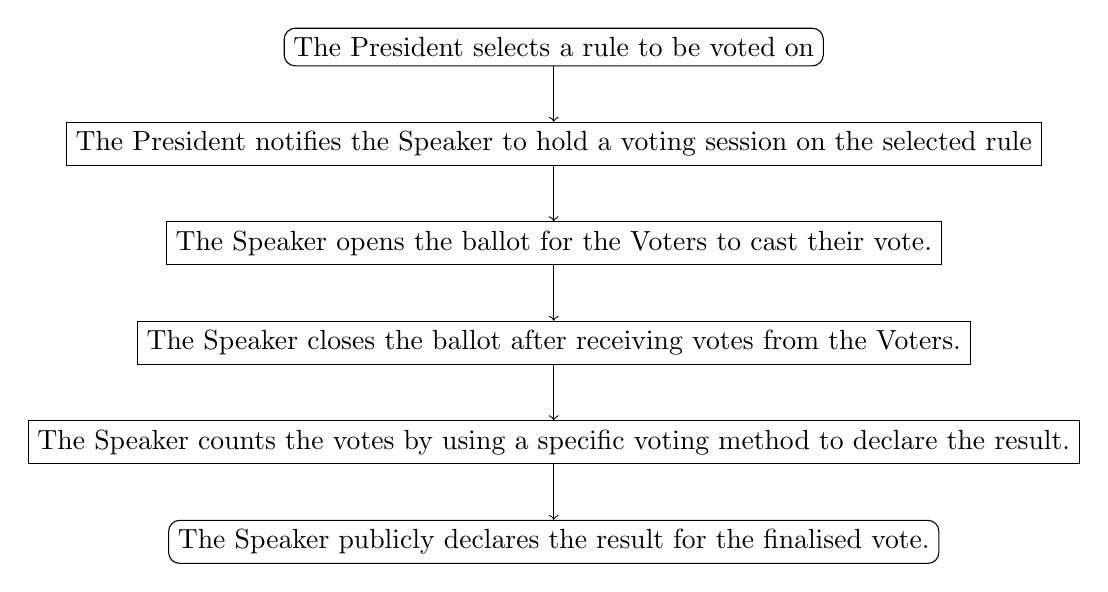
\begin{tikzpicture}[node distance=20pt]
\centering
\node[draw, rounded corners] (start)  {The President selects a rule to be voted on};
\node[draw, below=of start] (step 1)  {The President notifies the Speaker to hold a voting session on the selected rule};
\node[draw, below=of step 1] (step 2)  {The Speaker opens the ballot for the Voters to cast their vote.};
\node[draw, below=of step 2] (step 3)  {The Speaker closes the ballot after receiving votes from the Voters.};
\node[draw, below=of step 3] (step 4)  {The Speaker counts the votes by using a specific voting method to declare the result.};
\node[draw, below=of step 4, rounded corners] (end)   {The Speaker publicly declares the result for the finalised vote.};
 \draw[->] (start)  -- (step 1);
 \draw[->] (step 1) -- (step 2);
 \draw[->] (step 2) -- (step 3);
 \draw[->] (step 3) -- (step 4);
 \draw[->] (step 4) -- (end);
\end{tikzpicture}
\caption{Voting Protocol for Rules}
\label{fig:RONRVotingProtocol}
\end{center}
\end{figure}

For elections of roles, the sequence of actions of the voting protocol is mostly similar to the above explanation in principle, except for some parameters, such as the motion of the vote which is the role itself (President, or Speaker, or Judge), the facilitator of the election/vote event which depends on what role is being held for election (refer to Chapter 5 IIGO for more details on change of roles and power transfer), and the applicable voting method function to call for election that will produce the result, which is different from the voting method used for rules. Refer to Section~\ref{sec:VotingMethods} for more details on voting methods to be used for elections of roles.

At the start of the game, it is assumed that all 6 islands have the power to vote at any necessary voting scenario, and no diplomatic sanction is in place for any island. However, in the further turns of the game, some island(s) could lose their right to vote and/or not permitted to participate in a voting event due to the diplomatic sanction(s) in place. Refer to Chapter 5 IIGO for details on diplomatic sanction. In this case, the Speaker will open the ballots to the eligible islands only , i.e. those who are permitted to vote at a certain state of the game.

% Implmentaion section deleted

    \chapter{Team 1 Agent Design}

\section{Core Idea}
Team 1 agent was designed around the idea that the agent wants the whole archipelago to survive. However, the agent does have different configurations to allow for some malicious behaviour in order to facilitate some interesting agent interactions.

\section{Emotional state}

The agent's behaviour is affected by what we have termed her \emph{emotional state}. This is governed by the agent's current resources in relation to the living cost.

\begin{table} [htb]
    \centering
    \begin{tabular}{|l|l|}
        \hline
        \textbf{Emotional State} & \textbf{Condition} \\
        \hline
        Happy & Default state \\
        \hline
        Anxious & Current resources under 5 times the living costs \\
        \hline
        Desperate & Agent in critical state \\
        \hline
    \end{tabular}
\end{table}


\section{Opinions on Islands}
As information and resource sharing between islands is possible, it is possible and desirable for the agent to form an opinion of other islands. This be used to gauge the accuracy of information from other islands as well as, potentially, deny resource sharing to islands deemed ``selfish''.

Initially, opinion on all islands is neutral. Over time, through IITO and IIGO, opinions on islands will change. This will affect behaviour in IITO, as well as IIGO voting. Note that positive values correspond to positive opinions while negative values correspond to negative opinions.

\section{IITO Gifts}
When team 1 agent receives a request for gifts, the agent will decide how much to offer depending on the agent's current emotional state and the opinion of that island.

\begin{table} [htb]
    \centering
    \begin{tabular}{|c|p{0.5\textwidth}|}
        \hline
        \textbf{Emotional State} & \textbf{How is IITO handled?} \\
        \hline
        Happy & Agent will give away resources that satisfies the requested amount. Up to a percent of available resources. \\
        \hline
        Anxious & Agent will give away a ratio of the requested amount and its current resources. \\
        \hline
        Desperate & Agent will refuse any gift requests that it receives. \\
        \hline
    \end{tabular}
\end{table}

During IITO, the agent's opinion of other islands is affected. For every gift received, the agent's opinion of the gift-giver increases. However, the agent's opinion of an island can decrease if that island promised a gift and did not fulfil it.

Moreover, if the agent's opinion of an island is very high, the agent can decide to give gifts disregarding the agent's own anxiety. On the other hand, if an opinion of an island is very low, the agent can decide to refuse to send a gift even though the agent is happy.

For increase survivability, team 1 agent will accept any gift offers that it receives.

\subsection{Future Work}
Team 1 agent currently has a very straightforward IITO strategy. Possible alteration to this strategy could include:
\begin{itemize}
    \item Being less susceptible to bribery. The agent should stop increasing the opinion of an island after receiving $X$ amount of continuous gifts.
    \item Stop handing out gifts to islands that are not in critical state.
    \item Being proactive in bribery. The agent will give non-requested gifts to the current president in hopes that this will reduce tax and increase resource allocation from the common pool.
\end{itemize}

\section{IIFO Disaster Prediction}
Disasters can happen deterministically or stochastically (see Chapter~\ref{sec: Disaster} for more information). For an agent, it is important to predict when a disaster occurs so that as much disaster damage is mitigated using the common pool.

When the game starts, the disaster prediction made by the agent is random. This prediction always has a confidence value of $0$. As more disasters occur, a history of disasters is built up. Using this history, the mean disaster position ($x$, $y$), magnitude and period is calculated. A confidence value is calculated along with the mean disaster metrics and shared along with the prediction.

% Add a footnote on website?  https://www.mathsisfun.com/data/confidence-interval.html
The confidence value is calculated by finding the ratio between margin of error and the mean value. The smaller the margin of error, the more confident the agent is in her prediction. Therefore, a difference between the mean value and the margin of error must also be calculated. The confidence interval equation is used to calculate the margin of error:

\begin{equation}
    \label{eq: Team1MarginOfError}
    \textsc{Error} = Z \dfrac{s}{\sqrt{n}}
\end{equation}

where $s$, $n$ and $Z$ are the standard deviation, size of array and confidence interval respectively.

Using the difference between the mean value ($\bar{x}$) and the margin of error and taking the ratio of this result over the mean will provide the agent with the confidence value.
\begin{equation}
    \textsc{Confidence Value} = \frac{\bar{x} - \textsc{Error}}{\bar{x}}
\end{equation}.

The agent maintains a \textbf{trust score} for every island \emph{including itself}. This is based on the accuracy of islands' prediction of time left to the disaster.

Sharing and obtaining other disaster information to and from other islands respectively can increase the survivability of the archipelago. As more disaster predictions are shared, a network of trust between team 1 agent and other islands is built.

\subsection{Future Work}
While team 1 agent has a satisfactory disaster prediction algorithm, it does not make use of this prediction or predictions from other islands in any meaningful way. This is primarily due to disaster prediction being one of the last features to be implemented and not enough time being available to complete it.

Nevertheless, here are some possible uses for the disaster prediction system.

\begin{itemize}
  \item \textbf{Tax policy} --- As president, the agent could choose to increase or decrease taxation depending on (predicted) time left to disaster.
  \item \textbf{Voting} --- A trustworthy island could make for a better president, speaker or judge, as they would be able to act according to imminent disasters.
  \item \textbf{Common pool contribution} --- Based on predicted disaster location the agent may increase or decrease her common pool contribution. If a disaster is expected to affect the agent significantly then she could choose to mitigate resource loss by contributing a large amount to the common pool, as the alternative would be losing more resources.
\end{itemize}

Finally, prediction accuracy could be improved by using the prediction of the most trustworthy island, whether that is the agent herself or not, or averaging the predictions of the most trustworthy islands.

\section{IIGO: President}

Following the agent's core idea, as the president, the agent will try to enlarge the common pool as well as redistribute wealth among the islands, in an attempt to ensure the survival of as many islands as possible. This is achieved through an aggressive, tiered tax policy as well as denying common pool allocation requests to the wealthier islands.

This policy had to be verified as it could be vulnerable to ``free-rider'' islands, who could avoid paying tax and still reap the benefits of disaster protection from a large common pool and ``bailout'' allocations when they are low on resources.

As a test of this, a simulation was set up with a variable number of lawful and free-rider islands in order to measure the stability of this policy.

Three tax evading islands (half of the islands) was found to be the limit at which this policy would lead to collapse of the IIGO and the common pool. This was deemed an acceptable limit as at least half of the other agent teams would obey tax policy, at least most of the time or with a small amount of evasion. The resource graphs for the cases of two and three tax evading islands can be seen in \autoref{fig:team1:two_invaders} and \autoref{fig:team1:three_invaders}.

\begin{figure}[H]
\centering
\includegraphics[width=0.9\textwidth]{09_team1_agentdesign/images/two_invaders}
\caption{Resource graph. Islands 5 and 6 are evading tax.}
\label{fig:team1:two_invaders}
\end{figure}

\begin{figure}[H]
\centering
\includegraphics[width=0.9\textwidth]{09_team1_agentdesign/images/three_invaders}
\caption{Resource graph. Islands 4 to 6 are evading tax.}
\label{fig:team1:three_invaders}
\end{figure}

Note here that collapse of IIGO (as in \autoref{fig:team1:three_invaders}, with three tax evaders) does not automatically imply collapse of the archipelago; the islands appeared to survive (and, in fact, thrive) even after the collapse of IIGO.\@ It was taken as an assumption that this was only due to the uniformity of strategies, and in the ``real'' simulation, with heterogeneous agents, collapse of IIGO would lead to collapse of the archipelago.



\section{Foraging}
Multiple foraging strategies were developed, initially by intuition and later by attempting to address the shortcomings of previous attempts. They were developed in order and aptly named:
\begin{itemize}
    \item Return on Investment (ROI)
    \item Regression
    \item Flip Forage
\end{itemize}


\subsection{Return on Investment (ROI) Foraging}%
\label{sec:forage-roi}

This first algorithm is based on repeating successful foraging behaviours in the past, whether those be by the agent herself or another agent.

For the first few turns (the exact amount is configurable) the agent will forage randomly.

The agent maintains a history of foraging decisions and outcomes, including those received from IIFO.\@ When it comes time to forage, this history is sorted by ROI, i.e.\ the ratio of profit to contribution. Decisions that resulted in a loss, had profit smaller than the living cost, or had a larger contribution than a (configurable) percentage of available resources, are filtered out.

\subsection{Regression Foraging}%
\label{sec:forage-regression}

This strategy tries to predict the ideal foraging decision, even if that exact decision was not made in the past. This is done using regression, which is used to find the decision with the highest expected reward.

The \emph{regression} strategy forages randomly in the initial turns and history is kept as in \nameref{sec:forage-roi}. To make a foraging decision, the history is split by foraged resource (fish or deer), and quadratic regression is performed on contribution versus reward for both resources. From this, a quadratic equation is formed. If the quadratic equation found is negative then the optimal contribution can be found by differentiation. If it is positive then a (large) value is chosen as contribution, as a higher contribution should simply lead to a higher reward.

\subsection{Flip Foraging}

This strategy chooses the least foraged resource from the last turn, according to IIFO-reported data. Contributed amount is proportional to the chosen resource's total ROI from last turn. This choice was made under the assumption that ROI is an indicator of the resource's ``condition''. If a resource only gives moderate rewards (proportionally to input) it means that it is probably over-used currently and as such agents should allow it to recover, by scaling down their foraging attempts or by switching foraging types.

\subsection{Comparison}

To compare the three strategies, simulations were run with six agents, two using \emph{ROI foraging}, two using \emph{regression foraging}, and two using \emph{flip foraging}. IIGO and IITO were also disabled in order to isolate the efficacy of foraging methods from other parts of the game. The simulation was run five times and the results averaged over the 5 games as well as the two agents following the same strategy.

\begin{figure}[H] 
\centering
\includegraphics[width=0.6\textwidth]{09_team1_agentdesign/images/mean_survival_turns}
\caption{Mean survival turns for different strategies.}
\label{fig:team1:mean_survival}
\end{figure} 

\begin{figure}[H] 
\centering
\includegraphics[width=0.6\textwidth]{09_team1_agentdesign/images/total_efficiency}
\caption{Average foraging efficiency}
\label{fig:team1:average_efficiency}
\end{figure} 

It is clear from \autoref{fig:team1:mean_survival} that the \emph{flip} foraging strategy dominates the other two in terms of overall effectiveness. However, it is interesting to note that, according to \autoref{fig:team1:average_efficiency}, the \emph{ROI} foraging method is almost as efficient as \emph{flip}, which raises the question of what causes the difference in their success. This difference could be attributed to one core issue with the \emph{ROI strategy}: ignoring the absolute value of rewards. The agent will happily settle for a profit of $11$ resources, if that was obtained with a contribution of $0.1$ resources (a profit of $110000\%$) over a profit $50$ resources for a contribution of $25$ (a measly $100\%$). This means that in the long run living costs overwhelm the \emph{ROI} agent. The \emph{flip} agent does not take expected profit into account and as such is unaffected by this.

\emph{Regression} appears to occupy a medium between \emph{flip} and \emph{ROI}, however it is much less consistent, as evidenced by the error bars in \autoref{fig:team1:mean_survival}, with \emph{regression} surviving for under 10 turns in some runs.

%%% Local Variables:
%%% mode: latex
%%% TeX-master: "../main"
%%% End:

    \chapter{Inter-Island Governmental Organisation (IIGO)}


The role of IIGO is to maintain, update, and revise the rules concerning provision to managing the long-term collective risk dilemma (ltCRD). 

\begin{itemize}
    \item There will be 3 distinct branches in the IIGO: the \textbf{legislative branch}, \textbf{executive branch} and \textbf{judicial branch}\footnote{This is, as no surprise, inspired by the separation of powers in Western democracies.}.
    \item Each role is put in power according to the  transfer-of-power rules (see Section~\ref{subsec:transfer-of-power} for more detail).
    \item The head of the legislative branch is the Speaker, the head of the executive branch is the President, and the head of judicial branch is the Judge.
    \begin{itemize}
        \item  The Speaker, President and Judge are selected, through a democratic election, from the islands in the archipelago\footnote{This naming is inspired by the roles in the US Government.}.
        \item The resources gathered by the archipelago are endogenous, hence acting on the institutional powers granted to the Speaker, President or Judge costs resources. 
        \item For their duty, the President, the Speaker and the Judge receive a salary for each of their turns in office (see Section~\ref{subsec:salary} for more detail).
        \item The limit of the powers of the President, Speaker and Judge are defined in this chapter (e.g. the Speaker can only call one vote per turn).
 
    \end{itemize}
\end{itemize}

\subsection{IIGO Specific Definitions}
\begin{definition} \label{def:ballot}
    A \textbf{ballot} is related to each island's \textbf{power} to support or disagree with the rule specified in the vote called by the President and to vote in favour or against an island for a specific role (i.e. the President, Speaker, Judge) at each round of the game.
\end{definition}


%\begin{definition} \label{def:vote}
    %A \textbf{vote} is related to a role's (i.e. the President, Speaker, Judge) \textbf{power} to call a vote for a specific rule or an election.
%\end{definition}


\begin{definition} \label{def:tax}
    The \textbf{taxation} is related to the President's \textbf{power} to request a specific \underline{\textbf{minimum}} amount of contribution from each island to the common pool at each round of the game. 
\end{definition}

\begin{definition} \label{def:alloc_req}
    An \textbf{allocation request} is related to each island's \textbf{power} to request a specific amount of resource allocation from the President at each round of the game.
\end{definition}


\begin{definition} \label{def:rule_prop_list}
A \textbf{rule proposal list} is related to each island's \textbf{power} to propose a specific rule to be passed to the President at each round of the game.
\end{definition}

\begin{definition} \label{def:invst}
    An \textbf{investigation} is related to the Judge's \textbf{power} to acquire information to make a decision, followed by a calculation of the expected results and checking whether some specific rules have been obeyed, exclusively for the actions carried out by the \textbf{islands}. 
\end{definition}


An example of an \emph{investigation}: The President has permitted the island $X$ to take the amount of $Y$ resources from the common pool. Upon \emph{investigation} carried out by the Judge, it is revealed that the amount of resources taken out from the common pool by the island $X$ is, in fact, $Y'$ such that $Y' \neq Y$.


\begin{definition}
\textbf{Monitoring} is a government official's \textbf{power} to perform event recognition and to check whether some specific rules have been obeyed.
\end{definition}

An example of \emph{monitoring}: The Speaker has performed only the following action: \emph{counted the votes and calculated the result} for a rule. Upon \emph{monitoring} carried out by the President, it is noticed that the Speaker has not made any \emph{announcement}. Hence, the Speaker has not followed their obligation to \emph{announce} the result of any vote held.

See Section~\ref{sec:accountability} for more information about which roles can monitor which ones.


\begin{definition}
\textbf{Investigative-monitoring} is a government official's \textbf{power} to acquire the information used in acting on a governmental power followed by calculation of the expected results and checking whether some specific rules have been obeyed, exclusively for the actions carried out by a government official they are responsible for.
\end{definition}

An example of \emph{investigative-monitoring}: The Speaker has performed the following actions: \emph{counted the votes and calculated the result $R$} for a vote $V$ and \emph{announced} the result $R'$ for the vote $V$. Upon \emph{investigative-monitoring} carried out by the President, it is noticed that $R' \neq R$. Hence, the Speaker has modified the announced result.


\begin{definition}
The \textbf{sanction} is related to the Judge's \emph{power} to punish non-compliant islands when their disobedience is confirmed through investigations at a specific turn.
\end{definition}


\begin{definition}
The (judicial) \textbf{pardon} is related to the Judge's \emph{power} to forgive a non-compliant island at a specific turn.
\end{definition}

\begin{definition}
The \textbf{budget} is the maximum amount of resources a role is permitted to spend from the common pool as it performs its own institutional-power-enabled actions at a specific turn.
\end{definition}


\begin{definition}
The \textbf{salary} is the amount of resources a role is to be given from the common pool as a reward for performing its institutional-power-enabled actions at a specific turn.
\end{definition}

\begin{definition} \label{def:term}
A \textbf{term} is the number of turns an island is \emph{permitted} to hold a role, and after which the responsible role (indicated in the transfer-of-power cycle in Figure~\ref{fig:cycles_in_IIGO}) is \emph{obliged} to initiate transfer-of-power.
\end{definition}

\subsection{\emph{Power}, \emph{Permission} and \emph{Obligation} Distinction}
In the rest of the specifications, we will be specifically using the following three terms to define the actions and responsibilities carried out by the Speaker, President, Judge (see Figure~ \ref{fig:per_obl_sets}):
\begin{itemize}
    \item Power
    \item Permission
    \item Obligation
\end{itemize}



\begin{figure}[H] 
\centering
\includegraphics[width=0.6\textwidth]{05_iigo/images/SOMAS_per_obl.pdf}
\caption{Relationship between \emph{power}, \emph{permission} and \emph{obligation}.}
\label{fig:per_obl_sets}
\end{figure} 


For example, the Judge has the \emph{power} to carry out investigations at an IIGO session. There are no rules specifying which specific islands the Judge should investigate. Therefore, the Judge has the \emph{permission} to investigate any `alive' islands during a session. However, the Judge is \emph{obliged} to make at least some number of investigations each turn.



\section{Executive Branch}
\label{sec:executive}
The executive branch is responsible for \textbf{carrying out the law}.
\begin{itemize}
       
    \item The President has the \emph{power} to: 
    \begin{itemize}
        
        \item Select a rule for voting $R^{*}$ to be passed to the Speaker.
        \begin{rule_IIGO}
            The President has the \emph{obligation} to \emph{select} a rule $R^{*}$ if the \emph{rule proposal list} has at least one proposed rule in it.
        \end{rule_IIGO}
        \begin{rule_IIGO}
            The President has the \emph{permission} to \emph{select} a rule $R^{*}$ if and only if $R^{*} \in S$, where $S$ is the \emph{rule proposal list}.
        \end{rule_IIGO}
        
        \item Decide the amount of individual \emph{taxation} (i.e. a specific \emph{minimum} amount of contribution to the common pool for each island) for the current turn.
        
        \begin{itemize}
            \item The President is given the self-reported resource amounts held by each island to assist in this decision.
            %\item Suggested Rule: For any island that has chosen to not report it's resources, the President has the \emph{obligation} to set them an individual tax amount T.
        \end{itemize}
        
        \item Decide the allocation of resources distributed from the common pool to the islands (i.e. a specific \emph{maximum} amount an island is permitted to take from the common pool).
        
        \begin{itemize}
            \item The President is given the \emph{allocation requests} made by each island.
            %\item \emph{}{Suggested Rule:} The President has an obligation to prioritise islands in critical condition.
        \end{itemize}
    \end{itemize}
\end{itemize}



\section{Legislative Branch}
\label{sec:legislative}
The legislative branch is responsible for \textbf{making the law}.
\begin{itemize}

    \item The Speaker has the \emph{power} to:
    \begin{itemize}
        
        \item Call a vote $V$ for a rule $R$.
        \begin{rule_IIGO}
            The Speaker has the \emph{obligation} to \emph{call} a vote $V$ if and only if the President has \emph{selected} a rule $R$ to be voted on.
        \end {rule_IIGO}
        \begin{rule_IIGO}
            The Speaker has the \emph{permission} to \emph{call} a vote $V$ for a rule $R$ if and only if the rule $R = R^{*}$, where $R^{*}$ is the rule \emph{selected} by the President.
        \end {rule_IIGO}
            
        \item Choose which islands are participating in the vote $V$.
       % \footnote{This is our sequential implementation alternative for the power to close the ballot box.}.
        \begin{rule_IIGO}
            The Speaker has the \emph{obligation} to ask for a vote from all alive islands.
        \end {rule_IIGO}
            
        \item Declare the result $C$ of a vote $V$. 
        \begin{rule_IIGO}
            The Speaker has the \emph{obligation} to \emph{declare the result} $C$ for a vote $V$ if and only if the vote V has been \emph{called}.
        \end {rule_IIGO}
        \begin{rule_IIGO}
            The Speaker has the \emph{permission} to \emph{declare the result} $C$ for a vote $V$ if $C = C^{*}$, where $C^{*}$ is the result produced by \emph{calling} the vote $V$.
        \end {rule_IIGO}
        \begin{itemize}
            \item This step is what enables a rule to be \emph{active}.
        \end{itemize}
    \end{itemize}
\end{itemize}




\section{Judicial Branch}
\label{sec:judicial}

The judicial branch is responsible for \textbf{evaluating the law}.
\begin{itemize}
    \item The Judge has the \emph{power} to:
    \begin{itemize}
        \item Perform a number of \emph{inspections}\footnote{An \emph{inspection} \textbf{costs} an expense of resources (See Definition~\ref{def:invst} for more detail).} $I$ and produce a compliance outcome $\mathbb{O}^{*}$\footnote{Note that the compliance outcome $\mathbb{O}^{*}$ considered is a boolean.}.
        %(true: the island has been compliant with the rules in play, false: the island has not been compliant with the rules in play)
        %\begin{itemize}
           % \item For example, to check if the event outcome is \emph{concurrent}\footnote{Again, what is defined as "concurrent"? A clear definition is needed.} with the rules.
        %\end{itemize}
        \begin{rule_IIGO}
            The Judge has the \emph{obligation} to make at least $N$ investigations at each turn.
        \end{rule_IIGO}
        \item Declare the outcome $\mathbb{O}$ of an inspection $I$ to all islands\footnote{This act of broadcasting is especially important for islands to form an opinion about the sanctioned islands accordingly.}.
        \begin{rule_IIGO}
            The Judge has the \emph{obligation} to declare the outcome $\mathbb{O}$ of an inspection $I$ if and only if the inspection $I$ has been performed.
        \end{rule_IIGO}
        \begin{rule_IIGO}
            The Judge has the \emph{permission} to declare the outcome $\mathbb{O}$ of an inspection $I$ if $\mathbb{O} = \mathbb{O}^{*}$, where $\mathbb{O}^{*}$ is the outcome of the inspection $I$.
        \end{rule_IIGO}
        %\item Initiate the removal of the \texttt{President}.
        %\begin{itemize}
            %\item A good Judge would be especially vigilant during \emph{power transfer} regarding the \emph{President} position (see Section~\ref{leg_const} for more detail).
        %\end{itemize}
        \item Invoke economic \textbf{sanctions} (see Section~\ref{sec:sanctions} for more detail).
        \begin{rule_IIGO}
            The Judge has the \emph{obligation} to invoke a sanction $S$ for an island $X$ if and only if an investigation $I$ has an outcome $\mathbb{O}^{*}$ indicating non-compliance, and $I$ is an investigation of an action taken by island $X$.
        \end{rule_IIGO}
        \item Invoke even more severe sanctions in the case of further disobedience to previous sanction(s).
        \begin{rule_IIGO}
            The Judge has the \emph{permission} to invoke a severer sanction $S'$ for an island $X$ if the island $X$ has not fulfilled the requirements of the previous sanction $S$.
        \end{rule_IIGO}
        \item Pardon the islands which are currently sanctioned.
        \begin{rule_IIGO}
            The Judge has the \emph{permission} to revoke any sanction $S$ of an island $X$ at a specific turn.
        \end{rule_IIGO}
    \end{itemize}
\end{itemize}
%(e.g. a new rule that falls under a "sanction" category \hl{[I'm not sure about this being a `new rule` [Ezgi]]}

\subsection{Sanctions}
\label{sec:sanctions}
All sanctions are of economic nature which include:
        \begin{itemize}
            %\item Revoking an island's access to the common pool.
            \item Enforcing an island to contribute a specific amount of resources to the common pool.
            \begin{itemize}
                \item This does not mean that the Judge has the \emph{power} to take resources from an island in order to put them to the common pool -- the island itself is expected to carry out this implication imposed by the sanction itself, otherwise further punishment can be induced by the Judge.
                \item Similarly, \emph{opinion formulation} will follow accordingly whether the island(s) is/are following the implications imposed by the sanction(s).
            \end{itemize}
        
    \end{itemize}
    Sanctions are the associated penalty that comes with an island breaking a specific rule. The Judge is in full control of the penalties associated with breaking any rules. Once the Judge has specified the score of the penalty associated with each time an island breaks a rule, the cumulative penalties accumulated by the island are then used to determine which \textbf{sanction tier} that each island falls into. The score threshold to determine the boundaries of the sanction tiers are set by the Judge. At each turn of the game, each island is told whether they are being sanctioned, and if so, which \textbf{sanction tier} that they are currently in. The \textbf{sanction tiers} of the non-compliant islands are also broadcasted to the other islands in the archipelago. To summarise, the sanctioning process follows these steps:
    
    
    
    %Sanctions are based on an island breaking a rule. Each rule must therefore have an associated penalty. By default, we set these penalties such that they add $1$ to the total sanction score for each island. However, we allow the judge to override this scoring, the judge is able to set their own scores for any particular rule as they desire. This custom scoring is then used when an island breaks a particular rule. By looking at events that occurred in the last turn, and using the customised scoring we provide the holder of the judge role with full control of the penalties for breaking any rules.
    
    





%we then use the cumulative penalties accumulated by each island to determine which Sanction Tier they fall into. The score threshold's required to fall into these sanction tiers is set by the judge and is checked for monotonicity. Each island is told whether they are being sanctioned, and is so what tier they are in. We also tell other islands about which sanction tiers other islands have fallen into. 

    \begin{enumerate}
        \item The Judge has the \emph{power} to set custom penalties associated with breaking any rules.
        \item The Judge is given a list of all events that occurred in the previous turn.
        \item The Judge has the \emph{power} to check whether any, or all of these previous events, involve the islands in the archipelago breaking any rules.
        \item Each of the transgressions is scored using the Judge's custom penalties if the Judge has set them. Otherwise, a score of $1$ is given each time a rule is broken.
        \item The Judge has the \emph{power} to revise the sanction thresholds.
        \item Using the latest sanction thresholds available, each island is assigned to a sanction tier based on the sanction score that it has received.
        \item These sanction tiers are broadcasted to all of the islands in the archipelago.
        \item The Judge then uses sanctions rules in place to calculate the specific amount of resources that each non-compliant island has in order to determine how much it should contribute to the common pool, based on the sanction tier that it is in.
    \end{enumerate}



\section{Constitutional Rights and Obligations in the Archipelago}
\label{sec:const_rights_obl_archi}
Each island has the \emph{power} to:
\begin{itemize}
\item make an \emph{allocation request} (see Definition~\ref{def:alloc_req}) to the President for a specific amount to be allocated to them.
\item report the number of resources it is in possession of to the President.
\begin{rule_IIGO}
    Each island has the \emph{obligation} to report the number of resources it is in possession of to the President.
\end{rule_IIGO}
\begin{rule_IIGO}
    Each island has the \emph{permission} to report the number of resources $R'$ if and only if $R' = R$, where R is the number of resources the island is in possession of.
\end{rule_IIGO}
\item take resources from the common pool.


\begin{rule_IIGO}
    Each island has the \emph{permission} to take at maximum $N$ resources, where $N$ is the specific allocation made by the President to that island\footnote{If no such allocation is made, the island is \emph{permitted} to take any amount of resources.}.
\end{rule_IIGO}
\item contribute resources to the common pool.
\begin{rule_IIGO}
    Each island has the \emph{obligation} to contribute to the common pool an amount greater or equal to that of the individual tax set by the President.
\end{rule_IIGO}
                %The President is in
                %(unless there is a rule in place that dictates how Speaker is to allocate resources).
\item add a rule to the \emph{rule proposal list} (see Definition~\ref{def:rule_prop_list}) at the start of each turn.
        %\begin{itemize}
            %\item The game specification includes how many rules an island can propose each turn.
        %\end{itemize}
        %\item vote  for rules in the Legislative Branch and vote for their favourite islands in elections
\item participate in the legislative branch of the government by casting ballots in votes called by the Speaker
\item vote for an island to be elected for a specific role (e.g. the President, Judge, Speaker) during the elections\footnote{This will be assumed to be true \underline{unless stated otherwise}. %Note that \textbf{diplomatic sanctions} can disable this power of a specific island (see Section~\ref{jud_const}).}.
        }.
\end{itemize}
\section{Accountability Cycle}
\label{sec:accountability}


To ensure that the government avoids corruption and abuse of power, each branch is accountable to another. The President is accountable to the Speaker, the Speaker is accountable to the Judge, and the Judge is accountable to the President (see Figure~ \ref{fig:cycles_in_IIGO}). This accountability cycle is enacted through \emph{monitoring} actions\footnote{Note that the terms \textbf{monitoring} and \textbf{investigation} have similar but quite different meanings in the IIGO context.}. 

The powers related to the accountability cycle and transfer-of-power for each role can be summarized as the following: 
\begin{itemize}
    \item The Speaker has the \emph{power} to: 
    \begin{itemize}
        \item monitor the President.
        \item announce the result of this monitoring.
        \item initiate the transfer-of-power for the Judge.
    \end{itemize}
    \item The President has the \emph{power} to: 
    \begin{itemize}
        \item monitor the Judge.
        \item announce the result of this monitoring.
        \item initiate the transfer-of-power for the Speaker.
    \end{itemize}
    \item The Judge has the \emph{power} to: 
    \begin{itemize}
        \item  monitor the Speaker.
        \item announce the result of this monitoring.
        \item initiate the transfer-of-power for the President.
    \end{itemize}
\end{itemize}

%Unlike investigations performed by the Judge, who performs investigations on island actions in the following turn, each role is given the opportunity to check up on the actions of the role it is responsible for immediately after they have been performed. In this sense, the President can monitor (includes investigative-monitoring) the powers (calling a vote and announcing the result) acted on by the Speaker immediately after the Speaker's announcement (or lack there of). The government officials hold a lot of power so this is to ensure that any wrong-doing is determined as quickly as possible. For this project we are only pursuing one degree of monitoring, that is, the powers relating to the accountability cycle will not be monitored themselves. We assume that agents will act in the interest of themselves and keeping all the islands alive is beneficial to everyone. Hence, while the agents might be inclined to break rules in order to benefit themselves, anyone else breaking the rules is seen as undesirable under the assumption that the system in place is there to benefit all. 


Through the proposed accountability cycle, each role is given the opportunity to check up on the actions of the role it is accountable for immediately after they have been performed. It is clear that the IIGO roles (i.e. the President, Speaker and Judge) hold a considerable amount of \emph{power} in their hands. The accountability cycle is designed to address the possible abuses of this power. With monitoring, any wrong-doing in the IGO is determined as quickly as possible and the role in question can be replaced. 

Within the scope of the coursework, we decided to pursue only \emph{one degree of monitoring}, meaning that the powers relating to the accountability cycle will not be monitored themselves. We assume that agents will act in the interest of all the islands in the archipelago. Hence, while the agents might be inclined to break the rules to benefit in some form, it is assumed that the others will negatively see any non-compliant islands based on the assumption that the proposed IIGO system is in place to maintain the welfare of all the islands.

Let role $X$ be accountable to the role $Y$, which is accountable to the role $Z$. Then:
\begin{rule_IIGO}
$Y$ has the \emph{obligation} to declare the outcome of the monitoring result $M$ associated with the action $A$ undertaken by $X$ if and only if $Y$ has monitored the action $A$ performed by $X$. 
\end{rule_IIGO}
\begin{rule_IIGO}
$Y$ has the \emph{permission} to declare the monitoring result $M$ associated with the action $A$ undertaken by $X$ if and only if $M = M^{*}$, where $M^{*}$ is the outcome of \emph{monitoring} action $A$ performed by $X$\footnote{These constitutional rules should be available to the agents to check their decision against. However, due to having only one degree of accountability cycle in place, these rules are not enforced through any sanctions (i.e. breaking these rules has no consequences as they only deem to be an \emph{agreement} among the roles).}.
\end{rule_IIGO}


\begin{figure}[!htb]
\centering
\includegraphics[scale=0.33]{05_iigo/images/role cycles.png}
\caption{Accountability cycle (left), the transfer-of-power cycle (middle) and salary cycle (right).}
\label{fig:cycles_in_IIGO}
\end{figure}


\subsection{Transfer-of-power}
\label{subsec:transfer-of-power}
\begin{enumerate}
    \item The Speaker conducts a vote for the election of the new Judge.
    \item The Judge conducts a vote for the election of the new President.
    \item The President conducts a vote for the election of the new Speaker.
\end{enumerate}
Refer to the Figure~ \ref{fig:cycles_in_IIGO} for further clarification about the transfer-of-power cycle.

\begin{rule_IIGO}
   The role $X$ has the \emph{obligation} to conduct a vote for the election of $Y$ at the end of the term (see Definition~\ref{def:term}) if and only if the role $X$ is accountable to the role $Y$. 
\end{rule_IIGO}.

\section{Budget and Salary}
\subsection{Budget}
%Actions associated with the IIGO have an associated cost that is defined as a configuration parameter. The institutional-power-enabled actions of  identified to require a "computational" component are:

Institutional-enabled-power actions in the IIGO have an associated cost with them. Some examples for such actions include:


%that is defined as a configuration parameter. The institutional-power-enabled actions of  identified to require a "computational" component are:


%We have defined the resource to be an endogenous one, hence any computation surrounding the distribution of the resource must use up some of that resource. 
\begin{itemize}
\item Calling any vote and computing the winner.
\item Declaring (e.g. \textit{announcing} the result of a vote).
\item Setting the amount of \emph{taxation} for each island.
\item Deciding the allocation distribution for each island.
\item Inspecting an island's action history.
\item Monitoring a role.
\end{itemize}

Since IIGO has been designed to act in the common good, IIGO-related costs will be directly withdrawn from the common pool. Since the common pool is considered a communal property of the archipelago, there are rules in place to limit how much each role is allowed to spend in order to perform its own institutional-power-enabled actions. This is the reason why defining the \emph{budget} and keeping it separate for each of the three IIGO roles.


As a role performs institutional-enabled-power actions, the corresponding cost associated with this action is subtracted from the role's budget. A budget of zero means that the role does not have the \emph{power} to perform any of its institutional-power-enabled actions. The removal of the budget rule from the rules in play means the role is allowed to perform as many such actions as it prefers to (as long as those actions are not governed by other rules). 



%As a role performs an endogenous-cost action, the corresponding cost associated with this action is subtracted from the role's budget. Thus, if as a result of an endogenous-cost action a role will be left with negative budget, it will have gone over the budget limit and will have broken the budget rule. A budget of zero means that the role is not allowed to perform any of its institutional-power-enabled actions associated an endogenous-cost. The removal of the budget rule from the rules in play means the role is allowed to perform as many such actions as it pleases (as long as those actions are not governed by other rules). 

The budget rule is also persistent across turns. This means that, assuming nothing else affects the budget, if a role has $100$ resources in its budget at each turn and spends only $10$ resources, this means that this very same role has $90$ resources in its budget at the next turn. On the other hand, islands can choose to increase the budget periodically every turn. This is governed by another budget extension rule.




%one turn and it spends 10, it has 90 resources in it's budget the next turn. 

Finally, it must be noted that the budget is inherently linked with the fact that whether obligations of a specific role can be undergone.
For example, during \emph{monitoring}, it should not be seen as a rule violation if a role has not acted on an obligation if it would go over the budget as a result. 

%This can also be seen as an added clause "... and the action is only permitted if they have the budget" to most rules which govern actions with an endogenous-cost.
%\begin{rule_IIGO}
    %The budget is increased by an amount $N$ every turn.
%\end{rule_IIGO}

%This rule means that, assuming nothing else affects the budget, if a budget is set to increase by 10 resources every turn and the budget is a 100 resources in turn one, the budget is 110 resources in turn 2. Setting this rule to 0 is equal to removing this rule and it means that the budget is never increased. 


\subsection{Salary}
\label{subsec:salary}
A salary is paid to each role in power as an incentive to act in a publicly approved way. %Hence, each role has the \emph{power} to pay a salary to another role following the salary cycle in Figure~\ref{fig:cycles_in_IIGO}.
\begin{rule_IIGO} \label{rule:salary}
   %Each role has the \emph{obligation} to pay the salary of amount $S$ to another if and only if the amount paid $S'$ is equal to $S$.
   Each role has the \emph{obligation} to pay the salary of amount $S$ to one another following the salary cycle in Figure~\ref{fig:cycles_in_IIGO}.
\end{rule_IIGO}

In Rule~\ref{rule:salary}, setting $S=0$ (through changing the active rules in place) means that roles do not have the permission to pay any salary. Removing the Rule~\ref{rule:salary} means that the roles may freely choose the amount $S$ for the salary payments.

\section{IIGO Session order}

\begin{enumerate}
    \item The Judge has the \emph{power} to check the history of actions to confirm whether the previously punished island(s) has/have obeyed the previous round's sanctions, meaning whether they contributed to the common pool accordingly in case of economic sanctions.
    %\begin{itemize}
      %  \item \emph{Suggested Rule:} In case of disobeying sanctions, the Judge is \emph{obliged} and \emph{permitted} to increase the severity of sanctions with respect to specific islands.
   % \end{itemize}
    \item The Judge has the \emph{power} to carry out \emph{inspections} on the history of actions of any island $X$ to check whether:
        \begin{enumerate}
        \item the reported resources of $X$ in the previous round match the real value of resources $X$ had in its private pool for the previous turn.
        \item the island $X$ has retrieved the right amount of the resources from the common pool, based on the \emph{allocation request} evaluated by the previous President.
            \begin{itemize}
            \item An example: In the previous round, the President has decided that the island $X$ can take $Y$ amount of resources from the common pool. If the Judge finds out that the island $X$ has taken an amount of $Y'$ such that $Y' > Y$, the Judge has the \emph{power} to invoke sanctions on the island $X$.
            
            %the Judge is \emph{obliged} and \emph{permitted} to sanction island $X$.
            \end{itemize}
        \end{enumerate}
    \item The Judge has the \emph{power} to invoke sanctions based on the outcome of the inspections.
    \item The President has the \emph{power} to decide to carry out a \emph{monitoring} on:
        \begin{enumerate}
        \item the sanctions imposed by the Judge.
        \end{enumerate}
    \item The islands may report the resources in their private pools to the President.
    \item The President has the \emph{power} to let each island know about the amount of \emph{taxation} they have to pay.
    \item The island has the \emph{power} to make an \emph{allocation request} to the President.
    \item The President has the \emph{power} decide on an allocation of resources and let each island know about the amount of resource allocation they are permitted to take from the common pool.
    \item The island has the \emph{power} to pick and to propose a rule to be voted on to the President.
    \item The President has the \emph{power} to choose a rule to be voted on from the received rule proposals.
    \item The Speaker has the \emph{power} to decide to carry out a \emph{monitoring} on: 
        \begin{enumerate}
        \item the resource allocation decided by the President.
        \item the rule proposed by the President.
        \end{enumerate}
    \item The Speaker has the \emph{power} to call a vote.
        \begin{enumerate}
        \item The islands vote in support of, or against, the rule (aye or nay) anonymously.
        \end{enumerate}
    \item The Speaker has the \emph{power} to announce a result of a vote to the islands and carries out the law change, if required (e.g. deleting/rejecting a rule if there is a majority nay vote).
    \item The Judge has the \emph{power} to decide to carry out \emph{monitoring} on:
        \begin{enumerate}
        \item the vote called by the Speaker.
        \item the Speaker announcing the result.
    \end{enumerate}
    \item The roles pay salary for one another following the accountability cycle in Figure~ \ref{fig:cycles_in_IIGO}.

\end{enumerate}



\section{Future Work}

\begin{itemize}
    \item \textbf{Diplomatic sanctions}: Although having the potential of being a good alternative for severer sanctions discussed in  Section~\ref{sec:sanctions}, diplomatic sanctions are \emph{not} implemented within the scope of the coursework. \\
    Suggested diplomatic sanctions include:
        \begin{itemize}
            \item Revoking an island's eligibility to vote and to be elected for a position.
            \item Revoking an island's eligibility to propose a rule/motion.
        \end{itemize}
    \item \textbf{Immutable rules}: Within the scope of the coursework, a subset of rules could have been categorised as immutable. This means that to change such immutable rules, the islands first need to vote to change their status to be \emph{mutable}, and consequently, hold another vote to change these mutable rules.
    %\item \textbf{Adding rules to the proposal list: } 
\end{itemize}

    \chapter{Inter-Island Governmental Organisation (IIGO)}


The role of IIGO is to maintain, update, and revise the rules concerning provision to managing the long-term collective risk dilemma (ltCRD). 

\begin{itemize}
    \item There will be 3 distinct branches in the IIGO: the \textbf{legislative branch}, \textbf{executive branch} and \textbf{judicial branch}\footnote{This is, as no surprise, inspired by the separation of powers in Western democracies.}.
    \item Each role is put in power according to the  transfer-of-power rules (see Section~\ref{subsec:transfer-of-power} for more detail).
    \item The head of the legislative branch is the Speaker, the head of the executive branch is the President, and the head of judicial branch is the Judge.
    \begin{itemize}
        \item  The Speaker, President and Judge are selected, through a democratic election, from the islands in the archipelago\footnote{This naming is inspired by the roles in the US Government.}.
        \item The resources gathered by the archipelago are endogenous, hence acting on the institutional powers granted to the Speaker, President or Judge costs resources. 
        \item For their duty, the President, the Speaker and the Judge receive a salary for each of their turns in office (see Section~\ref{subsec:salary} for more detail).
        \item The limit of the powers of the President, Speaker and Judge are defined in this chapter (e.g. the Speaker can only call one vote per turn).
 
    \end{itemize}
\end{itemize}

\subsection{IIGO Specific Definitions}
\begin{definition} \label{def:ballot}
    A \textbf{ballot} is related to each island's \textbf{power} to support or disagree with the rule specified in the vote called by the President and to vote in favour or against an island for a specific role (i.e. the President, Speaker, Judge) at each round of the game.
\end{definition}


%\begin{definition} \label{def:vote}
    %A \textbf{vote} is related to a role's (i.e. the President, Speaker, Judge) \textbf{power} to call a vote for a specific rule or an election.
%\end{definition}


\begin{definition} \label{def:tax}
    The \textbf{taxation} is related to the President's \textbf{power} to request a specific \underline{\textbf{minimum}} amount of contribution from each island to the common pool at each round of the game. 
\end{definition}

\begin{definition} \label{def:alloc_req}
    An \textbf{allocation request} is related to each island's \textbf{power} to request a specific amount of resource allocation from the President at each round of the game.
\end{definition}


\begin{definition} \label{def:rule_prop_list}
A \textbf{rule proposal list} is related to each island's \textbf{power} to propose a specific rule to be passed to the President at each round of the game.
\end{definition}

\begin{definition} \label{def:invst}
    An \textbf{investigation} is related to the Judge's \textbf{power} to acquire information to make a decision, followed by a calculation of the expected results and checking whether some specific rules have been obeyed, exclusively for the actions carried out by the \textbf{islands}. 
\end{definition}


An example of an \emph{investigation}: The President has permitted the island $X$ to take the amount of $Y$ resources from the common pool. Upon \emph{investigation} carried out by the Judge, it is revealed that the amount of resources taken out from the common pool by the island $X$ is, in fact, $Y'$ such that $Y' \neq Y$.


\begin{definition}
\textbf{Monitoring} is a government official's \textbf{power} to perform event recognition and to check whether some specific rules have been obeyed.
\end{definition}

An example of \emph{monitoring}: The Speaker has performed only the following action: \emph{counted the votes and calculated the result} for a rule. Upon \emph{monitoring} carried out by the President, it is noticed that the Speaker has not made any \emph{announcement}. Hence, the Speaker has not followed their obligation to \emph{announce} the result of any vote held.

See Section~\ref{sec:accountability} for more information about which roles can monitor which ones.


\begin{definition}
\textbf{Investigative-monitoring} is a government official's \textbf{power} to acquire the information used in acting on a governmental power followed by calculation of the expected results and checking whether some specific rules have been obeyed, exclusively for the actions carried out by a government official they are responsible for.
\end{definition}

An example of \emph{investigative-monitoring}: The Speaker has performed the following actions: \emph{counted the votes and calculated the result $R$} for a vote $V$ and \emph{announced} the result $R'$ for the vote $V$. Upon \emph{investigative-monitoring} carried out by the President, it is noticed that $R' \neq R$. Hence, the Speaker has modified the announced result.


\begin{definition}
The \textbf{sanction} is related to the Judge's \emph{power} to punish non-compliant islands when their disobedience is confirmed through investigations at a specific turn.
\end{definition}


\begin{definition}
The (judicial) \textbf{pardon} is related to the Judge's \emph{power} to forgive a non-compliant island at a specific turn.
\end{definition}

\begin{definition}
The \textbf{budget} is the maximum amount of resources a role is permitted to spend from the common pool as it performs its own institutional-power-enabled actions at a specific turn.
\end{definition}


\begin{definition}
The \textbf{salary} is the amount of resources a role is to be given from the common pool as a reward for performing its institutional-power-enabled actions at a specific turn.
\end{definition}

\begin{definition} \label{def:term}
A \textbf{term} is the number of turns an island is \emph{permitted} to hold a role, and after which the responsible role (indicated in the transfer-of-power cycle in Figure~\ref{fig:cycles_in_IIGO}) is \emph{obliged} to initiate transfer-of-power.
\end{definition}

\subsection{\emph{Power}, \emph{Permission} and \emph{Obligation} Distinction}
In the rest of the specifications, we will be specifically using the following three terms to define the actions and responsibilities carried out by the Speaker, President, Judge (see Figure~ \ref{fig:per_obl_sets}):
\begin{itemize}
    \item Power
    \item Permission
    \item Obligation
\end{itemize}



\begin{figure}[H] 
\centering
\includegraphics[width=0.6\textwidth]{05_iigo/images/SOMAS_per_obl.pdf}
\caption{Relationship between \emph{power}, \emph{permission} and \emph{obligation}.}
\label{fig:per_obl_sets}
\end{figure} 


For example, the Judge has the \emph{power} to carry out investigations at an IIGO session. There are no rules specifying which specific islands the Judge should investigate. Therefore, the Judge has the \emph{permission} to investigate any `alive' islands during a session. However, the Judge is \emph{obliged} to make at least some number of investigations each turn.



\section{Executive Branch}
\label{sec:executive}
The executive branch is responsible for \textbf{carrying out the law}.
\begin{itemize}
       
    \item The President has the \emph{power} to: 
    \begin{itemize}
        
        \item Select a rule for voting $R^{*}$ to be passed to the Speaker.
        \begin{rule_IIGO}
            The President has the \emph{obligation} to \emph{select} a rule $R^{*}$ if the \emph{rule proposal list} has at least one proposed rule in it.
        \end{rule_IIGO}
        \begin{rule_IIGO}
            The President has the \emph{permission} to \emph{select} a rule $R^{*}$ if and only if $R^{*} \in S$, where $S$ is the \emph{rule proposal list}.
        \end{rule_IIGO}
        
        \item Decide the amount of individual \emph{taxation} (i.e. a specific \emph{minimum} amount of contribution to the common pool for each island) for the current turn.
        
        \begin{itemize}
            \item The President is given the self-reported resource amounts held by each island to assist in this decision.
            %\item Suggested Rule: For any island that has chosen to not report it's resources, the President has the \emph{obligation} to set them an individual tax amount T.
        \end{itemize}
        
        \item Decide the allocation of resources distributed from the common pool to the islands (i.e. a specific \emph{maximum} amount an island is permitted to take from the common pool).
        
        \begin{itemize}
            \item The President is given the \emph{allocation requests} made by each island.
            %\item \emph{}{Suggested Rule:} The President has an obligation to prioritise islands in critical condition.
        \end{itemize}
    \end{itemize}
\end{itemize}



\section{Legislative Branch}
\label{sec:legislative}
The legislative branch is responsible for \textbf{making the law}.
\begin{itemize}

    \item The Speaker has the \emph{power} to:
    \begin{itemize}
        
        \item Call a vote $V$ for a rule $R$.
        \begin{rule_IIGO}
            The Speaker has the \emph{obligation} to \emph{call} a vote $V$ if and only if the President has \emph{selected} a rule $R$ to be voted on.
        \end {rule_IIGO}
        \begin{rule_IIGO}
            The Speaker has the \emph{permission} to \emph{call} a vote $V$ for a rule $R$ if and only if the rule $R = R^{*}$, where $R^{*}$ is the rule \emph{selected} by the President.
        \end {rule_IIGO}
            
        \item Choose which islands are participating in the vote $V$.
       % \footnote{This is our sequential implementation alternative for the power to close the ballot box.}.
        \begin{rule_IIGO}
            The Speaker has the \emph{obligation} to ask for a vote from all alive islands.
        \end {rule_IIGO}
            
        \item Declare the result $C$ of a vote $V$. 
        \begin{rule_IIGO}
            The Speaker has the \emph{obligation} to \emph{declare the result} $C$ for a vote $V$ if and only if the vote V has been \emph{called}.
        \end {rule_IIGO}
        \begin{rule_IIGO}
            The Speaker has the \emph{permission} to \emph{declare the result} $C$ for a vote $V$ if $C = C^{*}$, where $C^{*}$ is the result produced by \emph{calling} the vote $V$.
        \end {rule_IIGO}
        \begin{itemize}
            \item This step is what enables a rule to be \emph{active}.
        \end{itemize}
    \end{itemize}
\end{itemize}




\section{Judicial Branch}
\label{sec:judicial}

The judicial branch is responsible for \textbf{evaluating the law}.
\begin{itemize}
    \item The Judge has the \emph{power} to:
    \begin{itemize}
        \item Perform a number of \emph{inspections}\footnote{An \emph{inspection} \textbf{costs} an expense of resources (See Definition~\ref{def:invst} for more detail).} $I$ and produce a compliance outcome $\mathbb{O}^{*}$\footnote{Note that the compliance outcome $\mathbb{O}^{*}$ considered is a boolean.}.
        %(true: the island has been compliant with the rules in play, false: the island has not been compliant with the rules in play)
        %\begin{itemize}
           % \item For example, to check if the event outcome is \emph{concurrent}\footnote{Again, what is defined as "concurrent"? A clear definition is needed.} with the rules.
        %\end{itemize}
        \begin{rule_IIGO}
            The Judge has the \emph{obligation} to make at least $N$ investigations at each turn.
        \end{rule_IIGO}
        \item Declare the outcome $\mathbb{O}$ of an inspection $I$ to all islands\footnote{This act of broadcasting is especially important for islands to form an opinion about the sanctioned islands accordingly.}.
        \begin{rule_IIGO}
            The Judge has the \emph{obligation} to declare the outcome $\mathbb{O}$ of an inspection $I$ if and only if the inspection $I$ has been performed.
        \end{rule_IIGO}
        \begin{rule_IIGO}
            The Judge has the \emph{permission} to declare the outcome $\mathbb{O}$ of an inspection $I$ if $\mathbb{O} = \mathbb{O}^{*}$, where $\mathbb{O}^{*}$ is the outcome of the inspection $I$.
        \end{rule_IIGO}
        %\item Initiate the removal of the \texttt{President}.
        %\begin{itemize}
            %\item A good Judge would be especially vigilant during \emph{power transfer} regarding the \emph{President} position (see Section~\ref{leg_const} for more detail).
        %\end{itemize}
        \item Invoke economic \textbf{sanctions} (see Section~\ref{sec:sanctions} for more detail).
        \begin{rule_IIGO}
            The Judge has the \emph{obligation} to invoke a sanction $S$ for an island $X$ if and only if an investigation $I$ has an outcome $\mathbb{O}^{*}$ indicating non-compliance, and $I$ is an investigation of an action taken by island $X$.
        \end{rule_IIGO}
        \item Invoke even more severe sanctions in the case of further disobedience to previous sanction(s).
        \begin{rule_IIGO}
            The Judge has the \emph{permission} to invoke a severer sanction $S'$ for an island $X$ if the island $X$ has not fulfilled the requirements of the previous sanction $S$.
        \end{rule_IIGO}
        \item Pardon the islands which are currently sanctioned.
        \begin{rule_IIGO}
            The Judge has the \emph{permission} to revoke any sanction $S$ of an island $X$ at a specific turn.
        \end{rule_IIGO}
    \end{itemize}
\end{itemize}
%(e.g. a new rule that falls under a "sanction" category \hl{[I'm not sure about this being a `new rule` [Ezgi]]}

\subsection{Sanctions}
\label{sec:sanctions}
All sanctions are of economic nature which include:
        \begin{itemize}
            %\item Revoking an island's access to the common pool.
            \item Enforcing an island to contribute a specific amount of resources to the common pool.
            \begin{itemize}
                \item This does not mean that the Judge has the \emph{power} to take resources from an island in order to put them to the common pool -- the island itself is expected to carry out this implication imposed by the sanction itself, otherwise further punishment can be induced by the Judge.
                \item Similarly, \emph{opinion formulation} will follow accordingly whether the island(s) is/are following the implications imposed by the sanction(s).
            \end{itemize}
        
    \end{itemize}
    Sanctions are the associated penalty that comes with an island breaking a specific rule. The Judge is in full control of the penalties associated with breaking any rules. Once the Judge has specified the score of the penalty associated with each time an island breaks a rule, the cumulative penalties accumulated by the island are then used to determine which \textbf{sanction tier} that each island falls into. The score threshold to determine the boundaries of the sanction tiers are set by the Judge. At each turn of the game, each island is told whether they are being sanctioned, and if so, which \textbf{sanction tier} that they are currently in. The \textbf{sanction tiers} of the non-compliant islands are also broadcasted to the other islands in the archipelago. To summarise, the sanctioning process follows these steps:
    
    
    
    %Sanctions are based on an island breaking a rule. Each rule must therefore have an associated penalty. By default, we set these penalties such that they add $1$ to the total sanction score for each island. However, we allow the judge to override this scoring, the judge is able to set their own scores for any particular rule as they desire. This custom scoring is then used when an island breaks a particular rule. By looking at events that occurred in the last turn, and using the customised scoring we provide the holder of the judge role with full control of the penalties for breaking any rules.
    
    





%we then use the cumulative penalties accumulated by each island to determine which Sanction Tier they fall into. The score threshold's required to fall into these sanction tiers is set by the judge and is checked for monotonicity. Each island is told whether they are being sanctioned, and is so what tier they are in. We also tell other islands about which sanction tiers other islands have fallen into. 

    \begin{enumerate}
        \item The Judge has the \emph{power} to set custom penalties associated with breaking any rules.
        \item The Judge is given a list of all events that occurred in the previous turn.
        \item The Judge has the \emph{power} to check whether any, or all of these previous events, involve the islands in the archipelago breaking any rules.
        \item Each of the transgressions is scored using the Judge's custom penalties if the Judge has set them. Otherwise, a score of $1$ is given each time a rule is broken.
        \item The Judge has the \emph{power} to revise the sanction thresholds.
        \item Using the latest sanction thresholds available, each island is assigned to a sanction tier based on the sanction score that it has received.
        \item These sanction tiers are broadcasted to all of the islands in the archipelago.
        \item The Judge then uses sanctions rules in place to calculate the specific amount of resources that each non-compliant island has in order to determine how much it should contribute to the common pool, based on the sanction tier that it is in.
    \end{enumerate}



\section{Constitutional Rights and Obligations in the Archipelago}
\label{sec:const_rights_obl_archi}
Each island has the \emph{power} to:
\begin{itemize}
\item make an \emph{allocation request} (see Definition~\ref{def:alloc_req}) to the President for a specific amount to be allocated to them.
\item report the number of resources it is in possession of to the President.
\begin{rule_IIGO}
    Each island has the \emph{obligation} to report the number of resources it is in possession of to the President.
\end{rule_IIGO}
\begin{rule_IIGO}
    Each island has the \emph{permission} to report the number of resources $R'$ if and only if $R' = R$, where R is the number of resources the island is in possession of.
\end{rule_IIGO}
\item take resources from the common pool.


\begin{rule_IIGO}
    Each island has the \emph{permission} to take at maximum $N$ resources, where $N$ is the specific allocation made by the President to that island\footnote{If no such allocation is made, the island is \emph{permitted} to take any amount of resources.}.
\end{rule_IIGO}
\item contribute resources to the common pool.
\begin{rule_IIGO}
    Each island has the \emph{obligation} to contribute to the common pool an amount greater or equal to that of the individual tax set by the President.
\end{rule_IIGO}
                %The President is in
                %(unless there is a rule in place that dictates how Speaker is to allocate resources).
\item add a rule to the \emph{rule proposal list} (see Definition~\ref{def:rule_prop_list}) at the start of each turn.
        %\begin{itemize}
            %\item The game specification includes how many rules an island can propose each turn.
        %\end{itemize}
        %\item vote  for rules in the Legislative Branch and vote for their favourite islands in elections
\item participate in the legislative branch of the government by casting ballots in votes called by the Speaker
\item vote for an island to be elected for a specific role (e.g. the President, Judge, Speaker) during the elections\footnote{This will be assumed to be true \underline{unless stated otherwise}. %Note that \textbf{diplomatic sanctions} can disable this power of a specific island (see Section~\ref{jud_const}).}.
        }.
\end{itemize}
\section{Accountability Cycle}
\label{sec:accountability}


To ensure that the government avoids corruption and abuse of power, each branch is accountable to another. The President is accountable to the Speaker, the Speaker is accountable to the Judge, and the Judge is accountable to the President (see Figure~ \ref{fig:cycles_in_IIGO}). This accountability cycle is enacted through \emph{monitoring} actions\footnote{Note that the terms \textbf{monitoring} and \textbf{investigation} have similar but quite different meanings in the IIGO context.}. 

The powers related to the accountability cycle and transfer-of-power for each role can be summarized as the following: 
\begin{itemize}
    \item The Speaker has the \emph{power} to: 
    \begin{itemize}
        \item monitor the President.
        \item announce the result of this monitoring.
        \item initiate the transfer-of-power for the Judge.
    \end{itemize}
    \item The President has the \emph{power} to: 
    \begin{itemize}
        \item monitor the Judge.
        \item announce the result of this monitoring.
        \item initiate the transfer-of-power for the Speaker.
    \end{itemize}
    \item The Judge has the \emph{power} to: 
    \begin{itemize}
        \item  monitor the Speaker.
        \item announce the result of this monitoring.
        \item initiate the transfer-of-power for the President.
    \end{itemize}
\end{itemize}

%Unlike investigations performed by the Judge, who performs investigations on island actions in the following turn, each role is given the opportunity to check up on the actions of the role it is responsible for immediately after they have been performed. In this sense, the President can monitor (includes investigative-monitoring) the powers (calling a vote and announcing the result) acted on by the Speaker immediately after the Speaker's announcement (or lack there of). The government officials hold a lot of power so this is to ensure that any wrong-doing is determined as quickly as possible. For this project we are only pursuing one degree of monitoring, that is, the powers relating to the accountability cycle will not be monitored themselves. We assume that agents will act in the interest of themselves and keeping all the islands alive is beneficial to everyone. Hence, while the agents might be inclined to break rules in order to benefit themselves, anyone else breaking the rules is seen as undesirable under the assumption that the system in place is there to benefit all. 


Through the proposed accountability cycle, each role is given the opportunity to check up on the actions of the role it is accountable for immediately after they have been performed. It is clear that the IIGO roles (i.e. the President, Speaker and Judge) hold a considerable amount of \emph{power} in their hands. The accountability cycle is designed to address the possible abuses of this power. With monitoring, any wrong-doing in the IGO is determined as quickly as possible and the role in question can be replaced. 

Within the scope of the coursework, we decided to pursue only \emph{one degree of monitoring}, meaning that the powers relating to the accountability cycle will not be monitored themselves. We assume that agents will act in the interest of all the islands in the archipelago. Hence, while the agents might be inclined to break the rules to benefit in some form, it is assumed that the others will negatively see any non-compliant islands based on the assumption that the proposed IIGO system is in place to maintain the welfare of all the islands.

Let role $X$ be accountable to the role $Y$, which is accountable to the role $Z$. Then:
\begin{rule_IIGO}
$Y$ has the \emph{obligation} to declare the outcome of the monitoring result $M$ associated with the action $A$ undertaken by $X$ if and only if $Y$ has monitored the action $A$ performed by $X$. 
\end{rule_IIGO}
\begin{rule_IIGO}
$Y$ has the \emph{permission} to declare the monitoring result $M$ associated with the action $A$ undertaken by $X$ if and only if $M = M^{*}$, where $M^{*}$ is the outcome of \emph{monitoring} action $A$ performed by $X$\footnote{These constitutional rules should be available to the agents to check their decision against. However, due to having only one degree of accountability cycle in place, these rules are not enforced through any sanctions (i.e. breaking these rules has no consequences as they only deem to be an \emph{agreement} among the roles).}.
\end{rule_IIGO}


\begin{figure}[!htb]
\centering
\includegraphics[scale=0.33]{05_iigo/images/role cycles.png}
\caption{Accountability cycle (left), the transfer-of-power cycle (middle) and salary cycle (right).}
\label{fig:cycles_in_IIGO}
\end{figure}


\subsection{Transfer-of-power}
\label{subsec:transfer-of-power}
\begin{enumerate}
    \item The Speaker conducts a vote for the election of the new Judge.
    \item The Judge conducts a vote for the election of the new President.
    \item The President conducts a vote for the election of the new Speaker.
\end{enumerate}
Refer to the Figure~ \ref{fig:cycles_in_IIGO} for further clarification about the transfer-of-power cycle.

\begin{rule_IIGO}
   The role $X$ has the \emph{obligation} to conduct a vote for the election of $Y$ at the end of the term (see Definition~\ref{def:term}) if and only if the role $X$ is accountable to the role $Y$. 
\end{rule_IIGO}.

\section{Budget and Salary}
\subsection{Budget}
%Actions associated with the IIGO have an associated cost that is defined as a configuration parameter. The institutional-power-enabled actions of  identified to require a "computational" component are:

Institutional-enabled-power actions in the IIGO have an associated cost with them. Some examples for such actions include:


%that is defined as a configuration parameter. The institutional-power-enabled actions of  identified to require a "computational" component are:


%We have defined the resource to be an endogenous one, hence any computation surrounding the distribution of the resource must use up some of that resource. 
\begin{itemize}
\item Calling any vote and computing the winner.
\item Declaring (e.g. \textit{announcing} the result of a vote).
\item Setting the amount of \emph{taxation} for each island.
\item Deciding the allocation distribution for each island.
\item Inspecting an island's action history.
\item Monitoring a role.
\end{itemize}

Since IIGO has been designed to act in the common good, IIGO-related costs will be directly withdrawn from the common pool. Since the common pool is considered a communal property of the archipelago, there are rules in place to limit how much each role is allowed to spend in order to perform its own institutional-power-enabled actions. This is the reason why defining the \emph{budget} and keeping it separate for each of the three IIGO roles.


As a role performs institutional-enabled-power actions, the corresponding cost associated with this action is subtracted from the role's budget. A budget of zero means that the role does not have the \emph{power} to perform any of its institutional-power-enabled actions. The removal of the budget rule from the rules in play means the role is allowed to perform as many such actions as it prefers to (as long as those actions are not governed by other rules). 



%As a role performs an endogenous-cost action, the corresponding cost associated with this action is subtracted from the role's budget. Thus, if as a result of an endogenous-cost action a role will be left with negative budget, it will have gone over the budget limit and will have broken the budget rule. A budget of zero means that the role is not allowed to perform any of its institutional-power-enabled actions associated an endogenous-cost. The removal of the budget rule from the rules in play means the role is allowed to perform as many such actions as it pleases (as long as those actions are not governed by other rules). 

The budget rule is also persistent across turns. This means that, assuming nothing else affects the budget, if a role has $100$ resources in its budget at each turn and spends only $10$ resources, this means that this very same role has $90$ resources in its budget at the next turn. On the other hand, islands can choose to increase the budget periodically every turn. This is governed by another budget extension rule.




%one turn and it spends 10, it has 90 resources in it's budget the next turn. 

Finally, it must be noted that the budget is inherently linked with the fact that whether obligations of a specific role can be undergone.
For example, during \emph{monitoring}, it should not be seen as a rule violation if a role has not acted on an obligation if it would go over the budget as a result. 

%This can also be seen as an added clause "... and the action is only permitted if they have the budget" to most rules which govern actions with an endogenous-cost.
%\begin{rule_IIGO}
    %The budget is increased by an amount $N$ every turn.
%\end{rule_IIGO}

%This rule means that, assuming nothing else affects the budget, if a budget is set to increase by 10 resources every turn and the budget is a 100 resources in turn one, the budget is 110 resources in turn 2. Setting this rule to 0 is equal to removing this rule and it means that the budget is never increased. 


\subsection{Salary}
\label{subsec:salary}
A salary is paid to each role in power as an incentive to act in a publicly approved way. %Hence, each role has the \emph{power} to pay a salary to another role following the salary cycle in Figure~\ref{fig:cycles_in_IIGO}.
\begin{rule_IIGO} \label{rule:salary}
   %Each role has the \emph{obligation} to pay the salary of amount $S$ to another if and only if the amount paid $S'$ is equal to $S$.
   Each role has the \emph{obligation} to pay the salary of amount $S$ to one another following the salary cycle in Figure~\ref{fig:cycles_in_IIGO}.
\end{rule_IIGO}

In Rule~\ref{rule:salary}, setting $S=0$ (through changing the active rules in place) means that roles do not have the permission to pay any salary. Removing the Rule~\ref{rule:salary} means that the roles may freely choose the amount $S$ for the salary payments.

\section{IIGO Session order}

\begin{enumerate}
    \item The Judge has the \emph{power} to check the history of actions to confirm whether the previously punished island(s) has/have obeyed the previous round's sanctions, meaning whether they contributed to the common pool accordingly in case of economic sanctions.
    %\begin{itemize}
      %  \item \emph{Suggested Rule:} In case of disobeying sanctions, the Judge is \emph{obliged} and \emph{permitted} to increase the severity of sanctions with respect to specific islands.
   % \end{itemize}
    \item The Judge has the \emph{power} to carry out \emph{inspections} on the history of actions of any island $X$ to check whether:
        \begin{enumerate}
        \item the reported resources of $X$ in the previous round match the real value of resources $X$ had in its private pool for the previous turn.
        \item the island $X$ has retrieved the right amount of the resources from the common pool, based on the \emph{allocation request} evaluated by the previous President.
            \begin{itemize}
            \item An example: In the previous round, the President has decided that the island $X$ can take $Y$ amount of resources from the common pool. If the Judge finds out that the island $X$ has taken an amount of $Y'$ such that $Y' > Y$, the Judge has the \emph{power} to invoke sanctions on the island $X$.
            
            %the Judge is \emph{obliged} and \emph{permitted} to sanction island $X$.
            \end{itemize}
        \end{enumerate}
    \item The Judge has the \emph{power} to invoke sanctions based on the outcome of the inspections.
    \item The President has the \emph{power} to decide to carry out a \emph{monitoring} on:
        \begin{enumerate}
        \item the sanctions imposed by the Judge.
        \end{enumerate}
    \item The islands may report the resources in their private pools to the President.
    \item The President has the \emph{power} to let each island know about the amount of \emph{taxation} they have to pay.
    \item The island has the \emph{power} to make an \emph{allocation request} to the President.
    \item The President has the \emph{power} decide on an allocation of resources and let each island know about the amount of resource allocation they are permitted to take from the common pool.
    \item The island has the \emph{power} to pick and to propose a rule to be voted on to the President.
    \item The President has the \emph{power} to choose a rule to be voted on from the received rule proposals.
    \item The Speaker has the \emph{power} to decide to carry out a \emph{monitoring} on: 
        \begin{enumerate}
        \item the resource allocation decided by the President.
        \item the rule proposed by the President.
        \end{enumerate}
    \item The Speaker has the \emph{power} to call a vote.
        \begin{enumerate}
        \item The islands vote in support of, or against, the rule (aye or nay) anonymously.
        \end{enumerate}
    \item The Speaker has the \emph{power} to announce a result of a vote to the islands and carries out the law change, if required (e.g. deleting/rejecting a rule if there is a majority nay vote).
    \item The Judge has the \emph{power} to decide to carry out \emph{monitoring} on:
        \begin{enumerate}
        \item the vote called by the Speaker.
        \item the Speaker announcing the result.
    \end{enumerate}
    \item The roles pay salary for one another following the accountability cycle in Figure~ \ref{fig:cycles_in_IIGO}.

\end{enumerate}



\section{Future Work}

\begin{itemize}
    \item \textbf{Diplomatic sanctions}: Although having the potential of being a good alternative for severer sanctions discussed in  Section~\ref{sec:sanctions}, diplomatic sanctions are \emph{not} implemented within the scope of the coursework. \\
    Suggested diplomatic sanctions include:
        \begin{itemize}
            \item Revoking an island's eligibility to vote and to be elected for a position.
            \item Revoking an island's eligibility to propose a rule/motion.
        \end{itemize}
    \item \textbf{Immutable rules}: Within the scope of the coursework, a subset of rules could have been categorised as immutable. This means that to change such immutable rules, the islands first need to vote to change their status to be \emph{mutable}, and consequently, hold another vote to change these mutable rules.
    %\item \textbf{Adding rules to the proposal list: } 
\end{itemize}

    \chapter{Inter-Island Governmental Organisation (IIGO)}


The role of IIGO is to maintain, update, and revise the rules concerning provision to managing the long-term collective risk dilemma (ltCRD). 

\begin{itemize}
    \item There will be 3 distinct branches in the IIGO: the \textbf{legislative branch}, \textbf{executive branch} and \textbf{judicial branch}\footnote{This is, as no surprise, inspired by the separation of powers in Western democracies.}.
    \item Each role is put in power according to the  transfer-of-power rules (see Section~\ref{subsec:transfer-of-power} for more detail).
    \item The head of the legislative branch is the Speaker, the head of the executive branch is the President, and the head of judicial branch is the Judge.
    \begin{itemize}
        \item  The Speaker, President and Judge are selected, through a democratic election, from the islands in the archipelago\footnote{This naming is inspired by the roles in the US Government.}.
        \item The resources gathered by the archipelago are endogenous, hence acting on the institutional powers granted to the Speaker, President or Judge costs resources. 
        \item For their duty, the President, the Speaker and the Judge receive a salary for each of their turns in office (see Section~\ref{subsec:salary} for more detail).
        \item The limit of the powers of the President, Speaker and Judge are defined in this chapter (e.g. the Speaker can only call one vote per turn).
 
    \end{itemize}
\end{itemize}

\subsection{IIGO Specific Definitions}
\begin{definition} \label{def:ballot}
    A \textbf{ballot} is related to each island's \textbf{power} to support or disagree with the rule specified in the vote called by the President and to vote in favour or against an island for a specific role (i.e. the President, Speaker, Judge) at each round of the game.
\end{definition}


%\begin{definition} \label{def:vote}
    %A \textbf{vote} is related to a role's (i.e. the President, Speaker, Judge) \textbf{power} to call a vote for a specific rule or an election.
%\end{definition}


\begin{definition} \label{def:tax}
    The \textbf{taxation} is related to the President's \textbf{power} to request a specific \underline{\textbf{minimum}} amount of contribution from each island to the common pool at each round of the game. 
\end{definition}

\begin{definition} \label{def:alloc_req}
    An \textbf{allocation request} is related to each island's \textbf{power} to request a specific amount of resource allocation from the President at each round of the game.
\end{definition}


\begin{definition} \label{def:rule_prop_list}
A \textbf{rule proposal list} is related to each island's \textbf{power} to propose a specific rule to be passed to the President at each round of the game.
\end{definition}

\begin{definition} \label{def:invst}
    An \textbf{investigation} is related to the Judge's \textbf{power} to acquire information to make a decision, followed by a calculation of the expected results and checking whether some specific rules have been obeyed, exclusively for the actions carried out by the \textbf{islands}. 
\end{definition}


An example of an \emph{investigation}: The President has permitted the island $X$ to take the amount of $Y$ resources from the common pool. Upon \emph{investigation} carried out by the Judge, it is revealed that the amount of resources taken out from the common pool by the island $X$ is, in fact, $Y'$ such that $Y' \neq Y$.


\begin{definition}
\textbf{Monitoring} is a government official's \textbf{power} to perform event recognition and to check whether some specific rules have been obeyed.
\end{definition}

An example of \emph{monitoring}: The Speaker has performed only the following action: \emph{counted the votes and calculated the result} for a rule. Upon \emph{monitoring} carried out by the President, it is noticed that the Speaker has not made any \emph{announcement}. Hence, the Speaker has not followed their obligation to \emph{announce} the result of any vote held.

See Section~\ref{sec:accountability} for more information about which roles can monitor which ones.


\begin{definition}
\textbf{Investigative-monitoring} is a government official's \textbf{power} to acquire the information used in acting on a governmental power followed by calculation of the expected results and checking whether some specific rules have been obeyed, exclusively for the actions carried out by a government official they are responsible for.
\end{definition}

An example of \emph{investigative-monitoring}: The Speaker has performed the following actions: \emph{counted the votes and calculated the result $R$} for a vote $V$ and \emph{announced} the result $R'$ for the vote $V$. Upon \emph{investigative-monitoring} carried out by the President, it is noticed that $R' \neq R$. Hence, the Speaker has modified the announced result.


\begin{definition}
The \textbf{sanction} is related to the Judge's \emph{power} to punish non-compliant islands when their disobedience is confirmed through investigations at a specific turn.
\end{definition}


\begin{definition}
The (judicial) \textbf{pardon} is related to the Judge's \emph{power} to forgive a non-compliant island at a specific turn.
\end{definition}

\begin{definition}
The \textbf{budget} is the maximum amount of resources a role is permitted to spend from the common pool as it performs its own institutional-power-enabled actions at a specific turn.
\end{definition}


\begin{definition}
The \textbf{salary} is the amount of resources a role is to be given from the common pool as a reward for performing its institutional-power-enabled actions at a specific turn.
\end{definition}

\begin{definition} \label{def:term}
A \textbf{term} is the number of turns an island is \emph{permitted} to hold a role, and after which the responsible role (indicated in the transfer-of-power cycle in Figure~\ref{fig:cycles_in_IIGO}) is \emph{obliged} to initiate transfer-of-power.
\end{definition}

\subsection{\emph{Power}, \emph{Permission} and \emph{Obligation} Distinction}
In the rest of the specifications, we will be specifically using the following three terms to define the actions and responsibilities carried out by the Speaker, President, Judge (see Figure~ \ref{fig:per_obl_sets}):
\begin{itemize}
    \item Power
    \item Permission
    \item Obligation
\end{itemize}



\begin{figure}[H] 
\centering
\includegraphics[width=0.6\textwidth]{05_iigo/images/SOMAS_per_obl.pdf}
\caption{Relationship between \emph{power}, \emph{permission} and \emph{obligation}.}
\label{fig:per_obl_sets}
\end{figure} 


For example, the Judge has the \emph{power} to carry out investigations at an IIGO session. There are no rules specifying which specific islands the Judge should investigate. Therefore, the Judge has the \emph{permission} to investigate any `alive' islands during a session. However, the Judge is \emph{obliged} to make at least some number of investigations each turn.



\section{Executive Branch}
\label{sec:executive}
The executive branch is responsible for \textbf{carrying out the law}.
\begin{itemize}
       
    \item The President has the \emph{power} to: 
    \begin{itemize}
        
        \item Select a rule for voting $R^{*}$ to be passed to the Speaker.
        \begin{rule_IIGO}
            The President has the \emph{obligation} to \emph{select} a rule $R^{*}$ if the \emph{rule proposal list} has at least one proposed rule in it.
        \end{rule_IIGO}
        \begin{rule_IIGO}
            The President has the \emph{permission} to \emph{select} a rule $R^{*}$ if and only if $R^{*} \in S$, where $S$ is the \emph{rule proposal list}.
        \end{rule_IIGO}
        
        \item Decide the amount of individual \emph{taxation} (i.e. a specific \emph{minimum} amount of contribution to the common pool for each island) for the current turn.
        
        \begin{itemize}
            \item The President is given the self-reported resource amounts held by each island to assist in this decision.
            %\item Suggested Rule: For any island that has chosen to not report it's resources, the President has the \emph{obligation} to set them an individual tax amount T.
        \end{itemize}
        
        \item Decide the allocation of resources distributed from the common pool to the islands (i.e. a specific \emph{maximum} amount an island is permitted to take from the common pool).
        
        \begin{itemize}
            \item The President is given the \emph{allocation requests} made by each island.
            %\item \emph{}{Suggested Rule:} The President has an obligation to prioritise islands in critical condition.
        \end{itemize}
    \end{itemize}
\end{itemize}



\section{Legislative Branch}
\label{sec:legislative}
The legislative branch is responsible for \textbf{making the law}.
\begin{itemize}

    \item The Speaker has the \emph{power} to:
    \begin{itemize}
        
        \item Call a vote $V$ for a rule $R$.
        \begin{rule_IIGO}
            The Speaker has the \emph{obligation} to \emph{call} a vote $V$ if and only if the President has \emph{selected} a rule $R$ to be voted on.
        \end {rule_IIGO}
        \begin{rule_IIGO}
            The Speaker has the \emph{permission} to \emph{call} a vote $V$ for a rule $R$ if and only if the rule $R = R^{*}$, where $R^{*}$ is the rule \emph{selected} by the President.
        \end {rule_IIGO}
            
        \item Choose which islands are participating in the vote $V$.
       % \footnote{This is our sequential implementation alternative for the power to close the ballot box.}.
        \begin{rule_IIGO}
            The Speaker has the \emph{obligation} to ask for a vote from all alive islands.
        \end {rule_IIGO}
            
        \item Declare the result $C$ of a vote $V$. 
        \begin{rule_IIGO}
            The Speaker has the \emph{obligation} to \emph{declare the result} $C$ for a vote $V$ if and only if the vote V has been \emph{called}.
        \end {rule_IIGO}
        \begin{rule_IIGO}
            The Speaker has the \emph{permission} to \emph{declare the result} $C$ for a vote $V$ if $C = C^{*}$, where $C^{*}$ is the result produced by \emph{calling} the vote $V$.
        \end {rule_IIGO}
        \begin{itemize}
            \item This step is what enables a rule to be \emph{active}.
        \end{itemize}
    \end{itemize}
\end{itemize}




\section{Judicial Branch}
\label{sec:judicial}

The judicial branch is responsible for \textbf{evaluating the law}.
\begin{itemize}
    \item The Judge has the \emph{power} to:
    \begin{itemize}
        \item Perform a number of \emph{inspections}\footnote{An \emph{inspection} \textbf{costs} an expense of resources (See Definition~\ref{def:invst} for more detail).} $I$ and produce a compliance outcome $\mathbb{O}^{*}$\footnote{Note that the compliance outcome $\mathbb{O}^{*}$ considered is a boolean.}.
        %(true: the island has been compliant with the rules in play, false: the island has not been compliant with the rules in play)
        %\begin{itemize}
           % \item For example, to check if the event outcome is \emph{concurrent}\footnote{Again, what is defined as "concurrent"? A clear definition is needed.} with the rules.
        %\end{itemize}
        \begin{rule_IIGO}
            The Judge has the \emph{obligation} to make at least $N$ investigations at each turn.
        \end{rule_IIGO}
        \item Declare the outcome $\mathbb{O}$ of an inspection $I$ to all islands\footnote{This act of broadcasting is especially important for islands to form an opinion about the sanctioned islands accordingly.}.
        \begin{rule_IIGO}
            The Judge has the \emph{obligation} to declare the outcome $\mathbb{O}$ of an inspection $I$ if and only if the inspection $I$ has been performed.
        \end{rule_IIGO}
        \begin{rule_IIGO}
            The Judge has the \emph{permission} to declare the outcome $\mathbb{O}$ of an inspection $I$ if $\mathbb{O} = \mathbb{O}^{*}$, where $\mathbb{O}^{*}$ is the outcome of the inspection $I$.
        \end{rule_IIGO}
        %\item Initiate the removal of the \texttt{President}.
        %\begin{itemize}
            %\item A good Judge would be especially vigilant during \emph{power transfer} regarding the \emph{President} position (see Section~\ref{leg_const} for more detail).
        %\end{itemize}
        \item Invoke economic \textbf{sanctions} (see Section~\ref{sec:sanctions} for more detail).
        \begin{rule_IIGO}
            The Judge has the \emph{obligation} to invoke a sanction $S$ for an island $X$ if and only if an investigation $I$ has an outcome $\mathbb{O}^{*}$ indicating non-compliance, and $I$ is an investigation of an action taken by island $X$.
        \end{rule_IIGO}
        \item Invoke even more severe sanctions in the case of further disobedience to previous sanction(s).
        \begin{rule_IIGO}
            The Judge has the \emph{permission} to invoke a severer sanction $S'$ for an island $X$ if the island $X$ has not fulfilled the requirements of the previous sanction $S$.
        \end{rule_IIGO}
        \item Pardon the islands which are currently sanctioned.
        \begin{rule_IIGO}
            The Judge has the \emph{permission} to revoke any sanction $S$ of an island $X$ at a specific turn.
        \end{rule_IIGO}
    \end{itemize}
\end{itemize}
%(e.g. a new rule that falls under a "sanction" category \hl{[I'm not sure about this being a `new rule` [Ezgi]]}

\subsection{Sanctions}
\label{sec:sanctions}
All sanctions are of economic nature which include:
        \begin{itemize}
            %\item Revoking an island's access to the common pool.
            \item Enforcing an island to contribute a specific amount of resources to the common pool.
            \begin{itemize}
                \item This does not mean that the Judge has the \emph{power} to take resources from an island in order to put them to the common pool -- the island itself is expected to carry out this implication imposed by the sanction itself, otherwise further punishment can be induced by the Judge.
                \item Similarly, \emph{opinion formulation} will follow accordingly whether the island(s) is/are following the implications imposed by the sanction(s).
            \end{itemize}
        
    \end{itemize}
    Sanctions are the associated penalty that comes with an island breaking a specific rule. The Judge is in full control of the penalties associated with breaking any rules. Once the Judge has specified the score of the penalty associated with each time an island breaks a rule, the cumulative penalties accumulated by the island are then used to determine which \textbf{sanction tier} that each island falls into. The score threshold to determine the boundaries of the sanction tiers are set by the Judge. At each turn of the game, each island is told whether they are being sanctioned, and if so, which \textbf{sanction tier} that they are currently in. The \textbf{sanction tiers} of the non-compliant islands are also broadcasted to the other islands in the archipelago. To summarise, the sanctioning process follows these steps:
    
    
    
    %Sanctions are based on an island breaking a rule. Each rule must therefore have an associated penalty. By default, we set these penalties such that they add $1$ to the total sanction score for each island. However, we allow the judge to override this scoring, the judge is able to set their own scores for any particular rule as they desire. This custom scoring is then used when an island breaks a particular rule. By looking at events that occurred in the last turn, and using the customised scoring we provide the holder of the judge role with full control of the penalties for breaking any rules.
    
    





%we then use the cumulative penalties accumulated by each island to determine which Sanction Tier they fall into. The score threshold's required to fall into these sanction tiers is set by the judge and is checked for monotonicity. Each island is told whether they are being sanctioned, and is so what tier they are in. We also tell other islands about which sanction tiers other islands have fallen into. 

    \begin{enumerate}
        \item The Judge has the \emph{power} to set custom penalties associated with breaking any rules.
        \item The Judge is given a list of all events that occurred in the previous turn.
        \item The Judge has the \emph{power} to check whether any, or all of these previous events, involve the islands in the archipelago breaking any rules.
        \item Each of the transgressions is scored using the Judge's custom penalties if the Judge has set them. Otherwise, a score of $1$ is given each time a rule is broken.
        \item The Judge has the \emph{power} to revise the sanction thresholds.
        \item Using the latest sanction thresholds available, each island is assigned to a sanction tier based on the sanction score that it has received.
        \item These sanction tiers are broadcasted to all of the islands in the archipelago.
        \item The Judge then uses sanctions rules in place to calculate the specific amount of resources that each non-compliant island has in order to determine how much it should contribute to the common pool, based on the sanction tier that it is in.
    \end{enumerate}



\section{Constitutional Rights and Obligations in the Archipelago}
\label{sec:const_rights_obl_archi}
Each island has the \emph{power} to:
\begin{itemize}
\item make an \emph{allocation request} (see Definition~\ref{def:alloc_req}) to the President for a specific amount to be allocated to them.
\item report the number of resources it is in possession of to the President.
\begin{rule_IIGO}
    Each island has the \emph{obligation} to report the number of resources it is in possession of to the President.
\end{rule_IIGO}
\begin{rule_IIGO}
    Each island has the \emph{permission} to report the number of resources $R'$ if and only if $R' = R$, where R is the number of resources the island is in possession of.
\end{rule_IIGO}
\item take resources from the common pool.


\begin{rule_IIGO}
    Each island has the \emph{permission} to take at maximum $N$ resources, where $N$ is the specific allocation made by the President to that island\footnote{If no such allocation is made, the island is \emph{permitted} to take any amount of resources.}.
\end{rule_IIGO}
\item contribute resources to the common pool.
\begin{rule_IIGO}
    Each island has the \emph{obligation} to contribute to the common pool an amount greater or equal to that of the individual tax set by the President.
\end{rule_IIGO}
                %The President is in
                %(unless there is a rule in place that dictates how Speaker is to allocate resources).
\item add a rule to the \emph{rule proposal list} (see Definition~\ref{def:rule_prop_list}) at the start of each turn.
        %\begin{itemize}
            %\item The game specification includes how many rules an island can propose each turn.
        %\end{itemize}
        %\item vote  for rules in the Legislative Branch and vote for their favourite islands in elections
\item participate in the legislative branch of the government by casting ballots in votes called by the Speaker
\item vote for an island to be elected for a specific role (e.g. the President, Judge, Speaker) during the elections\footnote{This will be assumed to be true \underline{unless stated otherwise}. %Note that \textbf{diplomatic sanctions} can disable this power of a specific island (see Section~\ref{jud_const}).}.
        }.
\end{itemize}
\section{Accountability Cycle}
\label{sec:accountability}


To ensure that the government avoids corruption and abuse of power, each branch is accountable to another. The President is accountable to the Speaker, the Speaker is accountable to the Judge, and the Judge is accountable to the President (see Figure~ \ref{fig:cycles_in_IIGO}). This accountability cycle is enacted through \emph{monitoring} actions\footnote{Note that the terms \textbf{monitoring} and \textbf{investigation} have similar but quite different meanings in the IIGO context.}. 

The powers related to the accountability cycle and transfer-of-power for each role can be summarized as the following: 
\begin{itemize}
    \item The Speaker has the \emph{power} to: 
    \begin{itemize}
        \item monitor the President.
        \item announce the result of this monitoring.
        \item initiate the transfer-of-power for the Judge.
    \end{itemize}
    \item The President has the \emph{power} to: 
    \begin{itemize}
        \item monitor the Judge.
        \item announce the result of this monitoring.
        \item initiate the transfer-of-power for the Speaker.
    \end{itemize}
    \item The Judge has the \emph{power} to: 
    \begin{itemize}
        \item  monitor the Speaker.
        \item announce the result of this monitoring.
        \item initiate the transfer-of-power for the President.
    \end{itemize}
\end{itemize}

%Unlike investigations performed by the Judge, who performs investigations on island actions in the following turn, each role is given the opportunity to check up on the actions of the role it is responsible for immediately after they have been performed. In this sense, the President can monitor (includes investigative-monitoring) the powers (calling a vote and announcing the result) acted on by the Speaker immediately after the Speaker's announcement (or lack there of). The government officials hold a lot of power so this is to ensure that any wrong-doing is determined as quickly as possible. For this project we are only pursuing one degree of monitoring, that is, the powers relating to the accountability cycle will not be monitored themselves. We assume that agents will act in the interest of themselves and keeping all the islands alive is beneficial to everyone. Hence, while the agents might be inclined to break rules in order to benefit themselves, anyone else breaking the rules is seen as undesirable under the assumption that the system in place is there to benefit all. 


Through the proposed accountability cycle, each role is given the opportunity to check up on the actions of the role it is accountable for immediately after they have been performed. It is clear that the IIGO roles (i.e. the President, Speaker and Judge) hold a considerable amount of \emph{power} in their hands. The accountability cycle is designed to address the possible abuses of this power. With monitoring, any wrong-doing in the IGO is determined as quickly as possible and the role in question can be replaced. 

Within the scope of the coursework, we decided to pursue only \emph{one degree of monitoring}, meaning that the powers relating to the accountability cycle will not be monitored themselves. We assume that agents will act in the interest of all the islands in the archipelago. Hence, while the agents might be inclined to break the rules to benefit in some form, it is assumed that the others will negatively see any non-compliant islands based on the assumption that the proposed IIGO system is in place to maintain the welfare of all the islands.

Let role $X$ be accountable to the role $Y$, which is accountable to the role $Z$. Then:
\begin{rule_IIGO}
$Y$ has the \emph{obligation} to declare the outcome of the monitoring result $M$ associated with the action $A$ undertaken by $X$ if and only if $Y$ has monitored the action $A$ performed by $X$. 
\end{rule_IIGO}
\begin{rule_IIGO}
$Y$ has the \emph{permission} to declare the monitoring result $M$ associated with the action $A$ undertaken by $X$ if and only if $M = M^{*}$, where $M^{*}$ is the outcome of \emph{monitoring} action $A$ performed by $X$\footnote{These constitutional rules should be available to the agents to check their decision against. However, due to having only one degree of accountability cycle in place, these rules are not enforced through any sanctions (i.e. breaking these rules has no consequences as they only deem to be an \emph{agreement} among the roles).}.
\end{rule_IIGO}


\begin{figure}[!htb]
\centering
\includegraphics[scale=0.33]{05_iigo/images/role cycles.png}
\caption{Accountability cycle (left), the transfer-of-power cycle (middle) and salary cycle (right).}
\label{fig:cycles_in_IIGO}
\end{figure}


\subsection{Transfer-of-power}
\label{subsec:transfer-of-power}
\begin{enumerate}
    \item The Speaker conducts a vote for the election of the new Judge.
    \item The Judge conducts a vote for the election of the new President.
    \item The President conducts a vote for the election of the new Speaker.
\end{enumerate}
Refer to the Figure~ \ref{fig:cycles_in_IIGO} for further clarification about the transfer-of-power cycle.

\begin{rule_IIGO}
   The role $X$ has the \emph{obligation} to conduct a vote for the election of $Y$ at the end of the term (see Definition~\ref{def:term}) if and only if the role $X$ is accountable to the role $Y$. 
\end{rule_IIGO}.

\section{Budget and Salary}
\subsection{Budget}
%Actions associated with the IIGO have an associated cost that is defined as a configuration parameter. The institutional-power-enabled actions of  identified to require a "computational" component are:

Institutional-enabled-power actions in the IIGO have an associated cost with them. Some examples for such actions include:


%that is defined as a configuration parameter. The institutional-power-enabled actions of  identified to require a "computational" component are:


%We have defined the resource to be an endogenous one, hence any computation surrounding the distribution of the resource must use up some of that resource. 
\begin{itemize}
\item Calling any vote and computing the winner.
\item Declaring (e.g. \textit{announcing} the result of a vote).
\item Setting the amount of \emph{taxation} for each island.
\item Deciding the allocation distribution for each island.
\item Inspecting an island's action history.
\item Monitoring a role.
\end{itemize}

Since IIGO has been designed to act in the common good, IIGO-related costs will be directly withdrawn from the common pool. Since the common pool is considered a communal property of the archipelago, there are rules in place to limit how much each role is allowed to spend in order to perform its own institutional-power-enabled actions. This is the reason why defining the \emph{budget} and keeping it separate for each of the three IIGO roles.


As a role performs institutional-enabled-power actions, the corresponding cost associated with this action is subtracted from the role's budget. A budget of zero means that the role does not have the \emph{power} to perform any of its institutional-power-enabled actions. The removal of the budget rule from the rules in play means the role is allowed to perform as many such actions as it prefers to (as long as those actions are not governed by other rules). 



%As a role performs an endogenous-cost action, the corresponding cost associated with this action is subtracted from the role's budget. Thus, if as a result of an endogenous-cost action a role will be left with negative budget, it will have gone over the budget limit and will have broken the budget rule. A budget of zero means that the role is not allowed to perform any of its institutional-power-enabled actions associated an endogenous-cost. The removal of the budget rule from the rules in play means the role is allowed to perform as many such actions as it pleases (as long as those actions are not governed by other rules). 

The budget rule is also persistent across turns. This means that, assuming nothing else affects the budget, if a role has $100$ resources in its budget at each turn and spends only $10$ resources, this means that this very same role has $90$ resources in its budget at the next turn. On the other hand, islands can choose to increase the budget periodically every turn. This is governed by another budget extension rule.




%one turn and it spends 10, it has 90 resources in it's budget the next turn. 

Finally, it must be noted that the budget is inherently linked with the fact that whether obligations of a specific role can be undergone.
For example, during \emph{monitoring}, it should not be seen as a rule violation if a role has not acted on an obligation if it would go over the budget as a result. 

%This can also be seen as an added clause "... and the action is only permitted if they have the budget" to most rules which govern actions with an endogenous-cost.
%\begin{rule_IIGO}
    %The budget is increased by an amount $N$ every turn.
%\end{rule_IIGO}

%This rule means that, assuming nothing else affects the budget, if a budget is set to increase by 10 resources every turn and the budget is a 100 resources in turn one, the budget is 110 resources in turn 2. Setting this rule to 0 is equal to removing this rule and it means that the budget is never increased. 


\subsection{Salary}
\label{subsec:salary}
A salary is paid to each role in power as an incentive to act in a publicly approved way. %Hence, each role has the \emph{power} to pay a salary to another role following the salary cycle in Figure~\ref{fig:cycles_in_IIGO}.
\begin{rule_IIGO} \label{rule:salary}
   %Each role has the \emph{obligation} to pay the salary of amount $S$ to another if and only if the amount paid $S'$ is equal to $S$.
   Each role has the \emph{obligation} to pay the salary of amount $S$ to one another following the salary cycle in Figure~\ref{fig:cycles_in_IIGO}.
\end{rule_IIGO}

In Rule~\ref{rule:salary}, setting $S=0$ (through changing the active rules in place) means that roles do not have the permission to pay any salary. Removing the Rule~\ref{rule:salary} means that the roles may freely choose the amount $S$ for the salary payments.

\section{IIGO Session order}

\begin{enumerate}
    \item The Judge has the \emph{power} to check the history of actions to confirm whether the previously punished island(s) has/have obeyed the previous round's sanctions, meaning whether they contributed to the common pool accordingly in case of economic sanctions.
    %\begin{itemize}
      %  \item \emph{Suggested Rule:} In case of disobeying sanctions, the Judge is \emph{obliged} and \emph{permitted} to increase the severity of sanctions with respect to specific islands.
   % \end{itemize}
    \item The Judge has the \emph{power} to carry out \emph{inspections} on the history of actions of any island $X$ to check whether:
        \begin{enumerate}
        \item the reported resources of $X$ in the previous round match the real value of resources $X$ had in its private pool for the previous turn.
        \item the island $X$ has retrieved the right amount of the resources from the common pool, based on the \emph{allocation request} evaluated by the previous President.
            \begin{itemize}
            \item An example: In the previous round, the President has decided that the island $X$ can take $Y$ amount of resources from the common pool. If the Judge finds out that the island $X$ has taken an amount of $Y'$ such that $Y' > Y$, the Judge has the \emph{power} to invoke sanctions on the island $X$.
            
            %the Judge is \emph{obliged} and \emph{permitted} to sanction island $X$.
            \end{itemize}
        \end{enumerate}
    \item The Judge has the \emph{power} to invoke sanctions based on the outcome of the inspections.
    \item The President has the \emph{power} to decide to carry out a \emph{monitoring} on:
        \begin{enumerate}
        \item the sanctions imposed by the Judge.
        \end{enumerate}
    \item The islands may report the resources in their private pools to the President.
    \item The President has the \emph{power} to let each island know about the amount of \emph{taxation} they have to pay.
    \item The island has the \emph{power} to make an \emph{allocation request} to the President.
    \item The President has the \emph{power} decide on an allocation of resources and let each island know about the amount of resource allocation they are permitted to take from the common pool.
    \item The island has the \emph{power} to pick and to propose a rule to be voted on to the President.
    \item The President has the \emph{power} to choose a rule to be voted on from the received rule proposals.
    \item The Speaker has the \emph{power} to decide to carry out a \emph{monitoring} on: 
        \begin{enumerate}
        \item the resource allocation decided by the President.
        \item the rule proposed by the President.
        \end{enumerate}
    \item The Speaker has the \emph{power} to call a vote.
        \begin{enumerate}
        \item The islands vote in support of, or against, the rule (aye or nay) anonymously.
        \end{enumerate}
    \item The Speaker has the \emph{power} to announce a result of a vote to the islands and carries out the law change, if required (e.g. deleting/rejecting a rule if there is a majority nay vote).
    \item The Judge has the \emph{power} to decide to carry out \emph{monitoring} on:
        \begin{enumerate}
        \item the vote called by the Speaker.
        \item the Speaker announcing the result.
    \end{enumerate}
    \item The roles pay salary for one another following the accountability cycle in Figure~ \ref{fig:cycles_in_IIGO}.

\end{enumerate}



\section{Future Work}

\begin{itemize}
    \item \textbf{Diplomatic sanctions}: Although having the potential of being a good alternative for severer sanctions discussed in  Section~\ref{sec:sanctions}, diplomatic sanctions are \emph{not} implemented within the scope of the coursework. \\
    Suggested diplomatic sanctions include:
        \begin{itemize}
            \item Revoking an island's eligibility to vote and to be elected for a position.
            \item Revoking an island's eligibility to propose a rule/motion.
        \end{itemize}
    \item \textbf{Immutable rules}: Within the scope of the coursework, a subset of rules could have been categorised as immutable. This means that to change such immutable rules, the islands first need to vote to change their status to be \emph{mutable}, and consequently, hold another vote to change these mutable rules.
    %\item \textbf{Adding rules to the proposal list: } 
\end{itemize}

    \chapter{Inter-Island Governmental Organisation (IIGO)}


The role of IIGO is to maintain, update, and revise the rules concerning provision to managing the long-term collective risk dilemma (ltCRD). 

\begin{itemize}
    \item There will be 3 distinct branches in the IIGO: the \textbf{legislative branch}, \textbf{executive branch} and \textbf{judicial branch}\footnote{This is, as no surprise, inspired by the separation of powers in Western democracies.}.
    \item Each role is put in power according to the  transfer-of-power rules (see Section~\ref{subsec:transfer-of-power} for more detail).
    \item The head of the legislative branch is the Speaker, the head of the executive branch is the President, and the head of judicial branch is the Judge.
    \begin{itemize}
        \item  The Speaker, President and Judge are selected, through a democratic election, from the islands in the archipelago\footnote{This naming is inspired by the roles in the US Government.}.
        \item The resources gathered by the archipelago are endogenous, hence acting on the institutional powers granted to the Speaker, President or Judge costs resources. 
        \item For their duty, the President, the Speaker and the Judge receive a salary for each of their turns in office (see Section~\ref{subsec:salary} for more detail).
        \item The limit of the powers of the President, Speaker and Judge are defined in this chapter (e.g. the Speaker can only call one vote per turn).
 
    \end{itemize}
\end{itemize}

\subsection{IIGO Specific Definitions}
\begin{definition} \label{def:ballot}
    A \textbf{ballot} is related to each island's \textbf{power} to support or disagree with the rule specified in the vote called by the President and to vote in favour or against an island for a specific role (i.e. the President, Speaker, Judge) at each round of the game.
\end{definition}


%\begin{definition} \label{def:vote}
    %A \textbf{vote} is related to a role's (i.e. the President, Speaker, Judge) \textbf{power} to call a vote for a specific rule or an election.
%\end{definition}


\begin{definition} \label{def:tax}
    The \textbf{taxation} is related to the President's \textbf{power} to request a specific \underline{\textbf{minimum}} amount of contribution from each island to the common pool at each round of the game. 
\end{definition}

\begin{definition} \label{def:alloc_req}
    An \textbf{allocation request} is related to each island's \textbf{power} to request a specific amount of resource allocation from the President at each round of the game.
\end{definition}


\begin{definition} \label{def:rule_prop_list}
A \textbf{rule proposal list} is related to each island's \textbf{power} to propose a specific rule to be passed to the President at each round of the game.
\end{definition}

\begin{definition} \label{def:invst}
    An \textbf{investigation} is related to the Judge's \textbf{power} to acquire information to make a decision, followed by a calculation of the expected results and checking whether some specific rules have been obeyed, exclusively for the actions carried out by the \textbf{islands}. 
\end{definition}


An example of an \emph{investigation}: The President has permitted the island $X$ to take the amount of $Y$ resources from the common pool. Upon \emph{investigation} carried out by the Judge, it is revealed that the amount of resources taken out from the common pool by the island $X$ is, in fact, $Y'$ such that $Y' \neq Y$.


\begin{definition}
\textbf{Monitoring} is a government official's \textbf{power} to perform event recognition and to check whether some specific rules have been obeyed.
\end{definition}

An example of \emph{monitoring}: The Speaker has performed only the following action: \emph{counted the votes and calculated the result} for a rule. Upon \emph{monitoring} carried out by the President, it is noticed that the Speaker has not made any \emph{announcement}. Hence, the Speaker has not followed their obligation to \emph{announce} the result of any vote held.

See Section~\ref{sec:accountability} for more information about which roles can monitor which ones.


\begin{definition}
\textbf{Investigative-monitoring} is a government official's \textbf{power} to acquire the information used in acting on a governmental power followed by calculation of the expected results and checking whether some specific rules have been obeyed, exclusively for the actions carried out by a government official they are responsible for.
\end{definition}

An example of \emph{investigative-monitoring}: The Speaker has performed the following actions: \emph{counted the votes and calculated the result $R$} for a vote $V$ and \emph{announced} the result $R'$ for the vote $V$. Upon \emph{investigative-monitoring} carried out by the President, it is noticed that $R' \neq R$. Hence, the Speaker has modified the announced result.


\begin{definition}
The \textbf{sanction} is related to the Judge's \emph{power} to punish non-compliant islands when their disobedience is confirmed through investigations at a specific turn.
\end{definition}


\begin{definition}
The (judicial) \textbf{pardon} is related to the Judge's \emph{power} to forgive a non-compliant island at a specific turn.
\end{definition}

\begin{definition}
The \textbf{budget} is the maximum amount of resources a role is permitted to spend from the common pool as it performs its own institutional-power-enabled actions at a specific turn.
\end{definition}


\begin{definition}
The \textbf{salary} is the amount of resources a role is to be given from the common pool as a reward for performing its institutional-power-enabled actions at a specific turn.
\end{definition}

\begin{definition} \label{def:term}
A \textbf{term} is the number of turns an island is \emph{permitted} to hold a role, and after which the responsible role (indicated in the transfer-of-power cycle in Figure~\ref{fig:cycles_in_IIGO}) is \emph{obliged} to initiate transfer-of-power.
\end{definition}

\subsection{\emph{Power}, \emph{Permission} and \emph{Obligation} Distinction}
In the rest of the specifications, we will be specifically using the following three terms to define the actions and responsibilities carried out by the Speaker, President, Judge (see Figure~ \ref{fig:per_obl_sets}):
\begin{itemize}
    \item Power
    \item Permission
    \item Obligation
\end{itemize}



\begin{figure}[H] 
\centering
\includegraphics[width=0.6\textwidth]{05_iigo/images/SOMAS_per_obl.pdf}
\caption{Relationship between \emph{power}, \emph{permission} and \emph{obligation}.}
\label{fig:per_obl_sets}
\end{figure} 


For example, the Judge has the \emph{power} to carry out investigations at an IIGO session. There are no rules specifying which specific islands the Judge should investigate. Therefore, the Judge has the \emph{permission} to investigate any `alive' islands during a session. However, the Judge is \emph{obliged} to make at least some number of investigations each turn.



\section{Executive Branch}
\label{sec:executive}
The executive branch is responsible for \textbf{carrying out the law}.
\begin{itemize}
       
    \item The President has the \emph{power} to: 
    \begin{itemize}
        
        \item Select a rule for voting $R^{*}$ to be passed to the Speaker.
        \begin{rule_IIGO}
            The President has the \emph{obligation} to \emph{select} a rule $R^{*}$ if the \emph{rule proposal list} has at least one proposed rule in it.
        \end{rule_IIGO}
        \begin{rule_IIGO}
            The President has the \emph{permission} to \emph{select} a rule $R^{*}$ if and only if $R^{*} \in S$, where $S$ is the \emph{rule proposal list}.
        \end{rule_IIGO}
        
        \item Decide the amount of individual \emph{taxation} (i.e. a specific \emph{minimum} amount of contribution to the common pool for each island) for the current turn.
        
        \begin{itemize}
            \item The President is given the self-reported resource amounts held by each island to assist in this decision.
            %\item Suggested Rule: For any island that has chosen to not report it's resources, the President has the \emph{obligation} to set them an individual tax amount T.
        \end{itemize}
        
        \item Decide the allocation of resources distributed from the common pool to the islands (i.e. a specific \emph{maximum} amount an island is permitted to take from the common pool).
        
        \begin{itemize}
            \item The President is given the \emph{allocation requests} made by each island.
            %\item \emph{}{Suggested Rule:} The President has an obligation to prioritise islands in critical condition.
        \end{itemize}
    \end{itemize}
\end{itemize}



\section{Legislative Branch}
\label{sec:legislative}
The legislative branch is responsible for \textbf{making the law}.
\begin{itemize}

    \item The Speaker has the \emph{power} to:
    \begin{itemize}
        
        \item Call a vote $V$ for a rule $R$.
        \begin{rule_IIGO}
            The Speaker has the \emph{obligation} to \emph{call} a vote $V$ if and only if the President has \emph{selected} a rule $R$ to be voted on.
        \end {rule_IIGO}
        \begin{rule_IIGO}
            The Speaker has the \emph{permission} to \emph{call} a vote $V$ for a rule $R$ if and only if the rule $R = R^{*}$, where $R^{*}$ is the rule \emph{selected} by the President.
        \end {rule_IIGO}
            
        \item Choose which islands are participating in the vote $V$.
       % \footnote{This is our sequential implementation alternative for the power to close the ballot box.}.
        \begin{rule_IIGO}
            The Speaker has the \emph{obligation} to ask for a vote from all alive islands.
        \end {rule_IIGO}
            
        \item Declare the result $C$ of a vote $V$. 
        \begin{rule_IIGO}
            The Speaker has the \emph{obligation} to \emph{declare the result} $C$ for a vote $V$ if and only if the vote V has been \emph{called}.
        \end {rule_IIGO}
        \begin{rule_IIGO}
            The Speaker has the \emph{permission} to \emph{declare the result} $C$ for a vote $V$ if $C = C^{*}$, where $C^{*}$ is the result produced by \emph{calling} the vote $V$.
        \end {rule_IIGO}
        \begin{itemize}
            \item This step is what enables a rule to be \emph{active}.
        \end{itemize}
    \end{itemize}
\end{itemize}




\section{Judicial Branch}
\label{sec:judicial}

The judicial branch is responsible for \textbf{evaluating the law}.
\begin{itemize}
    \item The Judge has the \emph{power} to:
    \begin{itemize}
        \item Perform a number of \emph{inspections}\footnote{An \emph{inspection} \textbf{costs} an expense of resources (See Definition~\ref{def:invst} for more detail).} $I$ and produce a compliance outcome $\mathbb{O}^{*}$\footnote{Note that the compliance outcome $\mathbb{O}^{*}$ considered is a boolean.}.
        %(true: the island has been compliant with the rules in play, false: the island has not been compliant with the rules in play)
        %\begin{itemize}
           % \item For example, to check if the event outcome is \emph{concurrent}\footnote{Again, what is defined as "concurrent"? A clear definition is needed.} with the rules.
        %\end{itemize}
        \begin{rule_IIGO}
            The Judge has the \emph{obligation} to make at least $N$ investigations at each turn.
        \end{rule_IIGO}
        \item Declare the outcome $\mathbb{O}$ of an inspection $I$ to all islands\footnote{This act of broadcasting is especially important for islands to form an opinion about the sanctioned islands accordingly.}.
        \begin{rule_IIGO}
            The Judge has the \emph{obligation} to declare the outcome $\mathbb{O}$ of an inspection $I$ if and only if the inspection $I$ has been performed.
        \end{rule_IIGO}
        \begin{rule_IIGO}
            The Judge has the \emph{permission} to declare the outcome $\mathbb{O}$ of an inspection $I$ if $\mathbb{O} = \mathbb{O}^{*}$, where $\mathbb{O}^{*}$ is the outcome of the inspection $I$.
        \end{rule_IIGO}
        %\item Initiate the removal of the \texttt{President}.
        %\begin{itemize}
            %\item A good Judge would be especially vigilant during \emph{power transfer} regarding the \emph{President} position (see Section~\ref{leg_const} for more detail).
        %\end{itemize}
        \item Invoke economic \textbf{sanctions} (see Section~\ref{sec:sanctions} for more detail).
        \begin{rule_IIGO}
            The Judge has the \emph{obligation} to invoke a sanction $S$ for an island $X$ if and only if an investigation $I$ has an outcome $\mathbb{O}^{*}$ indicating non-compliance, and $I$ is an investigation of an action taken by island $X$.
        \end{rule_IIGO}
        \item Invoke even more severe sanctions in the case of further disobedience to previous sanction(s).
        \begin{rule_IIGO}
            The Judge has the \emph{permission} to invoke a severer sanction $S'$ for an island $X$ if the island $X$ has not fulfilled the requirements of the previous sanction $S$.
        \end{rule_IIGO}
        \item Pardon the islands which are currently sanctioned.
        \begin{rule_IIGO}
            The Judge has the \emph{permission} to revoke any sanction $S$ of an island $X$ at a specific turn.
        \end{rule_IIGO}
    \end{itemize}
\end{itemize}
%(e.g. a new rule that falls under a "sanction" category \hl{[I'm not sure about this being a `new rule` [Ezgi]]}

\subsection{Sanctions}
\label{sec:sanctions}
All sanctions are of economic nature which include:
        \begin{itemize}
            %\item Revoking an island's access to the common pool.
            \item Enforcing an island to contribute a specific amount of resources to the common pool.
            \begin{itemize}
                \item This does not mean that the Judge has the \emph{power} to take resources from an island in order to put them to the common pool -- the island itself is expected to carry out this implication imposed by the sanction itself, otherwise further punishment can be induced by the Judge.
                \item Similarly, \emph{opinion formulation} will follow accordingly whether the island(s) is/are following the implications imposed by the sanction(s).
            \end{itemize}
        
    \end{itemize}
    Sanctions are the associated penalty that comes with an island breaking a specific rule. The Judge is in full control of the penalties associated with breaking any rules. Once the Judge has specified the score of the penalty associated with each time an island breaks a rule, the cumulative penalties accumulated by the island are then used to determine which \textbf{sanction tier} that each island falls into. The score threshold to determine the boundaries of the sanction tiers are set by the Judge. At each turn of the game, each island is told whether they are being sanctioned, and if so, which \textbf{sanction tier} that they are currently in. The \textbf{sanction tiers} of the non-compliant islands are also broadcasted to the other islands in the archipelago. To summarise, the sanctioning process follows these steps:
    
    
    
    %Sanctions are based on an island breaking a rule. Each rule must therefore have an associated penalty. By default, we set these penalties such that they add $1$ to the total sanction score for each island. However, we allow the judge to override this scoring, the judge is able to set their own scores for any particular rule as they desire. This custom scoring is then used when an island breaks a particular rule. By looking at events that occurred in the last turn, and using the customised scoring we provide the holder of the judge role with full control of the penalties for breaking any rules.
    
    





%we then use the cumulative penalties accumulated by each island to determine which Sanction Tier they fall into. The score threshold's required to fall into these sanction tiers is set by the judge and is checked for monotonicity. Each island is told whether they are being sanctioned, and is so what tier they are in. We also tell other islands about which sanction tiers other islands have fallen into. 

    \begin{enumerate}
        \item The Judge has the \emph{power} to set custom penalties associated with breaking any rules.
        \item The Judge is given a list of all events that occurred in the previous turn.
        \item The Judge has the \emph{power} to check whether any, or all of these previous events, involve the islands in the archipelago breaking any rules.
        \item Each of the transgressions is scored using the Judge's custom penalties if the Judge has set them. Otherwise, a score of $1$ is given each time a rule is broken.
        \item The Judge has the \emph{power} to revise the sanction thresholds.
        \item Using the latest sanction thresholds available, each island is assigned to a sanction tier based on the sanction score that it has received.
        \item These sanction tiers are broadcasted to all of the islands in the archipelago.
        \item The Judge then uses sanctions rules in place to calculate the specific amount of resources that each non-compliant island has in order to determine how much it should contribute to the common pool, based on the sanction tier that it is in.
    \end{enumerate}



\section{Constitutional Rights and Obligations in the Archipelago}
\label{sec:const_rights_obl_archi}
Each island has the \emph{power} to:
\begin{itemize}
\item make an \emph{allocation request} (see Definition~\ref{def:alloc_req}) to the President for a specific amount to be allocated to them.
\item report the number of resources it is in possession of to the President.
\begin{rule_IIGO}
    Each island has the \emph{obligation} to report the number of resources it is in possession of to the President.
\end{rule_IIGO}
\begin{rule_IIGO}
    Each island has the \emph{permission} to report the number of resources $R'$ if and only if $R' = R$, where R is the number of resources the island is in possession of.
\end{rule_IIGO}
\item take resources from the common pool.


\begin{rule_IIGO}
    Each island has the \emph{permission} to take at maximum $N$ resources, where $N$ is the specific allocation made by the President to that island\footnote{If no such allocation is made, the island is \emph{permitted} to take any amount of resources.}.
\end{rule_IIGO}
\item contribute resources to the common pool.
\begin{rule_IIGO}
    Each island has the \emph{obligation} to contribute to the common pool an amount greater or equal to that of the individual tax set by the President.
\end{rule_IIGO}
                %The President is in
                %(unless there is a rule in place that dictates how Speaker is to allocate resources).
\item add a rule to the \emph{rule proposal list} (see Definition~\ref{def:rule_prop_list}) at the start of each turn.
        %\begin{itemize}
            %\item The game specification includes how many rules an island can propose each turn.
        %\end{itemize}
        %\item vote  for rules in the Legislative Branch and vote for their favourite islands in elections
\item participate in the legislative branch of the government by casting ballots in votes called by the Speaker
\item vote for an island to be elected for a specific role (e.g. the President, Judge, Speaker) during the elections\footnote{This will be assumed to be true \underline{unless stated otherwise}. %Note that \textbf{diplomatic sanctions} can disable this power of a specific island (see Section~\ref{jud_const}).}.
        }.
\end{itemize}
\section{Accountability Cycle}
\label{sec:accountability}


To ensure that the government avoids corruption and abuse of power, each branch is accountable to another. The President is accountable to the Speaker, the Speaker is accountable to the Judge, and the Judge is accountable to the President (see Figure~ \ref{fig:cycles_in_IIGO}). This accountability cycle is enacted through \emph{monitoring} actions\footnote{Note that the terms \textbf{monitoring} and \textbf{investigation} have similar but quite different meanings in the IIGO context.}. 

The powers related to the accountability cycle and transfer-of-power for each role can be summarized as the following: 
\begin{itemize}
    \item The Speaker has the \emph{power} to: 
    \begin{itemize}
        \item monitor the President.
        \item announce the result of this monitoring.
        \item initiate the transfer-of-power for the Judge.
    \end{itemize}
    \item The President has the \emph{power} to: 
    \begin{itemize}
        \item monitor the Judge.
        \item announce the result of this monitoring.
        \item initiate the transfer-of-power for the Speaker.
    \end{itemize}
    \item The Judge has the \emph{power} to: 
    \begin{itemize}
        \item  monitor the Speaker.
        \item announce the result of this monitoring.
        \item initiate the transfer-of-power for the President.
    \end{itemize}
\end{itemize}

%Unlike investigations performed by the Judge, who performs investigations on island actions in the following turn, each role is given the opportunity to check up on the actions of the role it is responsible for immediately after they have been performed. In this sense, the President can monitor (includes investigative-monitoring) the powers (calling a vote and announcing the result) acted on by the Speaker immediately after the Speaker's announcement (or lack there of). The government officials hold a lot of power so this is to ensure that any wrong-doing is determined as quickly as possible. For this project we are only pursuing one degree of monitoring, that is, the powers relating to the accountability cycle will not be monitored themselves. We assume that agents will act in the interest of themselves and keeping all the islands alive is beneficial to everyone. Hence, while the agents might be inclined to break rules in order to benefit themselves, anyone else breaking the rules is seen as undesirable under the assumption that the system in place is there to benefit all. 


Through the proposed accountability cycle, each role is given the opportunity to check up on the actions of the role it is accountable for immediately after they have been performed. It is clear that the IIGO roles (i.e. the President, Speaker and Judge) hold a considerable amount of \emph{power} in their hands. The accountability cycle is designed to address the possible abuses of this power. With monitoring, any wrong-doing in the IGO is determined as quickly as possible and the role in question can be replaced. 

Within the scope of the coursework, we decided to pursue only \emph{one degree of monitoring}, meaning that the powers relating to the accountability cycle will not be monitored themselves. We assume that agents will act in the interest of all the islands in the archipelago. Hence, while the agents might be inclined to break the rules to benefit in some form, it is assumed that the others will negatively see any non-compliant islands based on the assumption that the proposed IIGO system is in place to maintain the welfare of all the islands.

Let role $X$ be accountable to the role $Y$, which is accountable to the role $Z$. Then:
\begin{rule_IIGO}
$Y$ has the \emph{obligation} to declare the outcome of the monitoring result $M$ associated with the action $A$ undertaken by $X$ if and only if $Y$ has monitored the action $A$ performed by $X$. 
\end{rule_IIGO}
\begin{rule_IIGO}
$Y$ has the \emph{permission} to declare the monitoring result $M$ associated with the action $A$ undertaken by $X$ if and only if $M = M^{*}$, where $M^{*}$ is the outcome of \emph{monitoring} action $A$ performed by $X$\footnote{These constitutional rules should be available to the agents to check their decision against. However, due to having only one degree of accountability cycle in place, these rules are not enforced through any sanctions (i.e. breaking these rules has no consequences as they only deem to be an \emph{agreement} among the roles).}.
\end{rule_IIGO}


\begin{figure}[!htb]
\centering
\includegraphics[scale=0.33]{05_iigo/images/role cycles.png}
\caption{Accountability cycle (left), the transfer-of-power cycle (middle) and salary cycle (right).}
\label{fig:cycles_in_IIGO}
\end{figure}


\subsection{Transfer-of-power}
\label{subsec:transfer-of-power}
\begin{enumerate}
    \item The Speaker conducts a vote for the election of the new Judge.
    \item The Judge conducts a vote for the election of the new President.
    \item The President conducts a vote for the election of the new Speaker.
\end{enumerate}
Refer to the Figure~ \ref{fig:cycles_in_IIGO} for further clarification about the transfer-of-power cycle.

\begin{rule_IIGO}
   The role $X$ has the \emph{obligation} to conduct a vote for the election of $Y$ at the end of the term (see Definition~\ref{def:term}) if and only if the role $X$ is accountable to the role $Y$. 
\end{rule_IIGO}.

\section{Budget and Salary}
\subsection{Budget}
%Actions associated with the IIGO have an associated cost that is defined as a configuration parameter. The institutional-power-enabled actions of  identified to require a "computational" component are:

Institutional-enabled-power actions in the IIGO have an associated cost with them. Some examples for such actions include:


%that is defined as a configuration parameter. The institutional-power-enabled actions of  identified to require a "computational" component are:


%We have defined the resource to be an endogenous one, hence any computation surrounding the distribution of the resource must use up some of that resource. 
\begin{itemize}
\item Calling any vote and computing the winner.
\item Declaring (e.g. \textit{announcing} the result of a vote).
\item Setting the amount of \emph{taxation} for each island.
\item Deciding the allocation distribution for each island.
\item Inspecting an island's action history.
\item Monitoring a role.
\end{itemize}

Since IIGO has been designed to act in the common good, IIGO-related costs will be directly withdrawn from the common pool. Since the common pool is considered a communal property of the archipelago, there are rules in place to limit how much each role is allowed to spend in order to perform its own institutional-power-enabled actions. This is the reason why defining the \emph{budget} and keeping it separate for each of the three IIGO roles.


As a role performs institutional-enabled-power actions, the corresponding cost associated with this action is subtracted from the role's budget. A budget of zero means that the role does not have the \emph{power} to perform any of its institutional-power-enabled actions. The removal of the budget rule from the rules in play means the role is allowed to perform as many such actions as it prefers to (as long as those actions are not governed by other rules). 



%As a role performs an endogenous-cost action, the corresponding cost associated with this action is subtracted from the role's budget. Thus, if as a result of an endogenous-cost action a role will be left with negative budget, it will have gone over the budget limit and will have broken the budget rule. A budget of zero means that the role is not allowed to perform any of its institutional-power-enabled actions associated an endogenous-cost. The removal of the budget rule from the rules in play means the role is allowed to perform as many such actions as it pleases (as long as those actions are not governed by other rules). 

The budget rule is also persistent across turns. This means that, assuming nothing else affects the budget, if a role has $100$ resources in its budget at each turn and spends only $10$ resources, this means that this very same role has $90$ resources in its budget at the next turn. On the other hand, islands can choose to increase the budget periodically every turn. This is governed by another budget extension rule.




%one turn and it spends 10, it has 90 resources in it's budget the next turn. 

Finally, it must be noted that the budget is inherently linked with the fact that whether obligations of a specific role can be undergone.
For example, during \emph{monitoring}, it should not be seen as a rule violation if a role has not acted on an obligation if it would go over the budget as a result. 

%This can also be seen as an added clause "... and the action is only permitted if they have the budget" to most rules which govern actions with an endogenous-cost.
%\begin{rule_IIGO}
    %The budget is increased by an amount $N$ every turn.
%\end{rule_IIGO}

%This rule means that, assuming nothing else affects the budget, if a budget is set to increase by 10 resources every turn and the budget is a 100 resources in turn one, the budget is 110 resources in turn 2. Setting this rule to 0 is equal to removing this rule and it means that the budget is never increased. 


\subsection{Salary}
\label{subsec:salary}
A salary is paid to each role in power as an incentive to act in a publicly approved way. %Hence, each role has the \emph{power} to pay a salary to another role following the salary cycle in Figure~\ref{fig:cycles_in_IIGO}.
\begin{rule_IIGO} \label{rule:salary}
   %Each role has the \emph{obligation} to pay the salary of amount $S$ to another if and only if the amount paid $S'$ is equal to $S$.
   Each role has the \emph{obligation} to pay the salary of amount $S$ to one another following the salary cycle in Figure~\ref{fig:cycles_in_IIGO}.
\end{rule_IIGO}

In Rule~\ref{rule:salary}, setting $S=0$ (through changing the active rules in place) means that roles do not have the permission to pay any salary. Removing the Rule~\ref{rule:salary} means that the roles may freely choose the amount $S$ for the salary payments.

\section{IIGO Session order}

\begin{enumerate}
    \item The Judge has the \emph{power} to check the history of actions to confirm whether the previously punished island(s) has/have obeyed the previous round's sanctions, meaning whether they contributed to the common pool accordingly in case of economic sanctions.
    %\begin{itemize}
      %  \item \emph{Suggested Rule:} In case of disobeying sanctions, the Judge is \emph{obliged} and \emph{permitted} to increase the severity of sanctions with respect to specific islands.
   % \end{itemize}
    \item The Judge has the \emph{power} to carry out \emph{inspections} on the history of actions of any island $X$ to check whether:
        \begin{enumerate}
        \item the reported resources of $X$ in the previous round match the real value of resources $X$ had in its private pool for the previous turn.
        \item the island $X$ has retrieved the right amount of the resources from the common pool, based on the \emph{allocation request} evaluated by the previous President.
            \begin{itemize}
            \item An example: In the previous round, the President has decided that the island $X$ can take $Y$ amount of resources from the common pool. If the Judge finds out that the island $X$ has taken an amount of $Y'$ such that $Y' > Y$, the Judge has the \emph{power} to invoke sanctions on the island $X$.
            
            %the Judge is \emph{obliged} and \emph{permitted} to sanction island $X$.
            \end{itemize}
        \end{enumerate}
    \item The Judge has the \emph{power} to invoke sanctions based on the outcome of the inspections.
    \item The President has the \emph{power} to decide to carry out a \emph{monitoring} on:
        \begin{enumerate}
        \item the sanctions imposed by the Judge.
        \end{enumerate}
    \item The islands may report the resources in their private pools to the President.
    \item The President has the \emph{power} to let each island know about the amount of \emph{taxation} they have to pay.
    \item The island has the \emph{power} to make an \emph{allocation request} to the President.
    \item The President has the \emph{power} decide on an allocation of resources and let each island know about the amount of resource allocation they are permitted to take from the common pool.
    \item The island has the \emph{power} to pick and to propose a rule to be voted on to the President.
    \item The President has the \emph{power} to choose a rule to be voted on from the received rule proposals.
    \item The Speaker has the \emph{power} to decide to carry out a \emph{monitoring} on: 
        \begin{enumerate}
        \item the resource allocation decided by the President.
        \item the rule proposed by the President.
        \end{enumerate}
    \item The Speaker has the \emph{power} to call a vote.
        \begin{enumerate}
        \item The islands vote in support of, or against, the rule (aye or nay) anonymously.
        \end{enumerate}
    \item The Speaker has the \emph{power} to announce a result of a vote to the islands and carries out the law change, if required (e.g. deleting/rejecting a rule if there is a majority nay vote).
    \item The Judge has the \emph{power} to decide to carry out \emph{monitoring} on:
        \begin{enumerate}
        \item the vote called by the Speaker.
        \item the Speaker announcing the result.
    \end{enumerate}
    \item The roles pay salary for one another following the accountability cycle in Figure~ \ref{fig:cycles_in_IIGO}.

\end{enumerate}



\section{Future Work}

\begin{itemize}
    \item \textbf{Diplomatic sanctions}: Although having the potential of being a good alternative for severer sanctions discussed in  Section~\ref{sec:sanctions}, diplomatic sanctions are \emph{not} implemented within the scope of the coursework. \\
    Suggested diplomatic sanctions include:
        \begin{itemize}
            \item Revoking an island's eligibility to vote and to be elected for a position.
            \item Revoking an island's eligibility to propose a rule/motion.
        \end{itemize}
    \item \textbf{Immutable rules}: Within the scope of the coursework, a subset of rules could have been categorised as immutable. This means that to change such immutable rules, the islands first need to vote to change their status to be \emph{mutable}, and consequently, hold another vote to change these mutable rules.
    %\item \textbf{Adding rules to the proposal list: } 
\end{itemize}

    \chapter{Inter-Island Governmental Organisation (IIGO)}


The role of IIGO is to maintain, update, and revise the rules concerning provision to managing the long-term collective risk dilemma (ltCRD). 

\begin{itemize}
    \item There will be 3 distinct branches in the IIGO: the \textbf{legislative branch}, \textbf{executive branch} and \textbf{judicial branch}\footnote{This is, as no surprise, inspired by the separation of powers in Western democracies.}.
    \item Each role is put in power according to the  transfer-of-power rules (see Section~\ref{subsec:transfer-of-power} for more detail).
    \item The head of the legislative branch is the Speaker, the head of the executive branch is the President, and the head of judicial branch is the Judge.
    \begin{itemize}
        \item  The Speaker, President and Judge are selected, through a democratic election, from the islands in the archipelago\footnote{This naming is inspired by the roles in the US Government.}.
        \item The resources gathered by the archipelago are endogenous, hence acting on the institutional powers granted to the Speaker, President or Judge costs resources. 
        \item For their duty, the President, the Speaker and the Judge receive a salary for each of their turns in office (see Section~\ref{subsec:salary} for more detail).
        \item The limit of the powers of the President, Speaker and Judge are defined in this chapter (e.g. the Speaker can only call one vote per turn).
 
    \end{itemize}
\end{itemize}

\subsection{IIGO Specific Definitions}
\begin{definition} \label{def:ballot}
    A \textbf{ballot} is related to each island's \textbf{power} to support or disagree with the rule specified in the vote called by the President and to vote in favour or against an island for a specific role (i.e. the President, Speaker, Judge) at each round of the game.
\end{definition}


%\begin{definition} \label{def:vote}
    %A \textbf{vote} is related to a role's (i.e. the President, Speaker, Judge) \textbf{power} to call a vote for a specific rule or an election.
%\end{definition}


\begin{definition} \label{def:tax}
    The \textbf{taxation} is related to the President's \textbf{power} to request a specific \underline{\textbf{minimum}} amount of contribution from each island to the common pool at each round of the game. 
\end{definition}

\begin{definition} \label{def:alloc_req}
    An \textbf{allocation request} is related to each island's \textbf{power} to request a specific amount of resource allocation from the President at each round of the game.
\end{definition}


\begin{definition} \label{def:rule_prop_list}
A \textbf{rule proposal list} is related to each island's \textbf{power} to propose a specific rule to be passed to the President at each round of the game.
\end{definition}

\begin{definition} \label{def:invst}
    An \textbf{investigation} is related to the Judge's \textbf{power} to acquire information to make a decision, followed by a calculation of the expected results and checking whether some specific rules have been obeyed, exclusively for the actions carried out by the \textbf{islands}. 
\end{definition}


An example of an \emph{investigation}: The President has permitted the island $X$ to take the amount of $Y$ resources from the common pool. Upon \emph{investigation} carried out by the Judge, it is revealed that the amount of resources taken out from the common pool by the island $X$ is, in fact, $Y'$ such that $Y' \neq Y$.


\begin{definition}
\textbf{Monitoring} is a government official's \textbf{power} to perform event recognition and to check whether some specific rules have been obeyed.
\end{definition}

An example of \emph{monitoring}: The Speaker has performed only the following action: \emph{counted the votes and calculated the result} for a rule. Upon \emph{monitoring} carried out by the President, it is noticed that the Speaker has not made any \emph{announcement}. Hence, the Speaker has not followed their obligation to \emph{announce} the result of any vote held.

See Section~\ref{sec:accountability} for more information about which roles can monitor which ones.


\begin{definition}
\textbf{Investigative-monitoring} is a government official's \textbf{power} to acquire the information used in acting on a governmental power followed by calculation of the expected results and checking whether some specific rules have been obeyed, exclusively for the actions carried out by a government official they are responsible for.
\end{definition}

An example of \emph{investigative-monitoring}: The Speaker has performed the following actions: \emph{counted the votes and calculated the result $R$} for a vote $V$ and \emph{announced} the result $R'$ for the vote $V$. Upon \emph{investigative-monitoring} carried out by the President, it is noticed that $R' \neq R$. Hence, the Speaker has modified the announced result.


\begin{definition}
The \textbf{sanction} is related to the Judge's \emph{power} to punish non-compliant islands when their disobedience is confirmed through investigations at a specific turn.
\end{definition}


\begin{definition}
The (judicial) \textbf{pardon} is related to the Judge's \emph{power} to forgive a non-compliant island at a specific turn.
\end{definition}

\begin{definition}
The \textbf{budget} is the maximum amount of resources a role is permitted to spend from the common pool as it performs its own institutional-power-enabled actions at a specific turn.
\end{definition}


\begin{definition}
The \textbf{salary} is the amount of resources a role is to be given from the common pool as a reward for performing its institutional-power-enabled actions at a specific turn.
\end{definition}

\begin{definition} \label{def:term}
A \textbf{term} is the number of turns an island is \emph{permitted} to hold a role, and after which the responsible role (indicated in the transfer-of-power cycle in Figure~\ref{fig:cycles_in_IIGO}) is \emph{obliged} to initiate transfer-of-power.
\end{definition}

\subsection{\emph{Power}, \emph{Permission} and \emph{Obligation} Distinction}
In the rest of the specifications, we will be specifically using the following three terms to define the actions and responsibilities carried out by the Speaker, President, Judge (see Figure~ \ref{fig:per_obl_sets}):
\begin{itemize}
    \item Power
    \item Permission
    \item Obligation
\end{itemize}



\begin{figure}[H] 
\centering
\includegraphics[width=0.6\textwidth]{05_iigo/images/SOMAS_per_obl.pdf}
\caption{Relationship between \emph{power}, \emph{permission} and \emph{obligation}.}
\label{fig:per_obl_sets}
\end{figure} 


For example, the Judge has the \emph{power} to carry out investigations at an IIGO session. There are no rules specifying which specific islands the Judge should investigate. Therefore, the Judge has the \emph{permission} to investigate any `alive' islands during a session. However, the Judge is \emph{obliged} to make at least some number of investigations each turn.



\section{Executive Branch}
\label{sec:executive}
The executive branch is responsible for \textbf{carrying out the law}.
\begin{itemize}
       
    \item The President has the \emph{power} to: 
    \begin{itemize}
        
        \item Select a rule for voting $R^{*}$ to be passed to the Speaker.
        \begin{rule_IIGO}
            The President has the \emph{obligation} to \emph{select} a rule $R^{*}$ if the \emph{rule proposal list} has at least one proposed rule in it.
        \end{rule_IIGO}
        \begin{rule_IIGO}
            The President has the \emph{permission} to \emph{select} a rule $R^{*}$ if and only if $R^{*} \in S$, where $S$ is the \emph{rule proposal list}.
        \end{rule_IIGO}
        
        \item Decide the amount of individual \emph{taxation} (i.e. a specific \emph{minimum} amount of contribution to the common pool for each island) for the current turn.
        
        \begin{itemize}
            \item The President is given the self-reported resource amounts held by each island to assist in this decision.
            %\item Suggested Rule: For any island that has chosen to not report it's resources, the President has the \emph{obligation} to set them an individual tax amount T.
        \end{itemize}
        
        \item Decide the allocation of resources distributed from the common pool to the islands (i.e. a specific \emph{maximum} amount an island is permitted to take from the common pool).
        
        \begin{itemize}
            \item The President is given the \emph{allocation requests} made by each island.
            %\item \emph{}{Suggested Rule:} The President has an obligation to prioritise islands in critical condition.
        \end{itemize}
    \end{itemize}
\end{itemize}



\section{Legislative Branch}
\label{sec:legislative}
The legislative branch is responsible for \textbf{making the law}.
\begin{itemize}

    \item The Speaker has the \emph{power} to:
    \begin{itemize}
        
        \item Call a vote $V$ for a rule $R$.
        \begin{rule_IIGO}
            The Speaker has the \emph{obligation} to \emph{call} a vote $V$ if and only if the President has \emph{selected} a rule $R$ to be voted on.
        \end {rule_IIGO}
        \begin{rule_IIGO}
            The Speaker has the \emph{permission} to \emph{call} a vote $V$ for a rule $R$ if and only if the rule $R = R^{*}$, where $R^{*}$ is the rule \emph{selected} by the President.
        \end {rule_IIGO}
            
        \item Choose which islands are participating in the vote $V$.
       % \footnote{This is our sequential implementation alternative for the power to close the ballot box.}.
        \begin{rule_IIGO}
            The Speaker has the \emph{obligation} to ask for a vote from all alive islands.
        \end {rule_IIGO}
            
        \item Declare the result $C$ of a vote $V$. 
        \begin{rule_IIGO}
            The Speaker has the \emph{obligation} to \emph{declare the result} $C$ for a vote $V$ if and only if the vote V has been \emph{called}.
        \end {rule_IIGO}
        \begin{rule_IIGO}
            The Speaker has the \emph{permission} to \emph{declare the result} $C$ for a vote $V$ if $C = C^{*}$, where $C^{*}$ is the result produced by \emph{calling} the vote $V$.
        \end {rule_IIGO}
        \begin{itemize}
            \item This step is what enables a rule to be \emph{active}.
        \end{itemize}
    \end{itemize}
\end{itemize}




\section{Judicial Branch}
\label{sec:judicial}

The judicial branch is responsible for \textbf{evaluating the law}.
\begin{itemize}
    \item The Judge has the \emph{power} to:
    \begin{itemize}
        \item Perform a number of \emph{inspections}\footnote{An \emph{inspection} \textbf{costs} an expense of resources (See Definition~\ref{def:invst} for more detail).} $I$ and produce a compliance outcome $\mathbb{O}^{*}$\footnote{Note that the compliance outcome $\mathbb{O}^{*}$ considered is a boolean.}.
        %(true: the island has been compliant with the rules in play, false: the island has not been compliant with the rules in play)
        %\begin{itemize}
           % \item For example, to check if the event outcome is \emph{concurrent}\footnote{Again, what is defined as "concurrent"? A clear definition is needed.} with the rules.
        %\end{itemize}
        \begin{rule_IIGO}
            The Judge has the \emph{obligation} to make at least $N$ investigations at each turn.
        \end{rule_IIGO}
        \item Declare the outcome $\mathbb{O}$ of an inspection $I$ to all islands\footnote{This act of broadcasting is especially important for islands to form an opinion about the sanctioned islands accordingly.}.
        \begin{rule_IIGO}
            The Judge has the \emph{obligation} to declare the outcome $\mathbb{O}$ of an inspection $I$ if and only if the inspection $I$ has been performed.
        \end{rule_IIGO}
        \begin{rule_IIGO}
            The Judge has the \emph{permission} to declare the outcome $\mathbb{O}$ of an inspection $I$ if $\mathbb{O} = \mathbb{O}^{*}$, where $\mathbb{O}^{*}$ is the outcome of the inspection $I$.
        \end{rule_IIGO}
        %\item Initiate the removal of the \texttt{President}.
        %\begin{itemize}
            %\item A good Judge would be especially vigilant during \emph{power transfer} regarding the \emph{President} position (see Section~\ref{leg_const} for more detail).
        %\end{itemize}
        \item Invoke economic \textbf{sanctions} (see Section~\ref{sec:sanctions} for more detail).
        \begin{rule_IIGO}
            The Judge has the \emph{obligation} to invoke a sanction $S$ for an island $X$ if and only if an investigation $I$ has an outcome $\mathbb{O}^{*}$ indicating non-compliance, and $I$ is an investigation of an action taken by island $X$.
        \end{rule_IIGO}
        \item Invoke even more severe sanctions in the case of further disobedience to previous sanction(s).
        \begin{rule_IIGO}
            The Judge has the \emph{permission} to invoke a severer sanction $S'$ for an island $X$ if the island $X$ has not fulfilled the requirements of the previous sanction $S$.
        \end{rule_IIGO}
        \item Pardon the islands which are currently sanctioned.
        \begin{rule_IIGO}
            The Judge has the \emph{permission} to revoke any sanction $S$ of an island $X$ at a specific turn.
        \end{rule_IIGO}
    \end{itemize}
\end{itemize}
%(e.g. a new rule that falls under a "sanction" category \hl{[I'm not sure about this being a `new rule` [Ezgi]]}

\subsection{Sanctions}
\label{sec:sanctions}
All sanctions are of economic nature which include:
        \begin{itemize}
            %\item Revoking an island's access to the common pool.
            \item Enforcing an island to contribute a specific amount of resources to the common pool.
            \begin{itemize}
                \item This does not mean that the Judge has the \emph{power} to take resources from an island in order to put them to the common pool -- the island itself is expected to carry out this implication imposed by the sanction itself, otherwise further punishment can be induced by the Judge.
                \item Similarly, \emph{opinion formulation} will follow accordingly whether the island(s) is/are following the implications imposed by the sanction(s).
            \end{itemize}
        
    \end{itemize}
    Sanctions are the associated penalty that comes with an island breaking a specific rule. The Judge is in full control of the penalties associated with breaking any rules. Once the Judge has specified the score of the penalty associated with each time an island breaks a rule, the cumulative penalties accumulated by the island are then used to determine which \textbf{sanction tier} that each island falls into. The score threshold to determine the boundaries of the sanction tiers are set by the Judge. At each turn of the game, each island is told whether they are being sanctioned, and if so, which \textbf{sanction tier} that they are currently in. The \textbf{sanction tiers} of the non-compliant islands are also broadcasted to the other islands in the archipelago. To summarise, the sanctioning process follows these steps:
    
    
    
    %Sanctions are based on an island breaking a rule. Each rule must therefore have an associated penalty. By default, we set these penalties such that they add $1$ to the total sanction score for each island. However, we allow the judge to override this scoring, the judge is able to set their own scores for any particular rule as they desire. This custom scoring is then used when an island breaks a particular rule. By looking at events that occurred in the last turn, and using the customised scoring we provide the holder of the judge role with full control of the penalties for breaking any rules.
    
    





%we then use the cumulative penalties accumulated by each island to determine which Sanction Tier they fall into. The score threshold's required to fall into these sanction tiers is set by the judge and is checked for monotonicity. Each island is told whether they are being sanctioned, and is so what tier they are in. We also tell other islands about which sanction tiers other islands have fallen into. 

    \begin{enumerate}
        \item The Judge has the \emph{power} to set custom penalties associated with breaking any rules.
        \item The Judge is given a list of all events that occurred in the previous turn.
        \item The Judge has the \emph{power} to check whether any, or all of these previous events, involve the islands in the archipelago breaking any rules.
        \item Each of the transgressions is scored using the Judge's custom penalties if the Judge has set them. Otherwise, a score of $1$ is given each time a rule is broken.
        \item The Judge has the \emph{power} to revise the sanction thresholds.
        \item Using the latest sanction thresholds available, each island is assigned to a sanction tier based on the sanction score that it has received.
        \item These sanction tiers are broadcasted to all of the islands in the archipelago.
        \item The Judge then uses sanctions rules in place to calculate the specific amount of resources that each non-compliant island has in order to determine how much it should contribute to the common pool, based on the sanction tier that it is in.
    \end{enumerate}



\section{Constitutional Rights and Obligations in the Archipelago}
\label{sec:const_rights_obl_archi}
Each island has the \emph{power} to:
\begin{itemize}
\item make an \emph{allocation request} (see Definition~\ref{def:alloc_req}) to the President for a specific amount to be allocated to them.
\item report the number of resources it is in possession of to the President.
\begin{rule_IIGO}
    Each island has the \emph{obligation} to report the number of resources it is in possession of to the President.
\end{rule_IIGO}
\begin{rule_IIGO}
    Each island has the \emph{permission} to report the number of resources $R'$ if and only if $R' = R$, where R is the number of resources the island is in possession of.
\end{rule_IIGO}
\item take resources from the common pool.


\begin{rule_IIGO}
    Each island has the \emph{permission} to take at maximum $N$ resources, where $N$ is the specific allocation made by the President to that island\footnote{If no such allocation is made, the island is \emph{permitted} to take any amount of resources.}.
\end{rule_IIGO}
\item contribute resources to the common pool.
\begin{rule_IIGO}
    Each island has the \emph{obligation} to contribute to the common pool an amount greater or equal to that of the individual tax set by the President.
\end{rule_IIGO}
                %The President is in
                %(unless there is a rule in place that dictates how Speaker is to allocate resources).
\item add a rule to the \emph{rule proposal list} (see Definition~\ref{def:rule_prop_list}) at the start of each turn.
        %\begin{itemize}
            %\item The game specification includes how many rules an island can propose each turn.
        %\end{itemize}
        %\item vote  for rules in the Legislative Branch and vote for their favourite islands in elections
\item participate in the legislative branch of the government by casting ballots in votes called by the Speaker
\item vote for an island to be elected for a specific role (e.g. the President, Judge, Speaker) during the elections\footnote{This will be assumed to be true \underline{unless stated otherwise}. %Note that \textbf{diplomatic sanctions} can disable this power of a specific island (see Section~\ref{jud_const}).}.
        }.
\end{itemize}
\section{Accountability Cycle}
\label{sec:accountability}


To ensure that the government avoids corruption and abuse of power, each branch is accountable to another. The President is accountable to the Speaker, the Speaker is accountable to the Judge, and the Judge is accountable to the President (see Figure~ \ref{fig:cycles_in_IIGO}). This accountability cycle is enacted through \emph{monitoring} actions\footnote{Note that the terms \textbf{monitoring} and \textbf{investigation} have similar but quite different meanings in the IIGO context.}. 

The powers related to the accountability cycle and transfer-of-power for each role can be summarized as the following: 
\begin{itemize}
    \item The Speaker has the \emph{power} to: 
    \begin{itemize}
        \item monitor the President.
        \item announce the result of this monitoring.
        \item initiate the transfer-of-power for the Judge.
    \end{itemize}
    \item The President has the \emph{power} to: 
    \begin{itemize}
        \item monitor the Judge.
        \item announce the result of this monitoring.
        \item initiate the transfer-of-power for the Speaker.
    \end{itemize}
    \item The Judge has the \emph{power} to: 
    \begin{itemize}
        \item  monitor the Speaker.
        \item announce the result of this monitoring.
        \item initiate the transfer-of-power for the President.
    \end{itemize}
\end{itemize}

%Unlike investigations performed by the Judge, who performs investigations on island actions in the following turn, each role is given the opportunity to check up on the actions of the role it is responsible for immediately after they have been performed. In this sense, the President can monitor (includes investigative-monitoring) the powers (calling a vote and announcing the result) acted on by the Speaker immediately after the Speaker's announcement (or lack there of). The government officials hold a lot of power so this is to ensure that any wrong-doing is determined as quickly as possible. For this project we are only pursuing one degree of monitoring, that is, the powers relating to the accountability cycle will not be monitored themselves. We assume that agents will act in the interest of themselves and keeping all the islands alive is beneficial to everyone. Hence, while the agents might be inclined to break rules in order to benefit themselves, anyone else breaking the rules is seen as undesirable under the assumption that the system in place is there to benefit all. 


Through the proposed accountability cycle, each role is given the opportunity to check up on the actions of the role it is accountable for immediately after they have been performed. It is clear that the IIGO roles (i.e. the President, Speaker and Judge) hold a considerable amount of \emph{power} in their hands. The accountability cycle is designed to address the possible abuses of this power. With monitoring, any wrong-doing in the IGO is determined as quickly as possible and the role in question can be replaced. 

Within the scope of the coursework, we decided to pursue only \emph{one degree of monitoring}, meaning that the powers relating to the accountability cycle will not be monitored themselves. We assume that agents will act in the interest of all the islands in the archipelago. Hence, while the agents might be inclined to break the rules to benefit in some form, it is assumed that the others will negatively see any non-compliant islands based on the assumption that the proposed IIGO system is in place to maintain the welfare of all the islands.

Let role $X$ be accountable to the role $Y$, which is accountable to the role $Z$. Then:
\begin{rule_IIGO}
$Y$ has the \emph{obligation} to declare the outcome of the monitoring result $M$ associated with the action $A$ undertaken by $X$ if and only if $Y$ has monitored the action $A$ performed by $X$. 
\end{rule_IIGO}
\begin{rule_IIGO}
$Y$ has the \emph{permission} to declare the monitoring result $M$ associated with the action $A$ undertaken by $X$ if and only if $M = M^{*}$, where $M^{*}$ is the outcome of \emph{monitoring} action $A$ performed by $X$\footnote{These constitutional rules should be available to the agents to check their decision against. However, due to having only one degree of accountability cycle in place, these rules are not enforced through any sanctions (i.e. breaking these rules has no consequences as they only deem to be an \emph{agreement} among the roles).}.
\end{rule_IIGO}


\begin{figure}[!htb]
\centering
\includegraphics[scale=0.33]{05_iigo/images/role cycles.png}
\caption{Accountability cycle (left), the transfer-of-power cycle (middle) and salary cycle (right).}
\label{fig:cycles_in_IIGO}
\end{figure}


\subsection{Transfer-of-power}
\label{subsec:transfer-of-power}
\begin{enumerate}
    \item The Speaker conducts a vote for the election of the new Judge.
    \item The Judge conducts a vote for the election of the new President.
    \item The President conducts a vote for the election of the new Speaker.
\end{enumerate}
Refer to the Figure~ \ref{fig:cycles_in_IIGO} for further clarification about the transfer-of-power cycle.

\begin{rule_IIGO}
   The role $X$ has the \emph{obligation} to conduct a vote for the election of $Y$ at the end of the term (see Definition~\ref{def:term}) if and only if the role $X$ is accountable to the role $Y$. 
\end{rule_IIGO}.

\section{Budget and Salary}
\subsection{Budget}
%Actions associated with the IIGO have an associated cost that is defined as a configuration parameter. The institutional-power-enabled actions of  identified to require a "computational" component are:

Institutional-enabled-power actions in the IIGO have an associated cost with them. Some examples for such actions include:


%that is defined as a configuration parameter. The institutional-power-enabled actions of  identified to require a "computational" component are:


%We have defined the resource to be an endogenous one, hence any computation surrounding the distribution of the resource must use up some of that resource. 
\begin{itemize}
\item Calling any vote and computing the winner.
\item Declaring (e.g. \textit{announcing} the result of a vote).
\item Setting the amount of \emph{taxation} for each island.
\item Deciding the allocation distribution for each island.
\item Inspecting an island's action history.
\item Monitoring a role.
\end{itemize}

Since IIGO has been designed to act in the common good, IIGO-related costs will be directly withdrawn from the common pool. Since the common pool is considered a communal property of the archipelago, there are rules in place to limit how much each role is allowed to spend in order to perform its own institutional-power-enabled actions. This is the reason why defining the \emph{budget} and keeping it separate for each of the three IIGO roles.


As a role performs institutional-enabled-power actions, the corresponding cost associated with this action is subtracted from the role's budget. A budget of zero means that the role does not have the \emph{power} to perform any of its institutional-power-enabled actions. The removal of the budget rule from the rules in play means the role is allowed to perform as many such actions as it prefers to (as long as those actions are not governed by other rules). 



%As a role performs an endogenous-cost action, the corresponding cost associated with this action is subtracted from the role's budget. Thus, if as a result of an endogenous-cost action a role will be left with negative budget, it will have gone over the budget limit and will have broken the budget rule. A budget of zero means that the role is not allowed to perform any of its institutional-power-enabled actions associated an endogenous-cost. The removal of the budget rule from the rules in play means the role is allowed to perform as many such actions as it pleases (as long as those actions are not governed by other rules). 

The budget rule is also persistent across turns. This means that, assuming nothing else affects the budget, if a role has $100$ resources in its budget at each turn and spends only $10$ resources, this means that this very same role has $90$ resources in its budget at the next turn. On the other hand, islands can choose to increase the budget periodically every turn. This is governed by another budget extension rule.




%one turn and it spends 10, it has 90 resources in it's budget the next turn. 

Finally, it must be noted that the budget is inherently linked with the fact that whether obligations of a specific role can be undergone.
For example, during \emph{monitoring}, it should not be seen as a rule violation if a role has not acted on an obligation if it would go over the budget as a result. 

%This can also be seen as an added clause "... and the action is only permitted if they have the budget" to most rules which govern actions with an endogenous-cost.
%\begin{rule_IIGO}
    %The budget is increased by an amount $N$ every turn.
%\end{rule_IIGO}

%This rule means that, assuming nothing else affects the budget, if a budget is set to increase by 10 resources every turn and the budget is a 100 resources in turn one, the budget is 110 resources in turn 2. Setting this rule to 0 is equal to removing this rule and it means that the budget is never increased. 


\subsection{Salary}
\label{subsec:salary}
A salary is paid to each role in power as an incentive to act in a publicly approved way. %Hence, each role has the \emph{power} to pay a salary to another role following the salary cycle in Figure~\ref{fig:cycles_in_IIGO}.
\begin{rule_IIGO} \label{rule:salary}
   %Each role has the \emph{obligation} to pay the salary of amount $S$ to another if and only if the amount paid $S'$ is equal to $S$.
   Each role has the \emph{obligation} to pay the salary of amount $S$ to one another following the salary cycle in Figure~\ref{fig:cycles_in_IIGO}.
\end{rule_IIGO}

In Rule~\ref{rule:salary}, setting $S=0$ (through changing the active rules in place) means that roles do not have the permission to pay any salary. Removing the Rule~\ref{rule:salary} means that the roles may freely choose the amount $S$ for the salary payments.

\section{IIGO Session order}

\begin{enumerate}
    \item The Judge has the \emph{power} to check the history of actions to confirm whether the previously punished island(s) has/have obeyed the previous round's sanctions, meaning whether they contributed to the common pool accordingly in case of economic sanctions.
    %\begin{itemize}
      %  \item \emph{Suggested Rule:} In case of disobeying sanctions, the Judge is \emph{obliged} and \emph{permitted} to increase the severity of sanctions with respect to specific islands.
   % \end{itemize}
    \item The Judge has the \emph{power} to carry out \emph{inspections} on the history of actions of any island $X$ to check whether:
        \begin{enumerate}
        \item the reported resources of $X$ in the previous round match the real value of resources $X$ had in its private pool for the previous turn.
        \item the island $X$ has retrieved the right amount of the resources from the common pool, based on the \emph{allocation request} evaluated by the previous President.
            \begin{itemize}
            \item An example: In the previous round, the President has decided that the island $X$ can take $Y$ amount of resources from the common pool. If the Judge finds out that the island $X$ has taken an amount of $Y'$ such that $Y' > Y$, the Judge has the \emph{power} to invoke sanctions on the island $X$.
            
            %the Judge is \emph{obliged} and \emph{permitted} to sanction island $X$.
            \end{itemize}
        \end{enumerate}
    \item The Judge has the \emph{power} to invoke sanctions based on the outcome of the inspections.
    \item The President has the \emph{power} to decide to carry out a \emph{monitoring} on:
        \begin{enumerate}
        \item the sanctions imposed by the Judge.
        \end{enumerate}
    \item The islands may report the resources in their private pools to the President.
    \item The President has the \emph{power} to let each island know about the amount of \emph{taxation} they have to pay.
    \item The island has the \emph{power} to make an \emph{allocation request} to the President.
    \item The President has the \emph{power} decide on an allocation of resources and let each island know about the amount of resource allocation they are permitted to take from the common pool.
    \item The island has the \emph{power} to pick and to propose a rule to be voted on to the President.
    \item The President has the \emph{power} to choose a rule to be voted on from the received rule proposals.
    \item The Speaker has the \emph{power} to decide to carry out a \emph{monitoring} on: 
        \begin{enumerate}
        \item the resource allocation decided by the President.
        \item the rule proposed by the President.
        \end{enumerate}
    \item The Speaker has the \emph{power} to call a vote.
        \begin{enumerate}
        \item The islands vote in support of, or against, the rule (aye or nay) anonymously.
        \end{enumerate}
    \item The Speaker has the \emph{power} to announce a result of a vote to the islands and carries out the law change, if required (e.g. deleting/rejecting a rule if there is a majority nay vote).
    \item The Judge has the \emph{power} to decide to carry out \emph{monitoring} on:
        \begin{enumerate}
        \item the vote called by the Speaker.
        \item the Speaker announcing the result.
    \end{enumerate}
    \item The roles pay salary for one another following the accountability cycle in Figure~ \ref{fig:cycles_in_IIGO}.

\end{enumerate}



\section{Future Work}

\begin{itemize}
    \item \textbf{Diplomatic sanctions}: Although having the potential of being a good alternative for severer sanctions discussed in  Section~\ref{sec:sanctions}, diplomatic sanctions are \emph{not} implemented within the scope of the coursework. \\
    Suggested diplomatic sanctions include:
        \begin{itemize}
            \item Revoking an island's eligibility to vote and to be elected for a position.
            \item Revoking an island's eligibility to propose a rule/motion.
        \end{itemize}
    \item \textbf{Immutable rules}: Within the scope of the coursework, a subset of rules could have been categorised as immutable. This means that to change such immutable rules, the islands first need to vote to change their status to be \emph{mutable}, and consequently, hold another vote to change these mutable rules.
    %\item \textbf{Adding rules to the proposal list: } 
\end{itemize}

    \chapter{Inter-Island Governmental Organisation (IIGO)}


The role of IIGO is to maintain, update, and revise the rules concerning provision to managing the long-term collective risk dilemma (ltCRD). 

\begin{itemize}
    \item There will be 3 distinct branches in the IIGO: the \textbf{legislative branch}, \textbf{executive branch} and \textbf{judicial branch}\footnote{This is, as no surprise, inspired by the separation of powers in Western democracies.}.
    \item Each role is put in power according to the  transfer-of-power rules (see Section~\ref{subsec:transfer-of-power} for more detail).
    \item The head of the legislative branch is the Speaker, the head of the executive branch is the President, and the head of judicial branch is the Judge.
    \begin{itemize}
        \item  The Speaker, President and Judge are selected, through a democratic election, from the islands in the archipelago\footnote{This naming is inspired by the roles in the US Government.}.
        \item The resources gathered by the archipelago are endogenous, hence acting on the institutional powers granted to the Speaker, President or Judge costs resources. 
        \item For their duty, the President, the Speaker and the Judge receive a salary for each of their turns in office (see Section~\ref{subsec:salary} for more detail).
        \item The limit of the powers of the President, Speaker and Judge are defined in this chapter (e.g. the Speaker can only call one vote per turn).
 
    \end{itemize}
\end{itemize}

\subsection{IIGO Specific Definitions}
\begin{definition} \label{def:ballot}
    A \textbf{ballot} is related to each island's \textbf{power} to support or disagree with the rule specified in the vote called by the President and to vote in favour or against an island for a specific role (i.e. the President, Speaker, Judge) at each round of the game.
\end{definition}


%\begin{definition} \label{def:vote}
    %A \textbf{vote} is related to a role's (i.e. the President, Speaker, Judge) \textbf{power} to call a vote for a specific rule or an election.
%\end{definition}


\begin{definition} \label{def:tax}
    The \textbf{taxation} is related to the President's \textbf{power} to request a specific \underline{\textbf{minimum}} amount of contribution from each island to the common pool at each round of the game. 
\end{definition}

\begin{definition} \label{def:alloc_req}
    An \textbf{allocation request} is related to each island's \textbf{power} to request a specific amount of resource allocation from the President at each round of the game.
\end{definition}


\begin{definition} \label{def:rule_prop_list}
A \textbf{rule proposal list} is related to each island's \textbf{power} to propose a specific rule to be passed to the President at each round of the game.
\end{definition}

\begin{definition} \label{def:invst}
    An \textbf{investigation} is related to the Judge's \textbf{power} to acquire information to make a decision, followed by a calculation of the expected results and checking whether some specific rules have been obeyed, exclusively for the actions carried out by the \textbf{islands}. 
\end{definition}


An example of an \emph{investigation}: The President has permitted the island $X$ to take the amount of $Y$ resources from the common pool. Upon \emph{investigation} carried out by the Judge, it is revealed that the amount of resources taken out from the common pool by the island $X$ is, in fact, $Y'$ such that $Y' \neq Y$.


\begin{definition}
\textbf{Monitoring} is a government official's \textbf{power} to perform event recognition and to check whether some specific rules have been obeyed.
\end{definition}

An example of \emph{monitoring}: The Speaker has performed only the following action: \emph{counted the votes and calculated the result} for a rule. Upon \emph{monitoring} carried out by the President, it is noticed that the Speaker has not made any \emph{announcement}. Hence, the Speaker has not followed their obligation to \emph{announce} the result of any vote held.

See Section~\ref{sec:accountability} for more information about which roles can monitor which ones.


\begin{definition}
\textbf{Investigative-monitoring} is a government official's \textbf{power} to acquire the information used in acting on a governmental power followed by calculation of the expected results and checking whether some specific rules have been obeyed, exclusively for the actions carried out by a government official they are responsible for.
\end{definition}

An example of \emph{investigative-monitoring}: The Speaker has performed the following actions: \emph{counted the votes and calculated the result $R$} for a vote $V$ and \emph{announced} the result $R'$ for the vote $V$. Upon \emph{investigative-monitoring} carried out by the President, it is noticed that $R' \neq R$. Hence, the Speaker has modified the announced result.


\begin{definition}
The \textbf{sanction} is related to the Judge's \emph{power} to punish non-compliant islands when their disobedience is confirmed through investigations at a specific turn.
\end{definition}


\begin{definition}
The (judicial) \textbf{pardon} is related to the Judge's \emph{power} to forgive a non-compliant island at a specific turn.
\end{definition}

\begin{definition}
The \textbf{budget} is the maximum amount of resources a role is permitted to spend from the common pool as it performs its own institutional-power-enabled actions at a specific turn.
\end{definition}


\begin{definition}
The \textbf{salary} is the amount of resources a role is to be given from the common pool as a reward for performing its institutional-power-enabled actions at a specific turn.
\end{definition}

\begin{definition} \label{def:term}
A \textbf{term} is the number of turns an island is \emph{permitted} to hold a role, and after which the responsible role (indicated in the transfer-of-power cycle in Figure~\ref{fig:cycles_in_IIGO}) is \emph{obliged} to initiate transfer-of-power.
\end{definition}

\subsection{\emph{Power}, \emph{Permission} and \emph{Obligation} Distinction}
In the rest of the specifications, we will be specifically using the following three terms to define the actions and responsibilities carried out by the Speaker, President, Judge (see Figure~ \ref{fig:per_obl_sets}):
\begin{itemize}
    \item Power
    \item Permission
    \item Obligation
\end{itemize}



\begin{figure}[H] 
\centering
\includegraphics[width=0.6\textwidth]{05_iigo/images/SOMAS_per_obl.pdf}
\caption{Relationship between \emph{power}, \emph{permission} and \emph{obligation}.}
\label{fig:per_obl_sets}
\end{figure} 


For example, the Judge has the \emph{power} to carry out investigations at an IIGO session. There are no rules specifying which specific islands the Judge should investigate. Therefore, the Judge has the \emph{permission} to investigate any `alive' islands during a session. However, the Judge is \emph{obliged} to make at least some number of investigations each turn.



\section{Executive Branch}
\label{sec:executive}
The executive branch is responsible for \textbf{carrying out the law}.
\begin{itemize}
       
    \item The President has the \emph{power} to: 
    \begin{itemize}
        
        \item Select a rule for voting $R^{*}$ to be passed to the Speaker.
        \begin{rule_IIGO}
            The President has the \emph{obligation} to \emph{select} a rule $R^{*}$ if the \emph{rule proposal list} has at least one proposed rule in it.
        \end{rule_IIGO}
        \begin{rule_IIGO}
            The President has the \emph{permission} to \emph{select} a rule $R^{*}$ if and only if $R^{*} \in S$, where $S$ is the \emph{rule proposal list}.
        \end{rule_IIGO}
        
        \item Decide the amount of individual \emph{taxation} (i.e. a specific \emph{minimum} amount of contribution to the common pool for each island) for the current turn.
        
        \begin{itemize}
            \item The President is given the self-reported resource amounts held by each island to assist in this decision.
            %\item Suggested Rule: For any island that has chosen to not report it's resources, the President has the \emph{obligation} to set them an individual tax amount T.
        \end{itemize}
        
        \item Decide the allocation of resources distributed from the common pool to the islands (i.e. a specific \emph{maximum} amount an island is permitted to take from the common pool).
        
        \begin{itemize}
            \item The President is given the \emph{allocation requests} made by each island.
            %\item \emph{}{Suggested Rule:} The President has an obligation to prioritise islands in critical condition.
        \end{itemize}
    \end{itemize}
\end{itemize}



\section{Legislative Branch}
\label{sec:legislative}
The legislative branch is responsible for \textbf{making the law}.
\begin{itemize}

    \item The Speaker has the \emph{power} to:
    \begin{itemize}
        
        \item Call a vote $V$ for a rule $R$.
        \begin{rule_IIGO}
            The Speaker has the \emph{obligation} to \emph{call} a vote $V$ if and only if the President has \emph{selected} a rule $R$ to be voted on.
        \end {rule_IIGO}
        \begin{rule_IIGO}
            The Speaker has the \emph{permission} to \emph{call} a vote $V$ for a rule $R$ if and only if the rule $R = R^{*}$, where $R^{*}$ is the rule \emph{selected} by the President.
        \end {rule_IIGO}
            
        \item Choose which islands are participating in the vote $V$.
       % \footnote{This is our sequential implementation alternative for the power to close the ballot box.}.
        \begin{rule_IIGO}
            The Speaker has the \emph{obligation} to ask for a vote from all alive islands.
        \end {rule_IIGO}
            
        \item Declare the result $C$ of a vote $V$. 
        \begin{rule_IIGO}
            The Speaker has the \emph{obligation} to \emph{declare the result} $C$ for a vote $V$ if and only if the vote V has been \emph{called}.
        \end {rule_IIGO}
        \begin{rule_IIGO}
            The Speaker has the \emph{permission} to \emph{declare the result} $C$ for a vote $V$ if $C = C^{*}$, where $C^{*}$ is the result produced by \emph{calling} the vote $V$.
        \end {rule_IIGO}
        \begin{itemize}
            \item This step is what enables a rule to be \emph{active}.
        \end{itemize}
    \end{itemize}
\end{itemize}




\section{Judicial Branch}
\label{sec:judicial}

The judicial branch is responsible for \textbf{evaluating the law}.
\begin{itemize}
    \item The Judge has the \emph{power} to:
    \begin{itemize}
        \item Perform a number of \emph{inspections}\footnote{An \emph{inspection} \textbf{costs} an expense of resources (See Definition~\ref{def:invst} for more detail).} $I$ and produce a compliance outcome $\mathbb{O}^{*}$\footnote{Note that the compliance outcome $\mathbb{O}^{*}$ considered is a boolean.}.
        %(true: the island has been compliant with the rules in play, false: the island has not been compliant with the rules in play)
        %\begin{itemize}
           % \item For example, to check if the event outcome is \emph{concurrent}\footnote{Again, what is defined as "concurrent"? A clear definition is needed.} with the rules.
        %\end{itemize}
        \begin{rule_IIGO}
            The Judge has the \emph{obligation} to make at least $N$ investigations at each turn.
        \end{rule_IIGO}
        \item Declare the outcome $\mathbb{O}$ of an inspection $I$ to all islands\footnote{This act of broadcasting is especially important for islands to form an opinion about the sanctioned islands accordingly.}.
        \begin{rule_IIGO}
            The Judge has the \emph{obligation} to declare the outcome $\mathbb{O}$ of an inspection $I$ if and only if the inspection $I$ has been performed.
        \end{rule_IIGO}
        \begin{rule_IIGO}
            The Judge has the \emph{permission} to declare the outcome $\mathbb{O}$ of an inspection $I$ if $\mathbb{O} = \mathbb{O}^{*}$, where $\mathbb{O}^{*}$ is the outcome of the inspection $I$.
        \end{rule_IIGO}
        %\item Initiate the removal of the \texttt{President}.
        %\begin{itemize}
            %\item A good Judge would be especially vigilant during \emph{power transfer} regarding the \emph{President} position (see Section~\ref{leg_const} for more detail).
        %\end{itemize}
        \item Invoke economic \textbf{sanctions} (see Section~\ref{sec:sanctions} for more detail).
        \begin{rule_IIGO}
            The Judge has the \emph{obligation} to invoke a sanction $S$ for an island $X$ if and only if an investigation $I$ has an outcome $\mathbb{O}^{*}$ indicating non-compliance, and $I$ is an investigation of an action taken by island $X$.
        \end{rule_IIGO}
        \item Invoke even more severe sanctions in the case of further disobedience to previous sanction(s).
        \begin{rule_IIGO}
            The Judge has the \emph{permission} to invoke a severer sanction $S'$ for an island $X$ if the island $X$ has not fulfilled the requirements of the previous sanction $S$.
        \end{rule_IIGO}
        \item Pardon the islands which are currently sanctioned.
        \begin{rule_IIGO}
            The Judge has the \emph{permission} to revoke any sanction $S$ of an island $X$ at a specific turn.
        \end{rule_IIGO}
    \end{itemize}
\end{itemize}
%(e.g. a new rule that falls under a "sanction" category \hl{[I'm not sure about this being a `new rule` [Ezgi]]}

\subsection{Sanctions}
\label{sec:sanctions}
All sanctions are of economic nature which include:
        \begin{itemize}
            %\item Revoking an island's access to the common pool.
            \item Enforcing an island to contribute a specific amount of resources to the common pool.
            \begin{itemize}
                \item This does not mean that the Judge has the \emph{power} to take resources from an island in order to put them to the common pool -- the island itself is expected to carry out this implication imposed by the sanction itself, otherwise further punishment can be induced by the Judge.
                \item Similarly, \emph{opinion formulation} will follow accordingly whether the island(s) is/are following the implications imposed by the sanction(s).
            \end{itemize}
        
    \end{itemize}
    Sanctions are the associated penalty that comes with an island breaking a specific rule. The Judge is in full control of the penalties associated with breaking any rules. Once the Judge has specified the score of the penalty associated with each time an island breaks a rule, the cumulative penalties accumulated by the island are then used to determine which \textbf{sanction tier} that each island falls into. The score threshold to determine the boundaries of the sanction tiers are set by the Judge. At each turn of the game, each island is told whether they are being sanctioned, and if so, which \textbf{sanction tier} that they are currently in. The \textbf{sanction tiers} of the non-compliant islands are also broadcasted to the other islands in the archipelago. To summarise, the sanctioning process follows these steps:
    
    
    
    %Sanctions are based on an island breaking a rule. Each rule must therefore have an associated penalty. By default, we set these penalties such that they add $1$ to the total sanction score for each island. However, we allow the judge to override this scoring, the judge is able to set their own scores for any particular rule as they desire. This custom scoring is then used when an island breaks a particular rule. By looking at events that occurred in the last turn, and using the customised scoring we provide the holder of the judge role with full control of the penalties for breaking any rules.
    
    





%we then use the cumulative penalties accumulated by each island to determine which Sanction Tier they fall into. The score threshold's required to fall into these sanction tiers is set by the judge and is checked for monotonicity. Each island is told whether they are being sanctioned, and is so what tier they are in. We also tell other islands about which sanction tiers other islands have fallen into. 

    \begin{enumerate}
        \item The Judge has the \emph{power} to set custom penalties associated with breaking any rules.
        \item The Judge is given a list of all events that occurred in the previous turn.
        \item The Judge has the \emph{power} to check whether any, or all of these previous events, involve the islands in the archipelago breaking any rules.
        \item Each of the transgressions is scored using the Judge's custom penalties if the Judge has set them. Otherwise, a score of $1$ is given each time a rule is broken.
        \item The Judge has the \emph{power} to revise the sanction thresholds.
        \item Using the latest sanction thresholds available, each island is assigned to a sanction tier based on the sanction score that it has received.
        \item These sanction tiers are broadcasted to all of the islands in the archipelago.
        \item The Judge then uses sanctions rules in place to calculate the specific amount of resources that each non-compliant island has in order to determine how much it should contribute to the common pool, based on the sanction tier that it is in.
    \end{enumerate}



\section{Constitutional Rights and Obligations in the Archipelago}
\label{sec:const_rights_obl_archi}
Each island has the \emph{power} to:
\begin{itemize}
\item make an \emph{allocation request} (see Definition~\ref{def:alloc_req}) to the President for a specific amount to be allocated to them.
\item report the number of resources it is in possession of to the President.
\begin{rule_IIGO}
    Each island has the \emph{obligation} to report the number of resources it is in possession of to the President.
\end{rule_IIGO}
\begin{rule_IIGO}
    Each island has the \emph{permission} to report the number of resources $R'$ if and only if $R' = R$, where R is the number of resources the island is in possession of.
\end{rule_IIGO}
\item take resources from the common pool.


\begin{rule_IIGO}
    Each island has the \emph{permission} to take at maximum $N$ resources, where $N$ is the specific allocation made by the President to that island\footnote{If no such allocation is made, the island is \emph{permitted} to take any amount of resources.}.
\end{rule_IIGO}
\item contribute resources to the common pool.
\begin{rule_IIGO}
    Each island has the \emph{obligation} to contribute to the common pool an amount greater or equal to that of the individual tax set by the President.
\end{rule_IIGO}
                %The President is in
                %(unless there is a rule in place that dictates how Speaker is to allocate resources).
\item add a rule to the \emph{rule proposal list} (see Definition~\ref{def:rule_prop_list}) at the start of each turn.
        %\begin{itemize}
            %\item The game specification includes how many rules an island can propose each turn.
        %\end{itemize}
        %\item vote  for rules in the Legislative Branch and vote for their favourite islands in elections
\item participate in the legislative branch of the government by casting ballots in votes called by the Speaker
\item vote for an island to be elected for a specific role (e.g. the President, Judge, Speaker) during the elections\footnote{This will be assumed to be true \underline{unless stated otherwise}. %Note that \textbf{diplomatic sanctions} can disable this power of a specific island (see Section~\ref{jud_const}).}.
        }.
\end{itemize}
\section{Accountability Cycle}
\label{sec:accountability}


To ensure that the government avoids corruption and abuse of power, each branch is accountable to another. The President is accountable to the Speaker, the Speaker is accountable to the Judge, and the Judge is accountable to the President (see Figure~ \ref{fig:cycles_in_IIGO}). This accountability cycle is enacted through \emph{monitoring} actions\footnote{Note that the terms \textbf{monitoring} and \textbf{investigation} have similar but quite different meanings in the IIGO context.}. 

The powers related to the accountability cycle and transfer-of-power for each role can be summarized as the following: 
\begin{itemize}
    \item The Speaker has the \emph{power} to: 
    \begin{itemize}
        \item monitor the President.
        \item announce the result of this monitoring.
        \item initiate the transfer-of-power for the Judge.
    \end{itemize}
    \item The President has the \emph{power} to: 
    \begin{itemize}
        \item monitor the Judge.
        \item announce the result of this monitoring.
        \item initiate the transfer-of-power for the Speaker.
    \end{itemize}
    \item The Judge has the \emph{power} to: 
    \begin{itemize}
        \item  monitor the Speaker.
        \item announce the result of this monitoring.
        \item initiate the transfer-of-power for the President.
    \end{itemize}
\end{itemize}

%Unlike investigations performed by the Judge, who performs investigations on island actions in the following turn, each role is given the opportunity to check up on the actions of the role it is responsible for immediately after they have been performed. In this sense, the President can monitor (includes investigative-monitoring) the powers (calling a vote and announcing the result) acted on by the Speaker immediately after the Speaker's announcement (or lack there of). The government officials hold a lot of power so this is to ensure that any wrong-doing is determined as quickly as possible. For this project we are only pursuing one degree of monitoring, that is, the powers relating to the accountability cycle will not be monitored themselves. We assume that agents will act in the interest of themselves and keeping all the islands alive is beneficial to everyone. Hence, while the agents might be inclined to break rules in order to benefit themselves, anyone else breaking the rules is seen as undesirable under the assumption that the system in place is there to benefit all. 


Through the proposed accountability cycle, each role is given the opportunity to check up on the actions of the role it is accountable for immediately after they have been performed. It is clear that the IIGO roles (i.e. the President, Speaker and Judge) hold a considerable amount of \emph{power} in their hands. The accountability cycle is designed to address the possible abuses of this power. With monitoring, any wrong-doing in the IGO is determined as quickly as possible and the role in question can be replaced. 

Within the scope of the coursework, we decided to pursue only \emph{one degree of monitoring}, meaning that the powers relating to the accountability cycle will not be monitored themselves. We assume that agents will act in the interest of all the islands in the archipelago. Hence, while the agents might be inclined to break the rules to benefit in some form, it is assumed that the others will negatively see any non-compliant islands based on the assumption that the proposed IIGO system is in place to maintain the welfare of all the islands.

Let role $X$ be accountable to the role $Y$, which is accountable to the role $Z$. Then:
\begin{rule_IIGO}
$Y$ has the \emph{obligation} to declare the outcome of the monitoring result $M$ associated with the action $A$ undertaken by $X$ if and only if $Y$ has monitored the action $A$ performed by $X$. 
\end{rule_IIGO}
\begin{rule_IIGO}
$Y$ has the \emph{permission} to declare the monitoring result $M$ associated with the action $A$ undertaken by $X$ if and only if $M = M^{*}$, where $M^{*}$ is the outcome of \emph{monitoring} action $A$ performed by $X$\footnote{These constitutional rules should be available to the agents to check their decision against. However, due to having only one degree of accountability cycle in place, these rules are not enforced through any sanctions (i.e. breaking these rules has no consequences as they only deem to be an \emph{agreement} among the roles).}.
\end{rule_IIGO}


\begin{figure}[!htb]
\centering
\includegraphics[scale=0.33]{05_iigo/images/role cycles.png}
\caption{Accountability cycle (left), the transfer-of-power cycle (middle) and salary cycle (right).}
\label{fig:cycles_in_IIGO}
\end{figure}


\subsection{Transfer-of-power}
\label{subsec:transfer-of-power}
\begin{enumerate}
    \item The Speaker conducts a vote for the election of the new Judge.
    \item The Judge conducts a vote for the election of the new President.
    \item The President conducts a vote for the election of the new Speaker.
\end{enumerate}
Refer to the Figure~ \ref{fig:cycles_in_IIGO} for further clarification about the transfer-of-power cycle.

\begin{rule_IIGO}
   The role $X$ has the \emph{obligation} to conduct a vote for the election of $Y$ at the end of the term (see Definition~\ref{def:term}) if and only if the role $X$ is accountable to the role $Y$. 
\end{rule_IIGO}.

\section{Budget and Salary}
\subsection{Budget}
%Actions associated with the IIGO have an associated cost that is defined as a configuration parameter. The institutional-power-enabled actions of  identified to require a "computational" component are:

Institutional-enabled-power actions in the IIGO have an associated cost with them. Some examples for such actions include:


%that is defined as a configuration parameter. The institutional-power-enabled actions of  identified to require a "computational" component are:


%We have defined the resource to be an endogenous one, hence any computation surrounding the distribution of the resource must use up some of that resource. 
\begin{itemize}
\item Calling any vote and computing the winner.
\item Declaring (e.g. \textit{announcing} the result of a vote).
\item Setting the amount of \emph{taxation} for each island.
\item Deciding the allocation distribution for each island.
\item Inspecting an island's action history.
\item Monitoring a role.
\end{itemize}

Since IIGO has been designed to act in the common good, IIGO-related costs will be directly withdrawn from the common pool. Since the common pool is considered a communal property of the archipelago, there are rules in place to limit how much each role is allowed to spend in order to perform its own institutional-power-enabled actions. This is the reason why defining the \emph{budget} and keeping it separate for each of the three IIGO roles.


As a role performs institutional-enabled-power actions, the corresponding cost associated with this action is subtracted from the role's budget. A budget of zero means that the role does not have the \emph{power} to perform any of its institutional-power-enabled actions. The removal of the budget rule from the rules in play means the role is allowed to perform as many such actions as it prefers to (as long as those actions are not governed by other rules). 



%As a role performs an endogenous-cost action, the corresponding cost associated with this action is subtracted from the role's budget. Thus, if as a result of an endogenous-cost action a role will be left with negative budget, it will have gone over the budget limit and will have broken the budget rule. A budget of zero means that the role is not allowed to perform any of its institutional-power-enabled actions associated an endogenous-cost. The removal of the budget rule from the rules in play means the role is allowed to perform as many such actions as it pleases (as long as those actions are not governed by other rules). 

The budget rule is also persistent across turns. This means that, assuming nothing else affects the budget, if a role has $100$ resources in its budget at each turn and spends only $10$ resources, this means that this very same role has $90$ resources in its budget at the next turn. On the other hand, islands can choose to increase the budget periodically every turn. This is governed by another budget extension rule.




%one turn and it spends 10, it has 90 resources in it's budget the next turn. 

Finally, it must be noted that the budget is inherently linked with the fact that whether obligations of a specific role can be undergone.
For example, during \emph{monitoring}, it should not be seen as a rule violation if a role has not acted on an obligation if it would go over the budget as a result. 

%This can also be seen as an added clause "... and the action is only permitted if they have the budget" to most rules which govern actions with an endogenous-cost.
%\begin{rule_IIGO}
    %The budget is increased by an amount $N$ every turn.
%\end{rule_IIGO}

%This rule means that, assuming nothing else affects the budget, if a budget is set to increase by 10 resources every turn and the budget is a 100 resources in turn one, the budget is 110 resources in turn 2. Setting this rule to 0 is equal to removing this rule and it means that the budget is never increased. 


\subsection{Salary}
\label{subsec:salary}
A salary is paid to each role in power as an incentive to act in a publicly approved way. %Hence, each role has the \emph{power} to pay a salary to another role following the salary cycle in Figure~\ref{fig:cycles_in_IIGO}.
\begin{rule_IIGO} \label{rule:salary}
   %Each role has the \emph{obligation} to pay the salary of amount $S$ to another if and only if the amount paid $S'$ is equal to $S$.
   Each role has the \emph{obligation} to pay the salary of amount $S$ to one another following the salary cycle in Figure~\ref{fig:cycles_in_IIGO}.
\end{rule_IIGO}

In Rule~\ref{rule:salary}, setting $S=0$ (through changing the active rules in place) means that roles do not have the permission to pay any salary. Removing the Rule~\ref{rule:salary} means that the roles may freely choose the amount $S$ for the salary payments.

\section{IIGO Session order}

\begin{enumerate}
    \item The Judge has the \emph{power} to check the history of actions to confirm whether the previously punished island(s) has/have obeyed the previous round's sanctions, meaning whether they contributed to the common pool accordingly in case of economic sanctions.
    %\begin{itemize}
      %  \item \emph{Suggested Rule:} In case of disobeying sanctions, the Judge is \emph{obliged} and \emph{permitted} to increase the severity of sanctions with respect to specific islands.
   % \end{itemize}
    \item The Judge has the \emph{power} to carry out \emph{inspections} on the history of actions of any island $X$ to check whether:
        \begin{enumerate}
        \item the reported resources of $X$ in the previous round match the real value of resources $X$ had in its private pool for the previous turn.
        \item the island $X$ has retrieved the right amount of the resources from the common pool, based on the \emph{allocation request} evaluated by the previous President.
            \begin{itemize}
            \item An example: In the previous round, the President has decided that the island $X$ can take $Y$ amount of resources from the common pool. If the Judge finds out that the island $X$ has taken an amount of $Y'$ such that $Y' > Y$, the Judge has the \emph{power} to invoke sanctions on the island $X$.
            
            %the Judge is \emph{obliged} and \emph{permitted} to sanction island $X$.
            \end{itemize}
        \end{enumerate}
    \item The Judge has the \emph{power} to invoke sanctions based on the outcome of the inspections.
    \item The President has the \emph{power} to decide to carry out a \emph{monitoring} on:
        \begin{enumerate}
        \item the sanctions imposed by the Judge.
        \end{enumerate}
    \item The islands may report the resources in their private pools to the President.
    \item The President has the \emph{power} to let each island know about the amount of \emph{taxation} they have to pay.
    \item The island has the \emph{power} to make an \emph{allocation request} to the President.
    \item The President has the \emph{power} decide on an allocation of resources and let each island know about the amount of resource allocation they are permitted to take from the common pool.
    \item The island has the \emph{power} to pick and to propose a rule to be voted on to the President.
    \item The President has the \emph{power} to choose a rule to be voted on from the received rule proposals.
    \item The Speaker has the \emph{power} to decide to carry out a \emph{monitoring} on: 
        \begin{enumerate}
        \item the resource allocation decided by the President.
        \item the rule proposed by the President.
        \end{enumerate}
    \item The Speaker has the \emph{power} to call a vote.
        \begin{enumerate}
        \item The islands vote in support of, or against, the rule (aye or nay) anonymously.
        \end{enumerate}
    \item The Speaker has the \emph{power} to announce a result of a vote to the islands and carries out the law change, if required (e.g. deleting/rejecting a rule if there is a majority nay vote).
    \item The Judge has the \emph{power} to decide to carry out \emph{monitoring} on:
        \begin{enumerate}
        \item the vote called by the Speaker.
        \item the Speaker announcing the result.
    \end{enumerate}
    \item The roles pay salary for one another following the accountability cycle in Figure~ \ref{fig:cycles_in_IIGO}.

\end{enumerate}



\section{Future Work}

\begin{itemize}
    \item \textbf{Diplomatic sanctions}: Although having the potential of being a good alternative for severer sanctions discussed in  Section~\ref{sec:sanctions}, diplomatic sanctions are \emph{not} implemented within the scope of the coursework. \\
    Suggested diplomatic sanctions include:
        \begin{itemize}
            \item Revoking an island's eligibility to vote and to be elected for a position.
            \item Revoking an island's eligibility to propose a rule/motion.
        \end{itemize}
    \item \textbf{Immutable rules}: Within the scope of the coursework, a subset of rules could have been categorised as immutable. This means that to change such immutable rules, the islands first need to vote to change their status to be \emph{mutable}, and consequently, hold another vote to change these mutable rules.
    %\item \textbf{Adding rules to the proposal list: } 
\end{itemize}

    \chapter{Inter-Island Governmental Organisation (IIGO)}


The role of IIGO is to maintain, update, and revise the rules concerning provision to managing the long-term collective risk dilemma (ltCRD). 

\begin{itemize}
    \item There will be 3 distinct branches in the IIGO: the \textbf{legislative branch}, \textbf{executive branch} and \textbf{judicial branch}\footnote{This is, as no surprise, inspired by the separation of powers in Western democracies.}.
    \item Each role is put in power according to the  transfer-of-power rules (see Section~\ref{subsec:transfer-of-power} for more detail).
    \item The head of the legislative branch is the Speaker, the head of the executive branch is the President, and the head of judicial branch is the Judge.
    \begin{itemize}
        \item  The Speaker, President and Judge are selected, through a democratic election, from the islands in the archipelago\footnote{This naming is inspired by the roles in the US Government.}.
        \item The resources gathered by the archipelago are endogenous, hence acting on the institutional powers granted to the Speaker, President or Judge costs resources. 
        \item For their duty, the President, the Speaker and the Judge receive a salary for each of their turns in office (see Section~\ref{subsec:salary} for more detail).
        \item The limit of the powers of the President, Speaker and Judge are defined in this chapter (e.g. the Speaker can only call one vote per turn).
 
    \end{itemize}
\end{itemize}

\subsection{IIGO Specific Definitions}
\begin{definition} \label{def:ballot}
    A \textbf{ballot} is related to each island's \textbf{power} to support or disagree with the rule specified in the vote called by the President and to vote in favour or against an island for a specific role (i.e. the President, Speaker, Judge) at each round of the game.
\end{definition}


%\begin{definition} \label{def:vote}
    %A \textbf{vote} is related to a role's (i.e. the President, Speaker, Judge) \textbf{power} to call a vote for a specific rule or an election.
%\end{definition}


\begin{definition} \label{def:tax}
    The \textbf{taxation} is related to the President's \textbf{power} to request a specific \underline{\textbf{minimum}} amount of contribution from each island to the common pool at each round of the game. 
\end{definition}

\begin{definition} \label{def:alloc_req}
    An \textbf{allocation request} is related to each island's \textbf{power} to request a specific amount of resource allocation from the President at each round of the game.
\end{definition}


\begin{definition} \label{def:rule_prop_list}
A \textbf{rule proposal list} is related to each island's \textbf{power} to propose a specific rule to be passed to the President at each round of the game.
\end{definition}

\begin{definition} \label{def:invst}
    An \textbf{investigation} is related to the Judge's \textbf{power} to acquire information to make a decision, followed by a calculation of the expected results and checking whether some specific rules have been obeyed, exclusively for the actions carried out by the \textbf{islands}. 
\end{definition}


An example of an \emph{investigation}: The President has permitted the island $X$ to take the amount of $Y$ resources from the common pool. Upon \emph{investigation} carried out by the Judge, it is revealed that the amount of resources taken out from the common pool by the island $X$ is, in fact, $Y'$ such that $Y' \neq Y$.


\begin{definition}
\textbf{Monitoring} is a government official's \textbf{power} to perform event recognition and to check whether some specific rules have been obeyed.
\end{definition}

An example of \emph{monitoring}: The Speaker has performed only the following action: \emph{counted the votes and calculated the result} for a rule. Upon \emph{monitoring} carried out by the President, it is noticed that the Speaker has not made any \emph{announcement}. Hence, the Speaker has not followed their obligation to \emph{announce} the result of any vote held.

See Section~\ref{sec:accountability} for more information about which roles can monitor which ones.


\begin{definition}
\textbf{Investigative-monitoring} is a government official's \textbf{power} to acquire the information used in acting on a governmental power followed by calculation of the expected results and checking whether some specific rules have been obeyed, exclusively for the actions carried out by a government official they are responsible for.
\end{definition}

An example of \emph{investigative-monitoring}: The Speaker has performed the following actions: \emph{counted the votes and calculated the result $R$} for a vote $V$ and \emph{announced} the result $R'$ for the vote $V$. Upon \emph{investigative-monitoring} carried out by the President, it is noticed that $R' \neq R$. Hence, the Speaker has modified the announced result.


\begin{definition}
The \textbf{sanction} is related to the Judge's \emph{power} to punish non-compliant islands when their disobedience is confirmed through investigations at a specific turn.
\end{definition}


\begin{definition}
The (judicial) \textbf{pardon} is related to the Judge's \emph{power} to forgive a non-compliant island at a specific turn.
\end{definition}

\begin{definition}
The \textbf{budget} is the maximum amount of resources a role is permitted to spend from the common pool as it performs its own institutional-power-enabled actions at a specific turn.
\end{definition}


\begin{definition}
The \textbf{salary} is the amount of resources a role is to be given from the common pool as a reward for performing its institutional-power-enabled actions at a specific turn.
\end{definition}

\begin{definition} \label{def:term}
A \textbf{term} is the number of turns an island is \emph{permitted} to hold a role, and after which the responsible role (indicated in the transfer-of-power cycle in Figure~\ref{fig:cycles_in_IIGO}) is \emph{obliged} to initiate transfer-of-power.
\end{definition}

\subsection{\emph{Power}, \emph{Permission} and \emph{Obligation} Distinction}
In the rest of the specifications, we will be specifically using the following three terms to define the actions and responsibilities carried out by the Speaker, President, Judge (see Figure~ \ref{fig:per_obl_sets}):
\begin{itemize}
    \item Power
    \item Permission
    \item Obligation
\end{itemize}



\begin{figure}[H] 
\centering
\includegraphics[width=0.6\textwidth]{05_iigo/images/SOMAS_per_obl.pdf}
\caption{Relationship between \emph{power}, \emph{permission} and \emph{obligation}.}
\label{fig:per_obl_sets}
\end{figure} 


For example, the Judge has the \emph{power} to carry out investigations at an IIGO session. There are no rules specifying which specific islands the Judge should investigate. Therefore, the Judge has the \emph{permission} to investigate any `alive' islands during a session. However, the Judge is \emph{obliged} to make at least some number of investigations each turn.



\section{Executive Branch}
\label{sec:executive}
The executive branch is responsible for \textbf{carrying out the law}.
\begin{itemize}
       
    \item The President has the \emph{power} to: 
    \begin{itemize}
        
        \item Select a rule for voting $R^{*}$ to be passed to the Speaker.
        \begin{rule_IIGO}
            The President has the \emph{obligation} to \emph{select} a rule $R^{*}$ if the \emph{rule proposal list} has at least one proposed rule in it.
        \end{rule_IIGO}
        \begin{rule_IIGO}
            The President has the \emph{permission} to \emph{select} a rule $R^{*}$ if and only if $R^{*} \in S$, where $S$ is the \emph{rule proposal list}.
        \end{rule_IIGO}
        
        \item Decide the amount of individual \emph{taxation} (i.e. a specific \emph{minimum} amount of contribution to the common pool for each island) for the current turn.
        
        \begin{itemize}
            \item The President is given the self-reported resource amounts held by each island to assist in this decision.
            %\item Suggested Rule: For any island that has chosen to not report it's resources, the President has the \emph{obligation} to set them an individual tax amount T.
        \end{itemize}
        
        \item Decide the allocation of resources distributed from the common pool to the islands (i.e. a specific \emph{maximum} amount an island is permitted to take from the common pool).
        
        \begin{itemize}
            \item The President is given the \emph{allocation requests} made by each island.
            %\item \emph{}{Suggested Rule:} The President has an obligation to prioritise islands in critical condition.
        \end{itemize}
    \end{itemize}
\end{itemize}



\section{Legislative Branch}
\label{sec:legislative}
The legislative branch is responsible for \textbf{making the law}.
\begin{itemize}

    \item The Speaker has the \emph{power} to:
    \begin{itemize}
        
        \item Call a vote $V$ for a rule $R$.
        \begin{rule_IIGO}
            The Speaker has the \emph{obligation} to \emph{call} a vote $V$ if and only if the President has \emph{selected} a rule $R$ to be voted on.
        \end {rule_IIGO}
        \begin{rule_IIGO}
            The Speaker has the \emph{permission} to \emph{call} a vote $V$ for a rule $R$ if and only if the rule $R = R^{*}$, where $R^{*}$ is the rule \emph{selected} by the President.
        \end {rule_IIGO}
            
        \item Choose which islands are participating in the vote $V$.
       % \footnote{This is our sequential implementation alternative for the power to close the ballot box.}.
        \begin{rule_IIGO}
            The Speaker has the \emph{obligation} to ask for a vote from all alive islands.
        \end {rule_IIGO}
            
        \item Declare the result $C$ of a vote $V$. 
        \begin{rule_IIGO}
            The Speaker has the \emph{obligation} to \emph{declare the result} $C$ for a vote $V$ if and only if the vote V has been \emph{called}.
        \end {rule_IIGO}
        \begin{rule_IIGO}
            The Speaker has the \emph{permission} to \emph{declare the result} $C$ for a vote $V$ if $C = C^{*}$, where $C^{*}$ is the result produced by \emph{calling} the vote $V$.
        \end {rule_IIGO}
        \begin{itemize}
            \item This step is what enables a rule to be \emph{active}.
        \end{itemize}
    \end{itemize}
\end{itemize}




\section{Judicial Branch}
\label{sec:judicial}

The judicial branch is responsible for \textbf{evaluating the law}.
\begin{itemize}
    \item The Judge has the \emph{power} to:
    \begin{itemize}
        \item Perform a number of \emph{inspections}\footnote{An \emph{inspection} \textbf{costs} an expense of resources (See Definition~\ref{def:invst} for more detail).} $I$ and produce a compliance outcome $\mathbb{O}^{*}$\footnote{Note that the compliance outcome $\mathbb{O}^{*}$ considered is a boolean.}.
        %(true: the island has been compliant with the rules in play, false: the island has not been compliant with the rules in play)
        %\begin{itemize}
           % \item For example, to check if the event outcome is \emph{concurrent}\footnote{Again, what is defined as "concurrent"? A clear definition is needed.} with the rules.
        %\end{itemize}
        \begin{rule_IIGO}
            The Judge has the \emph{obligation} to make at least $N$ investigations at each turn.
        \end{rule_IIGO}
        \item Declare the outcome $\mathbb{O}$ of an inspection $I$ to all islands\footnote{This act of broadcasting is especially important for islands to form an opinion about the sanctioned islands accordingly.}.
        \begin{rule_IIGO}
            The Judge has the \emph{obligation} to declare the outcome $\mathbb{O}$ of an inspection $I$ if and only if the inspection $I$ has been performed.
        \end{rule_IIGO}
        \begin{rule_IIGO}
            The Judge has the \emph{permission} to declare the outcome $\mathbb{O}$ of an inspection $I$ if $\mathbb{O} = \mathbb{O}^{*}$, where $\mathbb{O}^{*}$ is the outcome of the inspection $I$.
        \end{rule_IIGO}
        %\item Initiate the removal of the \texttt{President}.
        %\begin{itemize}
            %\item A good Judge would be especially vigilant during \emph{power transfer} regarding the \emph{President} position (see Section~\ref{leg_const} for more detail).
        %\end{itemize}
        \item Invoke economic \textbf{sanctions} (see Section~\ref{sec:sanctions} for more detail).
        \begin{rule_IIGO}
            The Judge has the \emph{obligation} to invoke a sanction $S$ for an island $X$ if and only if an investigation $I$ has an outcome $\mathbb{O}^{*}$ indicating non-compliance, and $I$ is an investigation of an action taken by island $X$.
        \end{rule_IIGO}
        \item Invoke even more severe sanctions in the case of further disobedience to previous sanction(s).
        \begin{rule_IIGO}
            The Judge has the \emph{permission} to invoke a severer sanction $S'$ for an island $X$ if the island $X$ has not fulfilled the requirements of the previous sanction $S$.
        \end{rule_IIGO}
        \item Pardon the islands which are currently sanctioned.
        \begin{rule_IIGO}
            The Judge has the \emph{permission} to revoke any sanction $S$ of an island $X$ at a specific turn.
        \end{rule_IIGO}
    \end{itemize}
\end{itemize}
%(e.g. a new rule that falls under a "sanction" category \hl{[I'm not sure about this being a `new rule` [Ezgi]]}

\subsection{Sanctions}
\label{sec:sanctions}
All sanctions are of economic nature which include:
        \begin{itemize}
            %\item Revoking an island's access to the common pool.
            \item Enforcing an island to contribute a specific amount of resources to the common pool.
            \begin{itemize}
                \item This does not mean that the Judge has the \emph{power} to take resources from an island in order to put them to the common pool -- the island itself is expected to carry out this implication imposed by the sanction itself, otherwise further punishment can be induced by the Judge.
                \item Similarly, \emph{opinion formulation} will follow accordingly whether the island(s) is/are following the implications imposed by the sanction(s).
            \end{itemize}
        
    \end{itemize}
    Sanctions are the associated penalty that comes with an island breaking a specific rule. The Judge is in full control of the penalties associated with breaking any rules. Once the Judge has specified the score of the penalty associated with each time an island breaks a rule, the cumulative penalties accumulated by the island are then used to determine which \textbf{sanction tier} that each island falls into. The score threshold to determine the boundaries of the sanction tiers are set by the Judge. At each turn of the game, each island is told whether they are being sanctioned, and if so, which \textbf{sanction tier} that they are currently in. The \textbf{sanction tiers} of the non-compliant islands are also broadcasted to the other islands in the archipelago. To summarise, the sanctioning process follows these steps:
    
    
    
    %Sanctions are based on an island breaking a rule. Each rule must therefore have an associated penalty. By default, we set these penalties such that they add $1$ to the total sanction score for each island. However, we allow the judge to override this scoring, the judge is able to set their own scores for any particular rule as they desire. This custom scoring is then used when an island breaks a particular rule. By looking at events that occurred in the last turn, and using the customised scoring we provide the holder of the judge role with full control of the penalties for breaking any rules.
    
    





%we then use the cumulative penalties accumulated by each island to determine which Sanction Tier they fall into. The score threshold's required to fall into these sanction tiers is set by the judge and is checked for monotonicity. Each island is told whether they are being sanctioned, and is so what tier they are in. We also tell other islands about which sanction tiers other islands have fallen into. 

    \begin{enumerate}
        \item The Judge has the \emph{power} to set custom penalties associated with breaking any rules.
        \item The Judge is given a list of all events that occurred in the previous turn.
        \item The Judge has the \emph{power} to check whether any, or all of these previous events, involve the islands in the archipelago breaking any rules.
        \item Each of the transgressions is scored using the Judge's custom penalties if the Judge has set them. Otherwise, a score of $1$ is given each time a rule is broken.
        \item The Judge has the \emph{power} to revise the sanction thresholds.
        \item Using the latest sanction thresholds available, each island is assigned to a sanction tier based on the sanction score that it has received.
        \item These sanction tiers are broadcasted to all of the islands in the archipelago.
        \item The Judge then uses sanctions rules in place to calculate the specific amount of resources that each non-compliant island has in order to determine how much it should contribute to the common pool, based on the sanction tier that it is in.
    \end{enumerate}



\section{Constitutional Rights and Obligations in the Archipelago}
\label{sec:const_rights_obl_archi}
Each island has the \emph{power} to:
\begin{itemize}
\item make an \emph{allocation request} (see Definition~\ref{def:alloc_req}) to the President for a specific amount to be allocated to them.
\item report the number of resources it is in possession of to the President.
\begin{rule_IIGO}
    Each island has the \emph{obligation} to report the number of resources it is in possession of to the President.
\end{rule_IIGO}
\begin{rule_IIGO}
    Each island has the \emph{permission} to report the number of resources $R'$ if and only if $R' = R$, where R is the number of resources the island is in possession of.
\end{rule_IIGO}
\item take resources from the common pool.


\begin{rule_IIGO}
    Each island has the \emph{permission} to take at maximum $N$ resources, where $N$ is the specific allocation made by the President to that island\footnote{If no such allocation is made, the island is \emph{permitted} to take any amount of resources.}.
\end{rule_IIGO}
\item contribute resources to the common pool.
\begin{rule_IIGO}
    Each island has the \emph{obligation} to contribute to the common pool an amount greater or equal to that of the individual tax set by the President.
\end{rule_IIGO}
                %The President is in
                %(unless there is a rule in place that dictates how Speaker is to allocate resources).
\item add a rule to the \emph{rule proposal list} (see Definition~\ref{def:rule_prop_list}) at the start of each turn.
        %\begin{itemize}
            %\item The game specification includes how many rules an island can propose each turn.
        %\end{itemize}
        %\item vote  for rules in the Legislative Branch and vote for their favourite islands in elections
\item participate in the legislative branch of the government by casting ballots in votes called by the Speaker
\item vote for an island to be elected for a specific role (e.g. the President, Judge, Speaker) during the elections\footnote{This will be assumed to be true \underline{unless stated otherwise}. %Note that \textbf{diplomatic sanctions} can disable this power of a specific island (see Section~\ref{jud_const}).}.
        }.
\end{itemize}
\section{Accountability Cycle}
\label{sec:accountability}


To ensure that the government avoids corruption and abuse of power, each branch is accountable to another. The President is accountable to the Speaker, the Speaker is accountable to the Judge, and the Judge is accountable to the President (see Figure~ \ref{fig:cycles_in_IIGO}). This accountability cycle is enacted through \emph{monitoring} actions\footnote{Note that the terms \textbf{monitoring} and \textbf{investigation} have similar but quite different meanings in the IIGO context.}. 

The powers related to the accountability cycle and transfer-of-power for each role can be summarized as the following: 
\begin{itemize}
    \item The Speaker has the \emph{power} to: 
    \begin{itemize}
        \item monitor the President.
        \item announce the result of this monitoring.
        \item initiate the transfer-of-power for the Judge.
    \end{itemize}
    \item The President has the \emph{power} to: 
    \begin{itemize}
        \item monitor the Judge.
        \item announce the result of this monitoring.
        \item initiate the transfer-of-power for the Speaker.
    \end{itemize}
    \item The Judge has the \emph{power} to: 
    \begin{itemize}
        \item  monitor the Speaker.
        \item announce the result of this monitoring.
        \item initiate the transfer-of-power for the President.
    \end{itemize}
\end{itemize}

%Unlike investigations performed by the Judge, who performs investigations on island actions in the following turn, each role is given the opportunity to check up on the actions of the role it is responsible for immediately after they have been performed. In this sense, the President can monitor (includes investigative-monitoring) the powers (calling a vote and announcing the result) acted on by the Speaker immediately after the Speaker's announcement (or lack there of). The government officials hold a lot of power so this is to ensure that any wrong-doing is determined as quickly as possible. For this project we are only pursuing one degree of monitoring, that is, the powers relating to the accountability cycle will not be monitored themselves. We assume that agents will act in the interest of themselves and keeping all the islands alive is beneficial to everyone. Hence, while the agents might be inclined to break rules in order to benefit themselves, anyone else breaking the rules is seen as undesirable under the assumption that the system in place is there to benefit all. 


Through the proposed accountability cycle, each role is given the opportunity to check up on the actions of the role it is accountable for immediately after they have been performed. It is clear that the IIGO roles (i.e. the President, Speaker and Judge) hold a considerable amount of \emph{power} in their hands. The accountability cycle is designed to address the possible abuses of this power. With monitoring, any wrong-doing in the IGO is determined as quickly as possible and the role in question can be replaced. 

Within the scope of the coursework, we decided to pursue only \emph{one degree of monitoring}, meaning that the powers relating to the accountability cycle will not be monitored themselves. We assume that agents will act in the interest of all the islands in the archipelago. Hence, while the agents might be inclined to break the rules to benefit in some form, it is assumed that the others will negatively see any non-compliant islands based on the assumption that the proposed IIGO system is in place to maintain the welfare of all the islands.

Let role $X$ be accountable to the role $Y$, which is accountable to the role $Z$. Then:
\begin{rule_IIGO}
$Y$ has the \emph{obligation} to declare the outcome of the monitoring result $M$ associated with the action $A$ undertaken by $X$ if and only if $Y$ has monitored the action $A$ performed by $X$. 
\end{rule_IIGO}
\begin{rule_IIGO}
$Y$ has the \emph{permission} to declare the monitoring result $M$ associated with the action $A$ undertaken by $X$ if and only if $M = M^{*}$, where $M^{*}$ is the outcome of \emph{monitoring} action $A$ performed by $X$\footnote{These constitutional rules should be available to the agents to check their decision against. However, due to having only one degree of accountability cycle in place, these rules are not enforced through any sanctions (i.e. breaking these rules has no consequences as they only deem to be an \emph{agreement} among the roles).}.
\end{rule_IIGO}


\begin{figure}[!htb]
\centering
\includegraphics[scale=0.33]{05_iigo/images/role cycles.png}
\caption{Accountability cycle (left), the transfer-of-power cycle (middle) and salary cycle (right).}
\label{fig:cycles_in_IIGO}
\end{figure}


\subsection{Transfer-of-power}
\label{subsec:transfer-of-power}
\begin{enumerate}
    \item The Speaker conducts a vote for the election of the new Judge.
    \item The Judge conducts a vote for the election of the new President.
    \item The President conducts a vote for the election of the new Speaker.
\end{enumerate}
Refer to the Figure~ \ref{fig:cycles_in_IIGO} for further clarification about the transfer-of-power cycle.

\begin{rule_IIGO}
   The role $X$ has the \emph{obligation} to conduct a vote for the election of $Y$ at the end of the term (see Definition~\ref{def:term}) if and only if the role $X$ is accountable to the role $Y$. 
\end{rule_IIGO}.

\section{Budget and Salary}
\subsection{Budget}
%Actions associated with the IIGO have an associated cost that is defined as a configuration parameter. The institutional-power-enabled actions of  identified to require a "computational" component are:

Institutional-enabled-power actions in the IIGO have an associated cost with them. Some examples for such actions include:


%that is defined as a configuration parameter. The institutional-power-enabled actions of  identified to require a "computational" component are:


%We have defined the resource to be an endogenous one, hence any computation surrounding the distribution of the resource must use up some of that resource. 
\begin{itemize}
\item Calling any vote and computing the winner.
\item Declaring (e.g. \textit{announcing} the result of a vote).
\item Setting the amount of \emph{taxation} for each island.
\item Deciding the allocation distribution for each island.
\item Inspecting an island's action history.
\item Monitoring a role.
\end{itemize}

Since IIGO has been designed to act in the common good, IIGO-related costs will be directly withdrawn from the common pool. Since the common pool is considered a communal property of the archipelago, there are rules in place to limit how much each role is allowed to spend in order to perform its own institutional-power-enabled actions. This is the reason why defining the \emph{budget} and keeping it separate for each of the three IIGO roles.


As a role performs institutional-enabled-power actions, the corresponding cost associated with this action is subtracted from the role's budget. A budget of zero means that the role does not have the \emph{power} to perform any of its institutional-power-enabled actions. The removal of the budget rule from the rules in play means the role is allowed to perform as many such actions as it prefers to (as long as those actions are not governed by other rules). 



%As a role performs an endogenous-cost action, the corresponding cost associated with this action is subtracted from the role's budget. Thus, if as a result of an endogenous-cost action a role will be left with negative budget, it will have gone over the budget limit and will have broken the budget rule. A budget of zero means that the role is not allowed to perform any of its institutional-power-enabled actions associated an endogenous-cost. The removal of the budget rule from the rules in play means the role is allowed to perform as many such actions as it pleases (as long as those actions are not governed by other rules). 

The budget rule is also persistent across turns. This means that, assuming nothing else affects the budget, if a role has $100$ resources in its budget at each turn and spends only $10$ resources, this means that this very same role has $90$ resources in its budget at the next turn. On the other hand, islands can choose to increase the budget periodically every turn. This is governed by another budget extension rule.




%one turn and it spends 10, it has 90 resources in it's budget the next turn. 

Finally, it must be noted that the budget is inherently linked with the fact that whether obligations of a specific role can be undergone.
For example, during \emph{monitoring}, it should not be seen as a rule violation if a role has not acted on an obligation if it would go over the budget as a result. 

%This can also be seen as an added clause "... and the action is only permitted if they have the budget" to most rules which govern actions with an endogenous-cost.
%\begin{rule_IIGO}
    %The budget is increased by an amount $N$ every turn.
%\end{rule_IIGO}

%This rule means that, assuming nothing else affects the budget, if a budget is set to increase by 10 resources every turn and the budget is a 100 resources in turn one, the budget is 110 resources in turn 2. Setting this rule to 0 is equal to removing this rule and it means that the budget is never increased. 


\subsection{Salary}
\label{subsec:salary}
A salary is paid to each role in power as an incentive to act in a publicly approved way. %Hence, each role has the \emph{power} to pay a salary to another role following the salary cycle in Figure~\ref{fig:cycles_in_IIGO}.
\begin{rule_IIGO} \label{rule:salary}
   %Each role has the \emph{obligation} to pay the salary of amount $S$ to another if and only if the amount paid $S'$ is equal to $S$.
   Each role has the \emph{obligation} to pay the salary of amount $S$ to one another following the salary cycle in Figure~\ref{fig:cycles_in_IIGO}.
\end{rule_IIGO}

In Rule~\ref{rule:salary}, setting $S=0$ (through changing the active rules in place) means that roles do not have the permission to pay any salary. Removing the Rule~\ref{rule:salary} means that the roles may freely choose the amount $S$ for the salary payments.

\section{IIGO Session order}

\begin{enumerate}
    \item The Judge has the \emph{power} to check the history of actions to confirm whether the previously punished island(s) has/have obeyed the previous round's sanctions, meaning whether they contributed to the common pool accordingly in case of economic sanctions.
    %\begin{itemize}
      %  \item \emph{Suggested Rule:} In case of disobeying sanctions, the Judge is \emph{obliged} and \emph{permitted} to increase the severity of sanctions with respect to specific islands.
   % \end{itemize}
    \item The Judge has the \emph{power} to carry out \emph{inspections} on the history of actions of any island $X$ to check whether:
        \begin{enumerate}
        \item the reported resources of $X$ in the previous round match the real value of resources $X$ had in its private pool for the previous turn.
        \item the island $X$ has retrieved the right amount of the resources from the common pool, based on the \emph{allocation request} evaluated by the previous President.
            \begin{itemize}
            \item An example: In the previous round, the President has decided that the island $X$ can take $Y$ amount of resources from the common pool. If the Judge finds out that the island $X$ has taken an amount of $Y'$ such that $Y' > Y$, the Judge has the \emph{power} to invoke sanctions on the island $X$.
            
            %the Judge is \emph{obliged} and \emph{permitted} to sanction island $X$.
            \end{itemize}
        \end{enumerate}
    \item The Judge has the \emph{power} to invoke sanctions based on the outcome of the inspections.
    \item The President has the \emph{power} to decide to carry out a \emph{monitoring} on:
        \begin{enumerate}
        \item the sanctions imposed by the Judge.
        \end{enumerate}
    \item The islands may report the resources in their private pools to the President.
    \item The President has the \emph{power} to let each island know about the amount of \emph{taxation} they have to pay.
    \item The island has the \emph{power} to make an \emph{allocation request} to the President.
    \item The President has the \emph{power} decide on an allocation of resources and let each island know about the amount of resource allocation they are permitted to take from the common pool.
    \item The island has the \emph{power} to pick and to propose a rule to be voted on to the President.
    \item The President has the \emph{power} to choose a rule to be voted on from the received rule proposals.
    \item The Speaker has the \emph{power} to decide to carry out a \emph{monitoring} on: 
        \begin{enumerate}
        \item the resource allocation decided by the President.
        \item the rule proposed by the President.
        \end{enumerate}
    \item The Speaker has the \emph{power} to call a vote.
        \begin{enumerate}
        \item The islands vote in support of, or against, the rule (aye or nay) anonymously.
        \end{enumerate}
    \item The Speaker has the \emph{power} to announce a result of a vote to the islands and carries out the law change, if required (e.g. deleting/rejecting a rule if there is a majority nay vote).
    \item The Judge has the \emph{power} to decide to carry out \emph{monitoring} on:
        \begin{enumerate}
        \item the vote called by the Speaker.
        \item the Speaker announcing the result.
    \end{enumerate}
    \item The roles pay salary for one another following the accountability cycle in Figure~ \ref{fig:cycles_in_IIGO}.

\end{enumerate}



\section{Future Work}

\begin{itemize}
    \item \textbf{Diplomatic sanctions}: Although having the potential of being a good alternative for severer sanctions discussed in  Section~\ref{sec:sanctions}, diplomatic sanctions are \emph{not} implemented within the scope of the coursework. \\
    Suggested diplomatic sanctions include:
        \begin{itemize}
            \item Revoking an island's eligibility to vote and to be elected for a position.
            \item Revoking an island's eligibility to propose a rule/motion.
        \end{itemize}
    \item \textbf{Immutable rules}: Within the scope of the coursework, a subset of rules could have been categorised as immutable. This means that to change such immutable rules, the islands first need to vote to change their status to be \emph{mutable}, and consequently, hold another vote to change these mutable rules.
    %\item \textbf{Adding rules to the proposal list: } 
\end{itemize}

    \chapter{Inter-Island Governmental Organisation (IIGO)}


The role of IIGO is to maintain, update, and revise the rules concerning provision to managing the long-term collective risk dilemma (ltCRD). 

\begin{itemize}
    \item There will be 3 distinct branches in the IIGO: the \textbf{legislative branch}, \textbf{executive branch} and \textbf{judicial branch}\footnote{This is, as no surprise, inspired by the separation of powers in Western democracies.}.
    \item Each role is put in power according to the  transfer-of-power rules (see Section~\ref{subsec:transfer-of-power} for more detail).
    \item The head of the legislative branch is the Speaker, the head of the executive branch is the President, and the head of judicial branch is the Judge.
    \begin{itemize}
        \item  The Speaker, President and Judge are selected, through a democratic election, from the islands in the archipelago\footnote{This naming is inspired by the roles in the US Government.}.
        \item The resources gathered by the archipelago are endogenous, hence acting on the institutional powers granted to the Speaker, President or Judge costs resources. 
        \item For their duty, the President, the Speaker and the Judge receive a salary for each of their turns in office (see Section~\ref{subsec:salary} for more detail).
        \item The limit of the powers of the President, Speaker and Judge are defined in this chapter (e.g. the Speaker can only call one vote per turn).
 
    \end{itemize}
\end{itemize}

\subsection{IIGO Specific Definitions}
\begin{definition} \label{def:ballot}
    A \textbf{ballot} is related to each island's \textbf{power} to support or disagree with the rule specified in the vote called by the President and to vote in favour or against an island for a specific role (i.e. the President, Speaker, Judge) at each round of the game.
\end{definition}


%\begin{definition} \label{def:vote}
    %A \textbf{vote} is related to a role's (i.e. the President, Speaker, Judge) \textbf{power} to call a vote for a specific rule or an election.
%\end{definition}


\begin{definition} \label{def:tax}
    The \textbf{taxation} is related to the President's \textbf{power} to request a specific \underline{\textbf{minimum}} amount of contribution from each island to the common pool at each round of the game. 
\end{definition}

\begin{definition} \label{def:alloc_req}
    An \textbf{allocation request} is related to each island's \textbf{power} to request a specific amount of resource allocation from the President at each round of the game.
\end{definition}


\begin{definition} \label{def:rule_prop_list}
A \textbf{rule proposal list} is related to each island's \textbf{power} to propose a specific rule to be passed to the President at each round of the game.
\end{definition}

\begin{definition} \label{def:invst}
    An \textbf{investigation} is related to the Judge's \textbf{power} to acquire information to make a decision, followed by a calculation of the expected results and checking whether some specific rules have been obeyed, exclusively for the actions carried out by the \textbf{islands}. 
\end{definition}


An example of an \emph{investigation}: The President has permitted the island $X$ to take the amount of $Y$ resources from the common pool. Upon \emph{investigation} carried out by the Judge, it is revealed that the amount of resources taken out from the common pool by the island $X$ is, in fact, $Y'$ such that $Y' \neq Y$.


\begin{definition}
\textbf{Monitoring} is a government official's \textbf{power} to perform event recognition and to check whether some specific rules have been obeyed.
\end{definition}

An example of \emph{monitoring}: The Speaker has performed only the following action: \emph{counted the votes and calculated the result} for a rule. Upon \emph{monitoring} carried out by the President, it is noticed that the Speaker has not made any \emph{announcement}. Hence, the Speaker has not followed their obligation to \emph{announce} the result of any vote held.

See Section~\ref{sec:accountability} for more information about which roles can monitor which ones.


\begin{definition}
\textbf{Investigative-monitoring} is a government official's \textbf{power} to acquire the information used in acting on a governmental power followed by calculation of the expected results and checking whether some specific rules have been obeyed, exclusively for the actions carried out by a government official they are responsible for.
\end{definition}

An example of \emph{investigative-monitoring}: The Speaker has performed the following actions: \emph{counted the votes and calculated the result $R$} for a vote $V$ and \emph{announced} the result $R'$ for the vote $V$. Upon \emph{investigative-monitoring} carried out by the President, it is noticed that $R' \neq R$. Hence, the Speaker has modified the announced result.


\begin{definition}
The \textbf{sanction} is related to the Judge's \emph{power} to punish non-compliant islands when their disobedience is confirmed through investigations at a specific turn.
\end{definition}


\begin{definition}
The (judicial) \textbf{pardon} is related to the Judge's \emph{power} to forgive a non-compliant island at a specific turn.
\end{definition}

\begin{definition}
The \textbf{budget} is the maximum amount of resources a role is permitted to spend from the common pool as it performs its own institutional-power-enabled actions at a specific turn.
\end{definition}


\begin{definition}
The \textbf{salary} is the amount of resources a role is to be given from the common pool as a reward for performing its institutional-power-enabled actions at a specific turn.
\end{definition}

\begin{definition} \label{def:term}
A \textbf{term} is the number of turns an island is \emph{permitted} to hold a role, and after which the responsible role (indicated in the transfer-of-power cycle in Figure~\ref{fig:cycles_in_IIGO}) is \emph{obliged} to initiate transfer-of-power.
\end{definition}

\subsection{\emph{Power}, \emph{Permission} and \emph{Obligation} Distinction}
In the rest of the specifications, we will be specifically using the following three terms to define the actions and responsibilities carried out by the Speaker, President, Judge (see Figure~ \ref{fig:per_obl_sets}):
\begin{itemize}
    \item Power
    \item Permission
    \item Obligation
\end{itemize}



\begin{figure}[H] 
\centering
\includegraphics[width=0.6\textwidth]{05_iigo/images/SOMAS_per_obl.pdf}
\caption{Relationship between \emph{power}, \emph{permission} and \emph{obligation}.}
\label{fig:per_obl_sets}
\end{figure} 


For example, the Judge has the \emph{power} to carry out investigations at an IIGO session. There are no rules specifying which specific islands the Judge should investigate. Therefore, the Judge has the \emph{permission} to investigate any `alive' islands during a session. However, the Judge is \emph{obliged} to make at least some number of investigations each turn.



\section{Executive Branch}
\label{sec:executive}
The executive branch is responsible for \textbf{carrying out the law}.
\begin{itemize}
       
    \item The President has the \emph{power} to: 
    \begin{itemize}
        
        \item Select a rule for voting $R^{*}$ to be passed to the Speaker.
        \begin{rule_IIGO}
            The President has the \emph{obligation} to \emph{select} a rule $R^{*}$ if the \emph{rule proposal list} has at least one proposed rule in it.
        \end{rule_IIGO}
        \begin{rule_IIGO}
            The President has the \emph{permission} to \emph{select} a rule $R^{*}$ if and only if $R^{*} \in S$, where $S$ is the \emph{rule proposal list}.
        \end{rule_IIGO}
        
        \item Decide the amount of individual \emph{taxation} (i.e. a specific \emph{minimum} amount of contribution to the common pool for each island) for the current turn.
        
        \begin{itemize}
            \item The President is given the self-reported resource amounts held by each island to assist in this decision.
            %\item Suggested Rule: For any island that has chosen to not report it's resources, the President has the \emph{obligation} to set them an individual tax amount T.
        \end{itemize}
        
        \item Decide the allocation of resources distributed from the common pool to the islands (i.e. a specific \emph{maximum} amount an island is permitted to take from the common pool).
        
        \begin{itemize}
            \item The President is given the \emph{allocation requests} made by each island.
            %\item \emph{}{Suggested Rule:} The President has an obligation to prioritise islands in critical condition.
        \end{itemize}
    \end{itemize}
\end{itemize}



\section{Legislative Branch}
\label{sec:legislative}
The legislative branch is responsible for \textbf{making the law}.
\begin{itemize}

    \item The Speaker has the \emph{power} to:
    \begin{itemize}
        
        \item Call a vote $V$ for a rule $R$.
        \begin{rule_IIGO}
            The Speaker has the \emph{obligation} to \emph{call} a vote $V$ if and only if the President has \emph{selected} a rule $R$ to be voted on.
        \end {rule_IIGO}
        \begin{rule_IIGO}
            The Speaker has the \emph{permission} to \emph{call} a vote $V$ for a rule $R$ if and only if the rule $R = R^{*}$, where $R^{*}$ is the rule \emph{selected} by the President.
        \end {rule_IIGO}
            
        \item Choose which islands are participating in the vote $V$.
       % \footnote{This is our sequential implementation alternative for the power to close the ballot box.}.
        \begin{rule_IIGO}
            The Speaker has the \emph{obligation} to ask for a vote from all alive islands.
        \end {rule_IIGO}
            
        \item Declare the result $C$ of a vote $V$. 
        \begin{rule_IIGO}
            The Speaker has the \emph{obligation} to \emph{declare the result} $C$ for a vote $V$ if and only if the vote V has been \emph{called}.
        \end {rule_IIGO}
        \begin{rule_IIGO}
            The Speaker has the \emph{permission} to \emph{declare the result} $C$ for a vote $V$ if $C = C^{*}$, where $C^{*}$ is the result produced by \emph{calling} the vote $V$.
        \end {rule_IIGO}
        \begin{itemize}
            \item This step is what enables a rule to be \emph{active}.
        \end{itemize}
    \end{itemize}
\end{itemize}




\section{Judicial Branch}
\label{sec:judicial}

The judicial branch is responsible for \textbf{evaluating the law}.
\begin{itemize}
    \item The Judge has the \emph{power} to:
    \begin{itemize}
        \item Perform a number of \emph{inspections}\footnote{An \emph{inspection} \textbf{costs} an expense of resources (See Definition~\ref{def:invst} for more detail).} $I$ and produce a compliance outcome $\mathbb{O}^{*}$\footnote{Note that the compliance outcome $\mathbb{O}^{*}$ considered is a boolean.}.
        %(true: the island has been compliant with the rules in play, false: the island has not been compliant with the rules in play)
        %\begin{itemize}
           % \item For example, to check if the event outcome is \emph{concurrent}\footnote{Again, what is defined as "concurrent"? A clear definition is needed.} with the rules.
        %\end{itemize}
        \begin{rule_IIGO}
            The Judge has the \emph{obligation} to make at least $N$ investigations at each turn.
        \end{rule_IIGO}
        \item Declare the outcome $\mathbb{O}$ of an inspection $I$ to all islands\footnote{This act of broadcasting is especially important for islands to form an opinion about the sanctioned islands accordingly.}.
        \begin{rule_IIGO}
            The Judge has the \emph{obligation} to declare the outcome $\mathbb{O}$ of an inspection $I$ if and only if the inspection $I$ has been performed.
        \end{rule_IIGO}
        \begin{rule_IIGO}
            The Judge has the \emph{permission} to declare the outcome $\mathbb{O}$ of an inspection $I$ if $\mathbb{O} = \mathbb{O}^{*}$, where $\mathbb{O}^{*}$ is the outcome of the inspection $I$.
        \end{rule_IIGO}
        %\item Initiate the removal of the \texttt{President}.
        %\begin{itemize}
            %\item A good Judge would be especially vigilant during \emph{power transfer} regarding the \emph{President} position (see Section~\ref{leg_const} for more detail).
        %\end{itemize}
        \item Invoke economic \textbf{sanctions} (see Section~\ref{sec:sanctions} for more detail).
        \begin{rule_IIGO}
            The Judge has the \emph{obligation} to invoke a sanction $S$ for an island $X$ if and only if an investigation $I$ has an outcome $\mathbb{O}^{*}$ indicating non-compliance, and $I$ is an investigation of an action taken by island $X$.
        \end{rule_IIGO}
        \item Invoke even more severe sanctions in the case of further disobedience to previous sanction(s).
        \begin{rule_IIGO}
            The Judge has the \emph{permission} to invoke a severer sanction $S'$ for an island $X$ if the island $X$ has not fulfilled the requirements of the previous sanction $S$.
        \end{rule_IIGO}
        \item Pardon the islands which are currently sanctioned.
        \begin{rule_IIGO}
            The Judge has the \emph{permission} to revoke any sanction $S$ of an island $X$ at a specific turn.
        \end{rule_IIGO}
    \end{itemize}
\end{itemize}
%(e.g. a new rule that falls under a "sanction" category \hl{[I'm not sure about this being a `new rule` [Ezgi]]}

\subsection{Sanctions}
\label{sec:sanctions}
All sanctions are of economic nature which include:
        \begin{itemize}
            %\item Revoking an island's access to the common pool.
            \item Enforcing an island to contribute a specific amount of resources to the common pool.
            \begin{itemize}
                \item This does not mean that the Judge has the \emph{power} to take resources from an island in order to put them to the common pool -- the island itself is expected to carry out this implication imposed by the sanction itself, otherwise further punishment can be induced by the Judge.
                \item Similarly, \emph{opinion formulation} will follow accordingly whether the island(s) is/are following the implications imposed by the sanction(s).
            \end{itemize}
        
    \end{itemize}
    Sanctions are the associated penalty that comes with an island breaking a specific rule. The Judge is in full control of the penalties associated with breaking any rules. Once the Judge has specified the score of the penalty associated with each time an island breaks a rule, the cumulative penalties accumulated by the island are then used to determine which \textbf{sanction tier} that each island falls into. The score threshold to determine the boundaries of the sanction tiers are set by the Judge. At each turn of the game, each island is told whether they are being sanctioned, and if so, which \textbf{sanction tier} that they are currently in. The \textbf{sanction tiers} of the non-compliant islands are also broadcasted to the other islands in the archipelago. To summarise, the sanctioning process follows these steps:
    
    
    
    %Sanctions are based on an island breaking a rule. Each rule must therefore have an associated penalty. By default, we set these penalties such that they add $1$ to the total sanction score for each island. However, we allow the judge to override this scoring, the judge is able to set their own scores for any particular rule as they desire. This custom scoring is then used when an island breaks a particular rule. By looking at events that occurred in the last turn, and using the customised scoring we provide the holder of the judge role with full control of the penalties for breaking any rules.
    
    





%we then use the cumulative penalties accumulated by each island to determine which Sanction Tier they fall into. The score threshold's required to fall into these sanction tiers is set by the judge and is checked for monotonicity. Each island is told whether they are being sanctioned, and is so what tier they are in. We also tell other islands about which sanction tiers other islands have fallen into. 

    \begin{enumerate}
        \item The Judge has the \emph{power} to set custom penalties associated with breaking any rules.
        \item The Judge is given a list of all events that occurred in the previous turn.
        \item The Judge has the \emph{power} to check whether any, or all of these previous events, involve the islands in the archipelago breaking any rules.
        \item Each of the transgressions is scored using the Judge's custom penalties if the Judge has set them. Otherwise, a score of $1$ is given each time a rule is broken.
        \item The Judge has the \emph{power} to revise the sanction thresholds.
        \item Using the latest sanction thresholds available, each island is assigned to a sanction tier based on the sanction score that it has received.
        \item These sanction tiers are broadcasted to all of the islands in the archipelago.
        \item The Judge then uses sanctions rules in place to calculate the specific amount of resources that each non-compliant island has in order to determine how much it should contribute to the common pool, based on the sanction tier that it is in.
    \end{enumerate}



\section{Constitutional Rights and Obligations in the Archipelago}
\label{sec:const_rights_obl_archi}
Each island has the \emph{power} to:
\begin{itemize}
\item make an \emph{allocation request} (see Definition~\ref{def:alloc_req}) to the President for a specific amount to be allocated to them.
\item report the number of resources it is in possession of to the President.
\begin{rule_IIGO}
    Each island has the \emph{obligation} to report the number of resources it is in possession of to the President.
\end{rule_IIGO}
\begin{rule_IIGO}
    Each island has the \emph{permission} to report the number of resources $R'$ if and only if $R' = R$, where R is the number of resources the island is in possession of.
\end{rule_IIGO}
\item take resources from the common pool.


\begin{rule_IIGO}
    Each island has the \emph{permission} to take at maximum $N$ resources, where $N$ is the specific allocation made by the President to that island\footnote{If no such allocation is made, the island is \emph{permitted} to take any amount of resources.}.
\end{rule_IIGO}
\item contribute resources to the common pool.
\begin{rule_IIGO}
    Each island has the \emph{obligation} to contribute to the common pool an amount greater or equal to that of the individual tax set by the President.
\end{rule_IIGO}
                %The President is in
                %(unless there is a rule in place that dictates how Speaker is to allocate resources).
\item add a rule to the \emph{rule proposal list} (see Definition~\ref{def:rule_prop_list}) at the start of each turn.
        %\begin{itemize}
            %\item The game specification includes how many rules an island can propose each turn.
        %\end{itemize}
        %\item vote  for rules in the Legislative Branch and vote for their favourite islands in elections
\item participate in the legislative branch of the government by casting ballots in votes called by the Speaker
\item vote for an island to be elected for a specific role (e.g. the President, Judge, Speaker) during the elections\footnote{This will be assumed to be true \underline{unless stated otherwise}. %Note that \textbf{diplomatic sanctions} can disable this power of a specific island (see Section~\ref{jud_const}).}.
        }.
\end{itemize}
\section{Accountability Cycle}
\label{sec:accountability}


To ensure that the government avoids corruption and abuse of power, each branch is accountable to another. The President is accountable to the Speaker, the Speaker is accountable to the Judge, and the Judge is accountable to the President (see Figure~ \ref{fig:cycles_in_IIGO}). This accountability cycle is enacted through \emph{monitoring} actions\footnote{Note that the terms \textbf{monitoring} and \textbf{investigation} have similar but quite different meanings in the IIGO context.}. 

The powers related to the accountability cycle and transfer-of-power for each role can be summarized as the following: 
\begin{itemize}
    \item The Speaker has the \emph{power} to: 
    \begin{itemize}
        \item monitor the President.
        \item announce the result of this monitoring.
        \item initiate the transfer-of-power for the Judge.
    \end{itemize}
    \item The President has the \emph{power} to: 
    \begin{itemize}
        \item monitor the Judge.
        \item announce the result of this monitoring.
        \item initiate the transfer-of-power for the Speaker.
    \end{itemize}
    \item The Judge has the \emph{power} to: 
    \begin{itemize}
        \item  monitor the Speaker.
        \item announce the result of this monitoring.
        \item initiate the transfer-of-power for the President.
    \end{itemize}
\end{itemize}

%Unlike investigations performed by the Judge, who performs investigations on island actions in the following turn, each role is given the opportunity to check up on the actions of the role it is responsible for immediately after they have been performed. In this sense, the President can monitor (includes investigative-monitoring) the powers (calling a vote and announcing the result) acted on by the Speaker immediately after the Speaker's announcement (or lack there of). The government officials hold a lot of power so this is to ensure that any wrong-doing is determined as quickly as possible. For this project we are only pursuing one degree of monitoring, that is, the powers relating to the accountability cycle will not be monitored themselves. We assume that agents will act in the interest of themselves and keeping all the islands alive is beneficial to everyone. Hence, while the agents might be inclined to break rules in order to benefit themselves, anyone else breaking the rules is seen as undesirable under the assumption that the system in place is there to benefit all. 


Through the proposed accountability cycle, each role is given the opportunity to check up on the actions of the role it is accountable for immediately after they have been performed. It is clear that the IIGO roles (i.e. the President, Speaker and Judge) hold a considerable amount of \emph{power} in their hands. The accountability cycle is designed to address the possible abuses of this power. With monitoring, any wrong-doing in the IGO is determined as quickly as possible and the role in question can be replaced. 

Within the scope of the coursework, we decided to pursue only \emph{one degree of monitoring}, meaning that the powers relating to the accountability cycle will not be monitored themselves. We assume that agents will act in the interest of all the islands in the archipelago. Hence, while the agents might be inclined to break the rules to benefit in some form, it is assumed that the others will negatively see any non-compliant islands based on the assumption that the proposed IIGO system is in place to maintain the welfare of all the islands.

Let role $X$ be accountable to the role $Y$, which is accountable to the role $Z$. Then:
\begin{rule_IIGO}
$Y$ has the \emph{obligation} to declare the outcome of the monitoring result $M$ associated with the action $A$ undertaken by $X$ if and only if $Y$ has monitored the action $A$ performed by $X$. 
\end{rule_IIGO}
\begin{rule_IIGO}
$Y$ has the \emph{permission} to declare the monitoring result $M$ associated with the action $A$ undertaken by $X$ if and only if $M = M^{*}$, where $M^{*}$ is the outcome of \emph{monitoring} action $A$ performed by $X$\footnote{These constitutional rules should be available to the agents to check their decision against. However, due to having only one degree of accountability cycle in place, these rules are not enforced through any sanctions (i.e. breaking these rules has no consequences as they only deem to be an \emph{agreement} among the roles).}.
\end{rule_IIGO}


\begin{figure}[!htb]
\centering
\includegraphics[scale=0.33]{05_iigo/images/role cycles.png}
\caption{Accountability cycle (left), the transfer-of-power cycle (middle) and salary cycle (right).}
\label{fig:cycles_in_IIGO}
\end{figure}


\subsection{Transfer-of-power}
\label{subsec:transfer-of-power}
\begin{enumerate}
    \item The Speaker conducts a vote for the election of the new Judge.
    \item The Judge conducts a vote for the election of the new President.
    \item The President conducts a vote for the election of the new Speaker.
\end{enumerate}
Refer to the Figure~ \ref{fig:cycles_in_IIGO} for further clarification about the transfer-of-power cycle.

\begin{rule_IIGO}
   The role $X$ has the \emph{obligation} to conduct a vote for the election of $Y$ at the end of the term (see Definition~\ref{def:term}) if and only if the role $X$ is accountable to the role $Y$. 
\end{rule_IIGO}.

\section{Budget and Salary}
\subsection{Budget}
%Actions associated with the IIGO have an associated cost that is defined as a configuration parameter. The institutional-power-enabled actions of  identified to require a "computational" component are:

Institutional-enabled-power actions in the IIGO have an associated cost with them. Some examples for such actions include:


%that is defined as a configuration parameter. The institutional-power-enabled actions of  identified to require a "computational" component are:


%We have defined the resource to be an endogenous one, hence any computation surrounding the distribution of the resource must use up some of that resource. 
\begin{itemize}
\item Calling any vote and computing the winner.
\item Declaring (e.g. \textit{announcing} the result of a vote).
\item Setting the amount of \emph{taxation} for each island.
\item Deciding the allocation distribution for each island.
\item Inspecting an island's action history.
\item Monitoring a role.
\end{itemize}

Since IIGO has been designed to act in the common good, IIGO-related costs will be directly withdrawn from the common pool. Since the common pool is considered a communal property of the archipelago, there are rules in place to limit how much each role is allowed to spend in order to perform its own institutional-power-enabled actions. This is the reason why defining the \emph{budget} and keeping it separate for each of the three IIGO roles.


As a role performs institutional-enabled-power actions, the corresponding cost associated with this action is subtracted from the role's budget. A budget of zero means that the role does not have the \emph{power} to perform any of its institutional-power-enabled actions. The removal of the budget rule from the rules in play means the role is allowed to perform as many such actions as it prefers to (as long as those actions are not governed by other rules). 



%As a role performs an endogenous-cost action, the corresponding cost associated with this action is subtracted from the role's budget. Thus, if as a result of an endogenous-cost action a role will be left with negative budget, it will have gone over the budget limit and will have broken the budget rule. A budget of zero means that the role is not allowed to perform any of its institutional-power-enabled actions associated an endogenous-cost. The removal of the budget rule from the rules in play means the role is allowed to perform as many such actions as it pleases (as long as those actions are not governed by other rules). 

The budget rule is also persistent across turns. This means that, assuming nothing else affects the budget, if a role has $100$ resources in its budget at each turn and spends only $10$ resources, this means that this very same role has $90$ resources in its budget at the next turn. On the other hand, islands can choose to increase the budget periodically every turn. This is governed by another budget extension rule.




%one turn and it spends 10, it has 90 resources in it's budget the next turn. 

Finally, it must be noted that the budget is inherently linked with the fact that whether obligations of a specific role can be undergone.
For example, during \emph{monitoring}, it should not be seen as a rule violation if a role has not acted on an obligation if it would go over the budget as a result. 

%This can also be seen as an added clause "... and the action is only permitted if they have the budget" to most rules which govern actions with an endogenous-cost.
%\begin{rule_IIGO}
    %The budget is increased by an amount $N$ every turn.
%\end{rule_IIGO}

%This rule means that, assuming nothing else affects the budget, if a budget is set to increase by 10 resources every turn and the budget is a 100 resources in turn one, the budget is 110 resources in turn 2. Setting this rule to 0 is equal to removing this rule and it means that the budget is never increased. 


\subsection{Salary}
\label{subsec:salary}
A salary is paid to each role in power as an incentive to act in a publicly approved way. %Hence, each role has the \emph{power} to pay a salary to another role following the salary cycle in Figure~\ref{fig:cycles_in_IIGO}.
\begin{rule_IIGO} \label{rule:salary}
   %Each role has the \emph{obligation} to pay the salary of amount $S$ to another if and only if the amount paid $S'$ is equal to $S$.
   Each role has the \emph{obligation} to pay the salary of amount $S$ to one another following the salary cycle in Figure~\ref{fig:cycles_in_IIGO}.
\end{rule_IIGO}

In Rule~\ref{rule:salary}, setting $S=0$ (through changing the active rules in place) means that roles do not have the permission to pay any salary. Removing the Rule~\ref{rule:salary} means that the roles may freely choose the amount $S$ for the salary payments.

\section{IIGO Session order}

\begin{enumerate}
    \item The Judge has the \emph{power} to check the history of actions to confirm whether the previously punished island(s) has/have obeyed the previous round's sanctions, meaning whether they contributed to the common pool accordingly in case of economic sanctions.
    %\begin{itemize}
      %  \item \emph{Suggested Rule:} In case of disobeying sanctions, the Judge is \emph{obliged} and \emph{permitted} to increase the severity of sanctions with respect to specific islands.
   % \end{itemize}
    \item The Judge has the \emph{power} to carry out \emph{inspections} on the history of actions of any island $X$ to check whether:
        \begin{enumerate}
        \item the reported resources of $X$ in the previous round match the real value of resources $X$ had in its private pool for the previous turn.
        \item the island $X$ has retrieved the right amount of the resources from the common pool, based on the \emph{allocation request} evaluated by the previous President.
            \begin{itemize}
            \item An example: In the previous round, the President has decided that the island $X$ can take $Y$ amount of resources from the common pool. If the Judge finds out that the island $X$ has taken an amount of $Y'$ such that $Y' > Y$, the Judge has the \emph{power} to invoke sanctions on the island $X$.
            
            %the Judge is \emph{obliged} and \emph{permitted} to sanction island $X$.
            \end{itemize}
        \end{enumerate}
    \item The Judge has the \emph{power} to invoke sanctions based on the outcome of the inspections.
    \item The President has the \emph{power} to decide to carry out a \emph{monitoring} on:
        \begin{enumerate}
        \item the sanctions imposed by the Judge.
        \end{enumerate}
    \item The islands may report the resources in their private pools to the President.
    \item The President has the \emph{power} to let each island know about the amount of \emph{taxation} they have to pay.
    \item The island has the \emph{power} to make an \emph{allocation request} to the President.
    \item The President has the \emph{power} decide on an allocation of resources and let each island know about the amount of resource allocation they are permitted to take from the common pool.
    \item The island has the \emph{power} to pick and to propose a rule to be voted on to the President.
    \item The President has the \emph{power} to choose a rule to be voted on from the received rule proposals.
    \item The Speaker has the \emph{power} to decide to carry out a \emph{monitoring} on: 
        \begin{enumerate}
        \item the resource allocation decided by the President.
        \item the rule proposed by the President.
        \end{enumerate}
    \item The Speaker has the \emph{power} to call a vote.
        \begin{enumerate}
        \item The islands vote in support of, or against, the rule (aye or nay) anonymously.
        \end{enumerate}
    \item The Speaker has the \emph{power} to announce a result of a vote to the islands and carries out the law change, if required (e.g. deleting/rejecting a rule if there is a majority nay vote).
    \item The Judge has the \emph{power} to decide to carry out \emph{monitoring} on:
        \begin{enumerate}
        \item the vote called by the Speaker.
        \item the Speaker announcing the result.
    \end{enumerate}
    \item The roles pay salary for one another following the accountability cycle in Figure~ \ref{fig:cycles_in_IIGO}.

\end{enumerate}



\section{Future Work}

\begin{itemize}
    \item \textbf{Diplomatic sanctions}: Although having the potential of being a good alternative for severer sanctions discussed in  Section~\ref{sec:sanctions}, diplomatic sanctions are \emph{not} implemented within the scope of the coursework. \\
    Suggested diplomatic sanctions include:
        \begin{itemize}
            \item Revoking an island's eligibility to vote and to be elected for a position.
            \item Revoking an island's eligibility to propose a rule/motion.
        \end{itemize}
    \item \textbf{Immutable rules}: Within the scope of the coursework, a subset of rules could have been categorised as immutable. This means that to change such immutable rules, the islands first need to vote to change their status to be \emph{mutable}, and consequently, hold another vote to change these mutable rules.
    %\item \textbf{Adding rules to the proposal list: } 
\end{itemize}

    \chapter{Inter-Island Governmental Organisation (IIGO)}


The role of IIGO is to maintain, update, and revise the rules concerning provision to managing the long-term collective risk dilemma (ltCRD). 

\begin{itemize}
    \item There will be 3 distinct branches in the IIGO: the \textbf{legislative branch}, \textbf{executive branch} and \textbf{judicial branch}\footnote{This is, as no surprise, inspired by the separation of powers in Western democracies.}.
    \item Each role is put in power according to the  transfer-of-power rules (see Section~\ref{subsec:transfer-of-power} for more detail).
    \item The head of the legislative branch is the Speaker, the head of the executive branch is the President, and the head of judicial branch is the Judge.
    \begin{itemize}
        \item  The Speaker, President and Judge are selected, through a democratic election, from the islands in the archipelago\footnote{This naming is inspired by the roles in the US Government.}.
        \item The resources gathered by the archipelago are endogenous, hence acting on the institutional powers granted to the Speaker, President or Judge costs resources. 
        \item For their duty, the President, the Speaker and the Judge receive a salary for each of their turns in office (see Section~\ref{subsec:salary} for more detail).
        \item The limit of the powers of the President, Speaker and Judge are defined in this chapter (e.g. the Speaker can only call one vote per turn).
 
    \end{itemize}
\end{itemize}

\subsection{IIGO Specific Definitions}
\begin{definition} \label{def:ballot}
    A \textbf{ballot} is related to each island's \textbf{power} to support or disagree with the rule specified in the vote called by the President and to vote in favour or against an island for a specific role (i.e. the President, Speaker, Judge) at each round of the game.
\end{definition}


%\begin{definition} \label{def:vote}
    %A \textbf{vote} is related to a role's (i.e. the President, Speaker, Judge) \textbf{power} to call a vote for a specific rule or an election.
%\end{definition}


\begin{definition} \label{def:tax}
    The \textbf{taxation} is related to the President's \textbf{power} to request a specific \underline{\textbf{minimum}} amount of contribution from each island to the common pool at each round of the game. 
\end{definition}

\begin{definition} \label{def:alloc_req}
    An \textbf{allocation request} is related to each island's \textbf{power} to request a specific amount of resource allocation from the President at each round of the game.
\end{definition}


\begin{definition} \label{def:rule_prop_list}
A \textbf{rule proposal list} is related to each island's \textbf{power} to propose a specific rule to be passed to the President at each round of the game.
\end{definition}

\begin{definition} \label{def:invst}
    An \textbf{investigation} is related to the Judge's \textbf{power} to acquire information to make a decision, followed by a calculation of the expected results and checking whether some specific rules have been obeyed, exclusively for the actions carried out by the \textbf{islands}. 
\end{definition}


An example of an \emph{investigation}: The President has permitted the island $X$ to take the amount of $Y$ resources from the common pool. Upon \emph{investigation} carried out by the Judge, it is revealed that the amount of resources taken out from the common pool by the island $X$ is, in fact, $Y'$ such that $Y' \neq Y$.


\begin{definition}
\textbf{Monitoring} is a government official's \textbf{power} to perform event recognition and to check whether some specific rules have been obeyed.
\end{definition}

An example of \emph{monitoring}: The Speaker has performed only the following action: \emph{counted the votes and calculated the result} for a rule. Upon \emph{monitoring} carried out by the President, it is noticed that the Speaker has not made any \emph{announcement}. Hence, the Speaker has not followed their obligation to \emph{announce} the result of any vote held.

See Section~\ref{sec:accountability} for more information about which roles can monitor which ones.


\begin{definition}
\textbf{Investigative-monitoring} is a government official's \textbf{power} to acquire the information used in acting on a governmental power followed by calculation of the expected results and checking whether some specific rules have been obeyed, exclusively for the actions carried out by a government official they are responsible for.
\end{definition}

An example of \emph{investigative-monitoring}: The Speaker has performed the following actions: \emph{counted the votes and calculated the result $R$} for a vote $V$ and \emph{announced} the result $R'$ for the vote $V$. Upon \emph{investigative-monitoring} carried out by the President, it is noticed that $R' \neq R$. Hence, the Speaker has modified the announced result.


\begin{definition}
The \textbf{sanction} is related to the Judge's \emph{power} to punish non-compliant islands when their disobedience is confirmed through investigations at a specific turn.
\end{definition}


\begin{definition}
The (judicial) \textbf{pardon} is related to the Judge's \emph{power} to forgive a non-compliant island at a specific turn.
\end{definition}

\begin{definition}
The \textbf{budget} is the maximum amount of resources a role is permitted to spend from the common pool as it performs its own institutional-power-enabled actions at a specific turn.
\end{definition}


\begin{definition}
The \textbf{salary} is the amount of resources a role is to be given from the common pool as a reward for performing its institutional-power-enabled actions at a specific turn.
\end{definition}

\begin{definition} \label{def:term}
A \textbf{term} is the number of turns an island is \emph{permitted} to hold a role, and after which the responsible role (indicated in the transfer-of-power cycle in Figure~\ref{fig:cycles_in_IIGO}) is \emph{obliged} to initiate transfer-of-power.
\end{definition}

\subsection{\emph{Power}, \emph{Permission} and \emph{Obligation} Distinction}
In the rest of the specifications, we will be specifically using the following three terms to define the actions and responsibilities carried out by the Speaker, President, Judge (see Figure~ \ref{fig:per_obl_sets}):
\begin{itemize}
    \item Power
    \item Permission
    \item Obligation
\end{itemize}



\begin{figure}[H] 
\centering
\includegraphics[width=0.6\textwidth]{05_iigo/images/SOMAS_per_obl.pdf}
\caption{Relationship between \emph{power}, \emph{permission} and \emph{obligation}.}
\label{fig:per_obl_sets}
\end{figure} 


For example, the Judge has the \emph{power} to carry out investigations at an IIGO session. There are no rules specifying which specific islands the Judge should investigate. Therefore, the Judge has the \emph{permission} to investigate any `alive' islands during a session. However, the Judge is \emph{obliged} to make at least some number of investigations each turn.



\section{Executive Branch}
\label{sec:executive}
The executive branch is responsible for \textbf{carrying out the law}.
\begin{itemize}
       
    \item The President has the \emph{power} to: 
    \begin{itemize}
        
        \item Select a rule for voting $R^{*}$ to be passed to the Speaker.
        \begin{rule_IIGO}
            The President has the \emph{obligation} to \emph{select} a rule $R^{*}$ if the \emph{rule proposal list} has at least one proposed rule in it.
        \end{rule_IIGO}
        \begin{rule_IIGO}
            The President has the \emph{permission} to \emph{select} a rule $R^{*}$ if and only if $R^{*} \in S$, where $S$ is the \emph{rule proposal list}.
        \end{rule_IIGO}
        
        \item Decide the amount of individual \emph{taxation} (i.e. a specific \emph{minimum} amount of contribution to the common pool for each island) for the current turn.
        
        \begin{itemize}
            \item The President is given the self-reported resource amounts held by each island to assist in this decision.
            %\item Suggested Rule: For any island that has chosen to not report it's resources, the President has the \emph{obligation} to set them an individual tax amount T.
        \end{itemize}
        
        \item Decide the allocation of resources distributed from the common pool to the islands (i.e. a specific \emph{maximum} amount an island is permitted to take from the common pool).
        
        \begin{itemize}
            \item The President is given the \emph{allocation requests} made by each island.
            %\item \emph{}{Suggested Rule:} The President has an obligation to prioritise islands in critical condition.
        \end{itemize}
    \end{itemize}
\end{itemize}



\section{Legislative Branch}
\label{sec:legislative}
The legislative branch is responsible for \textbf{making the law}.
\begin{itemize}

    \item The Speaker has the \emph{power} to:
    \begin{itemize}
        
        \item Call a vote $V$ for a rule $R$.
        \begin{rule_IIGO}
            The Speaker has the \emph{obligation} to \emph{call} a vote $V$ if and only if the President has \emph{selected} a rule $R$ to be voted on.
        \end {rule_IIGO}
        \begin{rule_IIGO}
            The Speaker has the \emph{permission} to \emph{call} a vote $V$ for a rule $R$ if and only if the rule $R = R^{*}$, where $R^{*}$ is the rule \emph{selected} by the President.
        \end {rule_IIGO}
            
        \item Choose which islands are participating in the vote $V$.
       % \footnote{This is our sequential implementation alternative for the power to close the ballot box.}.
        \begin{rule_IIGO}
            The Speaker has the \emph{obligation} to ask for a vote from all alive islands.
        \end {rule_IIGO}
            
        \item Declare the result $C$ of a vote $V$. 
        \begin{rule_IIGO}
            The Speaker has the \emph{obligation} to \emph{declare the result} $C$ for a vote $V$ if and only if the vote V has been \emph{called}.
        \end {rule_IIGO}
        \begin{rule_IIGO}
            The Speaker has the \emph{permission} to \emph{declare the result} $C$ for a vote $V$ if $C = C^{*}$, where $C^{*}$ is the result produced by \emph{calling} the vote $V$.
        \end {rule_IIGO}
        \begin{itemize}
            \item This step is what enables a rule to be \emph{active}.
        \end{itemize}
    \end{itemize}
\end{itemize}




\section{Judicial Branch}
\label{sec:judicial}

The judicial branch is responsible for \textbf{evaluating the law}.
\begin{itemize}
    \item The Judge has the \emph{power} to:
    \begin{itemize}
        \item Perform a number of \emph{inspections}\footnote{An \emph{inspection} \textbf{costs} an expense of resources (See Definition~\ref{def:invst} for more detail).} $I$ and produce a compliance outcome $\mathbb{O}^{*}$\footnote{Note that the compliance outcome $\mathbb{O}^{*}$ considered is a boolean.}.
        %(true: the island has been compliant with the rules in play, false: the island has not been compliant with the rules in play)
        %\begin{itemize}
           % \item For example, to check if the event outcome is \emph{concurrent}\footnote{Again, what is defined as "concurrent"? A clear definition is needed.} with the rules.
        %\end{itemize}
        \begin{rule_IIGO}
            The Judge has the \emph{obligation} to make at least $N$ investigations at each turn.
        \end{rule_IIGO}
        \item Declare the outcome $\mathbb{O}$ of an inspection $I$ to all islands\footnote{This act of broadcasting is especially important for islands to form an opinion about the sanctioned islands accordingly.}.
        \begin{rule_IIGO}
            The Judge has the \emph{obligation} to declare the outcome $\mathbb{O}$ of an inspection $I$ if and only if the inspection $I$ has been performed.
        \end{rule_IIGO}
        \begin{rule_IIGO}
            The Judge has the \emph{permission} to declare the outcome $\mathbb{O}$ of an inspection $I$ if $\mathbb{O} = \mathbb{O}^{*}$, where $\mathbb{O}^{*}$ is the outcome of the inspection $I$.
        \end{rule_IIGO}
        %\item Initiate the removal of the \texttt{President}.
        %\begin{itemize}
            %\item A good Judge would be especially vigilant during \emph{power transfer} regarding the \emph{President} position (see Section~\ref{leg_const} for more detail).
        %\end{itemize}
        \item Invoke economic \textbf{sanctions} (see Section~\ref{sec:sanctions} for more detail).
        \begin{rule_IIGO}
            The Judge has the \emph{obligation} to invoke a sanction $S$ for an island $X$ if and only if an investigation $I$ has an outcome $\mathbb{O}^{*}$ indicating non-compliance, and $I$ is an investigation of an action taken by island $X$.
        \end{rule_IIGO}
        \item Invoke even more severe sanctions in the case of further disobedience to previous sanction(s).
        \begin{rule_IIGO}
            The Judge has the \emph{permission} to invoke a severer sanction $S'$ for an island $X$ if the island $X$ has not fulfilled the requirements of the previous sanction $S$.
        \end{rule_IIGO}
        \item Pardon the islands which are currently sanctioned.
        \begin{rule_IIGO}
            The Judge has the \emph{permission} to revoke any sanction $S$ of an island $X$ at a specific turn.
        \end{rule_IIGO}
    \end{itemize}
\end{itemize}
%(e.g. a new rule that falls under a "sanction" category \hl{[I'm not sure about this being a `new rule` [Ezgi]]}

\subsection{Sanctions}
\label{sec:sanctions}
All sanctions are of economic nature which include:
        \begin{itemize}
            %\item Revoking an island's access to the common pool.
            \item Enforcing an island to contribute a specific amount of resources to the common pool.
            \begin{itemize}
                \item This does not mean that the Judge has the \emph{power} to take resources from an island in order to put them to the common pool -- the island itself is expected to carry out this implication imposed by the sanction itself, otherwise further punishment can be induced by the Judge.
                \item Similarly, \emph{opinion formulation} will follow accordingly whether the island(s) is/are following the implications imposed by the sanction(s).
            \end{itemize}
        
    \end{itemize}
    Sanctions are the associated penalty that comes with an island breaking a specific rule. The Judge is in full control of the penalties associated with breaking any rules. Once the Judge has specified the score of the penalty associated with each time an island breaks a rule, the cumulative penalties accumulated by the island are then used to determine which \textbf{sanction tier} that each island falls into. The score threshold to determine the boundaries of the sanction tiers are set by the Judge. At each turn of the game, each island is told whether they are being sanctioned, and if so, which \textbf{sanction tier} that they are currently in. The \textbf{sanction tiers} of the non-compliant islands are also broadcasted to the other islands in the archipelago. To summarise, the sanctioning process follows these steps:
    
    
    
    %Sanctions are based on an island breaking a rule. Each rule must therefore have an associated penalty. By default, we set these penalties such that they add $1$ to the total sanction score for each island. However, we allow the judge to override this scoring, the judge is able to set their own scores for any particular rule as they desire. This custom scoring is then used when an island breaks a particular rule. By looking at events that occurred in the last turn, and using the customised scoring we provide the holder of the judge role with full control of the penalties for breaking any rules.
    
    





%we then use the cumulative penalties accumulated by each island to determine which Sanction Tier they fall into. The score threshold's required to fall into these sanction tiers is set by the judge and is checked for monotonicity. Each island is told whether they are being sanctioned, and is so what tier they are in. We also tell other islands about which sanction tiers other islands have fallen into. 

    \begin{enumerate}
        \item The Judge has the \emph{power} to set custom penalties associated with breaking any rules.
        \item The Judge is given a list of all events that occurred in the previous turn.
        \item The Judge has the \emph{power} to check whether any, or all of these previous events, involve the islands in the archipelago breaking any rules.
        \item Each of the transgressions is scored using the Judge's custom penalties if the Judge has set them. Otherwise, a score of $1$ is given each time a rule is broken.
        \item The Judge has the \emph{power} to revise the sanction thresholds.
        \item Using the latest sanction thresholds available, each island is assigned to a sanction tier based on the sanction score that it has received.
        \item These sanction tiers are broadcasted to all of the islands in the archipelago.
        \item The Judge then uses sanctions rules in place to calculate the specific amount of resources that each non-compliant island has in order to determine how much it should contribute to the common pool, based on the sanction tier that it is in.
    \end{enumerate}



\section{Constitutional Rights and Obligations in the Archipelago}
\label{sec:const_rights_obl_archi}
Each island has the \emph{power} to:
\begin{itemize}
\item make an \emph{allocation request} (see Definition~\ref{def:alloc_req}) to the President for a specific amount to be allocated to them.
\item report the number of resources it is in possession of to the President.
\begin{rule_IIGO}
    Each island has the \emph{obligation} to report the number of resources it is in possession of to the President.
\end{rule_IIGO}
\begin{rule_IIGO}
    Each island has the \emph{permission} to report the number of resources $R'$ if and only if $R' = R$, where R is the number of resources the island is in possession of.
\end{rule_IIGO}
\item take resources from the common pool.


\begin{rule_IIGO}
    Each island has the \emph{permission} to take at maximum $N$ resources, where $N$ is the specific allocation made by the President to that island\footnote{If no such allocation is made, the island is \emph{permitted} to take any amount of resources.}.
\end{rule_IIGO}
\item contribute resources to the common pool.
\begin{rule_IIGO}
    Each island has the \emph{obligation} to contribute to the common pool an amount greater or equal to that of the individual tax set by the President.
\end{rule_IIGO}
                %The President is in
                %(unless there is a rule in place that dictates how Speaker is to allocate resources).
\item add a rule to the \emph{rule proposal list} (see Definition~\ref{def:rule_prop_list}) at the start of each turn.
        %\begin{itemize}
            %\item The game specification includes how many rules an island can propose each turn.
        %\end{itemize}
        %\item vote  for rules in the Legislative Branch and vote for their favourite islands in elections
\item participate in the legislative branch of the government by casting ballots in votes called by the Speaker
\item vote for an island to be elected for a specific role (e.g. the President, Judge, Speaker) during the elections\footnote{This will be assumed to be true \underline{unless stated otherwise}. %Note that \textbf{diplomatic sanctions} can disable this power of a specific island (see Section~\ref{jud_const}).}.
        }.
\end{itemize}
\section{Accountability Cycle}
\label{sec:accountability}


To ensure that the government avoids corruption and abuse of power, each branch is accountable to another. The President is accountable to the Speaker, the Speaker is accountable to the Judge, and the Judge is accountable to the President (see Figure~ \ref{fig:cycles_in_IIGO}). This accountability cycle is enacted through \emph{monitoring} actions\footnote{Note that the terms \textbf{monitoring} and \textbf{investigation} have similar but quite different meanings in the IIGO context.}. 

The powers related to the accountability cycle and transfer-of-power for each role can be summarized as the following: 
\begin{itemize}
    \item The Speaker has the \emph{power} to: 
    \begin{itemize}
        \item monitor the President.
        \item announce the result of this monitoring.
        \item initiate the transfer-of-power for the Judge.
    \end{itemize}
    \item The President has the \emph{power} to: 
    \begin{itemize}
        \item monitor the Judge.
        \item announce the result of this monitoring.
        \item initiate the transfer-of-power for the Speaker.
    \end{itemize}
    \item The Judge has the \emph{power} to: 
    \begin{itemize}
        \item  monitor the Speaker.
        \item announce the result of this monitoring.
        \item initiate the transfer-of-power for the President.
    \end{itemize}
\end{itemize}

%Unlike investigations performed by the Judge, who performs investigations on island actions in the following turn, each role is given the opportunity to check up on the actions of the role it is responsible for immediately after they have been performed. In this sense, the President can monitor (includes investigative-monitoring) the powers (calling a vote and announcing the result) acted on by the Speaker immediately after the Speaker's announcement (or lack there of). The government officials hold a lot of power so this is to ensure that any wrong-doing is determined as quickly as possible. For this project we are only pursuing one degree of monitoring, that is, the powers relating to the accountability cycle will not be monitored themselves. We assume that agents will act in the interest of themselves and keeping all the islands alive is beneficial to everyone. Hence, while the agents might be inclined to break rules in order to benefit themselves, anyone else breaking the rules is seen as undesirable under the assumption that the system in place is there to benefit all. 


Through the proposed accountability cycle, each role is given the opportunity to check up on the actions of the role it is accountable for immediately after they have been performed. It is clear that the IIGO roles (i.e. the President, Speaker and Judge) hold a considerable amount of \emph{power} in their hands. The accountability cycle is designed to address the possible abuses of this power. With monitoring, any wrong-doing in the IGO is determined as quickly as possible and the role in question can be replaced. 

Within the scope of the coursework, we decided to pursue only \emph{one degree of monitoring}, meaning that the powers relating to the accountability cycle will not be monitored themselves. We assume that agents will act in the interest of all the islands in the archipelago. Hence, while the agents might be inclined to break the rules to benefit in some form, it is assumed that the others will negatively see any non-compliant islands based on the assumption that the proposed IIGO system is in place to maintain the welfare of all the islands.

Let role $X$ be accountable to the role $Y$, which is accountable to the role $Z$. Then:
\begin{rule_IIGO}
$Y$ has the \emph{obligation} to declare the outcome of the monitoring result $M$ associated with the action $A$ undertaken by $X$ if and only if $Y$ has monitored the action $A$ performed by $X$. 
\end{rule_IIGO}
\begin{rule_IIGO}
$Y$ has the \emph{permission} to declare the monitoring result $M$ associated with the action $A$ undertaken by $X$ if and only if $M = M^{*}$, where $M^{*}$ is the outcome of \emph{monitoring} action $A$ performed by $X$\footnote{These constitutional rules should be available to the agents to check their decision against. However, due to having only one degree of accountability cycle in place, these rules are not enforced through any sanctions (i.e. breaking these rules has no consequences as they only deem to be an \emph{agreement} among the roles).}.
\end{rule_IIGO}


\begin{figure}[!htb]
\centering
\includegraphics[scale=0.33]{05_iigo/images/role cycles.png}
\caption{Accountability cycle (left), the transfer-of-power cycle (middle) and salary cycle (right).}
\label{fig:cycles_in_IIGO}
\end{figure}


\subsection{Transfer-of-power}
\label{subsec:transfer-of-power}
\begin{enumerate}
    \item The Speaker conducts a vote for the election of the new Judge.
    \item The Judge conducts a vote for the election of the new President.
    \item The President conducts a vote for the election of the new Speaker.
\end{enumerate}
Refer to the Figure~ \ref{fig:cycles_in_IIGO} for further clarification about the transfer-of-power cycle.

\begin{rule_IIGO}
   The role $X$ has the \emph{obligation} to conduct a vote for the election of $Y$ at the end of the term (see Definition~\ref{def:term}) if and only if the role $X$ is accountable to the role $Y$. 
\end{rule_IIGO}.

\section{Budget and Salary}
\subsection{Budget}
%Actions associated with the IIGO have an associated cost that is defined as a configuration parameter. The institutional-power-enabled actions of  identified to require a "computational" component are:

Institutional-enabled-power actions in the IIGO have an associated cost with them. Some examples for such actions include:


%that is defined as a configuration parameter. The institutional-power-enabled actions of  identified to require a "computational" component are:


%We have defined the resource to be an endogenous one, hence any computation surrounding the distribution of the resource must use up some of that resource. 
\begin{itemize}
\item Calling any vote and computing the winner.
\item Declaring (e.g. \textit{announcing} the result of a vote).
\item Setting the amount of \emph{taxation} for each island.
\item Deciding the allocation distribution for each island.
\item Inspecting an island's action history.
\item Monitoring a role.
\end{itemize}

Since IIGO has been designed to act in the common good, IIGO-related costs will be directly withdrawn from the common pool. Since the common pool is considered a communal property of the archipelago, there are rules in place to limit how much each role is allowed to spend in order to perform its own institutional-power-enabled actions. This is the reason why defining the \emph{budget} and keeping it separate for each of the three IIGO roles.


As a role performs institutional-enabled-power actions, the corresponding cost associated with this action is subtracted from the role's budget. A budget of zero means that the role does not have the \emph{power} to perform any of its institutional-power-enabled actions. The removal of the budget rule from the rules in play means the role is allowed to perform as many such actions as it prefers to (as long as those actions are not governed by other rules). 



%As a role performs an endogenous-cost action, the corresponding cost associated with this action is subtracted from the role's budget. Thus, if as a result of an endogenous-cost action a role will be left with negative budget, it will have gone over the budget limit and will have broken the budget rule. A budget of zero means that the role is not allowed to perform any of its institutional-power-enabled actions associated an endogenous-cost. The removal of the budget rule from the rules in play means the role is allowed to perform as many such actions as it pleases (as long as those actions are not governed by other rules). 

The budget rule is also persistent across turns. This means that, assuming nothing else affects the budget, if a role has $100$ resources in its budget at each turn and spends only $10$ resources, this means that this very same role has $90$ resources in its budget at the next turn. On the other hand, islands can choose to increase the budget periodically every turn. This is governed by another budget extension rule.




%one turn and it spends 10, it has 90 resources in it's budget the next turn. 

Finally, it must be noted that the budget is inherently linked with the fact that whether obligations of a specific role can be undergone.
For example, during \emph{monitoring}, it should not be seen as a rule violation if a role has not acted on an obligation if it would go over the budget as a result. 

%This can also be seen as an added clause "... and the action is only permitted if they have the budget" to most rules which govern actions with an endogenous-cost.
%\begin{rule_IIGO}
    %The budget is increased by an amount $N$ every turn.
%\end{rule_IIGO}

%This rule means that, assuming nothing else affects the budget, if a budget is set to increase by 10 resources every turn and the budget is a 100 resources in turn one, the budget is 110 resources in turn 2. Setting this rule to 0 is equal to removing this rule and it means that the budget is never increased. 


\subsection{Salary}
\label{subsec:salary}
A salary is paid to each role in power as an incentive to act in a publicly approved way. %Hence, each role has the \emph{power} to pay a salary to another role following the salary cycle in Figure~\ref{fig:cycles_in_IIGO}.
\begin{rule_IIGO} \label{rule:salary}
   %Each role has the \emph{obligation} to pay the salary of amount $S$ to another if and only if the amount paid $S'$ is equal to $S$.
   Each role has the \emph{obligation} to pay the salary of amount $S$ to one another following the salary cycle in Figure~\ref{fig:cycles_in_IIGO}.
\end{rule_IIGO}

In Rule~\ref{rule:salary}, setting $S=0$ (through changing the active rules in place) means that roles do not have the permission to pay any salary. Removing the Rule~\ref{rule:salary} means that the roles may freely choose the amount $S$ for the salary payments.

\section{IIGO Session order}

\begin{enumerate}
    \item The Judge has the \emph{power} to check the history of actions to confirm whether the previously punished island(s) has/have obeyed the previous round's sanctions, meaning whether they contributed to the common pool accordingly in case of economic sanctions.
    %\begin{itemize}
      %  \item \emph{Suggested Rule:} In case of disobeying sanctions, the Judge is \emph{obliged} and \emph{permitted} to increase the severity of sanctions with respect to specific islands.
   % \end{itemize}
    \item The Judge has the \emph{power} to carry out \emph{inspections} on the history of actions of any island $X$ to check whether:
        \begin{enumerate}
        \item the reported resources of $X$ in the previous round match the real value of resources $X$ had in its private pool for the previous turn.
        \item the island $X$ has retrieved the right amount of the resources from the common pool, based on the \emph{allocation request} evaluated by the previous President.
            \begin{itemize}
            \item An example: In the previous round, the President has decided that the island $X$ can take $Y$ amount of resources from the common pool. If the Judge finds out that the island $X$ has taken an amount of $Y'$ such that $Y' > Y$, the Judge has the \emph{power} to invoke sanctions on the island $X$.
            
            %the Judge is \emph{obliged} and \emph{permitted} to sanction island $X$.
            \end{itemize}
        \end{enumerate}
    \item The Judge has the \emph{power} to invoke sanctions based on the outcome of the inspections.
    \item The President has the \emph{power} to decide to carry out a \emph{monitoring} on:
        \begin{enumerate}
        \item the sanctions imposed by the Judge.
        \end{enumerate}
    \item The islands may report the resources in their private pools to the President.
    \item The President has the \emph{power} to let each island know about the amount of \emph{taxation} they have to pay.
    \item The island has the \emph{power} to make an \emph{allocation request} to the President.
    \item The President has the \emph{power} decide on an allocation of resources and let each island know about the amount of resource allocation they are permitted to take from the common pool.
    \item The island has the \emph{power} to pick and to propose a rule to be voted on to the President.
    \item The President has the \emph{power} to choose a rule to be voted on from the received rule proposals.
    \item The Speaker has the \emph{power} to decide to carry out a \emph{monitoring} on: 
        \begin{enumerate}
        \item the resource allocation decided by the President.
        \item the rule proposed by the President.
        \end{enumerate}
    \item The Speaker has the \emph{power} to call a vote.
        \begin{enumerate}
        \item The islands vote in support of, or against, the rule (aye or nay) anonymously.
        \end{enumerate}
    \item The Speaker has the \emph{power} to announce a result of a vote to the islands and carries out the law change, if required (e.g. deleting/rejecting a rule if there is a majority nay vote).
    \item The Judge has the \emph{power} to decide to carry out \emph{monitoring} on:
        \begin{enumerate}
        \item the vote called by the Speaker.
        \item the Speaker announcing the result.
    \end{enumerate}
    \item The roles pay salary for one another following the accountability cycle in Figure~ \ref{fig:cycles_in_IIGO}.

\end{enumerate}



\section{Future Work}

\begin{itemize}
    \item \textbf{Diplomatic sanctions}: Although having the potential of being a good alternative for severer sanctions discussed in  Section~\ref{sec:sanctions}, diplomatic sanctions are \emph{not} implemented within the scope of the coursework. \\
    Suggested diplomatic sanctions include:
        \begin{itemize}
            \item Revoking an island's eligibility to vote and to be elected for a position.
            \item Revoking an island's eligibility to propose a rule/motion.
        \end{itemize}
    \item \textbf{Immutable rules}: Within the scope of the coursework, a subset of rules could have been categorised as immutable. This means that to change such immutable rules, the islands first need to vote to change their status to be \emph{mutable}, and consequently, hold another vote to change these mutable rules.
    %\item \textbf{Adding rules to the proposal list: } 
\end{itemize}

    
    % \input{00_example/example.tex}
    % \input{01_introduction/introduction.tex}
    % \documentclass[a4paper, twoside]{report}
% Template author: Y. Panagis

\usepackage[english]{babel}
\usepackage[utf8x]{inputenc}
\usepackage[T1]{fontenc}
\usepackage{listings}
\usepackage{hyperref}
\hypersetup{colorlinks=false}
\usepackage{lscape}
\usepackage{subfigure}
\usepackage{amsmath}
\usepackage{graphicx}
\usepackage[colorinlistoftodos]{todonotes}
\usepackage[ruled, vlined]{algorithm2e}
\usepackage{verbatim}
\usepackage{float}
\usepackage{tikz}
%\usepackage{algpseudocode}
\usepackage{tabularx}
%\usepackage{multirow}
\def\checkmark{\tikz\fill[scale=0.4](0,.35) -- (.25,0) -- (1,.7) -- (.25,.15) -- cycle;}

\newtheorem{definition}{Definition}

%% Sets page size and margins
\usepackage[a4paper,top=3cm,bottom=2cm,left=3cm,right=3cm,marginparwidth=2cm]{geometry}

\begin{document}
    % The Title, Author Name, Date, and abstract go here
    \title{Self-Organising Multi-Agent Systems: MVP Specifications}
    \author{SOMAS Class 2020-2021}
    \date{\today}
    \maketitle

    \tableofcontents    
    % if you are adding a new chapter, create a new folder in the root directory of the project
    % it should begin with a two digit number, followed by an underscore and the name of the section.
    % This keeps the order of the sections in the side view in keeping with the order of the document.
    
    \input{00_introduction/index.tex}
    \input{01_roles/index.tex}
    \input{02_specification/index.tex}
    \input{03_gamedesign/index.tex}
    \input{04_environment/index.tex}
    \input{05_iigo/index.tex}
    \input{06_iito/index.tex}
    \input{07_iifo/index.tex}
    \input{08_voting/index.tex}
    \input{09_team1_agentdesign/index.tex}
    \input{10_team2_agentdesign/index.tex}
    \input{11_team3_agentdesign/index.tex}
    \input{12_team4_agentdesign/index.tex}
    \input{13_team5_agentdesign/index.tex}
    \input{14_team6_agentdesign/index.tex}
    \input{15_simulations/index.tex}
    \input{16_results/index.tex}
    \input{17_evaluation/index.tex}
    \input{18_conclusion/index.tex}
    
    % \input{00_example/example.tex}
    % \input{01_introduction/introduction.tex}
    % \input{02_gamespec/main.tex}
    % add more sections here!
    
    % \input{03_IITO_IIFO/IITO_IIFO.tex}
    % \input{04_Rules_IIGO/rules_and_iigo}
    % \input{05_Environment/environment}
    % \input{06_Voting/voting.tex}
\end{document}

    % add more sections here!
    
    % \input{03_IITO_IIFO/IITO_IIFO.tex}
    % \input{04_Rules_IIGO/rules_and_iigo}
    % \input{05_Environment/environment}
    % \input{06_Voting/voting.tex}
\end{document}

    % add more sections here!
    
    % \input{03_IITO_IIFO/IITO_IIFO.tex}
    % \input{04_Rules_IIGO/rules_and_iigo}
    % \input{05_Environment/environment}
    % \input{06_Voting/voting.tex}
\end{document}

    % add more sections here!
    
    % \input{03_IITO_IIFO/IITO_IIFO.tex}
    % \input{04_Rules_IIGO/rules_and_iigo}
    % \input{05_Environment/environment}
    % \input{06_Voting/voting.tex}
\end{document}
